% Options for packages loaded elsewhere
% Options for packages loaded elsewhere
\PassOptionsToPackage{unicode}{hyperref}
\PassOptionsToPackage{hyphens}{url}
\PassOptionsToPackage{dvipsnames,svgnames,x11names}{xcolor}
%
\documentclass[
  a4paper,
]{ltjsbook}
\usepackage{xcolor}
\usepackage[top=30mm,left=20mm,heightrounded]{geometry}
\usepackage{amsmath,amssymb}
\setcounter{secnumdepth}{5}
\usepackage{iftex}
\ifPDFTeX
  \usepackage[T1]{fontenc}
  \usepackage[utf8]{inputenc}
  \usepackage{textcomp} % provide euro and other symbols
\else % if luatex or xetex
  \usepackage{unicode-math} % this also loads fontspec
  \defaultfontfeatures{Scale=MatchLowercase}
  \defaultfontfeatures[\rmfamily]{Ligatures=TeX,Scale=1}
\fi
\usepackage{lmodern}
\ifPDFTeX\else
  % xetex/luatex font selection
\fi
% Use upquote if available, for straight quotes in verbatim environments
\IfFileExists{upquote.sty}{\usepackage{upquote}}{}
\IfFileExists{microtype.sty}{% use microtype if available
  \usepackage[]{microtype}
  \UseMicrotypeSet[protrusion]{basicmath} % disable protrusion for tt fonts
}{}
\makeatletter
\@ifundefined{KOMAClassName}{% if non-KOMA class
  \IfFileExists{parskip.sty}{%
    \usepackage{parskip}
  }{% else
    \setlength{\parindent}{0pt}
    \setlength{\parskip}{6pt plus 2pt minus 1pt}}
}{% if KOMA class
  \KOMAoptions{parskip=half}}
\makeatother
% Make \paragraph and \subparagraph free-standing
\makeatletter
\ifx\paragraph\undefined\else
  \let\oldparagraph\paragraph
  \renewcommand{\paragraph}{
    \@ifstar
      \xxxParagraphStar
      \xxxParagraphNoStar
  }
  \newcommand{\xxxParagraphStar}[1]{\oldparagraph*{#1}\mbox{}}
  \newcommand{\xxxParagraphNoStar}[1]{\oldparagraph{#1}\mbox{}}
\fi
\ifx\subparagraph\undefined\else
  \let\oldsubparagraph\subparagraph
  \renewcommand{\subparagraph}{
    \@ifstar
      \xxxSubParagraphStar
      \xxxSubParagraphNoStar
  }
  \newcommand{\xxxSubParagraphStar}[1]{\oldsubparagraph*{#1}\mbox{}}
  \newcommand{\xxxSubParagraphNoStar}[1]{\oldsubparagraph{#1}\mbox{}}
\fi
\makeatother

\usepackage{color}
\usepackage{fancyvrb}
\newcommand{\VerbBar}{|}
\newcommand{\VERB}{\Verb[commandchars=\\\{\}]}
\DefineVerbatimEnvironment{Highlighting}{Verbatim}{commandchars=\\\{\}}
% Add ',fontsize=\small' for more characters per line
\usepackage{framed}
\definecolor{shadecolor}{RGB}{241,243,245}
\newenvironment{Shaded}{\begin{snugshade}}{\end{snugshade}}
\newcommand{\AlertTok}[1]{\textcolor[rgb]{0.68,0.00,0.00}{#1}}
\newcommand{\AnnotationTok}[1]{\textcolor[rgb]{0.37,0.37,0.37}{#1}}
\newcommand{\AttributeTok}[1]{\textcolor[rgb]{0.40,0.45,0.13}{#1}}
\newcommand{\BaseNTok}[1]{\textcolor[rgb]{0.68,0.00,0.00}{#1}}
\newcommand{\BuiltInTok}[1]{\textcolor[rgb]{0.00,0.23,0.31}{#1}}
\newcommand{\CharTok}[1]{\textcolor[rgb]{0.13,0.47,0.30}{#1}}
\newcommand{\CommentTok}[1]{\textcolor[rgb]{0.37,0.37,0.37}{#1}}
\newcommand{\CommentVarTok}[1]{\textcolor[rgb]{0.37,0.37,0.37}{\textit{#1}}}
\newcommand{\ConstantTok}[1]{\textcolor[rgb]{0.56,0.35,0.01}{#1}}
\newcommand{\ControlFlowTok}[1]{\textcolor[rgb]{0.00,0.23,0.31}{\textbf{#1}}}
\newcommand{\DataTypeTok}[1]{\textcolor[rgb]{0.68,0.00,0.00}{#1}}
\newcommand{\DecValTok}[1]{\textcolor[rgb]{0.68,0.00,0.00}{#1}}
\newcommand{\DocumentationTok}[1]{\textcolor[rgb]{0.37,0.37,0.37}{\textit{#1}}}
\newcommand{\ErrorTok}[1]{\textcolor[rgb]{0.68,0.00,0.00}{#1}}
\newcommand{\ExtensionTok}[1]{\textcolor[rgb]{0.00,0.23,0.31}{#1}}
\newcommand{\FloatTok}[1]{\textcolor[rgb]{0.68,0.00,0.00}{#1}}
\newcommand{\FunctionTok}[1]{\textcolor[rgb]{0.28,0.35,0.67}{#1}}
\newcommand{\ImportTok}[1]{\textcolor[rgb]{0.00,0.46,0.62}{#1}}
\newcommand{\InformationTok}[1]{\textcolor[rgb]{0.37,0.37,0.37}{#1}}
\newcommand{\KeywordTok}[1]{\textcolor[rgb]{0.00,0.23,0.31}{\textbf{#1}}}
\newcommand{\NormalTok}[1]{\textcolor[rgb]{0.00,0.23,0.31}{#1}}
\newcommand{\OperatorTok}[1]{\textcolor[rgb]{0.37,0.37,0.37}{#1}}
\newcommand{\OtherTok}[1]{\textcolor[rgb]{0.00,0.23,0.31}{#1}}
\newcommand{\PreprocessorTok}[1]{\textcolor[rgb]{0.68,0.00,0.00}{#1}}
\newcommand{\RegionMarkerTok}[1]{\textcolor[rgb]{0.00,0.23,0.31}{#1}}
\newcommand{\SpecialCharTok}[1]{\textcolor[rgb]{0.37,0.37,0.37}{#1}}
\newcommand{\SpecialStringTok}[1]{\textcolor[rgb]{0.13,0.47,0.30}{#1}}
\newcommand{\StringTok}[1]{\textcolor[rgb]{0.13,0.47,0.30}{#1}}
\newcommand{\VariableTok}[1]{\textcolor[rgb]{0.07,0.07,0.07}{#1}}
\newcommand{\VerbatimStringTok}[1]{\textcolor[rgb]{0.13,0.47,0.30}{#1}}
\newcommand{\WarningTok}[1]{\textcolor[rgb]{0.37,0.37,0.37}{\textit{#1}}}

\usepackage{longtable,booktabs,array}
\usepackage{calc} % for calculating minipage widths
% Correct order of tables after \paragraph or \subparagraph
\usepackage{etoolbox}
\makeatletter
\patchcmd\longtable{\par}{\if@noskipsec\mbox{}\fi\par}{}{}
\makeatother
% Allow footnotes in longtable head/foot
\IfFileExists{footnotehyper.sty}{\usepackage{footnotehyper}}{\usepackage{footnote}}
\makesavenoteenv{longtable}
\usepackage{graphicx}
\makeatletter
\newsavebox\pandoc@box
\newcommand*\pandocbounded[1]{% scales image to fit in text height/width
  \sbox\pandoc@box{#1}%
  \Gscale@div\@tempa{\textheight}{\dimexpr\ht\pandoc@box+\dp\pandoc@box\relax}%
  \Gscale@div\@tempb{\linewidth}{\wd\pandoc@box}%
  \ifdim\@tempb\p@<\@tempa\p@\let\@tempa\@tempb\fi% select the smaller of both
  \ifdim\@tempa\p@<\p@\scalebox{\@tempa}{\usebox\pandoc@box}%
  \else\usebox{\pandoc@box}%
  \fi%
}
% Set default figure placement to htbp
\def\fps@figure{htbp}
\makeatother





\setlength{\emergencystretch}{3em} % prevent overfull lines

\providecommand{\tightlist}{%
  \setlength{\itemsep}{0pt}\setlength{\parskip}{0pt}}



 
\usepackage[style=../../biblatex-jpa/biblatex/jpa,]{biblatex}
\addbibresource{../../myBiber.bib}


\makeatletter
\@ifpackageloaded{bookmark}{}{\usepackage{bookmark}}
\makeatother
\makeatletter
\@ifpackageloaded{caption}{}{\usepackage{caption}}
\AtBeginDocument{%
\ifdefined\contentsname
  \renewcommand*\contentsname{Table of contents}
\else
  \newcommand\contentsname{Table of contents}
\fi
\ifdefined\listfigurename
  \renewcommand*\listfigurename{List of Figures}
\else
  \newcommand\listfigurename{List of Figures}
\fi
\ifdefined\listtablename
  \renewcommand*\listtablename{List of Tables}
\else
  \newcommand\listtablename{List of Tables}
\fi
\ifdefined\figurename
  \renewcommand*\figurename{Figure}
\else
  \newcommand\figurename{Figure}
\fi
\ifdefined\tablename
  \renewcommand*\tablename{Table}
\else
  \newcommand\tablename{Table}
\fi
}
\@ifpackageloaded{float}{}{\usepackage{float}}
\floatstyle{ruled}
\@ifundefined{c@chapter}{\newfloat{codelisting}{h}{lop}}{\newfloat{codelisting}{h}{lop}[chapter]}
\floatname{codelisting}{Listing}
\newcommand*\listoflistings{\listof{codelisting}{List of Listings}}
\makeatother
\makeatletter
\makeatother
\makeatletter
\@ifpackageloaded{caption}{}{\usepackage{caption}}
\@ifpackageloaded{subcaption}{}{\usepackage{subcaption}}
\makeatother
\usepackage{bookmark}
\IfFileExists{xurl.sty}{\usepackage{xurl}}{} % add URL line breaks if available
\urlstyle{same}
\hypersetup{
  pdftitle={心理学統計実習},
  pdfauthor={Koji Kosugi},
  colorlinks=true,
  linkcolor={blue},
  filecolor={Maroon},
  citecolor={Blue},
  urlcolor={Blue},
  pdfcreator={LaTeX via pandoc}}


\title{心理学統計実習}
\usepackage{etoolbox}
\makeatletter
\providecommand{\subtitle}[1]{% add subtitle to \maketitle
  \apptocmd{\@title}{\par {\large #1 \par}}{}{}
}
\makeatother
\subtitle{Exercises in Psychological Statistics with R/RStudio}
\author{Koji Kosugi}
\date{}
\begin{document}
\maketitle

\renewcommand*\contentsname{Table of contents}
{
\hypersetup{linkcolor=}
\setcounter{tocdepth}{2}
\tableofcontents
}

\bookmarksetup{startatroot}

\chapter*{はじめに}\label{ux306fux3058ux3081ux306b}
\addcontentsline{toc}{chapter}{はじめに}

\markboth{はじめに}{はじめに}

この資料は,授業「心理学統計演習」についてのものです。
演習という授業名にあるように,理論的な解説で「理解して進む」ことよりも,「手を動かして理解する」ことを目的にしています。

この資料を活用する人は,理論的な(いわゆる座学の)心理学統計を履修済みであることを前提にしています。また,資料集という位置付けですので,行間の説明が省略されていることが多くあります。その点は講義時間中の講話で補完していくつもりですので,不明な点があれば授業時間中に質問してください。

\section*{ライセンス等}\label{ux30e9ux30a4ux30bbux30f3ux30b9ux7b49}
\addcontentsline{toc}{section}{ライセンス等}

\markright{ライセンス等}

この資料はCreative Commons BY-SA(CC BY-SA)ライセンスVersion
4.0に基づいて提供されています。
著者に適切なクレジットを与える限り,この本を再利用,再編集,保持,改訂,再頒布(商用利用を含む)をすることができます。
もし再編集したり,このオープンなテキストを変更したい場合,すべてのバージョンにわたってこれと同じライセンス,CC
BY-SA を適用しなければなりません。

This article is published under a Creative Commons BY-SA license (CC
BY-SA) version 4.0. This means that this book can be reused, remixed,
retained, revised and redistributed (including commercially) as long as
appropriate credit is given to the authors. If you remix, or modify the
original version of this open textbook, you must redistribute all
versions of this open textbook under the same license - CC BY-SA.

\bookmarksetup{startatroot}

\chapter{はじめようR/RStudio}\label{ux306fux3058ux3081ux3088ux3046rrstudio}

「R」。この一文字で表現されるがゆえに,検索しにくいことこの上ないが,これは統計に特化したプログラミング言語であり,心理学はもちろん統計に関する学問領域で多岐にわたって利用されているものである。フリーソフトウェア,すなわち自由で開かれているソフトウェアであるから,ソースコードに至るまで公開されており,誰でも無償で利用できる。無償すなわち無料ではない。補償がないので無償なのだが,逆に金銭で計算をはじめ科学的真実性が保証されるわけではない,という至極まともな考え方は理解できるだろう。科学はもちろん,ソフトウェアも人類の共有財産として,オープンに育んでいこう。

Rはコミュニティ活動も盛んで,Tokyo.Rを中心に日本の各地でRユーザからなる自主的な勉強会が開催されている\footnote{2024年1月現在で,TokyoだけでなくFukuoka,Sapporo,Yamaguchi,Irumaなどで地方コミュニティがあり,参加者みんなで楽しまれている。}。またR自体がインターネットを通じて公開されているように,導入から応用までさまざまな資料がオンラインで活用できる。以下では導入から解説していくが,頻繁にアップデートされるものでもあるので,必要に応じて検索し,なるべく時系列的に近い情報を吟味して活用することを薦める。

\section{環境の準備}\label{ux74b0ux5883ux306eux6e96ux5099}

\subsection{Rのインストール}\label{rux306eux30a4ux30f3ux30b9ux30c8ux30fcux30eb}

Rのインストールに関して,初心者でも利用可能な資料がオンラインで公開されている。

RはThe \href{https://cran.r-project.org/}{Comprehensive R Archive
Network},通称CRAN\footnote{CRANは「しーらん」,あるいは「くらん」と発音される。筆者はしーらん派。}というネットワークで公開されている。CRANのトップページにはダウンロードリンクが用意されており,自分のプラットフォームにあった最新版をダウンロードしよう\footnote{この授業のために自身のPCにRをインストールしたとして,次に使うときに半年以上間隔が空いたのなら,改めて最新版をチェックし,バージョンが上がっていたら旧版をアンインストールして最新版をインストールするところから始めた方が良い。Rで利用するパッケージなどが新しい版にしか対応していないことなどもある。Rと畳は新しい方が良い。}。

\subsection{RStudioのインストール}\label{rstudioux306eux30a4ux30f3ux30b9ux30c8ux30fcux30eb}

Rのインストールが終われば,次はRStudioをインストールしよう。
RStudioは総合開発環境(IDE)と呼ばれるものである。Rは単体で,統計の分析や関数の描画など,専門的な利用に耐えうる分析機能を有している。その本質はもちろん計算機能であって,計算を実行する命令文(スクリプト)を与えれば,必要な返答をあたえてくれる。このように分析の本質が計算機能であったとしても,実際の分析活動に際しては,スクリプトの下書きと清書,入出力データや描画ファイルの生成・管理,パッケージ(後述)の管理など,分析にまつわるさまざまな周辺活動が含まれる。喩えるなら料理の本質が包丁・まな板・コンロによる加工であったとしても,実際の調理に際しては,広い調理スペースや使いやすいシンク,ボウルやタッパーなどの補助的な調理器具があった方がスムーズにことが進む。
いわば,R単体で分析をするのは飯盒炊爨のような必要最低限かつワイルドな調理法であり,RStudioは総合的な調理環境を提供してくれるものなのである。

繰り返しになるが,本質的にはR単体で作業が可能である。なるべく単純な環境を維持したいというのであればR単体での利用を否定するものではないが,RStudioはエディタや文書作成ソフトとしても有用であるので,本授業ではRStudioを使うことを前提とする\footnote{VSCodeのようなエディタから使うことも可能であるし,Jupyter
  Notebookの計算エンジンをRにすることも可能。最近では分析ソフトウェアを個々人で準備せず,環境として提供することも一般的になってきており,例えば\href{https://colab.research.google.com/}{Google
  Colaboratory}のエンジンをRにすることもできるようになっている。ローカルPCに自前の環境を作るということが,時代遅れになる日も近いかもしれない。}。

\subsection{環境の準備に関する導入サイト}\label{ux74b0ux5883ux306eux6e96ux5099ux306bux95a2ux3059ux308bux5c0eux5165ux30b5ux30a4ux30c8}

以下に執筆時点(2025年4月)で参照可能な,導入に関するWeb教材を挙げておく。自分に合ったものを適宜参照し,RとRStudioを自身のPC環境に導入してほしい。もちろん自身で「R
RStudio
インストール」などとして検索しても良いし,chatGPTに相談しても良い。

\subsubsection{For Windows}\label{for-windows}

\begin{itemize}
\tightlist
\item
  東京大学・大学院農学生命科学研究科アグリバイオインフォマティクス教育研究プログラムによる\href{https://www.iu.a.u-tokyo.ac.jp/textbook/R/R1.010_win.pdf}{PDF資料}
\item
  \href{https://syunsuke.github.io/r_install_guide_for_beginners/}{初心者向けRのインストールガイド}
\item
  関西学院大学商学部土方ゼミ\href{http://soc-research.org/ja/r_install_windows/}{資料}
\item
  多摩大学情報社会研究所・応用統計学室\href{https://stats.ni.tama.ac.jp/?p=46}{資料}
\item
  奥村
  晴彦先生の\href{https://okumuralab.org/~okumura/stat/R-win.html}{ページ}
\end{itemize}

\subsubsection{For Macintosh}\label{for-macintosh}

\begin{itemize}
\tightlist
\item
  東京大学・大学院農学生命科学研究科アグリバイオインフォマティクス教育研究プログラムによる\href{https://www.iu.a.u-tokyo.ac.jp/textbook/R/R1.010_mac.pdf}{PDF資料}
\item
  noteの\href{https://note.com/toshi_matsuura/n/n127cf28362e5}{記事}
\item
  いちばんやさしい,医療統計\href{https://best-biostatistics.com/r/rstudio_start.html\#i-3}{記事}
\end{itemize}

なお,Macの場合はHomebrewなどのパッケージ管理ソフトを使って導入することもできる(し,そのほうがいい)。その場合は以下の資料を参照。

\begin{itemize}
\tightlist
\item
  群馬大学大学院医学系研究科機能形態学の\href{https://anatomy.med.gunma-u.ac.jp/protocols/?p=979}{記事}
\item
  コアラさばお氏のnote\href{https://note.com/mackerelman/n/nfbf8054e90d5}{記事}
\item
  Ryu
  Takahashi氏のQiita\href{https://qiita.com/ryu-takahashi2718/items/1118cad7a4ef4900da96}{記事}
\item
  Yuhki
  Yano氏のQiita\href{https://qiita.com/y-vectorfield/items/dd1a8e2715cace9981ec}{記事}
\end{itemize}

\section{RStudioの基礎(4つのペイン)}\label{rstudioux306eux57faux790euxff14ux3064ux306eux30daux30a4ux30f3}

ここまでで,RおよびRStudioを利用する準備が整っているものとする。

さて,RStudioを起動すると大きくわけて4つの領域に分かれた画面が出てくる。この領域のことを\textbf{ペイン}と呼ぶ。図中の「領域1」がないように見えるときもあるが,下のペインが最大化され折りたたまれているだけなので,ペイン上部のサイズ変更ボタンを操作することで出てくるだろう。

\begin{figure}[H]

{\centering \pandocbounded{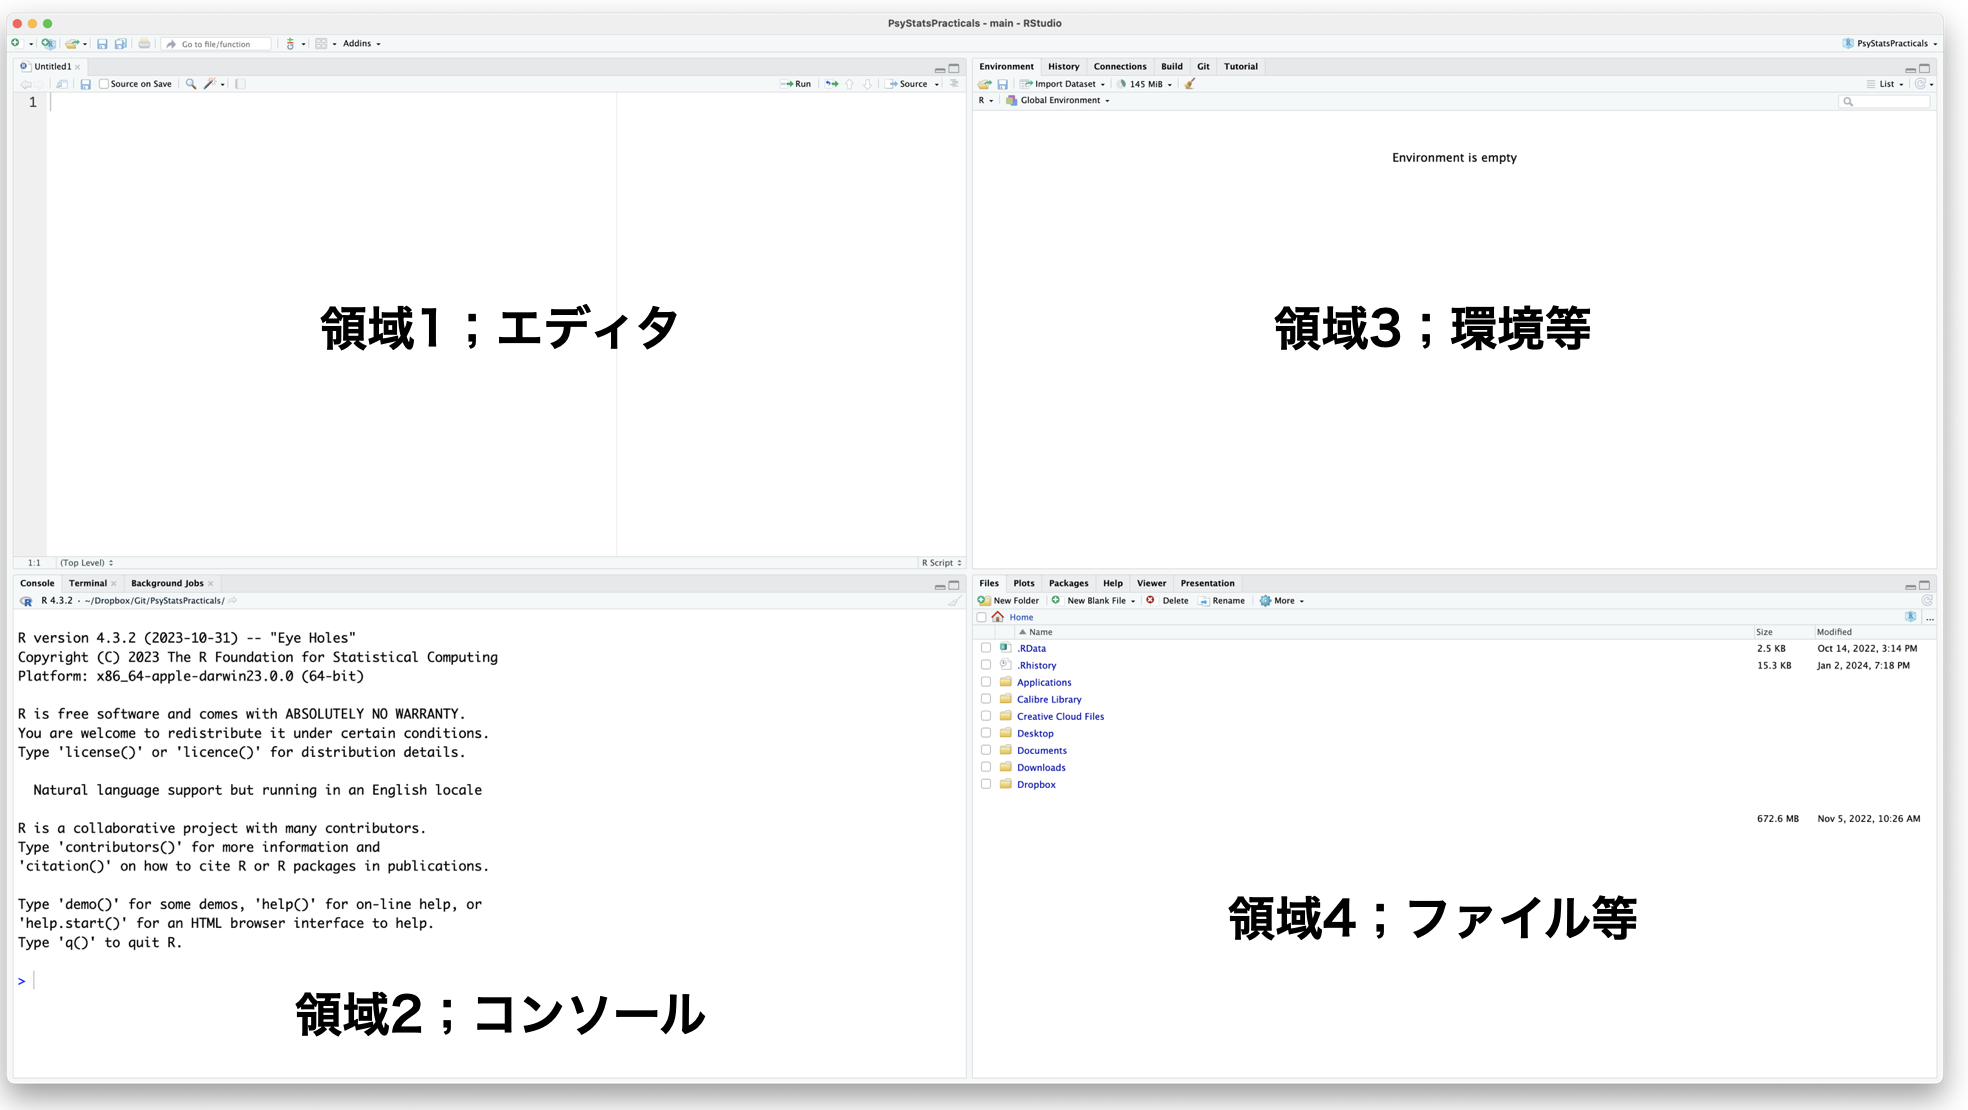
\includegraphics[keepaspectratio]{images/01_RStudioStart.png}}

}

\caption{RStudioの初期画面}

\end{figure}%

このペインのレイアウトは,メニューのTools \textgreater{} Global
Options\ldots{} \textgreater{} Pane
Layoutから変更することもできる。基本的に4分割であることに変わりはないが,自分が利用しやすい位置にレイアウトを変更するとよい。

\begin{figure}[H]

{\centering \pandocbounded{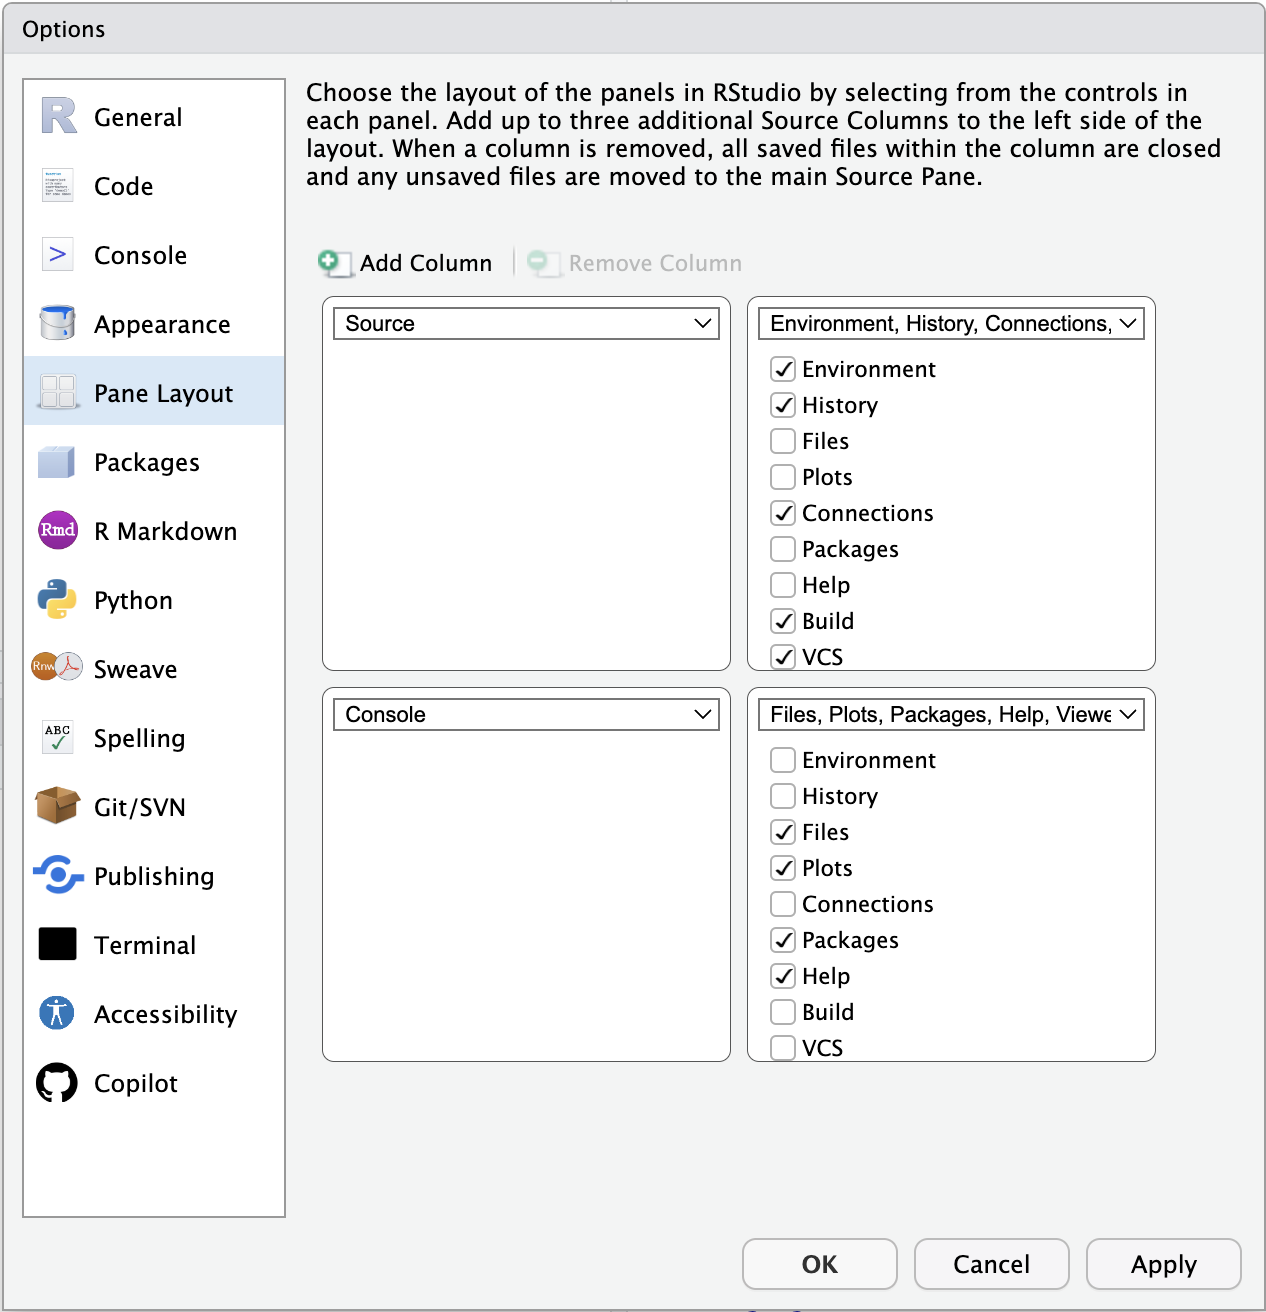
\includegraphics[keepaspectratio]{images/01_PaneLayout.png}}

}

\caption{レイアウト変更画面。このほかにも背景色などを変えることもできる}

\end{figure}%

以下,各ペイン(領域)が何をするところかを簡単に解説する。

\subsection{領域1;エディタ・ペイン}\label{ux9818ux57df1ux30a8ux30c7ux30a3ux30bfux30daux30a4ux30f3}

エディタ領域。Rのスクリプトはもちろん,レポートの文章など,基本的に入力するときはこのペインに書く。ここで作業するファイルの種類は,File
\textgreater{} New
Fileから見ると明らかなように,R言語だけでなくC言語,Python言語などのスクリプトや,Rmd,md,Qmd,HTMLなどのマークアップ言語,StanやSQLなど特殊な言語などにも対応している。ペインの右下に現在開かれているファイルの種類が表示されているのを確認しておこう。

R言語でスクリプトを書く例で解説しよう。Rは命令を逐次実行していくインタプリタ形式であり,ここに記述されたRコードを,右上のRunボタンでコンソールに送って計算を実行するように使う。一回の命令をコマンド,コマンドが積み重ねられた全体をスクリプト,あるいはプログラムと呼ぶ。複数のコマンドを実行したい場合は,エディタ領域で複数行選択してRunボタンを,スクリプトファイル全体を実行したいときはRunボタンのとなりにあるSourceを押す。CTRL+Enter(Macの場合はコマンド+Enter)でRunボタンのショートカットになる。

\subsection{領域2;コンソール・ペイン}\label{ux9818ux57df2ux30b3ux30f3ux30bdux30fcux30ebux30daux30a4ux30f3}

R単体で利用する場合は,ここのペインだけを利用するようなものである。すなわち,ここに示されているのがR本体というか,Rの計算機能そのものである。ここに「>」の記号が表示されているところをプロンプトといい,プロンプトが表示されているときはRが入力待ちの状態である。

Rは逐次的に計算を行うので,プロンプトのある状態でコマンドを入力すると計算結果が返される。
ここに直接コマンドを書いて行っても良いが,書き間違えたりすることもあるし,コマンドが複数行に渡ることが一般的になってくるので,エディタ領域に清書するつもりで記述していったほうがよい。ごくたまに,一時的に確認したいことがある時だけ,直接コンソールを触るようにすると良い。

なお,コンソールを綺麗にしたいときは右上の箒ボタンをおすとよい。

\subsection{領域3;環境ペイン}\label{ux9818ux57df3ux74b0ux5883ux30daux30a4ux30f3}

基本的にこのペインと次の領域4のペインは複数のタブが含まれる。Pane
Layoutでどちらにどのタブを含めるかを自分好みにカスタマイズすることもできる。ここでは代表的な2つのタブについてのみ言及する。

\textbf{Environment}タブは,Rの実行メモリ内に保管されている変数や関数などが表示されている。「変数や関数など」をまとめて\textbf{オブジェクト}というが,ここで内容や構造をGUIで確認することができる。

\textbf{History}タブは履歴である。これまでコンソールに送られてきたコマンドが順に記録されている。Historyタブからエディタ,コンソールにコマンドを送ることも可能であり,「さっきの命令をもう一度実行したい」といったときに参照すると良い。

\subsection{領域4;ファイルペイン}\label{ux9818ux57df4ux30d5ux30a1ux30a4ux30ebux30daux30a4ux30f3}

ここでも代表的なタブについてのみ解説する。

\textbf{Files}タブはMacでいうFinder,Windowsでいうエクスプローラーのような,ファイル操作画面である。フォルダの作成,ファイルの削除,リネーム,コピーなどの操作が可能である。

\textbf{Plot}タブはRコマンドで描画命令が出された時の結果がここに表示される。RStudioの利点の一つは,このPlotから図をファイルにExportすることが可能であり,その際にファイルサイズやファイル形式を指定できるところにある。

\textbf{Packages}タブは読み込まれているパッケージ,(読み込まれていないが)保管しているパッケージのリストが表示されている。新しくパッケージを導入するときも,ここのinstallボタンから可能であり,保管しているパッケージのアップデートもボタンひとつで可能である。なお,パッケージについては後ほど言及する。

\textbf{Help}タブはRコマンドでヘルプを表示する命令(\texttt{help}関数)が実行された時の結果が表示される領域である。ヘルプを使うことで関数の引数,戻り値,使用例などを参照できる。

\subsection{そのほかのタブ}\label{ux305dux306eux307bux304bux306eux30bfux30d6}

そのほか,表示の有無もオプションになっているようないくつかのタブについて,簡単に解説しておく。

\textbf{Connections}タブはRを外部データベースなどに繋げるときに参照する。大規模データをローカルにすべて取り込むことなく,SQLで必要なテーブルだけ取り出すといった操作をする際は必要になってくるだろう。

\textbf{Git}タブはR,とくにRプロジェクト(後述)のバージョンを管理するときに利用する。Gitとは複数のプログラマによって同時並行的にプログラムを作っていく時の管理システムである。時系列的な差分の記録を得意とするシステムなので,レポートの作成時などに応用すればラボノートの記録としても利用できる。

\textbf{Build}タブはRパッケージやWebサイトを構築するときに利用する。なおこの資料もRStudioを利用して作られており,資料を生成(原稿からHTMLやPDFにする)ときにはこのタブを利用している。

\textbf{Tutorial}タブはチュートリアルツアーを楽しむ時のタブである。

\textbf{Viewer}タブはRStudioで作られたHTMLやPDFなどを見るためのタブである。

\textbf{Presentation}タブはRStudioで作られたプレゼンテーションを見るためのタブである。

\textbf{Terminal}タブはWindows/MacでいうTerminal,Linuxでいう端末についてのタブであり,Rに限らず,コマンドラインを通じてOSに命令するときに使う。

\textbf{Background
Jobs}タブはその名の通りバックグラウンドで作業をさせるときに利用する。Rは基本的にシングルコアで計算が実行されるが,このタブを使ってスクリプトファイルをバックグラウンドで実行することで並列的に作業が可能になる。

\section{Rのパッケージ}\label{rux306eux30d1ux30c3ux30b1ux30fcux30b8}

Rは単体でも線形モデルなどの基本的な分析は可能であるが,より進んだ統計モデルを利用したい場合は専門の\textbf{パッケージ}を導入することになる。パッケージとは関数群のことであり,これもCRANやGithubなどインターネットを介して提供されている。ちなみに提供されているパッケージは,CRANで公開されているものだけで379,525件あり\footnote{2025年04月18日調べ},Github\footnote{Gitはバージョン管理システムであるが,これをインターネット上のサーバ(レポジトリ)で行うものをGithubという。RStudioはGithubとも連携しており,プロジェクトをGithubと紐づけることで簡単にバージョン管理ができる。しかもここで言及しているように,Github上でパッケージを公開することもできるので,最近はCRANの校閲を待たずに公開できるGithubが好まれている側面もある。}で公開されているものなど,CRANを介さないパッケージも少なくない。

パッケージを利用する際は,まずローカルにパッケージファイルをインストールしなければならない。その上で,Rを起動するごとに(セッションごとに),関数\texttt{library}でパッケージを呼び出して利用する。インストールを毎回行う必要はないことに注意。

インストールはRのコマンドでも可能だが,RStudioのPackagesペインを使って導入するのが簡単だろう。以下に,一部の有名かつ有用なパッケージ名とその簡単な説明を挙げる。本講義の中で使うものもあるので,事前に準備しておくことが望ましい。

\begin{itemize}
\tightlist
\item
  \emph{tidyverse}パッケージ\autocite{tidyverse};Rが飛躍的に使いやすくなったのは,このtidyverseパッケージ導入以後のことである。開発者のHadley
  WickhamはR業界で神と崇められており,R業界に与えたインパクトは大きい。このパッケージは「パッケージ群」「パッケージのパッケージ」であり,tidyverseとはtidyな(整然とした)verse(世界)というような意味合いである。このパッケージは統計分析モデルを提供するものではなく,その前のデータの\textbf{前処理}に関する便利な関数を提供する\footnote{実は統計データの解析にかかる時間のほとんどが,解析に適切な形にデータを整形する「前処理」に費やされる。前処理,別名データハンドリングをいかに上手く,素早く,直感的にできるかは,その後の分析にも影響するほど重要な手順であるため,tidyverseパッケージの登場はありがたかった。これを使ったデータハンドリングだけの専門書
    \textcite{Kinosady2021} が重宝されるほどである。}。このパッケージをインストールすると,関連する依存パッケージが次々取り込まれるので,少々時間がかかる。
\item
  \emph{psych}パッケージ\autocite{psych};名前の通り,心理学統計に関する統計モデルの多くが含まれている。特に特殊な相関係数や,因子分析モデルなどは非常に便利なので,インストールしておいて間違いない。
\item
  \emph{GPArotation}パッケージ\autocite{GPArotation};因子分析における因子軸の回転に使うパッケージ。
\item
  \emph{styler}パッケージ;スタイルを整えてくれるパッケージ。スクリプトの清書に便利。
\item
  \emph{lavaan}パッケージ\autocite{lavaan};潜在変数を含んだモデル(LAtent
  VAriable ANalysis)の分析,要するに構造方程式モデリング(Structural
  Equation Modeling;SEM,共分散構造分析ともいう)を実行するパッケージ。
\item
  \emph{ctv}パッケージ\autocite{CTV}; CRAN Task
  Viewsの略で,膨大に膨れ上がったCRANから必要なパッケージを見つけ出すのは困難であることから,ある程度のジャンルごとに関連しそうなパッケージをまとめて導入してくれるのがこのパッケージ。例えば,このパッケージをインストールした後で,\texttt{install.views("Psychometrics")}とすると,心理統計関係の多くのパッケージを次々導入してくれる。
\item
  \emph{cmdstanr}パッケージ\autocite{cmdstanr};複雑な統計モデルで利用される,確率的プログラミング言語stanをRから使うことができるようになるパッケージ。導入にはこのパッケージの他にもstanやコンパイル環境の準備が必要なので,\href{https://mc-stan.org/cmdstanr/articles/cmdstanr.html}{公式の導入サイト}も参考にしてほしい。
\end{itemize}

\section{RStudioのプロジェクト}\label{rstudioux306eux30d7ux30edux30b8ux30a7ux30afux30c8}

実際にRを使っていく前に,最後の準備としてRStudioにおけるプロジェクトについて解説しておく。

みなさんも,PCをつかって文書を作ったり保管したりするときに,フォルダにまとめて入れておくことがあるだろう。フォルダは例えば「文書」\textgreater「心理学」\textgreater「心理学統計演習」のように階層的に整理することが一般的で,そうしておくことで必要なファイルをすぐに取り出すことができる。

逆に言えば,こうしたフォルダ管理をしておかなければファイルがPCのなかで散乱してしまい,必要な情報を得るために逐一PCの中身を検索しなければならないだろう。

R/RStudioをつかった分析実践の場合も同様で,一回のテーマについて複数のファイル(スクリプトファイル,データファイル,画像ファイル,レポートなど文書ファイル等々)があり,シーンに合わせて(例えば「授業」「卒論」など)フォルダで管理することになる。

さらに,PC環境には作業フォルダ(Working
Directory)\footnote{ここでは,フォルダとディレクトリは同じ意味であると思ってもらって良い。一般に,CUIではディレクトリ,GUIではフォルダという用語が好まれる。語幹directにあるように,ファイルやアクセス先など具体的な指し示す先を強調しているのがディレクトリであり,それにファイル群などまとまった容れもの,という意味を付加したのがフォルダである。フォルダの方が言葉としてわかりやすいし。}という概念がある。たとえばR/RStudioを起動・実行しているときに,Rが「今どこで」実行されているか,どこを管理場所としているか,を表す概念である。例えばこの作業フォルダの中に\texttt{sample.csv}というファイルがあって,それをスクリプト上から読み込みたい,というコマンドを実行するのであれば,そのままファイル名を書けば良い。しかし別の場所にそのファイルが保存されているのなら,作業フォルダから見た相対的な位置を含めて指示してやるか(相対パス),あるいはPC環境全体からみた絶対的な位置を含めて(絶対パス)指示してやる必要がある。相対・絶対パスの違いは,「ここから二つ目の角を右」のように指示するか,住所で指示するかの違いであると考えれば良い。

ともあれ,この作業フォルダがどこに設定されているかは,実行するときに常に気にしていなければならない。ちなみにこの作業フォルダは,RStudioのファイルペイン・Filesタブでひらいているところとは\textbf{限らない}ことに注意してほしい。GUI上でエクスプローラ/Finderで開いたからといって,作業フォルダが自動的に切り替わるようにはなっていない。

そこでRStudioのプロジェクトである。RStudioには「プロジェクト」という概念があり,作業フォルダや環境の設定などをそこで管理することができる。新しくプロジェクトを始めるときはFile\textgreater New
Project,すでに一度プロジェクトを作っているときはFile \textgreater{}
Open
Projectとしてプロジェクトファイル(拡張子が.projのファイル)を開くようにする。そうすると,作業フォルダが当該フォルダに設定される。プロジェクトをGitに連携しておくとバージョン管理などもフォルダ単位で行える。

以後,本講義で外部ファイルを参照する場合,プロジェクトフォルダの中にそのファイルがあるものとして(パスを必要としない形で)論じるので注意されたし。

\section{課題}\label{ux8ab2ux984c}

\begin{itemize}
\tightlist
\item
  Rの最新版をCRANからダウンロードし,自分のPCにインストールしてください。
\item
  RStudioのDesktop版を\href{https://posit.co/download/rstudio-desktop/}{Posit社のサイト}からダウンロードし,自分のPCにインストールしてください。
\item
  RStidoを起動し,ペインレイアウトをデフォルトではない状態に並べ直してみてください。ソースペインを3列にするのも良いでしょう。
\item
  コンソールペインに書かれている文字を全て消去してみてください。
\item
  ファイルペインにあるFilesタブをつかって,色々なフォルダを開けてみたり,不要なファイルを削除したり,ファイル名を変更したりしてみてください。
\item
  ファイルペインにあるFilesタブを開き,\texttt{More}のところから\texttt{Go\ To\ Working\ Directory}を選択・実行してください。何か起こったでしょうか。
\item
  この授業のために,新しいプロジェクトを作成してください。プロジェクトは新しいフォルダでも,既存のフォルダでも構いません。
\item
  プロジェクトが開いた状態のとき,RStudioのウィンドウ・タブのどこかに「プロジェクト名」が表示されているはずです。確認してください。
\item
  またファイルペインのFilesタブから,色々なファイル操作をした上で,改めて\texttt{Go\ To\ Working\ Directory}をしてください。プロジェクトフォルダの中に戻ってこれたら成功です。
\item
  新しいRスクリプトファイルを開き,空白のままで結構ですからファイル名をつけて保存してください。
\item
  RStudioを終了あるいは最小化させ,OSのエクスプローラ/Finderから,プロジェクトフォルダに移動してください。先ほど作ったファイルが保存されていることを確認してください。
\item
  プロジェクトフォルダには,プロジェクト名+\texttt{.proj}というファイルが存在するはずです。これを開いて,RStudioのプロジェクトを開いてください。
\item
  RStudioのFile \textgreater{} Close
  Projectからプロジェクトを閉じてください。画面の細部でどこが変わったか,確認してください。
\item
  RStudioを終了し,再びRStudioを起動してください。起動の方法はプロジェクトファイルからでも,アプリケーションの起動でも構いません。起動後に,プロジェクトを開いてください(あるいはプロジェクトが開かれていることを確認してください。)。
\end{itemize}

\bookmarksetup{startatroot}

\chapter{Rの基礎}\label{sec-Rbase}

ここから実際にR/RStudioをつかった演習に入る。前回すでに言及したように,この講義用のプロジェクトを準備し,RStudioはプロジェクトが開かれた状態であることを前提に話を進める。

\section{Rで計算}\label{rux3067ux8a08ux7b97}

まずはRを使った計算である。Rスクリプトファイルを開き,最初の行に次の4行を入力してみよう。
各行を実行(Runボタン,あるいはctrl+enter)し,コンソールの結果を確認しよう。

\begin{Shaded}
\begin{Highlighting}[]
\DecValTok{1} \SpecialCharTok{+} \DecValTok{2}
\end{Highlighting}
\end{Shaded}

\begin{verbatim}
[1] 3
\end{verbatim}

\begin{Shaded}
\begin{Highlighting}[]
\DecValTok{2} \SpecialCharTok{{-}} \DecValTok{3}
\end{Highlighting}
\end{Shaded}

\begin{verbatim}
[1] -1
\end{verbatim}

\begin{Shaded}
\begin{Highlighting}[]
\DecValTok{3} \SpecialCharTok{*} \DecValTok{4}
\end{Highlighting}
\end{Shaded}

\begin{verbatim}
[1] 12
\end{verbatim}

\begin{Shaded}
\begin{Highlighting}[]
\DecValTok{6} \SpecialCharTok{/} \DecValTok{3}
\end{Highlighting}
\end{Shaded}

\begin{verbatim}
[1] 2
\end{verbatim}

それぞれ加減乗除の計算結果が正しく出ていることを確認してほしい。なお,出力のところに\texttt{{[}1{]}}とあるのは,Rがベクトルを演算の基本としているからで,回答ベクトルの第1要素を返していることを意味する。

四則演算の他に,次のような演算も可能である。

\begin{Shaded}
\begin{Highlighting}[]
\CommentTok{\# 整数の割り算}
\DecValTok{8} \SpecialCharTok{\%/\%} \DecValTok{3}
\end{Highlighting}
\end{Shaded}

\begin{verbatim}
[1] 2
\end{verbatim}

\begin{Shaded}
\begin{Highlighting}[]
\CommentTok{\# 余り}
\DecValTok{7} \SpecialCharTok{\%\%} \DecValTok{3}
\end{Highlighting}
\end{Shaded}

\begin{verbatim}
[1] 1
\end{verbatim}

\begin{Shaded}
\begin{Highlighting}[]
\CommentTok{\# 冪乗}
\DecValTok{2}\SpecialCharTok{\^{}}\DecValTok{3}
\end{Highlighting}
\end{Shaded}

\begin{verbatim}
[1] 8
\end{verbatim}

ここで,\texttt{\#}から始まる行は\textbf{コメントアウト}されたものとして,実際にコンソールに送られても計算されないことに注意しよう。スクリプトが単純なものである場合はコメントをつける必要はないが,複雑な計算になったり,他者と共有するときは「今どのような演算をしているか」を逐一解説するようにすると便利である。

実践上のテクニックとして,複数行を一括でコメントアウトしたり,アンコメント(コメントアウトを解除する)したりすることがある。スクリプトを複数行選択した上で,Codeメニューから\texttt{Comment/Uncomment\ Lines}を押すとコメント/アンコメントを切り替えられるので試してみよう。また,ショートカットキーも確認し,キーからコメント/アンコメントができるように慣れておくと良い(Ctrl+↑+C/Cmd+↑+C)。

One more
tip.コメントではなく,大きな段落的な区切り(セクション区切り)が欲しいこともあるかもしれない。Codeメニューの一番上に「Insert
Section」があるのでこれを選んでみよう。ショートカットキーから入力しても良い(Ctrl+↑+R/Cmd+↑+R)。セクション名を入力するボックスに適当な命名をすると,スクリプトにセクションが挿入される。次に示すのがセクションの例である。

\begin{Shaded}
\begin{Highlighting}[]
\CommentTok{\# 計算 {-}{-}{-}{-}{-}{-}{-}{-}{-}{-}{-}{-}{-}{-}{-}{-}{-}{-}{-}{-}{-}{-}{-}{-}{-}{-}{-}{-}{-}{-}{-}{-}{-}{-}{-}{-}{-}{-}{-}{-}{-}{-}{-}{-}{-}{-}{-}{-}{-}{-}{-}{-}{-}{-}{-}{-}{-}{-}{-}{-}{-}{-}}
\end{Highlighting}
\end{Shaded}

これはもちろん実行に影響を与えないが,ソースが長くなった場合はこのセクション単位で移動したり(スクリプトペインの左下),アウトラインを確認したり(スクリプトペインの右上にある横三本線)できるので,活用して欲しい。

\section{オブジェクト}\label{ux30aaux30d6ux30b8ux30a7ux30afux30c8}

Rでは変数,関数などあらゆるものを\textbf{オブジェクト}としてあつかう。オブジェクトには任意の名前をつけることができる(数字から始まる名前は不可)。
オブジェクトを作り,そこにある値を\textbf{代入}する例は次の通りである。

\begin{Shaded}
\begin{Highlighting}[]
\NormalTok{a }\OtherTok{\textless{}{-}} \DecValTok{1}
\NormalTok{b }\OtherTok{\textless{}{-}} \DecValTok{2}
\NormalTok{A }\OtherTok{\textless{}{-}} \DecValTok{3}
\NormalTok{a }\SpecialCharTok{+}\NormalTok{ b }\CommentTok{\# 1 + 2におなじ}
\end{Highlighting}
\end{Shaded}

\begin{verbatim}
[1] 3
\end{verbatim}

\begin{Shaded}
\begin{Highlighting}[]
\NormalTok{A }\SpecialCharTok{+}\NormalTok{ b }\CommentTok{\# 3 + 2におなじ}
\end{Highlighting}
\end{Shaded}

\begin{verbatim}
[1] 5
\end{verbatim}

ここでは数字をオブジェクトに保管し,オブジェクトを使って計算をしている。大文字と小文字が区別されてるため,計算結果が異なることに注意。

代入に使った記号\texttt{\textless{}-}は「小なり」と「ハイフン」であるが,左矢印のイメージである。次のように,\texttt{=}や\texttt{-\textgreater{}}を使うこともできる。

\begin{Shaded}
\begin{Highlighting}[]
\NormalTok{B }\OtherTok{\textless{}{-}} \DecValTok{5}
\DecValTok{7} \OtherTok{{-}\textgreater{}}\NormalTok{ A}
\end{Highlighting}
\end{Shaded}

ここで,二行目に\texttt{7\ -\textgreater{}\ A}を行った。先ほど\texttt{A\ \textless{}-\ 3}としたが,その後に\texttt{A}には7を代入し直したので,値は上書きされる。

\begin{Shaded}
\begin{Highlighting}[]
\NormalTok{A }\SpecialCharTok{+}\NormalTok{ b }\CommentTok{\# 7 + 2におなじ}
\end{Highlighting}
\end{Shaded}

\begin{verbatim}
[1] 9
\end{verbatim}

このように,オブジェクトに代入を重ねると,警告などなしに上書きされることに注意して欲しい。似たようなオブジェクト名を使い回していると,本来意図していたものと違う値・状態を保管していることになりかねないからである。

ちなみに,オブジェクトの中身を確認するためには,そのままオブジェクト名を入力すれば良い。より丁寧には,\texttt{print}関数を使う。

\begin{Shaded}
\begin{Highlighting}[]
\NormalTok{a}
\end{Highlighting}
\end{Shaded}

\begin{verbatim}
[1] 1
\end{verbatim}

\begin{Shaded}
\begin{Highlighting}[]
\FunctionTok{print}\NormalTok{(A)}
\end{Highlighting}
\end{Shaded}

\begin{verbatim}
[1] 7
\end{verbatim}

あるいは,RStudioのEnvironmentタブをみると,現在Rが保持しているオブジェクトが確認でき,単一の値の場合はValueセクションにオブジェクト名と値を見ることができる。

注意点として,オブジェクト名として,次の名前は使うことができない。>
break, else, for, if, in, next, function, repeat, return, while, TRUE,
FALSE.

これらはRで特別な意味を持つ\textbf{予約語}と呼ぶ。特に\texttt{TRUE}と\texttt{FALSE}は真・偽を表すもので,大文字の\texttt{T},\texttt{F}でも代用できるため,この一文字だけをオブジェクト名にするのは避けた方が良い。また,\texttt{T}と\texttt{F}は予約語ではないため,オブジェクト名として使用可能だが,混乱を避けるため使用は推奨されない。

\section{関数}\label{ux95a2ux6570}

関数は一般に\(y=f(x)\)と表されるが,要するに\(x\)を与えると\(y\)に形が変わる作用のことを指す。
プログラミング言語では一般に,\(x\)を\textbf{引数(ひきすう,argument)},\(y\)を\textbf{戻り値(もどりち,value)}という。以下,関数の使用例を挙げる。

\begin{Shaded}
\begin{Highlighting}[]
\FunctionTok{sqrt}\NormalTok{(}\DecValTok{16}\NormalTok{)}
\end{Highlighting}
\end{Shaded}

\begin{verbatim}
[1] 4
\end{verbatim}

\begin{Shaded}
\begin{Highlighting}[]
\FunctionTok{help}\NormalTok{(}\StringTok{"sqrt"}\NormalTok{)}
\end{Highlighting}
\end{Shaded}

最初の例は平方根square
rootを取る関数\texttt{sqrt}であり,引数として数字を与えるとその平方根が返される。第二の例は関数の説明を表示させる関数\texttt{help}であり,これを実行するとヘルプペインに関数の説明が表示される。

\section{変数の種類}\label{ux5909ux6570ux306eux7a2eux985e}

先ほどの\texttt{help}関数に与えた引数\texttt{"sqrt"}は文字列である。文字列であることを明示するためにダブルクォーテーション(\texttt{"})で囲っている(シングルクォーテーションで囲っても良い)。このように,Rが扱う変数は数字だけではない。変数の種類は数値型(numeric),文字型(character),論理値(logical)の3種類がある。

\begin{Shaded}
\begin{Highlighting}[]
\NormalTok{obj1 }\OtherTok{\textless{}{-}} \FloatTok{1.5}
\NormalTok{obj2 }\OtherTok{\textless{}{-}} \StringTok{"Hello"}
\NormalTok{obj3 }\OtherTok{\textless{}{-}} \ConstantTok{TRUE}
\end{Highlighting}
\end{Shaded}

数値型は整数(integer),実数(double)を含み\footnote{実数はreal
  numberじゃないのか,という指摘もあろうかとおもう。ここでは電子計算機上の数値の分類である,倍精度浮動小数点数(double-precision
  floating-point
  number)の意味である。倍精度とは単精度の倍を意味しており,単精度は32ビットを,倍精度は64ビットを単位として一つの数字を表す仕組みのことである。},そのほか,複素数型(complex),欠測値を表す\texttt{NA},非数値を表す\texttt{NaN}(Not
a Number),無限大を表す\texttt{Inf}などがある。

文字型はすでに説明した通りで,対になるクォーテーションが必要であることに注意してほしい。終わりを表すクォーテーションがなければ,Rは続く数字や文字も含めた「語」として処理する。この場合,enterキーを押しても文字入力が閉じられていないため,コンソールには「+」の表示が出る(この記号は前の行から入力が続いており,プロンプト状態ではないことを表している)。

また,文字型は当然のことながら四則演算の対象にならない。ただし,論理型の\texttt{TRUE/FALSE}はそれぞれ1,0に対応しているため,計算結果が表示される。次のコードを実行してこのことを確認しよう。

\begin{Shaded}
\begin{Highlighting}[]
\NormalTok{obj1 }\SpecialCharTok{+}\NormalTok{ obj2}
\NormalTok{obj1 }\SpecialCharTok{+}\NormalTok{ obj3}
\end{Highlighting}
\end{Shaded}

\section{オブジェクトの型}\label{ux30aaux30d6ux30b8ux30a7ux30afux30c8ux306eux578b}

ここまでみてきたように,数値や文字など(まとめて\textbf{リテラル}という)にも種類があるが,これをストックしておくものは全て\textbf{オブジェクト}である。オブジェクトとは変数のこと,と理解しても良いが,関数もオブジェクトに含まれる。

\subsection{ベクトル}\label{sec-vector}

Rのオブジェクトは単一の値しか持たないものではない。むしろ,複数の要素をセットで持つことができるのが特徴である。次に示すのは,\textbf{ベクトル}オブジェクトの例である。

\begin{Shaded}
\begin{Highlighting}[]
\NormalTok{vec1 }\OtherTok{\textless{}{-}} \FunctionTok{c}\NormalTok{(}\DecValTok{2}\NormalTok{, }\DecValTok{4}\NormalTok{, }\DecValTok{5}\NormalTok{)}
\NormalTok{vec2 }\OtherTok{\textless{}{-}} \DecValTok{1}\SpecialCharTok{:}\DecValTok{3}
\NormalTok{vec3 }\OtherTok{\textless{}{-}} \DecValTok{7}\SpecialCharTok{:}\DecValTok{5}
\NormalTok{vec4 }\OtherTok{\textless{}{-}} \FunctionTok{seq}\NormalTok{(}\AttributeTok{from =} \DecValTok{1}\NormalTok{, }\AttributeTok{to =} \DecValTok{7}\NormalTok{, }\AttributeTok{by =} \DecValTok{2}\NormalTok{)}
\NormalTok{vec5 }\OtherTok{\textless{}{-}} \FunctionTok{c}\NormalTok{(vec2, vec3)}
\end{Highlighting}
\end{Shaded}

それぞれのオブジェクトの中身を確認しよう。
最初の\texttt{c()}は結合combine関数である。また,コロン(\texttt{:})は連続する数値を与える。
\texttt{seq}関数は複数の引数を取るが,初期値,終了値,その間隔を指定した連続的なベクトルを生成する関数である。

ベクトルの計算は要素ごとに行われる。次のコードを実行し,どのように振る舞うか確認しよう。

\begin{Shaded}
\begin{Highlighting}[]
\NormalTok{vec1 }\SpecialCharTok{+}\NormalTok{ vec2}
\end{Highlighting}
\end{Shaded}

\begin{verbatim}
[1] 3 6 8
\end{verbatim}

\begin{Shaded}
\begin{Highlighting}[]
\NormalTok{vec3 }\SpecialCharTok{*} \DecValTok{2}
\end{Highlighting}
\end{Shaded}

\begin{verbatim}
[1] 14 12 10
\end{verbatim}

\begin{Shaded}
\begin{Highlighting}[]
\NormalTok{vec1 }\SpecialCharTok{+}\NormalTok{ vec5}
\end{Highlighting}
\end{Shaded}

\begin{verbatim}
[1]  3  6  8  9 10 10
\end{verbatim}

最後の計算でエラーが出なかったことに注目しよう。たとえば\texttt{vec1\ +\ vec4}はエラーになるが,ここでは計算結果が示されている(=エラーにはなっていない)。数学的には,長さの違うベクトルは計算が定義されていないのだが,\texttt{vec1}の長さは3,\texttt{vec5}の長さは6であった。\textbf{Rはベクトルを再利用する}ので,長いベクトルが短いベクトルの定数倍になるときは反復して利用される。すなわち,ここでは
\[ (2,4,5,2,4,5) + (1,2,3,7,6,5) = (3,6,8,9,10,10)\]

の計算がなされた。このRの仕様については,意図せぬ挙動にならぬよう注意しよう。

ベクトルの要素にアクセスするときは大括弧(\texttt{{[}\ {]}})を利用する。
特に第二・第三行目のコードの使い方を確認しておこう。大括弧の中は,要素番号でも良いし,真/偽の判断でも良いのである。この真偽判断による指定の方法は,条件節(\texttt{if}文)をつかって要素を指定できるため,有用である。

\begin{Shaded}
\begin{Highlighting}[]
\NormalTok{vec1[}\DecValTok{2}\NormalTok{]}
\end{Highlighting}
\end{Shaded}

\begin{verbatim}
[1] 4
\end{verbatim}

\begin{Shaded}
\begin{Highlighting}[]
\NormalTok{vec2[}\FunctionTok{c}\NormalTok{(}\DecValTok{1}\NormalTok{, }\DecValTok{3}\NormalTok{)]}
\end{Highlighting}
\end{Shaded}

\begin{verbatim}
[1] 1 3
\end{verbatim}

\begin{Shaded}
\begin{Highlighting}[]
\NormalTok{vec2[}\FunctionTok{c}\NormalTok{(}\ConstantTok{TRUE}\NormalTok{, }\ConstantTok{FALSE}\NormalTok{, }\ConstantTok{TRUE}\NormalTok{)]}
\end{Highlighting}
\end{Shaded}

\begin{verbatim}
[1] 1 3
\end{verbatim}

ここまで,ベクトルの要素は数値で説明してきたが,文字列などもベクトルとして利用できる。

\begin{Shaded}
\begin{Highlighting}[]
\NormalTok{words1 }\OtherTok{\textless{}{-}} \FunctionTok{c}\NormalTok{(}\StringTok{"Hello!"}\NormalTok{, }\StringTok{"Mr."}\NormalTok{, }\StringTok{"Monkey"}\NormalTok{, }\StringTok{"Magic"}\NormalTok{, }\StringTok{"Orchestra"}\NormalTok{)}
\NormalTok{words1[}\DecValTok{3}\NormalTok{]}
\end{Highlighting}
\end{Shaded}

\begin{verbatim}
[1] "Monkey"
\end{verbatim}

\begin{Shaded}
\begin{Highlighting}[]
\NormalTok{words2 }\OtherTok{\textless{}{-}}\NormalTok{ LETTERS[}\DecValTok{1}\SpecialCharTok{:}\DecValTok{10}\NormalTok{]}
\NormalTok{words2[}\DecValTok{8}\NormalTok{]}
\end{Highlighting}
\end{Shaded}

\begin{verbatim}
[1] "H"
\end{verbatim}

ここで\texttt{LETTERS}はアルファベット26文字が含まれている予約語ベクトルである。

ベクトルを引数に取る関数も多い。たとえば記述統計量である,平均,分散,標準偏差,合計などは,次のようにして計算する。

\begin{Shaded}
\begin{Highlighting}[]
\NormalTok{dat }\OtherTok{\textless{}{-}} \FunctionTok{c}\NormalTok{(}\DecValTok{12}\NormalTok{, }\DecValTok{18}\NormalTok{, }\DecValTok{23}\NormalTok{, }\DecValTok{35}\NormalTok{, }\DecValTok{22}\NormalTok{)}
\FunctionTok{mean}\NormalTok{(dat) }\CommentTok{\# 平均}
\end{Highlighting}
\end{Shaded}

\begin{verbatim}
[1] 22
\end{verbatim}

\begin{Shaded}
\begin{Highlighting}[]
\FunctionTok{var}\NormalTok{(dat) }\CommentTok{\# 分散}
\end{Highlighting}
\end{Shaded}

\begin{verbatim}
[1] 71.5
\end{verbatim}

\begin{Shaded}
\begin{Highlighting}[]
\FunctionTok{sd}\NormalTok{(dat) }\CommentTok{\# 標準偏差}
\end{Highlighting}
\end{Shaded}

\begin{verbatim}
[1] 8.455767
\end{verbatim}

\begin{Shaded}
\begin{Highlighting}[]
\FunctionTok{sum}\NormalTok{(dat) }\CommentTok{\# 合計}
\end{Highlighting}
\end{Shaded}

\begin{verbatim}
[1] 110
\end{verbatim}

他にも最大値\texttt{max}や最小値\texttt{min},中央値\texttt{median}などの関数が利用可能である。

\subsection{行列}\label{ux884cux5217}

数学では線形代数でベクトルを扱うが,同時にベクトルが複数並んだ二次元の行列も扱うだろう。
Rでも行列のように配置したオブジェクトを利用できる。

次のコードで作られる行列\(A\),\(B\)がどのようなものか確認しよう。

\begin{Shaded}
\begin{Highlighting}[]
\NormalTok{A }\OtherTok{\textless{}{-}} \FunctionTok{matrix}\NormalTok{(}\DecValTok{1}\SpecialCharTok{:}\DecValTok{6}\NormalTok{, }\AttributeTok{ncol =} \DecValTok{2}\NormalTok{)}
\NormalTok{B }\OtherTok{\textless{}{-}} \FunctionTok{matrix}\NormalTok{(}\DecValTok{1}\SpecialCharTok{:}\DecValTok{6}\NormalTok{, }\AttributeTok{ncol =} \DecValTok{2}\NormalTok{, }\AttributeTok{byrow =}\NormalTok{ T)}
\end{Highlighting}
\end{Shaded}

行列を作る関数\texttt{matrix}は,引数として要素,列数(\texttt{ncol}),行数(\texttt{nrow}),要素配列を行ごとにするかどうかの指定(\texttt{byrow})をとる。ここでは要素を\texttt{1:6}としており,1から6までの連続する整数をあたえている。\texttt{ncol}で2列であることを明示しているので,\texttt{nrow}で行数を指定してやる必要はない。\texttt{byrow}の有無でどのように数字が変わっているかは表示させれば一目瞭然であろう。

与える要素が行数\(\times\)列数に一致しておらず,ベクトルの再利用も不可能な場合はエラーが返ってくる。

また,ベクトルの要素指定のように,行列も大括弧を使って要素を指定することができる。行,列の順に指定し,行だけ,列だけの指定も可能である。

\begin{Shaded}
\begin{Highlighting}[]
\NormalTok{A[}\DecValTok{2}\NormalTok{, }\DecValTok{2}\NormalTok{]}
\end{Highlighting}
\end{Shaded}

\begin{verbatim}
[1] 5
\end{verbatim}

\begin{Shaded}
\begin{Highlighting}[]
\NormalTok{A[}\DecValTok{1}\NormalTok{, ]}
\end{Highlighting}
\end{Shaded}

\begin{verbatim}
[1] 1 4
\end{verbatim}

\begin{Shaded}
\begin{Highlighting}[]
\NormalTok{A[, }\DecValTok{2}\NormalTok{]}
\end{Highlighting}
\end{Shaded}

\begin{verbatim}
[1] 4 5 6
\end{verbatim}

\subsection{リスト型}\label{ux30eaux30b9ux30c8ux578b}

行列はサイズの等しいベクトルのセットであるが,サイズの異なる要素をまとめて一つのオブジェクトとして保管しておきたいときはリスト型をつかう。

\begin{Shaded}
\begin{Highlighting}[]
\NormalTok{Obj1 }\OtherTok{\textless{}{-}} \FunctionTok{list}\NormalTok{(}\DecValTok{1}\SpecialCharTok{:}\DecValTok{4}\NormalTok{, }\FunctionTok{matrix}\NormalTok{(}\DecValTok{1}\SpecialCharTok{:}\DecValTok{6}\NormalTok{, }\AttributeTok{ncol =} \DecValTok{2}\NormalTok{), }\DecValTok{3}\NormalTok{)}
\end{Highlighting}
\end{Shaded}

このオブジェクトの第一要素(\texttt{{[}{[}1{]}{]}})はベクトル,第二要素は行列,第三要素は要素1つのベクトル(スカラー)である。オブジェクトの要素の要素(ex.第二要素の行列の2行3列目の要素)にどのようにアクセスすれば良いか,考えてみよう。

このリストは要素へのアクセスの際に\texttt{{[}{[}1{]}{]}}など数字が必要だが,要素に名前をつけることで利便性が増す。

\begin{Shaded}
\begin{Highlighting}[]
\NormalTok{Obj2 }\OtherTok{\textless{}{-}} \FunctionTok{list}\NormalTok{(}
  \AttributeTok{vec1 =} \DecValTok{1}\SpecialCharTok{:}\DecValTok{5}\NormalTok{,}
  \AttributeTok{mat1 =} \FunctionTok{matrix}\NormalTok{(}\DecValTok{1}\SpecialCharTok{:}\DecValTok{10}\NormalTok{, }\AttributeTok{nrow =} \DecValTok{5}\NormalTok{),}
  \AttributeTok{char1 =} \StringTok{"YMO"}
\NormalTok{)}
\end{Highlighting}
\end{Shaded}

この名前付きリストの要素にアクセスするときは,\texttt{\$}記号を用いることができる。

\begin{Shaded}
\begin{Highlighting}[]
\NormalTok{Obj2}\SpecialCharTok{$}\NormalTok{vec1}
\end{Highlighting}
\end{Shaded}

\begin{verbatim}
[1] 1 2 3 4 5
\end{verbatim}

これを踏まえて,名前付きリストの要素の要素にアクセスするにはどうすれば良いか,考えてみよう。

リスト型はこのように,要素のサイズ・長さを問わないため,いろいろなものを保管しておくことができる。統計関数の結果はリスト型で得られることが多く,そのような場合,リストの要素も長くなりがちである。リストがどのような構造を持っているかを見るために,\texttt{str}関数が利用できる。

\begin{Shaded}
\begin{Highlighting}[]
\FunctionTok{str}\NormalTok{(Obj2)}
\end{Highlighting}
\end{Shaded}

\begin{verbatim}
List of 3
 $ vec1 : int [1:5] 1 2 3 4 5
 $ mat1 : int [1:5, 1:2] 1 2 3 4 5 6 7 8 9 10
 $ char1: chr "YMO"
\end{verbatim}

\texttt{str}関数の返す結果と同じものが,RStudioのEnvironmentタブからオブジェクトを見ることでも得られる。
また,リストの要素としてリストを持つ,すなわち階層的になることもある。そのような場合,必要としている要素にどのようにアクセスすれば良いか,確認しておこう。

\begin{Shaded}
\begin{Highlighting}[]
\NormalTok{Obj3 }\OtherTok{\textless{}{-}} \FunctionTok{list}\NormalTok{(Obj1, }\AttributeTok{Second =}\NormalTok{ Obj2)}
\FunctionTok{str}\NormalTok{(Obj3)}
\end{Highlighting}
\end{Shaded}

\begin{verbatim}
List of 2
 $       :List of 3
  ..$ : int [1:4] 1 2 3 4
  ..$ : int [1:3, 1:2] 1 2 3 4 5 6
  ..$ : num 3
 $ Second:List of 3
  ..$ vec1 : int [1:5] 1 2 3 4 5
  ..$ mat1 : int [1:5, 1:2] 1 2 3 4 5 6 7 8 9 10
  ..$ char1: chr "YMO"
\end{verbatim}

\subsection{データフレーム型}\label{ux30c7ux30fcux30bfux30d5ux30ecux30fcux30e0ux578b}

リスト型は要素のサイズを問わないことはすでに述べた。しかしデータ解析を行うときは得てして,2次元スプレッドシートのような形式である。すなわち一行に1オブザベーション,各列は変数を表すといった具合である。このように矩形かつ,列に変数名を持たせることができる特殊なリスト型を\textbf{データフレーム型}という。以下はそのようなオブジェクトの例である。

\begin{Shaded}
\begin{Highlighting}[]
\NormalTok{df }\OtherTok{\textless{}{-}} \FunctionTok{data.frame}\NormalTok{(}
  \AttributeTok{name =} \FunctionTok{c}\NormalTok{(}\StringTok{"Ishino"}\NormalTok{, }\StringTok{"Pierre"}\NormalTok{, }\StringTok{"Marin"}\NormalTok{),}
  \AttributeTok{origin =} \FunctionTok{c}\NormalTok{(}\StringTok{"Shizuoka"}\NormalTok{, }\StringTok{"Shizuoka"}\NormalTok{, }\StringTok{"Hokkaido"}\NormalTok{),}
  \AttributeTok{height =} \FunctionTok{c}\NormalTok{(}\DecValTok{170}\NormalTok{, }\DecValTok{180}\NormalTok{, }\DecValTok{160}\NormalTok{),}
  \AttributeTok{salary =} \FunctionTok{c}\NormalTok{(}\DecValTok{1000}\NormalTok{, }\DecValTok{20}\NormalTok{, }\DecValTok{800}\NormalTok{)}
\NormalTok{)}
\CommentTok{\# 内容を表示させる}
\NormalTok{df}
\end{Highlighting}
\end{Shaded}

\begin{verbatim}
    name   origin height salary
1 Ishino Shizuoka    170   1000
2 Pierre Shizuoka    180     20
3  Marin Hokkaido    160    800
\end{verbatim}

\begin{Shaded}
\begin{Highlighting}[]
\CommentTok{\# 構造を確認する}
\FunctionTok{str}\NormalTok{(df)}
\end{Highlighting}
\end{Shaded}

\begin{verbatim}
'data.frame':   3 obs. of  4 variables:
 $ name  : chr  "Ishino" "Pierre" "Marin"
 $ origin: chr  "Shizuoka" "Shizuoka" "Hokkaido"
 $ height: num  170 180 160
 $ salary: num  1000 20 800
\end{verbatim}

ところで,心理統計の初歩としてStevensの尺度水準\autocite{stevens1946}について学んだことと思う。そこでは数値が,その値に許される演算のレベルをもとに,名義,順序,間隔,比率尺度水準という4つの段階に分類される。間隔・比率尺度水準の数値は数学的な計算を施しても良いが,順序尺度水準や名義尺度水準の数字はそのような計算が許されない(ex.2番目に好きな人と3番目に好きな人が一緒になっても,1番好きな人に敵わない。)

Rには,こうした尺度水準に対応した数値型がある。間隔・比率尺度水準は計算可能なので\texttt{numeric}型でよいが,名義尺度水準は\texttt{factor}型(要因型,因子型とも呼ばれる),順序尺度水準は\texttt{ordered.factor}型と呼ばれるものである。

factor型の変数の例を挙げる。すでに文字型として入っているものをfactor型として扱うよう変換するためには,\texttt{as.factor}関数が利用できる。

\begin{Shaded}
\begin{Highlighting}[]
\NormalTok{df}\SpecialCharTok{$}\NormalTok{origin }\OtherTok{\textless{}{-}} \FunctionTok{as.factor}\NormalTok{(df}\SpecialCharTok{$}\NormalTok{origin)}
\NormalTok{df}\SpecialCharTok{$}\NormalTok{origin}
\end{Highlighting}
\end{Shaded}

\begin{verbatim}
[1] Shizuoka Shizuoka Hokkaido
Levels: Hokkaido Shizuoka
\end{verbatim}

要素を表示させて見ると明らかなように,値としては\texttt{Shizuoka},\texttt{Shizuoka},\texttt{Hokkaido}の3つあるが,レベル(水準)は\texttt{Shizuoka},\texttt{Hokkaido}の2つである。このようにfactor型にしておくと,カテゴリとして使えて便利である。

次に示すのは順序つきfactor型変数の例である。

\begin{Shaded}
\begin{Highlighting}[]
\CommentTok{\# 順序付き要因型の例}
\NormalTok{ratings }\OtherTok{\textless{}{-}} \FunctionTok{factor}\NormalTok{(}\FunctionTok{c}\NormalTok{(}\StringTok{"低い"}\NormalTok{, }\StringTok{"高い"}\NormalTok{, }\StringTok{"中程度"}\NormalTok{, }\StringTok{"高い"}\NormalTok{, }\StringTok{"低い"}\NormalTok{),}
  \AttributeTok{levels =} \FunctionTok{c}\NormalTok{(}\StringTok{"低い"}\NormalTok{, }\StringTok{"中程度"}\NormalTok{, }\StringTok{"高い"}\NormalTok{),}
  \AttributeTok{ordered =} \ConstantTok{TRUE}
\NormalTok{)}
\CommentTok{\# ratingsの内容と型を確認}
\FunctionTok{print}\NormalTok{(ratings)}
\end{Highlighting}
\end{Shaded}

\begin{verbatim}
[1] 低い   高い   中程度 高い   低い  
Levels: 低い < 中程度 < 高い
\end{verbatim}

集計の際などはfactor型と違わないため,使用例は少ないかもしれない。しかしRは統計モデルを適用する時に,尺度水準に対応した振る舞いをするものがあるので,データの尺度水準を丁寧に設定しておくのも良いだろう。

データフレームの要素へのアクセスは,基本的に変数名を介してのものになるだろう。たとえば先ほどのオブジェクト\texttt{df}
の数値変数に統計処理をしたい場合は,次のようにすると良い。

\begin{Shaded}
\begin{Highlighting}[]
\FunctionTok{mean}\NormalTok{(df}\SpecialCharTok{$}\NormalTok{height)}
\end{Highlighting}
\end{Shaded}

\begin{verbatim}
[1] 170
\end{verbatim}

\begin{Shaded}
\begin{Highlighting}[]
\FunctionTok{sum}\NormalTok{(df}\SpecialCharTok{$}\NormalTok{salary)}
\end{Highlighting}
\end{Shaded}

\begin{verbatim}
[1] 1820
\end{verbatim}

また,データフレームオブジェクトを一括で要約する関数もある。

\begin{Shaded}
\begin{Highlighting}[]
\FunctionTok{summary}\NormalTok{(df)}
\end{Highlighting}
\end{Shaded}

\begin{verbatim}
     name                origin      height        salary      
 Length:3           Hokkaido:1   Min.   :160   Min.   :  20.0  
 Class :character   Shizuoka:2   1st Qu.:165   1st Qu.: 410.0  
 Mode  :character                Median :170   Median : 800.0  
                                 Mean   :170   Mean   : 606.7  
                                 3rd Qu.:175   3rd Qu.: 900.0  
                                 Max.   :180   Max.   :1000.0  
\end{verbatim}

\section{外部ファイルの読み込み}\label{ux5916ux90e8ux30d5ux30a1ux30a4ux30ebux306eux8aadux307fux8fbcux307f}

解析の実際では,データセットを手入力することはなく,データベースから取り出してくるか,別ファイルから読み込むことが一般的であろう。

統計パッケージの多くは独自のファイル形式を持っており,Rにはそれぞれに対応した読み込み関数も用意されているが,ここでは最もプレーンな形でのデータであるCSV形式からの読み込み例を示す。

サンプルデータ\url{Baseball.csv}を読み込むことを考える。なおこのデータはUTF-8形式で保存されている\footnote{UTF-8というのは文字コードの一種で,0と1からなる機械のデータを人間語に翻訳するためのコードであり,世界的にもっとも一般的な文字コードである。しかしWindowsOSはいまだにデフォルトでShift-JISというローカルな文字コードにしているため,このファイルを一度Windows機のExcelなどで開くと文字化けし,以下の手続が正常に作用しなくなることがよくある。本講義で使う場合は,ダウンロード後にExcelなどで開くことなく,直接Rから読み込むようにされたし。}。これを読み込むには,Rがデフォルトで持っている関数\texttt{read.csv}が使える。

\begin{Shaded}
\begin{Highlighting}[]
\NormalTok{dat }\OtherTok{\textless{}{-}} \FunctionTok{read.csv}\NormalTok{(}\StringTok{"Baseball.csv"}\NormalTok{)}
\FunctionTok{head}\NormalTok{(dat)}
\end{Highlighting}
\end{Shaded}

\begin{verbatim}
      Year       Name team salary bloodType height weight UniformNum position
1 2011年度 永川 勝浩 Carp  12000       O型    188     97         20     投手
2 2011年度 前田 健太 Carp  12000       A型    182     73         18     投手
3 2011年度 栗原 健太 Carp  12000       O型    183     95          5   内野手
4 2011年度 東出 輝裕 Carp  10000       A型    171     73          2   内野手
5 2011年度   シュルツ Carp   9000      不明    201    100         70     投手
6 2011年度   大竹 寛 Carp   8000       B型    183     90         17     投手
  Games AtBats Hit HR Win Lose Save Hold
1    19     NA  NA NA   1    2    0    0
2    31     NA  NA NA  10   12    0    0
3   144    536 157 17  NA   NA   NA   NA
4   137    543 151  0  NA   NA   NA   NA
5    19     NA  NA NA   0    0    0    9
6     6     NA  NA NA   1    1    0    0
\end{verbatim}

\begin{Shaded}
\begin{Highlighting}[]
\FunctionTok{str}\NormalTok{(dat)}
\end{Highlighting}
\end{Shaded}

\begin{verbatim}
'data.frame':   7944 obs. of  17 variables:
 $ Year      : chr  "2011年度" "2011年度" "2011年度" "2011年度" ...
 $ Name      : chr  "永川 勝浩" "前田 健太" "栗原 健太" "東出 輝裕" ...
 $ team      : chr  "Carp" "Carp" "Carp" "Carp" ...
 $ salary    : int  12000 12000 12000 10000 9000 8000 8000 7500 7000 6600 ...
 $ bloodType : chr  "O型" "A型" "O型" "A型" ...
 $ height    : int  188 182 183 171 201 183 177 173 176 188 ...
 $ weight    : int  97 73 95 73 100 90 82 73 80 97 ...
 $ UniformNum: int  20 18 5 2 70 17 31 6 1 43 ...
 $ position  : chr  "投手" "投手" "内野手" "内野手" ...
 $ Games     : int  19 31 144 137 19 6 110 52 52 40 ...
 $ AtBats    : int  NA NA 536 543 NA NA 299 192 44 149 ...
 $ Hit       : int  NA NA 157 151 NA NA 60 41 11 35 ...
 $ HR        : int  NA NA 17 0 NA NA 4 2 0 1 ...
 $ Win       : int  1 10 NA NA 0 1 NA NA NA NA ...
 $ Lose      : int  2 12 NA NA 0 1 NA NA NA NA ...
 $ Save      : int  0 0 NA NA 0 0 NA NA NA NA ...
 $ Hold      : int  0 0 NA NA 9 0 NA NA NA NA ...
\end{verbatim}

ここで\texttt{head}関数はデータフレームなどオブジェクトの冒頭部分(デフォルトでは6行分)を表示させるものである。また,\texttt{str}関数の結果から明らかなように,読み込んだファイルが自動的にデータフレーム型になっている。

ちなみに,サンプルデータにおいて欠測値に該当する箇所には\texttt{NA}の文字が入っていた。\texttt{read.csv}関数では,欠測値はデフォルトで文字列''NA''としている。しかし,実際は別の文字(ex.ピリオド)や,特定の値(ex.9999)の場合もあるだろう。その際は,オプション\texttt{na.strings}で「欠測値として扱う値」を指示すれば良い。

\section{おまけ;スクリプトの清書}\label{ux304aux307eux3051ux30b9ux30afux30eaux30d7ux30c8ux306eux6e05ux66f8}

さて,ここまでスクリプトを書いてきたことで,そこそこ長いスクリプトファイルができたことと思う。
スクリプトの記述については,もちろん「動けばいい」という考え方もあるが,美しくかけていたほうがなお良いだろう。「美しい」をどのように定義するかは異論あるだろうが,一般に「コード規約」と呼ばれる清書方法がある。ここでは細部まで言及しないが,RStudioのCodeメニューからReformat
Codeを実行してみよう。スクリプトファイルが綺麗に整ったように見えないだろうか?

美しいコードはデバッグにも役立つ。時折Reformatすることを心がけよう。

\section{課題}\label{ux8ab2ux984c-1}

\begin{itemize}
\item
  Rを起動し,新しいスクリプトファイルを作成してください。そのファイル内で,2つの整数を宣言し,足し算を行い,結果をコンソールに表示してください。
\item
  スクリプトに次の計算を書き,実行してください。

  \begin{itemize}
  \tightlist
  \item
    \(\frac{5}{6} + \frac{1}{3}\)
  \item
    \(9.6 \div 4\)
  \item
    \(2.3 + \frac{1}{2}\)
  \item
    \(3\times (2.2 + \frac{4}{5})\)
  \item
    \((-2)^4\)
  \item
    \(2\sqrt{2} \times \sqrt{3}\)
  \item
    \(2\log_e 25\)
  \end{itemize}
\item
  Rのスクリプトファイル内で,ベクトルを作成してください。ベクトルには1から10までの整数を格納してください。その後,ベクトルの要素の合計と平均を計算してください。ベクトルを合計する関数は\texttt{sum},平均は\texttt{mean}です。
\item
  次の表をリスト型オブジェクト\texttt{Tbl}にしてください。
\end{itemize}

\begin{longtable}[]{@{}lrrr@{}}
\toprule\noalign{}
Name & Pop & Area & Density \\
\midrule\noalign{}
\endhead
\bottomrule\noalign{}
\endlastfoot
Tokyo & 1,403 & 2,194 & 6,397 \\
Beijing & 2,170 & 16,410 & 1,323 \\
Seoul & 949 & 605 & 15,688 \\
\end{longtable}

\begin{itemize}
\item
  先ほど作った\texttt{Tbl}オブジェクトの,東京(Tokyo)の面積(Area)の値を表示させてください(リスト要素へのアクセス)
\item
  \texttt{Tbl}オブジェクトの人口(Pop)変数の平均を計算してください。
\item
  \texttt{Tbl}オブジェクトをデータフレーム型オブジェクト\texttt{df2}に変換してください。新たに作り直しても良いですし,\texttt{as.data.frame}関数を使っても良い。
\item
  Rのスクリプトを使用して,別のサンプルデータ\url{Baseball2022.csv}
  ファイルを読み込み,データフレーム\texttt{dat}に格納してください。ただし,このファイルの欠測値は\(999\)という数値になっています。
\item
  読み込んだ\texttt{dat}の冒頭の10行を表示してみてください。
\item
  読み込んだ\texttt{dat}に\texttt{summary}関数を適用してください。
\item
  このデータセットの変数\texttt{team}は名義尺度水準です。Factor型にしてください。他にもFactor型にすべき変数が2つありますので,それらも同様に型を変換してください。
\item
  このデータセットの変数の中で,数値データに対して平均,分散,標準偏差,最大値,最小値,中央値を
  それぞれ算出してください。
\item
  課題を記述したスクリプトファイルに対して,Reformatなどで整形してください。
\end{itemize}

\bookmarksetup{startatroot}

\chapter{Rによるデータハンドリング}\label{rux306bux3088ux308bux30c7ux30fcux30bfux30cfux30f3ux30c9ux30eaux30f3ux30b0}

心理学を始め,データを扱うサイエンスでは,データ収集の計画,実行と,データに基づいた解析結果,それを踏まえてのコミュニケーションとの間に,「データをわかりやすい形に加工し,可視化し,分析する」という手順がある。このデータの加工を\textbf{データハンドリング}という。統計といえば「分析」に注目されがちだが,実際にはデータハンドリングと可視化のステップが最も時間を必要とし,重要なプロセスである。

\section{tidyverseの導入}\label{tidyverseux306eux5c0eux5165}

本講義では\texttt{tidyverse}をつかったデータハンドリングを扱う。\texttt{tidyverse}は,データに対する統一的な設計方針を表す概念でもあり,具体的にはそれを実装したパッケージ名でもある。まずは\texttt{tidyverse}パッケージをインストール(ダウンロード)し,次のコードでRに読み込んでおく。

\begin{Shaded}
\begin{Highlighting}[]
\NormalTok{pacman}\SpecialCharTok{::}\FunctionTok{p\_load}\NormalTok{(tidyverse)}
\end{Highlighting}
\end{Shaded}

Attaching core tidyverse
packages,と表示され,複数のパッケージ名にチェックマークが入っていたものが表示されただろう。\texttt{tidyverse}パッケージはこれらの下位パッケージを含むパッケージ群である。これに含まれる\texttt{dplyr},\texttt{tidyr}パッケージはデータの整形に,\texttt{readr}はファイルの読み込みに,\texttt{forcats}はFactor型変数の操作に,\texttt{stringr}は文字型変数の操作に,\texttt{lubridate}は日付型変数の操作に,\texttt{tibble}はデータフレーム型オブジェクトの操作に,\texttt{purrr}はデータに適用する関数に,\texttt{ggplot2}は可視化に特化したパッケージである。

続いてConflictsについての言及がある。\texttt{tidyverse}パッケージに限らず,パッケージを読み込むと表示されることのあるこの警告は,「関数名の衝突」を意味している。ここまで,Rを起動するだけで,\texttt{sqrt},\texttt{mean}などの関数が利用できた。これはRの基本関数であるが,具体的には\texttt{base}パッケージに含まれた関数である。Rは起動時に\texttt{base}などいくつかのパッケージを自動的に読み込んでいるのである。これに別途パッケージを読み込むとき,あとで読み込まれたパッケージが同名の関数を使っていることがある。このとき,関数名は後から読み込んだもので上書きされる。そのことについての警告が表示されているのである。具体的にみると,\texttt{dplyr::filter()\ masks\ stats::filter()}とあるのは,最初に読み込んでいた\texttt{stats}パッケージの\texttt{filter}関数は,(\texttt{tidyverse}パッケージに含まれる)\texttt{dplyr}パッケージのもつ同名の関数で上書きされ,今後はこちらが優先的に利用されるよ,ということを示している。

このような同音異字関数は,関数を特定するときに混乱を招くかもしれない。あるパッケージの関数であることを明示したい場合は,この警告文にあるように,パッケージ名\texttt{::}関数名,という書き方にすると良い。

\section{パイプ演算子}\label{ux30d1ux30a4ux30d7ux6f14ux7b97ux5b50}

続いてパイプ演算子について解説する。パイプ演算子は\texttt{tidyverse}パッケージに含まれていた\texttt{magrittr}パッケージで導入されたもので,これによってデータハンドリングの利便性が一気に向上した。そこでRもver
4.2からこの演算子を導入し,特段パッケージのインストールを必要としなくとも使えるようになった。このR本体のパイプ演算子のことを,\texttt{tidyverse}のそれと区別して,ネイティブパイプと呼ぶこともある。

ともあれこのパイプ演算子がいかに優れたものであるかを解説しよう。次のスクリプトは,あるデータセットの標準偏差を計算するものである\footnote{もちろん\texttt{sd(dat)}
  の一行で済む話だが,ここでは説明のために各ステップを書き下している。もっとも,\texttt{sd}関数で計算されるのは\(n-1\)で割った不偏分散の平方根であり,標本標準偏差とは異なるものである。}。数式で表現すると次の通り。ここで\(\bar{x}\)はデータベクトル\(x\)の算術平均。
\[v = \sqrt{\frac{1}{n}\sum_{i=1}^n (x_i - \bar{x})^2}\]

\begin{Shaded}
\begin{Highlighting}[]
\NormalTok{dat }\OtherTok{\textless{}{-}} \FunctionTok{c}\NormalTok{(}\DecValTok{10}\NormalTok{, }\DecValTok{13}\NormalTok{, }\DecValTok{15}\NormalTok{, }\DecValTok{12}\NormalTok{, }\DecValTok{14}\NormalTok{) }\CommentTok{\# データ}
\NormalTok{M }\OtherTok{\textless{}{-}} \FunctionTok{mean}\NormalTok{(dat) }\CommentTok{\# 平均}
\NormalTok{dev }\OtherTok{\textless{}{-}}\NormalTok{ dat }\SpecialCharTok{{-}}\NormalTok{ M }\CommentTok{\# 平均偏差}
\NormalTok{pow }\OtherTok{\textless{}{-}}\NormalTok{ dev}\SpecialCharTok{\^{}}\DecValTok{2} \CommentTok{\# 平均偏差の2乗}
\NormalTok{variance }\OtherTok{\textless{}{-}} \FunctionTok{mean}\NormalTok{(pow) }\CommentTok{\# 平均偏差の2乗の平均が分散}
\NormalTok{standardDev }\OtherTok{\textless{}{-}} \FunctionTok{sqrt}\NormalTok{(variance) }\CommentTok{\# 分散の正の平方根が標準偏差}
\end{Highlighting}
\end{Shaded}

ここでは,標準偏差オブジェクト\texttt{standardDev}を作るまでに平均オブジェクト\texttt{M},平均偏差ベクトル\texttt{dev},その2乗したもの\texttt{pow},分散\texttt{variance}と4つものオブジェクトを作って答えに到達している。また,作られるオブジェクトが左側にあり,その右側にどのような演算をしているかが記述されているため,頭の中では「オブジェクトを作る,次の計算で」と読んでいったことだろう。

パイプ演算子はこの思考の流れをそのまま具現化する。パイプ演算子は\texttt{\%\textgreater{}\%}と書き,左側の演算結果をパイプ演算子の右側に来る関数の第一引数として右側に渡す役目をする。これを踏まえて上のスクリプトを書き直してみよう。ちなみにパイプ演算子はショートカット\texttt{Ctrl(Cmd)+Shift+M}で入力できる。

\begin{Shaded}
\begin{Highlighting}[]
\NormalTok{dat }\OtherTok{\textless{}{-}} \FunctionTok{c}\NormalTok{(}\DecValTok{10}\NormalTok{, }\DecValTok{13}\NormalTok{, }\DecValTok{15}\NormalTok{, }\DecValTok{12}\NormalTok{, }\DecValTok{14}\NormalTok{)}
\NormalTok{standardDev }\OtherTok{\textless{}{-}}\NormalTok{ dat }\SpecialCharTok{\%\textgreater{}\%}
\NormalTok{  \{}
\NormalTok{    . }\SpecialCharTok{{-}} \FunctionTok{mean}\NormalTok{(.)}
\NormalTok{  \} }\SpecialCharTok{\%\textgreater{}\%}
\NormalTok{  \{}
\NormalTok{    .}\SpecialCharTok{\^{}}\DecValTok{2}
\NormalTok{  \} }\SpecialCharTok{\%\textgreater{}\%}
  \FunctionTok{mean}\NormalTok{() }\SpecialCharTok{\%\textgreater{}\%}
  \FunctionTok{sqrt}\NormalTok{()}
\end{Highlighting}
\end{Shaded}

ここでピリオド(\texttt{.})は,前の関数から引き継いだもの(プレイスホルダー)であり,二行目は\texttt{\{dat\ -\ mean(dat)\}},すなわち平均偏差の計算を意味している。それを次のパイプで二乗し,平均し,平方根を取っている。平均や平方根を取るときにプレイスホルダーが明示されていないのは,引き受けた引数がどこに入るかが明らかなので省略しているからである。

この例に見るように,パイプ演算子を使うと,データ\(\to\)平均偏差\$\to\(2乗\)\to\(平均\)\to\$平方根,という計算の流れと,スクリプトの流れが一致しているため,理解しやすくなったのではないだろうか。

また,ここでの計算は,次のように書くこともできる。

\begin{Shaded}
\begin{Highlighting}[]
\NormalTok{standardDev }\OtherTok{\textless{}{-}} \FunctionTok{sqrt}\NormalTok{(}\FunctionTok{mean}\NormalTok{((dat }\SpecialCharTok{{-}} \FunctionTok{mean}\NormalTok{(dat))}\SpecialCharTok{\^{}}\DecValTok{2}\NormalTok{))}
\end{Highlighting}
\end{Shaded}

この書き方は,関数の中に関数がある入れ子状態になっており,\(y = h(g(f(x)))\)のような形式である。これも対応するカッコの内側から読み解いていく必要があり,思考の流れと逆転しているため理解が難しい。パイプ演算子を使うと,\texttt{x\ \%\textgreater{}\%\ f()\ \%\textgreater{}\%\ g()\ \%\textgreater{}\%\ h()\ -\textgreater{}\ y}のように記述できるため,苦労せずに読むことができる。

以下はこのパイプ演算子を使った記述で進めていくので,この表記法(およびショートカット)に慣れていこう。

\section{課題1.パイプ演算子}\label{ux8ab2ux984c1.ux30d1ux30a4ux30d7ux6f14ux7b97ux5b50}

\begin{itemize}
\tightlist
\item
  \texttt{sqrt},\texttt{mean}関数が\texttt{base}パッケージに含まれることをヘルプで確認してみましょう。どこを見れば良いでしょうか。\texttt{filter},\texttt{lag}関数はどうでしょうか。
\item
  \texttt{tidyverse}パッケージを読み込んだことで,\texttt{filter}関数は\texttt{dplyr}パッケージのものが優先されることになりました。\texttt{dplyr}パッケージの\texttt{filter}関数をヘルプで見てみましょう。
\item
  上書きされる前の\texttt{stats}パッケージの\texttt{filter}関数に関するヘルプを見てみましょう。
\item
  先ほどのデータを使って,平均値絶対偏差(MeanAD)および中央絶対偏差(MAD)をパイプ演算子を使って算出してみましょう。なお平均値絶対偏差,中央値絶対偏差は次のように定義されるものです。また絶対値を計算するR関数は\texttt{abs}です。
\end{itemize}

\[MeanAD = \frac{1}{n}\sum_{i=1}^n|x_i - \bar{x}|\]
\[MAD = median(|x_1-median(x)|,\cdots,|x_n-median(x)|)\]

\section{列選択と行選択}\label{ux5217ux9078ux629eux3068ux884cux9078ux629e}

ここからは\texttt{tidyverse}を使ったより具体的なデータハンドリングについて言及する。
まずは特定の列および行だけを抜き出すことを考える。データの一部にのみ処理を加えたい場合に重宝する。

\subsection{列選択}\label{ux5217ux9078ux629e}

列選択は\texttt{select}関数である。これは\texttt{tidyverse}パッケージ内の\texttt{dplyr}パッケージに含まれている。
\texttt{select}関数は\texttt{MASS}パッケージなど,他のパッケージに同名の関数が含まれることが多いので注意が必要である。

例示のために,Rがデフォルトで持つサンプルデータ,\texttt{iris}を用いる。なお,\texttt{iris}データは150行あるので,以下ではデータセットの冒頭を表示する\texttt{head}関数を用いているが,演習の際には\texttt{head}を用いなくても良い。

\begin{Shaded}
\begin{Highlighting}[]
\CommentTok{\# irisデータの確認}
\NormalTok{iris }\SpecialCharTok{\%\textgreater{}\%} \FunctionTok{head}\NormalTok{()}
\end{Highlighting}
\end{Shaded}

\begin{verbatim}
  Sepal.Length Sepal.Width Petal.Length Petal.Width Species
1          5.1         3.5          1.4         0.2  setosa
2          4.9         3.0          1.4         0.2  setosa
3          4.7         3.2          1.3         0.2  setosa
4          4.6         3.1          1.5         0.2  setosa
5          5.0         3.6          1.4         0.2  setosa
6          5.4         3.9          1.7         0.4  setosa
\end{verbatim}

\begin{Shaded}
\begin{Highlighting}[]
\CommentTok{\# 一部の変数を抜き出す}
\NormalTok{iris }\SpecialCharTok{\%\textgreater{}\%}
  \FunctionTok{select}\NormalTok{(Sepal.Length, Species) }\SpecialCharTok{\%\textgreater{}\%}
  \FunctionTok{head}\NormalTok{()}
\end{Highlighting}
\end{Shaded}

\begin{verbatim}
  Sepal.Length Species
1          5.1  setosa
2          4.9  setosa
3          4.7  setosa
4          4.6  setosa
5          5.0  setosa
6          5.4  setosa
\end{verbatim}

逆に,一部の変数を除外したい場合はマイナスをつける。

\begin{Shaded}
\begin{Highlighting}[]
\NormalTok{iris }\SpecialCharTok{\%\textgreater{}\%}
  \FunctionTok{select}\NormalTok{(}\SpecialCharTok{{-}}\NormalTok{Species) }\SpecialCharTok{\%\textgreater{}\%}
  \FunctionTok{head}\NormalTok{()}
\end{Highlighting}
\end{Shaded}

\begin{verbatim}
  Sepal.Length Sepal.Width Petal.Length Petal.Width
1          5.1         3.5          1.4         0.2
2          4.9         3.0          1.4         0.2
3          4.7         3.2          1.3         0.2
4          4.6         3.1          1.5         0.2
5          5.0         3.6          1.4         0.2
6          5.4         3.9          1.7         0.4
\end{verbatim}

\begin{Shaded}
\begin{Highlighting}[]
\CommentTok{\# 複数変数の除外}
\NormalTok{iris }\SpecialCharTok{\%\textgreater{}\%}
  \FunctionTok{select}\NormalTok{(}\SpecialCharTok{{-}}\FunctionTok{c}\NormalTok{(Petal.Length, Petal.Width)) }\SpecialCharTok{\%\textgreater{}\%}
  \FunctionTok{head}\NormalTok{()}
\end{Highlighting}
\end{Shaded}

\begin{verbatim}
  Sepal.Length Sepal.Width Species
1          5.1         3.5  setosa
2          4.9         3.0  setosa
3          4.7         3.2  setosa
4          4.6         3.1  setosa
5          5.0         3.6  setosa
6          5.4         3.9  setosa
\end{verbatim}

これだけでも便利だが,\texttt{select}関数は適用時に抜き出す条件を指定してやればよく,そのために便利な以下のような関数がある。

\begin{itemize}
\tightlist
\item
  \texttt{starts\_with()}
\item
  \texttt{ends\_with()}
\item
  \texttt{contains()}
\item
  \texttt{matches()}
\end{itemize}

使用例を以下に挙げる。

\begin{Shaded}
\begin{Highlighting}[]
\CommentTok{\# starts\_withで特定の文字から始まる変数を抜き出す}
\NormalTok{iris }\SpecialCharTok{\%\textgreater{}\%}
  \FunctionTok{select}\NormalTok{(}\FunctionTok{starts\_with}\NormalTok{(}\StringTok{"Petal"}\NormalTok{)) }\SpecialCharTok{\%\textgreater{}\%}
  \FunctionTok{head}\NormalTok{()}
\end{Highlighting}
\end{Shaded}

\begin{verbatim}
  Petal.Length Petal.Width
1          1.4         0.2
2          1.4         0.2
3          1.3         0.2
4          1.5         0.2
5          1.4         0.2
6          1.7         0.4
\end{verbatim}

\begin{Shaded}
\begin{Highlighting}[]
\CommentTok{\# ends\_withで特定の文字で終わる変数を抜き出す}
\NormalTok{iris }\SpecialCharTok{\%\textgreater{}\%}
  \FunctionTok{select}\NormalTok{(}\FunctionTok{ends\_with}\NormalTok{(}\StringTok{"Length"}\NormalTok{)) }\SpecialCharTok{\%\textgreater{}\%}
  \FunctionTok{head}\NormalTok{()}
\end{Highlighting}
\end{Shaded}

\begin{verbatim}
  Sepal.Length Petal.Length
1          5.1          1.4
2          4.9          1.4
3          4.7          1.3
4          4.6          1.5
5          5.0          1.4
6          5.4          1.7
\end{verbatim}

\begin{Shaded}
\begin{Highlighting}[]
\CommentTok{\# containsで部分一致する変数を取り出す}
\NormalTok{iris }\SpecialCharTok{\%\textgreater{}\%}
  \FunctionTok{select}\NormalTok{(}\FunctionTok{contains}\NormalTok{(}\StringTok{"etal"}\NormalTok{)) }\SpecialCharTok{\%\textgreater{}\%}
  \FunctionTok{head}\NormalTok{()}
\end{Highlighting}
\end{Shaded}

\begin{verbatim}
  Petal.Length Petal.Width
1          1.4         0.2
2          1.4         0.2
3          1.3         0.2
4          1.5         0.2
5          1.4         0.2
6          1.7         0.4
\end{verbatim}

\begin{Shaded}
\begin{Highlighting}[]
\CommentTok{\# matchesで正規表現による選択をする}
\NormalTok{iris }\SpecialCharTok{\%\textgreater{}\%}
  \FunctionTok{select}\NormalTok{(}\FunctionTok{matches}\NormalTok{(}\StringTok{".t."}\NormalTok{)) }\SpecialCharTok{\%\textgreater{}\%}
  \FunctionTok{head}\NormalTok{()}
\end{Highlighting}
\end{Shaded}

\begin{verbatim}
  Sepal.Length Sepal.Width Petal.Length Petal.Width
1          5.1         3.5          1.4         0.2
2          4.9         3.0          1.4         0.2
3          4.7         3.2          1.3         0.2
4          4.6         3.1          1.5         0.2
5          5.0         3.6          1.4         0.2
6          5.4         3.9          1.7         0.4
\end{verbatim}

ここで触れた\textbf{正規表現}とは,文字列を特定するためのパターンを指定する表記ルールであり,R言語に限らずプログラミング言語一般で用いられるものである。書誌検索などでも用いられることがあり,任意の文字列や先頭・末尾の語などを記号(メタ文字)を使って表現するものである。詳しくは正規表現で検索すると良い(たとえば\href{https://userweb.mnet.ne.jp/nakama/}{こちらのサイト}などがわかりやすい。)

\subsection{行選択}\label{ux884cux9078ux629e}

一般にデータフレームは列に変数が並んでいるので,\texttt{select}関数による列選択とは変数選択とも言える。
これに対し,行方向にはオブザベーションが並んでいるので,行選択とはオブザベーション(ケース,個体)の選択である。行選択には\texttt{dplyr}の\texttt{filter}関数を使う。

\begin{Shaded}
\begin{Highlighting}[]
\CommentTok{\# Sepal.Length変数が6以上のケースを抜き出す}
\NormalTok{iris }\SpecialCharTok{\%\textgreater{}\%}
  \FunctionTok{filter}\NormalTok{(Sepal.Length }\SpecialCharTok{\textgreater{}} \DecValTok{6}\NormalTok{) }\SpecialCharTok{\%\textgreater{}\%}
  \FunctionTok{head}\NormalTok{()}
\end{Highlighting}
\end{Shaded}

\begin{verbatim}
  Sepal.Length Sepal.Width Petal.Length Petal.Width    Species
1          7.0         3.2          4.7         1.4 versicolor
2          6.4         3.2          4.5         1.5 versicolor
3          6.9         3.1          4.9         1.5 versicolor
4          6.5         2.8          4.6         1.5 versicolor
5          6.3         3.3          4.7         1.6 versicolor
6          6.6         2.9          4.6         1.3 versicolor
\end{verbatim}

\begin{Shaded}
\begin{Highlighting}[]
\CommentTok{\# 特定の種別だけ抜き出す}
\NormalTok{iris }\SpecialCharTok{\%\textgreater{}\%}
  \FunctionTok{filter}\NormalTok{(Species }\SpecialCharTok{==} \StringTok{"versicolor"}\NormalTok{) }\SpecialCharTok{\%\textgreater{}\%}
  \FunctionTok{head}\NormalTok{()}
\end{Highlighting}
\end{Shaded}

\begin{verbatim}
  Sepal.Length Sepal.Width Petal.Length Petal.Width    Species
1          7.0         3.2          4.7         1.4 versicolor
2          6.4         3.2          4.5         1.5 versicolor
3          6.9         3.1          4.9         1.5 versicolor
4          5.5         2.3          4.0         1.3 versicolor
5          6.5         2.8          4.6         1.5 versicolor
6          5.7         2.8          4.5         1.3 versicolor
\end{verbatim}

\begin{Shaded}
\begin{Highlighting}[]
\CommentTok{\# 複数指定の例}
\NormalTok{iris }\SpecialCharTok{\%\textgreater{}\%}
  \FunctionTok{filter}\NormalTok{(Species }\SpecialCharTok{!=} \StringTok{"versicolor"}\NormalTok{, Sepal.Length }\SpecialCharTok{\textgreater{}} \DecValTok{6}\NormalTok{) }\SpecialCharTok{\%\textgreater{}\%}
  \FunctionTok{head}\NormalTok{()}
\end{Highlighting}
\end{Shaded}

\begin{verbatim}
  Sepal.Length Sepal.Width Petal.Length Petal.Width   Species
1          6.3         3.3          6.0         2.5 virginica
2          7.1         3.0          5.9         2.1 virginica
3          6.3         2.9          5.6         1.8 virginica
4          6.5         3.0          5.8         2.2 virginica
5          7.6         3.0          6.6         2.1 virginica
6          7.3         2.9          6.3         1.8 virginica
\end{verbatim}

ここで\texttt{==}とあるのは一致しているかどうかの判別をするための演算子である。\texttt{=}ひとつだと「オブジェクトへの代入」と同じになるので,判別条件の時には重ねて表記する。同様に,\texttt{!=}とあるのはnot
equal,つまり不一致のとき真になる演算子である。

\section{変数を作る・再割り当てする}\label{ux5909ux6570ux3092ux4f5cux308bux518dux5272ux308aux5f53ux3066ux3059ux308b}

既存の変数から別の変数を作る,あるいは値の再割り当ては,データハンドリング時に最もよく行う操作のひとつである。たとえば連続変数をある値を境に「高群・低群」というカテゴリカルな変数に作り変えたり,単位を変換するために線形変換したりすることがあるだろう。このように,変数を操作するときに「既存の変数を加工して特徴量を作りだす」というときの操作は,基本的に\texttt{dplyr}の\texttt{mutate}関数を用いる。次の例をみてみよう。

\begin{Shaded}
\begin{Highlighting}[]
\FunctionTok{mutate}\NormalTok{(iris, }\AttributeTok{Twice =}\NormalTok{ Sepal.Length }\SpecialCharTok{*} \DecValTok{2}\NormalTok{) }\SpecialCharTok{\%\textgreater{}\%} \FunctionTok{head}\NormalTok{()}
\end{Highlighting}
\end{Shaded}

\begin{verbatim}
  Sepal.Length Sepal.Width Petal.Length Petal.Width Species Twice
1          5.1         3.5          1.4         0.2  setosa  10.2
2          4.9         3.0          1.4         0.2  setosa   9.8
3          4.7         3.2          1.3         0.2  setosa   9.4
4          4.6         3.1          1.5         0.2  setosa   9.2
5          5.0         3.6          1.4         0.2  setosa  10.0
6          5.4         3.9          1.7         0.4  setosa  10.8
\end{verbatim}

新しく\texttt{Twice}変数ができたのが確認できるだろう。この関数はパイプ演算子の中で使うことができる(というかその方が主な使い方である)。次の例は,\texttt{Sepal.Length}変数を高群と低群の2群に分けるものである。

\begin{Shaded}
\begin{Highlighting}[]
\NormalTok{iris }\SpecialCharTok{\%\textgreater{}\%}
  \FunctionTok{select}\NormalTok{(Sepal.Length) }\SpecialCharTok{\%\textgreater{}\%}
  \FunctionTok{mutate}\NormalTok{(}\AttributeTok{Sepal.HL =} \FunctionTok{ifelse}\NormalTok{(Sepal.Length }\SpecialCharTok{\textgreater{}} \FunctionTok{mean}\NormalTok{(Sepal.Length), }\DecValTok{1}\NormalTok{, }\DecValTok{2}\NormalTok{)) }\SpecialCharTok{\%\textgreater{}\%}
  \FunctionTok{mutate}\NormalTok{(}\AttributeTok{Sepal.HL =} \FunctionTok{factor}\NormalTok{(Sepal.HL, }\AttributeTok{label =} \FunctionTok{c}\NormalTok{(}\StringTok{"High"}\NormalTok{, }\StringTok{"Low"}\NormalTok{))) }\SpecialCharTok{\%\textgreater{}\%}
  \FunctionTok{head}\NormalTok{()}
\end{Highlighting}
\end{Shaded}

\begin{verbatim}
  Sepal.Length Sepal.HL
1          5.1      Low
2          4.9      Low
3          4.7      Low
4          4.6      Low
5          5.0      Low
6          5.4      Low
\end{verbatim}

ここでもちいた\texttt{ifelse}関数は,\texttt{if(条件判断,真のときの処理,偽のときの処理)}という形でもちいる条件分岐関数であり,ここでは平均より大きければ1,そうでなければ2を返すようになっている。\texttt{mutate}関数でこの結果をSepal.HL変数に代入(生成)し,次の\texttt{mutate}関数では今作ったSepal.HL変数をFactor型に変換して,その結果をまたSepal.HL変数に代入(上書き)している。このように,変数の生成先を生成元と同じにしておくと上書きされるため,たとえば変数の型変換(文字型から数値型へ,数値型からFactor型へ,など)にも用いることができる。

\section{課題2.select, filter,
mutate}\label{ux8ab2ux984c2.select-filter-mutate}

\begin{itemize}
\tightlist
\item
  \texttt{Baseball.csv}を読み込んで、データフレーム\texttt{df}に代入しましょう。
\item
  \texttt{df}には複数の変数が含まれています。変数名の一覧は\texttt{names}関数で確認できます。\texttt{df}オブジェクトに含まれる変数名を確認しましょう。
\item
  \texttt{df}には多くの変数がありますが、必要なのは年度(Year)、選手名(Name)、所属球団(team)、身長(height)、体重(weight)、年俸(salary)、守備位置(position)だけです。これらの変数だけを選択して、\texttt{df2}オブジェクトを作成しましょう。
\item
  \texttt{df2}には数年分のデータが含まれています。\texttt{2020年度}のデータだけを分析したいので、選別してみましょう。
\item
  同じく、\texttt{2020年度}の\texttt{阪神タイガース}に関するデータだけを選別してみましょう。
\item
  同じく、\texttt{2020年度}の\texttt{阪神タイガース}以外のデータセットはどのようにして選別できるでしょうか。
\item
  選手の身体的特徴を表すBMI変数を作成しましょう。なお、BMIは体重(kg)を身長(m)の二乗で除したものです。変数\texttt{height}の単位がcmであることに注意しましょう。
\item
  投手と野手を区別する新しい変数\texttt{position2}を作成しましょう。これはFactor型にします。なお、野手は投手でないもの、すなわち内野手、外野手、捕手のいずれかです。
\item
  日本プロ野球界は大きく分けてセリーグ(Central League)とパリーグ(Pacific
  League)に分かれています。セリーグに所属する球団はGiants, Carp, Tigers,
  Swallows, Dragons,
  DeNAであり、パ・リーグはそれ以外です。\texttt{df2}を加工して、所属するリーグの変数\texttt{League}を作成しましょう。この変数もFactor型にしておきましょう。
\item
  変数\texttt{Year}は語尾に「年度」という文字が入っているため文字列型になっています。実際に使うときは不便なので、「年度」という文字を除外し、数値型変数に変換しましょう。
\end{itemize}

\section{ロング型とワイド型}\label{sec-Long_and_Wide}

ここまでみてきたデータは行列の2次元に,ケース\(\times\)変数の形で格納されていた。この形式は,人間が見て管理するときにわかりやすい形式をしているが,計算機にとっては必ずしもそうではない。たとえば「神エクセル」と揶揄されることがあるように,稀に表計算ソフトを方眼紙ソフトあるいは原稿用紙ソフトと勘違いしたかのような使い方がなされる場合がある。人間にとってはわかりやすい(見て把握しやすい)かもしれないが,計算機にとって構造が把握できないため,データ解析に不向きである。巷には,こうした分析しにくい電子データがまだまだたくさん存在する。

これをうけて2020年12月,総務省により機械判読可能なデータの表記方法の統一ルールが策定された\autocite{soumu}。それには次のようなチェック項目が含まれている。

\begin{itemize}
\tightlist
\item
  ファイル形式はExcelかCSVとなっているか
\item
  1セル1データとなっているか
\item
  数値データは数値属性とし,文字列を含まないこと
\item
  セルの結合をしていないか
\item
  スペースや改行等で体裁を整えていないか
\item
  項目名を省略していないか
\item
  数式を使用している場合は,数値データに修正しているか
\item
  オブジェクトを使用していないか
\item
  データの単位を記載しているか
\item
  機種依存文字を使用していないか
\item
  データが分断されていないか
\item
  1シートに複数の表が掲載されていないか
\end{itemize}

データの入力の基本は,\textbf{1行に1ケースの情報が入っている,過不足のない1つのデータセットを作ること}といえるだろう。

同様に,計算機にとって分析しやすいデータの形について,\textcite{Hadley2014}
が提唱したのが\textbf{整然データ(Tidy
Data)}という考え方である。整然データとは,次の4つの特徴を持ったデータ形式のことを指す。

\begin{itemize}
\tightlist
\item
  個々の変数(variable)が1つの列(column)をなす。
\item
  個々の観測(observation)が1つの行(row)をなす。
\item
  個々の観測の構成単位の類型(type of observational
  unit)が1つの表(table)をなす。
\item
  個々の値(value)が1つのセル(cell)をなす。
\end{itemize}

この形式のデータであれば,計算機が変数と値の対応構造を把握しやすく,分析しやすいデータになる。データハンドリングの目的は,混乱している雑多なデータを,利用しやすい整然データの形に整えることであると言っても過言ではない。
さて,ここでよく考えてみると,変数名も一つの変数だと考えることに気づく。一般に,行列型のデータは次のような書式になっている。

\begin{longtable}[]{@{}lllll@{}}
\caption{ワイド型データ}\tabularnewline
\toprule\noalign{}
& 午前 & 午後 & 夕方 & 深夜 \\
\midrule\noalign{}
\endfirsthead
\toprule\noalign{}
& 午前 & 午後 & 夕方 & 深夜 \\
\midrule\noalign{}
\endhead
\bottomrule\noalign{}
\endlastfoot
東京 & 晴 & 晴 & 雨 & 雨 \\
大阪 & 晴 & 曇 & 晴 & 晴 \\
福岡 & 晴 & 曇 & 曇 & 雨 \\
\end{longtable}

ここで,たとえば大阪の夕方の天気を見ようとすると「晴れ」であることは明らかだが,この時の視線の動きは大阪行の,夕方列,という参照の仕方である。言い方を変えると,大阪・夕方の「晴れ」を参照するときに,行と列の両方のラベルを参照する必要がある。

ここで同じデータを次のように並べ替えてみよう。

\begin{longtable}[]{@{}lll@{}}
\caption{ロング型データ}\tabularnewline
\toprule\noalign{}
地域 & 時間帯 & 天候 \\
\midrule\noalign{}
\endfirsthead
\toprule\noalign{}
地域 & 時間帯 & 天候 \\
\midrule\noalign{}
\endhead
\bottomrule\noalign{}
\endlastfoot
東京 & 午前 & 晴 \\
東京 & 午後 & 晴 \\
東京 & 夕方 & 雨 \\
東京 & 深夜 & 雨 \\
大阪 & 午前 & 晴 \\
大阪 & 午後 & 曇 \\
大阪 & 夕方 & 晴 \\
大阪 & 深夜 & 晴 \\
福岡 & 午前 & 晴 \\
福岡 & 午後 & 曇 \\
福岡 & 夕方 & 曇 \\
福岡 & 深夜 & 雨 \\
\end{longtable}

このデータが表す情報は同じだが,大阪・夕方の条件を絞り込むことは行選択だけでよく,計算機にとって使いやすい。この形式をロング型データ,あるいは「縦持ち」データという。これに対して前者の形式をワイド型データ,あるいは「横持ち」データという。

ロング型データにする利点のひとつは,欠測値の扱いである。ワイド型データで欠測値が含まれる場合,その行あるいは列全体を削除するのは無駄が多く,かと言って行・列両方を特定するのは技術的にも面倒である。これに対しロング型データの場合は,当該行を絞り込んで削除するだけで良い。

\texttt{tidyverse}には(正確には\texttt{tidyr}には),このようなロング型データ,ワイド型データの変換関数が用意されている。
実例とともに見てみよう。まずはワイド型データをロング型に変換する\texttt{pivot\_longer}である。

\begin{Shaded}
\begin{Highlighting}[]
\NormalTok{iris }\SpecialCharTok{\%\textgreater{}\%} \FunctionTok{pivot\_longer}\NormalTok{(}\SpecialCharTok{{-}}\NormalTok{Species)}
\end{Highlighting}
\end{Shaded}

\begin{verbatim}
# A tibble: 600 x 3
   Species name         value
   <fct>   <chr>        <dbl>
 1 setosa  Sepal.Length   5.1
 2 setosa  Sepal.Width    3.5
 3 setosa  Petal.Length   1.4
 4 setosa  Petal.Width    0.2
 5 setosa  Sepal.Length   4.9
 6 setosa  Sepal.Width    3  
 7 setosa  Petal.Length   1.4
 8 setosa  Petal.Width    0.2
 9 setosa  Sepal.Length   4.7
10 setosa  Sepal.Width    3.2
# i 590 more rows
\end{verbatim}

ここでは元の\texttt{iris}データについて,\texttt{Species}セルを軸として,それ以外の変数名と値を\texttt{name},\texttt{value}に割り当てて縦持ちにしている。

逆に,ロング型のデータをワイド型に持ち替えるには,\texttt{pivot\_wider}を使う。
実例は以下の通りである。

\begin{Shaded}
\begin{Highlighting}[]
\NormalTok{iris }\SpecialCharTok{\%\textgreater{}\%}
  \FunctionTok{select}\NormalTok{(}\SpecialCharTok{{-}}\NormalTok{Species) }\SpecialCharTok{\%\textgreater{}\%}
  \FunctionTok{rowid\_to\_column}\NormalTok{(}\StringTok{"ID"}\NormalTok{) }\SpecialCharTok{\%\textgreater{}\%}
  \FunctionTok{pivot\_longer}\NormalTok{(}\SpecialCharTok{{-}}\NormalTok{ID) }\SpecialCharTok{\%\textgreater{}\%}
  \FunctionTok{pivot\_wider}\NormalTok{(}\AttributeTok{id\_cols =}\NormalTok{ ID, }\AttributeTok{names\_from =}\NormalTok{ name, }\AttributeTok{values\_from =}\NormalTok{ value)}
\end{Highlighting}
\end{Shaded}

\begin{verbatim}
# A tibble: 150 x 5
      ID Sepal.Length Sepal.Width Petal.Length Petal.Width
   <int>        <dbl>       <dbl>        <dbl>       <dbl>
 1     1          5.1         3.5          1.4         0.2
 2     2          4.9         3            1.4         0.2
 3     3          4.7         3.2          1.3         0.2
 4     4          4.6         3.1          1.5         0.2
 5     5          5           3.6          1.4         0.2
 6     6          5.4         3.9          1.7         0.4
 7     7          4.6         3.4          1.4         0.3
 8     8          5           3.4          1.5         0.2
 9     9          4.4         2.9          1.4         0.2
10    10          4.9         3.1          1.5         0.1
# i 140 more rows
\end{verbatim}

今回は\texttt{Species}変数を除外し,別途\texttt{ID}変数として行番号を変数に付与した。この行番号をキーに,変数名は\texttt{names}列から,その値は\texttt{value}列から持ってくることでロング型をワイド型に変えている\footnote{\texttt{Species}変数を除外したのは,これをキーにしたロング型をワイド型に変えることができない(Speciesは3水準しかない)からで,個体を識別するIDが別途必要だったからである。Species情報が欠落することになったが,これはロング型データの\texttt{value}列が\texttt{char}型と\texttt{double}型の両方を同時に持てないからである。この問題を回避するためには,Factor型のデータを\texttt{as.numeric()}関数で数値化することなどが考えられる。}。

\section{グループ化と要約統計量}\label{ux30b0ux30ebux30fcux30d7ux5316ux3068ux8981ux7d04ux7d71ux8a08ux91cf}

データをロング型にすることで,変数やケースの絞り込みが容易になる。その上で,ある群ごとに要約した統計量を算出したい場合は,\texttt{group\_by}変数によるグループ化と,\texttt{summarise}あるいは\texttt{reframe}がある。実例を通して確認しよう。

\begin{Shaded}
\begin{Highlighting}[]
\NormalTok{iris }\SpecialCharTok{\%\textgreater{}\%} \FunctionTok{group\_by}\NormalTok{(Species)}
\end{Highlighting}
\end{Shaded}

\begin{verbatim}
# A tibble: 150 x 5
# Groups:   Species [3]
   Sepal.Length Sepal.Width Petal.Length Petal.Width Species
          <dbl>       <dbl>        <dbl>       <dbl> <fct>  
 1          5.1         3.5          1.4         0.2 setosa 
 2          4.9         3            1.4         0.2 setosa 
 3          4.7         3.2          1.3         0.2 setosa 
 4          4.6         3.1          1.5         0.2 setosa 
 5          5           3.6          1.4         0.2 setosa 
 6          5.4         3.9          1.7         0.4 setosa 
 7          4.6         3.4          1.4         0.3 setosa 
 8          5           3.4          1.5         0.2 setosa 
 9          4.4         2.9          1.4         0.2 setosa 
10          4.9         3.1          1.5         0.1 setosa 
# i 140 more rows
\end{verbatim}

上のコードでは,一見したところ表示されたデータに違いがないように見えるが,出力時に\texttt{Species{[}3{]}}と表示されていることがわかる。ここで,Species変数の3水準で群分けされていることが示されている。これを踏まえて,\texttt{summarise}してみよう。

\begin{Shaded}
\begin{Highlighting}[]
\NormalTok{iris }\SpecialCharTok{\%\textgreater{}\%}
  \FunctionTok{group\_by}\NormalTok{(Species) }\SpecialCharTok{\%\textgreater{}\%}
  \FunctionTok{summarise}\NormalTok{(}
    \AttributeTok{n =} \FunctionTok{n}\NormalTok{(),}
    \AttributeTok{Mean =} \FunctionTok{mean}\NormalTok{(Sepal.Length),}
    \AttributeTok{Max =} \FunctionTok{max}\NormalTok{(Sepal.Length),}
    \AttributeTok{IQR =} \FunctionTok{IQR}\NormalTok{(Sepal.Length)}
\NormalTok{  )}
\end{Highlighting}
\end{Shaded}

\begin{verbatim}
# A tibble: 3 x 5
  Species        n  Mean   Max   IQR
  <fct>      <int> <dbl> <dbl> <dbl>
1 setosa        50  5.01   5.8 0.400
2 versicolor    50  5.94   7   0.7  
3 virginica     50  6.59   7.9 0.675
\end{verbatim}

ここではケース数(\texttt{n}),平均(\texttt{mean}),最大値(\texttt{max}),四分位範囲(\texttt{IQR})\footnote{四分位範囲(Inter
  Quantaile
  Range)とは,データを値の順に4分割した時の上位1/4の値から,上位3/4の値を引いた範囲である。}を算出した。

また,ここでは\texttt{Sepal.Length}についてのみ算出したが,他の数値型変数に対しても同様の計算がしたい場合は,\texttt{across}関数を使うことができる。

\begin{Shaded}
\begin{Highlighting}[]
\NormalTok{iris }\SpecialCharTok{\%\textgreater{}\%}
  \FunctionTok{group\_by}\NormalTok{(Species) }\SpecialCharTok{\%\textgreater{}\%}
  \FunctionTok{summarise}\NormalTok{(}\FunctionTok{across}\NormalTok{(}
    \FunctionTok{c}\NormalTok{(Sepal.Length, Sepal.Width, Petal.Length),}
    \SpecialCharTok{\textasciitilde{}} \FunctionTok{mean}\NormalTok{(.x)}
\NormalTok{  ))}
\end{Highlighting}
\end{Shaded}

\begin{verbatim}
# A tibble: 3 x 4
  Species    Sepal.Length Sepal.Width Petal.Length
  <fct>             <dbl>       <dbl>        <dbl>
1 setosa             5.01        3.43         1.46
2 versicolor         5.94        2.77         4.26
3 virginica          6.59        2.97         5.55
\end{verbatim}

ここで,\texttt{\textasciitilde{}mean(.x)}の書き方について言及しておく。チルダ(tilda,\texttt{\textasciitilde{}})で始まるこの式を,Rでは特にラムダ関数とかラムダ式と呼ぶ。これはこの場で使う即席関数の作り方である。別の方法として,正式に関数を作る関数\texttt{function}を使って次のように書くこともできる。

\begin{Shaded}
\begin{Highlighting}[]
\NormalTok{iris }\SpecialCharTok{\%\textgreater{}\%}
  \FunctionTok{group\_by}\NormalTok{(Species) }\SpecialCharTok{\%\textgreater{}\%}
  \FunctionTok{summarise}\NormalTok{(}\FunctionTok{across}\NormalTok{(}
    \FunctionTok{c}\NormalTok{(Sepal.Length, Sepal.Width, Petal.Length),}
    \ControlFlowTok{function}\NormalTok{(x) \{}
      \FunctionTok{mean}\NormalTok{(x)}
\NormalTok{    \}}
\NormalTok{  ))}
\end{Highlighting}
\end{Shaded}

\begin{verbatim}
# A tibble: 3 x 4
  Species    Sepal.Length Sepal.Width Petal.Length
  <fct>             <dbl>       <dbl>        <dbl>
1 setosa             5.01        3.43         1.46
2 versicolor         5.94        2.77         4.26
3 virginica          6.59        2.97         5.55
\end{verbatim}

ラムダ関数や自作関数の作り方については,後ほどあらためて触れるとして,ここでは複数の変数に関数をあてがう方法を確認して欲しい。\texttt{across}関数で変数を選ぶ際は,\texttt{select}関数の時に紹介した\texttt{starts\_with}なども利用できる。次に示す例は,複数の変数を選択し,かつ,複数の関数を適用する例である。複数の関数を適用するために,ラムダ関数をリストで与えることができる。

\begin{Shaded}
\begin{Highlighting}[]
\NormalTok{iris }\SpecialCharTok{\%\textgreater{}\%}
  \FunctionTok{group\_by}\NormalTok{(Species) }\SpecialCharTok{\%\textgreater{}\%}
  \FunctionTok{summarise}\NormalTok{(}\FunctionTok{across}\NormalTok{(}\FunctionTok{starts\_with}\NormalTok{(}\StringTok{"Sepal"}\NormalTok{),}
    \AttributeTok{.fns =} \FunctionTok{list}\NormalTok{(}
      \AttributeTok{M =} \SpecialCharTok{\textasciitilde{}} \FunctionTok{mean}\NormalTok{(.x),}
      \AttributeTok{Q1 =} \SpecialCharTok{\textasciitilde{}} \FunctionTok{quantile}\NormalTok{(.x, }\FloatTok{0.25}\NormalTok{),}
      \AttributeTok{Q3 =} \SpecialCharTok{\textasciitilde{}} \FunctionTok{quantile}\NormalTok{(.x, }\FloatTok{0.75}\NormalTok{)}
\NormalTok{    )}
\NormalTok{  ))}
\end{Highlighting}
\end{Shaded}

\begin{verbatim}
# A tibble: 3 x 7
  Species    Sepal.Length_M Sepal.Length_Q1 Sepal.Length_Q3 Sepal.Width_M
  <fct>               <dbl>           <dbl>           <dbl>         <dbl>
1 setosa               5.01            4.8              5.2          3.43
2 versicolor           5.94            5.6              6.3          2.77
3 virginica            6.59            6.22             6.9          2.97
# i 2 more variables: Sepal.Width_Q1 <dbl>, Sepal.Width_Q3 <dbl>
\end{verbatim}

\section{課題3.データの整形}\label{ux8ab2ux984c3.ux30c7ux30fcux30bfux306eux6574ux5f62}

\begin{itemize}
\tightlist
\item
  上で作った\texttt{df2}オブジェクトを利用します。環境に\texttt{df2}オブジェクトが残っていない場合は、もう一度上の課題に戻って作り直しておきましょう。
\item
  年度(Year)でグルーピングし、年度ごとの登録選手数(データの数)、平均年俸を見てみましょう。
\item
  年度(Year)とチーム(team)でグルーピングし、同じく年度ごとの登録選手数(データの数)、平均年俸を見てみましょう。
\item
  続いて、一行に1年度分、列に各チームと変数の組み合わせが入った、ワイド型データを作りたいと思います。\texttt{pivot\_wider}を使って上のオブジェクトをワイド型にしてみましょう。
\item
  ワイド型になったデータを、\texttt{Year}変数をキーにして\texttt{pivot\_longer}でロング型データに変えてみましょう。
\end{itemize}

\bookmarksetup{startatroot}

\chapter{Rによるレポートの作成}\label{rux306bux3088ux308bux30ecux30ddux30fcux30c8ux306eux4f5cux6210}

\section{Rmd/Quartoの使い方}\label{rmdquartoux306eux4f7fux3044ux65b9}

\subsection{概略}\label{ux6982ux7565}

今回はRStudioを使った文書作成法について解説する。皆さんは、これまで作成と言えば、基本的にMicrosoft
Wordのような文書作成ソフトを使ってきたものと思う。また,統計解析といえばR(やその他のソフト),図表の作成はExcelといったように,用途ごとに異なるアプリケーションを活用するのが一般的であろう。

このやり方は,統計解析の数値結果を表計算ソフトに,そこで作った図表を文書作成ソフトにコピー&ペーストする,という転記作業が何度も発生する。ここで転記ミス・貼り付け間違いが生じると,当然ながら出来上がる文書は間違ったものになる。こうした転記ミスのことを「コピペ汚染」と呼ぶこともある。

問題はこの環境をまたぐ作業にあるわけで,計算・作図・文書が一つの環境で済めばこうした問題が起こらない。これを解決するのがR
markdonやQuartoという書式・ソフトウェアなのである。

Rmarkdownの\texttt{markdown}とは書式の一種である。マークアップ言語と呼ばれる書き方の一種で,なかでもRとの連携に特化したのがRmarkdownである。マークアップ言語とは,言語の中に専門の記号を埋め込み,その書式に対応した読み込みアプリで,表示の際に書式を整える方式のことを指す。有名なマークアップ言語としては,数式に特化した
LaTeX や,インターネットウェブサイトで用いられている HTML
などがある。Markdownは,特に読みやすさと書きやすさを重視した軽量なマークアップ言語で,テキストエディタで直接編集できる形式である。

Rmarkdownはmarkdownの書式を踏襲しつつ,Rでの実行結果を文中に埋め込むコマンドを有している。Rのコマンドで計算したり図表を作成しつつ,その結果を埋め込む場所をマークアップ言語で指定する。最終的に文書を閲覧する場合は,マークアップ言語を出力ファイルに変換する(コンパイルする,ニットするという)必要があり,その時Rでの計算が実行される。コンパイルのたびに計算されるので,同じコードでも乱数を使ったコードを書いていたり,一部読み込みファイルを変更するだけで,出力される結果は変わる。しかしコピペ汚染のように,間違った値・図表が含まれるものではないので,研究の再現性にも一役買うことになる。再現可能な文書の作成について、詳しくは
\textcite{Takahashi201805} を参考にすると良い。

QuartoはRmarkdownをさらに拡張させたもので,RStudioを提供しているPosit社が今もっとも注力しているソフトのひとつである。RmarkdownはRとmarkdownの連携であったが,QuartoはRだけでなく,PythonやJuliaといった他の言語にも対応しているし,これら複数の計算言語の混在も許す。すなわち,一部はRで計算し,その結果をPythonで検算してJuliaで描画する,といったことを一枚のファイルで書き込むことも可能である。

なおこの授業資料もQuartoで作成している。このようにQuartoはプレゼンテーション資料やウェブサイトも作成できるし,出力形式もウェブサイトだけでなくPDFやePUB(電子書籍の形式)にすることが可能である。なおこの授業の資料もウェブサイトと同時に\href{心理学統計実習.PDF}{PDF形式}と,\href{心理学統計実習.epub}{ePUB形式}で出力されている。Quartoについて専門の解説書はまだないが,インターネットに充実したドキュメントがあるので検索するといいだろう。まだ新しい技術なので,\href{https://quarto.org/}{公式}を第一に参照すると良い。

\subsection{ファイルの作成とknit}\label{ux30d5ux30a1ux30a4ux30ebux306eux4f5cux6210ux3068knit}

RmarkdownはRStudioとの相性がよく,RStudioのFile \textgreater{} New
Fileから\texttt{R\ Markdown}を選ぶとRmarkdownファイルがサンプルとともに作成される。作成時に文書のタイトル,著者名,作成日時や出力フォーマットが指定できるサブウィンドゥが開き,作成するとサンプルコードが含まれたR
markdownファイルが表示されるだろう。

\begin{figure}[H]

{\centering \pandocbounded{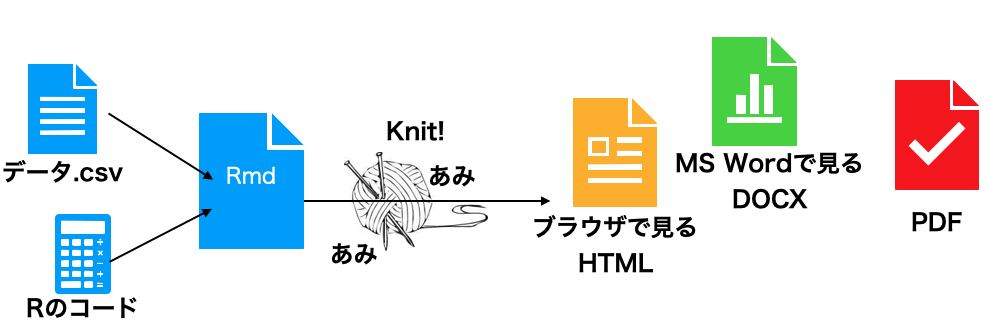
\includegraphics[keepaspectratio]{images/04_RMDknit.png}}

}

\caption{Rmarkdownをknitするイメージ}

\end{figure}%

\begin{figure}[H]

{\centering \pandocbounded{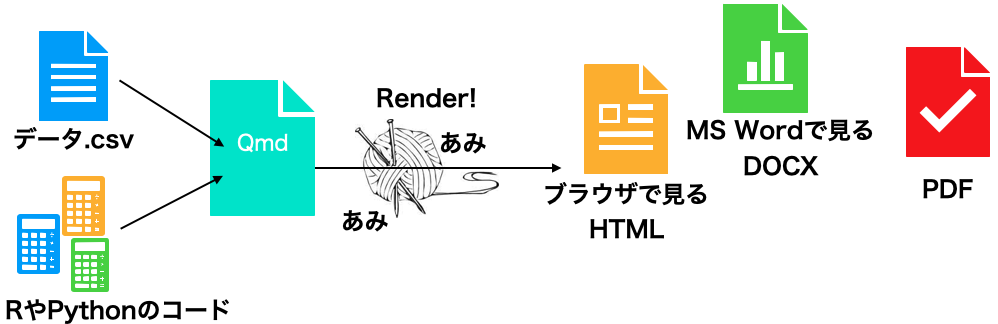
\includegraphics[keepaspectratio]{images/04_QuartoRender.png}}

}

\caption{QuartoファイルをRenderingするイメージ}

\end{figure}%

Quartoも同様に,RStudioのFile \textgreater{} New
Fileから\texttt{Quarto\ Document}を選ぶことで新しいファイル画面が開く。なおRmarkdownファイルの拡張子は\texttt{Rmd}とすることが一般的であり,Quartoは\texttt{Qmd}とすることが一般的である。もっとも,QuartoはRStudio以外のエディタから利用することも考えられていて,例えばVS
Codeなどの一般的なエディタで作成し,コマンドライン経由でコンパイルすることも可能である。

\begin{figure}[H]

{\centering \pandocbounded{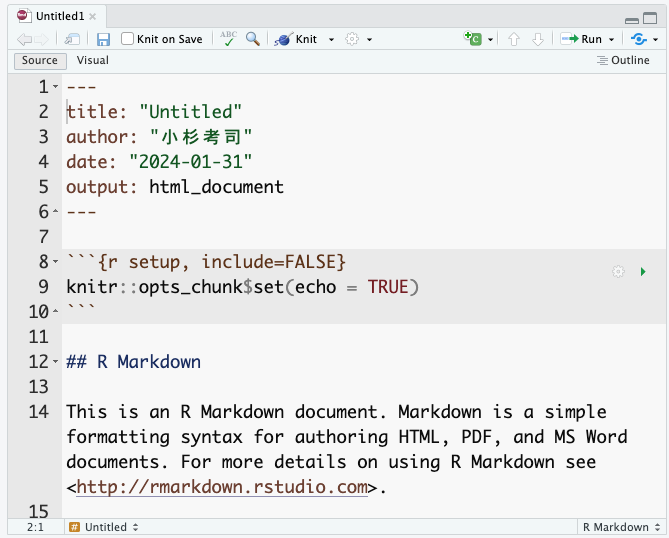
\includegraphics[keepaspectratio]{images/04_RmdSample.png}}

}

\caption{Rmarkdownファイルのサンプル}

\end{figure}%

\begin{figure}[H]

{\centering \pandocbounded{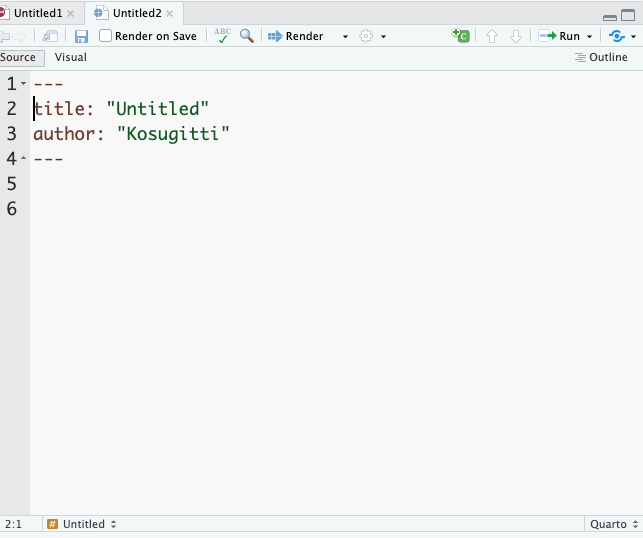
\includegraphics[keepaspectratio]{images/04_QmdSample.png}}

}

\caption{Quartoファイルのサンプル}

\end{figure}%

Rmarkdown,Quartoともに,ファイルの冒頭に4つのハイフンで囲まれた領域が見て取れるだろう。これはYAMLヘッダ(YAMLはYet
Another Markup
Languageの略。ここはまだマークアップ領域じゃないよということ)と呼ばれる,文書全体に対する設定をする領域のことである。

この領域を一瞥すると,タイトルや著者名,出力形式などが記載されていることが見て取れる。YAMLヘッダはインデントに敏感で,また正しくない記述が含まれているとエラーになって出力ファイルが作られないことが少なくないため,ここを手動で書き換えるときは注意が必要である。とはいえ,ここを自在に書き換えることができるようになると,様々な応用が効くので興味があるものは調べて色々トライしてもらいたい。

さて,Rmd/Qmdのファイル上部にKnitあるいはRenderと書かれたボタンがあるだろう。これをクリックすると,表示用ファイルへの変換が実行される。\footnote{もし新しく開いているファイルに名前がつけられていないのなら(Untitledのままになっているようであれば),ファイル名の指定画面が開く。また環境によっては,初回実行時にコンパイルに必要な関連パッケージのダウンロードが求められることがある。}
Rmarkdownの場合は,すでにサンプルコードが含まれているので,数値および図表のはいったHTMLドキュメントが表示されるだろう。以下はこのサンプルコードを例に説明するため,Rmarkdownとそのコンパイル(knit))を一度試してもらいたい。その上で,元のRmdファイルと出来上がったファイルとの対応関係を確認してみよう。

\begin{figure}[H]

{\centering \pandocbounded{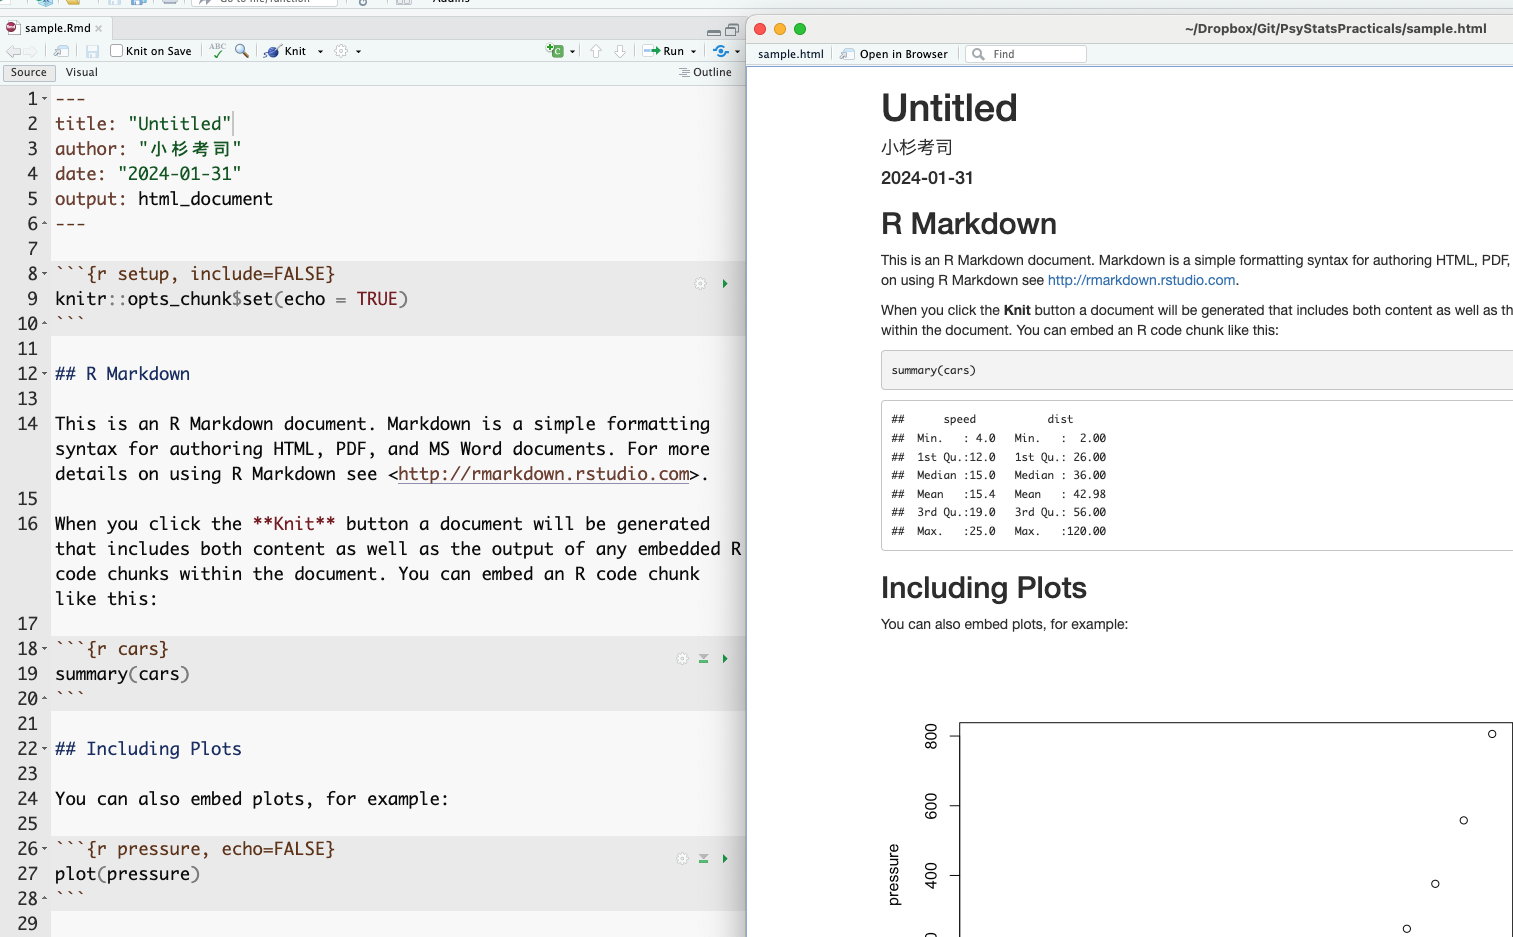
\includegraphics[keepaspectratio]{images/04_coresspRmd.png}}

}

\caption{Rmdファイルと出力結果の対応}

\end{figure}%

おおよそ,何がどのように変換されているかの対応が推察できるだろう。
出力ファイルの冒頭には,YAMLで設定したタイトル,著者名,日付などが表示されているし,\texttt{\#}の印がついていた一行は見出しとして強調されている。

特に注目したいのが,元のファイルで3つのクォーテーションで囲まれた灰色の領域である。この領域のことを特に\textbf{チャンク}といい,ここに書かれたRスクリプトが変換時に実行され,結果として出力される。出力ファイルをみると,\texttt{summary(cars)}
というチャンクで指定された命令文があり,その結果(carsというデータセットの要約)が出力されているのが見て取れる。繰り返しになるが,ポイントは原稿ファイルには計算を指示するスクリプトが書かれているだけで,出力結果を書いていないことにある。原稿は指示だけなのである。こうすることで,コピー&ペーストのミスがなくなるし,同じRmd/Qmd原稿とデータを持っていれば,ことなるPC上でも同じ出力が得られる。環境を統合することで,ミスの防止と再現可能性に貢献しているのがわかるだろう。

今回は\texttt{cars}というRがデフォルトでもっているサンプルデータの例なので,どの環境でも同じ結果が出力されている。しかしもちろん,個別のデータファイルであっても,同じファイルで同じ読み込み方,同じ加工をしていれば,環境が違っても追跡可能である。注意して欲しいのは,コンパイルするときは新しい環境から行われるという点ある。すなわち,\textbf{原稿ファイルにないオブジェクトの利用はできない}のである。これは再現性を担保するという意味では当然のことで,「事前に別途処理しておいたデータ」から分析を始められても,その事前処理が適切だったかどうかがチェックできないからである。Rmd/Qmdファイルと,CSVファイルなどの素データが共有されていれば再現できる,という利点を活かすため,データハンドリングを含めた前処理も全てチャンクに書き込み,新しい環境で最初からトレースできるようにする必要がある。不便に感じるところもあるかもしれないが,科学的営みとして重要な手続きであることを理解してもらいたい。\footnote{もっとも,Rのバージョンやパッケージのバージョンによっては同じ計算結果が出ない可能性がある。より本質的な計算過程に違いがあるかもしれないのである。そのため,R本体やパッケージのバージョンごとパッキングして共有する工夫も考えられている。Dockerと呼ばれるシステムは,解析環境ごと保全し共有するシステムの例である。}

RStudiでは,ビジュアルモードやアウトライン表示,チャンク挿入ボタンやチャンクごとの実行・設定などRmd/Qmdファイルの編集に便利な機能も複数用意されているので,
\textcite{Takahashi201805} などを参考にいろいろ試してみるといいだろう。

\subsection{マークダウンの記法}\label{ux30deux30fcux30afux30c0ux30a6ux30f3ux306eux8a18ux6cd5}

以下では,マークダウン記法について基本的な利用法を解説する。

\subsubsection{見出しと強調}\label{ux898bux51faux3057ux3068ux5f37ux8abf}

すでに見たように,マークダウンでは\texttt{\#}記号で見出しを作ることができる。\texttt{\#}の数が見出しレベルに対応し,\texttt{\#}はトップレベル,本でいうところの「章,chapter」,HTMLでいうところの\texttt{H1}に相当する。\texttt{\#}記号の後ろに半角スペースが必要なことに注意されたし。以下,\texttt{\#\#}で「節,section」あるいは\texttt{H2},\texttt{\#\#\#}で小節(subsection,\texttt{H3}),\texttt{\#\#\#\#}で小小節(subsubsection,\texttt{H4})\ldots と続く。

心理学を始め,科学論文の書き方としての「パラグラフライティング」を既にみしっていることだろう。文章をセクション,サブセクション,パラグラフ,センテンスのように階層的に分割し,それぞれの区分が4つの下位区分を含むような文章構造である。心理学の場合は特に「問題,方法,結果,考察」の4セクションで一論文が構成されるのが基本である。こうしたアウトラインを意識した書き方は読み手にも優しく,マークダウンの記法ではそれが自然と実装できるようになっている。

これとは別に,一部を太字や斜体で強調したいこともあるだろう。そのような場合はアスタリスクを1つ,あるいは2つつけて\emph{強調}したり\textbf{強調}したりできる。

\subsubsection{図表とリンク}\label{ux56f3ux8868ux3068ux30eaux30f3ux30af}

文中に図表を挿入したいこともあるだろう。表の挿入は,マークダウン独自の記法があり,縦棒\texttt{\textbar{}}やハイフン\texttt{-}を駆使して以下のように表記する。

\begin{verbatim}
| Header 1 | Header 2 | Header 3 |
| -------- | -------- | -------- |
| Row 1    | Data 1   | Data 2   |
| Row 2    | Data 3   | Data 4   |
\end{verbatim}

Rのコードの中には分析結果をマークダウン形式で出力してくれる関数もあるし,表計算ソフトなどでできた表があるなら,chatGPTなど生成AIを利用するとすぐに書式変換してくれるので,そういったツールを活用すると良い。

図の挿入は,マークダウンでは図のファイルへのリンクと考えると良い。次のように,大括弧で括った文字がキャプション,つづく小括弧で括ったものが図へのリンクとなる。実際に表示されるときは図が示される。

\begin{verbatim}
![図のキャプション](図へのリンク)
\end{verbatim}

同様に,ウェブサイトへのリンクなども,\texttt{{[}表示名{]}(リンク先)}の書式で対応できる。

\subsubsection{リスト}\label{ux30eaux30b9ux30c8}

並列的に箇条書きを示したい場合は,プラスあるいはマイナスでリストアップする。注意すべきは,リストの前後に改行を入れておくべきことである。

\begin{verbatim}
ここまで前の文

+  list item 1
+  list item 2
+  list item 3
    - sub item 1
    - sub item 2

ここから次の文
\end{verbatim}

\subsubsection{チャンク}\label{ux30c1ux30e3ux30f3ux30af}

既に述べたように,チャンク(chunk)と呼ばれる領域は実行されるコードを記載するところである。チャンクはまず,バックスラッシュ3つ繋げることでコードブロックであることを示し,次に
\texttt{r}と書くことで計算エンジンがRであることを明示する。ここにJuiliaやPythonなど他の計算エンジンを指定することも可能である。

可能であれば,チャンク名をつけておくと良い。次の例は,チャンク名として「chunksample」を与えたものである。チャンク名をつけておくと,RStudioでは見出しジャンプをつかって移動することもできるので,編集時に便利である。

```\{r chunksample,echo = FALSE\} summary(cars) ```

さらに,\texttt{echo\ =\ FALSE}のようにチャンクオプションを指定することができる。\texttt{echo=FALSE}は入力したスクリプトを表示せず,結果だけにするオプションである。そのほか「計算結果を含めない」「表示せずに計算は実行する」等様々な指定が可能である。

なおQuartoではこのチャンクオプションを次のように書くこともできる。

```\{r\} \#\textbar{} echo: FALSE \#\textbar{} include: FALSE
summary(cars) ```

\section{プロットによる基本的な描画}\label{ux30d7ux30edux30c3ux30c8ux306bux3088ux308bux57faux672cux7684ux306aux63cfux753b}

再現可能な文書という観点から,図表もスクリプトによる記述で表現することは重要である。

\textbf{データはまず可視化するもの}と心がけよ。可視化は,数値の羅列あるいはまとめられた統計量では把握しきれない多くの情報を提供し,潜在的な関係性を直観的に見つけ出せる可能性がある。なので,取得したあらゆる\textbf{データはまず可視化するもの},と思っておいて間違いはない。大事なことなので二度言いました。可視化の重要性については心理学の知見にも触れている
\textcite{Kieran2018} も参考にしてほしい。

さて,Rには基本的な作図環境も整っており,\texttt{plot}という関数に引数として,x軸,y軸に相当する変数を与えるだけで,簡単に散布図を書いてくれる。

\begin{Shaded}
\begin{Highlighting}[]
\FunctionTok{plot}\NormalTok{(iris}\SpecialCharTok{$}\NormalTok{Sepal.Length, iris}\SpecialCharTok{$}\NormalTok{Sepal.Width,}
  \AttributeTok{main =} \StringTok{"Example of Scatter Plot"}\NormalTok{,}
  \AttributeTok{xlab =} \StringTok{"Sepal.Length"}\NormalTok{,}
  \AttributeTok{ylab =} \StringTok{"Sepal.Width"}
\NormalTok{)}
\end{Highlighting}
\end{Shaded}

\pandocbounded{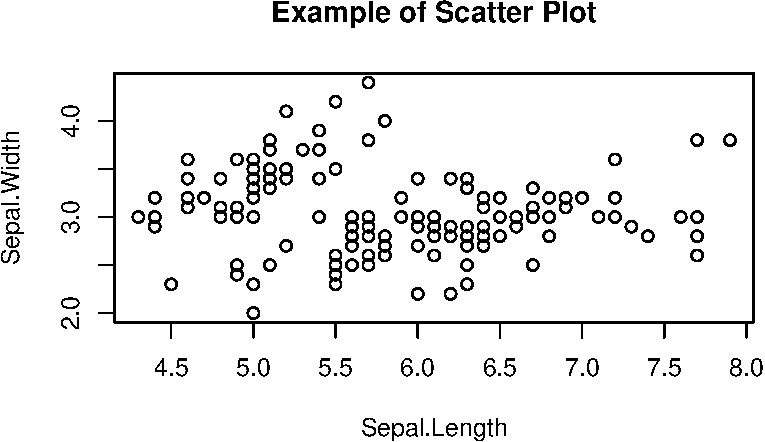
\includegraphics[keepaspectratio]{chapter04_files/figure-pdf/RplotSample-1.pdf}}

この関数のオプションとして,タイトルを与えたり,軸に名前を与えたりできる。またプロットされるピンの形,描画色,背景色など様々な操作が可能である。特段のパッケージを必要とせずとも,基本的な描画機能は備えていると言えるだろう。

\section{ggplotによる描画}\label{ggplotux306bux3088ux308bux63cfux753b}

ここでは,\texttt{tidyverse}に含まれる描画専用のパッケージである,\texttt{ggplot2}
パッケージを用いた描画を学ぶ。Rの基本描画関数でもかなりのことができるのだが,この\texttt{ggplot2}パッケージをもちいた図の方が美しく,直観的に操作できる。というのも\texttt{ggplot}の\texttt{gg}とは\texttt{The\ Grammar\ of\ Graphics}(描画の文法)のことであり,このことが示すようにロジカルに図版を制御できるからである。\texttt{ggplot2}の形で記述された図版のスクリプトは可読性が高く,視覚的にも美しいため,多くの文献で利用されている。

\texttt{ggplot2}
パッケージの提供する描画環境の特徴は,レイア(Layer)の概念である。図版は複数のレイアの積み重ねとして表現される。まず土台となるキャンバスがあり,そこにデータセット,幾何学的オブジェクト(点,線,バーなど),エステティックマッピング(色,形,サイズなど),凡例やキャプションを重ねていく,という発想である。そして図版全体を通したテーマを手強することで,カラーパレットの統一などの仕上げをすれば,すぐにでも論文投稿可能なレベルの図版を描くことができる。

以下に\texttt{ggplot2}における描画のサンプルを示す。サンプルデータ\texttt{mtcars}を用いた。

\begin{Shaded}
\begin{Highlighting}[]
\NormalTok{pacman}\SpecialCharTok{::}\FunctionTok{p\_load}\NormalTok{(ggplot2)}

\FunctionTok{ggplot}\NormalTok{(}\AttributeTok{data =}\NormalTok{ mtcars, }\FunctionTok{aes}\NormalTok{(}\AttributeTok{x =}\NormalTok{ wt, }\AttributeTok{y =}\NormalTok{ mpg)) }\SpecialCharTok{+}
  \FunctionTok{geom\_point}\NormalTok{() }\SpecialCharTok{+}
  \FunctionTok{geom\_smooth}\NormalTok{(}\AttributeTok{method =} \StringTok{"lm"}\NormalTok{, }\AttributeTok{formula =} \StringTok{"y \textasciitilde{} x"}\NormalTok{) }\SpecialCharTok{+}
  \FunctionTok{labs}\NormalTok{(}\AttributeTok{title =} \StringTok{"車の重量と燃費の関係"}\NormalTok{, }\AttributeTok{x =} \StringTok{"重量"}\NormalTok{, }\AttributeTok{y =} \StringTok{"燃費"}\NormalTok{)}
\end{Highlighting}
\end{Shaded}

\pandocbounded{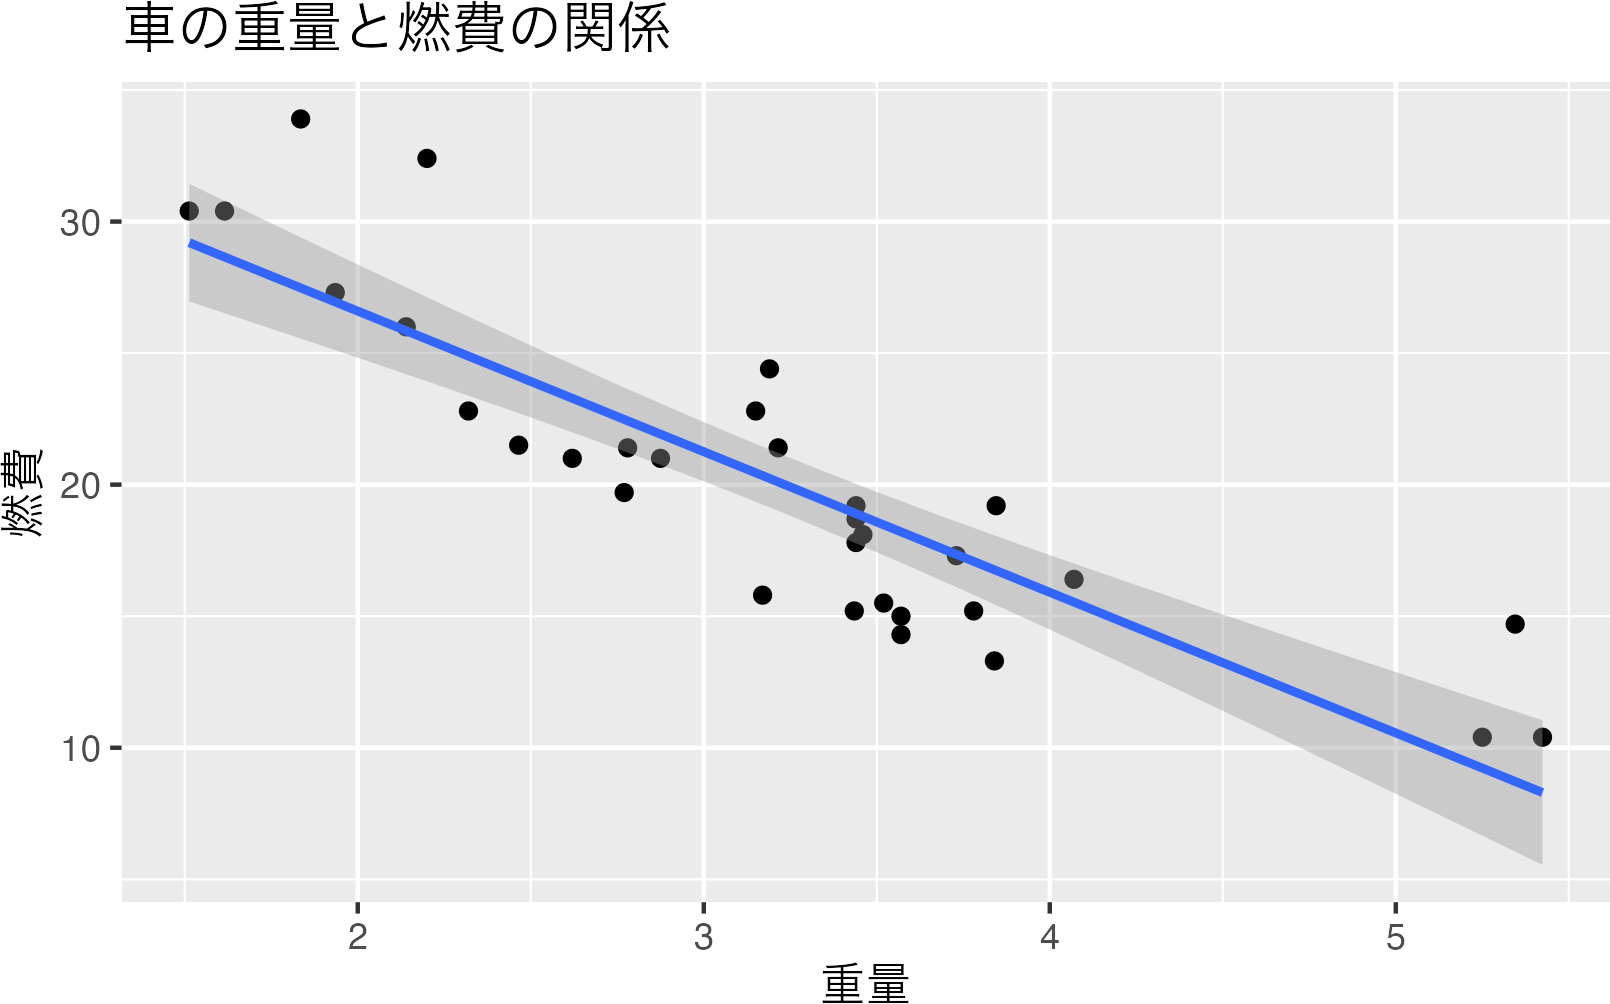
\includegraphics[keepaspectratio]{chapter04_files/figure-pdf/ggplotSample1-1.png}}

まずは出来上がる図版の美しさと,コードのイメージを把握してもらいたい。
最初の\texttt{pacman::p\_load(ggplot2)}はパッケージを読み込んでいるところである。今回は明示的に\texttt{ggplot2}を読み込んでいるが,\texttt{tidyverse}パッケージを読み込むと同時に読み込まれているので,Rのスクリプトの冒頭に\texttt{pacman::p\_load(tidyverse)}と書く癖をつけておけば必要ない。

続いて\texttt{ggplot}の関数が4行にわたって書いてあるが,それぞれが\texttt{+}の記号で繋がれていることがわかるだろう。これがレイアを重ねるという作業に相当する。まずは,図を書くためのキャンバスを用意し,その上にいろいろ重ねていくのである。

次のコードは,キャンバスだけを描画した例である。

\begin{Shaded}
\begin{Highlighting}[]
\NormalTok{g }\OtherTok{\textless{}{-}} \FunctionTok{ggplot}\NormalTok{()}
\FunctionTok{print}\NormalTok{(g)}
\end{Highlighting}
\end{Shaded}

\pandocbounded{
\includegraphics[keepaspectratio]{chapter04_files/figure-pdf/canvasOnly-1.pdf}}

ここでは\texttt{g}
というオブジェクトを\texttt{ggplot}関数でつくり,それを表示させた。最初はこのようにプレーンなキャンバスだが,ここに次々と上書きしていくことになる。

\section{幾何学的オブジェクトgeom}\label{ux5e7eux4f55ux5b66ux7684ux30aaux30d6ux30b8ux30a7ux30afux30c8geom}

幾何学的オブジェクト(geometric object)
とは,データの表現方法の指定であり,\texttt{ggplot}には様々なパターンが用意されている。以下に一例を挙げる。

\begin{itemize}
\tightlist
\item
  \textbf{\texttt{geom\_point()}}:
  散布図で使用され、データ点を個々の点としてプロットする。
\item
  \textbf{\texttt{geom\_line()}}:
  折れ線グラフで使用され、データ点を線で結んでプロットする。時系列データなどによく使われる。
\item
  \textbf{\texttt{geom\_bar()}}:
  棒グラフで使用され、カテゴリごとの量を棒で表示する。データの集計(カウントや合計など)に適している。
\item
  \textbf{\texttt{geom\_histogram()}}:
  ヒストグラムで使用され、連続データの分布を棒で表示する。データの分布を理解するのに役立つ。
\item
  \textbf{\texttt{geom\_boxplot()}}:
  箱ひげ図で使用され、データの分布(中央値、四分位数、外れ値など)を要約して表示する。
\item
  \textbf{\texttt{geom\_smooth()}}:
  平滑化曲線を追加し、データのトレンドやパターンを可視化する。線形回帰やローパスフィルタなどの方法が使われる。
\end{itemize}

これらの幾何学的オブジェクトに,データおよび軸との対応を指定するなどして描画する。次に挙げるのは\texttt{geom\_point}
による点描画,つまり散布図である。

\begin{Shaded}
\begin{Highlighting}[]
\FunctionTok{ggplot}\NormalTok{() }\SpecialCharTok{+}
  \FunctionTok{geom\_point}\NormalTok{(}\AttributeTok{data =}\NormalTok{ mtcars, }\AttributeTok{mapping =} \FunctionTok{aes}\NormalTok{(}\AttributeTok{x =}\NormalTok{ disp, }\AttributeTok{y =}\NormalTok{ wt))}
\end{Highlighting}
\end{Shaded}

\pandocbounded{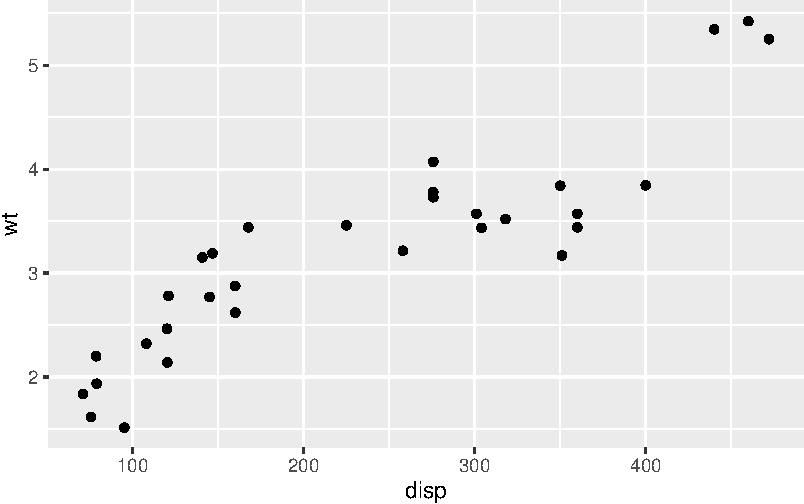
\includegraphics[keepaspectratio]{chapter04_files/figure-pdf/geom_exam-1.pdf}}

一行目でキャンバスを用意し,そこに\texttt{geom\_point}で点を打つようにしている。
このとき,データは\texttt{mtcars}であり,x軸に変数\texttt{disp}を,y軸に変数\texttt{wt}をマッピングしている。マッピング関数の\texttt{aes}はaesthetic
mappingsの意味で,データによって変わる値(x座標,y座標,色,サイズ,透明度など)を指定することができる。

レイアは次々と重ねることができる。以下の例を見てみよう。

\begin{Shaded}
\begin{Highlighting}[]
\NormalTok{g }\OtherTok{\textless{}{-}} \FunctionTok{ggplot}\NormalTok{()}
\NormalTok{g1 }\OtherTok{\textless{}{-}}\NormalTok{ g }\SpecialCharTok{+} \FunctionTok{geom\_point}\NormalTok{(}\AttributeTok{data =}\NormalTok{ mtcars, }\AttributeTok{mapping =} \FunctionTok{aes}\NormalTok{(}\AttributeTok{x =}\NormalTok{ disp, }\AttributeTok{y =}\NormalTok{ wt))}
\NormalTok{g2 }\OtherTok{\textless{}{-}}\NormalTok{ g1 }\SpecialCharTok{+} \FunctionTok{geom\_line}\NormalTok{(}\AttributeTok{data =}\NormalTok{ mtcars, }\AttributeTok{mapping =} \FunctionTok{aes}\NormalTok{(}\AttributeTok{x =}\NormalTok{ disp, }\AttributeTok{y =}\NormalTok{ wt))}
\FunctionTok{print}\NormalTok{(g2)}
\end{Highlighting}
\end{Shaded}

\pandocbounded{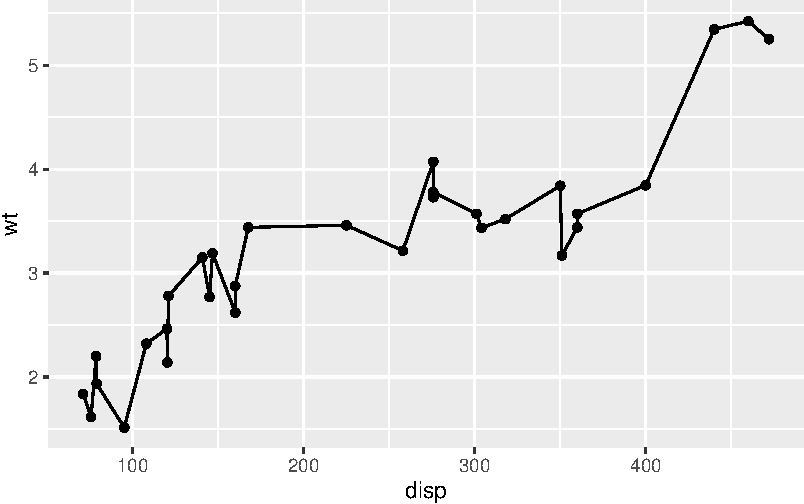
\includegraphics[keepaspectratio]{chapter04_files/figure-pdf/geom_overlay-1.pdf}}

重ねることを強調するために,\texttt{g}
オブジェクトを次々作るようにしたが,もちろん1つのオブジェクトでまとめて書いてもいいし,\texttt{g}オブジェクトとして保管せずとも,最初の例のように直接出力することもできる。また,ここでは点描画オブジェクトに線描画オブジェクトを重ねているが,データやマッピングは全く同じである。異なるデータを一枚のキャンバスに書く場合は,このように幾何学オブジェクトごとの指定が可能であるが,図版は得てして一枚のキャンバスに一種類のデータになりがちである。そのような場合は,以下に示すようにキャンバスの段階から基本となるデータセットとマッピングを与えることが可能である。

\begin{Shaded}
\begin{Highlighting}[]
\FunctionTok{ggplot}\NormalTok{(}\AttributeTok{data =}\NormalTok{ mtcars, }\AttributeTok{mapping =} \FunctionTok{aes}\NormalTok{(}\AttributeTok{x =}\NormalTok{ disp, }\AttributeTok{y =}\NormalTok{ wt)) }\SpecialCharTok{+}
  \FunctionTok{geom\_point}\NormalTok{() }\SpecialCharTok{+}
  \FunctionTok{geom\_line}\NormalTok{()}
\end{Highlighting}
\end{Shaded}

また,この用例の場合\texttt{ggplot}関数の第一引数はデータセットなので,パイプ演算子で渡すことができる。

\begin{Shaded}
\begin{Highlighting}[]
\NormalTok{mtcars }\SpecialCharTok{\%\textgreater{}\%}
  \FunctionTok{ggplot}\NormalTok{(}\AttributeTok{mapping =} \FunctionTok{aes}\NormalTok{(}\AttributeTok{x =}\NormalTok{ disp, }\AttributeTok{y =}\NormalTok{ wt)) }\SpecialCharTok{+}
  \FunctionTok{geom\_point}\NormalTok{() }\SpecialCharTok{+}
  \FunctionTok{geom\_line}\NormalTok{()}
\end{Highlighting}
\end{Shaded}

パイプ演算子を使うことで,素データをハンドリングし,必要な形に整えて可視化する,という流れがスクリプト上で読むように表現できるようになる。慣れてくると,データセットから可視化したい要素を特定し,最終的にどのように成形すれば\texttt{ggplot}に渡しやすくなるかを想像して加工していくようになる。そのためには到達目標となる図版のイメージを頭に描き,その図のx軸,y軸は何で,どのような幾何学オブジェクトが上に乗っているのか,といったように図版のリバースエンジニアリング,あるいは図版の作成手順の書き下しができる必要がある。たとえるなら,食べたい料理に必要な材料を集め,大まかな手順(下ごしらえからの調理)を組み立てられるかどうか,である。実際にレシピに書き起こす際は生成AIの力を借りると良いが,その際も最終的な目標と,全体的な設計方針から指示し,微調整を追加していくように指示すると効率的である。

以下に,データハンドリングと描画の一例を示す。各ステップにコメントをつけたので,文章を読むように加工と描画の流れを確認し,出力結果と照らし合わせてみよう。

\begin{Shaded}
\begin{Highlighting}[]
\CommentTok{\# mtcarsデータセットを使用}
\NormalTok{mtcars }\SpecialCharTok{\%\textgreater{}\%}
  \CommentTok{\# 変数選択}
  \FunctionTok{select}\NormalTok{(mpg, cyl, wt, am) }\SpecialCharTok{\%\textgreater{}\%}
  \FunctionTok{mutate}\NormalTok{(}
    \CommentTok{\# 変数am,cylをFactor型に変換}
    \AttributeTok{am =} \FunctionTok{factor}\NormalTok{(am, }\AttributeTok{labels =} \FunctionTok{c}\NormalTok{(}\StringTok{"automatic"}\NormalTok{, }\StringTok{"manual"}\NormalTok{)),}
    \AttributeTok{cyl =} \FunctionTok{factor}\NormalTok{(cyl)}
\NormalTok{  ) }\SpecialCharTok{\%\textgreater{}\%}
  \CommentTok{\# 水準ごとにグループ化}
  \FunctionTok{group\_by}\NormalTok{(am, cyl) }\SpecialCharTok{\%\textgreater{}\%}
  \FunctionTok{summarise}\NormalTok{(}
    \AttributeTok{M =} \FunctionTok{mean}\NormalTok{(mpg), }\CommentTok{\# 各グループの平均燃費(M)を計算}
    \AttributeTok{SD =} \FunctionTok{sd}\NormalTok{(mpg), }\CommentTok{\# 各グループの燃費の標準偏差(SD)を計算}
    \AttributeTok{.groups =} \StringTok{"drop"} \CommentTok{\# summarise後の自動的なグルーピングを解除}
\NormalTok{  ) }\SpecialCharTok{\%\textgreater{}\%}
  \CommentTok{\# x軸にトランスミッションの種類、y軸に平均燃費,塗りつぶしの色はcyl}
  \FunctionTok{ggplot}\NormalTok{(}\FunctionTok{aes}\NormalTok{(}\AttributeTok{x =}\NormalTok{ am, }\AttributeTok{y =}\NormalTok{ M, }\AttributeTok{fill =}\NormalTok{ cyl)) }\SpecialCharTok{+}
  \CommentTok{\# 横並びの棒グラフ}
  \FunctionTok{geom\_bar}\NormalTok{(}\AttributeTok{stat =} \StringTok{"identity"}\NormalTok{, }\AttributeTok{position =} \StringTok{"dodge"}\NormalTok{) }\SpecialCharTok{+}
  \CommentTok{\# ±1SDのエラーバーを追加}
  \FunctionTok{geom\_errorbar}\NormalTok{(}
    \CommentTok{\# エラーバーのマッピング}
    \FunctionTok{aes}\NormalTok{(}\AttributeTok{ymin =}\NormalTok{ M }\SpecialCharTok{{-}}\NormalTok{ SD, }\AttributeTok{ymax =}\NormalTok{ M }\SpecialCharTok{+}\NormalTok{ SD),}
    \CommentTok{\# エラーバーの位置を棒グラフに合わせる}
    \AttributeTok{position =} \FunctionTok{position\_dodge}\NormalTok{(}\AttributeTok{width =} \FloatTok{0.9}\NormalTok{),}
    \AttributeTok{width =} \FloatTok{0.25} \CommentTok{\# エラーバーの幅を設定}
\NormalTok{  )}
\end{Highlighting}
\end{Shaded}

\pandocbounded{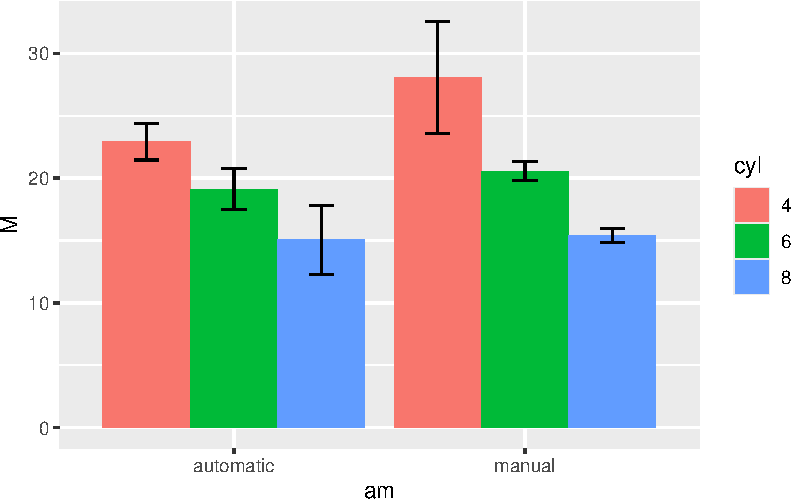
\includegraphics[keepaspectratio]{chapter04_files/figure-pdf/withHandlingGGplot-1.pdf}}

繰り返しになるが,このコードは慣れてくるまでいきなり書けるものではない。重要なのは「出力結果をイメージ」することと,それを「要素に分解」,「手順に沿って並べる」ことができるかどうかである。\footnote{実際コードはchatGPTver4に指示して生成した。いきなり全体像を描くのではなく,徐々に追記していくと効果的である。}

\section{描画tips}\label{ux63cfux753btips}

最後に,いくつかの描画テクニックを述べておく。これらについては,必要な時に随時ウェブ上で検索したり,生成AIに尋ねることでも良いが,このような方法がある,という基礎知識を持っておくことも重要だろう。なお描画について詳しくは
\textcite{Kinosady2021} の4章を参照すると良い。

\subsection{ggplotオブジェクトを並べる}\label{ggplotux30aaux30d6ux30b8ux30a7ux30afux30c8ux3092ux4e26ux3079ux308b}

複数のプロットを一枚のパネルに配置したい,ということがあるかもしれない。先ほどの\texttt{mtcars}データの例でいえば,\texttt{am}変数にオートマチック車かマニュアル車かの2水準があるが,このようなサブグループごとに図を分割したいという場合である。

このような時には,\texttt{facet\_wrap}や\texttt{facet\_grid}という関数が便利である。前者はある変数について,後者は2つの変数について図を分割する。

\begin{Shaded}
\begin{Highlighting}[]
\NormalTok{mtcars }\SpecialCharTok{\%\textgreater{}\%}
  \CommentTok{\# 重さwtと燃費mpgの散布図}
  \FunctionTok{ggplot}\NormalTok{(}\FunctionTok{aes}\NormalTok{(}\AttributeTok{x =}\NormalTok{ wt, }\AttributeTok{y =}\NormalTok{ mpg)) }\SpecialCharTok{+}
  \FunctionTok{geom\_point}\NormalTok{() }\SpecialCharTok{+}
  \CommentTok{\# シリンダ数cylで分割}
  \FunctionTok{facet\_wrap}\NormalTok{(}\SpecialCharTok{\textasciitilde{}}\NormalTok{cyl, }\AttributeTok{nrow =} \DecValTok{2}\NormalTok{) }\SpecialCharTok{+}
  \CommentTok{\# タイトルをつける}
  \FunctionTok{labs}\NormalTok{(}\AttributeTok{caption =} \StringTok{"facet\_wrapの例"}\NormalTok{)}
\end{Highlighting}
\end{Shaded}

\pandocbounded{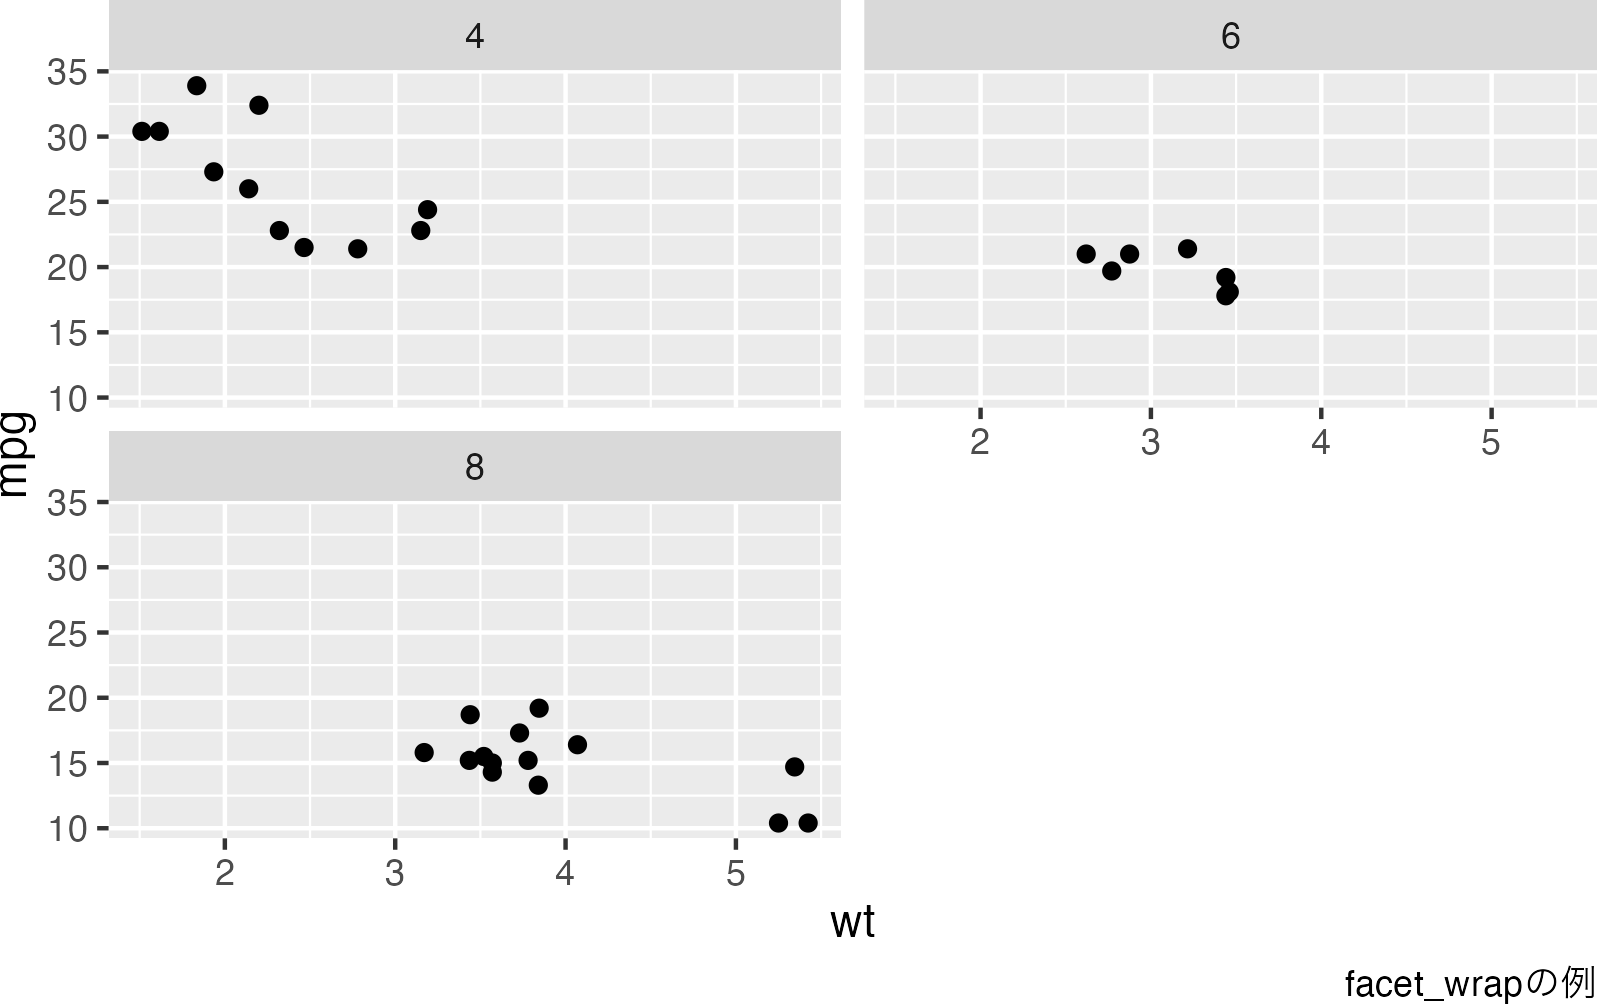
\includegraphics[keepaspectratio]{chapter04_files/figure-pdf/exampleFacetWrap-1.png}}

\begin{Shaded}
\begin{Highlighting}[]
\NormalTok{mtcars }\SpecialCharTok{\%\textgreater{}\%}
  \FunctionTok{ggplot}\NormalTok{(}\FunctionTok{aes}\NormalTok{(}\AttributeTok{x =}\NormalTok{ wt, }\AttributeTok{y =}\NormalTok{ mpg)) }\SpecialCharTok{+}
  \FunctionTok{geom\_point}\NormalTok{() }\SpecialCharTok{+}
  \CommentTok{\# シリンダ数cylとギア数gearで分割}
  \FunctionTok{facet\_grid}\NormalTok{(cyl }\SpecialCharTok{\textasciitilde{}}\NormalTok{ gear) }\SpecialCharTok{+}
  \CommentTok{\# キャプションをつける}
  \FunctionTok{labs}\NormalTok{(}\AttributeTok{caption =} \StringTok{"facet\_gridの例"}\NormalTok{)}
\end{Highlighting}
\end{Shaded}

\pandocbounded{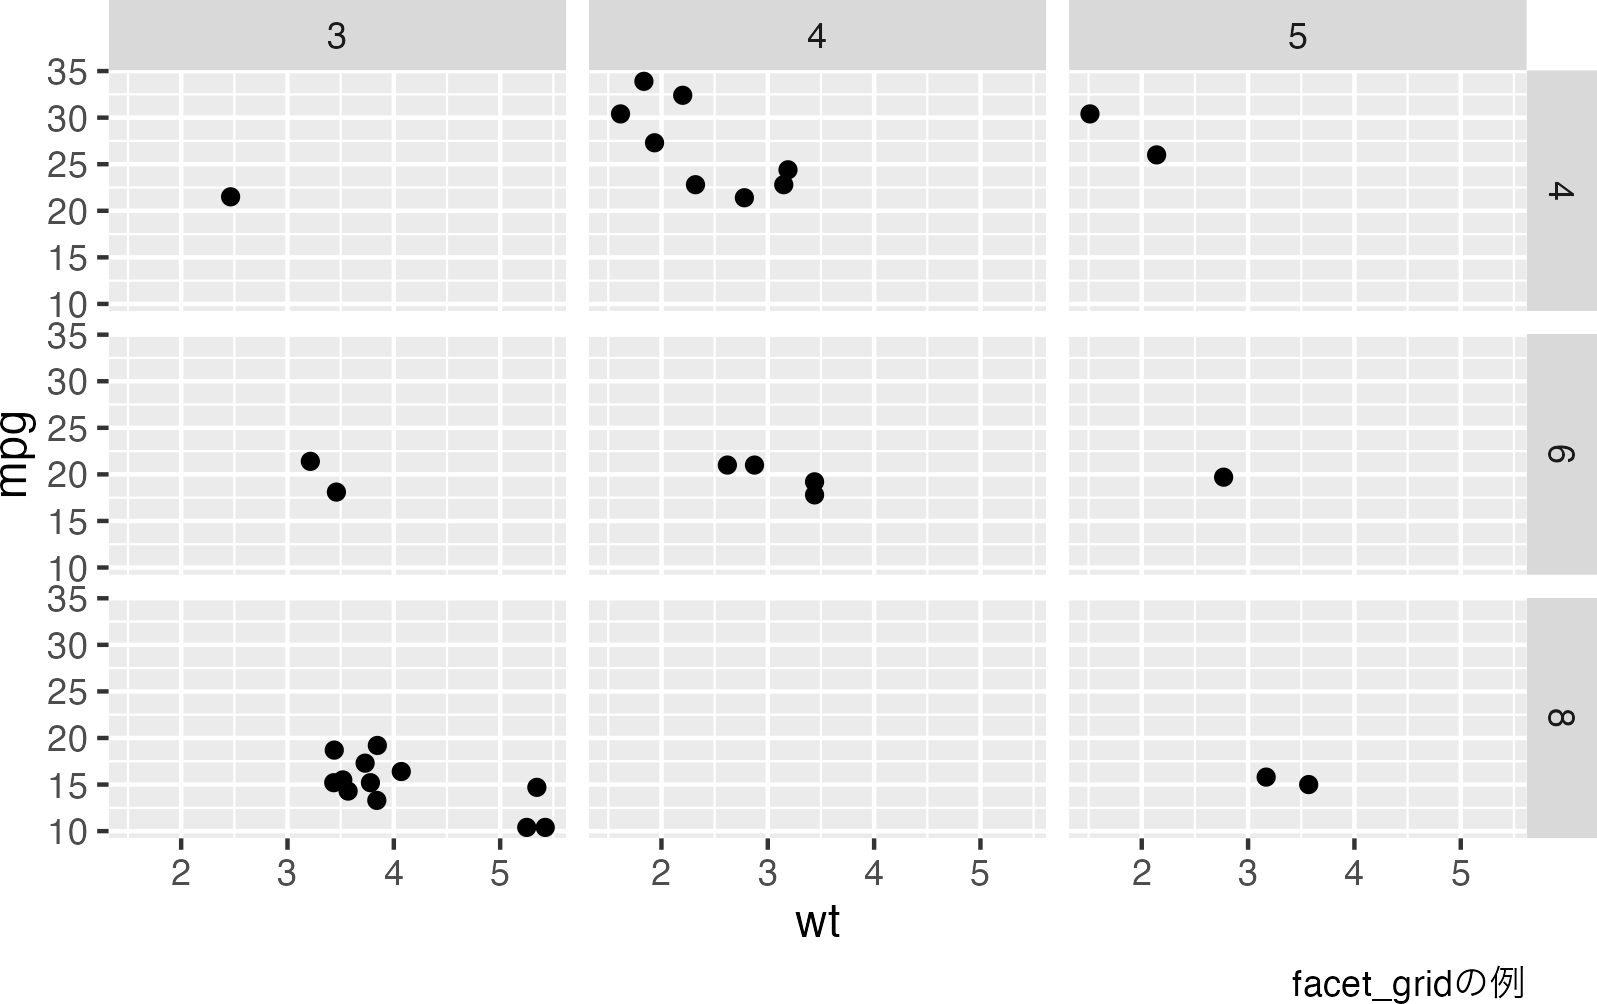
\includegraphics[keepaspectratio]{chapter04_files/figure-pdf/exampleFacetGrid-1.png}}

一枚の図をサブグループに分けるのではなく,異なる図を一枚の図として赤痛いこともあるかもしれない。そのような場合は,\texttt{patchwork}パッケージを使うと便利である。

\begin{Shaded}
\begin{Highlighting}[]
\NormalTok{pacman}\SpecialCharTok{::}\FunctionTok{p\_load}\NormalTok{(patchwork)}

\CommentTok{\# 散布図の作成}
\NormalTok{g1 }\OtherTok{\textless{}{-}} \FunctionTok{ggplot}\NormalTok{(mtcars, }\FunctionTok{aes}\NormalTok{(}\AttributeTok{x =}\NormalTok{ wt, }\AttributeTok{y =}\NormalTok{ mpg)) }\SpecialCharTok{+}
  \FunctionTok{geom\_point}\NormalTok{() }\SpecialCharTok{+}
  \CommentTok{\# 散布図のタイトルとサブタイトル}
  \FunctionTok{ggtitle}\NormalTok{(}\StringTok{"Scatter Plot"}\NormalTok{, }\StringTok{"MPG vs Weight"}\NormalTok{)}

\CommentTok{\# 棒グラフの作成}
\NormalTok{g2 }\OtherTok{\textless{}{-}} \FunctionTok{ggplot}\NormalTok{(mtcars, }\FunctionTok{aes}\NormalTok{(}\AttributeTok{x =} \FunctionTok{factor}\NormalTok{(cyl), }\AttributeTok{y =}\NormalTok{ mpg)) }\SpecialCharTok{+}
  \FunctionTok{geom\_bar}\NormalTok{(}\AttributeTok{stat =} \StringTok{"identity"}\NormalTok{) }\SpecialCharTok{+}
  \CommentTok{\# 棒グラフのタイトルとサブタイトル}
  \FunctionTok{ggtitle}\NormalTok{(}\StringTok{"Bar Chart"}\NormalTok{, }\StringTok{"Average MPG by Cylinder"}\NormalTok{)}

\CommentTok{\# patchworkを使用して2つのグラフを組み合わせる}
\NormalTok{combined\_plot }\OtherTok{\textless{}{-}}\NormalTok{ g1 }\SpecialCharTok{+}\NormalTok{ g2 }\SpecialCharTok{+}
  \FunctionTok{plot\_annotation}\NormalTok{(}
    \AttributeTok{title =} \StringTok{"Combined Plots"}\NormalTok{,}
    \AttributeTok{subtitle =} \StringTok{"Scatter and Bar Charts"}
\NormalTok{  )}

\CommentTok{\# プロットを表示}
\FunctionTok{print}\NormalTok{(combined\_plot)}
\end{Highlighting}
\end{Shaded}

\pandocbounded{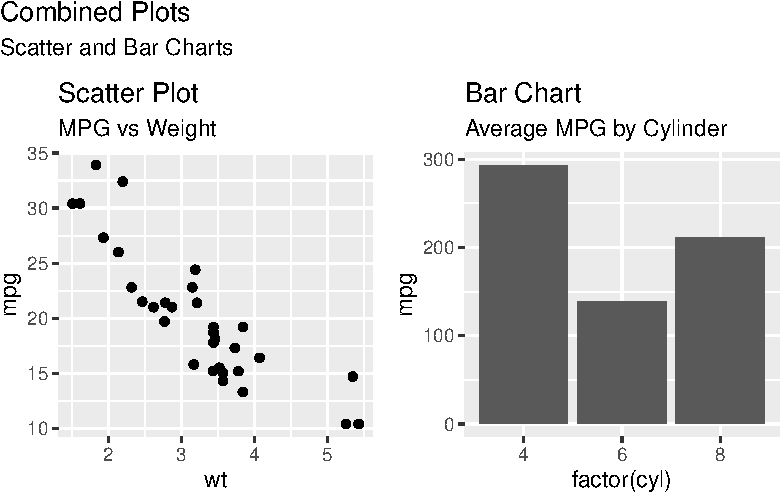
\includegraphics[keepaspectratio]{chapter04_files/figure-pdf/patchwork example-1.pdf}}

\subsection{ggplotオブジェクトの保存}\label{ggplotux30aaux30d6ux30b8ux30a7ux30afux30c8ux306eux4fddux5b58}

RmdやQuartoで文書を作るときは,図が自動的に生成されるので問題ないが,図だけ別のファイルとして利用したい,保存したいということがあるかもしれない。その時は\texttt{ggsave}関数で\texttt{ggplot}オブジェクトを保存するとよい。

\begin{Shaded}
\begin{Highlighting}[]
\CommentTok{\# 散布図を作成}
\NormalTok{p }\OtherTok{\textless{}{-}} \FunctionTok{ggplot}\NormalTok{(mtcars, }\FunctionTok{aes}\NormalTok{(}\AttributeTok{x =}\NormalTok{ wt, }\AttributeTok{y =}\NormalTok{ mpg)) }\SpecialCharTok{+}
  \FunctionTok{geom\_point}\NormalTok{()}
\FunctionTok{ggsave}\NormalTok{(}
  \AttributeTok{filename =} \StringTok{"my\_plot.png"}\NormalTok{, }\CommentTok{\# 保存するファイル名。}
  \AttributeTok{plot =}\NormalTok{ p, }\CommentTok{\# 保存するプロットオブジェクト。}
  \AttributeTok{device =} \StringTok{"png"}\NormalTok{, }\CommentTok{\# 保存するファイル形式。}
  \AttributeTok{path =} \StringTok{"path/to/directory"}\NormalTok{, }\CommentTok{\# ファイルを保存するディレクトリのパス}
  \AttributeTok{scale =} \DecValTok{1}\NormalTok{, }\CommentTok{\# グラフィックスの拡大縮小比率}
  \AttributeTok{width =} \DecValTok{5}\NormalTok{, }\CommentTok{\# 保存するプロットの幅(インチ)}
  \AttributeTok{height =} \DecValTok{5}\NormalTok{, }\CommentTok{\# 保存するプロットの高さ(インチ)}
  \AttributeTok{dpi =} \DecValTok{300}\NormalTok{, }\CommentTok{\# 解像度(DPI: dots per inch)}
\NormalTok{)}
\end{Highlighting}
\end{Shaded}

\subsection{テーマの変更(レポートに合わせる)}\label{ux30c6ux30fcux30deux306eux5909ux66f4ux30ecux30ddux30fcux30c8ux306bux5408ux308fux305bux308b}

レポートや論文などの提出次の条件として,図版をモノクロで表現しなければならないことがあるかもしれない。\texttt{ggplot}では自動的に配色されるが,その背後ではデフォルトの絵の具セット(\textbf{パレット}という)
が選択されているからである。このセットを変更すると,同じプロットでも異なる配色で出力される。モノクロ(グレイスケール)で出力したい時のパレットは\texttt{Grays}である。

\begin{Shaded}
\begin{Highlighting}[]
\CommentTok{\# グレースケールのプロット}
\NormalTok{p1 }\OtherTok{\textless{}{-}} \FunctionTok{ggplot}\NormalTok{(mtcars, }\FunctionTok{aes}\NormalTok{(}\AttributeTok{x =}\NormalTok{ wt, }\AttributeTok{y =}\NormalTok{ mpg, }\AttributeTok{color =} \FunctionTok{factor}\NormalTok{(cyl))) }\SpecialCharTok{+}
  \FunctionTok{geom\_point}\NormalTok{(}\AttributeTok{size =} \DecValTok{3}\NormalTok{) }\SpecialCharTok{+}
  \FunctionTok{scale\_fill\_brewer}\NormalTok{(}\AttributeTok{palette =} \StringTok{"Greys"}\NormalTok{) }\SpecialCharTok{+}
  \FunctionTok{ggtitle}\NormalTok{(}\StringTok{"Gray Palette"}\NormalTok{)}

\CommentTok{\# カラーパレットが多く含まれているパッケージの利用}
\NormalTok{pacman}\SpecialCharTok{::}\FunctionTok{p\_load}\NormalTok{(RColorBrewer)}
\CommentTok{\# 色覚特性を考慮したカラーパレット}
\NormalTok{p2 }\OtherTok{\textless{}{-}} \FunctionTok{ggplot}\NormalTok{(mtcars, }\FunctionTok{aes}\NormalTok{(}\AttributeTok{x =}\NormalTok{ wt, }\AttributeTok{y =}\NormalTok{ mpg, }\AttributeTok{color =} \FunctionTok{factor}\NormalTok{(cyl))) }\SpecialCharTok{+}
  \FunctionTok{geom\_point}\NormalTok{(}\AttributeTok{size =} \DecValTok{3}\NormalTok{) }\SpecialCharTok{+}
  \FunctionTok{scale\_color\_brewer}\NormalTok{(}\AttributeTok{palette =} \StringTok{"Set2"}\NormalTok{) }\SpecialCharTok{+} \CommentTok{\# 色覚特性を考慮したカラーパレット}
  \FunctionTok{ggtitle}\NormalTok{(}\StringTok{"Palette for Color Blind"}\NormalTok{)}

\CommentTok{\# 両方のプロットを並べて表示}
\NormalTok{combined\_plot }\OtherTok{\textless{}{-}}\NormalTok{ p1 }\SpecialCharTok{+}\NormalTok{ p2 }\SpecialCharTok{+} \FunctionTok{plot\_layout}\NormalTok{(}\AttributeTok{ncol =} \DecValTok{2}\NormalTok{)}
\FunctionTok{print}\NormalTok{(combined\_plot)}
\end{Highlighting}
\end{Shaded}

\pandocbounded{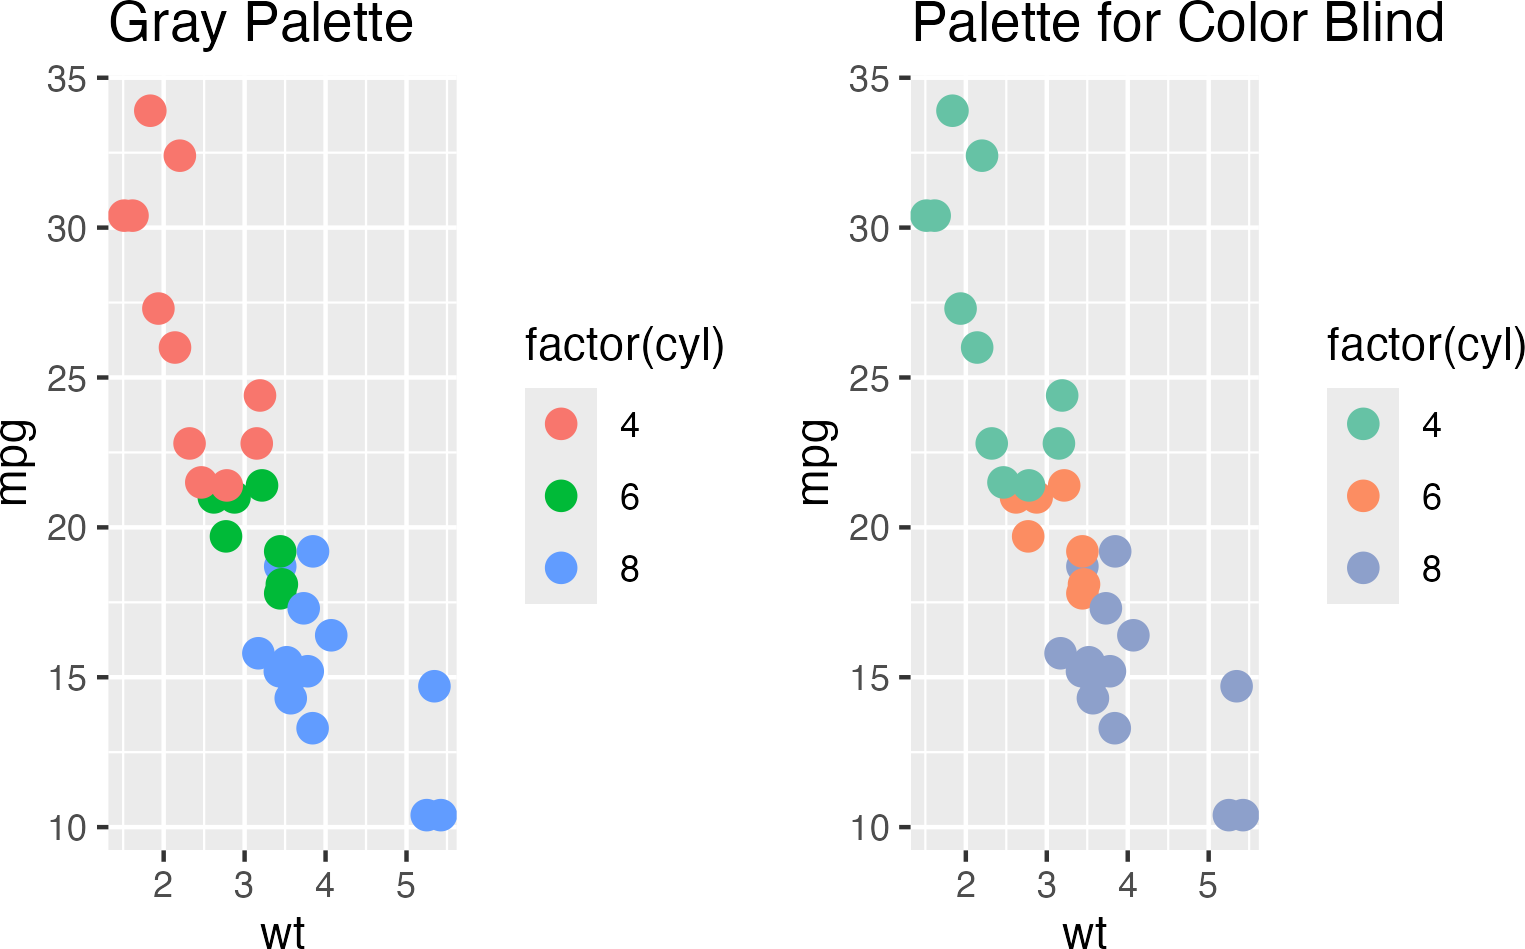
\includegraphics[keepaspectratio]{chapter04_files/figure-pdf/unnamed-chunk-2-1.png}}

また,\texttt{ggplot2}のデフォルト設定では,背景色が灰色になっている。これは全体のテーマとして\texttt{theme\_gray()}が設定されているからである。しかし日本心理学会の\href{https://psych.or.jp/manual/}{執筆・投稿の手引き}に記載されているグラフの例を見ると,背景は白色とされている。このような設定に変更するためには,theme\_classic()やtheme\_bw()を用いる。

\begin{Shaded}
\begin{Highlighting}[]
\NormalTok{p2 }\SpecialCharTok{+} \FunctionTok{theme\_classic}\NormalTok{()}
\end{Highlighting}
\end{Shaded}

\pandocbounded{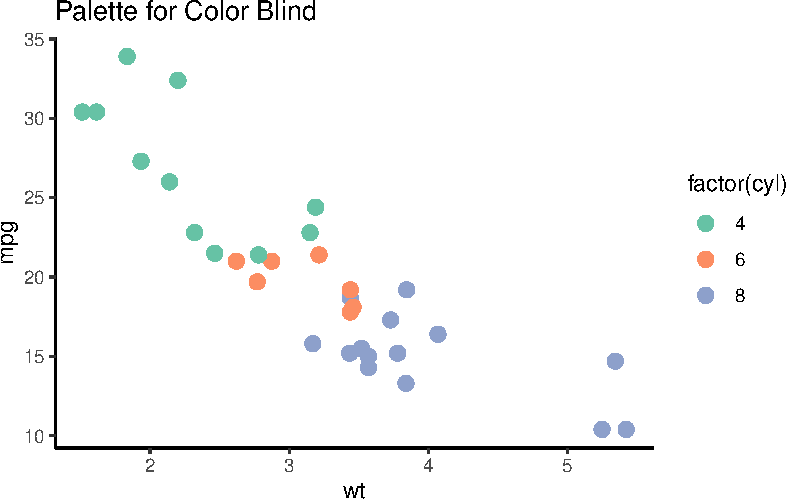
\includegraphics[keepaspectratio]{chapter04_files/figure-pdf/unnamed-chunk-3-1.pdf}}

このほかにも,様々な描画上の工夫は考えられる。目標となる図版のレシピを書き起こせるように,要素に分解ができれば,殆どのケースにおいて問題を解決することができるだろう。

\section{課題}\label{ux8ab2ux984c-2}

\begin{itemize}
\tightlist
\item
  今日の課題はRmarkdownで記述してください。著者名に学籍番号と名前を含め、適宜見出しをつくり、平文で以下に挙げる課題を記載することでどの課題に対する回答のコード(チャンク)であるかわかるようにしてください。
\end{itemize}

\begin{enumerate}
\def\labelenumi{\arabic{enumi}.}
\tightlist
\item
  \texttt{Baseball.csv}を読み込み、2020年度のデータセットに限定し、以下の操作に必要であれば変数の変換を済ませたデータセット、\texttt{dat.tb}を用意してください。
\item
  \texttt{dat.tb}の身長変数を使って、ヒストグラムを描いてください。この時、テーマを\texttt{theme\_classic}にしてください。
\item
  \texttt{dat.tb}の身長変数と体重変数を使って、散布図を描いてください。この時、テーマを\texttt{theme\_bw}にしてください。
\item
  (承前)
  散布図の各点を血液型で塗り分けてください。この時、カラーパレットを\texttt{Set3}に変えてください。
\item
  (承前) 散布図の点の形を血液型で変えてください。
\item
  \texttt{dat.tb}の身長と体重についての散布図を、チームごとに分割してください。
\item
  (承前)
  \texttt{geom\_smooth()}でスムーズな線を引いてください。特に\texttt{method}を指定する必要はありません。
\item
  (承前)
  \texttt{geom\_smooth()}で直線関数を引いてください。\texttt{method="lm"}と指定するといいでしょう。
\item
  x軸は身長、y軸は体重の平均値をプロットしてください。方法はいろいろありますが、要約統計量を計算した別のデータセット\texttt{dat.tb2}を作るか、幾何学オブジェクトの中で、次のように関数を適用することもできます。ヒント:\texttt{geom\_point(stat="summary",\ fun=mean)}。
\item
  課題2,
  4および体重のヒストグラムを使って下の図を描き、\texttt{ggsave}関数を使って保存するコードを書いてください。ファイル名やその他オプションは任意です。
\end{enumerate}

\pandocbounded{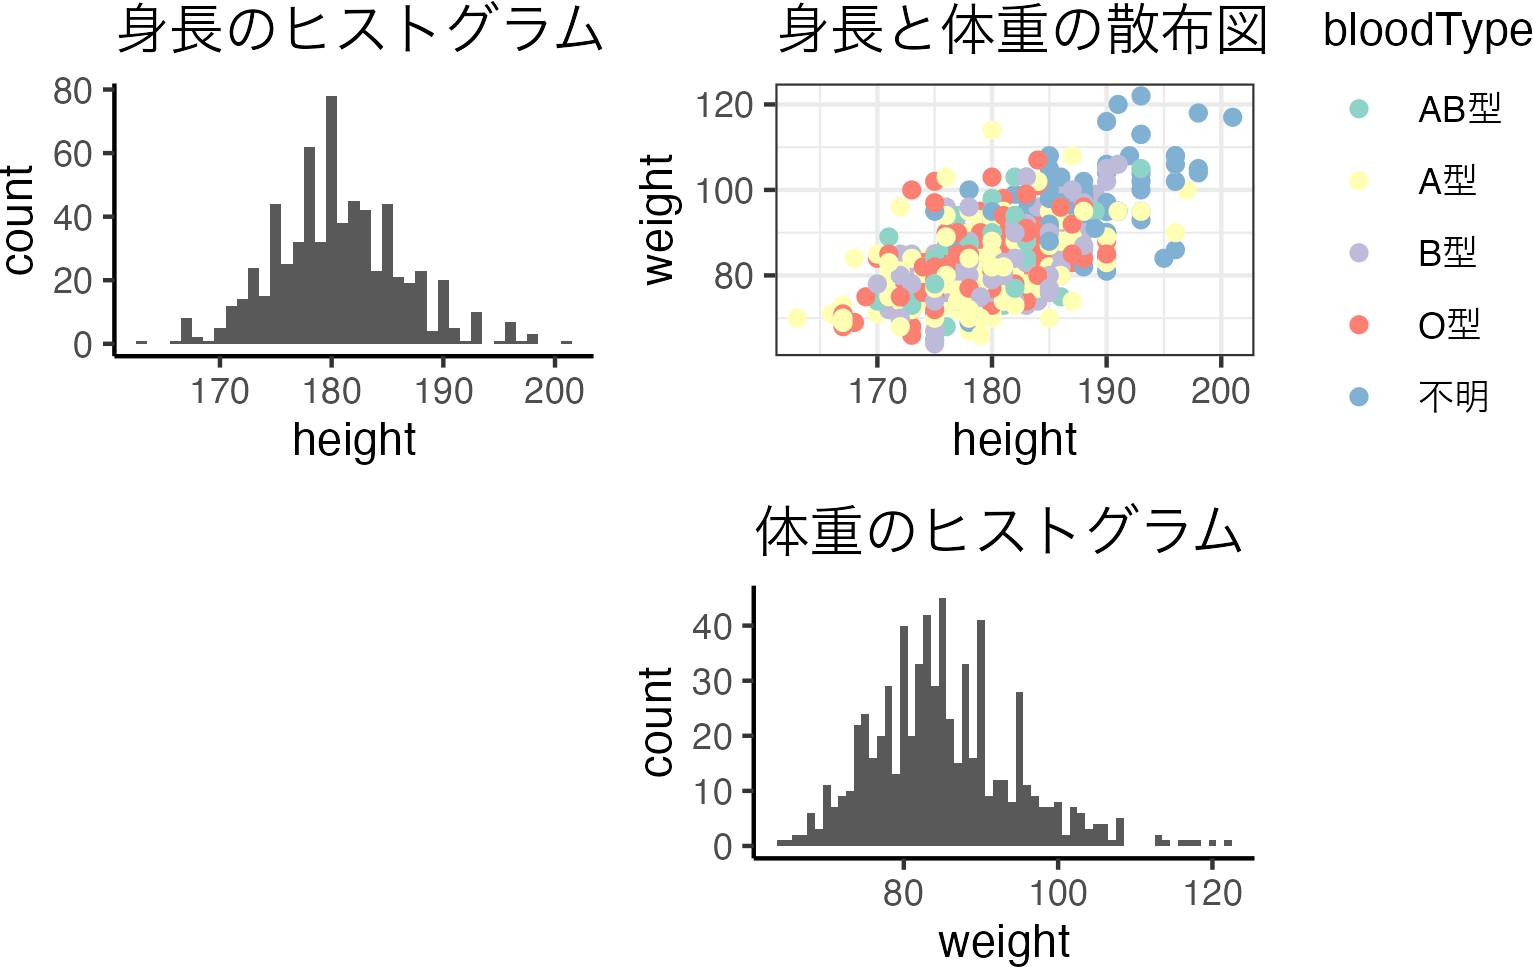
\includegraphics[keepaspectratio]{chapter04_files/figure-pdf/unnamed-chunk-4-1.png}}

\bookmarksetup{startatroot}

\chapter{Rでプログラミング}\label{rux3067ux30d7ux30edux30b0ux30e9ux30dfux30f3ux30b0}

ここではプログラミング言語としてのRについて解説する。 なお副読本として
\textcite{kosugi2023}
を挙げておく。また,プログラミングのより専門的な理解のために,\textcite{Jared_P_Lander2018-12-28},
\textcite{Ren_Kun2017-11-23}, \textcite{Hadley_Wickham2016-02-10}
なども参考にすると良い。

プログラミング言語は,古くはCやJava,最近ではPythonやJuliaなどがよく用いられている。Rも統計パッケージというよりプログラミング言語として考えるのが適切かもしれない。Rは他のプログラミング言語に比べて,変数の型宣言を事前にしなくても良いことや,インデントなど書式についておおらかなところは,初心者にとって使いやすいところだろう。一方で,ベクトルの再利用のところで注意したように(Section~\ref{sec-vector}),不足分を補うために先回りして補填されたり,この後解説する関数の作成時に明示的な指定がなければ環境変数を参照する点など,親切心が空回りするところがある。より厳格な他言語になれていると,こうした点はかえって不便に思えるところもあるかもしれない。総じて,R言語は初心者向けであるといえるだろう。

さて,世にプログラミング言語は多くあれど\footnote{\textcite{Language2016}
  には117種もの計算機言語が紹介されている。},その全てに精通する必要はないし,不可能である。それよりも,プログラミング言語一般に通底する基本的概念を知り,あとは各言語による「方言」がある,と考えた方が生産的である。その基本的概念を3つ挙げるとすれば,「代入」「反復」「条件分岐」になるだろう。

\section{代入}\label{ux4ee3ux5165}

代入は,言い換えればオブジェクト(メモリ)に保管することを指す。これについては既に
Chapter~\ref{sec-Rbase}
で触れた通りであり,ここでは言及しない。オブジェクトや変数の型,常に上書きされる性質に注意しておけば十分だろう。

一点だけ追加で説明しておくと,次のような表現がなされることがある。

\begin{Shaded}
\begin{Highlighting}[]
\NormalTok{a }\OtherTok{\textless{}{-}} \DecValTok{0}
\NormalTok{a }\OtherTok{\textless{}{-}}\NormalTok{ a }\SpecialCharTok{+} \DecValTok{1}
\FunctionTok{print}\NormalTok{(a)}
\end{Highlighting}
\end{Shaded}

\begin{verbatim}
[1] 1
\end{verbatim}

ここではあえて,代入記号として\texttt{=}を使った。2行目に\texttt{a\ =\ a\ +\ 1}
とあるが,これを見て数式のように解釈しようとすると混乱する。数学的には明らかにおかしな表現だが,これは上書きと代入というプログラミング言語の特徴を使ったもので,「(いま保持している)\texttt{a}の値に1を加えたものを,(新しく同じ名前のオブジェクト)\texttt{a}に代入する(=上書きする)」という意味である。この方法で,\texttt{a}
をカウンタ変数として用いることがある。誤読の可能性を下げるため,この授業においては代入記号を\texttt{\textless{}-}としている。

このオブジェクトを上書きするという特徴は多くの言語に共通したものであり,間違いを避けるためには,オブジェクトを作る時に初期値を設定することが望ましい。先の例では,代入の直上で\texttt{a\ \textless{}-\ 0}としており,オブジェクト\texttt{a}
に\texttt{0}
を初期値として与えている。この変数の初期化作業がないと,以前に使っていた値を引き継いでしまう可能性があるので,今から新しく使う変数を作りたいというときは,このように明示しておくといいだろう。

なお,変数をメモリから明示的に削除する場合は,\texttt{remove}関数を使う。

\begin{Shaded}
\begin{Highlighting}[]
\FunctionTok{remove}\NormalTok{(a)}
\end{Highlighting}
\end{Shaded}

これを実行すると,RStudioのEnvironmentタブからオブジェクト\texttt{a}が消えたことがわかるだろう。
メモリの一斉除去は,同じくRStudioのEnvironmentタブにある箒マークをクリックするか,\texttt{remove(list=ls())}とすると良い\footnote{\texttt{ls()}関数はlist
  objectsの意味で,メモリにあるオブジェクトのリストを作る関数}。

\section{反復}\label{ux53cdux5fa9}

\subsection{for文}\label{forux6587}

電子計算機の特徴は,電源等のハードウェア的問題がなければ疲労することなく計算を続けられるところにある。人間は反復によって疲労が溜まったり,集中力が欠如するなどして単純ミスを生成するが,電子計算機にそういったところはない。

このように反復計算は電子計算機の中心的特徴であり,細々した計算作業を指示した期間反復させ続けることができる。反復の代表的なコマンドは\texttt{for}であり,forループなどと呼ばれる。forループはプログラミングの基本的な制御構造であり,R言語の\texttt{for}ループの基本的な構文は次のようになる:

\begin{Shaded}
\begin{Highlighting}[]
\ControlFlowTok{for}\NormalTok{ (value }\ControlFlowTok{in}\NormalTok{ sequence) \{}
    \CommentTok{\# 実行するコード}
\NormalTok{\}}
\end{Highlighting}
\end{Shaded}

ここの\texttt{value}は各反復で\texttt{sequence}の次の要素を取る反復インデックス変数である。。\texttt{sequence}は一般にベクトルやリストなどの配列型のデータであり,「\#実行するコード」はループ体内で実行される一連の命令になる。

以下は\texttt{for}文の例である。

\begin{Shaded}
\begin{Highlighting}[]
\ControlFlowTok{for}\NormalTok{ (i }\ControlFlowTok{in} \DecValTok{1}\SpecialCharTok{:}\DecValTok{5}\NormalTok{) \{}
  \FunctionTok{cat}\NormalTok{(}\StringTok{"現在の値は"}\NormalTok{, i, }\StringTok{"です。}\SpecialCharTok{\textbackslash{}n}\StringTok{"}\NormalTok{)}
\NormalTok{\}}
\end{Highlighting}
\end{Shaded}

\begin{verbatim}
現在の値は 1 です。
現在の値は 2 です。
現在の値は 3 です。
現在の値は 4 です。
現在の値は 5 です。
\end{verbatim}

\texttt{for}
文は続く小括弧のなかである変数を宣言し(ここでは\texttt{i}),それがどのように変化するか(ここでは\texttt{1:5},すなわち1,2,3,4,5)を指定する。続く中括弧の中で,反復したい操作を記入する。今回は\texttt{cat}
文によるコンソールへの文字力の出力を行っている。ここでのコマンドは複数あってもよく,中括弧が閉じられるまで各行のコマンドが実行される。

次に示すは,\texttt{sequence}にあるベクトルが指定されているので,反復インデックス変数が連続的に変化しない例である。

\begin{Shaded}
\begin{Highlighting}[]
\ControlFlowTok{for}\NormalTok{ (i }\ControlFlowTok{in} \FunctionTok{c}\NormalTok{(}\DecValTok{2}\NormalTok{, }\DecValTok{4}\NormalTok{, }\DecValTok{12}\NormalTok{, }\DecValTok{3}\NormalTok{, }\SpecialCharTok{{-}}\DecValTok{6}\NormalTok{)) \{}
  \FunctionTok{cat}\NormalTok{(}\StringTok{"現在の値は"}\NormalTok{, i, }\StringTok{"です。}\SpecialCharTok{\textbackslash{}n}\StringTok{"}\NormalTok{)}
\NormalTok{\}}
\end{Highlighting}
\end{Shaded}

\begin{verbatim}
現在の値は 2 です。
現在の値は 4 です。
現在の値は 12 です。
現在の値は 3 です。
現在の値は -6 です。
\end{verbatim}

また,反復はネスト(入れ子)になることもできる。次の例を見てみよう。

\begin{Shaded}
\begin{Highlighting}[]
\CommentTok{\# 2次元の行列を定義}
\NormalTok{A }\OtherTok{\textless{}{-}} \FunctionTok{matrix}\NormalTok{(}\DecValTok{1}\SpecialCharTok{:}\DecValTok{9}\NormalTok{, }\AttributeTok{nrow =} \DecValTok{3}\NormalTok{)}

\CommentTok{\# 行ごとにループ}
\ControlFlowTok{for}\NormalTok{ (i }\ControlFlowTok{in} \DecValTok{1}\SpecialCharTok{:}\FunctionTok{nrow}\NormalTok{(A)) \{}
  \CommentTok{\# 列ごとにループ}
  \ControlFlowTok{for}\NormalTok{ (j }\ControlFlowTok{in} \DecValTok{1}\SpecialCharTok{:}\FunctionTok{ncol}\NormalTok{(A)) \{}
    \FunctionTok{cat}\NormalTok{(}\StringTok{"要素 ["}\NormalTok{, i, }\StringTok{", "}\NormalTok{, j, }\StringTok{"]は "}\NormalTok{, A[i, j], }\StringTok{"}\SpecialCharTok{\textbackslash{}n}\StringTok{"}\NormalTok{)}
\NormalTok{  \}}
\NormalTok{\}}
\end{Highlighting}
\end{Shaded}

\begin{verbatim}
要素 [ 1 ,  1 ]は  1 
要素 [ 1 ,  2 ]は  4 
要素 [ 1 ,  3 ]は  7 
要素 [ 2 ,  1 ]は  2 
要素 [ 2 ,  2 ]は  5 
要素 [ 2 ,  3 ]は  8 
要素 [ 3 ,  1 ]は  3 
要素 [ 3 ,  2 ]は  6 
要素 [ 3 ,  3 ]は  9 
\end{verbatim}

ここで,反復インデックス変数が\texttt{i}と\texttt{j}というように異なる名称になっていることに注意しよう。例えば今回,ここで両者を\texttt{i}にしてしまうと,行変数なのか列変数なのかわからなくなってしまう。また少し専門的になるが,R言語は\texttt{for}文で宣言されるたびに,内部で反復インデックス変数を新しく生成している(異なるメモリを割り当てる)ためにエラーにならないが,他言語の場合は同じ名前のオブジェクトと判断されることが一般的であり,その際は値が終了値に到達せず計算が終わらないといったバグを引き起こす。反復に使う汎用的な変数名として\texttt{i,j,k}がよく用いられるため,自身のスクリプトの中でオブジェクト名として単純な一文字にすることは避けた方がいいだろう。

\subsection{while文}\label{whileux6587}

whileループはプログラミングの基本構造であり,特定の条件が真(True)である間,繰り返し一連の命令を実行する。「``while''(~する間)」という名前から直感的に理解できるだろう。

R言語のwhileループの基本的な構文は次のようになる:

\begin{Shaded}
\begin{Highlighting}[]
\ControlFlowTok{while}\NormalTok{ (condition) \{}
    \CommentTok{\# 実行するコード}
\NormalTok{\}}
\end{Highlighting}
\end{Shaded}

ここで,「condition」はループが終了するための条件である。「\#
実行するコード」はループ体内で実行される一連の指示である。たとえば,1から10までの値を出力する\texttt{while}ループは以下のように書くことができる:

\begin{Shaded}
\begin{Highlighting}[]
\NormalTok{i }\OtherTok{\textless{}{-}} \DecValTok{1}
\ControlFlowTok{while}\NormalTok{ (i }\SpecialCharTok{\textless{}=} \DecValTok{5}\NormalTok{) \{}
  \FunctionTok{print}\NormalTok{(i)}
\NormalTok{  i }\OtherTok{\textless{}{-}}\NormalTok{ i }\SpecialCharTok{+} \DecValTok{1}
\NormalTok{\}}
\end{Highlighting}
\end{Shaded}

\begin{verbatim}
[1] 1
[1] 2
[1] 3
[1] 4
[1] 5
\end{verbatim}

このコードでは,「i」が5以下である限りループが続く。「print(i)」で「i」の値が表示され,「i
\textless- i +
1」で「i」の値が1ずつ増加する。これにより,「i」の値が5を超えると条件が偽(False)となり,ループが終了する。

whileループを使用する際の一般的な注意点は,無限ループ(終わらないループ)を避けることである。これは,conditionが常に真(True)である場合に発生する。そのような状況を避けるためには,ループ内部で何らかの形でconditionが最終的に偽(False)となるようにコードを記述することが必要である。

また,R言語は他の多くのプログラミング言語と異なり,ベクトル化された計算を効率的に行う設計がされている。したがって,可能な限り\texttt{for}ループや\texttt{while}ループを使わずに,ベクトル化した表現を利用すれば計算速度を上げることができる。

\section{条件分岐}\label{ux6761ux4ef6ux5206ux5c90}

条件分岐はプログラム内で特定の条件を指定し,その条件が満たされるかどうかによって異なる処理を行うための制御構造である。R言語では
\texttt{if-else} を用いて条件分岐を表現する。

\subsection{\texorpdfstring{\texttt{if}
文の基本的な構文}{if 文の基本的な構文}}\label{if-ux6587ux306eux57faux672cux7684ux306aux69cbux6587}

以下が \texttt{if} 文の基本的な構文になる:

\begin{Shaded}
\begin{Highlighting}[]
\ControlFlowTok{if}\NormalTok{ (条件) \{}
    \CommentTok{\# 条件が真である場合に実行するコード}
\NormalTok{\}}
\end{Highlighting}
\end{Shaded}

\texttt{if}
の後の小括弧内に条件を指定する。この条件が真(TRU)であれば,その後の
中括弧\texttt{\{\}} 内のコードが実行される。さらに,\texttt{else}
を使用して,条件が偽(FALSE)の場合の処理を追加することもできる:

\begin{Shaded}
\begin{Highlighting}[]
\ControlFlowTok{if}\NormalTok{ (条件) \{}
    \CommentTok{\# 条件が真である場合に実行するコード}
\NormalTok{\} }\ControlFlowTok{else}\NormalTok{ \{}
    \CommentTok{\# 条件が偽である場合に実行するコード}
\NormalTok{\}}
\end{Highlighting}
\end{Shaded}

以下に具体的な使用例を示そう:

\begin{Shaded}
\begin{Highlighting}[]
\NormalTok{x }\OtherTok{\textless{}{-}} \DecValTok{10}

\ControlFlowTok{if}\NormalTok{ (x }\SpecialCharTok{\textgreater{}} \DecValTok{0}\NormalTok{) \{}
  \FunctionTok{print}\NormalTok{(}\StringTok{"x is positive"}\NormalTok{)}
\NormalTok{\} }\ControlFlowTok{else}\NormalTok{ \{}
  \FunctionTok{print}\NormalTok{(}\StringTok{"x is not positive"}\NormalTok{)}
\NormalTok{\}}
\end{Highlighting}
\end{Shaded}

\begin{verbatim}
[1] "x is positive"
\end{verbatim}

このコードでは,変数 \texttt{x}
が正の場合とそうでない場合で異なるメッセージを出力する。

条件は論理式(例:\texttt{x\ \textgreater{}\ 0},
\texttt{y\ ==\ 1})や論理値(TRUE/FALSE)を返す関数・操作(例:\texttt{is.numeric(x)})などで指定する。また,複数の条件を組み合わせる際には論理演算子(\texttt{\&\&},
\texttt{\textbar{}\textbar{}})を使用する。

この例では,\texttt{x}が正と\texttt{y}が負の場合に特定のメッセージを出力する。それ以外の場合は,「Other
case」と出力される。\texttt{x}や\texttt{y}の値を色々変えて,試してみて欲しい。

\begin{Shaded}
\begin{Highlighting}[]
\NormalTok{x }\OtherTok{\textless{}{-}} \DecValTok{10}
\NormalTok{y }\OtherTok{\textless{}{-}} \SpecialCharTok{{-}}\DecValTok{3}

\ControlFlowTok{if}\NormalTok{ (x }\SpecialCharTok{\textgreater{}} \DecValTok{0} \SpecialCharTok{\&\&}\NormalTok{ y }\SpecialCharTok{\textless{}} \DecValTok{0}\NormalTok{) \{}
  \FunctionTok{print}\NormalTok{(}\StringTok{"x is positive and y is negative"}\NormalTok{)}
\NormalTok{\} }\ControlFlowTok{else}\NormalTok{ \{}
  \FunctionTok{print}\NormalTok{(}\StringTok{"Other case"}\NormalTok{)}
\NormalTok{\}}
\end{Highlighting}
\end{Shaded}

\begin{verbatim}
[1] "x is positive and y is negative"
\end{verbatim}

\section{反復と条件分岐に関する練習問題}\label{ux53cdux5fa9ux3068ux6761ux4ef6ux5206ux5c90ux306bux95a2ux3059ux308bux7df4ux7fd2ux554fux984c}

\begin{enumerate}
\def\labelenumi{\arabic{enumi}.}
\tightlist
\item
  1から20までの数字で,偶数だけをプリントするプログラムを書いてください。
\item
  1から40までの数値をプリントするプログラムを書いてください。ただしその数値に3がつく(1か10の位の値が3である)か,3の倍数の時だけ,数字の後ろに「サァン!」という文字列をつけて出力してください。
\item
  ベクトル \texttt{c(1,\ -2,\ 3,\ -4,\ 5)} の各要素について,正なら
  ``positive'',負なら ``negative''
  をプリントするプログラムを書いてください。
\item
  次の行列\(A\)と\(B\)の掛け算を計算するプログラムを書いてください。なお,Rで行列の積は\texttt{\%*\%}という演算子を使いますが,ここでは\texttt{for}文を使ったプログラムにしてください。出来上がる行列の\(i\)行\(j\)列目の要素\(c_{ij}\)は,行列\(A\)の第\(i\)行の各要素と,行列\(B\)の第\(j\)列目の各要素の積和,すなわち\[c_{ij}=\sum_{k} a_{ik}b_{kj}\]になります。検算用のコードを下に示します。
\end{enumerate}

\begin{Shaded}
\begin{Highlighting}[]
\NormalTok{A }\OtherTok{\textless{}{-}} \FunctionTok{matrix}\NormalTok{(}\DecValTok{1}\SpecialCharTok{:}\DecValTok{6}\NormalTok{, }\AttributeTok{nrow =} \DecValTok{3}\NormalTok{)}
\NormalTok{B }\OtherTok{\textless{}{-}} \FunctionTok{matrix}\NormalTok{(}\DecValTok{3}\SpecialCharTok{:}\DecValTok{10}\NormalTok{, }\AttributeTok{nrow =} \DecValTok{2}\NormalTok{)}
\DocumentationTok{\#\# 課題になる行列}
\FunctionTok{print}\NormalTok{(A)}
\end{Highlighting}
\end{Shaded}

\begin{verbatim}
     [,1] [,2]
[1,]    1    4
[2,]    2    5
[3,]    3    6
\end{verbatim}

\begin{Shaded}
\begin{Highlighting}[]
\FunctionTok{print}\NormalTok{(B)}
\end{Highlighting}
\end{Shaded}

\begin{verbatim}
     [,1] [,2] [,3] [,4]
[1,]    3    5    7    9
[2,]    4    6    8   10
\end{verbatim}

\begin{Shaded}
\begin{Highlighting}[]
\DocumentationTok{\#\# 求めるべき答え}
\NormalTok{C }\OtherTok{\textless{}{-}}\NormalTok{ A }\SpecialCharTok{\%*\%}\NormalTok{ B}
\FunctionTok{print}\NormalTok{(C)}
\end{Highlighting}
\end{Shaded}

\begin{verbatim}
     [,1] [,2] [,3] [,4]
[1,]   19   29   39   49
[2,]   26   40   54   68
[3,]   33   51   69   87
\end{verbatim}

\section{関数を作る}\label{ux95a2ux6570ux3092ux4f5cux308b}

複雑なプログラムも,ここまでの代入、反復,条件分岐の組み合わせからなる。回帰分析や因子分析のような統計モデルを実行するときに,統計パッケージのユーザとしては,統計モデルを実現してくれる関数にデータを与えて答えを受け取るだけであるが,そのアルゴリズムはこれらプログラミングのピースを紡いでつくられているのである。

ここでは関数を自分で作ることを考える。といっても身構える必要はない。表計算ソフトウェアで同じような操作を繰り返すときにマクロに記録するように,R上で同じようなコードを何度も書く機会があるならば,それを関数という名のパッケージにしておこう,ということである。関数化しておくことで手続きをまとめることができ,小単位に分割できるため並列して開発したり,バグを見つけやすくなるという利点がある。

\subsection{基本的な関数の作り方}\label{ux57faux672cux7684ux306aux95a2ux6570ux306eux4f5cux308aux65b9}

関数が受け取る値のことを\textbf{引数}(ひきすう,argument)といい,また関数が返す値のことを\textbf{戻り値}(もどりち,value)という。\(y=f(x)\)という式は,引数が\texttt{x}で戻り値が\texttt{y}な関数\(f\),と言い換えることができるだろう。

Rの関数を書く基本的な構文は以下のようになる。

\begin{Shaded}
\begin{Highlighting}[]
\NormalTok{function\_name }\OtherTok{\textless{}{-}} \ControlFlowTok{function}\NormalTok{(argument) \{}
   \CommentTok{\# function body}
   \FunctionTok{return}\NormalTok{(value)}
\NormalTok{\}}
\end{Highlighting}
\end{Shaded}

ここで\texttt{function\ body}とあるのは計算本体である。例えば与えられた数字に\texttt{3}を足して返す関数,\texttt{add3}を作ってみよう。プログラムは以下のようになる。

\begin{Shaded}
\begin{Highlighting}[]
\NormalTok{add3 }\OtherTok{\textless{}{-}} \ControlFlowTok{function}\NormalTok{(x) \{}
\NormalTok{  x }\OtherTok{\textless{}{-}}\NormalTok{ x }\SpecialCharTok{+} \DecValTok{3}
  \FunctionTok{return}\NormalTok{(x)}
\NormalTok{\}}
\CommentTok{\# 実行例}
\FunctionTok{add3}\NormalTok{(}\DecValTok{5}\NormalTok{)}
\end{Highlighting}
\end{Shaded}

\begin{verbatim}
[1] 8
\end{verbatim}

また,2つの値を足し合わせる関数は次のようになる。

\begin{Shaded}
\begin{Highlighting}[]
\NormalTok{add\_numbers }\OtherTok{\textless{}{-}} \ControlFlowTok{function}\NormalTok{(a, b) \{}
\NormalTok{  sum }\OtherTok{\textless{}{-}}\NormalTok{ a }\SpecialCharTok{+}\NormalTok{ b}
  \FunctionTok{return}\NormalTok{(sum)}
\NormalTok{\}}
\CommentTok{\# 実行例}
\FunctionTok{add\_numbers}\NormalTok{(}\DecValTok{2}\NormalTok{, }\DecValTok{5}\NormalTok{)}
\end{Highlighting}
\end{Shaded}

\begin{verbatim}
[1] 7
\end{verbatim}

ここで示したように,引数は複数取ることも可能である。また,既定値default
valueを設定することも可能である。次の例を見てみよう。

\begin{Shaded}
\begin{Highlighting}[]
\NormalTok{add\_numbers2 }\OtherTok{\textless{}{-}} \ControlFlowTok{function}\NormalTok{(a, }\AttributeTok{b =} \DecValTok{1}\NormalTok{) \{}
\NormalTok{  sum }\OtherTok{\textless{}{-}}\NormalTok{ a }\SpecialCharTok{+}\NormalTok{ b}
  \FunctionTok{return}\NormalTok{(sum)}
\NormalTok{\}}
\CommentTok{\# 実行例}
\FunctionTok{add\_numbers2}\NormalTok{(}\DecValTok{2}\NormalTok{, }\DecValTok{5}\NormalTok{)}
\end{Highlighting}
\end{Shaded}

\begin{verbatim}
[1] 7
\end{verbatim}

\begin{Shaded}
\begin{Highlighting}[]
\FunctionTok{add\_numbers2}\NormalTok{(}\DecValTok{4}\NormalTok{)}
\end{Highlighting}
\end{Shaded}

\begin{verbatim}
[1] 5
\end{verbatim}

関数を作るときに,\texttt{(a,b=1)}としているのは,\texttt{b}に既定値として\texttt{1}を与えていて,特に指定がなければこの値を使うよう指示しているということである。実行例において,引数が2つ与えられている場合はそれらを使った計算をし(\texttt{2+5}),1つしか与えられていない場合は第一引数\texttt{a}に与えられた値を,第二引数\texttt{b}は既定値を使った計算をする(\texttt{4+1}),という挙動になる。

ここから推察できるように,われわれユーザが使う統計パッケージの関数にも実は多くの引数があり,既定値が与えられているということだ。これらは選択的に,あるいは能動的に与えることができるものであるが,これらの引数は選択的に指定することができるのだが,通常は一般的に使われる値や計算の細かな設定に関するものであり,開発者がユーザの手間を省くために提供しているものである。関数のヘルプを見ると指定可能な引数の一覧が表示されるので,ぜひ興味を持って見てもらいたい。

\subsection{複数の戻り値}\label{ux8907ux6570ux306eux623bux308aux5024}

Rでの戻り値は1つのオブジェクトでなければならない。しかし,複数の値を返したいということがあるだろう。そのような場合は,返すオブジェクトを\texttt{list}などでひとまとめにして作成すると良い。以下に簡単な例を示す。

\begin{Shaded}
\begin{Highlighting}[]
\NormalTok{calculate\_values }\OtherTok{\textless{}{-}} \ControlFlowTok{function}\NormalTok{(a, b) \{}
\NormalTok{  sum }\OtherTok{\textless{}{-}}\NormalTok{ a }\SpecialCharTok{+}\NormalTok{ b}
\NormalTok{  diff }\OtherTok{\textless{}{-}}\NormalTok{ a }\SpecialCharTok{{-}}\NormalTok{ b}
  \CommentTok{\# 戻り値として名前付きリストを作成}
\NormalTok{  result }\OtherTok{\textless{}{-}} \FunctionTok{list}\NormalTok{(}\StringTok{"sum"} \OtherTok{=}\NormalTok{ sum, }\StringTok{"diff"} \OtherTok{=}\NormalTok{ diff)}
  \FunctionTok{return}\NormalTok{(result)}
\NormalTok{\}}
\CommentTok{\# 実行例}
\NormalTok{result }\OtherTok{\textless{}{-}} \FunctionTok{calculate\_values}\NormalTok{(}\DecValTok{10}\NormalTok{, }\DecValTok{5}\NormalTok{)}
\CommentTok{\# 結果を表示}
\FunctionTok{print}\NormalTok{(result)}
\end{Highlighting}
\end{Shaded}

\begin{verbatim}
$sum
[1] 15

$diff
[1] 5
\end{verbatim}

\section{課題}\label{ux8ab2ux984c-3}

\begin{enumerate}
\def\labelenumi{\arabic{enumi}.}
\tightlist
\item
  ある値を与えたとき,正の値なら''positive'',負の値なら''negative'',0のときは''Zero''と表示する関数を書いてください。
\item
  ある2組の数字を与えた時,和,差,積,商を返す関数を書いてください。
\item
  あるベクトルを与えた時,算術平均,中央値,最大値,最小値,範囲を返す関数を書いてください。
\item
  あるベクトルを与えた時,標本分散を返す関数を書いてください。なおRの分散を返す関数\texttt{var}は不偏分散\(\hat{\sigma}\)を返しており,標本分散\texttt{v}とは計算式が異なります。念のため,計算式を以下に示します。
  \[\hat{\sigma} = \frac{1}{n-1}\sum_{i=1}^n (x_i - \bar{x})^2 \]
  \[v= \frac{1}{n}\sum_{i=1}^n (x_i - \bar{x})^2 \]
\end{enumerate}

\bookmarksetup{startatroot}

\chapter{確率とシミュレーション}\label{ux78baux7387ux3068ux30b7ux30dfux30e5ux30ecux30fcux30b7ux30e7ux30f3}

\section{確率の考え方と使い所}\label{ux78baux7387ux306eux8003ux3048ux65b9ux3068ux4f7fux3044ux6240}

統計と確率は密接な関係がある。
まずデータをたくさん集めると,個々のケースでは見られない全体的な傾向が見られるようになり,それを表現するのに確率の考え方を使う,というのがひとつ。
次にデータがそれほどたくさんなくとも,大きな全体の中から一部を取り出した標本Sampleと考えられるとき,標本は全体の性質をどのように反映しているかを考えることになる。ここで全体の傾向から一部を取り出した偶然性を表現するときに確率の考え方を使うことになる。
最後に,理論的・原理的に挙動がわかっている機械のようなものでも,現実的・実践的には系統だったズレが生じたり,偶然としか考えられない誤差が紛れ込むことがある。前者は機械の調整で対応できるが,後者は偶然が従う確率を考える必要がある。

心理学は人間を対象に研究を行うが,あらゆる人間を一度に調べるわけにはいかないので,サンプルを取り出して調査したり実験したりする(第2のケース)。データサイエンスでは何万レコードというおおきなデータセットになるが,心理学の場合は数件から数十件しかないことも多い。また,心理学的傾向を理論立ててモデル化できたとしても,実際の行動には誤差が含まれている可能性が高い(第3のケース)。このことから,心理学で得られるデータは確率変数として考えられ,小標本から母集団の性質を推測する\textbf{推測統計}と共に利用される。

厳密に数学的な意味での\textbf{確率}は,集合,積分,測度といった緻密な概念の積み重ねから定義される\footnote{詳しくは
  \textcite{Yoshida2021-02-25} , \textcite{Kono1999-05-01},
  \textcite{Sato1994-02-25} などを参照のこと。}。ここではその詳細に分け入らず,単に「特定の結果が生じる可能性について,0から1の間の実数でその大小を表現したもの」とだけ理解しておいて欲しい。この定義からは,「全ての可能な組み合わせのうち当該事象の成立する割合」という解釈も成り立つし,「主観的に重みづけた真実味の強さに関する信念の度合い」という解釈も成り立つ。\footnote{前者の解釈は高校までの数学で学ぶ確率であり,頻度主義的確率と呼ばれることがある。一方後者の解釈は,降水確率X\%のように日常でも使うものであり,主観確率と呼ばれることがある。こうした解釈の違いを,主義主張の対立であって数学的ではない,と批判する向きもあるが,実際コルモゴロフの公理はどちらの立場でも成立するように整えられており,筆者個人的にはユーザが理解しやすく計算できればどちらでも良いと考えている。}
これまで学んできた確率は順列・組み合わせを全て書き出す退屈なもの,と思っていたかもしれないが,「十中八九まちがいないね(80-90\%ほど確からしいと考えている)」という数字も確率の一種として扱えるので,非常に身近で適用範囲の広い概念である。理解を進めるポイントの1つとして,確率を面積として考えると良いかもしれない。ありうる状況の全体の空間に対して,事象の成立する程度がどの程度の面積がどの程度の割合であるかを表現したのが確率という量である,と考えるのである(
\textcite{Hiraoka200910}
は書籍の中で一貫して面積で説明している。この説明だと,条件付き確率などの理解がしやすい。)。

ただし注意して区別しておいて欲しいのが,確率変数とその実現値の違いである。データセットやスプレッドシートに含まれる値は,あくまでも\textbf{確率変数の実現値}(実際に観測された値)というのであって,\textbf{確率変数}はその不確実な状態を有した変数そのものを指す言葉である。サイコロは確率変数だが,サイコロの出目は確率変数の実現値である。心理変数は確率変数だが,手に入れたデータはその実現値である。実現値を通じて変数の特徴を知り,全体を推測するという流れである。

目の前のデータを超えて,抽象的な実体で議論を進めることが難しく感じられるかもしれない。実は誰しもそうなのであって,確率の正確な理解は非常に難易度が高い。しかしRなど計算機言語に実装されている関数を通じて,より具体的に,操作しながら理解することで徐々に理解していこう。

\section{確率分布の関数}\label{ux78baux7387ux5206ux5e03ux306eux95a2ux6570}

確率変数の実現値は,\textbf{確率分布}に従う。確率分布とは,その実現値がどの程度生じやすいかを全て表した総覧であり,一般的に関数で表現される。実現値が連続的か離散的かによって名称が異なるが,連続的な確率分布関数は\textbf{確率密度関数(Probability
Density
Function)},離散的な確率分布関数は\textbf{確率質量関数(Probability Mass
Function)}という。

Rには最初から確率に関する関数がいくつか準備されている。最も有名な確率分布である\textbf{正規分布}について,次のような関数がある。

\begin{Shaded}
\begin{Highlighting}[]
\CommentTok{\# 標準のプロット関数,curve}
\FunctionTok{curve}\NormalTok{(}\FunctionTok{dnorm}\NormalTok{(x), }\AttributeTok{from =} \SpecialCharTok{{-}}\DecValTok{4}\NormalTok{, }\AttributeTok{to =} \DecValTok{4}\NormalTok{)}
\end{Highlighting}
\end{Shaded}

\pandocbounded{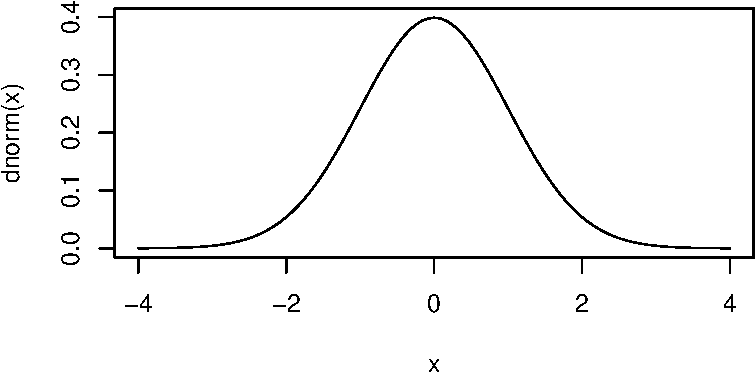
\includegraphics[keepaspectratio]{chapter06_files/figure-pdf/normal-1.pdf}}

\begin{Shaded}
\begin{Highlighting}[]
\CommentTok{\# ggplot2を使ってカッコよく}
\NormalTok{pacman}\SpecialCharTok{::}\FunctionTok{p\_load}\NormalTok{(tidyverse)}
\FunctionTok{data.frame}\NormalTok{(}\AttributeTok{x =} \FunctionTok{seq}\NormalTok{(}\SpecialCharTok{{-}}\DecValTok{4}\NormalTok{, }\DecValTok{4}\NormalTok{, }\AttributeTok{by =} \FloatTok{0.01}\NormalTok{)) }\SpecialCharTok{\%\textgreater{}\%}
  \FunctionTok{mutate}\NormalTok{(}\AttributeTok{y =} \FunctionTok{dnorm}\NormalTok{(x)) }\SpecialCharTok{\%\textgreater{}\%}
  \FunctionTok{ggplot}\NormalTok{(}\FunctionTok{aes}\NormalTok{(}\AttributeTok{x =}\NormalTok{ x, }\AttributeTok{y =}\NormalTok{ y)) }\SpecialCharTok{+}
  \FunctionTok{geom\_line}\NormalTok{() }\SpecialCharTok{+}
  \FunctionTok{theme\_classic}\NormalTok{()}
\end{Highlighting}
\end{Shaded}

\pandocbounded{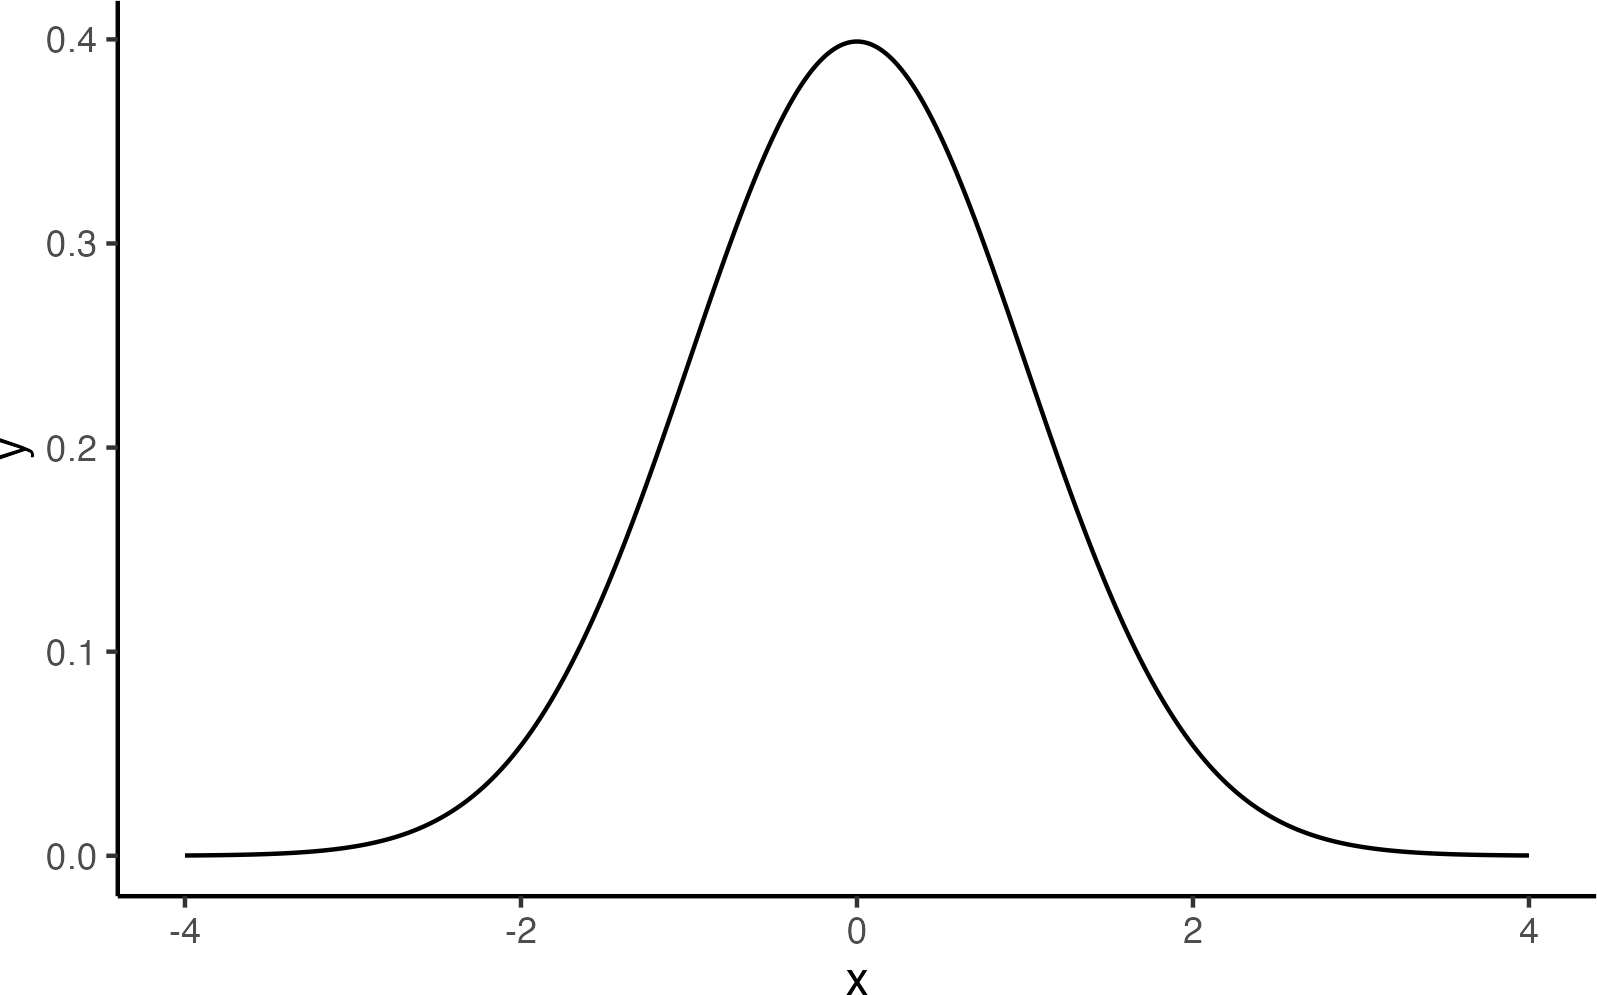
\includegraphics[keepaspectratio]{chapter06_files/figure-pdf/normlByggplot-1.png}}

ここで\texttt{dnorm}という関数を使っているが,\texttt{d}はDensity(確率密度)の頭文字であり,\texttt{norm}はNormal
Distribution(正規分布)の一部である。このように,Rでは確率分布の名前を表す名称(ここでは\texttt{norm})と,それに接頭文字ひとつ(\texttt{d})で関数を構成する。この接頭文字は他に\texttt{p},\texttt{q},\texttt{r}があり,\texttt{dpois}(ポアソン分布poisson
distributionの確率密度関数),\texttt{pnorm}(正規分布normal
distributionの累積分布関数),\texttt{rbinom}(二項分布binomial
distributionからの乱数生成)のように使う。

ここでは正規分布を例に説明を続けよう。正規分布は平均\(\mu\)と標準偏差\(\sigma\)でその形状が特徴づけられる。これらの確率分布の特徴を表す数字のことを\textbf{母数
parameter}という。たとえば,次の3つの曲線はパラメータが異なる正規分布である。

\begin{Shaded}
\begin{Highlighting}[]
\FunctionTok{data.frame}\NormalTok{(}\AttributeTok{x =} \FunctionTok{seq}\NormalTok{(}\SpecialCharTok{{-}}\DecValTok{4}\NormalTok{, }\DecValTok{4}\NormalTok{, }\AttributeTok{by =} \FloatTok{0.01}\NormalTok{)) }\SpecialCharTok{\%\textgreater{}\%}
  \FunctionTok{mutate}\NormalTok{(}
    \AttributeTok{y1 =} \FunctionTok{dnorm}\NormalTok{(x, }\AttributeTok{mean =} \DecValTok{0}\NormalTok{, }\AttributeTok{sd =} \DecValTok{1}\NormalTok{),}
    \AttributeTok{y2 =} \FunctionTok{dnorm}\NormalTok{(x, }\AttributeTok{mean =} \DecValTok{1}\NormalTok{, }\AttributeTok{sd =} \FloatTok{0.5}\NormalTok{),}
    \AttributeTok{y3 =} \FunctionTok{dnorm}\NormalTok{(x, }\AttributeTok{mean =} \SpecialCharTok{{-}}\DecValTok{1}\NormalTok{, }\AttributeTok{sd =} \DecValTok{2}\NormalTok{)}
\NormalTok{  ) }\SpecialCharTok{\%\textgreater{}\%}
  \FunctionTok{pivot\_longer}\NormalTok{(}\SpecialCharTok{{-}}\NormalTok{x) }\SpecialCharTok{\%\textgreater{}\%}
  \FunctionTok{ggplot}\NormalTok{(}\FunctionTok{aes}\NormalTok{(}\AttributeTok{x =}\NormalTok{ x, }\AttributeTok{y =}\NormalTok{ value, }\AttributeTok{color =}\NormalTok{ name)) }\SpecialCharTok{+}
  \FunctionTok{geom\_line}\NormalTok{()}
\end{Highlighting}
\end{Shaded}

\pandocbounded{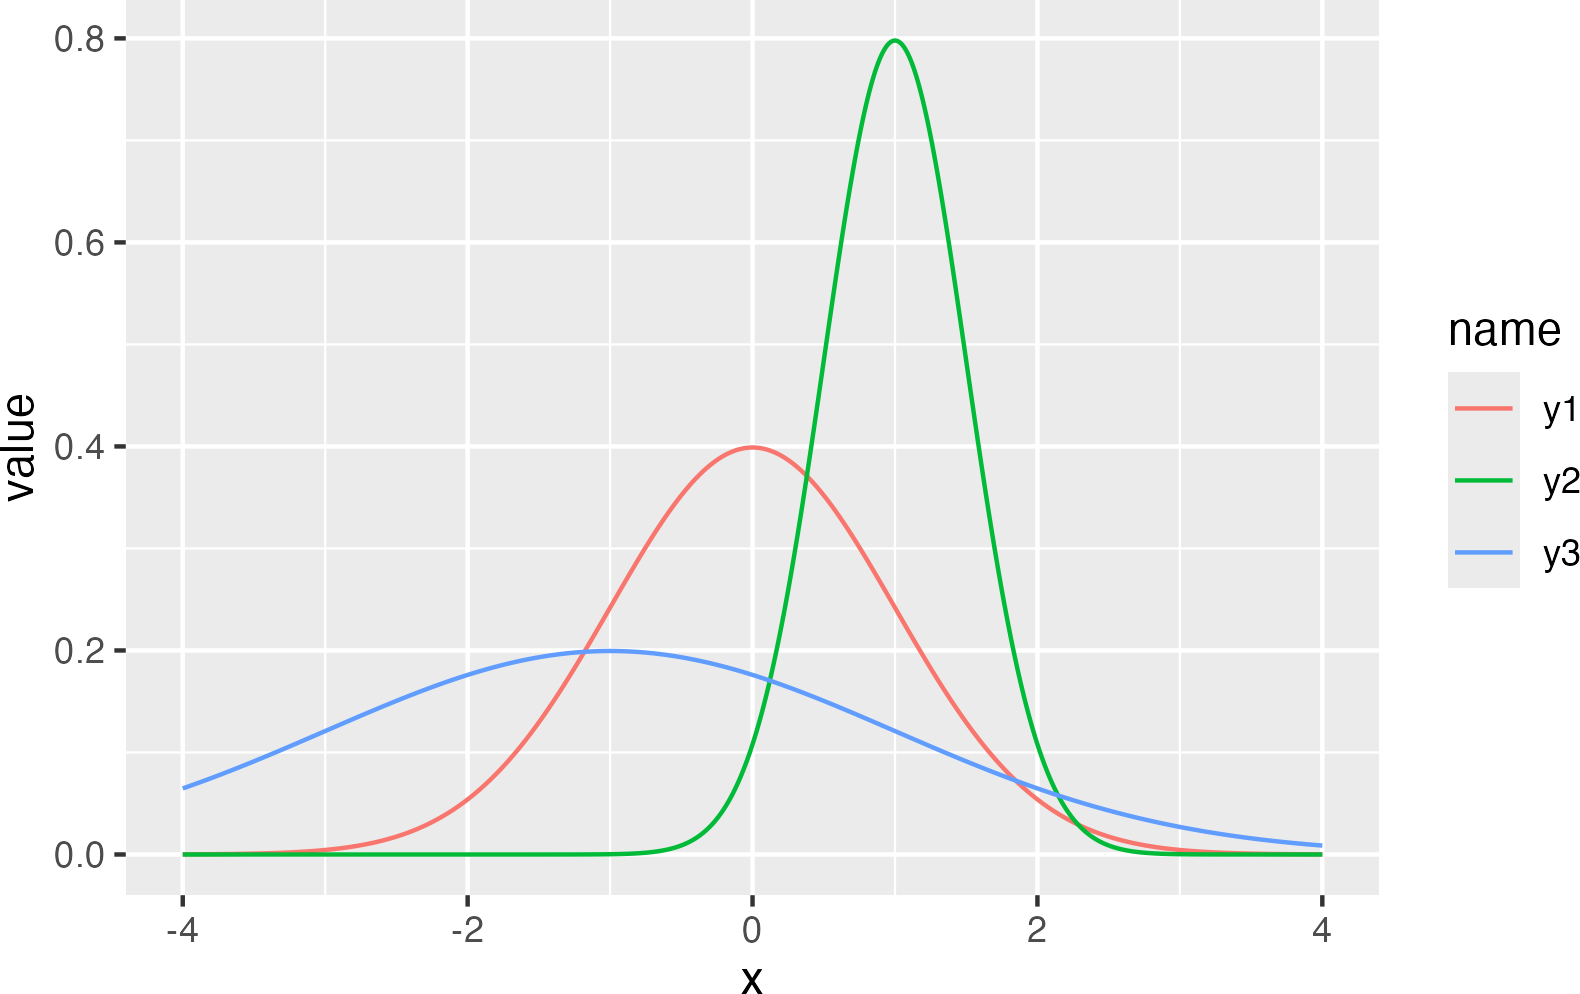
\includegraphics[keepaspectratio]{chapter06_files/figure-pdf/normals-1.png}}

平均は位置母数,標準偏差はスケール母数とも呼ばれ,分布の位置と幅を変えていることがわかる。言い換えると,データになるべく当てはまるように正規分布の母数を定めることもできるわけで,左右対称で単峰の分布という特徴があれば,正規分布でかなり様々なパターンを表せる。

さて,上の例で用いた関数はいずれも\texttt{d}を頭に持つ\texttt{dnorm}であり,確率分布の密度の高さを表現していた。では\texttt{p}や\texttt{q}が表すのは何であろうか。数値と図の例を示すので,その対応関係を確認してもらいたい。

\begin{Shaded}
\begin{Highlighting}[]
\CommentTok{\# 累積分布関数}
\FunctionTok{pnorm}\NormalTok{(}\FloatTok{1.96}\NormalTok{, }\AttributeTok{mean =} \DecValTok{0}\NormalTok{, }\AttributeTok{sd =} \DecValTok{1}\NormalTok{)}
\end{Highlighting}
\end{Shaded}

\begin{verbatim}
[1] 0.9750021
\end{verbatim}

\begin{Shaded}
\begin{Highlighting}[]
\CommentTok{\# 累積分布の逆関数}
\FunctionTok{qnorm}\NormalTok{(}\FloatTok{0.975}\NormalTok{, }\AttributeTok{mean =} \DecValTok{0}\NormalTok{, }\AttributeTok{sd =} \DecValTok{1}\NormalTok{)}
\end{Highlighting}
\end{Shaded}

\begin{verbatim}
[1] 1.959964
\end{verbatim}

数値で直感的にわかりにくい場合,次の図を見て確認しよう。\texttt{pnorm}関数はx座標の値を与えると,そこまでの面積(以下のコードで描かれる色付きの領域)すなわち確率を返す。\texttt{qnorm}関数は確率(=面積)を与えると,確率密度関数のカーブの下領域を積分してその値になるときのx座標の値を返す。

\begin{Shaded}
\begin{Highlighting}[]
\CommentTok{\# 描画}
\NormalTok{prob }\OtherTok{\textless{}{-}} \FloatTok{0.9}
\DocumentationTok{\#\# 全体の正規分布カーブ}
\NormalTok{df1 }\OtherTok{\textless{}{-}} \FunctionTok{data.frame}\NormalTok{(}\AttributeTok{x =} \FunctionTok{seq}\NormalTok{(}\AttributeTok{from =} \SpecialCharTok{{-}}\DecValTok{4}\NormalTok{, }\DecValTok{4}\NormalTok{, }\AttributeTok{by =} \FloatTok{0.01}\NormalTok{)) }\SpecialCharTok{\%\textgreater{}\%}
  \FunctionTok{mutate}\NormalTok{(}\AttributeTok{y =} \FunctionTok{dnorm}\NormalTok{(x, }\AttributeTok{mean =} \DecValTok{0}\NormalTok{, }\AttributeTok{sd =} \DecValTok{1}\NormalTok{))}
\DocumentationTok{\#\# qnorm(0.975)までのデータ}
\NormalTok{df2 }\OtherTok{\textless{}{-}} \FunctionTok{data.frame}\NormalTok{(}\AttributeTok{x =} \FunctionTok{seq}\NormalTok{(}\AttributeTok{from =} \SpecialCharTok{{-}}\DecValTok{4}\NormalTok{, }\FunctionTok{qnorm}\NormalTok{(prob), }\AttributeTok{by =} \FloatTok{0.01}\NormalTok{)) }\SpecialCharTok{\%\textgreater{}\%}
  \FunctionTok{mutate}\NormalTok{(}\AttributeTok{y =} \FunctionTok{dnorm}\NormalTok{(x, }\AttributeTok{mean =} \DecValTok{0}\NormalTok{, }\AttributeTok{sd =} \DecValTok{1}\NormalTok{))}
\DocumentationTok{\#\# データセットの違いに注意}
\FunctionTok{ggplot}\NormalTok{() }\SpecialCharTok{+}
  \FunctionTok{geom\_line}\NormalTok{(}\AttributeTok{data =}\NormalTok{ df1, }\FunctionTok{aes}\NormalTok{(}\AttributeTok{x =}\NormalTok{ x, }\AttributeTok{y =}\NormalTok{ y)) }\SpecialCharTok{+}
  \FunctionTok{geom\_ribbon}\NormalTok{(}\AttributeTok{data =}\NormalTok{ df2, }\FunctionTok{aes}\NormalTok{(}\AttributeTok{x =}\NormalTok{ x, }\AttributeTok{y =}\NormalTok{ y, }\AttributeTok{ymin =} \DecValTok{0}\NormalTok{, }\AttributeTok{ymax =}\NormalTok{ y), }\AttributeTok{fill =} \StringTok{"blue"}\NormalTok{, }\AttributeTok{alpha =} \FloatTok{0.3}\NormalTok{) }\SpecialCharTok{+}
  \DocumentationTok{\#\# 以下装飾}
  \FunctionTok{geom\_segment}\NormalTok{(}
    \FunctionTok{aes}\NormalTok{(}\AttributeTok{x =} \FunctionTok{qnorm}\NormalTok{(prob), }\AttributeTok{y =} \FunctionTok{dnorm}\NormalTok{(}\FunctionTok{qnorm}\NormalTok{(prob)), }\AttributeTok{xend =} \FunctionTok{qnorm}\NormalTok{(prob), }\AttributeTok{yend =} \DecValTok{0}\NormalTok{),}
    \AttributeTok{arrow =} \FunctionTok{arrow}\NormalTok{(}\AttributeTok{length =} \FunctionTok{unit}\NormalTok{(}\FloatTok{0.2}\NormalTok{, }\StringTok{"cm"}\NormalTok{)), }\AttributeTok{color =} \StringTok{"red"}
\NormalTok{  )}
\end{Highlighting}
\end{Shaded}

\pandocbounded{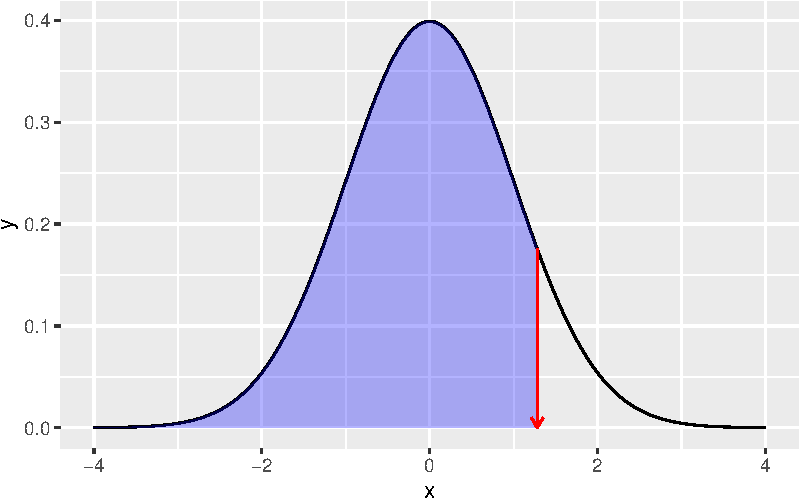
\includegraphics[keepaspectratio]{chapter06_files/figure-pdf/p_qNorm2-1.pdf}}

\texttt{d},\texttt{p},\texttt{q},\texttt{r}といった頭の文字は,他の確率分布関数にも付く。では次に\texttt{r}について説明しよう。

\section{乱数}\label{ux4e71ux6570}

乱数とは何であるかを説明するのは,「ランダムである(確率変数である)とは如何なることか」を説明するのと同じように難しい。
カンタンに説明するなら,規則性のない数列という意味である。
しかし計算機はアルゴリズムに沿って正しく数値を計算するものだから,ランダムに,規則性がない数字を示すということは厳密にはあり得ない。
計算機が出す乱数は,乱数生成アルゴリズムに沿って出される数字であり,ランダムに見えて実は規則性があるので,疑似乱数というのが正しい。

とはいえ,人間が適当な数字を思いつきで誦じていく\footnote{厳密なエビデンスは示せないが,俗に「嘘のゴサンパチ」というように人間が適当に数字を述べると5,3,8が使われる率がチャンスレベルより高いと言われている。}よりは,よほど規則性がない数列を出すので,疑似的とはいえ十分に役に立つ。
たとえばアプリなどで「ガチャ」を引くというのは,内部で乱数によって数値を出し,それに基づいてあたり・ハズレ等の判定をしている。他にも,RPGなどで攻撃する時に一定の確率で失敗するとか,一定の確率で「会心の一撃」を出すというのも同様である。ここで大事なのは,そうしたゲームへの実装において規則性のない数字に基づくプログラムにしたとしても,その統計的な性質,すなわち実現値の出現確率はある程度制御したいのである。

そこで,ある確率分布に基づく乱数を生成したい,ということになる。幸いにして,一様乱数(全ての実現値が等しい確率で生じる)を関数で変換することで,正規分布ほか様々な確率分布に従う乱数を作ることができる。Rにはその基本関数として幾つかの確率分布に従う乱数が実装されている。たとえば次のコードは,平均50,SD10の正規分布に従う乱数を10個出現させるものである。

\begin{Shaded}
\begin{Highlighting}[]
\FunctionTok{rnorm}\NormalTok{(}\AttributeTok{n =} \DecValTok{10}\NormalTok{, }\AttributeTok{mean =} \DecValTok{50}\NormalTok{, }\AttributeTok{sd =} \DecValTok{10}\NormalTok{)}
\end{Highlighting}
\end{Shaded}

\begin{verbatim}
 [1] 53.31269 46.55482 38.74379 34.25034 47.10321 52.99354 56.16838 52.70559
 [9] 54.77892 60.12172
\end{verbatim}

たとえば諸君が心理統計の練習問題を作ろうとして,適当な数列が欲しければこのようにすれば良いかもしれない。しかし,同じ問題をもう一度作ろうとすると,乱数なのでまた違う数字が出てしまう。

\begin{Shaded}
\begin{Highlighting}[]
\FunctionTok{rnorm}\NormalTok{(}\AttributeTok{n =} \DecValTok{10}\NormalTok{, }\AttributeTok{mean =} \DecValTok{50}\NormalTok{, }\AttributeTok{sd =} \DecValTok{10}\NormalTok{)}
\end{Highlighting}
\end{Shaded}

\begin{verbatim}
 [1] 44.30064 46.40647 49.38448 60.83937 41.23670 37.90622 46.04443 47.60052
 [9] 53.30450 56.71607
\end{verbatim}

疑似乱数に過ぎないのだから,再現性のある乱数を生じさせたいと思うかもしれない。そのような場合は,\texttt{set.seed}関数を使う。疑似乱数は内部の乱数生成の種(seed)から計算して作られているため,その数字を固定してやると同じ乱数が再現できる。

\begin{Shaded}
\begin{Highlighting}[]
\CommentTok{\# seedを指定}
\FunctionTok{set.seed}\NormalTok{(}\DecValTok{12345}\NormalTok{)}
\FunctionTok{rnorm}\NormalTok{(}\AttributeTok{n =} \DecValTok{3}\NormalTok{)}
\end{Highlighting}
\end{Shaded}

\begin{verbatim}
[1]  0.5855288  0.7094660 -0.1093033
\end{verbatim}

\begin{Shaded}
\begin{Highlighting}[]
\CommentTok{\# 同じseedを再設定}
\FunctionTok{set.seed}\NormalTok{(}\DecValTok{12345}\NormalTok{)}
\FunctionTok{rnorm}\NormalTok{(}\AttributeTok{n =} \DecValTok{3}\NormalTok{)}
\end{Highlighting}
\end{Shaded}

\begin{verbatim}
[1]  0.5855288  0.7094660 -0.1093033
\end{verbatim}

\subsection{乱数のつかいかた}\label{ux4e71ux6570ux306eux3064ux304bux3044ux304bux305f}

乱数の使い方のひとつは,先に述べたように,プログラムが偶然による振る舞いをしているように仕掛けたいとき,ということだろう。

実は他にも使い道がある。それは確率分布を具体的に知りたいときである。次に示すのは,標準正規分布から\(n = 10,100,1000,10000\)とした時のヒストグラムである。

\begin{Shaded}
\begin{Highlighting}[]
\NormalTok{rN10 }\OtherTok{\textless{}{-}} \FunctionTok{rnorm}\NormalTok{(}\DecValTok{10}\NormalTok{)}
\NormalTok{rN100 }\OtherTok{\textless{}{-}} \FunctionTok{rnorm}\NormalTok{(}\DecValTok{100}\NormalTok{)}
\NormalTok{rN1000 }\OtherTok{\textless{}{-}} \FunctionTok{rnorm}\NormalTok{(}\DecValTok{1000}\NormalTok{)}
\NormalTok{rN10000 }\OtherTok{\textless{}{-}} \FunctionTok{rnorm}\NormalTok{(}\DecValTok{10000}\NormalTok{)}

\FunctionTok{data.frame}\NormalTok{(}
  \AttributeTok{N =} \FunctionTok{c}\NormalTok{(}
    \FunctionTok{rep}\NormalTok{(}\DecValTok{1}\NormalTok{, }\DecValTok{10}\NormalTok{), }\FunctionTok{rep}\NormalTok{(}\DecValTok{2}\NormalTok{, }\DecValTok{100}\NormalTok{),}
    \FunctionTok{rep}\NormalTok{(}\DecValTok{3}\NormalTok{, }\DecValTok{1000}\NormalTok{), }\FunctionTok{rep}\NormalTok{(}\DecValTok{4}\NormalTok{, }\DecValTok{10000}\NormalTok{)}
\NormalTok{  ),}
  \AttributeTok{X =} \FunctionTok{c}\NormalTok{(rN10, rN100, rN1000, rN10000)}
\NormalTok{) }\SpecialCharTok{\%\textgreater{}\%}
  \FunctionTok{mutate}\NormalTok{(}\AttributeTok{N =} \FunctionTok{as.factor}\NormalTok{(N)) }\SpecialCharTok{\%\textgreater{}\%}
  \FunctionTok{ggplot}\NormalTok{(}\FunctionTok{aes}\NormalTok{(}\AttributeTok{x =}\NormalTok{ X, }\AttributeTok{fill =}\NormalTok{ N)) }\SpecialCharTok{+}
  \CommentTok{\# 縦軸を相対頻度に}
  \FunctionTok{geom\_histogram}\NormalTok{(}\FunctionTok{aes}\NormalTok{(}\AttributeTok{y =}\NormalTok{ ..density..)) }\SpecialCharTok{+}
  \FunctionTok{facet\_wrap}\NormalTok{(}\SpecialCharTok{\textasciitilde{}}\NormalTok{N)}
\end{Highlighting}
\end{Shaded}

\begin{verbatim}
Warning: The dot-dot notation (`..density..`) was deprecated in ggplot2 3.4.0.
i Please use `after_stat(density)` instead.
\end{verbatim}

\begin{verbatim}
`stat_bin()` using `bins = 30`. Pick better value with `binwidth`.
\end{verbatim}

\pandocbounded{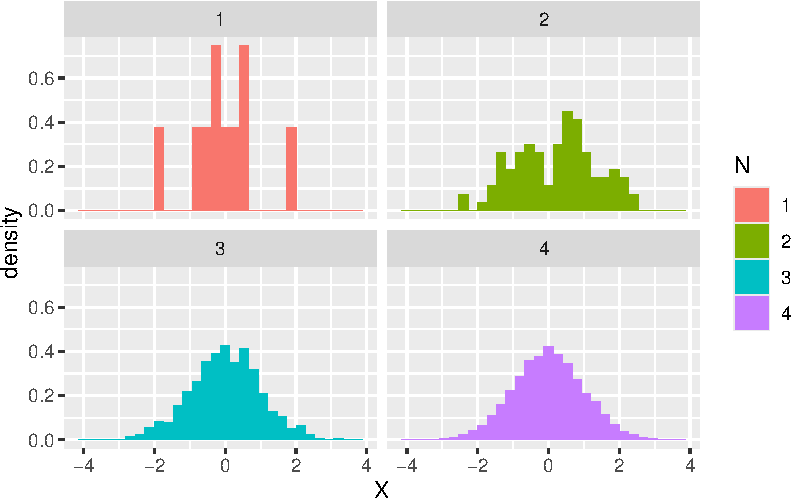
\includegraphics[keepaspectratio]{chapter06_files/figure-pdf/rnorm-1.pdf}}

これを見ると,最初の10個程度のヒストグラムは不規則な分布に見えるが,100,1000と増えるに従って徐々に正規分布の理論的形状に近似していくところがみて取れる。

Rにはポアソン分布や二項分布などに加え,統計に馴染みの深いt分布やF分布,\(\chi^2\)分布などの確率分布関数も実装されている。これらの分布はパラメタの値を聞いてもイメージしにくいところがあるかもしれないが,そのような時はパラメタを指定した上で乱数を大量に生成し,そのヒストグラムを描けば確率分布関数の形が眼に見えてくるため,より具体的に理解できるだろう。

実際,ベイズ統計学が昨今隆盛している一つの理由は,計算機科学の貢献によるところが大きい。\textbf{マルコフ連鎖モンテカルロ法}(MCMC法)と呼ばれる乱数発生技術は,明確な名前を持たないモデルによって作られる事後分布からでも,乱数を生成できる技術である。この分布は解析的に示すことは困難であるが,そこから乱数を生成し,そのヒストグラムを見ることで,形状を可視化できるのである。

また,この乱数利用法の利点は可視化だけではない。標準正規分布において,ある範囲の面積(=確率)が知りたいとする。たとえば,確率点-1.5から+1.5までの範囲の面積を求めたいとしよう。正規分布の数式はわかっているので,次のようにすればその面積は求められる。
\[ p = \int_{-1.5}^{+1.5} \frac{1}{\sqrt{2\pi}}e^{-\frac{x^2}{2}} dx \]

もちろん我々は\texttt{pnorm}関数を知っているので,次のようにして数値解を得ることができる。

\begin{Shaded}
\begin{Highlighting}[]
\FunctionTok{pnorm}\NormalTok{(}\SpecialCharTok{+}\FloatTok{1.5}\NormalTok{, }\AttributeTok{mean =} \DecValTok{0}\NormalTok{, }\AttributeTok{sd =} \DecValTok{1}\NormalTok{) }\SpecialCharTok{{-}} \FunctionTok{pnorm}\NormalTok{(}\SpecialCharTok{{-}}\FloatTok{1.5}\NormalTok{, }\AttributeTok{mean =} \DecValTok{0}\NormalTok{, }\AttributeTok{sd =} \DecValTok{1}\NormalTok{)}
\end{Highlighting}
\end{Shaded}

\begin{verbatim}
[1] 0.8663856
\end{verbatim}

同様のことは乱数を使って,次のように近似解を得ることができる。

\begin{Shaded}
\begin{Highlighting}[]
\NormalTok{x }\OtherTok{\textless{}{-}} \FunctionTok{rnorm}\NormalTok{(}\DecValTok{100000}\NormalTok{, }\AttributeTok{mean =} \DecValTok{0}\NormalTok{, }\AttributeTok{sd =} \DecValTok{1}\NormalTok{)}
\NormalTok{df }\OtherTok{\textless{}{-}} \FunctionTok{data.frame}\NormalTok{(}\AttributeTok{X =}\NormalTok{ x) }\SpecialCharTok{\%\textgreater{}\%}
  \CommentTok{\# 該当する範囲かどうかを判定する変数を作る}
  \FunctionTok{mutate}\NormalTok{(}\AttributeTok{FLG =} \FunctionTok{ifelse}\NormalTok{(X }\SpecialCharTok{\textgreater{}} \SpecialCharTok{{-}}\FloatTok{1.5} \SpecialCharTok{\&}\NormalTok{ X }\SpecialCharTok{\textless{}} \FloatTok{1.5}\NormalTok{, }\DecValTok{1}\NormalTok{, }\DecValTok{2}\NormalTok{)) }\SpecialCharTok{\%\textgreater{}\%}
  \FunctionTok{mutate}\NormalTok{(}\AttributeTok{FLG =} \FunctionTok{factor}\NormalTok{(FLG, }\AttributeTok{labels =} \FunctionTok{c}\NormalTok{(}\StringTok{"in"}\NormalTok{, }\StringTok{"out"}\NormalTok{)))}
\DocumentationTok{\#\# 計算}
\NormalTok{df }\SpecialCharTok{\%\textgreater{}\%}
  \FunctionTok{group\_by}\NormalTok{(FLG) }\SpecialCharTok{\%\textgreater{}\%}
  \FunctionTok{summarise}\NormalTok{(}\AttributeTok{n =} \FunctionTok{n}\NormalTok{()) }\SpecialCharTok{\%\textgreater{}\%}
  \FunctionTok{mutate}\NormalTok{(}\AttributeTok{prob =}\NormalTok{ n }\SpecialCharTok{/} \DecValTok{100000}\NormalTok{)}
\end{Highlighting}
\end{Shaded}

\begin{verbatim}
# A tibble: 2 x 3
  FLG       n  prob
  <fct> <int> <dbl>
1 in    86642 0.866
2 out   13358 0.134
\end{verbatim}

ここでは乱数を10,000個生成し,指定の範囲内に入るかどうか(入れば1,入らなければ2)を示すfactor型変数\texttt{FLG}を作った。この変数ごとに群分けして数を数え,総数で割ることで相対度数にする。確率は全体の中に占める相対的な面積の割合であり,今回当該領域の値が\texttt{0.866}と\texttt{pnorm}関数で算出した解とほぼ同等の値変えられている。

なお,次のようにすれば範囲の可視化も容易い。

\begin{Shaded}
\begin{Highlighting}[]
\DocumentationTok{\#\# 可視化}
\NormalTok{df }\SpecialCharTok{\%\textgreater{}\%}
  \FunctionTok{ggplot}\NormalTok{(}\FunctionTok{aes}\NormalTok{(}\AttributeTok{x =}\NormalTok{ X, }\AttributeTok{fill =}\NormalTok{ FLG)) }\SpecialCharTok{+}
  \FunctionTok{geom\_histogram}\NormalTok{(}\AttributeTok{binwidth =} \FloatTok{0.01}\NormalTok{)}
\end{Highlighting}
\end{Shaded}

\pandocbounded{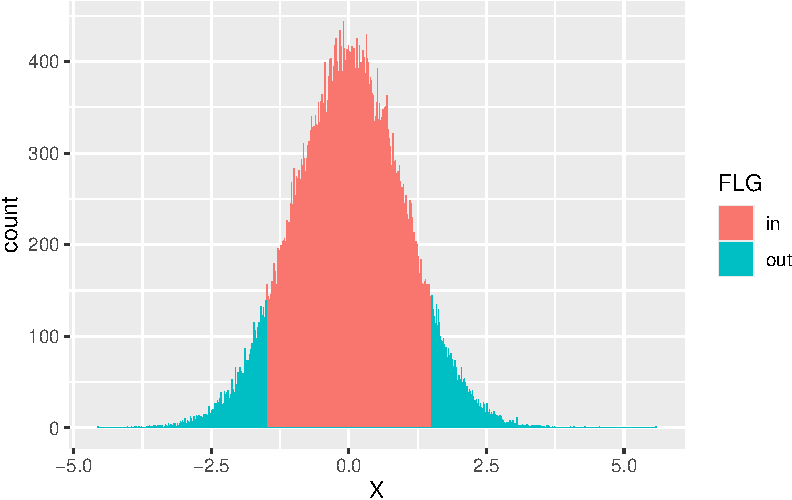
\includegraphics[keepaspectratio]{chapter06_files/figure-pdf/norm_vis-1.pdf}}

繰り返すが,確率分布の形がイメージできなかったり,解析的にその式を書き表すことが困難であった場合でも,具体的な数値にすることでヒストグラムで可視化でき,また近似的に確率計算ができている。

あくまでも近似に過ぎないのでその精度が信用できない,というひとは生成する乱数の数を10倍,100倍にすれば良い。昨今の計算機の計算能力において,その程度の増加はさほど計算料の負担にならない。複雑な積分計算が記述統計量(数え上げ)の問題になる点で,具体的に理解できるという利点は大きい。

さらに思いを馳せてほしいのだが,心理学者は心理学実験や調査によって,データを得る。しかしそれらは個人差や誤差を考え,確率変数だとされている。目の前の数件から数十件のデータであっても,正規分布に従うと仮定して統計的処理をおこなう。これは「乱数によって生成したデータ」に対して行うとしても本質的には同じである。すなわち,調査実験を行う前に,乱数によってシミュレーションしておくことができるのである。調査実験の本番一発勝負をする前に,自分の取ろうとしているデータがどのような性質を持ちうるかを具体的に確かめておくことは重要な試みであろう。

\section{練習問題;乱数を用いて}\label{ux7df4ux7fd2ux554fux984cux4e71ux6570ux3092ux7528ux3044ux3066}

正規乱数を用いて,次の値を近似計算してみよう。なお設定や解析的に算出した「真の値」と少数以下2位までの精度が得られるように工夫しよう。

\begin{enumerate}
\def\labelenumi{\arabic{enumi}.}
\tightlist
\item
  平均100,標準偏差8の正規分布の期待値。なお連続確率変数の期待値は次の式で表されます。\[E[X] = \int_{-\infty}^{\infty} x f(x) \, dx\]
  ここで\(x\)は確率変数を表し,\(f(x)\)は確率密度関数であり,確率密度関数の全定義域を積分することで得られます。正規分布の期待値は,平均パラメータに一致しますので,今回の真値は設定した\(100\)になります。
\item
  平均100,標準偏差3の正規分布の分散を計算してみよう。なお連続確率変数の分散は次の式で表されます。\[\sigma^2 = \int_{-\infty}^{\infty} (x - \mu)^2 f(x) \, dx\]
  ここで\(\mu\)は確率変数の期待値であり,正規分布の分散は,標準偏差パラメータの二乗に一致しますので,今回の真値は\(3^2 = 9\)です。
\item
  平均65,標準偏差10の正規分布に従う確率変数\(X\)の,\(90 < X < 110\)の面積。解析的に計算した結果は次の通りです。
\end{enumerate}

\begin{Shaded}
\begin{Highlighting}[]
\FunctionTok{pnorm}\NormalTok{(}\DecValTok{110}\NormalTok{, }\AttributeTok{mean =} \DecValTok{65}\NormalTok{, }\AttributeTok{sd =} \DecValTok{10}\NormalTok{) }\SpecialCharTok{{-}} \FunctionTok{pnorm}\NormalTok{(}\DecValTok{90}\NormalTok{, }\AttributeTok{mean =} \DecValTok{65}\NormalTok{, }\AttributeTok{sd =} \DecValTok{10}\NormalTok{)}
\end{Highlighting}
\end{Shaded}

\begin{verbatim}
[1] 0.006206268
\end{verbatim}

\begin{enumerate}
\def\labelenumi{\arabic{enumi}.}
\setcounter{enumi}{3}
\tightlist
\item
  平均10,標準偏差10の正規分布において,実現値が7以上になる確率。解析的に計算した結果は次の通りです。
\end{enumerate}

\begin{Shaded}
\begin{Highlighting}[]
\DecValTok{1} \SpecialCharTok{{-}} \FunctionTok{pnorm}\NormalTok{(}\DecValTok{7}\NormalTok{, }\AttributeTok{mean =} \DecValTok{10}\NormalTok{, }\AttributeTok{sd =} \DecValTok{10}\NormalTok{)}
\end{Highlighting}
\end{Shaded}

\begin{verbatim}
[1] 0.6179114
\end{verbatim}

\begin{enumerate}
\def\labelenumi{\arabic{enumi}.}
\setcounter{enumi}{4}
\tightlist
\item
  確率変数\(X,Y\)があります。\(X\)は平均10,SD10の正規分布,\(Y\)は平均5,SD8の正規分布に従うものとします。ここで,\(X\)と\(Y\)が独立であるとしたとき,和\(Z=X+Y\)の平均と分散が,もとの\(X,Y\)の平均の和,分散の和になっていることを,乱数を使って確認してください。
\end{enumerate}

\section{母集団と標本}\label{ux6bcdux96c6ux56e3ux3068ux6a19ux672c}

ここまで確率分布の性質を見るために乱数を利用する方法を見てきた。ここからは,推測統計学における確率分布の利用を考える。推測統計では,知りたい集団全体のことを\textbf{母集団population},そこから得られた一部のデータを\textbf{標本sample}と呼ぶのであった。標本の統計量を使って,母集団の性質を推論するのが推測統計/統計的推測である。母集団の特徴を表す統計量は\textbf{母数parameter}と呼ばれ,母平均,母分散など「母」の字をつけて母集団の情報であることを示す。同様に,標本の平均や分散も計算できるが,この時は標本平均,標本分散など「標本」をつけて明示的に違いを強調することもある。

乱数を使って具体的な例で見てみよう。ここに100人から構成される村があったとする。この村の人々の身長を測ってデータにしたとしよう。100個の適当な数字を考えるのは面倒なので,乱数で生成してこれに代える。

\begin{Shaded}
\begin{Highlighting}[]
\FunctionTok{set.seed}\NormalTok{(}\DecValTok{12345}\NormalTok{)}
\CommentTok{\# 100人分の身長データをつくる。小数点以下2桁を丸めた}
\NormalTok{Po }\OtherTok{\textless{}{-}} \FunctionTok{rnorm}\NormalTok{(}\DecValTok{100}\NormalTok{, }\AttributeTok{mean =} \DecValTok{150}\NormalTok{, }\AttributeTok{sd =} \DecValTok{10}\NormalTok{) }\SpecialCharTok{\%\textgreater{}\%} \FunctionTok{round}\NormalTok{(}\DecValTok{2}\NormalTok{)}
\FunctionTok{print}\NormalTok{(Po)}
\end{Highlighting}
\end{Shaded}

\begin{verbatim}
  [1] 155.86 157.09 148.91 145.47 156.06 131.82 156.30 147.24 147.16 140.81
 [11] 148.84 168.17 153.71 155.20 142.49 158.17 141.14 146.68 161.21 152.99
 [21] 157.80 164.56 143.56 134.47 134.02 168.05 145.18 156.20 156.12 148.38
 [31] 158.12 171.97 170.49 166.32 152.54 154.91 146.76 133.38 167.68 150.26
 [41] 161.29 126.20 139.40 159.37 158.54 164.61 135.87 155.67 155.83 136.93
 [51] 144.60 169.48 150.54 153.52 143.29 152.78 156.91 158.24 171.45 126.53
 [61] 151.50 136.57 155.53 165.90 144.13 131.68 158.88 165.93 155.17 137.04
 [71] 150.55 142.15 139.51 173.31 164.03 159.43 158.26 141.88 154.76 160.21
 [81] 156.45 160.43 146.96 174.77 159.71 168.67 156.72 146.92 155.37 158.25
 [91] 140.36 141.45 168.87 146.08 140.19 156.87 144.95 171.58 144.00 143.05
\end{verbatim}

この100人の村が母集団なので,母平均や母分散は次のようにして計算できる。

\begin{Shaded}
\begin{Highlighting}[]
\NormalTok{M }\OtherTok{\textless{}{-}} \FunctionTok{mean}\NormalTok{(Po)}
\NormalTok{V }\OtherTok{\textless{}{-}} \FunctionTok{mean}\NormalTok{((Po }\SpecialCharTok{{-}}\NormalTok{ M)}\SpecialCharTok{\^{}}\DecValTok{2}\NormalTok{)}
\CommentTok{\# 母平均}
\FunctionTok{print}\NormalTok{(M)}
\end{Highlighting}
\end{Shaded}

\begin{verbatim}
[1] 152.4521
\end{verbatim}

\begin{Shaded}
\begin{Highlighting}[]
\CommentTok{\# 母分散}
\FunctionTok{print}\NormalTok{(V)}
\end{Highlighting}
\end{Shaded}

\begin{verbatim}
[1] 123.0206
\end{verbatim}

さて,この村からランダムに10人の標本を得たとしよう。ベクトルの前から10人でも良いが,Rにはサンプリングをする関数\texttt{sample}があるのでこれを活用する。

\begin{Shaded}
\begin{Highlighting}[]
\NormalTok{s1 }\OtherTok{\textless{}{-}} \FunctionTok{sample}\NormalTok{(Po, }\AttributeTok{size =} \DecValTok{10}\NormalTok{)}
\NormalTok{s1}
\end{Highlighting}
\end{Shaded}

\begin{verbatim}
 [1] 164.61 155.86 136.93 143.29 160.43 168.87 151.50 155.17 153.71 135.87
\end{verbatim}

この\texttt{s1}が手元のデータである。心理学の実験でデータを得る,というのはこのように全体に対してごく一部だけ取り出したものになる。このサンプルの平均や分散は標本平均,標本分散である。

\begin{Shaded}
\begin{Highlighting}[]
\NormalTok{m1 }\OtherTok{\textless{}{-}} \FunctionTok{mean}\NormalTok{(s1)}
\NormalTok{v1 }\OtherTok{\textless{}{-}} \FunctionTok{mean}\NormalTok{((s1 }\SpecialCharTok{{-}} \FunctionTok{mean}\NormalTok{(s1))}\SpecialCharTok{\^{}}\DecValTok{2}\NormalTok{)}
\CommentTok{\# 標本平均}
\FunctionTok{print}\NormalTok{(m1)}
\end{Highlighting}
\end{Shaded}

\begin{verbatim}
[1] 152.624
\end{verbatim}

\begin{Shaded}
\begin{Highlighting}[]
\CommentTok{\# 標本分散}
\FunctionTok{print}\NormalTok{(v1)}
\end{Highlighting}
\end{Shaded}

\begin{verbatim}
[1] 110.2049
\end{verbatim}

今回,母平均は152.4521で標本平均は152.624である。実際に知りうる値は標本の値だけなので,標本平均152.624を得たら,母平均も152.624に近い値だろうな,と推測するのはおかしなことではないだろう。しかし標本平均は,標本の取り方によって毎回変わるものである。試しにもう一つ,標本をとったとしよう。

\begin{Shaded}
\begin{Highlighting}[]
\NormalTok{s2 }\OtherTok{\textless{}{-}} \FunctionTok{sample}\NormalTok{(Po, }\AttributeTok{size =} \DecValTok{10}\NormalTok{)}
\NormalTok{s2}
\end{Highlighting}
\end{Shaded}

\begin{verbatim}
 [1] 154.76 135.87 143.05 171.45 136.57 170.49 156.87 158.25 155.17 155.20
\end{verbatim}

\begin{Shaded}
\begin{Highlighting}[]
\NormalTok{m2 }\OtherTok{\textless{}{-}} \FunctionTok{mean}\NormalTok{(s2)}
\NormalTok{v2 }\OtherTok{\textless{}{-}} \FunctionTok{mean}\NormalTok{((s2 }\SpecialCharTok{{-}} \FunctionTok{mean}\NormalTok{(s2))}\SpecialCharTok{\^{}}\DecValTok{2}\NormalTok{)}
\CommentTok{\# 標本平均その2}
\FunctionTok{print}\NormalTok{(m2)}
\end{Highlighting}
\end{Shaded}

\begin{verbatim}
[1] 153.768
\end{verbatim}

今回の標本平均は153.768になった。このデータが得られたら,諸君は母平均が「153.768に近い値だろうな」と推測するに違いない。標本1の152.624と標本2の153.768を比べると,前者の方が正解152.4521に近い(その差はそれぞれ-0.1719と-1.3159である)。つまり,標本の取り方によっては当たり外れがあるということである。データをとって研究していても,仮説を支持する結果なのかそうでないのかは,こうした確率的揺らぎの下にある。

つまり,\textbf{標本は確率変数であり,標本統計量も確率的に変わりうる}ものである。標本統計量でもって母数を推定するときは,標本統計量の性質や標本統計量が従う確率分布を知っておく必要がある。以下では母数の推定に望ましい性質を持つ推定量の望ましい性質をみていこう。

\section{一致性}\label{ux4e00ux81f4ux6027}

最も単純には,標本統計量が母数に近ければ近いほど,できれば一致してくれれば喜ばしい。先ほどの例では100人の村から10人しか取り出さなかったが,もし20人,30人とサンプルサイズが大きくなると母数に近づいていくことが予想できる。この性質のことを\textbf{一致性}consistencyといい,推定量が持っていてほしい性質のひとつである。幸い,標本平均は母平均に対して一致性を持っている。

このことを確認してみよう。サンプルサイズを様々に変えて計算してみれば良い。例として,平均50,SD10の正規分布からサンプルサイズを2から1000まで増やしていくことにしよう。サンプルを取り出すことを,乱数生成に置き換えてその平均を計算していくこととする。

\begin{Shaded}
\begin{Highlighting}[]
\FunctionTok{set.seed}\NormalTok{(}\DecValTok{12345}\NormalTok{)}
\NormalTok{sample\_size }\OtherTok{\textless{}{-}} \FunctionTok{seq}\NormalTok{(}\AttributeTok{from =} \DecValTok{2}\NormalTok{, }\AttributeTok{to =} \DecValTok{1000}\NormalTok{, }\AttributeTok{by =} \DecValTok{10}\NormalTok{)}
\CommentTok{\# 平均値を格納するオブジェクトを初期化}
\NormalTok{sample\_mean }\OtherTok{\textless{}{-}} \FunctionTok{rep}\NormalTok{(}\DecValTok{0}\NormalTok{, }\FunctionTok{length}\NormalTok{(sample\_size))}
\CommentTok{\# 反復}
\ControlFlowTok{for}\NormalTok{ (i }\ControlFlowTok{in} \DecValTok{1}\SpecialCharTok{:}\FunctionTok{length}\NormalTok{(sample\_size)) \{}
\NormalTok{  sample\_mean[i] }\OtherTok{\textless{}{-}} \FunctionTok{rnorm}\NormalTok{(sample\_size[i], }\AttributeTok{mean =} \DecValTok{50}\NormalTok{, }\AttributeTok{sd =} \DecValTok{10}\NormalTok{) }\SpecialCharTok{\%\textgreater{}\%}
    \FunctionTok{mean}\NormalTok{()}
\NormalTok{\}}

\CommentTok{\# 可視化}
\FunctionTok{data.frame}\NormalTok{(}\AttributeTok{size =}\NormalTok{ sample\_size, }\AttributeTok{M =}\NormalTok{ sample\_mean) }\SpecialCharTok{\%\textgreater{}\%}
  \FunctionTok{ggplot}\NormalTok{(}\FunctionTok{aes}\NormalTok{(}\AttributeTok{x =}\NormalTok{ size, }\AttributeTok{y =}\NormalTok{ M)) }\SpecialCharTok{+}
  \FunctionTok{geom\_point}\NormalTok{() }\SpecialCharTok{+}
  \FunctionTok{geom\_line}\NormalTok{() }\SpecialCharTok{+}
  \FunctionTok{geom\_hline}\NormalTok{(}\AttributeTok{yintercept =} \DecValTok{50}\NormalTok{, }\AttributeTok{color =} \StringTok{"red"}\NormalTok{)}
\end{Highlighting}
\end{Shaded}

\pandocbounded{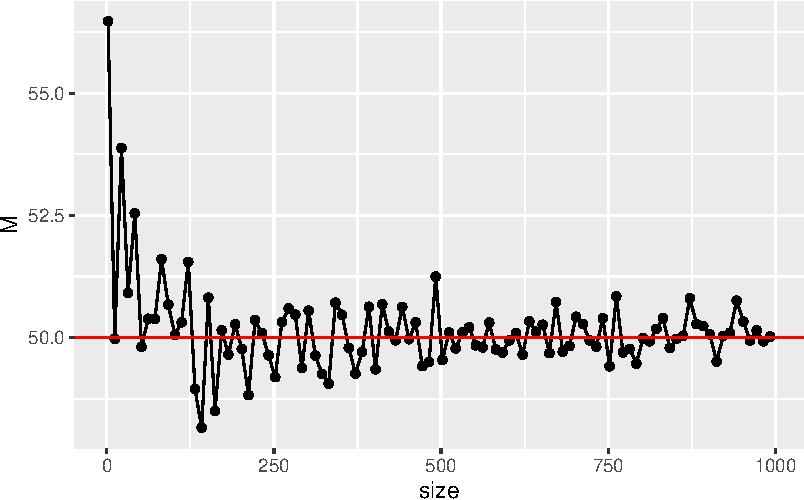
\includegraphics[keepaspectratio]{chapter06_files/figure-pdf/consistency-1.pdf}}

このようにサンプルサイズが増えていくにつれて,真値の50に近づいていくことが見て取れる。母集団分布の形状やパラメータ,サンプルサイズなどを変えて確認してみよう。

\section{不偏性}\label{ux4e0dux504fux6027}

推定量は確率変数であり,確率分布でその性質を記述することができる。標本統計量の従う確率分布のことを\textbf{標本分布}と呼ぶが,標本分布の確率密度関数がわかっているなら,その期待値や分散も計算できるだろう。推定量の期待値(平均)が母数に一致することも,推定量の望ましい性質の一つであり,この性質のことを\textbf{不偏性}unbiasednessという。

心理統計を学ぶ時に初学者を苛立たせるステップの一つとして,分散の計算の時にサンプルサイズ\(n\)ではなく\(n-1\)で割る,という操作がある。これは不偏分散といって標本分散とは違うのだが,前者が不偏性を持っているのに対し,後者がそうでないからである。これを乱数を使って確認してみよう。

平均50,SD10(母分散\(10^2=100\))の母集団から,サンプルサイズ\(n=20\)の標本を繰り返し得る。これはサイズ20の乱数生成で行う。各標本に対して標本分散と不偏分散を計算し,その平均(標本統計量の期待値)を計算してみよう。

\begin{Shaded}
\begin{Highlighting}[]
\NormalTok{iter }\OtherTok{\textless{}{-}} \DecValTok{5000}
\NormalTok{vars }\OtherTok{\textless{}{-}} \FunctionTok{rep}\NormalTok{(}\DecValTok{0}\NormalTok{, iter)}
\NormalTok{unbiased\_vars }\OtherTok{\textless{}{-}} \FunctionTok{rep}\NormalTok{(}\DecValTok{0}\NormalTok{, iter)}

\DocumentationTok{\#\# 乱数の生成と計算}
\FunctionTok{set.seed}\NormalTok{(}\DecValTok{12345}\NormalTok{)}
\ControlFlowTok{for}\NormalTok{ (i }\ControlFlowTok{in} \DecValTok{1}\SpecialCharTok{:}\NormalTok{iter) \{}
\NormalTok{  sample }\OtherTok{\textless{}{-}} \FunctionTok{rnorm}\NormalTok{(}\AttributeTok{n =} \DecValTok{20}\NormalTok{, }\AttributeTok{mean =} \DecValTok{50}\NormalTok{, }\AttributeTok{sd =} \DecValTok{10}\NormalTok{)}
\NormalTok{  vars[i] }\OtherTok{\textless{}{-}} \FunctionTok{mean}\NormalTok{((sample }\SpecialCharTok{{-}} \FunctionTok{mean}\NormalTok{(sample))}\SpecialCharTok{\^{}}\DecValTok{2}\NormalTok{)}
\NormalTok{  unbiased\_vars[i] }\OtherTok{\textless{}{-}} \FunctionTok{var}\NormalTok{(sample)}
\NormalTok{\}}

\DocumentationTok{\#\# 期待値}
\FunctionTok{mean}\NormalTok{(vars)}
\end{Highlighting}
\end{Shaded}

\begin{verbatim}
[1] 95.08531
\end{verbatim}

\begin{Shaded}
\begin{Highlighting}[]
\FunctionTok{mean}\NormalTok{(unbiased\_vars)}
\end{Highlighting}
\end{Shaded}

\begin{verbatim}
[1] 100.0898
\end{verbatim}

標本分散を計算したオブジェクト\texttt{vars}の平均すなわち期待値は95.0853144であり,設定した値(真値)の100からは幾分はなれている。これに対して,Rの埋め込み関数である\texttt{var}をつかった不偏分散の平均すなわち期待値は100.0898047であり,母分散の推定量としてはこちらの方が好ましいことがわかる。このように標本分散にはバイアスが生じることがわかっているので,あらかじめバイアスを補正するために元の計算式を修正していたのである。この説明で,苛立ちを感じていた人の溜飲が下がればよいのだが。

他にも推定量の望ましい性質として有効性efficacyがあるが,詳細は
\textcite{kosugi2023}
を参照してほしい。この本には正規分布以外の例や,相関係数など他の標本統計量の例なども載っているが,いずれも乱数生成による近似で理解を進めるものである。諸君も数理統計的な説明に疲れたなら,ぜひ参考にしてもらいたい。

\section{信頼区間}\label{ux4fe1ux983cux533aux9593}

標本統計量は確率変数であり,標本を取るたびに変わる。標本を取るときに入る確率的ゆらぎによるからで,標本平均は一致性,不偏性という望ましい性質を持ってはいるが,標本平均\(=\)母平均とはならない。

標本平均という確率変数の実現値一点でもって,母平均を推測することは,母平均を推測する上ではほぼ確実に外れるギャンブルである。そこで母数に対してある幅でもって推定することを考えよう。

たとえば平均50,標準偏差10の標準正規分布を母集団分布とし,サンプルサイズ10の標本をとり,その標本平均を母平均の推定値としよう(点推定)。同時に,その推定値に少し幅を持たせ,たとえば標本平均\(\pm 5\)の\textbf{区間推定}をしたとする。この時,真値\(0\)を正しく推測できる確率を,反復乱数生成のシミュレーションで確かめてみよう。

\begin{Shaded}
\begin{Highlighting}[]
\NormalTok{iter }\OtherTok{\textless{}{-}} \DecValTok{10000}
\NormalTok{n }\OtherTok{\textless{}{-}} \DecValTok{10}
\NormalTok{mu }\OtherTok{\textless{}{-}} \DecValTok{50}
\NormalTok{SD }\OtherTok{\textless{}{-}} \DecValTok{10}

\CommentTok{\# 平均値を格納しておくオブジェクト}
\NormalTok{m }\OtherTok{\textless{}{-}} \FunctionTok{rep}\NormalTok{(}\DecValTok{0}\NormalTok{, iter)}

\FunctionTok{set.seed}\NormalTok{(}\DecValTok{12345}\NormalTok{)}
\ControlFlowTok{for}\NormalTok{ (i }\ControlFlowTok{in} \DecValTok{1}\SpecialCharTok{:}\NormalTok{iter) \{}
  \CommentTok{\# サンプリングし,標本統計量を保存}
\NormalTok{  sample }\OtherTok{\textless{}{-}} \FunctionTok{rnorm}\NormalTok{(n, }\AttributeTok{mean =}\NormalTok{ mu, }\AttributeTok{sd =}\NormalTok{ SD)}
\NormalTok{  m[i] }\OtherTok{\textless{}{-}} \FunctionTok{mean}\NormalTok{(sample)}
\NormalTok{\}}

\NormalTok{result.df }\OtherTok{\textless{}{-}} \FunctionTok{data.frame}\NormalTok{(}\AttributeTok{m =}\NormalTok{ m) }\SpecialCharTok{\%\textgreater{}\%}
  \CommentTok{\# 推定が一致するとTRUE,外れるとFALSEになる変数を作る}
  \FunctionTok{mutate}\NormalTok{(}
    \AttributeTok{point\_estimation =} \FunctionTok{ifelse}\NormalTok{(m }\SpecialCharTok{==}\NormalTok{ mu, }\ConstantTok{TRUE}\NormalTok{, }\ConstantTok{FALSE}\NormalTok{),}
    \AttributeTok{interval\_estimation =} \FunctionTok{ifelse}\NormalTok{(m }\SpecialCharTok{{-}} \DecValTok{5} \SpecialCharTok{\textless{}=}\NormalTok{ mu }\SpecialCharTok{\&}\NormalTok{ mu }\SpecialCharTok{\textless{}=}\NormalTok{ m }\SpecialCharTok{+} \DecValTok{5}\NormalTok{, }\ConstantTok{TRUE}\NormalTok{, }\ConstantTok{FALSE}\NormalTok{)}
\NormalTok{  ) }\SpecialCharTok{\%\textgreater{}\%}
  \FunctionTok{summarise}\NormalTok{(}
    \AttributeTok{n1 =} \FunctionTok{sum}\NormalTok{(point\_estimation),}
    \AttributeTok{n2 =} \FunctionTok{sum}\NormalTok{(interval\_estimation),}
    \AttributeTok{prob1 =} \FunctionTok{mean}\NormalTok{(point\_estimation),}
    \AttributeTok{prob2 =} \FunctionTok{mean}\NormalTok{(interval\_estimation)}
\NormalTok{  ) }\SpecialCharTok{\%\textgreater{}\%}
  \FunctionTok{print}\NormalTok{()}
\end{Highlighting}
\end{Shaded}

\begin{verbatim}
  n1   n2 prob1 prob2
1  0 8880     0 0.888
\end{verbatim}

結果からわかるように,点推定値は一度も正しく母数を当てていない。これは当然で,実数でやる以上小数点以下どこかでズレてしまうことがあるからで,精度を無視すると一致することはあり得ないのである。これに対して幅を持った予測の場合は,\ensuremath{10^{4}}回の試行のうち8880回はその区間内に真値を含んでおり,その正答率は88.8\%である。

区間推定において正答率を100\%にするためには,その区間を無限に広げなければならない(母平均の推定の場合)。これは実質的に何も推定していないことに等しいので,5\%程度の失敗を認めよう,95\%
の正答率で区間推定しようというのが習わしになっている。この区間のことを95\%の\textbf{信頼区間}confidence
intervalという。

\subsection{正規母集団分布の母分散が明らかな場合の信頼区間}\label{ux6b63ux898fux6bcdux96c6ux56e3ux5206ux5e03ux306eux6bcdux5206ux6563ux304cux660eux3089ux304bux306aux5834ux5408ux306eux4fe1ux983cux533aux9593}

上のシミュレーションを応用して,区間推定が正当する確率が95\%になるまで区間を調整して行ってもよいが,さすがにそれは面倒なので,推測統計学によって明らかになっている性質を紹介しよう。

母集団が正規分布に従い,その母平均が\(\mu\),母分散が\(\sigma^2\)であることがわかっている場合,標本平均の従う分布は平均\(\mu\),
分散\(\frac{\sigma^2}{n}\)(標準偏差\(\frac{\sigma}{\sqrt{n}})\)の正規分布であることがわかっている。

標準正規分布の95\%区間は,次の通り約\(\pm 1.96\)である。

\begin{Shaded}
\begin{Highlighting}[]
\CommentTok{\# 両端から2.5\%ずつ取り除くと}
\FunctionTok{qnorm}\NormalTok{(}\FloatTok{0.025}\NormalTok{)}
\end{Highlighting}
\end{Shaded}

\begin{verbatim}
[1] -1.959964
\end{verbatim}

\begin{Shaded}
\begin{Highlighting}[]
\FunctionTok{qnorm}\NormalTok{(}\FloatTok{0.975}\NormalTok{)}
\end{Highlighting}
\end{Shaded}

\begin{verbatim}
[1] 1.959964
\end{verbatim}

これらを合わせると,標本平均が\(\bar{X}\)であったとき,95\%信頼区間は標準偏差を1.96倍して,次のようになる。

\[ \bar{X} - 1.96 \frac{\sigma}{\sqrt{n}} \le \mu \le \bar{X} + 1.96 \frac{\sigma}{\sqrt{n}} \]

先ほどの数値例を応用して,これを確かめてみよう。95%ちかい割合で,区間内に真値が含んでいることがわかる。

\begin{Shaded}
\begin{Highlighting}[]
\NormalTok{interval }\OtherTok{\textless{}{-}} \FloatTok{1.96} \SpecialCharTok{*}\NormalTok{ SD }\SpecialCharTok{/} \FunctionTok{sqrt}\NormalTok{(n)}
\NormalTok{result.df2 }\OtherTok{\textless{}{-}} \FunctionTok{data.frame}\NormalTok{(}\AttributeTok{m =}\NormalTok{ m) }\SpecialCharTok{\%\textgreater{}\%}
  \CommentTok{\# 推定が一致するとTRUE,外れるとFALSEになる変数を作る}
  \FunctionTok{mutate}\NormalTok{(}
    \AttributeTok{interval\_estimation =} \FunctionTok{ifelse}\NormalTok{(m }\SpecialCharTok{{-}}\NormalTok{ interval }\SpecialCharTok{\textless{}=}\NormalTok{ mu }\SpecialCharTok{\&}\NormalTok{ mu }\SpecialCharTok{\textless{}=}\NormalTok{ m }\SpecialCharTok{+}\NormalTok{ interval, }\ConstantTok{TRUE}\NormalTok{, }\ConstantTok{FALSE}\NormalTok{)}
\NormalTok{  ) }\SpecialCharTok{\%\textgreater{}\%}
  \FunctionTok{summarise}\NormalTok{(}
    \AttributeTok{prob =} \FunctionTok{mean}\NormalTok{(interval\_estimation)}
\NormalTok{  ) }\SpecialCharTok{\%\textgreater{}\%}
  \FunctionTok{print}\NormalTok{()}
\end{Highlighting}
\end{Shaded}

\begin{verbatim}
    prob
1 0.9498
\end{verbatim}

\subsection{正規母集団分布の母分散が不明な場合の信頼区間}\label{ux6b63ux898fux6bcdux96c6ux56e3ux5206ux5e03ux306eux6bcdux5206ux6563ux304cux4e0dux660eux306aux5834ux5408ux306eux4fe1ux983cux533aux9593}

先ほどの例では母分散がわかっている場合の例であったが,母平均や母分散がわかっていれば推測する必要はないわけで,実践的には母分散がわからない場合の推定が必要になってくる。幸いにしてそのような場合,すなわち母分散を不偏分散(標本統計量)で置き換えた場合は,標本平均が自由度\(n-1\)のt分布に従うことがわかっている。(詳細は
\textcite{kosugi2023} を参照)
ただその場合,標準正規分布のように95\%区間が\(\pm 1.96\)に限らず,サンプルサイズに応じてt分布の形が変わるから,それを考慮して以下の式で信頼区間を算出する。
\[ \bar{X} + T_{0.025}\frac{U}{\sqrt{n}} \le \mu \le \bar{X} + T_{0.975}\frac{U}{\sqrt{n}} \]

ここで\(T_{0.025}\)はt分布の2.5パーセンタイル,\(T_{0.975}\)は97.5パーセンタイルを指す。t分布は(平均が0であれば)左右対称なので,\(T_{0.025}=-T_{0.975}\)と考えても良い。また\(U^2\)は不偏分散である(\(U\)はその平方根)。

これも乱数による近似計算で確認しておこう。同じく95%ちかい割合で,区間内に真値が含まれていることがわかる。

\begin{Shaded}
\begin{Highlighting}[]
\CommentTok{\# シミュレーションの設定}
\NormalTok{iter }\OtherTok{\textless{}{-}} \DecValTok{10000}
\NormalTok{n }\OtherTok{\textless{}{-}} \DecValTok{10}
\NormalTok{mu }\OtherTok{\textless{}{-}} \DecValTok{50}
\NormalTok{SD }\OtherTok{\textless{}{-}} \DecValTok{10}

\CommentTok{\# 平均値を格納しておくオブジェクト}
\NormalTok{m }\OtherTok{\textless{}{-}} \FunctionTok{rep}\NormalTok{(}\DecValTok{0}\NormalTok{, iter)}
\NormalTok{interval }\OtherTok{\textless{}{-}} \FunctionTok{rep}\NormalTok{(}\DecValTok{0}\NormalTok{, iter)}

\FunctionTok{set.seed}\NormalTok{(}\DecValTok{12345}\NormalTok{)}
\ControlFlowTok{for}\NormalTok{ (i }\ControlFlowTok{in} \DecValTok{1}\SpecialCharTok{:}\NormalTok{iter) \{}
  \CommentTok{\# サンプリングし,標本統計量を保存}
\NormalTok{  sample }\OtherTok{\textless{}{-}} \FunctionTok{rnorm}\NormalTok{(n, }\AttributeTok{mean =}\NormalTok{ mu, }\AttributeTok{sd =}\NormalTok{ SD)}
\NormalTok{  m[i] }\OtherTok{\textless{}{-}} \FunctionTok{mean}\NormalTok{(sample)}
\NormalTok{  U }\OtherTok{\textless{}{-}} \FunctionTok{sqrt}\NormalTok{(}\FunctionTok{var}\NormalTok{(sample)) }\CommentTok{\# sd(sample)でも同じ}
\NormalTok{  interval[i] }\OtherTok{\textless{}{-}} \FunctionTok{qt}\NormalTok{(}\AttributeTok{p =} \FloatTok{0.975}\NormalTok{, }\AttributeTok{df =}\NormalTok{ n }\SpecialCharTok{{-}} \DecValTok{1}\NormalTok{) }\SpecialCharTok{*}\NormalTok{ U }\SpecialCharTok{/} \FunctionTok{sqrt}\NormalTok{(n)}
\NormalTok{\}}

\NormalTok{result.df }\OtherTok{\textless{}{-}} \FunctionTok{data.frame}\NormalTok{(}\AttributeTok{m =}\NormalTok{ m, }\AttributeTok{interval =}\NormalTok{ interval) }\SpecialCharTok{\%\textgreater{}\%}
  \CommentTok{\# 推定が一致するとTRUE,外れるとFALSEになる変数を作る}
  \FunctionTok{mutate}\NormalTok{(}
    \AttributeTok{interval\_estimation =} \FunctionTok{ifelse}\NormalTok{(m }\SpecialCharTok{{-}}\NormalTok{ interval }\SpecialCharTok{\textless{}=}\NormalTok{ mu }\SpecialCharTok{\&}\NormalTok{ mu }\SpecialCharTok{\textless{}=}\NormalTok{ m }\SpecialCharTok{+}\NormalTok{ interval, }\ConstantTok{TRUE}\NormalTok{, }\ConstantTok{FALSE}\NormalTok{)}
\NormalTok{  ) }\SpecialCharTok{\%\textgreater{}\%}
  \FunctionTok{summarise}\NormalTok{(}
    \AttributeTok{prob =} \FunctionTok{mean}\NormalTok{(interval\_estimation)}
\NormalTok{  ) }\SpecialCharTok{\%\textgreater{}\%}
  \FunctionTok{print}\NormalTok{()}
\end{Highlighting}
\end{Shaded}

\begin{verbatim}
    prob
1 0.9482
\end{verbatim}

\section{課題}\label{ux8ab2ux984c-4}

\begin{enumerate}
\def\labelenumi{\arabic{enumi}.}
\tightlist
\item
  算術平均\(M = \frac{1}{n}\sum x_i\)が一致推定量であることが示されましたが,調和平均\(HM = \frac{n}{\sum \frac{1}{x_i}}\)や幾何平均\(GM = (\prod x_i)^{\frac{1}{n}} = \exp(\frac{1}{n}\sum \log(x_i)))\)はどうでしょうか。シミュレーションで確かめてみましょう。
\item
  サンプルサイズ\(n\)が大きくなるほど,標本平均が母平均に近づくという性質は正規分布以外でも成立するでしょうか。自由度\(\nu = 3\)のt分布を使って,シミュレーションで確認してみましょう。なおt分布の乱数は\texttt{rt()}で生成でき,非心度パラメータ\texttt{ncp}を指定しなければその平均は0です。
\item
  t分布の自由度\(\nu\)が極めて大きい時は,標準正規分布に一致することがわかっています。\texttt{rt()}関数を使って自由度が10,50,100のときの乱数を1000個生成し,ヒストグラムを書いてその形状を確認しましょう。また乱数の平均と標本標準偏差を計算し,標準正規分布に近づくことを確認しましょう。
\item
  平均が50,標準偏差が10の正規分布からサンプルサイズ20の乱数を10000個生成し,quantile関数をつかって95%信頼区間をシミュレートしてください。理論値と比較して確認してください。
\item
  平均が100,標準偏差が15の正規分布から抽出された標本について,サンプルサイズを10,100,1000と変えたときの標本平均の95\%信頼区間の幅を比較してください。
\end{enumerate}

\bookmarksetup{startatroot}

\chapter{統計的仮説検定(Null Hypothesis Statistical
Testing)}\label{ux7d71ux8a08ux7684ux4eeeux8aacux691cux5b9anull-hypothesis-statistical-testing}

帰無仮説検定は,心理学における統計の利用シーンの代表的なものだろう。
その手順は形式化されており,統計パッケージによってはデータの種類を指定するだけで自動的に結果の記述までしてくれるものもあるほどである。誰がやっても同じ結果になり,また,機械的に手続きを自動化できることは大きな利点ではある。欠点は,初学者がそのメカニズムを十分に理解せずに誤った結果を得たり,悪意のある利用者が自分に都合の良い数字を出させたりすることにある。科学的営みは悪意をもった実践者を想定しておらず,もしそのような悪例が露見した場合には事後的に摘発・対処するしかない。しかし残念なことながら,初学者の浅慮や意図せぬ悪用も多くみられる。

心理学において,先行研究の結果が再現しないことを再現性問題というが,そのひとつは統計的手法の誤った使い方にあるとされる\autocite{Ikeda2016}。改めて,丁寧に帰無仮説検定の手続きやロジックを見ていくことにしよう。

\section{帰無仮説検定の理屈と手続き}\label{ux5e30ux7121ux4eeeux8aacux691cux5b9aux306eux7406ux5c48ux3068ux624bux7d9aux304d}

\subsection{帰無仮説検定の目的}\label{ux5e30ux7121ux4eeeux8aacux691cux5b9aux306eux76eeux7684}

帰無仮説検定は,実験や調査で得たデータから得られた知見が意味のあるものかどうか,母集団の性質として一般化可能かどうかを判定するための枠組みである。手法と判断基準が明確なゲームの一種だと考えたよう。というのも,帰無仮説検定は\textbf{有意水準}という基準を設けて,\textbf{帰無仮説}と\textbf{対立仮説}という2つの考え方(モデル)を対決させ,勝敗を決するものだからである。勝敗を決するとしたのは,帰無仮説と対立仮説は排他的な関係にあるからであり,どちらも正しいとかどちらも間違っているという結末にはならないからである。ただし,あくまでも推測統計的なロジックに基づく判定であるから,判定結果にも確率的な要素が含まれる。本当は帰無仮説が正しい時に,間違って「対立仮説が正しい」と判定してしまう確率はゼロではない。逆に帰無仮説が正しくない時に,間違って「対立仮説が正しくない(帰無仮説が正しい)」と判定してしまう可能性もある。前者を\textbf{タイプ1エラー},後者を\textbf{タイプ2エラー}という。どちらの確率もゼロであってほしいが,そうはならないので,前者を\(\alpha\),後者を\(\beta\)としたときに,それぞれを一定の水準以下に抑えたい。この目的のために手順を整え,一般化したのが帰無仮説検定である。なお,先に述べた有意水準は,この\(\alpha\)の許容される水準であり,心理学では一般に5\%に設定する。

このように帰無仮説検定という考え方は,エラーの統制が本来の狙いであるから,「有意になるように工夫する」という発想は根本的に間違っている。また,統計的推定という数学的手続きに,人間が納得しやすい判定を下すという人為的手続きが組み合わさったものであるから,帰無仮説検定の結果に過剰な意味を持たせたり一喜一憂したりすることがないように注意しよう。

\subsection{帰無仮説検定の手続き}\label{ux5e30ux7121ux4eeeux8aacux691cux5b9aux306eux624bux7d9aux304d}

帰無仮説検定の手続きを一般化すれば,次のようになる。

\begin{enumerate}
\def\labelenumi{\arabic{enumi}.}
\tightlist
\item
  帰無仮説と対立仮説を設定する。
\item
  検定統計量を選択する。
\item
  判定基準を決定する。
\item
  検定統計量を計算する。
\item
  判定する。
\end{enumerate}

帰無仮説検定は,群間の平均値に差があるかどうか,相関係数に統計的な意味があるかどうかといった事例に対して適用される。
当然のことながら,これは標本から母集団を推定するという文脈における話で,物理学的な真偽を理論的に判断するとか,全数調査のように母集団全体の情報が手に入る場合といった場合の話ではない。また,標本のサンプルサイズが小さく,標本統計量の信頼区間が大きいことから,枠組みなしには判定できないという背景があることも再確認しておこう。

母集団の状態がわからないので,仮説を設定する。帰無仮説Null
Hypothesisは空っぽの仮説という意味で,母平均差がない(差がゼロ,\(\mu_1 - \mu_2 = 0\))とか,母相関がゼロ(\(\rho = 0\))である,とされる。対立仮説Alternative
Hypothesisは帰無仮説と排他的な関係にある仮説としてつくられるから,「差が無くはない(\(\mu_1 - \mu_2 \neq 0\))」「相関がゼロではない(\(\rho \neq 0\))」という表現になる。なぜ帰無仮説がゼロであることから始められるかといえば,ふたつの排他的な仮説を考えた時にゼロでない状態というのは無数にあり得るので,仮説として特定できないからである(差が1のとき,1.1のとき,1.11のとき・・・と延々と検定し続けるわけにもいくまい)。

検定統計量の選択は,二群の平均値差のときは\(t\),三群以上の時は\(F\),相関係数の検定も\(t\),と天下り的に示されることが一般的である。もちろんこれらの統計量が選ばれるのは,数理統計的な論拠に基づいている。判定基準は5\%水準とすることが一般的だし,検定統計量の計算はアルゴリズムに沿って機械的に可能である。判定は客観的な指標に基づいて行われるから,「どの状況でどのような帰無仮説をおくか」が類型化できれば,この手続き全体が自動的に進められる。

しかしここでは改めて,丁寧に手順を追いながらみてみよう。

\section{相関係数の検定}\label{ux76f8ux95a2ux4fc2ux6570ux306eux691cux5b9a}

ここでは相関係数の検定を例に取り上げる。俗に「無相関検定」と呼ばれるように,相関がどれほど大きいとかどれほど意味があるということをチェックするのでは無く,無相関ではない,ということをチェックする。もちろん標本相関は計算してゼロでなければ,それは無相関ではない。ここで考えたいのは,母相関がゼロではないということである。言い換えると,母相関がゼロの状態であっても,標本相関がゼロでないことは,小標本のサンプリングという背景のもとでは当然のことである。

確認してみよう。まず,無相関なデータセットを作ることを考える。Rの\texttt{MASS}パッケージを使い,多変量正規分布の確率分布関数から乱数を生成しよう。

\begin{Shaded}
\begin{Highlighting}[]
\NormalTok{pacman}\SpecialCharTok{::}\FunctionTok{p\_load}\NormalTok{(MASS)}
\FunctionTok{set.seed}\NormalTok{(}\DecValTok{12345}\NormalTok{)}
\NormalTok{N }\OtherTok{\textless{}{-}} \DecValTok{100000}
\NormalTok{X }\OtherTok{\textless{}{-}} \FunctionTok{mvrnorm}\NormalTok{(N,}
  \AttributeTok{mu =} \FunctionTok{c}\NormalTok{(}\DecValTok{0}\NormalTok{, }\DecValTok{0}\NormalTok{),}
  \AttributeTok{Sigma =} \FunctionTok{matrix}\NormalTok{(}\FunctionTok{c}\NormalTok{(}\DecValTok{1}\NormalTok{, }\DecValTok{0}\NormalTok{, }\DecValTok{0}\NormalTok{, }\DecValTok{1}\NormalTok{), }\AttributeTok{ncol =} \DecValTok{2}\NormalTok{),}
  \AttributeTok{empirical =} \ConstantTok{TRUE}
\NormalTok{)}
\FunctionTok{head}\NormalTok{(X)}
\end{Highlighting}
\end{Shaded}

\begin{verbatim}
           [,1]        [,2]
[1,] -0.4070308 -0.72271139
[2,] -0.5774631 -0.57075167
[3,]  0.2312929 -0.42458994
[4,]  0.6242499 -0.55522146
[5,] -0.7791585  0.55004824
[6,]  1.8995860 -0.04899946
\end{verbatim}

ここでは\ensuremath{10^{5}}個の乱数を生成した。つくられたオブジェクト\texttt{X}は表示されているように,2変数からなる。ここでは相関のある2変数を想定しており,各変数がそれぞれ標準正規分布に従っているという設定である。\texttt{rnorm}関数を2つ使って2変数をつくっても良いのだが,2変数セットで取り出すことを考えると多変量正規分布をかんがえることになる。多変量正規分布は,ひとつひとつの変数については正規分布として平均とSDをもち,かつ,変数の組み合わせとして共分散をもつものである。\texttt{mvrnorm}の引数をみると,\texttt{mu}は平均ベクトルであり,\texttt{Sigma}が分散共分散行列である。分散共分散行列とは,ここでは\(2\times 2\)の正方行列であり,対角項に分散を,非対角項に共分散をもつ行列である。共分散は標準偏差と相関係数の積で表される。

\textbf{分散}

\[ s_x^2 = \frac{1}{n}\sum (x_i - \bar{x})^2 =  \frac{1}{n}\sum (x_i - \bar{x})(x_i - \bar{x})\]

\textbf{標準偏差}

\[ s_x = \sqrt{s_x^2} = \sqrt{\frac{1}{n}\sum (x_i - \bar{x})^2}\]

\textbf{共分散}

\[ s_{xy} = \frac{1}{n}\sum (x_i - \bar{x})(y_i - \bar{y})\]

\textbf{相関係数}

\[r_{xy} = \frac{s_{xy}}{s_xs_y} = \frac{\frac{1}{n}\sum (x_i - \bar{x})(y_i - \bar{y})}{\sqrt{\frac{1}{n}\sum (x_i - \bar{x})^2}\sqrt{\frac{1}{n}\sum (y_i - \bar{y})^2}}\]

\textbf{分散共分散行列}

\[\Sigma = \begin{pmatrix} s_x^2 & s_{xy} \\ s_{yx} & s_y^2 \end{pmatrix}
= \begin{pmatrix} s_x^2 & r_{xy}s_xs_y \\ r_{xy}s_xs_y & s_y^2 \end{pmatrix}\]

今回\texttt{Sigma\ =\ matrix(c(1,0,0,1),ncol\ =\ 2)}としたのは,この2変数が無相関であること(SDはそれぞれ1であること)を指定している。ちなみに\texttt{empirical\ =\ TRUE}のオプションは,生成された乱数が設定した分散共分散行列のもつ相関係数と一致するように補正することを意味している。

可視化しておこう。つくられた乱数が無相関であることを,散布図を使って確認する。

\begin{Shaded}
\begin{Highlighting}[]
\NormalTok{pacman}\SpecialCharTok{::}\FunctionTok{p\_load}\NormalTok{(tidyverse)}
\NormalTok{X }\SpecialCharTok{\%\textgreater{}\%}
  \FunctionTok{as.data.frame}\NormalTok{() }\SpecialCharTok{\%\textgreater{}\%}
  \FunctionTok{ggplot}\NormalTok{(}\FunctionTok{aes}\NormalTok{(}\AttributeTok{x =}\NormalTok{ V1, }\AttributeTok{y =}\NormalTok{ V2)) }\SpecialCharTok{+}
  \FunctionTok{geom\_point}\NormalTok{()}
\end{Highlighting}
\end{Shaded}

\pandocbounded{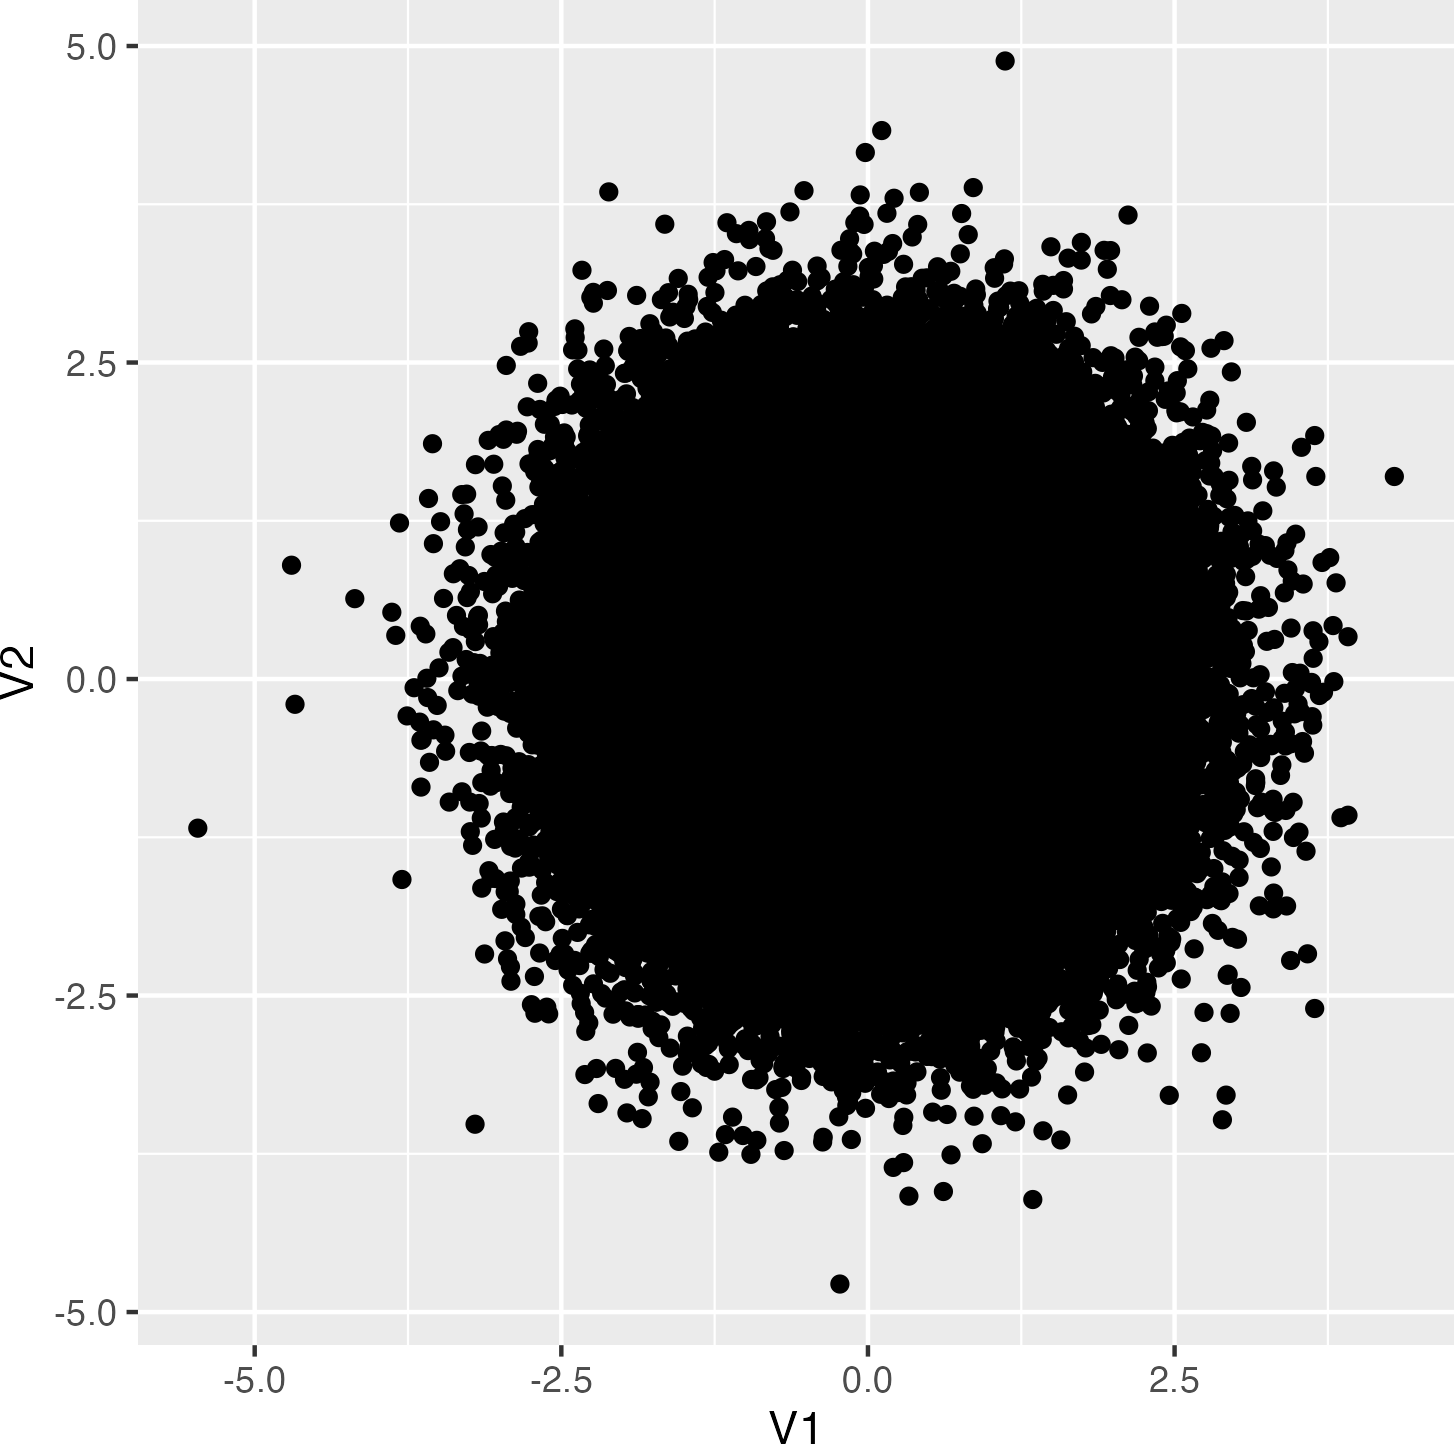
\includegraphics[keepaspectratio]{chapter07_files/figure-pdf/ggR-1.png}}

数値的にも確認しておこう。

\begin{Shaded}
\begin{Highlighting}[]
\FunctionTok{cor}\NormalTok{(X) }\SpecialCharTok{\%\textgreater{}\%} \FunctionTok{round}\NormalTok{(}\DecValTok{5}\NormalTok{)}
\end{Highlighting}
\end{Shaded}

\begin{verbatim}
     [,1] [,2]
[1,]    1    0
[2,]    0    1
\end{verbatim}

つくられた乱数が無相関であることが確認できた。さてこれが母集団であったとして,ここからたとえば\texttt{n\ =\ 20}のサンプルをとったとする。この時の相関はどうなるだろうか。
Rで計算してみよう。\texttt{sample}関数をつかって抜き出す行を決めて,該当する行だけ\texttt{s1}オブジェクトに代入する。その上で相関係数を計算してみよう。

\begin{Shaded}
\begin{Highlighting}[]
\NormalTok{selected\_row }\OtherTok{\textless{}{-}} \FunctionTok{sample}\NormalTok{(}\DecValTok{1}\SpecialCharTok{:}\NormalTok{N, }\DecValTok{20}\NormalTok{)}
\FunctionTok{print}\NormalTok{(selected\_row)}
\end{Highlighting}
\end{Shaded}

\begin{verbatim}
 [1]  9647 80702 57543 93179 99032 82624 32672 53670 69698 42383 23801 69303
[13]  9816 61803 69464 23107 76958 44447    10 27292
\end{verbatim}

\begin{Shaded}
\begin{Highlighting}[]
\NormalTok{s1 }\OtherTok{\textless{}{-}}\NormalTok{ X[selected\_row, ]}
\FunctionTok{cor}\NormalTok{(s1)}
\end{Highlighting}
\end{Shaded}

\begin{verbatim}
          [,1]      [,2]
[1,] 1.0000000 0.1431698
[2,] 0.1431698 1.0000000
\end{verbatim}

今回の相関係数は0.1431698となった。母集団の相関係数が0であっても,適当に抜き出した20点が相関係数を持ってしまう(0でない)ことはあり得ることなのである。問題は,これがどの程度あり得ることなのか,である。いいかえると,研究者が\(n=20\)のサンプルをとって相関を得た時,それが\(r = 0.14\)であったとしても,母相関\(\rho = 0.0\)からのサンプルである可能性がどれぐらいあるか,ということである。

\section{標本相関係数の分布と検定}\label{ux6a19ux672cux76f8ux95a2ux4fc2ux6570ux306eux5206ux5e03ux3068ux691cux5b9a}

標本相関係数は確率変数なので,毎回標本を取る度に値が変わるし,どの実現値がどの程度出現するかは標本分布で表現できる。
ではどのような標本分布に従うのだろうか。先ほどのサンプリングを繰り返して,乱数によって近似してみよう\footnote{このような二度手間を取らず,\texttt{mvrnorm}からサンプルサイズ20の乱数を反復生成しても良い。母集団を具体的なものとしてイメージするために,母相関が\texttt{0}の母集団からサンプリングを繰り返す方法をとった。}。

\begin{Shaded}
\begin{Highlighting}[]
\NormalTok{iter }\OtherTok{\textless{}{-}} \DecValTok{10000}
\NormalTok{samples }\OtherTok{\textless{}{-}} \FunctionTok{c}\NormalTok{()}
\ControlFlowTok{for}\NormalTok{ (i }\ControlFlowTok{in} \DecValTok{1}\SpecialCharTok{:}\NormalTok{iter) \{}
\NormalTok{  selected\_row }\OtherTok{\textless{}{-}} \FunctionTok{sample}\NormalTok{(}\DecValTok{1}\SpecialCharTok{:}\NormalTok{N, }\DecValTok{20}\NormalTok{)}
\NormalTok{  s\_i }\OtherTok{\textless{}{-}}\NormalTok{ X[selected\_row, ]}
\NormalTok{  cor\_i }\OtherTok{\textless{}{-}} \FunctionTok{cor}\NormalTok{(s\_i)[}\DecValTok{1}\NormalTok{, }\DecValTok{2}\NormalTok{]}
\NormalTok{  samples }\OtherTok{\textless{}{-}} \FunctionTok{c}\NormalTok{(samples, cor\_i)}
\NormalTok{\}}
\NormalTok{df }\OtherTok{\textless{}{-}} \FunctionTok{data.frame}\NormalTok{(}\AttributeTok{R =}\NormalTok{ samples)}
\CommentTok{\# ヒストグラムの描画}
\NormalTok{g }\OtherTok{\textless{}{-}}\NormalTok{ df }\SpecialCharTok{\%\textgreater{}\%}
  \FunctionTok{ggplot}\NormalTok{(}\FunctionTok{aes}\NormalTok{(}\AttributeTok{x =}\NormalTok{ R)) }\SpecialCharTok{+}
  \FunctionTok{geom\_histogram}\NormalTok{(}\AttributeTok{binwidth =} \FloatTok{0.01}\NormalTok{)}
\FunctionTok{print}\NormalTok{(g)}
\end{Highlighting}
\end{Shaded}

\pandocbounded{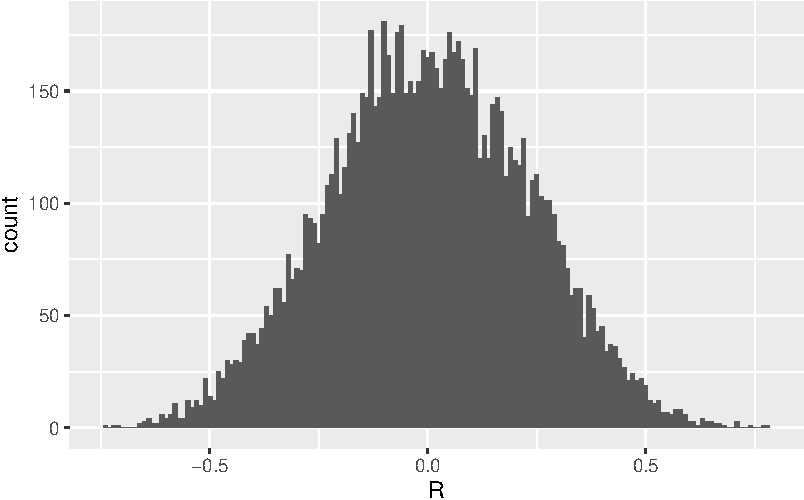
\includegraphics[keepaspectratio]{chapter07_files/figure-pdf/sampleDist-1.pdf}}

ヒストグラムを見ると,サンプルサイズが20の場合,母相関係数\(\rho = 0.0\)であっても\(r = 0.3\)や\(r=0.4\)程度の標本相関が出現することはある程度みられることである。

また,標本分布は左右対称の何らかの理論分布に従っていそうだ。数理統計学の知見から,相関係数の場合,標本相関係数を次の式によって変換することで,自由度が\(n-2\)の\(t\)分布に従うことが知られている。

\[ t = \frac{r\sqrt{n-2}}{\sqrt{1-r^2}} \]

\begin{Shaded}
\begin{Highlighting}[]
\NormalTok{df }\SpecialCharTok{\%\textgreater{}\%}
  \FunctionTok{mutate}\NormalTok{(}\AttributeTok{T =}\NormalTok{ R }\SpecialCharTok{*} \FunctionTok{sqrt}\NormalTok{(}\DecValTok{18}\NormalTok{) }\SpecialCharTok{/} \FunctionTok{sqrt}\NormalTok{(}\DecValTok{1} \SpecialCharTok{{-}}\NormalTok{ R}\SpecialCharTok{\^{}}\DecValTok{2}\NormalTok{)) }\SpecialCharTok{\%\textgreater{}\%}
  \FunctionTok{ggplot}\NormalTok{(}\FunctionTok{aes}\NormalTok{(}\AttributeTok{x =}\NormalTok{ T)) }\SpecialCharTok{+}
  \FunctionTok{geom\_histogram}\NormalTok{(}\FunctionTok{aes}\NormalTok{(}\AttributeTok{y =} \FunctionTok{after\_stat}\NormalTok{(density)), }\AttributeTok{binwidth =} \FloatTok{0.1}\NormalTok{) }\SpecialCharTok{+}
  \CommentTok{\# 自由度18のt分布の確率密度関数を追加}
  \FunctionTok{stat\_function}\NormalTok{(}\AttributeTok{fun =}\NormalTok{ dt, }\AttributeTok{args =} \FunctionTok{list}\NormalTok{(}\AttributeTok{df =} \DecValTok{18}\NormalTok{), }\AttributeTok{color =} \StringTok{"red"}\NormalTok{, }\AttributeTok{linewidth =} \DecValTok{2}\NormalTok{) }\SpecialCharTok{+}
  \CommentTok{\# Y軸のラベルを変更}
  \FunctionTok{ylab}\NormalTok{(}\StringTok{"Density"}\NormalTok{)}
\end{Highlighting}
\end{Shaded}

\pandocbounded{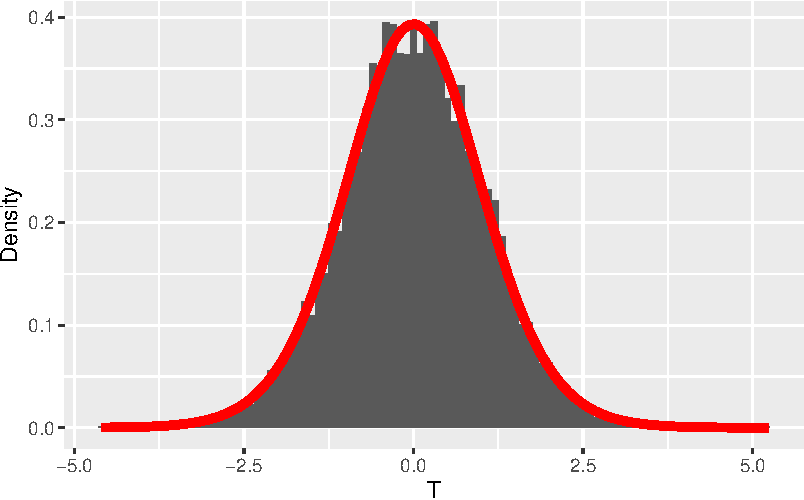
\includegraphics[keepaspectratio]{chapter07_files/figure-pdf/tprob-1.pdf}}

これを利用して相関係数の検定が行われる。以下,サンプルサイズ20で標本相関係数が\(r=0.5\)だったとして,手順に沿って解説する。

\begin{enumerate}
\def\labelenumi{\arabic{enumi}.}
\tightlist
\item
  帰無仮説は母相関\(\rho = 0.0\)とする。対立仮説は\(\rho \neq 0.0\)である。
\item
  検定統計量は相関係数\(r\)を変換した\(t\)とする。
\item
  判定基準として,\(\alpha = 0.05\)とする。すなわち,母相関が0であるという仮説を棄却して間違える確率を5\%以下に制御したい。
\item
  検定統計量を計算する。\(n=20,r=0.5\) より,
  \[t = \frac{0.5\times(\sqrt{18})}{\sqrt{1-0.5^2}} = 2.449\]
\item
  標本相関係数の\textbf{絶対値が}0.5を\textbf{超える}確率は,\(t\)分布の理論値から,次のように計算できる。あるいは,\(t\)分布の両端5\%を切り出す\textbf{臨界値}
  を次のように計算できる。
\end{enumerate}

\begin{Shaded}
\begin{Highlighting}[]
\NormalTok{(}\DecValTok{1} \SpecialCharTok{{-}} \FunctionTok{pt}\NormalTok{(}\FloatTok{0.5} \SpecialCharTok{*} \FunctionTok{sqrt}\NormalTok{(}\DecValTok{18}\NormalTok{) }\SpecialCharTok{/} \FunctionTok{sqrt}\NormalTok{(}\DecValTok{1} \SpecialCharTok{{-}} \FloatTok{0.5}\SpecialCharTok{\^{}}\DecValTok{2}\NormalTok{), }\AttributeTok{df =} \DecValTok{18}\NormalTok{)) }\SpecialCharTok{*} \DecValTok{2}
\end{Highlighting}
\end{Shaded}

\begin{verbatim}
[1] 0.02476956
\end{verbatim}

\begin{Shaded}
\begin{Highlighting}[]
\FunctionTok{qt}\NormalTok{(}\FloatTok{0.975}\NormalTok{, }\AttributeTok{df =} \DecValTok{18}\NormalTok{)}
\end{Highlighting}
\end{Shaded}

\begin{verbatim}
[1] 2.100922
\end{verbatim}

ここで注意してほしい点は,今回の検定の目的が「母相関が0であるという帰無仮説を棄却できるかどうか」であり,相関係数の符号については関心がなく絶対値で考える点である。\texttt{pt}関数は,ある確率点までの累積面積であるから,1から引くことでその確率点以上の値がでる確率が示される。\(t\)分布は左右対称の分布なので,これを2倍した値が絶対値で考えた時の出現確率である。これが5\%よりも小さければ,有意であると判断できる。今回は,統計的に有意であるといって良い。

なお,表現上の細かい注意点になるが,この確率は今回の実現値「以上」のより極端な値が出る確率であり,この実現値が出る確率という言い方はしない。確率は面積であり,点に対する面積はないからである。

\texttt{qt}関数で示されるのは確率点なので,これ以上の値を今回の実現値が出していたら,統計的に有意であると判断できる。今回の実現値から算出した値は\(t(18)=2.449\)であり,臨界値の\(2.100\)よりも大きな値なので,有意であると判断できる。

\section{2種類の検定のエラー確率}\label{ux7a2eux985eux306eux691cux5b9aux306eux30a8ux30e9ux30fcux78baux7387}

上では丁寧に計算過程をみてきたが,実践場面ではサンプルはひとつであり,標本統計量もひとつ算出されるだけである。自分の大切なデータであるから,標本分布から得られた特定のケースにすぎないことが直感的にわかりにくいかもしれない。

相関係数の検定をするときは,Rの関数\texttt{cor.test}を使って次のように行う。ここでは\texttt{mvrnorm}関数を使って,相関係数0.5の仮想データを作っている。

\begin{Shaded}
\begin{Highlighting}[]
\FunctionTok{set.seed}\NormalTok{(}\DecValTok{17}\NormalTok{)}
\NormalTok{n }\OtherTok{\textless{}{-}} \DecValTok{20}
\NormalTok{sampleData }\OtherTok{\textless{}{-}} \FunctionTok{mvrnorm}\NormalTok{(n,}
  \AttributeTok{mu =} \FunctionTok{c}\NormalTok{(}\DecValTok{0}\NormalTok{, }\DecValTok{0}\NormalTok{),}
  \AttributeTok{Sigma =} \FunctionTok{matrix}\NormalTok{(}\FunctionTok{c}\NormalTok{(}\DecValTok{1}\NormalTok{, }\FloatTok{0.5}\NormalTok{, }\FloatTok{0.5}\NormalTok{, }\DecValTok{1}\NormalTok{), }\AttributeTok{ncol =} \DecValTok{2}\NormalTok{),}
  \AttributeTok{empirical =} \ConstantTok{TRUE}
\NormalTok{)}
\FunctionTok{cor.test}\NormalTok{(sampleData[, }\DecValTok{1}\NormalTok{], sampleData[, }\DecValTok{2}\NormalTok{])}
\end{Highlighting}
\end{Shaded}

\begin{verbatim}

    Pearson's product-moment correlation

data:  sampleData[, 1] and sampleData[, 2]
t = 2.4495, df = 18, p-value = 0.02477
alternative hypothesis: true correlation is not equal to 0
95 percent confidence interval:
 0.07381057 0.77176071
sample estimates:
cor 
0.5 
\end{verbatim}

結果として示されている,tの値や自由度,\(p\)値が先ほど示した例と対応していることを確認できる。さらに,相関係数の信頼区間や標本相関係数そのものも示されている。この信頼区間が0を跨いでいないことからも,帰無仮説が棄却されることが見て取れるだろう。

われわれは既に,母相関が0のデータセットの一部を取り出すと,その相関係数が0ではなく0.5のような数字になることも知っている。もちろん母相関が0であれば標本相関も0近い値が出やすいとしても,である。つまり標本から得られた値をあまり大事に考えすぎない方が良い(もちろん一般化を念頭においている時は,である)。
また,帰無仮説は「母相関が0である」なので,これが\textbf{棄却}されたとしても「母相関が0であるとは言えない」のに過ぎない。ここから,母相関も\(r=0.5\)付近にあるはずだとか,\(p\)値が2.4\%なので5\%よりもずいぶん低いのは証拠の重要さを物語っているのだ,と論じるのは適切ではない。母相関が0という仮想的な状況のもとでの話であって,母相関が実際にどの程度なのかを検討しているわけではない。この点が誤解されやすいので特に注意してほしい。

ここに来るとタイプ1エラー,タイプ2エラーがより具体的に理解できるようになってきたではないだろうか。タイプ1エラーはこの帰無仮説が正しい時に,標本相関から計算した統計量で判断する確率であるから,上の手続きで見たことそのものである。

別の角度で見てみよう。\texttt{cor.test}をつかうと標本統計量の信頼区間が算出できる。この信頼区間が母相関--ここでは帰無仮説である\(\rho =0\)を「正しく」含んでいる割合を見てみよう。
\texttt{cor.test}関数が返すオブジェクトには,\texttt{conf.int}という名前のものがあり,デフォルトではここで95\%の信頼区間が含まれている。
シミュレーションに先立って,結果を格納する2列のデータフレームを作っておき,シミュレーション後に\texttt{ifelse}関数で母相関が含まれているかどうかの判定をした。

\begin{Shaded}
\begin{Highlighting}[]
\FunctionTok{set.seed}\NormalTok{(}\DecValTok{42}\NormalTok{)}
\NormalTok{iter }\OtherTok{\textless{}{-}} \DecValTok{10000}
\NormalTok{intervals }\OtherTok{\textless{}{-}} \FunctionTok{data.frame}\NormalTok{(}\FunctionTok{matrix}\NormalTok{(}\ConstantTok{NA}\NormalTok{, }\AttributeTok{nrow =}\NormalTok{ iter, }\AttributeTok{ncol =} \DecValTok{2}\NormalTok{))}
\FunctionTok{names}\NormalTok{(intervals) }\OtherTok{\textless{}{-}} \FunctionTok{c}\NormalTok{(}\StringTok{"Lower"}\NormalTok{, }\StringTok{"Upper"}\NormalTok{)}
\ControlFlowTok{for}\NormalTok{ (i }\ControlFlowTok{in} \DecValTok{1}\SpecialCharTok{:}\NormalTok{iter) \{}
\NormalTok{  selected\_row }\OtherTok{\textless{}{-}} \FunctionTok{sample}\NormalTok{(}\DecValTok{1}\SpecialCharTok{:}\NormalTok{N, }\DecValTok{20}\NormalTok{)}
\NormalTok{  s\_i }\OtherTok{\textless{}{-}}\NormalTok{ X[selected\_row, ]}
\NormalTok{  cor\_i }\OtherTok{\textless{}{-}} \FunctionTok{cor.test}\NormalTok{(s\_i[, }\DecValTok{1}\NormalTok{], s\_i[, }\DecValTok{2}\NormalTok{])}
\NormalTok{  intervals[i, ] }\OtherTok{\textless{}{-}}\NormalTok{ cor\_i}\SpecialCharTok{$}\NormalTok{conf.int[}\DecValTok{1}\SpecialCharTok{:}\DecValTok{2}\NormalTok{]}
\NormalTok{\}}
\CommentTok{\#}
\NormalTok{df }\OtherTok{\textless{}{-}}\NormalTok{ intervals }\SpecialCharTok{\%\textgreater{}\%}
  \FunctionTok{mutate}\NormalTok{(}\AttributeTok{FLG =} \FunctionTok{ifelse}\NormalTok{(Lower }\SpecialCharTok{\textless{}=} \DecValTok{0} \SpecialCharTok{\&}\NormalTok{ Upper }\SpecialCharTok{\textgreater{}=} \DecValTok{0}\NormalTok{, }\DecValTok{1}\NormalTok{, }\DecValTok{0}\NormalTok{)) }\SpecialCharTok{\%\textgreater{}\%}
  \FunctionTok{summarise}\NormalTok{(}\AttributeTok{type1error =} \FunctionTok{mean}\NormalTok{(FLG)) }\SpecialCharTok{\%\textgreater{}\%}
  \FunctionTok{print}\NormalTok{()}
\end{Highlighting}
\end{Shaded}

\begin{verbatim}
  type1error
1       0.95
\end{verbatim}

今回の例では,95\%の割合で正しく判断できていた。言い換えると,エラーが生じる割合は5\%だったので,タイプ1エラー確率を5\%以下にするという目的はしっかり達成できていたことが確認できた。

同様に,タイプ2エラーは,帰無仮説が正しくないときに帰無仮説を採択する確率だから,シミュレーションするなら次のようになる。まず母相関が0でない状況を作り出そう。今回は母相関が0.5であるとして,母集団分布を描いてみよう。

\begin{Shaded}
\begin{Highlighting}[]
\FunctionTok{set.seed}\NormalTok{(}\DecValTok{12345}\NormalTok{)}
\NormalTok{N }\OtherTok{\textless{}{-}} \DecValTok{100000}
\NormalTok{X }\OtherTok{\textless{}{-}} \FunctionTok{mvrnorm}\NormalTok{(N,}
  \AttributeTok{mu =} \FunctionTok{c}\NormalTok{(}\DecValTok{0}\NormalTok{, }\DecValTok{0}\NormalTok{),}
  \AttributeTok{Sigma =} \FunctionTok{matrix}\NormalTok{(}\FunctionTok{c}\NormalTok{(}\DecValTok{1}\NormalTok{, }\FloatTok{0.5}\NormalTok{, }\FloatTok{0.5}\NormalTok{, }\DecValTok{1}\NormalTok{), }\AttributeTok{ncol =} \DecValTok{2}\NormalTok{),}
  \AttributeTok{empirical =} \ConstantTok{TRUE}
\NormalTok{)}

\NormalTok{X }\SpecialCharTok{\%\textgreater{}\%}
  \FunctionTok{as.data.frame}\NormalTok{() }\SpecialCharTok{\%\textgreater{}\%}
  \FunctionTok{ggplot}\NormalTok{(}\FunctionTok{aes}\NormalTok{(}\AttributeTok{x =}\NormalTok{ V1, }\AttributeTok{y =}\NormalTok{ V2)) }\SpecialCharTok{+}
  \FunctionTok{geom\_point}\NormalTok{()}
\end{Highlighting}
\end{Shaded}

\pandocbounded{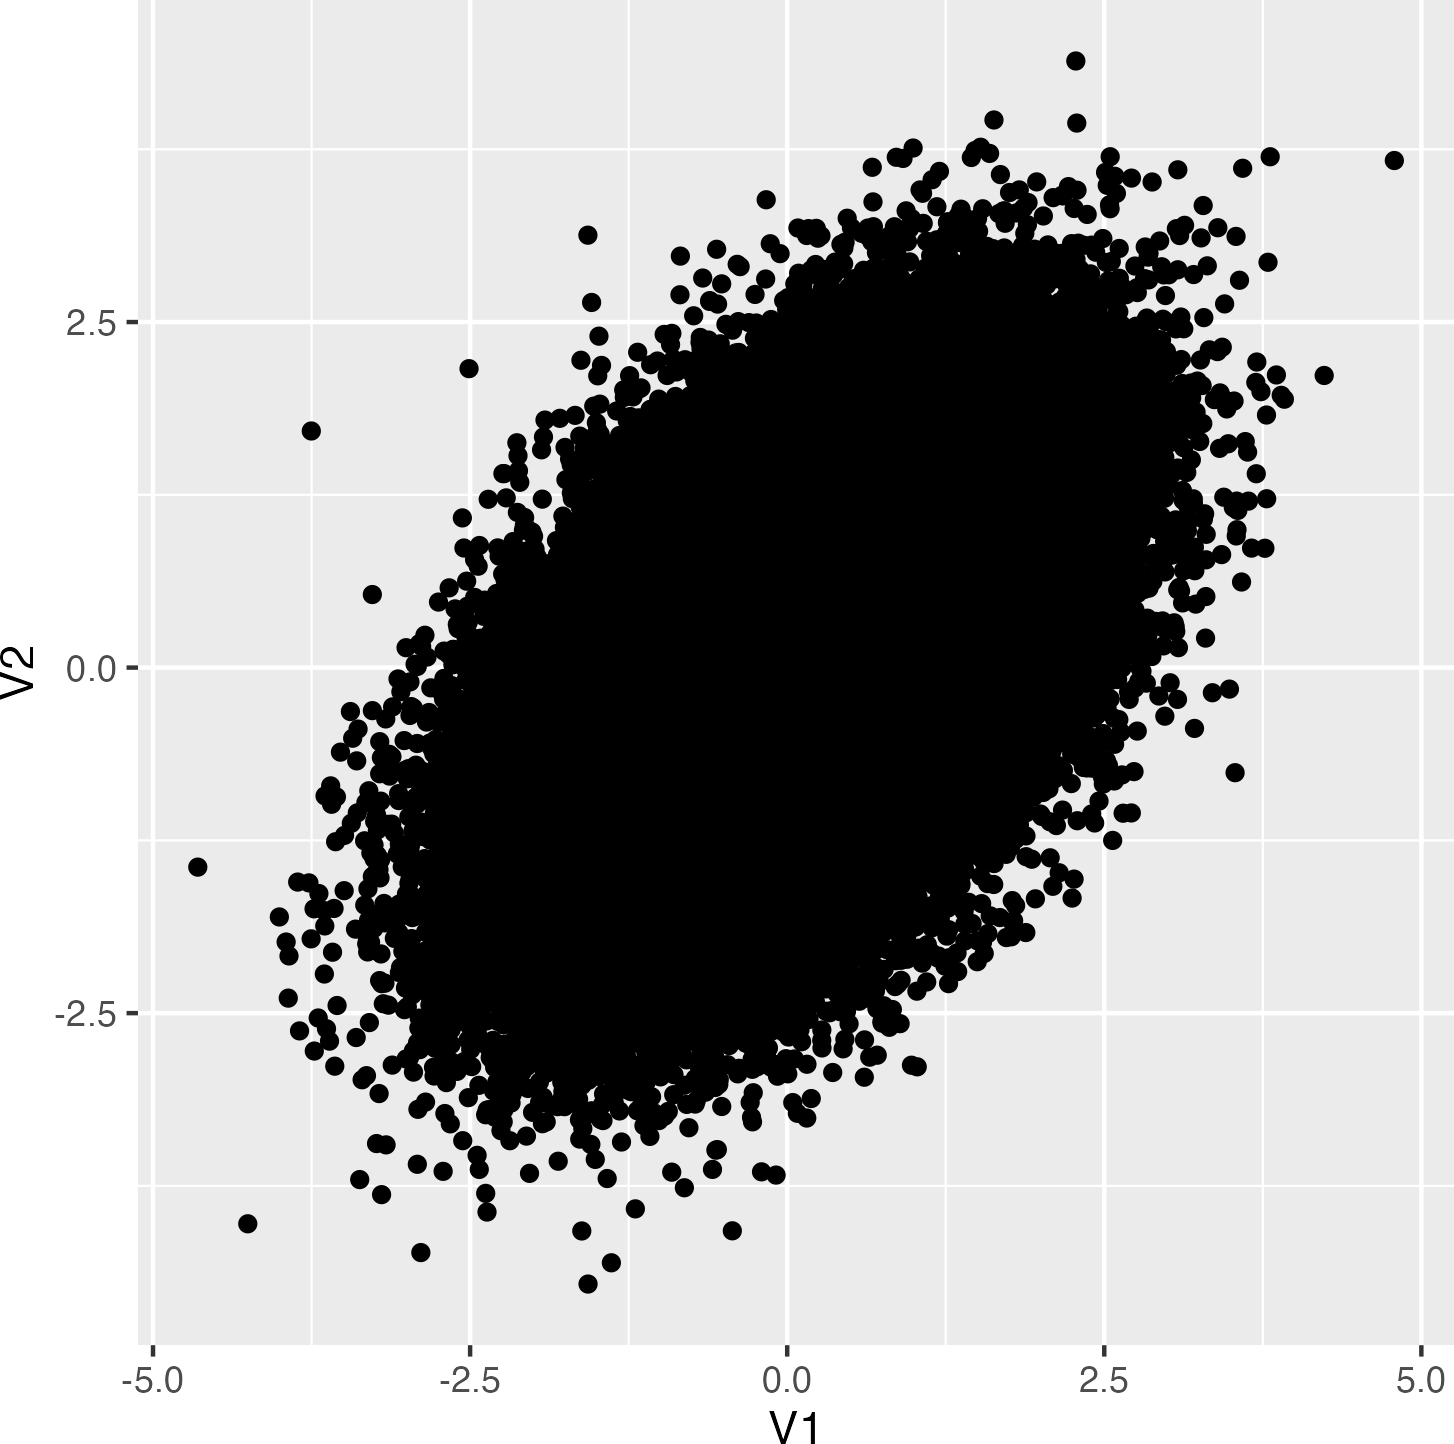
\includegraphics[keepaspectratio]{chapter07_files/figure-pdf/gg0.5-1.png}}

今度は,ここからサンプルサイズ20のデータセットを取り出し,検定することにしよう。検定の結果,有意になれば\texttt{1},ならなければ\texttt{0}というオブジェクトを作って,判定の正しさを考えてみることにする。

\begin{Shaded}
\begin{Highlighting}[]
\NormalTok{iter }\OtherTok{\textless{}{-}} \DecValTok{10000}
\NormalTok{judges }\OtherTok{\textless{}{-}} \FunctionTok{c}\NormalTok{()}
\ControlFlowTok{for}\NormalTok{ (i }\ControlFlowTok{in} \DecValTok{1}\SpecialCharTok{:}\NormalTok{iter) \{}
\NormalTok{  selected\_row }\OtherTok{\textless{}{-}} \FunctionTok{sample}\NormalTok{(}\DecValTok{1}\SpecialCharTok{:}\NormalTok{N, }\DecValTok{20}\NormalTok{)}
\NormalTok{  s\_i }\OtherTok{\textless{}{-}}\NormalTok{ X[selected\_row, ]}
\NormalTok{  cor\_i }\OtherTok{\textless{}{-}} \FunctionTok{cor.test}\NormalTok{(s\_i[, }\DecValTok{1}\NormalTok{], s\_i[, }\DecValTok{2}\NormalTok{])}
\NormalTok{  judges }\OtherTok{\textless{}{-}} \FunctionTok{c}\NormalTok{(judges, cor\_i}\SpecialCharTok{$}\NormalTok{p.value)}
\NormalTok{\}}
\NormalTok{df }\OtherTok{\textless{}{-}} \FunctionTok{data.frame}\NormalTok{(}\AttributeTok{p =}\NormalTok{ judges) }\SpecialCharTok{\%\textgreater{}\%}
  \FunctionTok{mutate}\NormalTok{(}\AttributeTok{FLG =} \FunctionTok{ifelse}\NormalTok{(p }\SpecialCharTok{\textless{}=} \FloatTok{0.05}\NormalTok{, }\DecValTok{1}\NormalTok{, }\DecValTok{0}\NormalTok{)) }\SpecialCharTok{\%\textgreater{}\%}
  \FunctionTok{summarise}\NormalTok{(}
    \AttributeTok{sig =} \FunctionTok{sum}\NormalTok{(FLG }\SpecialCharTok{==} \DecValTok{1}\NormalTok{),}
    \AttributeTok{non.sig =} \FunctionTok{sum}\NormalTok{(FLG }\SpecialCharTok{==} \DecValTok{0}\NormalTok{),}
    \AttributeTok{type2error =}\NormalTok{ non.sig }\SpecialCharTok{/}\NormalTok{ iter}
\NormalTok{  ) }\SpecialCharTok{\%\textgreater{}\%}
  \FunctionTok{print}\NormalTok{()}
\end{Highlighting}
\end{Shaded}

\begin{verbatim}
   sig non.sig type2error
1 6442    3558     0.3558
\end{verbatim}

今回は母相関が0.5であり,帰無仮説は棄却されて然るべきなのだが,有意でないと判断された割合が35.58\%あったことになる。心理学の研究などでは,この確率\(\beta\)が0.2未満,逆にいうと検出が0.8以上あることが望ましいとされているので,今回のこの事例では十分な件出力がなかった,と言えるだろう。

もちろん実際には,母相関がどれぐらいなのかわからない。\(0.3\)なのかもしれないし,\(-0.5\)であるかもしれない。つまりタイプ2エラーは研究者が制御できるところではなく,せいぜい大きな相関が見込めそうな変数について標本を取ろうと心がけるだけである。

タイプ1,2エラーの確率は,サンプルサイズや効果量(ここでは母相関の大きさ)の関数である。サンプルサイズは研究者が決定することができるので,効果を見積もり,制御したいエラー確率の基準を決めて,合理的にサンプルサイズを決めるべきである。

\section{課題}\label{ux8ab2ux984c-5}

\begin{enumerate}
\def\labelenumi{\arabic{enumi}.}
\tightlist
\item
  母相関が0の母集団から,サンプルサイズ10の標本を取り出して標本相関を見た時の標本分布を,乱数のヒストグラムで近似してみましょう。
\item
  同じく,サンプルサイズ50の標本を取り出して標本相関を見た時の標本分布を,乱数のヒストグラムで近似してみましょう。サンプルサイズが20や10の時と比べてどういう違いがあるでしょうか。
\item
  サンプルサイズ50の標本相関が\(r=-0.3\)のとき,統計的に有意と言えるでしょうか。\texttt{cor.test}
  をつかって検定し,検定結果と判断結果を記述してください。
\item
  標本相関が\(r=-0.3\)だとします。サンプルサイズが10,20,50,1000のとき,統計的に有意と言えるでしょうか。\texttt{cor.test}を使って検定し,検定結果を一覧にしてみましょう。ここから何がわかるでしょうか。
\item
  母相関が\(\rho = -0.3\)だったとします。サンプルサイズ20のとき,どの程度の検出力があると見込めるでしょうか。シミュレーションで近似してください。
\end{enumerate}

\bookmarksetup{startatroot}

\chapter{平均値差の検定}\label{ux5e73ux5747ux5024ux5deeux306eux691cux5b9a}

平均値差の検定は,実験計画の結論を出すために用いられる手段である。無作為割り当てによって個人差や背景要因が相殺され,平均的な因果効果を検証することができるからである。
その結果を一般化するためには,やはり推測統計学の知見が必要であり,サンプルサイズやタイプ1,2エラーが関わってくることに変わりはない。

\section{一標本検定}\label{ux4e00ux6a19ux672cux691cux5b9a}

まず配置標本検定の例から始める。母平均がわかっている,あるいは理論的に仮定される特定の値に対して,標本平均が統計的に有意に異なっていると言って良いかどうかの判断をするときに用いる。
たとえば7件法のデータを取ったときに,ある項目の平均が中点4より有意に離れていると言って良いかどうか,といった判定をするときに用いる。かりに,サンプルサイズ10で7件法のデータが得られたとしよう。ここでは平均4,SD1の正規乱数を10件生成することで表現する。実際にはこの値を,人に対する尺度カテゴリへの反応として得ているはずである。

\begin{Shaded}
\begin{Highlighting}[]
\NormalTok{pacman}\SpecialCharTok{::}\FunctionTok{p\_load}\NormalTok{(tidyverse)}
\FunctionTok{set.seed}\NormalTok{(}\DecValTok{17}\NormalTok{)}
\NormalTok{n }\OtherTok{\textless{}{-}} \DecValTok{10}
\NormalTok{mu }\OtherTok{\textless{}{-}} \DecValTok{4}
\NormalTok{X }\OtherTok{\textless{}{-}} \FunctionTok{rnorm}\NormalTok{(n, }\AttributeTok{mean =}\NormalTok{ mu, }\AttributeTok{sd =} \DecValTok{1}\NormalTok{)}
\FunctionTok{print}\NormalTok{(X)}
\end{Highlighting}
\end{Shaded}

\begin{verbatim}
 [1] 2.984991 3.920363 3.767013 3.182732 4.772091 3.834388 4.972874 5.716534
 [9] 4.255237 4.366581
\end{verbatim}

今回,標本平均は4.177であり,これより極端な値が\(\mu = 4\)の母集団から得られるかどうかを検定する。帰無仮説検定の手順にそって進めていくと,以下のようになる。

\begin{enumerate}
\def\labelenumi{\arabic{enumi}.}
\tightlist
\item
  帰無仮説は母平均が理論的な値(ここでは尺度の中点4)であること,すなわち\(\mu =4\)であり,対立仮説は\(\mu \neq 4\)
  である。
\item
  検定統計量は,正規母集団から得られる標本平均が従う標本分布であり,母分散が未知の場合の区間推定に用いたT統計量になる。
\item
  判断基準は心理学の慣例に沿って5\%とする。
\end{enumerate}

このあと,検定統計量の計算と判定である。これをRは\texttt{t.test}関数で一気に処理できる。

\begin{Shaded}
\begin{Highlighting}[]
\NormalTok{result }\OtherTok{\textless{}{-}} \FunctionTok{t.test}\NormalTok{(X, }\AttributeTok{mu =}\NormalTok{ mu)}
\FunctionTok{print}\NormalTok{(result)}
\end{Highlighting}
\end{Shaded}

\begin{verbatim}

    One Sample t-test

data:  X
t = 0.6776, df = 9, p-value = 0.5151
alternative hypothesis: true mean is not equal to 4
95 percent confidence interval:
 3.585430 4.769131
sample estimates:
mean of x 
 4.177281 
\end{verbatim}

結果として,今回の検定統計量の実現値は0.678であり,自由度9のt分布からこれ以上の値が出てくる確率は,0.515であることがわかる。これは5\%水準と見比べてより大きいので,レアケースではないと判断できる。つまり,母平均4の正規母集団から,4.177の標本平均が得られることはそれほど珍しいものではなく,統計的に有意に異なっていると判断するには及ばない,ということである。

レポートなどに記載するときは,これら実現値やp値を踏まえて「\(t(9)=0.66776,p=0.5151 ,n.s.\)」などとする。ここでn.s.はnot
significantの略である。

さてこの例では,母平均4の正規乱数を生成し,その平均が4と異なるとはいえない,と結論づけた。これは一見,当たり前のことのようであり,無意味な行為におもえるかもしれない。しかし次の例を見てみよう。

\begin{Shaded}
\begin{Highlighting}[]
\NormalTok{n }\OtherTok{\textless{}{-}} \DecValTok{3}
\NormalTok{mu }\OtherTok{\textless{}{-}} \DecValTok{4}
\NormalTok{X }\OtherTok{\textless{}{-}} \FunctionTok{rnorm}\NormalTok{(n, }\AttributeTok{mean =}\NormalTok{ mu, }\AttributeTok{sd =} \DecValTok{1}\NormalTok{)}
\FunctionTok{mean}\NormalTok{(X) }\SpecialCharTok{\%\textgreater{}\%}
  \FunctionTok{round}\NormalTok{(}\DecValTok{3}\NormalTok{) }\SpecialCharTok{\%\textgreater{}\%}
  \FunctionTok{print}\NormalTok{()}
\end{Highlighting}
\end{Shaded}

\begin{verbatim}
[1] 5.04
\end{verbatim}

\begin{Shaded}
\begin{Highlighting}[]
\NormalTok{result }\OtherTok{\textless{}{-}} \FunctionTok{t.test}\NormalTok{(X, }\AttributeTok{mu =}\NormalTok{ mu)}
\FunctionTok{print}\NormalTok{(result)}
\end{Highlighting}
\end{Shaded}

\begin{verbatim}

    One Sample t-test

data:  X
t = 5.1723, df = 2, p-value = 0.03541
alternative hypothesis: true mean is not equal to 4
95 percent confidence interval:
 4.174825 5.904710
sample estimates:
mean of x 
 5.039768 
\end{verbatim}

ここではサンプルサイズ\(n=3\)であり,標本平均が5.04であった。このときt値は5\%臨界値を上回っており,「母平均4のところから得られる値にしては極端」であるから,統計的に有意に異なる,と判断することになる。乱数生成時は平均を確かに4に設定したが,母平均から取り出したごく一部が,そこから大きく離れてしまうことはあり得るのである。

\section{二標本検定}\label{ux4e8cux6a19ux672cux691cux5b9a}

続いて二標本の検定について考えよう。実験群と統制群のように,無作為割り当てをすることで平均因果効果をみる際に行われるのが,この検定である。帰無仮説は「群間差はない」であり,対立仮説はその否定である。また,正規母集団からの標本を仮定するので,検定統計量はここでもt分布に従う値になる。帰無仮説検定の手順に沿って,改めて確認しておこう。

\begin{enumerate}
\def\labelenumi{\arabic{enumi}.}
\tightlist
\item
  帰無仮説は「二群の母平均に差がない」である。二群の母平均をそれぞれ\(\mu_1,\mu_2\)とすると,帰無仮説は\(\mu_1 = \mu_2\),あるいは\(\mu_1 - \mu_2 = 0\)と表される。対立仮説は\(\mu_1 \neq \mu_2\)あるいは\(\mu_1-\mu_2 \neq 0\)である。
\item
  検定統計量は,正規母集団から得られる標本平均が従う標本分布であり,母分散が未知の場合の区間推定に用いたT統計量になる。
\item
  判断基準は心理学の慣例に沿って5\%とする。
\end{enumerate}

これを検証するために,サンプルデータを乱数で生成しよう。
まず,各群のサンプルサイズを\texttt{n1,n2}とする。ここでは話を簡単にするため,サンプルサイズは両群ともに\texttt{10}とした。つぎに両群の母平均だが,群1の母平均を\(\mu_1\),群2の母平均を\(\mu_2 = \mu_1 + \delta\)で表現した。この\(\delta\)は差分であり,これが\(\delta=0\)であれば母平均が等しいこと,\(\delta \neq 0\)であれば母平均が異なることになる。最後に両群の母SDを設定した。

ここでの検定は,この差分\(d\)が母平均0の母集団から得られたと判断して良いかどうか,という形で行われる。検定統計量\(T\)は,次式で算出されるものである。

\[ T = \frac{d - \mu_0}{\sqrt{U^2_p/\frac{n_1n_2}{n_1+n_2}}}\]

ここで\(d\)は二群の標本平均の差であり,\(U^2_p\)はプールされた不偏分散と呼ばれ,二群を合わせて計算された全体の母分散推定量である。各群の標本分散をそれぞれ\(S^2_1, S^2_2\)とすると,次式で算出される。

\[ U^2_p = \frac{n_1S^2_1+ n_2S^2_2}{n_1 + n_2 -2} \]

これらの式はつまり,サンプルサイズの違いを考慮するため,一旦両群の標本分散に各サンプルサイズを掛け合わせ,プールした全体のサンプルサイズから各々\(-1\)をすることで全体として不偏分散にしている。

これを踏まえて,具体的な数字で見ていこう。
その上で乱数でデータを生成し,その標本平均を確認した上で,\texttt{t.test}関数によって検定を行っている。

\begin{Shaded}
\begin{Highlighting}[]
\NormalTok{n1 }\OtherTok{\textless{}{-}} \DecValTok{10}
\NormalTok{n2 }\OtherTok{\textless{}{-}} \DecValTok{10}
\NormalTok{mu1 }\OtherTok{\textless{}{-}} \DecValTok{4}
\NormalTok{sigma }\OtherTok{\textless{}{-}} \DecValTok{1}
\NormalTok{delta }\OtherTok{\textless{}{-}} \DecValTok{1}
\NormalTok{mu2 }\OtherTok{\textless{}{-}}\NormalTok{ mu1 }\SpecialCharTok{+}\NormalTok{ (sigma }\SpecialCharTok{*}\NormalTok{ delta)}

\FunctionTok{set.seed}\NormalTok{(}\DecValTok{42}\NormalTok{)}
\NormalTok{X1 }\OtherTok{\textless{}{-}} \FunctionTok{rnorm}\NormalTok{(n1, }\AttributeTok{mean =}\NormalTok{ mu1, }\AttributeTok{sd =}\NormalTok{ sigma)}
\NormalTok{X2 }\OtherTok{\textless{}{-}} \FunctionTok{rnorm}\NormalTok{(n2, }\AttributeTok{mean =}\NormalTok{ mu2, }\AttributeTok{sd =}\NormalTok{ sigma)}

\NormalTok{X1 }\SpecialCharTok{\%\textgreater{}\%}
  \FunctionTok{mean}\NormalTok{() }\SpecialCharTok{\%\textgreater{}\%}
  \FunctionTok{round}\NormalTok{(}\DecValTok{3}\NormalTok{) }\SpecialCharTok{\%\textgreater{}\%}
  \FunctionTok{print}\NormalTok{()}
\end{Highlighting}
\end{Shaded}

\begin{verbatim}
[1] 4.547
\end{verbatim}

\begin{Shaded}
\begin{Highlighting}[]
\NormalTok{X2 }\SpecialCharTok{\%\textgreater{}\%}
  \FunctionTok{mean}\NormalTok{() }\SpecialCharTok{\%\textgreater{}\%}
  \FunctionTok{round}\NormalTok{(}\DecValTok{3}\NormalTok{) }\SpecialCharTok{\%\textgreater{}\%}
  \FunctionTok{print}\NormalTok{()}
\end{Highlighting}
\end{Shaded}

\begin{verbatim}
[1] 4.837
\end{verbatim}

\begin{Shaded}
\begin{Highlighting}[]
\NormalTok{result }\OtherTok{\textless{}{-}} \FunctionTok{t.test}\NormalTok{(X1, X2, }\AttributeTok{var.equal =} \ConstantTok{TRUE}\NormalTok{)}
\FunctionTok{print}\NormalTok{(result)}
\end{Highlighting}
\end{Shaded}

\begin{verbatim}

    Two Sample t-test

data:  X1 and X2
t = -0.49924, df = 18, p-value = 0.6237
alternative hypothesis: true difference in means is not equal to 0
95 percent confidence interval:
 -1.506473  0.927980
sample estimates:
mean of x mean of y 
 4.547297  4.836543 
\end{verbatim}

今回の母平均は\(\mu_1 = 4, \mu_2 = 4+1\)にしているが,標本平均は4.547と4.837であり,標本上では大きな差が見られなかった。結果として,t値は0.4992369であり,自由度18のもとでのp値は0.6236593である。5\%水準を上回る値であるから,結論としては対立仮説を採択するには至らない,差があるとはいえない,である。

今回の設定では母平均に差があるはず(\(4 \neq 4 + 1\))なのだから,これは誤った判断で,タイプ2エラーが生じているケースということになる。研究実践場面では,母平均やその差については知り得ないのだから,このような判断ミスが生じていたかどうかは分かり得ないことに留意しよう。

なお,ここではわかりやすく2群であることを示すために\texttt{X1},\texttt{X2}と2つのオブジェクトを用意したが,実践的にはデータフレームの中で群わけを示す変数があり,\texttt{formula}の形で次のように書くことが多いだろう。

\begin{Shaded}
\begin{Highlighting}[]
\NormalTok{dataSet }\OtherTok{\textless{}{-}} \FunctionTok{data.frame}\NormalTok{(}\AttributeTok{group =} \FunctionTok{c}\NormalTok{(}\FunctionTok{rep}\NormalTok{(}\DecValTok{1}\NormalTok{, n1), }\FunctionTok{rep}\NormalTok{(}\DecValTok{2}\NormalTok{, n2)), }\AttributeTok{value =} \FunctionTok{c}\NormalTok{(X1, X2)) }\SpecialCharTok{\%\textgreater{}\%}
  \FunctionTok{mutate}\NormalTok{(}\AttributeTok{group =} \FunctionTok{as.factor}\NormalTok{(group))}
\FunctionTok{t.test}\NormalTok{(value }\SpecialCharTok{\textasciitilde{}}\NormalTok{ group, }\AttributeTok{data =}\NormalTok{ dataSet, }\AttributeTok{var.equal =} \ConstantTok{TRUE}\NormalTok{)}
\end{Highlighting}
\end{Shaded}

\begin{verbatim}

    Two Sample t-test

data:  value by group
t = -0.49924, df = 18, p-value = 0.6237
alternative hypothesis: true difference in means between group 1 and group 2 is not equal to 0
95 percent confidence interval:
 -1.506473  0.927980
sample estimates:
mean in group 1 mean in group 2 
       4.547297        4.836543 
\end{verbatim}

\section{二標本検定(ウェルチの補正)}\label{ux4e8cux6a19ux672cux691cux5b9aux30a6ux30a7ux30ebux30c1ux306eux88dcux6b63}

先ほどのt.test関数には,\texttt{var.equal\ =\ TRUE}というオプションが追加されていた。これは2群の分散が等しいと仮定した場合の検定になる。t検定は歴史的にこちらが先に登場しているが,2群の分散が等しいかどうかはいきなり前提できるものでもない。等分散性の検定は,Levene検定を行うのが一般的であり,R
においては,\texttt{car}パッケージや\texttt{lawstat}
パッケージが対応する関数を持っている。ここでは\texttt{car}パッケージの
\texttt{leveneTest}関数を用いる例を示す。

\begin{Shaded}
\begin{Highlighting}[]
\NormalTok{pacman}\SpecialCharTok{::}\FunctionTok{p\_load}\NormalTok{(car)}
\FunctionTok{leveneTest}\NormalTok{(value }\SpecialCharTok{\textasciitilde{}}\NormalTok{ group, }\AttributeTok{data =}\NormalTok{ dataSet, }\AttributeTok{center =}\NormalTok{ mean)}
\end{Highlighting}
\end{Shaded}

\begin{verbatim}
Levene's Test for Homogeneity of Variance (center = mean)
      Df F value Pr(>F)
group  1  2.9405 0.1035
      18               
\end{verbatim}

この結果を見ると,p値から明らかなように,2群の分散が等しいという帰無仮説が棄却\textbf{できなかった}ので,等しいと考えてt検定に進むことができる。もしこれが棄却されてしまったら,2群の分散が等しいという帰無仮説が成り立たないのだから,等分散性の仮定を外す必要がある。実行は簡単で,\texttt{var.equal}を\texttt{FALSE}にすれば良い。

\begin{Shaded}
\begin{Highlighting}[]
\NormalTok{result2 }\OtherTok{\textless{}{-}} \FunctionTok{t.test}\NormalTok{(value }\SpecialCharTok{\textasciitilde{}}\NormalTok{ group, }\AttributeTok{data =}\NormalTok{ dataSet, }\AttributeTok{var.equal =} \ConstantTok{FALSE}\NormalTok{)}
\FunctionTok{print}\NormalTok{(result2)}
\end{Highlighting}
\end{Shaded}

\begin{verbatim}

    Welch Two Sample t-test

data:  value by group
t = -0.49924, df = 13.421, p-value = 0.6257
alternative hypothesis: true difference in means between group 1 and group 2 is not equal to 0
95 percent confidence interval:
 -1.5369389  0.9584459
sample estimates:
mean in group 1 mean in group 2 
       4.547297        4.836543 
\end{verbatim}

よく見ると,タイトルがWelch Two Sample
t-testに変わっている。Welchの補正が入ったt検定という意味である。また自由度が実数(13.421)になっているが,このようにt分布の自由度を調整することで等分散性の仮定から逸脱した場合の補正となる。もちろん報告する際は「\(t(\)
13.421 \()=\) -0.499, \(p=\)
0.626」のように書くことになるから,自由度が実数であれば補正済みであると考えられるだろう。

しかし,分散が等しいという仮定は,等しくない場合の特殊な場合であるから,最初からWelchの補正がはいった検定だけで十分である。このような考え方から,Rにおける\texttt{t.test}
関数のデフォルトでは\texttt{var.equal\ =\ FALSE}となっており,特段の指定をしなければ等分散性の仮定をしない。こちらの方が検定を重ねることがないので,より望ましい。

\subsection{効果量の算出}\label{ux52b9ux679cux91cfux306eux7b97ux51fa}

今回の例は,仮想データとして\(\mu_1 = 4,\mu_2 = \mu_1 + \sigma d\)であり,明らかに\(\mu_1 \neq \mu_2\)なのだが,有意差を検出するには至らなかった。統計的な有意差はあくまでも「統計的な」観点からのものであり,我々が現実に検証したいのは本当に差があるかどうか,いわば「実質的な差」があるかどうかであるのだから,統計的な有意差を得ることを目的にするのははっきりと不適切な目標設定であると言えるだろう\footnote{たとえば物理学などのシーンでは,測定の精度が高く,単一の物理世界を対象にした検証を行うのだから,予測が真であるか偽であるかを確率的に考えるような必要はない。そのような世界における検証--あえて理論的な正しさが明確な世界,と表現するが--であれば,統計的な差があるかどうかの情報はあくまでも理論を支持するおまけ情報にすぎない。いわば統計的検定の結果を報告するのは,論文を書くためのレトリックである。例えば,ニュートンの運動法則やアインシュタインの相対性理論などの物理法則の検証では,測定誤差の範囲内で理論値と実験値が一致するかどうかが重要であり,統計的な有意性は二次的な情報に過ぎない。翻って,人間を対象にした小サンプルの科学である心理学は,統計的な判断に頼らざるを得ないという側面はあるだろう。しかしだからと言って,実質的な差が本質的であることを忘れてしまっては本末転倒である。}。

ところで,統計的に差があるとはっきり言えるのはどのような時だろうか。これは次の4つのデータの分布を見てもらうとわかりやすい。

\pandocbounded{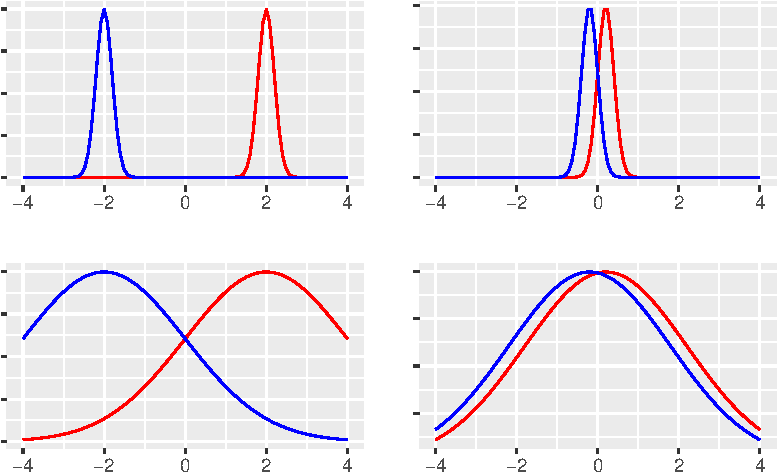
\includegraphics[keepaspectratio]{chapter08_files/figure-pdf/unnamed-chunk-4-1.pdf}}

左列は平均差が大きいデータ,右列は小さいデータである。
上段は分散が小さいデータ,下段は大きいデータである。
この4つそれぞれのシーンにおいて,「差がある」と判断しやすいのはどれかを考えてみるとよい。当然,左上のシーンが最も明確に差があると言えるであろう。なぜなら,両群が明確に分かれており,群間の重複がないからである。左下は同じ平均値差であっても,群内の広がりが大きいから群間の重複がみられるため,「差がある」という判断を受けても各群の中には該当しないケースがちらほらみられることだろう。右上パネルのようなケースでは,重複は少ないが差が小さいため,「差がある」と判断できるかどうかが微妙である。右下に至っては,差も小さく分布の重複も大きいから,「差がある」と判断しても該当しないケースが多くなる。たとえば「男性は女性よりも力が強い(体力・筋力に差がある)」というデータがあったとしても,「女性より非力な男性」もかなり多く存在するだろう。そういう反例が多くみられるような場合,統計的に差があるという結果が示されたとしても,受け入れられないのではないだろうか。

ここから明らかなように,差の判断には平均値差だけでなく分散も関わってくる。そこで平均値差を標準偏差で割った,\textbf{標準化された差}が重要になってくるのであり,これが\textbf{効果量}と呼ばれるものである\footnote{統計的な有意差よりも効果量,効果量よりも実質的な差のほうが意味のある差であることを忘れてはならない。詳しくは
  \textcite{Toyoda2009} を参照。}。

今回2群の差のデータを作る時に,\(\sigma d\)
としたが,平均値差の効果量esは, \[ es = \frac{\mu_1 - \mu_2}{\sigma} \]

で表現されるから,\(d\)が効果量を表していたのである。もちろん我々は母平均,母SDなどを知り得ないのでこれもデータから推定する他ない。幸いRには\texttt{effsize}パッケージなど,効果量を算出するものが用意されている。

\begin{Shaded}
\begin{Highlighting}[]
\NormalTok{pacman}\SpecialCharTok{::}\FunctionTok{p\_load}\NormalTok{(effsize)}
\FunctionTok{cohen.d}\NormalTok{(value }\SpecialCharTok{\textasciitilde{}}\NormalTok{ group, }\AttributeTok{data =}\NormalTok{ dataSet)}
\end{Highlighting}
\end{Shaded}

\begin{verbatim}

Cohen's d

d estimate: -0.2232655 (small)
95 percent confidence interval:
    lower     upper 
-1.165749  0.719218 
\end{verbatim}

\begin{Shaded}
\begin{Highlighting}[]
\FunctionTok{cohen.d}\NormalTok{(value }\SpecialCharTok{\textasciitilde{}}\NormalTok{ group, }\AttributeTok{data =}\NormalTok{ dataSet, }\AttributeTok{hedges.correction =} \ConstantTok{TRUE}\NormalTok{)}
\end{Highlighting}
\end{Shaded}

\begin{verbatim}

Hedges's g

g estimate: -0.2138318 (small)
95 percent confidence interval:
     lower      upper 
-1.1162608  0.6885973 
\end{verbatim}

平均値差の検定の後は,ここに示したCohenのdやHedgesのgといった効果量を添えて報告することが一般的である。

\section{対応のある二標本検定}\label{ux5bfeux5fdcux306eux3042ux308bux4e8cux6a19ux672cux691cux5b9a}

実験群と統制群のように異なる2群ではなく,プレポスト実験のように対応がある2群の場合は,t検定の定式化が異なる。対応がないt検定の場合は,群平均の差\(\mu_1 - \mu_2\)の分布を考えたが,対応がある場合は個々の測定の差,つまり\(X_{i1} - X_{i2} = D_i\)を考える。この一つの標本統計量を検定するのだから,一標本検定の一種であるとも言える。またこのDの分布の標準誤差は,標本標準誤差\(U_D\)を使った\(U_D/\sqrt{n}\)を使って推定する\footnote{対応があるケースを考えているので,当然\(n\)は前後の群で同数である。}。検定統計量\(T\)は,次式で算出される。

\[ T = \frac{\bar{D}}{U_D/\sqrt{n}} = \frac{\sum D_i/n}{\sqrt{\frac{\frac{1}{n-1}\sum(D_i-\bar{D})^2}{n}}}\]

検定にあたっては,\texttt{t.test}関数の引数\texttt{paired}を\texttt{TRUE}にするだけで良い。

\subsection{仮想データの組成}\label{ux4eeeux60f3ux30c7ux30fcux30bfux306eux7d44ux6210}

仮想データを作って演習してみよう。データの組成については,2種類のアプローチで説明が可能である。ひとつは次のシミュレーションで表されるような形である。

\begin{Shaded}
\begin{Highlighting}[]
\NormalTok{n }\OtherTok{\textless{}{-}} \DecValTok{10}
\NormalTok{mu1 }\OtherTok{\textless{}{-}} \DecValTok{4}
\NormalTok{sigma }\OtherTok{\textless{}{-}} \DecValTok{1}
\NormalTok{d }\OtherTok{\textless{}{-}} \DecValTok{1}
\NormalTok{X1 }\OtherTok{\textless{}{-}} \FunctionTok{rnorm}\NormalTok{(n, mu1, sigma)}
\NormalTok{X2 }\OtherTok{\textless{}{-}}\NormalTok{ X1 }\SpecialCharTok{+}\NormalTok{ sigma }\SpecialCharTok{*}\NormalTok{ d }\SpecialCharTok{+} \FunctionTok{rnorm}\NormalTok{(n, }\DecValTok{0}\NormalTok{, sigma)}
\FunctionTok{t.test}\NormalTok{(X1, X2, }\AttributeTok{paired =} \ConstantTok{TRUE}\NormalTok{)}
\end{Highlighting}
\end{Shaded}

\begin{verbatim}

    Paired t-test

data:  X1 and X2
t = -1.8036, df = 9, p-value = 0.1048
alternative hypothesis: true mean difference is not equal to 0
95 percent confidence interval:
 -1.4339112  0.1617193
sample estimates:
mean difference 
     -0.6360959 
\end{verbatim}

すなわち,第一の群が\(\mu_1\)を平均にばらついた実現値として得られ,第二の群はその実現値に一定の効果\(\sigma *d\)が加わり,その測定にさらに誤差がつく形である。この方法は具体的なデータ生成プロセスをそのまま模したような形でデータを作っているが,測定誤差を二重に計上している点が気になるかもしれない。

もう一つの考え方は,プレポスト型のデータに限らず,何らかの形で「対応がある」ことも表現できるものである。対応があるということは,2つのデータがそれぞれ独立した一変数正規分布から得られているのではなく,二変数正規分布から得られると考えるのである。二変数正規分布は,それぞれの変数は正規分布しているが,両者の間に相関があると考えるものである。変数が一つだけの正規分布は
\[X \sim N(\mu,\sigma)\]
で表現されているのに対し,複数の変数を同時に生成する多変数(多次元)正規分布Multivariate
Normal Distributionは,以下のように表現される。
\[ \mathbf{X} \sim MVN(\mathbf{\mu},\mathbf{\Sigma})\]

ここで\(\mathbf{X}\)や\(\mathbf{\mu}\)は\(n\)次元ベクトルであり,\(\mathbf{\Sigma}\)は分散共分散行列を表している。二変数の場合は以下のように書くことができる。

\[\mathbf{\Sigma} = \begin{pmatrix} \sigma_1^2 & \sigma_{12}\\ \sigma_{21} & \sigma_2^2 \end{pmatrix} = \begin{pmatrix} \sigma_1^2 & \rho_{12}\sigma_1\sigma_2 \\ \rho_{21}\sigma_2\sigma_1 & \sigma_2^2 \end{pmatrix}\]

共分散\(\sigma_{ij}\)は相関係数\(\rho_{ij}\)を用いて書けることからわかるように,変数間に相関があることを想定してデータを生成するのである。この組成に従った仮想データの作成は以下のとおりである。

\begin{Shaded}
\begin{Highlighting}[]
\NormalTok{pacman}\SpecialCharTok{::}\FunctionTok{p\_load}\NormalTok{(MASS) }\CommentTok{\# 多次正規乱数を生成するのに必要}
\NormalTok{n }\OtherTok{\textless{}{-}} \DecValTok{10}
\NormalTok{mu1 }\OtherTok{\textless{}{-}} \DecValTok{4}
\NormalTok{sigma }\OtherTok{\textless{}{-}} \DecValTok{1}
\NormalTok{d }\OtherTok{\textless{}{-}} \DecValTok{1}
\NormalTok{mu }\OtherTok{\textless{}{-}} \FunctionTok{c}\NormalTok{(mu1, mu1 }\SpecialCharTok{+}\NormalTok{ sigma }\SpecialCharTok{*}\NormalTok{ d)}
\NormalTok{rho }\OtherTok{\textless{}{-}} \FloatTok{0.4}
\NormalTok{SIG }\OtherTok{\textless{}{-}} \FunctionTok{matrix}\NormalTok{(}\FunctionTok{c}\NormalTok{(sigma}\SpecialCharTok{\^{}}\DecValTok{2}\NormalTok{, rho }\SpecialCharTok{*}\NormalTok{ sigma }\SpecialCharTok{*}\NormalTok{ sigma, rho }\SpecialCharTok{*}\NormalTok{ sigma }\SpecialCharTok{*}\NormalTok{ sigma, sigma}\SpecialCharTok{\^{}}\DecValTok{2}\NormalTok{), }\AttributeTok{ncol =} \DecValTok{2}\NormalTok{, }\AttributeTok{nrow =} \DecValTok{2}\NormalTok{)}
\NormalTok{X }\OtherTok{\textless{}{-}} \FunctionTok{mvrnorm}\NormalTok{(n, mu, SIG)}
\FunctionTok{t.test}\NormalTok{(X[, }\DecValTok{1}\NormalTok{], X[, }\DecValTok{2}\NormalTok{], }\AttributeTok{paired =} \ConstantTok{TRUE}\NormalTok{)}
\end{Highlighting}
\end{Shaded}

\begin{verbatim}

    Paired t-test

data:  X[, 1] and X[, 2]
t = -2.4313, df = 9, p-value = 0.0379
alternative hypothesis: true mean difference is not equal to 0
95 percent confidence interval:
 -1.96934592 -0.07095313
sample estimates:
mean difference 
       -1.02015 
\end{verbatim}

効果量については,対応のないt検定の場合と同じで良い。

\begin{Shaded}
\begin{Highlighting}[]
\FunctionTok{cohen.d}\NormalTok{(X[, }\DecValTok{1}\NormalTok{], X[, }\DecValTok{2}\NormalTok{])}
\end{Highlighting}
\end{Shaded}

\begin{verbatim}

Cohen's d

d estimate: -1.04088 (large)
95 percent confidence interval:
      lower       upper 
-2.04204357 -0.03971697 
\end{verbatim}

\begin{Shaded}
\begin{Highlighting}[]
\FunctionTok{cohen.d}\NormalTok{(X[, }\DecValTok{1}\NormalTok{], X[, }\DecValTok{2}\NormalTok{], }\AttributeTok{hedges.correction =} \ConstantTok{TRUE}\NormalTok{)}
\end{Highlighting}
\end{Shaded}

\begin{verbatim}

Hedges's g

g estimate: -0.9968994 (large)
95 percent confidence interval:
     lower      upper 
-1.9510179 -0.0427809 
\end{verbatim}

\subsection{検定の方向性}\label{ux691cux5b9aux306eux65b9ux5411ux6027}

ここまでの検定では,主に「差があるかどうか」といった仮説に対応するものを扱ってきた。差があるかどうか,というのはその差がプラスの方向にでているのか,マイナスの方向に出ているのかといったことを問題にしていない。そこで検定統計量の分布についても,分布の両裾を考えて有意水準を設定していた。

しかしプレポスト実験などでは,効果が「上がった」のか「下がった」のか,ということが大きな関心時でもあることが多いだろう。効果がある,ただし逆効果である,というのでは意味がないからである。このように方向性をもった仮説を検証する場合は,検定統計量の分布も一方向だけ考えればよく,\texttt{t.test}関数には\texttt{alternative}オプションをつかって表現する。

\texttt{t.test(x,y,alternatives\ =\ "less")}
とすると\(x < y\)の帰無仮説を検証することになるし,\texttt{alternatives\ =\ "greater"}とすると\(x > y\)の帰無仮説を検証することになる。デフォルトでは\texttt{alternatives\ =\ "two.sided"}であり,両側検定が選ばれている。

ただし,両裾から片裾にかわるということは,検定統計量が超えるかどうかの判断をする\textbf{臨界値}が小さくなることでもある。必然的に,片裾(片側検定)のほうが緩やかな基準で検定をしていることにもなる。デフォルトで普段から厳しく検定しているから大丈夫だろう,というのも一つの考え方だが,やはり本来の研究仮説に適した帰無仮説の設定をするべきだろう。

\section{課題}\label{ux8ab2ux984c-6}

\begin{enumerate}
\def\labelenumi{\arabic{enumi}.}
\item
  平均が50、標準偏差が10の正規分布からランダムに選んだ30個のサンプルを用意し,このサンプルの平均が母集団の平均と異なるかどうかを検定してください。検定結果を,心理学のフォーマット(心理学会編「論文執筆投稿の手引き」)に準拠した書き方で,結果を記述してください。
\item
  以下のデータセットを使用して,2つの独立した群の平均に差があるかどうかをt検定してください。検定結果を,心理学のフォーマット(心理学会編「論文執筆投稿の手引き」)に準拠した書き方で,結果を記述してください。
  \[ group1 =\{45, 50, 55, 60, 65 \} \]
  \[ group2 = \{57, 60, 62, 77, 75 \} \]
\item
  多次元正規分布を用いた仮想データ生成方で,対応のあるt検定の練習をしましょう。サンプルサイズを\(n=20\)とし,
  平均ベクトル\(\mu = (12, 15)\),
  分散共分散行列\(\Sigma = \begin{pmatrix} 4 & 2.8 \\ 2.8 & 4\end{pmatrix}\)の多次元正規分布から作られた乱数を使って,対応のあるt検定をしてください。検定結果を,心理学のフォーマット(心理学会編「論文執筆投稿の手引き」)に準拠した書き方で,結果を記述してください。
\item
  自由度が10, 20,
  30のt分布のグラフを,標準正規分布のグラフとともに描画してください。自由度が増えるとt分布がどのように変化するでしょうか。
\item
  自由度が15のt分布において、有意水準5\%の片側検定と両側検定の臨界値(検定の判断基準となる理論値)を求めてください。
\end{enumerate}

\bookmarksetup{startatroot}

\chapter{多群の平均値差の検定}\label{ux591aux7fa4ux306eux5e73ux5747ux5024ux5deeux306eux691cux5b9a}

心理学実験においては,古典的に分散分析モデルが多用されてきた。平均値差を見ることで実験の効果,因果関係を明らかにできるように,巧妙に実験デザインが組み立てられる。その精緻さは理論的一貫性という意味である種の美しさを持ち,多くの研究者が魅了されてきた。

分散分析にのせることを目的にした実験計画であり,実験デザインの不自由さ(とにかく分散分析をしなければならない!)が批判的に論じられることもあるが,心理学が測定している対象が平均値差以上の精度で議論できる性質でないという反論もあるだろう。

今や分散分析を超えたより高度な統計モデルがあり,現在の研究においては分散分析はもはや過去のものにすぎないかもしれないが,以後のモデルも分散分析を基本としたその発展系であるので,改めて基本を押さえておくことも重要である。

\section{分散分析の基礎}\label{ux5206ux6563ux5206ux6790ux306eux57faux790e}

分散分析は「分散」の分析であるかのような名称であるが,平均値差を検定するためのものである。なぜ「分散」を冠するかといえば,効果量のところで見たように,平均値差の判断には群内分散の情報が必要だからである。

多群の平均値の差,その散らばりを群間分散といい,群に含まれるデータの散らばりを群内分散とよぶ。分散分析は群内分散に対する群間分散の比が十分に大きいと考えられる場合,群間に統計的な有意差があると判断する。分散の比を表す確率分布はF分布と呼ばれる。F分布は群間・群内それぞれの自由度を母数にもつ。

また,実験計画はBetweenデザインとWithinデザインに区分される。t検定でみたような,対応のない独立した群を対象にしたデザインがBetween,群間に相関が想定される対応のある群を対象にしたデザインがWithinである。Withinデザインは同じ個体から複数回の反応を得る(ex.
period 1-2-3\ldots)ため,反復測定デザインRepeated measured
designともよばれることがある。この場合,群内分散から個人内の分散すなわち個人差を取り出すことができるため,これが分離できないBetweenデザインよりも基本的にWithinデザインのほうが目的となる変動を捉えやすい。ただし,反復測定による個体への負担を考えると,毎回Withinデザインでいいというわけにもいかないところが難点である。

\[Between Design: \text{全変動} = \text{群間変動}+ \text{群内変動(誤差)}\]
\[Within Design:  \text{全変動} = \text{群間変動}+ \text{個人差変動} + \text{誤差}\]

分散分析は要因が複数ある場合も考えられるから,要因AがBetween,要因BがWithinといった場合は混合計画と呼ばれることがある。慣例的に,要因Factorとその要因に含まれる水準Levelを同時に表現し,\(\text{間}2 \times \text{間}3\)の分散分析(二要因の分散分析で,いずれもBetweenデザインであり,水準数がそれぞれ2と3),といった言い方をすることがある。

\section{分散分析のステップ}\label{ux5206ux6563ux5206ux6790ux306eux30b9ux30c6ux30c3ux30d7}

t検定において等分散性の仮定が成立するかどうかが事前に問題になったように,Betweenデザインにおいても分散の等質性は仮定されており,Leveneの検定などで事前に検証しておくべきである。またWithinデザインにおいては,データの組成に関わる分散共分散行列の非対角要素が全て等しいことが望ましいが,実践的にはそこまでの仮定が成立しているとは考えにくい。ただし分散分析としては,等分散性の仮定よりも,より緩やかな球面性の仮定が成立していればよいとされており,これを事前に検定することが一般的である。Welchの補正のように,球面性の仮定が成立していない場合は,自由度を補正することで検定の精度が維持される。

分散分析は多要因・多水準の平均値差の検定である。各水準ごとにt検定を繰り返せば良いのではないか,というアイデアは誰しも思いつくことであろうが,この方法は検定の目的である\(\alpha\)水準の制御ができなくなるという問題を含む。そこで多水準の場合は分散分析を行うことで,すべての要因・水準の母平均が同じであるという帰無仮説を検定し,効果の有無をまず明確にする。この帰無仮説が棄却されたらどこかに差があるわけだから,以後は慎重に\(\alpha\)水準を制御しつつ事後的な検定にすすむ。

水準間の差をみるための事後的な検定は,下位検定とも呼ばれる。その方法は多岐に渡り,ゴールドスタンダードは存在せず,往々にして分析者が利用しているソフトウェアが対応する手法が選択される。要因・水準が多くなると検証すべき組み合わせも多くなり,下位検定の手続きも非常に煩雑になる。統計ソフトウェアはそれこそ機械的に,幾重にも細かく分散分析表を分解して下位検定をつづけていってくれるが,いくら制御されているとはいえ検定を繰り返していることに変わりはないし,各下位検定の結果を一貫した総合的解釈をするのは困難である。実験計画はシンプルであるほうが望ましいし,複雑なモデルになるようであれば分散分析を超えた,階層線形モデルやベイジアンアプローチなどを取る方が良いだろう。

\section{ANOVA君を使う}\label{anovaux541bux3092ux4f7fux3046}

分散分析をRで実行するには,基本関数である\texttt{aov}やcarパッケージなどを用いることができる。
もっとも,その出力は必ずしも親切ではないし,下位検定や効果量の算出などは別のパッケージ,別の関数を用いる必要がある。

筆者がお勧めするのは,大正大学の井関龍太が開発した\href{https://riseki.cloudfree.jp/?ANOVA君}{anovakun}である。パッケージ化されていないので,リンク先からソースコードを読み込んでanovakun関数を実行する必要があるが,さまざまな実験デザインに対応し,また下位検定や効果量,球面性の補正などおよそ分散分析で必要な手法は網羅されている。以下ではこれを用いた実践を行う。

anovakunの読み込みは,ソースコードをプロジェクトフォルダにダウンロードして\texttt{source}関数で読み込むか,インターネットに繋がっている状態でリンク先から直接ソースファイル(anovakun\_489.txt)\footnote{2024.03.17時点での最新バージョンが4.8.9である。リンク先URLは,公式サイトからソースファイルのリンクをコピーして貼り付けると良い。}を\texttt{source}関数で読み込むといいだろう。

\begin{Shaded}
\begin{Highlighting}[]
\FunctionTok{source}\NormalTok{(}\StringTok{"https://riseki.cloudfree.jp/?plugin=attach\&refer=ANOVA\%E5\%90\%9B\&openfile=anovakun\_489.txt"}\NormalTok{)}
\end{Highlighting}
\end{Shaded}

読み込みが終わるとEnvironタブにanovakun関数が含まれていることを確認しよう。

\subsection{ANOVA君の入力とデータ}\label{anovaux541bux306eux5165ux529bux3068ux30c7ux30fcux30bf}

ANOVA君は伝統的にワイド型データから読み込むようになっている。すなわち,一行に1オブザベーション入っている形式である。Between計画の場合は,データの前に水準数を表すインデックスと最終的な従属変数の形に整形したデータが必要である。Within計画の場合は1行に1Obs.なのだから,反復した水準の数だけ右にデータを入れていく形に整形する。

しかしChapter~\ref{sec-Long_and_Wide}
で述べたように,昨今は計算機にとって優しい型,ロング型での入力もおおく,ANOVA君もversion
4.4.0からロング型での入力も許すようになった。その場合はオプション\texttt{long=TRUE}
とロング型であることを明記する必要がある。

ANOVA君を使う時は,関数\texttt{anovakun}に,データ,要因計画の型,各要因の水準の順で入力する。ここで要因計画の型とは,文字列でBetween/Withinの違いを明示することになる。被験者のラベルを表す小文字の\texttt{s}を挟んで,左側に間(Between)要因,右側に内(Within)要因を入れる。例えば一要因Between計画の場合は\texttt{"As"},二要因Within計画の場合は\texttt{"sAB"},間1内2の混合計画であれば\texttt{"AsBC"}のようにする。

続いて入力する水準数は,要因の数だけ必要である。ただし,ロング型で入力した場合は自動的に水準数が計算されるので入力の必要がない。

このテキストでは,データの持ち替えについてすでに触れているので,色々扱いやすいロング型に整形して利用していくものとする。

\section{Betweenデザイン}\label{betweenux30c7ux30b6ux30a4ux30f3}

\subsection{1way-ANOVA}\label{way-anova}

もっとも単純な一要因3水準,Between計画の例から始めよう。仮想データの生成を行うことで,分散分析のメカニズムと共に見ていくことにする。

\begin{Shaded}
\begin{Highlighting}[]
\FunctionTok{set.seed}\NormalTok{(}\DecValTok{123}\NormalTok{)}
\CommentTok{\# 各群のサンプルサイズ}
\NormalTok{n1 }\OtherTok{\textless{}{-}} \DecValTok{5}
\NormalTok{n2 }\OtherTok{\textless{}{-}} \DecValTok{4}
\NormalTok{n3 }\OtherTok{\textless{}{-}} \DecValTok{6}
\CommentTok{\# 母平均,効果量,母SD}
\NormalTok{mu }\OtherTok{\textless{}{-}} \DecValTok{10}
\NormalTok{delta }\OtherTok{\textless{}{-}} \DecValTok{1}
\NormalTok{sigma }\OtherTok{\textless{}{-}} \DecValTok{3}
\CommentTok{\# 群平均}
\NormalTok{mu1 }\OtherTok{\textless{}{-}}\NormalTok{ mu }\SpecialCharTok{{-}}\NormalTok{ (delta }\SpecialCharTok{*}\NormalTok{ sigma)}
\NormalTok{mu2 }\OtherTok{\textless{}{-}}\NormalTok{ mu}
\NormalTok{mu3 }\OtherTok{\textless{}{-}}\NormalTok{ mu }\SpecialCharTok{+}\NormalTok{ (delta }\SpecialCharTok{*}\NormalTok{ sigma)}
\CommentTok{\# データセット}
\NormalTok{X1 }\OtherTok{\textless{}{-}} \FunctionTok{rnorm}\NormalTok{(n1, mu1, sigma)}
\NormalTok{X2 }\OtherTok{\textless{}{-}} \FunctionTok{rnorm}\NormalTok{(n2, mu2, sigma)}
\NormalTok{X3 }\OtherTok{\textless{}{-}} \FunctionTok{rnorm}\NormalTok{(n3, mu3, sigma)}
\DocumentationTok{\#\# 組み上げる}
\NormalTok{dat }\OtherTok{\textless{}{-}} \FunctionTok{data.frame}\NormalTok{(}
  \AttributeTok{ID =} \DecValTok{1}\SpecialCharTok{:}\NormalTok{(n1 }\SpecialCharTok{+}\NormalTok{ n2 }\SpecialCharTok{+}\NormalTok{ n3),}
  \AttributeTok{group =} \FunctionTok{as.factor}\NormalTok{(}\FunctionTok{rep}\NormalTok{(LETTERS[}\DecValTok{1}\SpecialCharTok{:}\DecValTok{3}\NormalTok{], }\FunctionTok{c}\NormalTok{(n1, n2, n3))),}
  \AttributeTok{value =} \FunctionTok{c}\NormalTok{(X1, X2, X3)}
\NormalTok{)}
\DocumentationTok{\#\# データの確認}
\NormalTok{dat}
\end{Highlighting}
\end{Shaded}

\begin{verbatim}
   ID group     value
1   1     A  5.318573
2   2     A  6.309468
3   3     A 11.676125
4   4     A  7.211525
5   5     A  7.387863
6   6     B 15.145195
7   7     B 11.382749
8   8     B  6.204816
9   9     B  7.939441
10 10     C 11.663014
11 11     C 16.672245
12 12     C 14.079441
13 13     C 14.202314
14 14     C 13.332048
15 15     C 11.332477
\end{verbatim}

\begin{Shaded}
\begin{Highlighting}[]
\DocumentationTok{\#\#\# 実行}
\FunctionTok{anovakun}\NormalTok{(dat, }\StringTok{"As"}\NormalTok{, }\AttributeTok{long =} \ConstantTok{TRUE}\NormalTok{, }\AttributeTok{peta =} \ConstantTok{TRUE}\NormalTok{)}
\end{Highlighting}
\end{Shaded}

\begin{verbatim}

[ As-Type Design ]

This output was generated by anovakun 4.8.9 under R version 4.5.0.
It was executed on Fri Jun 13 15:02:04 2025.

 
<< DESCRIPTIVE STATISTICS >>

------------------------------
 group   n     Mean    S.D. 
------------------------------
     A   5   7.5807  2.4331 
     B   4  10.1681  3.9548 
     C   6  13.5469  1.9483 
------------------------------


<< ANOVA TABLE >>

== This data is UNBALANCED!! ==
== Type III SS is applied. ==

--------------------------------------------------------------
 Source       SS  df      MS  F-ratio  p-value      p.eta^2 
--------------------------------------------------------------
  group  98.3840   2 49.1920   6.5897   0.0117 *     0.5234 
  Error  89.5804  12  7.4650                                
--------------------------------------------------------------
  Total 187.9644  14 13.4260                                
                  +p < .10, *p < .05, **p < .01, ***p < .001


<< POST ANALYSES >>

< MULTIPLE COMPARISON for "group" >

== Shaffer's Modified Sequentially Rejective Bonferroni Procedure ==
== The factor < group > is analysed as independent means. == 
== Alpha level is 0.05. == 
 
------------------------------
 group   n     Mean    S.D. 
------------------------------
     A   5   7.5807  2.4331 
     B   4  10.1681  3.9548 
     C   6  13.5469  1.9483 
------------------------------

-------------------------------------------------------
 Pair     Diff  t-value  df       p   adj.p          
-------------------------------------------------------
  A-C  -5.9662   3.6062  12  0.0036  0.0108  A < C * 
  B-C  -3.3789   1.9159  12  0.0795  0.0795  B = C   
  A-B  -2.5873   1.4117  12  0.1834  0.1834  A = B   
-------------------------------------------------------


output is over --------------------///
\end{verbatim}

出力結果は大きく分けて記述統計\texttt{\textless{}\textless{}\ DESCRIPTIVE\ STATISTICS\ \textgreater{}\textgreater{}}と,分散分析表\texttt{\textless{}\textless{}\ ANOVA\ TABLE\ \textgreater{}\textgreater{}},下位検定\texttt{\textless{}\textless{}\ POST\ ANALYSES\ \textgreater{}\textgreater{}}に分けられる。記述統計はデータが正しく読み込めているかどうかのチェックに使おう。

一番のメインは分散分析表であり,平方和sum of
squaresを自由度dfで割った,1自由度あたりのデータの散らばりを,群間と群内(誤差)との比で検証しているのが見て取れる。群間平方和が\(98.38\),群内平方和が\(89.58\)であり,それぞれ自由度\(2\)(\(3\)水準\(-1\))と\(12\)(\(\sum_{j=1}^3 n_j-1\))から生じているので,平均平方Mean
Squaresがそれぞれ\(49.19\)と\(7.47\)である。この比が\(6.5897\)で,自由度\(F(2,12)\)のF分布においてこの値以上の極端な数字が出る確率が5\%を下回っている(実に\(p=0.0117\)である)ため,統計的に有意であると判断できる。
分散分析表のTotalのところで,全体のSSが群間SS+群内SSに一致していること,自由度も全体df=群間df+群内dfになっていることを確認しておこう。

また,\texttt{anovakun}関数の引数として\texttt{peta\ =\ TRUE}を指定したが,これは偏\(\eta^2\)(partial
eta)と呼ばれる効果量を出力するためのオプションである。

今回は分散分析の時点で統計的な有意差が認められたため(\(F(2,12)=6.59, p < 0.05, \eta^2=0.52\)),続いて下位検定が表示されている。ANOVA君は下位検定についても複数のオプションを持っているが,デフォルトではShafferの修正Bonferroni検定が行われる。詳しくは専門書\autocite{Nagata.kentei}を参照してほしいが,概略を説明すると,検証すべき仮説の数で有意水準を分割するというBonferroniの方法を,競合する仮説の数も考慮して分母を調整するというものである。

この計算の結果,A群とC群の間にのみ統計的な有意差が確認された(\(t(12)=3.61,p<0.05\))と言える。

\subsection{2way-ANOVA}\label{way-anova-1}

二要因の場合も見ておこう。ANOVA君の表記方法は要因計画の型が変わるだけで大きな変更はないが,交互作用interactionを考える必要があるところがポイントである。これも仮想データの組成を見ることでその意義がわかりやすくなるだろう。間2\(\times\)間2の実験デザインを例に,まずは各水準の理論的平均値がどのようにつくられるかをみておこう。

\begin{Shaded}
\begin{Highlighting}[]
\FunctionTok{set.seed}\NormalTok{(}\DecValTok{123}\NormalTok{)}
\CommentTok{\# 各群のサンプルサイズ}
\NormalTok{n }\OtherTok{\textless{}{-}} \DecValTok{10}
\CommentTok{\# 全体平均,効果量,母SD}
\NormalTok{mu }\OtherTok{\textless{}{-}} \DecValTok{10}
\NormalTok{delta1 }\OtherTok{\textless{}{-}} \DecValTok{1}
\NormalTok{delta2 }\OtherTok{\textless{}{-}} \DecValTok{0} \CommentTok{\# ここではあえて要因Bの効果を0にしている}
\NormalTok{delta3 }\OtherTok{\textless{}{-}} \DecValTok{2}
\NormalTok{sigma }\OtherTok{\textless{}{-}} \DecValTok{3}
\CommentTok{\# 効果の計算}
\NormalTok{effectA }\OtherTok{\textless{}{-}}\NormalTok{ delta1 }\SpecialCharTok{*}\NormalTok{ sigma }\CommentTok{\# Factor A}
\NormalTok{effectB }\OtherTok{\textless{}{-}}\NormalTok{ delta2 }\SpecialCharTok{*}\NormalTok{ sigma }\CommentTok{\# Factor B}
\NormalTok{effectAB }\OtherTok{\textless{}{-}}\NormalTok{ delta3 }\SpecialCharTok{*}\NormalTok{ sigma }\CommentTok{\# interaction}
\CommentTok{\# 各群の平均}
\NormalTok{mu11 }\OtherTok{\textless{}{-}}\NormalTok{ mu }\SpecialCharTok{+}\NormalTok{ effectA }\SpecialCharTok{+}\NormalTok{ effectB }\SpecialCharTok{+}\NormalTok{ effectAB}
\NormalTok{mu12 }\OtherTok{\textless{}{-}}\NormalTok{ mu }\SpecialCharTok{+}\NormalTok{ effectA }\SpecialCharTok{{-}}\NormalTok{ effectB }\SpecialCharTok{{-}}\NormalTok{ effectAB}
\NormalTok{mu21 }\OtherTok{\textless{}{-}}\NormalTok{ mu }\SpecialCharTok{{-}}\NormalTok{ effectA }\SpecialCharTok{+}\NormalTok{ effectB }\SpecialCharTok{{-}}\NormalTok{ effectAB}
\NormalTok{mu22 }\OtherTok{\textless{}{-}}\NormalTok{ mu }\SpecialCharTok{{-}}\NormalTok{ effectA }\SpecialCharTok{{-}}\NormalTok{ effectB }\SpecialCharTok{+}\NormalTok{ effectAB}
\end{Highlighting}
\end{Shaded}

効果の現れ方は相対的だから,要因Aが第一水準に\texttt{+effectA}の形で現れたら,第二水準には\texttt{-effectA}
の形で現れる。要因Bについても同様である。交互作用については組み合わせにおいて生じるから,要因Aの第一水準と要因Bの第一水準の組み合わせのところに\texttt{+effectAB}を充てる。ここでも効果は相対的に現れるという条件を守るために,要因Aの第一水準の中で\texttt{+effectAB}の効果を相殺するために,要因Aの第一水準と要因Bの第二水準の組み合わせの符号が反転する。同様に,要因Bの第一水準の中で相殺するために要因Aの第二水準と要因Bの第一水準には\texttt{-effectAB}が加わる。

このようにして考えられる理論的平均値に対して,外乱要因である誤差が生じて実現値が得られる。
組み上げて得られたデータを確認しておこう。

\begin{Shaded}
\begin{Highlighting}[]
\NormalTok{X11 }\OtherTok{\textless{}{-}} \FunctionTok{rnorm}\NormalTok{(n, }\AttributeTok{mean =}\NormalTok{ mu11, }\AttributeTok{sd =}\NormalTok{ sigma)}
\NormalTok{X12 }\OtherTok{\textless{}{-}} \FunctionTok{rnorm}\NormalTok{(n, }\AttributeTok{mean =}\NormalTok{ mu12, }\AttributeTok{sd =}\NormalTok{ sigma)}
\NormalTok{X21 }\OtherTok{\textless{}{-}} \FunctionTok{rnorm}\NormalTok{(n, }\AttributeTok{mean =}\NormalTok{ mu21, }\AttributeTok{sd =}\NormalTok{ sigma)}
\NormalTok{X22 }\OtherTok{\textless{}{-}} \FunctionTok{rnorm}\NormalTok{(n, }\AttributeTok{mean =}\NormalTok{ mu22, }\AttributeTok{sd =}\NormalTok{ sigma)}
\NormalTok{dat }\OtherTok{\textless{}{-}} \FunctionTok{data.frame}\NormalTok{(}
  \AttributeTok{ID =} \DecValTok{1}\SpecialCharTok{:}\NormalTok{(n }\SpecialCharTok{*} \DecValTok{4}\NormalTok{),}
  \AttributeTok{FactorA =} \FunctionTok{rep}\NormalTok{(}\DecValTok{1}\SpecialCharTok{:}\DecValTok{2}\NormalTok{, }\AttributeTok{each =}\NormalTok{ n }\SpecialCharTok{*} \DecValTok{2}\NormalTok{),}
  \AttributeTok{FactorB =} \FunctionTok{rep}\NormalTok{(}\FunctionTok{rep}\NormalTok{(}\DecValTok{1}\SpecialCharTok{:}\DecValTok{2}\NormalTok{, }\AttributeTok{each =}\NormalTok{ n), }\DecValTok{2}\NormalTok{),}
  \AttributeTok{value =} \FunctionTok{c}\NormalTok{(X11, X12, X21, X22)}
\NormalTok{)}
\NormalTok{dat}
\end{Highlighting}
\end{Shaded}

\begin{verbatim}
   ID FactorA FactorB      value
1   1       1       1 17.3185731
2   2       1       1 18.3094675
3   3       1       1 23.6761249
4   4       1       1 19.2115252
5   5       1       1 19.3878632
6   6       1       1 24.1451950
7   7       1       1 20.3827486
8   8       1       1 15.2048163
9   9       1       1 16.9394414
10 10       1       1 17.6630141
11 11       1       2 10.6722454
12 12       1       2  8.0794415
13 13       1       2  8.2023144
14 14       1       2  7.3320481
15 15       1       2  5.3324766
16 16       1       2 12.3607394
17 17       1       2  8.4935514
18 18       1       2  1.1001485
19 19       1       2  9.1040677
20 20       1       2  5.5816258
21 21       2       1 -2.2034711
22 22       2       1  0.3460753
23 23       2       1 -2.0780133
24 24       2       1 -1.1866737
25 25       2       1 -0.8751178
26 26       2       1 -4.0600799
27 27       2       1  3.5133611
28 28       2       1  1.4601194
29 29       2       1 -2.4144108
30 30       2       1  4.7614448
31 31       2       2 14.2793927
32 32       2       2 12.1147856
33 33       2       2 15.6853770
34 34       2       2 15.6344005
35 35       2       2 15.4647432
36 36       2       2 15.0659208
37 37       2       2 14.6617530
38 38       2       2 12.8142649
39 39       2       2 12.0821120
40 40       2       2 11.8585870
\end{verbatim}

もちろん実際には,計画に応じたデータセットが得られているはずであり,各群のサンプルサイズが異なるなどの事情もあるだろう。しかしこうして,理論的にデータの組成を見ておくことで,サンプルサイズを変えたり効果量を変えたりしながら,どのように結果が変わってくるかを確認しながら進めることができる\footnote{かつては分散分析は手計算でできる分析モデルであり,得られたデータを平方和に分解していくプロセスをたどりながら分散分析のメカニズムが体得されるという教育が多く見られた。ただしその方法は計算に時間がかかること,ミスが混在しやすいことに加え,手元のデータが唯一無二のものであるという印象を強くすることが懸念される。推測統計学においては,手元のデータはあくまでも実現値に過ぎないと考えるのであり,乱数を生成して幾つでも自在に作り出せる経験を得た方が教育効果として良いのではないか,と筆者は考えている。}。

それではこの仮想データを分析してみよう。

\begin{Shaded}
\begin{Highlighting}[]
\FunctionTok{anovakun}\NormalTok{(dat, }\StringTok{"ABs"}\NormalTok{, }\AttributeTok{long =} \ConstantTok{TRUE}\NormalTok{, }\AttributeTok{peta =} \ConstantTok{TRUE}\NormalTok{)}
\end{Highlighting}
\end{Shaded}

\begin{verbatim}

[ ABs-Type Design ]

This output was generated by anovakun 4.8.9 under R version 4.5.0.
It was executed on Fri Jun 13 15:02:05 2025.

 
<< DESCRIPTIVE STATISTICS >>

-----------------------------------------
 FactorA  FactorB   n     Mean    S.D. 
-----------------------------------------
       1        1  10  19.2239  2.8614 
       1        2  10   7.6259  3.1142 
       2        1  10  -0.2737  2.7924 
       2        2  10  13.9661  1.5819 
-----------------------------------------


<< ANOVA TABLE >>

---------------------------------------------------------------------------
           Source        SS  df        MS  F-ratio  p-value      p.eta^2 
---------------------------------------------------------------------------
          FactorA  432.7854   1  432.7854  61.4190   0.0000 ***   0.6305 
          FactorB   17.4478   1   17.4478   2.4761   0.1243 ns    0.0644 
FactorA x FactorB 1668.9825   1 1668.9825 236.8545   0.0000 ***   0.8681 
            Error  253.6721  36    7.0464                                
---------------------------------------------------------------------------
            Total 2372.8878  39   60.8433                                
                               +p < .10, *p < .05, **p < .01, ***p < .001


<< POST ANALYSES >>

< SIMPLE EFFECTS for "FactorA x FactorB" INTERACTION >

----------------------------------------------------------------------
      Source        SS  df        MS  F-ratio  p-value      p.eta^2 
----------------------------------------------------------------------
FactorA at 1 1900.7730   1 1900.7730 269.7492   0.0000 ***   0.8823 
FactorA at 2  200.9950   1  200.9950  28.5243   0.0000 ***   0.4421 
FactorB at 1  672.5693   1  672.5693  95.4480   0.0000 ***   0.7261 
FactorB at 2 1013.8610   1 1013.8610 143.8826   0.0000 ***   0.7999 
       Error  253.6721  36    7.0464                                
----------------------------------------------------------------------
                          +p < .10, *p < .05, **p < .01, ***p < .001

output is over --------------------///
\end{verbatim}

基本的な結果の見方については,一要因のときと同じである。今回は要因Aと交互作用の効果を作り,正しく検出されている。下位検定については,要因Aが2水準であったためこちらの主効果の検証は必要なく(記述統計を見て群平均比較をすればよい),交互作用についての単純効果の検証が行われている。

\section{Withinデザイン}\label{withinux30c7ux30b6ux30a4ux30f3}

Withinデザインは対応のあるt検定の時と同じように,多次元正規分布からの生成として考えよう。すなわち各個体から得られるデータが相関しているという仮定をおくのである。以下のサンプルコードを読んで,データ生成過程を確認しよう。なお共分散は\(\rho_{xy}=\frac{s_{xy}}{s_xs_y}\)より\(s_{xy}=\rho_{xy}s_xs_y\)として整形している。

\begin{Shaded}
\begin{Highlighting}[]
\NormalTok{pacman}\SpecialCharTok{::}\FunctionTok{p\_load}\NormalTok{(tidyverse)}
\NormalTok{pacman}\SpecialCharTok{::}\FunctionTok{p\_load}\NormalTok{(MASS)}
\FunctionTok{set.seed}\NormalTok{(}\DecValTok{42}\NormalTok{)}
\CommentTok{\# 各群のサンプルサイズ}
\NormalTok{n }\OtherTok{\textless{}{-}} \DecValTok{10}
\CommentTok{\# 全体平均,効果量,母SD}
\NormalTok{mu }\OtherTok{\textless{}{-}} \DecValTok{10}
\NormalTok{delta }\OtherTok{\textless{}{-}} \DecValTok{1}
\NormalTok{s1 }\OtherTok{\textless{}{-}}\NormalTok{ s2 }\OtherTok{\textless{}{-}}\NormalTok{ s3 }\OtherTok{\textless{}{-}} \DecValTok{1}
\NormalTok{rho12 }\OtherTok{\textless{}{-}} \FloatTok{0.1}
\NormalTok{rho13 }\OtherTok{\textless{}{-}} \FloatTok{0.3}
\NormalTok{rho23 }\OtherTok{\textless{}{-}} \FloatTok{0.8}
\NormalTok{mus }\OtherTok{\textless{}{-}} \FunctionTok{c}\NormalTok{(mu, mu }\SpecialCharTok{+}\NormalTok{ s1 }\SpecialCharTok{*}\NormalTok{ delta, mu }\SpecialCharTok{{-}}\NormalTok{ s1 }\SpecialCharTok{*}\NormalTok{ delta)}
\CommentTok{\# 共分散行列の生成}
\NormalTok{Sigma }\OtherTok{\textless{}{-}} \FunctionTok{matrix}\NormalTok{(}\ConstantTok{NA}\NormalTok{, }\AttributeTok{ncol =} \DecValTok{3}\NormalTok{, }\AttributeTok{nrow =} \DecValTok{3}\NormalTok{)}
\NormalTok{Sigma[}\DecValTok{1}\NormalTok{, }\DecValTok{1}\NormalTok{] }\OtherTok{\textless{}{-}}\NormalTok{ s1}\SpecialCharTok{\^{}}\DecValTok{2}
\NormalTok{Sigma[}\DecValTok{2}\NormalTok{, }\DecValTok{2}\NormalTok{] }\OtherTok{\textless{}{-}}\NormalTok{ s2}\SpecialCharTok{\^{}}\DecValTok{2}
\NormalTok{Sigma[}\DecValTok{3}\NormalTok{, }\DecValTok{3}\NormalTok{] }\OtherTok{\textless{}{-}}\NormalTok{ s3}\SpecialCharTok{\^{}}\DecValTok{2}
\NormalTok{Sigma[}\DecValTok{1}\NormalTok{, }\DecValTok{2}\NormalTok{] }\OtherTok{\textless{}{-}}\NormalTok{ Sigma[}\DecValTok{2}\NormalTok{, }\DecValTok{1}\NormalTok{] }\OtherTok{\textless{}{-}}\NormalTok{ rho12 }\SpecialCharTok{*}\NormalTok{ s1 }\SpecialCharTok{*}\NormalTok{ s2}
\NormalTok{Sigma[}\DecValTok{1}\NormalTok{, }\DecValTok{3}\NormalTok{] }\OtherTok{\textless{}{-}}\NormalTok{ Sigma[}\DecValTok{3}\NormalTok{, }\DecValTok{1}\NormalTok{] }\OtherTok{\textless{}{-}}\NormalTok{ rho13 }\SpecialCharTok{*}\NormalTok{ s1 }\SpecialCharTok{*}\NormalTok{ s3}
\NormalTok{Sigma[}\DecValTok{2}\NormalTok{, }\DecValTok{3}\NormalTok{] }\OtherTok{\textless{}{-}}\NormalTok{ Sigma[}\DecValTok{3}\NormalTok{, }\DecValTok{2}\NormalTok{] }\OtherTok{\textless{}{-}}\NormalTok{ rho23 }\SpecialCharTok{*}\NormalTok{ s2 }\SpecialCharTok{*}\NormalTok{ s3}
\CommentTok{\# データの生成}
\NormalTok{X }\OtherTok{\textless{}{-}} \FunctionTok{mvrnorm}\NormalTok{(n, mus, Sigma) }\SpecialCharTok{\%\textgreater{}\%} \FunctionTok{as.data.frame}\NormalTok{()}
\CommentTok{\# データの確認}
\NormalTok{X}
\end{Highlighting}
\end{Shaded}

\begin{verbatim}
          V1        V2       V3
1  10.625304  9.418518 7.493325
2  12.437964 11.249993 8.806719
3   8.604481 11.182418 8.722798
4   9.390742 10.181310 8.786312
5   9.567609 10.147592 9.194809
6  10.651739 11.005419 8.917299
7   9.125913  9.805634 7.511082
8   7.770294 12.462671 8.790231
9   6.909722  9.863405 7.429485
10 11.267590 10.798088 8.754522
\end{verbatim}

\begin{Shaded}
\begin{Highlighting}[]
\CommentTok{\# Long型に整形}
\NormalTok{X }\OtherTok{\textless{}{-}}\NormalTok{ X }\SpecialCharTok{\%\textgreater{}\%}
  \FunctionTok{rowid\_to\_column}\NormalTok{(}\StringTok{"ID"}\NormalTok{) }\SpecialCharTok{\%\textgreater{}\%}
  \FunctionTok{pivot\_longer}\NormalTok{(}\SpecialCharTok{{-}}\NormalTok{ID) }\SpecialCharTok{\%\textgreater{}\%}
  \FunctionTok{print}\NormalTok{()}
\end{Highlighting}
\end{Shaded}

\begin{verbatim}
# A tibble: 30 x 3
      ID name  value
   <int> <chr> <dbl>
 1     1 V1    10.6 
 2     1 V2     9.42
 3     1 V3     7.49
 4     2 V1    12.4 
 5     2 V2    11.2 
 6     2 V3     8.81
 7     3 V1     8.60
 8     3 V2    11.2 
 9     3 V3     8.72
10     4 V1     9.39
# i 20 more rows
\end{verbatim}

\begin{Shaded}
\begin{Highlighting}[]
\CommentTok{\# 分析の実行}
\FunctionTok{anovakun}\NormalTok{(X, }\StringTok{"sA"}\NormalTok{, }\AttributeTok{long =} \ConstantTok{TRUE}\NormalTok{, }\AttributeTok{peta =} \ConstantTok{TRUE}\NormalTok{, }\AttributeTok{GG =} \ConstantTok{TRUE}\NormalTok{)}
\end{Highlighting}
\end{Shaded}

\begin{verbatim}

[ sA-Type Design ]

This output was generated by anovakun 4.8.9 under R version 4.5.0.
It was executed on Fri Jun 13 15:02:06 2025.

 
<< DESCRIPTIVE STATISTICS >>

-----------------------------
 name   n     Mean    S.D. 
-----------------------------
   V1  10   9.6351  1.6609 
   V2  10  10.6115  0.9057 
   V3  10   8.4407  0.6777 
-----------------------------


<< SPHERICITY INDICES >>

== Mendoza's Multisample Sphericity Test and Epsilons ==

-------------------------------------------------------------------------
 Effect  Lambda  approx.Chi  df      p         LB     GG     HF     CM 
-------------------------------------------------------------------------
   name  0.0068      8.8720   2 0.0118 *   0.5000 0.5988 0.6392 0.5547 
-------------------------------------------------------------------------
                              LB = lower.bound, GG = Greenhouse-Geisser
                             HF = Huynh-Feldt-Lecoutre, CM = Chi-Muller


<< ANOVA TABLE >>

--------------------------------------------------------------
  Source      SS  df      MS  F-ratio  p-value      p.eta^2 
--------------------------------------------------------------
       s 16.4609   9  1.8290                                
--------------------------------------------------------------
    name 23.6422   2 11.8211  10.7022   0.0009 ***   0.5432 
s x name 19.8819  18  1.1045                                
--------------------------------------------------------------
   Total 59.9849  29  2.0684                                
                  +p < .10, *p < .05, **p < .01, ***p < .001


<< POST ANALYSES >>

< MULTIPLE COMPARISON for "name" >

== Shaffer's Modified Sequentially Rejective Bonferroni Procedure ==
== The factor < name > is analysed as dependent means. == 
== Alpha level is 0.05. == 
 
-----------------------------
 name   n     Mean    S.D. 
-----------------------------
   V1  10   9.6351  1.6609 
   V2  10  10.6115  0.9057 
   V3  10   8.4407  0.6777 
-----------------------------

----------------------------------------------------------
  Pair     Diff  t-value  df       p   adj.p            
----------------------------------------------------------
 V2-V3   2.1708   9.5342   9  0.0000  0.0000  V2 > V3 * 
 V1-V3   1.1945   2.3896   9  0.0406  0.0406  V1 > V3 * 
 V1-V2  -0.9764   1.6250   9  0.1386  0.1386  V1 = V2   
----------------------------------------------------------


output is over --------------------///
\end{verbatim}

上記コードについていくつか解説をしておこう。
今回,各群の分散は同じにしつつ,変数間相関に大きな違いを持たせた。あえて球面性の仮定が成立しないような例を得たかったからで,出力の\texttt{\textless{}\textless{}\ SPHERICITY\ INDICES\ \textgreater{}\textgreater{}}をみると統計量\(\lambda\)のあとの\(p\)値が5\%を下回っており,「球面性が成立している」という帰無仮説が棄却されていることがわかる。この時いくつかの補正法があるが,今回はGreenhouse-Geisserの補正を当てることにしている。それが\texttt{anovakun}関数のなかの\texttt{GG=TRUE}の箇所である。

これを踏まえて分散分析表が示されている。ここでも全体平方和\texttt{SS},自由度\texttt{df}が各行の要素の和になっていることが確認できるが,その因子名のところに\texttt{s}が含まれていることが確認できる。これが個体ごとの変動を表しており,誤差から個人差を取り除いて効果の検証ができていることがわかる。

分散分析は加法的,線形的な分解であるからわかりやすく,要因が複雑に組み合わさることがあっても基本的に今回のパーツを組み上げることで理解できる。言い換えると,データが先にある実践的な場合には平方和をひとつひとつ丁寧に紐解いていくことで理解できる。実にanovakunの前進であるanova4では4要因,anovakunでは26要因までのデザインを分析することが可能である。もっとも4要因計画にもなると3次の交互作用まで考えられ,主効果と合わせてこれらの交互作用効果を解釈するのは困難である。anoakunは2次以上の交互作用が見られた場合,自動的に下位検定を行ってくれないので,要因の水準ごとにデータを分割して,分散分析表を解体しつつ分析する必要がある。\footnote{anovakunの補助関数anovatanを用いることで,注目したい要因ごとにデータを分割してくれる。詳しくは公式サイトのマニュアルを参照してほしい。}

しかしもちろん,これには検定の多重性の問題が関わってくるから,あまり推奨される手法ではない。ごく少ない要因で,主効果の有無を検証することを主眼においた丁寧な実験デザインを組み立てることを試みるべきである。

またここでは,仮想データを作ることで,得られたデータの背後にある生成メカニズムに注目した。「与えられたデータを分解する」のが分散分析であるのに対し,リバースエンジニアリングからアプローチしたのである。こうすることで,分散分析の見えない仮定に注意が向くことを期待している。簡便のために,いくつかのパラメータを均質化するなどしたが,実践的には群ごとのサンプルサイズが異なることも少なくないだろうし,群間の分散や共分散が均質であることを前提とするのは難しいだろう。これを考慮した細かい作り込みも,リバースエンジニアリングによって生成メカニズムがわかっている場合には応用が可能である。さらに,どこの水準間にどのような効果があると仮定されるか,といった精緻な仮説があるのなら,そこだけをターゲットにした分析を行うことも可能である。

分散分析は,あくまでも大雑把な全体的傾向を見るためのものであることに留意しよう。心理学のデータがより精緻な仮定に耐えうる精度を持つものになれば,分散分析は過去の遺物となるかもしれない。

\section{課題}\label{ux8ab2ux984c-7}

\begin{enumerate}
\def\labelenumi{\arabic{enumi}.}
\tightlist
\item
  以下のデータセットは一要因4水準Between計画で得られたものです。分散分析を行って,要因の効果があるかどうか,水準間に差があるとすればどこに見られるかを報告してください。なおこのデータセットはこちら\url{ex_anova1.csv}からダウンロード可能です。
\end{enumerate}

\begin{verbatim}
   ID group value
1   1     A 14.37
2   2     A 15.11
3   3     A 16.11
4   4     A 11.17
5   5     A 14.51
6   6     A  7.85
7   7     A 10.65
8   8     B 16.45
9   9     B 11.76
10 10     B 19.11
11 11     B 19.62
12 12     C  2.92
13 13     C  6.27
14 14     C  1.82
15 15     C -0.10
16 16     C  5.30
17 17     C  1.57
18 18     D  8.33
19 19     D  2.71
20 20     D  5.97
21 21     D  4.97
22 22     D  1.65
23 23     D  8.73
24 24     D  5.93
25 25     D  4.27
\end{verbatim}

\begin{enumerate}
\def\labelenumi{\arabic{enumi}.}
\setcounter{enumi}{1}
\tightlist
\item
  以下のデータセットは一要因4水準Within計画で得られたものです。分散分析を行って,要因の効果があるかどうか,水準間に差があるとすればどこに見られるかを報告してください。なおこのデータセットはこちら\url{ex_anova2.csv}からダウンロード可能です。
\end{enumerate}

\begin{verbatim}
      V1    V2    V3    V4
1  11.32 12.99  9.34 -0.14
2  10.77 13.84 14.74  3.52
3   9.86 12.26 12.56  2.60
4   8.74 11.59 14.27  0.68
5  11.12 12.93 12.92  1.13
6   9.65 16.55 12.60  2.32
7   9.72 14.64  9.69 -1.34
8  12.02 11.18 14.43  2.64
9  10.00 10.79  9.19 -1.09
10 10.04 15.53 13.38  1.82
11 10.20 11.56 11.02 -0.05
12  7.81  9.29 12.20 -3.25
\end{verbatim}

\begin{enumerate}
\def\labelenumi{\arabic{enumi}.}
\setcounter{enumi}{2}
\tightlist
\item
  間(3)\(\times\)間(3)の分散分析モデルの仮想データセットを作りましょう。そのデータに分散分析を適用し,仮定した要因の効果がみられるか(あるいは効果がないと仮定した場合に正しく検出されないか)を確認しましょう。
\item
  【発展課題】二要因混合計画分散分析(間\(\times\)内)の仮想データセットを作りましょう。そのデータに分散分析を適用し,仮定した要因の効果がみられるか(あるいは効果がないと仮定した場合に正しく検出されないか)を確認しましょう。
\end{enumerate}

\bookmarksetup{startatroot}

\chapter{疑わしき研究実践とサンプルサイズ設計}\label{ux7591ux308fux3057ux304dux7814ux7a76ux5b9fux8df5ux3068ux30b5ux30f3ux30d7ux30ebux30b5ux30a4ux30baux8a2dux8a08}

ここまでシミュレーションを通じて仮想データを生成し,帰無仮説検定のステップをリバースエンジニアリングしながら検定を「モデル」の観点から確認してきた。

シミュレーションは仮想世界を作ることであり,いかようにもデータを作ることができるのだから,たとえば実践的にタブーとされていることを仮想的に検証してみることができる。このアプローチで,QRPsが具体的にどのように問題になるのかを体験してみよう。

\section{疑わしき研究実践 Questionable Research
Practicies}\label{ux7591ux308fux3057ux304dux7814ux7a76ux5b9fux8df5-questionable-research-practicies}

\subsection{検定の繰り返し}\label{ux691cux5b9aux306eux7e70ux308aux8fd4ux3057}

帰無仮説検定は確率を伴った判断なので,「差がないのにあると判断してしまった(タイプ1エラー)」とか,「差があるのに検出できなかった(タイプ2エラー)」といった問題が生じうる。すでに述べたように,タイプ2エラーの方は本質的に知り得ないので(差がどの程度あるか,事前にわかっていることがない),せめてタイプ1エラーは制御することを目指すことになる。

こうした検定は合理的に行われるべきもので,なんとか有意に「したい」といった研究者のお気持ちとは独立しているはずである。しかし(もしかすると)意図せぬところで,この制御に失敗してしまっている可能性がある。

ひとつは検定の繰り返しに関する問題である。たとえば分散分析において,「主効果が出てから下位検定で各ペアの検証をするんだから,最初から各ペアのt検定を繰り返せばいいじゃないか」と考える人がいるかもしれない。これで本当に問題ないのか,シミュレーションで確認してみよう。

以下のコードは,有意差のないデータセットを作り,1.分散分析を行なって有意になるかどうか,2.各ペアについて繰り返しt検定を行い,どこかに有意差が検出されるかどうか,を比較している。分散分析はANOVA君ではなく,R固有の\texttt{aov}関数を用いた\footnote{ANOVA君は結果をコンソールに直接出力し,戻り値を持たない。ここでは結果の\(p\)値が必要だったので,このようにした。}。また,「どこかに有意差が検出される」を\texttt{if}文を使って書いているところを,注意深く確認しておいてほしい。

\begin{Shaded}
\begin{Highlighting}[]
\NormalTok{pacman}\SpecialCharTok{::}\FunctionTok{p\_load}\NormalTok{(tidyverse)}
\NormalTok{pacman}\SpecialCharTok{::}\FunctionTok{p\_load}\NormalTok{(broom) }\CommentTok{\# 分析結果をtidyに整形するパッケージ。ない場合はinstallしておこう}
\end{Highlighting}
\end{Shaded}

\begin{Shaded}
\begin{Highlighting}[]
\NormalTok{alpha }\OtherTok{\textless{}{-}} \FloatTok{0.05} \CommentTok{\# 有意水準を0.05に設定}
\NormalTok{n1 }\OtherTok{\textless{}{-}}\NormalTok{ n2 }\OtherTok{\textless{}{-}}\NormalTok{ n3 }\OtherTok{\textless{}{-}} \DecValTok{10} \CommentTok{\# 各グループのサンプルサイズを10に設定}
\NormalTok{mu }\OtherTok{\textless{}{-}} \DecValTok{10} \CommentTok{\# 平均値を10に設定}
\NormalTok{sigma }\OtherTok{\textless{}{-}} \DecValTok{2} \CommentTok{\# 標準偏差を2に設定}

\NormalTok{mu1 }\OtherTok{\textless{}{-}}\NormalTok{ mu2 }\OtherTok{\textless{}{-}}\NormalTok{ mu3 }\OtherTok{\textless{}{-}}\NormalTok{ mu }\CommentTok{\# 各グループの平均値を同じに設定}

\FunctionTok{set.seed}\NormalTok{(}\DecValTok{12345}\NormalTok{) }\CommentTok{\# 乱数のシードを設定して再現性を確保}
\NormalTok{iter }\OtherTok{\textless{}{-}} \DecValTok{1000} \CommentTok{\# シミュレーションの繰り返し回数を1000に設定}

\NormalTok{anova.detect }\OtherTok{\textless{}{-}} \FunctionTok{rep}\NormalTok{(}\ConstantTok{NA}\NormalTok{, iter) }\CommentTok{\# ANOVA検出結果の保存用ベクトルを初期化}
\NormalTok{ttest.detect }\OtherTok{\textless{}{-}} \FunctionTok{rep}\NormalTok{(}\ConstantTok{NA}\NormalTok{, iter) }\CommentTok{\# t検定検出結果の保存用ベクトルを初期化}

\ControlFlowTok{for}\NormalTok{ (i }\ControlFlowTok{in} \DecValTok{1}\SpecialCharTok{:}\NormalTok{iter) \{ }\CommentTok{\# 1000回のシミュレーションを繰り返すループ}
\NormalTok{  X1 }\OtherTok{\textless{}{-}} \FunctionTok{rnorm}\NormalTok{(n1, mu1, sigma) }\CommentTok{\# グループ1のデータを生成}
\NormalTok{  X2 }\OtherTok{\textless{}{-}} \FunctionTok{rnorm}\NormalTok{(n2, mu2, sigma) }\CommentTok{\# グループ2のデータを生成}
\NormalTok{  X3 }\OtherTok{\textless{}{-}} \FunctionTok{rnorm}\NormalTok{(n3, mu3, sigma) }\CommentTok{\# グループ3のデータを生成}

\NormalTok{  dat }\OtherTok{\textless{}{-}} \FunctionTok{data.frame}\NormalTok{( }\CommentTok{\# データフレームを作成}
    \AttributeTok{group =} \FunctionTok{c}\NormalTok{(}\FunctionTok{rep}\NormalTok{(}\DecValTok{1}\NormalTok{, n1), }\FunctionTok{rep}\NormalTok{(}\DecValTok{2}\NormalTok{, n2), }\FunctionTok{rep}\NormalTok{(}\DecValTok{3}\NormalTok{, n3)), }\CommentTok{\# グループ番号を追加}
    \AttributeTok{value =} \FunctionTok{c}\NormalTok{(X1, X2, X3) }\CommentTok{\# データを追加}
\NormalTok{  )}
\NormalTok{  result.anova }\OtherTok{\textless{}{-}} \FunctionTok{aov}\NormalTok{(value }\SpecialCharTok{\textasciitilde{}}\NormalTok{ group, }\AttributeTok{data =}\NormalTok{ dat) }\SpecialCharTok{\%\textgreater{}\%} \FunctionTok{tidy}\NormalTok{() }\CommentTok{\# ANOVAを実行し結果を整形}
\NormalTok{  anova.detect[i] }\OtherTok{\textless{}{-}} \FunctionTok{ifelse}\NormalTok{(result.anova}\SpecialCharTok{$}\NormalTok{p.value[}\DecValTok{1}\NormalTok{] }\SpecialCharTok{\textless{}}\NormalTok{ alpha, }\DecValTok{1}\NormalTok{, }\DecValTok{0}\NormalTok{) }\CommentTok{\# 有意差があるかを判定して保存}

  \CommentTok{\# t検定を繰り返す}
\NormalTok{  ttest12 }\OtherTok{\textless{}{-}} \FunctionTok{t.test}\NormalTok{(X1, X2)}\SpecialCharTok{$}\NormalTok{p.value }\CommentTok{\# グループ1と2のt検定}
\NormalTok{  ttest13 }\OtherTok{\textless{}{-}} \FunctionTok{t.test}\NormalTok{(X1, X3)}\SpecialCharTok{$}\NormalTok{p.value }\CommentTok{\# グループ1と3のt検定}
\NormalTok{  ttest23 }\OtherTok{\textless{}{-}} \FunctionTok{t.test}\NormalTok{(X2, X3)}\SpecialCharTok{$}\NormalTok{p.value }\CommentTok{\# グループ2と3のt検定}

\NormalTok{  ttest.detect[i] }\OtherTok{\textless{}{-}} \FunctionTok{ifelse}\NormalTok{(ttest12 }\SpecialCharTok{\textless{}}\NormalTok{ alpha }\SpecialCharTok{|}\NormalTok{ ttest13 }\SpecialCharTok{\textless{}}\NormalTok{ alpha }\SpecialCharTok{|}\NormalTok{ ttest23 }\SpecialCharTok{\textless{}}\NormalTok{ alpha, }\DecValTok{1}\NormalTok{, }\DecValTok{0}\NormalTok{) }\CommentTok{\# いずれかのt検定で有意差があれば保存}
\NormalTok{\}}

\NormalTok{ttest.detect }\SpecialCharTok{\%\textgreater{}\%} \FunctionTok{mean}\NormalTok{() }\CommentTok{\# t検定で有意差が検出された割合を計算}
\end{Highlighting}
\end{Shaded}

\begin{verbatim}
[1] 0.109
\end{verbatim}

\begin{Shaded}
\begin{Highlighting}[]
\NormalTok{anova.detect }\SpecialCharTok{\%\textgreater{}\%} \FunctionTok{mean}\NormalTok{() }\CommentTok{\# ANOVAで有意差が検出された割合を計算}
\end{Highlighting}
\end{Shaded}

\begin{verbatim}
[1] 0.04
\end{verbatim}

結果を見ると,t検定で有意差が検出された確率が0.109であり,設定した\(\alpha\)水準を大きく上回っていることがわかる。有意でないところに有意差を見出しているのだから,これはタイプ1エラーのインフレである。分散分析で検出された結果は0.04であり,正しく\(\alpha\)水準がコントロールできている。

検定を繰り返すことの問題は,確率的判断にある。5\%の水準でタイプ1エラーが起こるということは,95\%の確率で正しく判断できるということだが,2回検定を繰り返すとその精度は\((1-0,05)^2=0.9025\)であり,3回検定を繰り返すと\((1-0.05)^3=0.857375\)と,どんどん小さくなっていってしまう。検定はタイプ1エラーのハンドリングが目的であったことを忘れてはならない。

\subsection{ボンフェロー二の方法}\label{ux30dcux30f3ux30d5ux30a7ux30edux30fcux4e8cux306eux65b9ux6cd5}

一つの論文のなかに複数の研究(Study1,
Study2,\ldots)があり,それぞれで検定による確率的判断を行っているとしよう。それぞれ別のデータセットに対する検定であっても,一つの露文の中で確率的判断が繰り返されていることに違いはない。このような場合は,どのようにして有意水準をコントロールすれば良いのだろうか。

最も単純明快な方法のひとつは,分散分析の下位検定でもみられたBonferroniの補正である。すなわち,検定の回数で有意水準を割ることで,検定を厳しくするのである。5\%水準の検定を5回繰り返すのなら,\(0.05/5=0.01\)とすることで全体的なタイプ1エラー率を抑制するのである。これが正しく機能するかどうか,シミュレーションで確認してみよう。

反復してデータを生成することになるので,仮想データ生成関数を別途事前に準備しておこう。

\begin{Shaded}
\begin{Highlighting}[]
\CommentTok{\# シミュレーション用の関数を定義}
\NormalTok{studyMake }\OtherTok{\textless{}{-}} \ControlFlowTok{function}\NormalTok{(n, mu, sigma, delta) \{}
\NormalTok{  X1 }\OtherTok{\textless{}{-}} \FunctionTok{rnorm}\NormalTok{(n, mu, sigma) }\CommentTok{\# グループ1のデータを生成}
\NormalTok{  X2 }\OtherTok{\textless{}{-}} \FunctionTok{rnorm}\NormalTok{(n, mu }\SpecialCharTok{+}\NormalTok{ sigma }\SpecialCharTok{*}\NormalTok{ delta, sigma) }\CommentTok{\# グループ2のデータを生成(平均値が異なる)}
\NormalTok{  dat }\OtherTok{\textless{}{-}} \FunctionTok{data.frame}\NormalTok{( }\CommentTok{\# データフレームを作成}
    \AttributeTok{group =} \FunctionTok{rep}\NormalTok{(}\DecValTok{1}\SpecialCharTok{:}\DecValTok{2}\NormalTok{, }\AttributeTok{each =}\NormalTok{ n), }\CommentTok{\# グループ番号を追加}
    \AttributeTok{value =} \FunctionTok{c}\NormalTok{(X1, X2) }\CommentTok{\# データを追加}
\NormalTok{  )}
\NormalTok{  result }\OtherTok{\textless{}{-}} \FunctionTok{t.test}\NormalTok{(X1, X2)}\SpecialCharTok{$}\NormalTok{p.value }\CommentTok{\# グループ間のt検定を実行}
  \FunctionTok{return}\NormalTok{(result) }\CommentTok{\# p値を返す}
\NormalTok{\}}
\end{Highlighting}
\end{Shaded}

この関数は,引数としてサンプルサイズ\texttt{n},平均値\texttt{mu},標準偏差\texttt{sigma},効果量\texttt{delta}をとり,2群のt検定の結果である\(p\)値を返す関数である。

\begin{Shaded}
\begin{Highlighting}[]
\CommentTok{\# 使用例;t検定の結果のp値が戻ってくる}
\FunctionTok{studyMake}\NormalTok{(}\AttributeTok{n =} \DecValTok{10}\NormalTok{, }\AttributeTok{mu =} \DecValTok{10}\NormalTok{, }\AttributeTok{sigma =} \DecValTok{1}\NormalTok{, }\AttributeTok{delta =} \DecValTok{0}\NormalTok{)}
\end{Highlighting}
\end{Shaded}

\begin{verbatim}
[1] 0.9444895
\end{verbatim}

これ一回で1分析するので,これを複数回行って一つの研究とし,一つの論文のなかで\texttt{num\_studies}回の研究を行ったとしよう。今回は\texttt{num\_studies\ =\ 3}としている。Rの\texttt{replicate}関数で研究回数繰り返した\(p\)値ベクトルを得て,どこかに差が検出されるかどうかをチェックする。「どこかに」を表現するために\texttt{any}関数を使って判定する。判定する有意水準として,\(\alpha\)と補正をかけた\(\alpha_{adj}\)の2つを用意した。

\begin{Shaded}
\begin{Highlighting}[]
\FunctionTok{set.seed}\NormalTok{(}\DecValTok{12345}\NormalTok{) }\CommentTok{\# 乱数のシードを設定して再現性を確保}
\NormalTok{iter }\OtherTok{\textless{}{-}} \DecValTok{1000} \CommentTok{\# シミュレーションの繰り返し回数を1000に設定}
\NormalTok{alpha }\OtherTok{\textless{}{-}} \FloatTok{0.05} \CommentTok{\# 有意水準を0.05に設定}
\NormalTok{num\_studies }\OtherTok{\textless{}{-}} \DecValTok{3} \CommentTok{\# 研究の数を3に設定}
\NormalTok{alpha\_adjust }\OtherTok{\textless{}{-}}\NormalTok{ alpha }\SpecialCharTok{/}\NormalTok{ num\_studies }\CommentTok{\# 多重検定補正後の有意水準を計算}

\NormalTok{FLG.detect }\OtherTok{\textless{}{-}} \FunctionTok{rep}\NormalTok{(}\ConstantTok{NA}\NormalTok{, iter) }\CommentTok{\# 検出結果を保存するベクトルを初期化}
\NormalTok{FLG.detect.adj }\OtherTok{\textless{}{-}} \FunctionTok{rep}\NormalTok{(}\ConstantTok{NA}\NormalTok{, iter) }\CommentTok{\# 補正後の検出結果を保存するベクトルを初期化}
\ControlFlowTok{for}\NormalTok{ (i }\ControlFlowTok{in} \DecValTok{1}\SpecialCharTok{:}\NormalTok{iter) \{ }\CommentTok{\# 1000回のシミュレーションを繰り返すループ}
\NormalTok{  p\_values }\OtherTok{\textless{}{-}} \FunctionTok{replicate}\NormalTok{(num\_studies, }\FunctionTok{studyMake}\NormalTok{(}\AttributeTok{n =} \DecValTok{10}\NormalTok{, }\AttributeTok{mu =} \DecValTok{10}\NormalTok{, }\AttributeTok{sigma =} \DecValTok{1}\NormalTok{, }\AttributeTok{delta =} \DecValTok{0}\NormalTok{)) }\CommentTok{\# 各研究のp値を生成}
\NormalTok{  FLG.detect[i] }\OtherTok{\textless{}{-}} \FunctionTok{ifelse}\NormalTok{(}\FunctionTok{any}\NormalTok{(p\_values }\SpecialCharTok{\textless{}}\NormalTok{ alpha), }\DecValTok{1}\NormalTok{, }\DecValTok{0}\NormalTok{) }\CommentTok{\# 補正前の有意差検出を判定して保存}
\NormalTok{  FLG.detect.adj[i] }\OtherTok{\textless{}{-}} \FunctionTok{ifelse}\NormalTok{(}\FunctionTok{any}\NormalTok{(p\_values }\SpecialCharTok{\textless{}}\NormalTok{ alpha\_adjust), }\DecValTok{1}\NormalTok{, }\DecValTok{0}\NormalTok{) }\CommentTok{\# 補正後の有意差検出を判定して保存}
\NormalTok{\}}

\NormalTok{FLG.detect }\SpecialCharTok{\%\textgreater{}\%} \FunctionTok{mean}\NormalTok{() }\CommentTok{\# 補正前の有意差検出率を計算}
\end{Highlighting}
\end{Shaded}

\begin{verbatim}
[1] 0.145
\end{verbatim}

\begin{Shaded}
\begin{Highlighting}[]
\NormalTok{FLG.detect.adj }\SpecialCharTok{\%\textgreater{}\%} \FunctionTok{mean}\NormalTok{() }\CommentTok{\# 補正後の有意差検出率を計算}
\end{Highlighting}
\end{Shaded}

\begin{verbatim}
[1] 0.049
\end{verbatim}

結果を見ると,\(\alpha\)水準のまま検定を行うと,論文全体でのタイプ1エラー率が0.145と5\%を上回っており,3つの研究のどこかで間違った判断をしていることがわかる。補正すると0.049と正しく制御されている。

一連の研究をまとめた一つの論文に,複数の研究が含まれていることは少なくない。各検定結果をまとめて総合考察とすることも一般的である。総合考察は各分析結果から全体的な結論を導くのだが,その要素のどこかに間違いがあると,全体の論立てが崩れてしまうことにもなりかねない。いわば腐った支柱が紛れ込んでいる土台の上に家屋を建てるようなもので,研究の積み重ねを目的とする科学活動の一環である以上,正しく制御されていることは重要である。

\subsection{N増し問題}\label{nux5897ux3057ux554fux984c}

人間を対象にした研究を行って,データを一生懸命取る。その結果,効果があると見られた操作/介入から統計的な有意差が検出されなければ,「悔しい」という心情になることは理解できる。もう少し実験を工夫すれば,もう少しデータが違えばよかったのでは,と思うかもしれない。ではもう少し\emph{頑張って}データを増やしてみればどうだろうか。

実はこの考え方はQRPsのひとつである。検定は真偽判定をする競技のようなものなので,ゲームの途中でプレイヤーの人数が変わるのはよろしくない。このことをシミュレーションで確認してみよう。

以下のコードは,t検定のデータを最初\texttt{n1=n2=10}で作成して行っている。タイプ1エラーの検証をするので,効果量は\(0\)である。ここでt検定を行い,もしその\(p\)値が\(\alpha\)よりも大きかったら,つまり有意であると判断されなかったら,同じ方法でデータを1件追加する。そしてまたt検定を行う。このサンプルの追加は,効果量\(0\)なので,偶然のお許しが出るまでいつまで経っても終わることがないため,上限を100にしてある。上限に達したら流石に諦めてもらうとして,さてそうしたQRPsな努力の結果,\(\alpha\)水準はどれぐらいに保たれているだろうか。

\begin{Shaded}
\begin{Highlighting}[]
\NormalTok{iter }\OtherTok{\textless{}{-}} \DecValTok{1000} \CommentTok{\# シミュレーションの繰り返し回数を1000に設定}
\NormalTok{alpha }\OtherTok{\textless{}{-}} \FloatTok{0.05} \CommentTok{\# 有意水準を0.05に設定}
\NormalTok{p }\OtherTok{\textless{}{-}} \FunctionTok{rep}\NormalTok{(}\DecValTok{0}\NormalTok{, iter) }\CommentTok{\# p値を保存するベクトルを初期化}
\NormalTok{add.vec }\OtherTok{\textless{}{-}} \FunctionTok{rep}\NormalTok{(}\DecValTok{0}\NormalTok{, iter) }\CommentTok{\# 増やした人数を保存するベクトルを初期化}

\FunctionTok{set.seed}\NormalTok{(}\DecValTok{123}\NormalTok{) }\CommentTok{\# 乱数のシードを設定して再現性を確保}

\NormalTok{n1 }\OtherTok{\textless{}{-}}\NormalTok{ n2 }\OtherTok{\textless{}{-}} \DecValTok{10} \CommentTok{\# 各グループのサンプルサイズを10に設定}
\NormalTok{mu }\OtherTok{\textless{}{-}} \DecValTok{10} \CommentTok{\# 平均値を10に設定}
\NormalTok{sigma }\OtherTok{\textless{}{-}} \DecValTok{2} \CommentTok{\# 標準偏差を2に設定}
\NormalTok{delta }\OtherTok{\textless{}{-}} \DecValTok{0} \CommentTok{\# 平均の差を0に設定}

\DocumentationTok{\#\# シミュレーション本体}
\ControlFlowTok{for}\NormalTok{ (i }\ControlFlowTok{in} \DecValTok{1}\SpecialCharTok{:}\NormalTok{iter) \{ }\CommentTok{\# 1000回のシミュレーションを繰り返すループ}
  \CommentTok{\# 最初のデータを生成}
\NormalTok{  Y1 }\OtherTok{\textless{}{-}} \FunctionTok{rnorm}\NormalTok{(n1, mu, sigma) }\CommentTok{\# グループ1のデータを生成}
\NormalTok{  Y2 }\OtherTok{\textless{}{-}} \FunctionTok{rnorm}\NormalTok{(n2, mu }\SpecialCharTok{+}\NormalTok{ sigma }\SpecialCharTok{*}\NormalTok{ delta, sigma) }\CommentTok{\# グループ2のデータを生成}
\NormalTok{  p[i] }\OtherTok{\textless{}{-}} \FunctionTok{t.test}\NormalTok{(Y1, Y2)}\SpecialCharTok{$}\NormalTok{p.value }\CommentTok{\# t検定を実行しp値を保存}
  \CommentTok{\# データを追加する}
\NormalTok{  count }\OtherTok{\textless{}{-}} \DecValTok{0} \CommentTok{\# 追加したデータの数をカウント}
  \DocumentationTok{\#\# p値が5\%を下回るか、データが100になるまでデータを増やし続ける}
  \ControlFlowTok{while}\NormalTok{ (p[i] }\SpecialCharTok{\textgreater{}=}\NormalTok{ alpha }\SpecialCharTok{\&\&}\NormalTok{ count }\SpecialCharTok{\textless{}} \DecValTok{100}\NormalTok{) \{ }\CommentTok{\# 条件を満たすまでループを繰り返す}
    \CommentTok{\# 有意でなかった場合、変数ごとに1つずつデータを追加}
\NormalTok{    Y1\_add }\OtherTok{\textless{}{-}} \FunctionTok{rnorm}\NormalTok{(}\DecValTok{1}\NormalTok{, mu, sigma) }\CommentTok{\# グループ1に新しいデータを1つ追加}
\NormalTok{    Y2\_add }\OtherTok{\textless{}{-}} \FunctionTok{rnorm}\NormalTok{(}\DecValTok{1}\NormalTok{, mu }\SpecialCharTok{+}\NormalTok{ sigma }\SpecialCharTok{*}\NormalTok{ delta, sigma) }\CommentTok{\# グループ2に新しいデータを1つ追加}
\NormalTok{    Y1 }\OtherTok{\textless{}{-}} \FunctionTok{c}\NormalTok{(Y1, Y1\_add) }\CommentTok{\# グループ1のデータを更新}
\NormalTok{    Y2 }\OtherTok{\textless{}{-}} \FunctionTok{c}\NormalTok{(Y2, Y2\_add) }\CommentTok{\# グループ2のデータを更新}
\NormalTok{    p[i] }\OtherTok{\textless{}{-}} \FunctionTok{t.test}\NormalTok{(Y1, Y2)}\SpecialCharTok{$}\NormalTok{p.value }\CommentTok{\# 新しいデータでt検定を再度実行しp値を更新}
\NormalTok{    count }\OtherTok{\textless{}{-}}\NormalTok{ count }\SpecialCharTok{+} \DecValTok{1} \CommentTok{\# データを追加した回数をカウント}
\NormalTok{  \}}
\NormalTok{  add.vec[i] }\OtherTok{\textless{}{-}}\NormalTok{ count}
\NormalTok{\}}

\DocumentationTok{\#\# 結果}
\FunctionTok{ifelse}\NormalTok{(p }\SpecialCharTok{\textless{}} \FloatTok{0.05}\NormalTok{, }\DecValTok{1}\NormalTok{, }\DecValTok{0}\NormalTok{) }\SpecialCharTok{|\textgreater{}} \FunctionTok{mean}\NormalTok{() }\CommentTok{\# p値が5\%未満の割合を計算}
\end{Highlighting}
\end{Shaded}

\begin{verbatim}
[1] 0.306
\end{verbatim}

\begin{Shaded}
\begin{Highlighting}[]
\FunctionTok{hist}\NormalTok{(p)}
\end{Highlighting}
\end{Shaded}

\pandocbounded{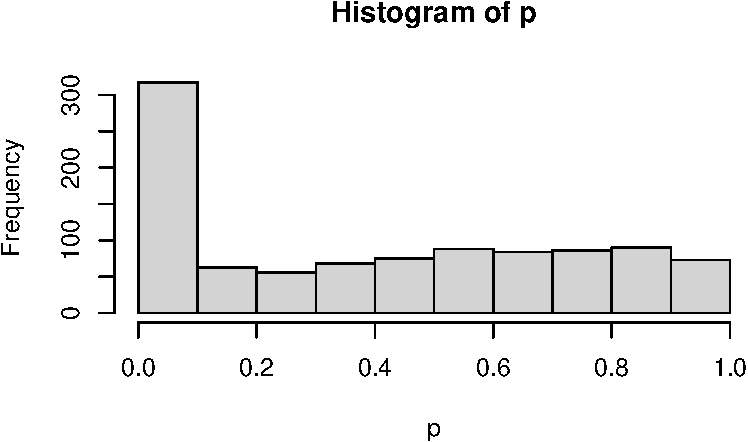
\includegraphics[keepaspectratio]{chapter10_files/figure-pdf/unnamed-chunk-6-1.pdf}}

\begin{Shaded}
\begin{Highlighting}[]
\FunctionTok{hist}\NormalTok{(add.vec)}
\end{Highlighting}
\end{Shaded}

\pandocbounded{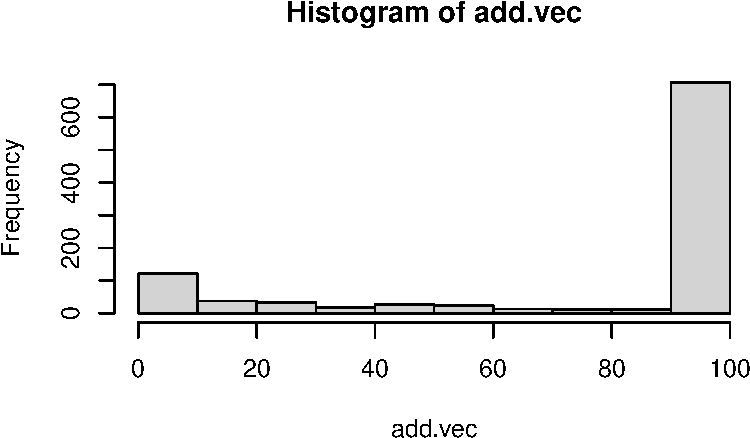
\includegraphics[keepaspectratio]{chapter10_files/figure-pdf/unnamed-chunk-6-2.pdf}}

結果をみると,0.306とかなり逸脱して,誤った結論に辿り着いていることがわかる。努力の結果得られた有意差は,偶然の賜物でもあり,誤った研究実践による幻想にすぎない。加えたデータのヒストグラムからわかるように,悲しいかな,75\%もの割合で上限100まで達してしまう。百害あって一利なしとはこのことである。

\subsection{サンプルサイズを事前に決めないことの問題}\label{ux30b5ux30f3ux30d7ux30ebux30b5ux30a4ux30baux3092ux4e8bux524dux306bux6c7aux3081ux306aux3044ux3053ux3068ux306eux554fux984c}

サンプルサイズを事前に決めずに検定する,という状況を別の角度から見てみよう。\textcite{Maeda2017}
は「コインフリップを24回して,うち7回表が出た」というシーンを例に挙げて説明している。7/24は半分を下回っているから,やや裏が出やすいコインであるように思える。帰無仮説として,このコインは公平である(表と裏が出る確率が半々である),というのを検証したいとする。

この24回中7回成功,という話の背後に「24施行する」ということを決めていたかどうか(サンプルサイズを事前に決めていたか)ということを考えてみよう。

まずは正直に,最初から24回コインフリップすることを決めていたとする。コインフリップはベルヌーイ試行\footnote{表(1)が出るか,裏(0)が出るか,という2値の結果変数だけを持つ施行のことで,この確率変数がベルヌーイ分布にし違う。ベルヌーイ分布は,表が出る確率\(\theta\)をパラメータに持つ。\(P(X=k) = \theta^k(1-\theta)^{1-k},\text{ただし}k=\{0,1\}\)という確率変数である。1/0というのが生死,男女,成功失敗などさまざまなメタファに適用できるので応用範囲が広い。}
であり,それを繰り返すので二項分布に従うと考えられる。そこで,二項検定として次のように計算できるだろう。

\begin{Shaded}
\begin{Highlighting}[]
\NormalTok{N }\OtherTok{\textless{}{-}} \DecValTok{24}
\CommentTok{\# 7回表が出る確率}
\FunctionTok{pbinom}\NormalTok{(}\DecValTok{7}\NormalTok{, N, }\FloatTok{0.5}\NormalTok{) }\SpecialCharTok{*} \DecValTok{2}
\end{Highlighting}
\end{Shaded}

\begin{verbatim}
[1] 0.06391466
\end{verbatim}

二項分布のp値を出すには\texttt{pbinom}を使いった。また帰無仮説として,このコインフリップは公平であると考えているのだから,\(\theta=0.5\)が帰無仮説の状態である。この\(\theta=0.5\)とした時に,\(N=24,k=7\)という結果になる確率を計算し,かつ両側検定(公平でない,が対立仮説なので裏が7回でもよい)であることを考えて確率を2倍した。p値は0.0639147であるから,5\%水準では有意であると判定できない。これぐらいの確率はあるということだ。

しかしここで第二の状況を考えてみよう。24回コインフリップすることを決めていたのではなくて,7回成功するまでコインフリップを続けたところ,結果的に24回で終わったということだった,とするのである。このようなシーンの確率分布は負の二項分布と呼ばれ,\texttt{pnbinom}で次のように計算できる。

\begin{Shaded}
\begin{Highlighting}[]
\NormalTok{k }\OtherTok{\textless{}{-}} \DecValTok{7}
\CommentTok{\# 24回以上必要な確率}
\FunctionTok{pnbinom}\NormalTok{(k, }\DecValTok{24}\NormalTok{, }\FloatTok{0.5}\NormalTok{) }\SpecialCharTok{*} \DecValTok{2}
\end{Highlighting}
\end{Shaded}

\begin{verbatim}
[1] 0.003326893
\end{verbatim}

この結果から,\(\theta=0.5\)の時に7回表がでるまでに24施行も必要とする確率は,0.0033269だから,5\%水準で有意である。つまり,滅多にこんなことが起きないので,\(\theta=0.5\)という帰無仮説が疑わしいことになる。ここではシーンが異なるとp値が違っている,ということに注意してほしい。

さらに第3のシーンを考えよう。これは「何回やるかは決めてないけど,まあ5分ぐらいかな」と試行にかける時間だけ決めていたという状況である。結果的に24回になったけど,もしかすると23回だったかもしれないし,25回や20回,30回だったかもしれない。これをシミュレーションするために,「24がピークになるような頻度の分布」をポアソン分布を使って生成する\footnote{もちろん基準となる有意水準\(\alpha\),検出力\(1-\beta\)も定める必要があるが,慣例的に\(\alpha = 0.05\)であり,\(1-\beta =0.8\)ぐらいが必要とされている。}。

\footnote{もちろん基準となる有意水準\(\alpha\),検出力\(1-\beta\)も定める必要があるが,慣例的に\(\alpha = 0.05\)であり,\(1-\beta =0.8\)ぐらいが必要とされている。}
ポアソン分布は正の整数を実現値に取る分布で,カウント変数の確率分布として用いられる。パラメータは\(\lambda\)だけであり,期待値と分散が\(\lambda\)に一致する,非常にシンプルな分布である。

\begin{Shaded}
\begin{Highlighting}[]
\FunctionTok{set.seed}\NormalTok{(}\DecValTok{12345}\NormalTok{)}
\NormalTok{iter }\OtherTok{\textless{}{-}} \DecValTok{100000} \CommentTok{\# 発生させる乱数の数}
\DocumentationTok{\#\# 24回がピークに来るトライアル回数}
\NormalTok{trial }\OtherTok{\textless{}{-}} \FunctionTok{rpois}\NormalTok{(iter, }\DecValTok{24}\NormalTok{)}
\FunctionTok{hist}\NormalTok{(trial)}
\end{Highlighting}
\end{Shaded}

\pandocbounded{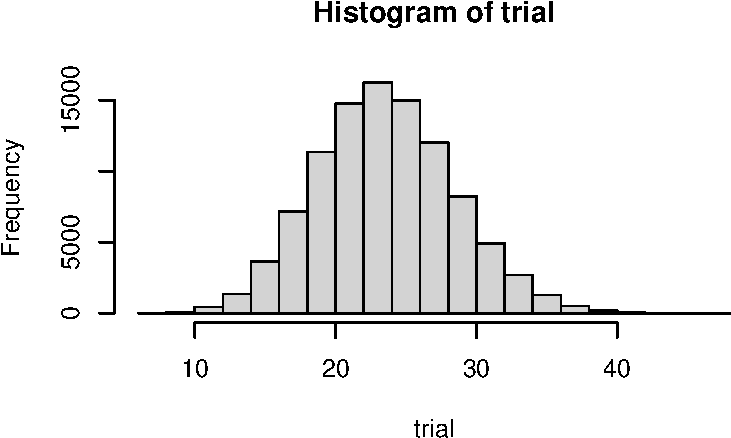
\includegraphics[keepaspectratio]{chapter10_files/figure-pdf/unnamed-chunk-9-1.pdf}}

この各トライアルにおいて,二項分布で成功した回数を計算し,トライアル回数で割ることによって,表が出る確率のシミュレーションができる。その時の割合は,\(7/24\)よりもレアな現象だろうか?

\begin{Shaded}
\begin{Highlighting}[]
\NormalTok{result }\OtherTok{\textless{}{-}} \FunctionTok{rep}\NormalTok{(}\ConstantTok{NA}\NormalTok{, iter)}
\ControlFlowTok{for}\NormalTok{ (i }\ControlFlowTok{in} \DecValTok{1}\SpecialCharTok{:}\NormalTok{iter) \{}
\NormalTok{  result[i] }\OtherTok{\textless{}{-}} \FunctionTok{rbinom}\NormalTok{(}\DecValTok{1}\NormalTok{, trial[i], }\FloatTok{0.5}\NormalTok{) }\SpecialCharTok{/}\NormalTok{ trial[i]}
\NormalTok{\}}
\DocumentationTok{\#\# 7/24よりも小さい確率で起こった?}
\FunctionTok{length}\NormalTok{(result[result }\SpecialCharTok{\textless{}}\NormalTok{ (}\DecValTok{7} \SpecialCharTok{/} \DecValTok{24}\NormalTok{)]) }\SpecialCharTok{/}\NormalTok{ iter}
\end{Highlighting}
\end{Shaded}

\begin{verbatim}
[1] 0.02262
\end{verbatim}

これを見ると,両側検定にしても0.04524なので,ギリギリ有意になるかどうか,というところだろうか。

さて判断にこまった。「24回やる」と決めていたのであれば\(\theta=0.5\)は棄却されないし,「7回成功するまで」と決めていたのであれば\(\theta=0.5\)は棄却される。「5分間」と決めていても棄却されるが,そもそもこうした実験者の意図によって判断が揺らいで良いものだろうか?というのが
\textcite{Maeda2017} の指摘する疑問点である。

問題は,「24回中7回成功」という事実に,二項分布,負の二項分布,あるいは組み合わさった分布のような,確率分布の情報が含まれていないことにある。この確率分布はデータが既知で母数が未知だから尤度関数であり,データ生成メカニズムであるとも言えるだろう。想定するメカニズムが明示されない検定は,ともすれば事後的に「実は負の二項分布を想定していたんですよ,へへ」ということも可能になってしまう。こうした点からも,研究者の自由度をなるべく少なくする研究計画の\textbf{事前登録}制度が必要であることがわかる。

\section{サンプルサイズ設計}\label{ux30b5ux30f3ux30d7ux30ebux30b5ux30a4ux30baux8a2dux8a08}

どのようにデータを取り,どのように分析・検定し,どのような基準で判断するかを事前に決めることに加え,事前にサンプルサイズを見積もっておく必要があるだろう。サンプルはとにかく多ければ多いほど良いか,というとそうではなく,過剰にサンプルを集めることは研究コストの増大であり,回答者の負担増でしかない。またサンプルサイズが大きくなると有意差を検出しやすくなるが,必要なのは有意差ではなく実質的に効果を見積もることであり,有意差が見つかれば良いというものではないことに注意が必要である。もちろん上で見てきたように,有意差が検出できるかどうかを指標にしてサンプルサイズを変動させてしまうのは,明らかに誤った研究実践である。

事前にサンプルサイズを決定するのに必要なのは,これまでのリバースエンジニアリングの演習例からもわかるように,効果量の見積もりである。\footnote{もちろん基準となる有意水準\(\alpha\),検出力\(1-\beta\)も定める必要があるが,慣例的に\(\alpha = 0.05\)であり,\(1-\beta =0.8\)ぐらいが必要とされている。}
これをどのように定めるかについては,先行研究を考えるとか,研究領域で「これぐらい差がないと意味がないよね」とコンセンサスが取れている程度で決めることになる。\footnote{この「最低限検出したい効果」のことをSmallest
  Effect Size of Interest, SESOIと呼ぶ。\textcite{kosugi2023} も参照。}

\subsection{対応のないt検定}\label{ux5bfeux5fdcux306eux306aux3044tux691cux5b9a}

サンプルサイズの設計には,これまで使ってきた検定統計量に\textbf{非心度}non-centrality
parameterというパラメータを加えて考える必要がある。

具体的に,対応のないt検定を例にサンプルサイズ設計の方法を見てみよう。t検定は言葉の通り,t分布を用いて帰無仮説の元での検定統計量の実現値が問題になるのであった。帰無仮説は\(\mu_0 = \mu_1-\mu_2 = 0\)であり,検定統計量は次式で表されるのであった。

\[ T = \frac{d - \mu_0}{\sqrt{U^2_p/\frac{n_1n_2}{n_1+n_2}}}\]

この分子において,\(d - \mu_0 = (\bar{X}_1 - \bar{X}_2) - (\mu_1 - \mu_2)\)の第二項を,\(\mu_1-\mu_2 = 0\)と仮定するから,\(0\)が中心の標準化されたt分布が用いられたのである。帰無仮説はこのように理論的に特定できる比較点をもとに置かれているのであって,帰無仮説下ではない現実の世界では,検定統計量は母平均の差\(\mu_1 - \mu_2\)に応じた分布から生じている。このように中心がずれているt分布のことを\textbf{非心分布}といい,ズレの程度が非心度パラメータである。t検定における非心度\(\lambda\)は,以下の式で表される。

\[ \lambda = \frac{(\mu_1-\mu2) - \mu_0}{\sigma\sqrt{n}} \]

この非心度の分だけ,非心t分布はt分布からズレていることになる。Rでは\texttt{dt}関数に\texttt{ncp}パラメータがあり,デフォルトでは\texttt{ncp=0}になっていた。これを変えて描画してみよう。

\begin{Shaded}
\begin{Highlighting}[]
\CommentTok{\# データの準備}
\NormalTok{df }\OtherTok{\textless{}{-}} \DecValTok{10} \CommentTok{\# 自由度を指定}
\CommentTok{\# ggplotでプロット}
\FunctionTok{ggplot}\NormalTok{(}\FunctionTok{data.frame}\NormalTok{(}\AttributeTok{x =} \FunctionTok{c}\NormalTok{(}\SpecialCharTok{{-}}\DecValTok{5}\NormalTok{, }\DecValTok{5}\NormalTok{)), }\FunctionTok{aes}\NormalTok{(}\AttributeTok{x =}\NormalTok{ x)) }\SpecialCharTok{+}
  \FunctionTok{stat\_function}\NormalTok{(}\AttributeTok{fun =}\NormalTok{ dt, }\AttributeTok{args =} \FunctionTok{list}\NormalTok{(}\AttributeTok{df =}\NormalTok{ df, }\AttributeTok{ncp =} \DecValTok{0}\NormalTok{), }\FunctionTok{aes}\NormalTok{(}\AttributeTok{color =} \StringTok{"ncp=0"}\NormalTok{)) }\SpecialCharTok{+}
  \FunctionTok{stat\_function}\NormalTok{(}\AttributeTok{fun =}\NormalTok{ dt, }\AttributeTok{args =} \FunctionTok{list}\NormalTok{(}\AttributeTok{df =}\NormalTok{ df, }\AttributeTok{ncp =} \DecValTok{3}\NormalTok{), }\FunctionTok{aes}\NormalTok{(}\AttributeTok{color =} \StringTok{"ncp=3"}\NormalTok{)) }\SpecialCharTok{+}
  \FunctionTok{labs}\NormalTok{(}
    \AttributeTok{title =} \StringTok{"非心t分布"}\NormalTok{,}
    \AttributeTok{x =} \StringTok{"x"}\NormalTok{,}
    \AttributeTok{y =} \StringTok{"密度"}\NormalTok{,}
    \AttributeTok{color =} \StringTok{"ncp"}
\NormalTok{  )}
\end{Highlighting}
\end{Shaded}

\pandocbounded{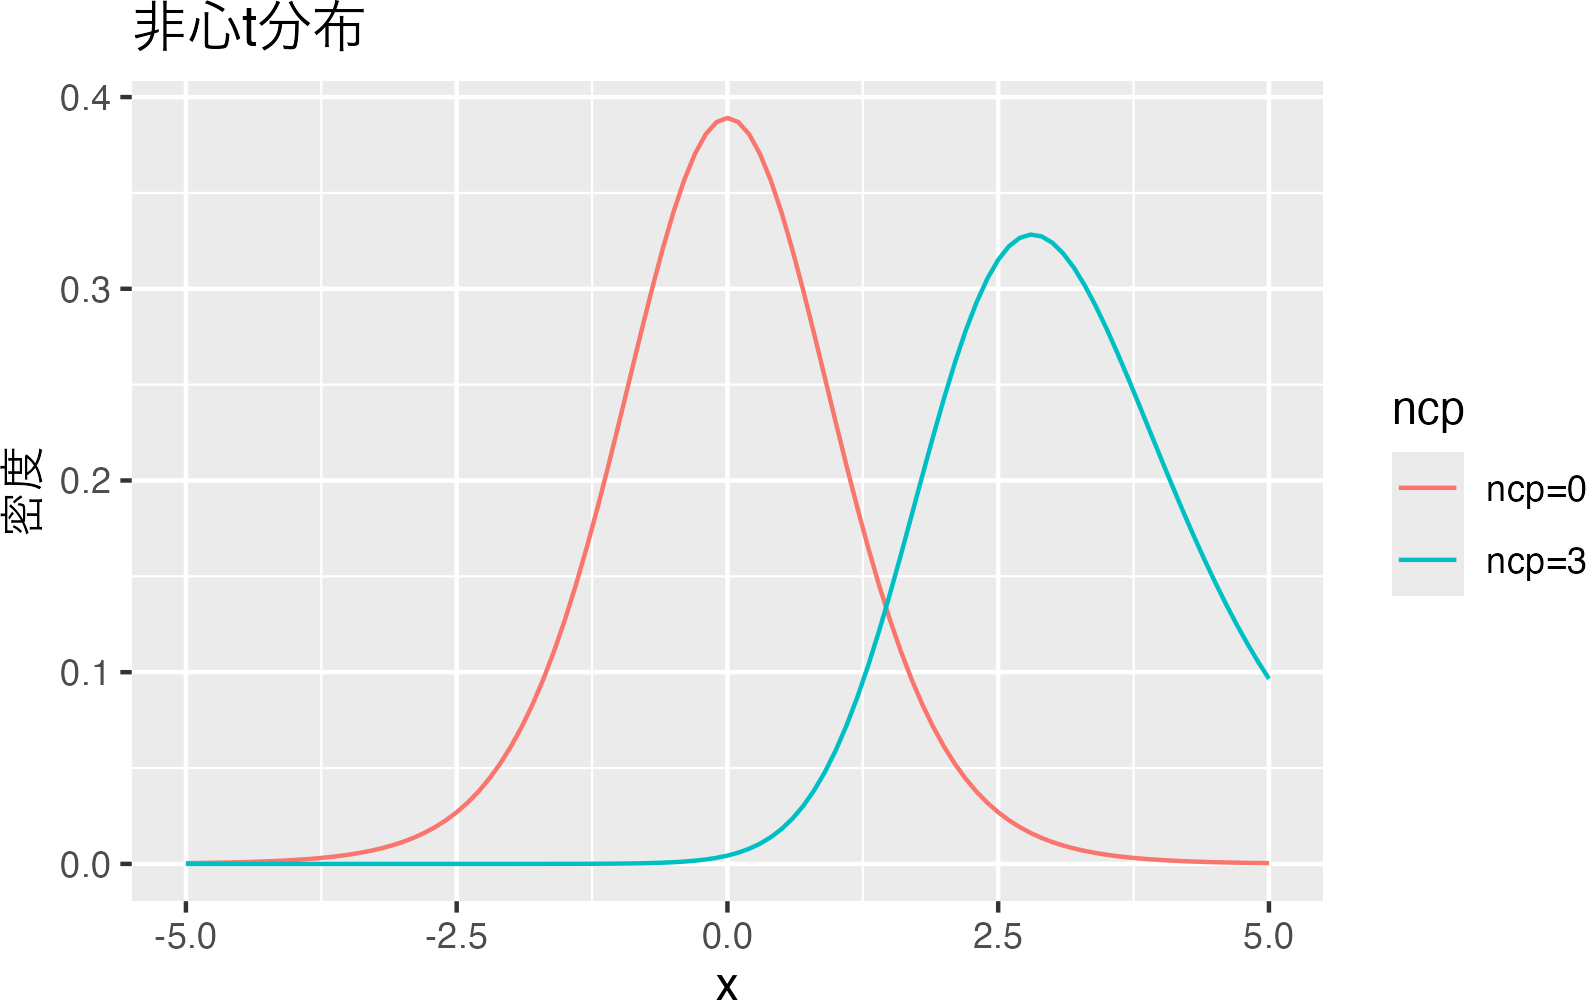
\includegraphics[keepaspectratio]{chapter10_files/figure-pdf/unnamed-chunk-11-1.png}}

\texttt{ncp=0}の時は,中心が\texttt{0}にある帰無仮説の世界であり,これを使ってタイプ1エラー,つまり\(\alpha\)が算出されたのであった。\texttt{ncp}を効果量で表現すれば,母平均の差がゼロでない時の分布が描けるのだから,タイプ2エラー,つまり\(\beta\)が計算できる。

自由度\texttt{df\ =\ 10},非心度\texttt{ncp\ =\ 3}の例で考えてみよう。
タイプ1エラーになるのは,自由度\texttt{10}のt分布で上2.5\%の臨界値以上の実現値が得られた時である。

\begin{Shaded}
\begin{Highlighting}[]
\FunctionTok{qt}\NormalTok{(}\FloatTok{0.975}\NormalTok{, }\AttributeTok{df =} \DecValTok{10}\NormalTok{, }\AttributeTok{ncp =} \DecValTok{0}\NormalTok{)}
\end{Highlighting}
\end{Shaded}

\begin{verbatim}
[1] 2.228139
\end{verbatim}

このとき,実際は\texttt{ncp\ =\ 3}ほどずれていたのだから,タイプ2エラーが生じる確率は次のとおりである。

\begin{Shaded}
\begin{Highlighting}[]
\FunctionTok{qt}\NormalTok{(}\FloatTok{0.975}\NormalTok{, }\AttributeTok{df =} \DecValTok{10}\NormalTok{, }\AttributeTok{ncp =} \DecValTok{0}\NormalTok{) }\SpecialCharTok{\%\textgreater{}\%} \FunctionTok{pt}\NormalTok{(}\AttributeTok{df =} \DecValTok{10}\NormalTok{, }\AttributeTok{ncp =} \DecValTok{3}\NormalTok{)}
\end{Highlighting}
\end{Shaded}

\begin{verbatim}
[1] 0.2285998
\end{verbatim}

当然,\texttt{ncp\ =\ 0}から離れるほどタイプ2エラーは生じにくくなる。非心度は母効果量\(\delta = \frac{(\mu_1 - \mu_2)-\mu_0}{\delta}\)を使って,\(\lambda = \delta \sqrt{n}\)で表すことができる。

これを使って,t検定のサンプルサイズを設計してみよう。話を簡単にするために,サンプルサイズは2群で等しいものとする。

検定統計量の式を思い出して,\(\sqrt{n}\)にあたるところは2群のサンプルサイズから計算される,プールされた標本サイズから得られることに注意しよう\footnote{t統計量の実現値の式にある分母,\(\sqrt{U_p^2/\frac{n_1n_2}{n_1+n_2}}\)に見られる,プールされた不偏分散を割るための標本サイズであり,2群の母分散が等しいと仮定して計算するなら,\(\sigma^2(\frac{1}{n_1} + \frac{1}{n_2}) = \sigma^2(\frac{n_1+n_2}{n_1n_2}) = \sigma^2 / \frac{n_1n_2}{n_1 + n_2}\)から得られる。}。

\begin{Shaded}
\begin{Highlighting}[]
\NormalTok{alpha }\OtherTok{\textless{}{-}} \FloatTok{0.05}
\NormalTok{beta }\OtherTok{\textless{}{-}} \FloatTok{0.2}
\NormalTok{delta }\OtherTok{\textless{}{-}} \FloatTok{0.5}

\ControlFlowTok{for}\NormalTok{ (n }\ControlFlowTok{in} \DecValTok{10}\SpecialCharTok{:}\DecValTok{1000}\NormalTok{) \{}
\NormalTok{  df }\OtherTok{\textless{}{-}}\NormalTok{ n }\SpecialCharTok{+}\NormalTok{ n }\SpecialCharTok{{-}} \DecValTok{2}
\NormalTok{  lambda }\OtherTok{\textless{}{-}}\NormalTok{ delta }\SpecialCharTok{*}\NormalTok{ (}\FunctionTok{sqrt}\NormalTok{((n }\SpecialCharTok{*}\NormalTok{ n) }\SpecialCharTok{/}\NormalTok{ (n }\SpecialCharTok{+}\NormalTok{ n)))}
\NormalTok{  cv }\OtherTok{\textless{}{-}} \FunctionTok{qt}\NormalTok{(}\AttributeTok{p =} \DecValTok{1} \SpecialCharTok{{-}}\NormalTok{ alpha }\SpecialCharTok{/} \DecValTok{2}\NormalTok{, }\AttributeTok{df =}\NormalTok{ df) }\CommentTok{\# Type1errorの臨界値}
\NormalTok{  er }\OtherTok{\textless{}{-}} \FunctionTok{pt}\NormalTok{(cv, }\AttributeTok{df =}\NormalTok{ df, }\AttributeTok{ncp =}\NormalTok{ lambda) }\CommentTok{\# Type2errorの確率}
  \ControlFlowTok{if}\NormalTok{ (er }\SpecialCharTok{\textless{}=}\NormalTok{ beta) \{}
    \ControlFlowTok{break}
\NormalTok{  \}}
\NormalTok{\}}
\FunctionTok{print}\NormalTok{(n)}
\end{Highlighting}
\end{Shaded}

\begin{verbatim}
[1] 64
\end{verbatim}

ここでは,サンプルサイズを10から徐々に増やしていき,1000までの間で目標とする\(\beta\)まで抑えられたところで,カウントしていく\texttt{for}ループを\texttt{break}で脱出する,というかたちで組んでいる。結果的に,各群64名,合計128名のサンプルがあれば,目標が達成できることがわかる。サンプルサイズが2群で異なる場合など,詳細は@kosugi2023
に詳しい。

\subsection{シミュレーションによるサンプルサイズ設計}\label{ux30b7ux30dfux30e5ux30ecux30fcux30b7ux30e7ux30f3ux306bux3088ux308bux30b5ux30f3ux30d7ux30ebux30b5ux30a4ux30baux8a2dux8a08}

非心F分布を使えば分散分析でもサンプルサイズができるし,そのほかの検定についても同様に非心分布を活用すると良い。しかし,非心分布の理解や非心度の計算など,ケースバイケースで学ぶべきことは多い。

そこで,電子計算機の演算力をたのみに,データ生成のシミュレーションを通じて設計していくことを考えてみよう。サンプルサイズや効果量を定めれば,仮想データを作ることができるし,それ対して検定をかけることもできる。仮想データの生成と検定を反復し,タイプ2エラーがどの程度生じるかを相対度数で近似することもできるだろう。であれば,その近似をサンプルサイズを徐々に変えることで繰り返してサンプルサイズを定めることもできる。

以下は,母相関が\(\rho = 0.5\)とした時に,検出力が80\%になるために必要なサンプルサイズを求めるシミュレーションコードである。

\begin{Shaded}
\begin{Highlighting}[]
\NormalTok{pacman}\SpecialCharTok{::}\FunctionTok{p\_load}\NormalTok{(MASS)}
\FunctionTok{set.seed}\NormalTok{(}\DecValTok{12345}\NormalTok{)}
\NormalTok{alpha }\OtherTok{\textless{}{-}} \FloatTok{0.05}
\NormalTok{beta }\OtherTok{\textless{}{-}} \FloatTok{0.2}
\NormalTok{rho }\OtherTok{\textless{}{-}} \FloatTok{0.5}
\NormalTok{sd }\OtherTok{\textless{}{-}} \DecValTok{1}
\NormalTok{Sigma }\OtherTok{\textless{}{-}} \FunctionTok{matrix}\NormalTok{(}\ConstantTok{NA}\NormalTok{, }\AttributeTok{ncol =} \DecValTok{2}\NormalTok{, }\AttributeTok{nrow =} \DecValTok{2}\NormalTok{)}
\NormalTok{Sigma[}\DecValTok{1}\NormalTok{, }\DecValTok{1}\NormalTok{] }\OtherTok{\textless{}{-}}\NormalTok{ Sigma[}\DecValTok{2}\NormalTok{, }\DecValTok{2}\NormalTok{] }\OtherTok{\textless{}{-}}\NormalTok{ sd}\SpecialCharTok{\^{}}\DecValTok{2}
\NormalTok{Sigma[}\DecValTok{1}\NormalTok{, }\DecValTok{2}\NormalTok{] }\OtherTok{\textless{}{-}}\NormalTok{ Sigma[}\DecValTok{2}\NormalTok{, }\DecValTok{1}\NormalTok{] }\OtherTok{\textless{}{-}}\NormalTok{ sd }\SpecialCharTok{*}\NormalTok{ sd }\SpecialCharTok{*}\NormalTok{ rho}

\NormalTok{iter }\OtherTok{\textless{}{-}} \DecValTok{1000}

\ControlFlowTok{for}\NormalTok{ (n }\ControlFlowTok{in} \FunctionTok{seq}\NormalTok{(}\AttributeTok{from =} \DecValTok{10}\NormalTok{, }\AttributeTok{to =} \DecValTok{1000}\NormalTok{, }\AttributeTok{by =} \DecValTok{1}\NormalTok{)) \{}
\NormalTok{  FLG }\OtherTok{\textless{}{-}} \FunctionTok{rep}\NormalTok{(}\DecValTok{0}\NormalTok{, iter)}
  \ControlFlowTok{for}\NormalTok{ (i }\ControlFlowTok{in} \DecValTok{1}\SpecialCharTok{:}\NormalTok{iter) \{}
\NormalTok{    X }\OtherTok{\textless{}{-}} \FunctionTok{mvrnorm}\NormalTok{(n, }\FunctionTok{c}\NormalTok{(}\DecValTok{0}\NormalTok{, }\DecValTok{0}\NormalTok{), Sigma)}
\NormalTok{    cor\_test }\OtherTok{\textless{}{-}} \FunctionTok{cor.test}\NormalTok{(X[, }\DecValTok{1}\NormalTok{], X[, }\DecValTok{2}\NormalTok{])}
\NormalTok{    FLG[i] }\OtherTok{\textless{}{-}} \FunctionTok{ifelse}\NormalTok{(cor\_test}\SpecialCharTok{$}\NormalTok{p.value }\SpecialCharTok{\textgreater{}}\NormalTok{ alpha, }\DecValTok{1}\NormalTok{, }\DecValTok{0}\NormalTok{)}
\NormalTok{  \}}
\NormalTok{  t2error }\OtherTok{\textless{}{-}} \FunctionTok{mean}\NormalTok{(FLG)}
  \FunctionTok{print}\NormalTok{(}\FunctionTok{paste}\NormalTok{(}\StringTok{"n="}\NormalTok{, n, }\StringTok{"のとき,betaは"}\NormalTok{, t2error, }\StringTok{"です。"}\NormalTok{))}
  \ControlFlowTok{if}\NormalTok{ (t2error }\SpecialCharTok{\textless{}=}\NormalTok{ beta) \{}
    \ControlFlowTok{break}
\NormalTok{  \}}
\NormalTok{\}}
\end{Highlighting}
\end{Shaded}

\begin{verbatim}
[1] "n= 10 のとき,betaは 0.681 です。"
[1] "n= 11 のとき,betaは 0.639 です。"
[1] "n= 12 のとき,betaは 0.612 です。"
[1] "n= 13 のとき,betaは 0.566 です。"
[1] "n= 14 のとき,betaは 0.563 です。"
[1] "n= 15 のとき,betaは 0.471 です。"
[1] "n= 16 のとき,betaは 0.462 です。"
[1] "n= 17 のとき,betaは 0.419 です。"
[1] "n= 18 のとき,betaは 0.402 です。"
[1] "n= 19 のとき,betaは 0.385 です。"
[1] "n= 20 のとき,betaは 0.353 です。"
[1] "n= 21 のとき,betaは 0.344 です。"
[1] "n= 22 のとき,betaは 0.312 です。"
[1] "n= 23 のとき,betaは 0.285 です。"
[1] "n= 24 のとき,betaは 0.256 です。"
[1] "n= 25 のとき,betaは 0.265 です。"
[1] "n= 26 のとき,betaは 0.21 です。"
[1] "n= 27 のとき,betaは 0.227 です。"
[1] "n= 28 のとき,betaは 0.176 です。"
\end{verbatim}

\begin{Shaded}
\begin{Highlighting}[]
\FunctionTok{print}\NormalTok{(n)}
\end{Highlighting}
\end{Shaded}

\begin{verbatim}
[1] 28
\end{verbatim}

ここではシミュレーション回数1000,上限1000,刻み幅を1にしているが,状況に応じて変更すると良い。

\section{課題}\label{ux8ab2ux984c-8}

\begin{enumerate}
\def\labelenumi{\arabic{enumi}.}
\tightlist
\item
  一要因3水準のBetweenデザインの分散分析において、1.分散分析で有意差が見られる場合と、2.任意の2水準の組み合わせのどこかで有意差が見られる場合を考えたとき、タイプ1エラーはどのように異なるかをシミュレーションで確かめてみましょう。設定として、\texttt{n1=n2=n3=10}、標準偏差も各群等しく\texttt{sigma\ =\ 1}としてみましょう。
\item
  N増し問題は相関係数の検定の時も生じるでしょうか。母相関が\(\rho = 0.0\)のとき、サンプルサイズを10から始めて、有意になるまでデータを追加する仮想研究を1000回行ってみましょう。データ追加の上限は100、有意水準は\(\alpha = 0.05\)として、最終的に有意になる割合を計算してみましょう。
\item
  \(\alpha = 0.05, \beta = 0.2\)とし、効果量\(\delta = 1\)とした時の対応のないt検定のサンプルサイズ設計をしたいです。1.非心t分布を使った解析的な方法と、2.シミュレーションによる近似的な方法の両方で、同等の結果が出ることを確認しましょう。
\end{enumerate}

\bookmarksetup{startatroot}

\chapter{重回帰分析の基礎}\label{ux91cdux56deux5e30ux5206ux6790ux306eux57faux790e}

\section{回帰分析の基礎}\label{ux56deux5e30ux5206ux6790ux306eux57faux790e}

ここでは回帰分析を扱う。説明変数\(x\)と被説明変数\(y\)の関数関係\(y=f(x)\)に,次の一次式を当てはめるのが単回帰分析である。

\[ y_i  = \beta_0 + \beta_1 x_i + e_i = \hat{y}_i + e_i\]

一次式を\(\hat{y}\)とまとめたものを予測値といい,予測値と実測値\(y\)の差分\(e_i\)を残差residualsという。

空間上の一次直線の切片,傾きを求めるというのが基本的な問題であり,二点であれば一意に定めることができるが,データ分析の場面では3点以上の多くのデータセットの中に直線を当てはめることになるので,なんらかの外的な基準が必要になる。この時,「残差の分散が最も小さくなるように」と考えるのが\textbf{最小二乗法}の考え方であり,「残差が正規分布に従っていると考え,その尤度が最も大きくなるように」と考えるのが\textbf{最尤法}の考え方である。前者は記述統計的な,後者は確率モデルとしての感が過多になっていることに注意してほしい。また確率モデルの推定方法としては,事前分布を用いた\textbf{ベイズ推定}が用いられることもある。

最小二乗法による推定値は,次の式で表される。証明は他書\autocite{kosugi2018,Nishiuchi201712}に譲るが,ロジックとして残差の二乗和\(\sum e_i^2 = \sum (y_i - (\beta_0 + \beta_1 x_i))^2\)を最小にすることを考え,この式を展開するか偏微分を用いて極小値を求めることで算出できるとだけ伝えておこう。いずれにせよ,平均値\(\bar{x},\bar{y}\)や分散・共分散\(s_x,s_y,r_{xy}\)など標本統計量から推定できるのはありがたいことである。

\[\beta_0 = \bar{y} - \beta_1\bar{x},\quad \beta_1 = r_{xy} \frac{s_y}{s_x}\]

また,ここでは\(x,y\)ともに連続変数を想定しているが,説明変数\(x\)が二値,あるいはカテゴリカルなものであれば\(y\)の平均値を通る直線を探すことになる。直線の傾きが0であれば「平均値が同じ」という線形モデルであり,これは平均値差の検定における帰無仮説と同等である。このように,t検定やANOVAは回帰分析の特殊ケースとも考えられ,まとめて\textbf{一般線形モデル}と呼ばれる。一般線形モデルは,被説明変数が連続的で,線形モデルによる平均値に正規分布に従う残差が加わったものとして考えるという意味で統一的に表現される。

ANOVAの場合は,二つ以上の要因による効果を考えることもあった。交互作用項を考慮しなければ,2要因のモデルは次のように表現することができる。

\[ y_i = \beta_0 + \beta_1 x_{1i} + \beta_2 x_{2i} + e_i \]

このように説明変数が複数ある回帰分析を特に重回帰分析Multiple Regression
Analysisと呼ぶ。一次式なので,ある変数に限れば線形性が担保されているから,これも線形モデルの仲間である。重回帰分析を用いる場合は,説明変数同士を比較して「どちらの説明変数の方が影響力が大きいか」ということが論じられることが多いが,係数は当然\(x_n, y\)の単位に依存するため,素点の回帰係数は使い勝手が悪い。そこですべての変数を標準化した標準化係数が用いられることが多い。

\section{回帰分析の特徴}\label{ux56deux5e30ux5206ux6790ux306eux7279ux5fb4}

以下,具体的なデータを用いて回帰分析の特徴を見てみよう

\subsection{パラメータリカバリ}\label{ux30d1ux30e9ux30e1ux30fcux30bfux30eaux30abux30d0ux30ea}

回帰分析のモデル式にそってデータを生成し,分析によってパラメータリカバリを行ってみよう。

説明変数については制約がないので一様乱数から生成し,平均0,標準偏差\(\sigma\)の誤差とともに被説明変数を作る。

\begin{Shaded}
\begin{Highlighting}[]
\NormalTok{pacman}\SpecialCharTok{::}\FunctionTok{p\_load}\NormalTok{(tidyverse)}
\FunctionTok{set.seed}\NormalTok{(}\DecValTok{123}\NormalTok{)}
\NormalTok{n }\OtherTok{\textless{}{-}} \DecValTok{500}
\NormalTok{beta0 }\OtherTok{\textless{}{-}} \DecValTok{2}
\NormalTok{beta1 }\OtherTok{\textless{}{-}} \DecValTok{3}
\NormalTok{sigma }\OtherTok{\textless{}{-}} \DecValTok{1}
\CommentTok{\# データの生成}
\NormalTok{x }\OtherTok{\textless{}{-}} \FunctionTok{runif}\NormalTok{(n, }\SpecialCharTok{{-}}\DecValTok{10}\NormalTok{, }\DecValTok{10}\NormalTok{)}
\NormalTok{e }\OtherTok{\textless{}{-}} \FunctionTok{rnorm}\NormalTok{(n, }\DecValTok{0}\NormalTok{, sigma)}
\NormalTok{y }\OtherTok{\textless{}{-}}\NormalTok{ beta0 }\SpecialCharTok{+}\NormalTok{ beta1 }\SpecialCharTok{*}\NormalTok{ x }\SpecialCharTok{+}\NormalTok{ e}

\NormalTok{dat }\OtherTok{\textless{}{-}} \FunctionTok{data.frame}\NormalTok{(x, y)}
\CommentTok{\# データの確認}
\FunctionTok{head}\NormalTok{(dat)}
\end{Highlighting}
\end{Shaded}

\begin{verbatim}
          x          y
1 -4.248450 -11.120952
2  5.766103  18.736432
3 -1.820462  -3.805302
4  7.660348  25.071541
5  8.809346  30.026546
6 -9.088870 -25.355175
\end{verbatim}

\begin{Shaded}
\begin{Highlighting}[]
\NormalTok{dat }\SpecialCharTok{\%\textgreater{}\%} \FunctionTok{ggplot}\NormalTok{(}\FunctionTok{aes}\NormalTok{(}\AttributeTok{x =}\NormalTok{ x, }\AttributeTok{y =}\NormalTok{ y)) }\SpecialCharTok{+}
  \FunctionTok{geom\_point}\NormalTok{() }\SpecialCharTok{+}
  \FunctionTok{geom\_smooth}\NormalTok{(}\AttributeTok{method =} \StringTok{"lm"}\NormalTok{, }\AttributeTok{formula =} \StringTok{"y\textasciitilde{}x"}\NormalTok{) }\CommentTok{\# 線形モデルの描画}
\end{Highlighting}
\end{Shaded}

\pandocbounded{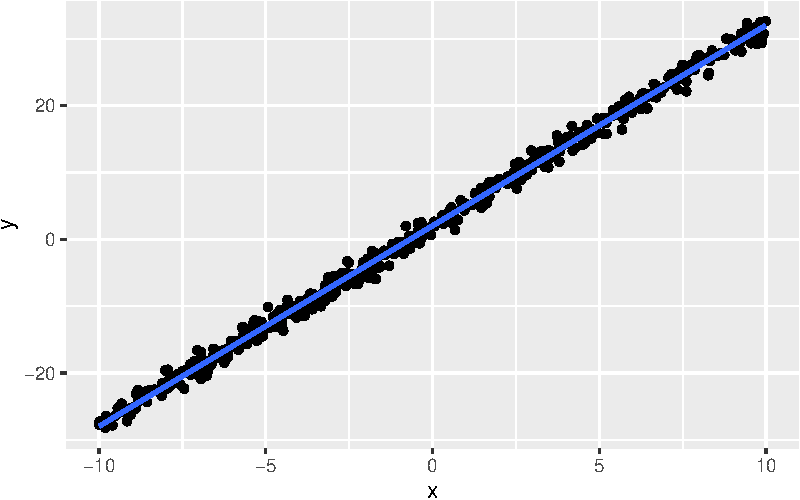
\includegraphics[keepaspectratio]{chapter11_files/figure-pdf/unnamed-chunk-1-1.pdf}}

このデータに基づいて回帰分析を実行した結果が以下のとおりである。

\begin{Shaded}
\begin{Highlighting}[]
\NormalTok{result.lm }\OtherTok{\textless{}{-}} \FunctionTok{lm}\NormalTok{(y }\SpecialCharTok{\textasciitilde{}}\NormalTok{ x, }\AttributeTok{data =}\NormalTok{ dat)}
\FunctionTok{summary}\NormalTok{(result.lm)}
\end{Highlighting}
\end{Shaded}

\begin{verbatim}

Call:
lm(formula = y ~ x, data = dat)

Residuals:
     Min       1Q   Median       3Q      Max 
-2.82796 -0.61831  0.03553  0.69367  2.68062 

Coefficients:
            Estimate Std. Error t value Pr(>|t|)    
(Intercept) 2.021928   0.045010   44.92   <2e-16 ***
x           3.002194   0.007919  379.09   <2e-16 ***
---
Signif. codes:  0 '***' 0.001 '**' 0.01 '*' 0.05 '.' 0.1 ' ' 1

Residual standard error: 1.006 on 498 degrees of freedom
Multiple R-squared:  0.9965,    Adjusted R-squared:  0.9965 
F-statistic: 1.437e+05 on 1 and 498 DF,  p-value: < 2.2e-16
\end{verbatim}

ここでは\(\beta_0 =2, \beta_1=3, \sigma = 1\)と設定しており,ほぼ理論通りの係数がリカバリーできていることを出力から確認しておこう。
もちろんリカバリの精度は,データの線形性の強さに依存するから,残差の分散が大きかったりサンプルサイズが小さくなると,必ずしもうまくリカバリできないことがあることは想像に難くないだろう。

\subsection{残差の正規性と相関関係}\label{ux6b8bux5deeux306eux6b63ux898fux6027ux3068ux76f8ux95a2ux95a2ux4fc2}

\texttt{lm}関数が返した結果オブジェクトには,表示されていない多くの情報が含まれている。例えば予測値や残差も含まれているので,これを使って回帰分析の特徴を見てみよう。

\begin{Shaded}
\begin{Highlighting}[]
\NormalTok{dat }\OtherTok{\textless{}{-}} \FunctionTok{bind\_cols}\NormalTok{(dat, }\AttributeTok{yhat =}\NormalTok{ result.lm}\SpecialCharTok{$}\NormalTok{fitted.values, }\AttributeTok{residuals =}\NormalTok{ result.lm}\SpecialCharTok{$}\NormalTok{residuals)}
\FunctionTok{summary}\NormalTok{(dat)}
\end{Highlighting}
\end{Shaded}

\begin{verbatim}
       x                  y                yhat            residuals       
 Min.   :-9.99069   Min.   :-28.216   Min.   :-27.9721   Min.   :-2.82796  
 1st Qu.:-5.08007   1st Qu.:-13.074   1st Qu.:-13.2294   1st Qu.:-0.61831  
 Median :-0.46887   Median :  0.301   Median :  0.6143   Median : 0.03553  
 Mean   :-0.09433   Mean   :  1.739   Mean   :  1.7387   Mean   : 0.00000  
 3rd Qu.: 4.65795   3rd Qu.: 15.963   3rd Qu.: 16.0060   3rd Qu.: 0.69367  
 Max.   : 9.98809   Max.   : 32.638   Max.   : 32.0081   Max.   : 2.68062  
\end{verbatim}

予測値\(\hat{y}\)は\texttt{fitted.values}として保存されている。これの平均値が被説明変数\(y\)の平均値に一致していることが確認できる。回帰分析は説明変数\(x\)を伸ばしたり(\(\beta_1\)倍する)ズラしたり(\(\beta_0\)を加える)しながら,被説明変数\(y\)に当てはめるのであり,位置合わせがなされた予測値の中心が被説明変数の中心と一致することは理解しやすいだろう\footnote{もちろん証明できる。\(\beta_0 = \bar{y} - \beta_1\bar{x},\beta_1 = r_{xy} \frac{s_y}{s_x}\)より,\(\bar{\bar{y}} = \frac{1}{n}\sum(\bar{y} - \beta_1\bar{x} + \beta_1x_i) = \bar{y} - \beta_1\bar{x} + \beta_1\frac{1}{n}\sum x_i = \bar{y}\)である。}。

次に,残差の平均が0になっていることも確認しておこう。これが0でない\(c\)であれば,回帰係数が常に\(c\)だけズレていることになるので,そのような系統的ズレは最適な線形の当てはめにおいて除外されているべきだからである\footnote{もちろん証明できる。\(\bar{e} = \frac{1}{n}\sum e_i = \frac{1}{n} \sum (y_i - \hat{y}_i) = \bar{y} = \bar{\hat{y}} = 0\)である。}。

また,回帰分析において残差は正規分布に従うことが仮定されていた。これを検証するにはQ-Qプロットを見ると良い。

\begin{Shaded}
\begin{Highlighting}[]
\NormalTok{dat }\SpecialCharTok{\%\textgreater{}\%}
  \FunctionTok{ggplot}\NormalTok{(}\FunctionTok{aes}\NormalTok{(}\AttributeTok{sample =}\NormalTok{ residuals)) }\SpecialCharTok{+}
  \FunctionTok{stat\_qq}\NormalTok{() }\SpecialCharTok{+}
  \FunctionTok{stat\_qq\_line}\NormalTok{()}
\end{Highlighting}
\end{Shaded}

\pandocbounded{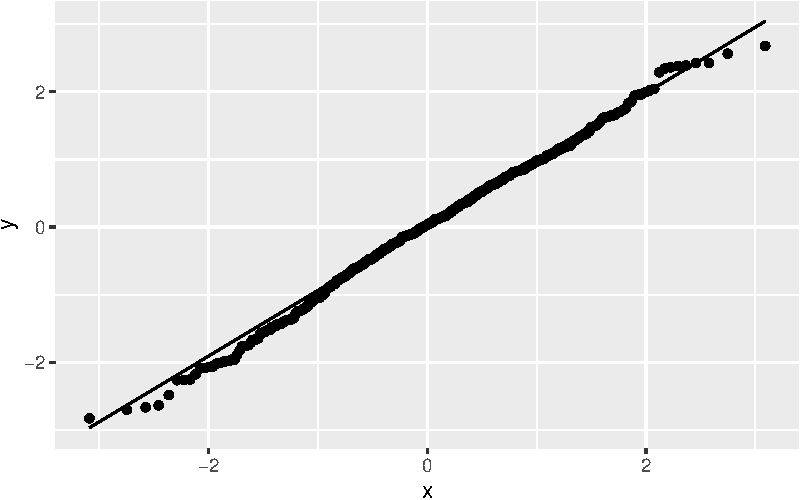
\includegraphics[keepaspectratio]{chapter11_files/figure-pdf/unnamed-chunk-4-1.pdf}}

Q-Qプロットとは2つの確率分布を比較するためのグラフであり,横軸には理論的分布の分位点が,縦軸に実データが並ぶもので,右上がりの直線上にデータが載っていれば分布に従っている,と判断するものである。直線から逸脱している点は理論的分布からの逸脱と考えられる。今回の結果はほとんどが正規分布の直線上にあることから,大きな逸脱がないことが認められる。

データ生成メカニズムによっては,被説明変数が二値的であったり,順序的であったり,カウント変数であったり,と正規分布がそぐわないものもあるだろう。そのようなデータに無理やり回帰分析を当てはめることは適切ではない。いかなる時もデータは可視化して,モデルを当てはめることの適切さをチェックすることを忘れたはならない。

ちなみに出力結果を直接\texttt{plot}関数に入れてもよい。ここから残差と予測値の相関関係や,Q-Qプロット,標準化残差のスケールロケーションプロット,レバレッジと標準化残差\footnote{縦軸の標準化された残差の大きな値は解釈に注意が必要な外れ値である可能性が高い。レバレッジも同様に回帰係数に大きな影響を与える値の指標であり,この図の端に位置する変数は注意が必要,と考える。}
などがプロットされる。

\begin{Shaded}
\begin{Highlighting}[]
\FunctionTok{plot}\NormalTok{(result.lm)}
\end{Highlighting}
\end{Shaded}

\pandocbounded{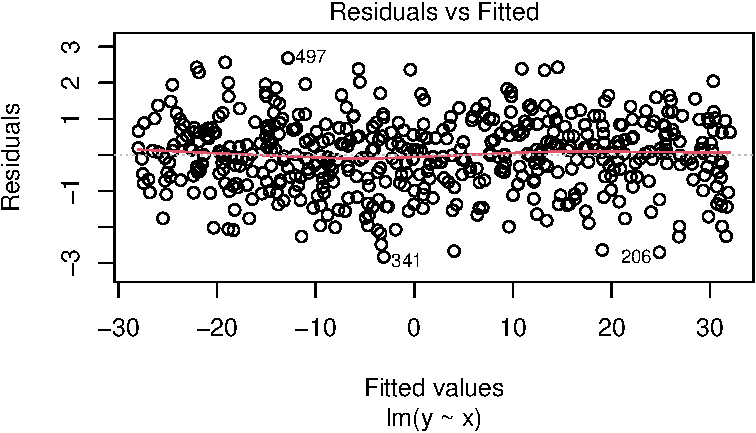
\includegraphics[keepaspectratio]{chapter11_files/figure-pdf/unnamed-chunk-5-1.pdf}}

\pandocbounded{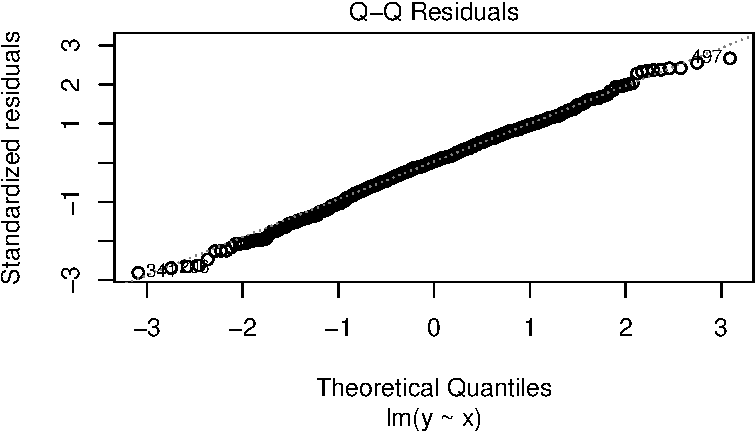
\includegraphics[keepaspectratio]{chapter11_files/figure-pdf/unnamed-chunk-5-2.pdf}}

\pandocbounded{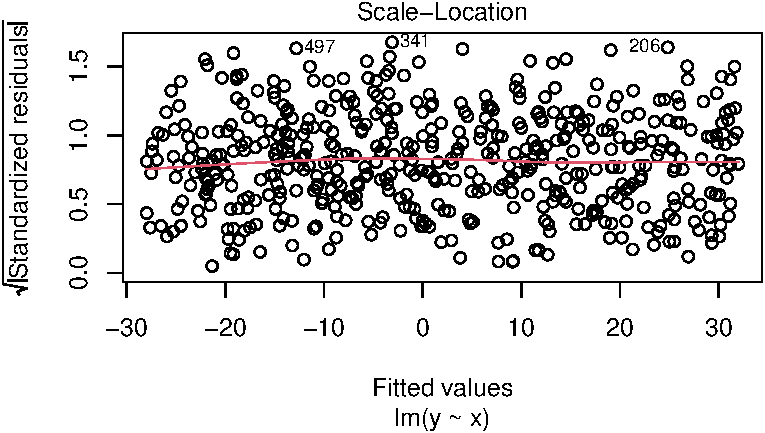
\includegraphics[keepaspectratio]{chapter11_files/figure-pdf/unnamed-chunk-5-3.pdf}}

\pandocbounded{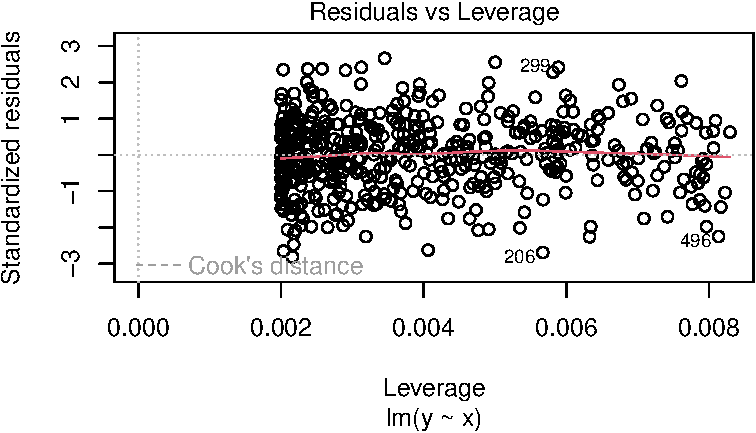
\includegraphics[keepaspectratio]{chapter11_files/figure-pdf/unnamed-chunk-5-4.pdf}}

残差と予測値のプロットからも想像できるが,両者の相関はゼロである。図で確認しておこう。

\begin{Shaded}
\begin{Highlighting}[]
\NormalTok{pacman}\SpecialCharTok{::}\FunctionTok{p\_load}\NormalTok{(GGally) }\CommentTok{\# 必要ならインストールしよう}
\FunctionTok{ggpairs}\NormalTok{(dat)}
\end{Highlighting}
\end{Shaded}

\pandocbounded{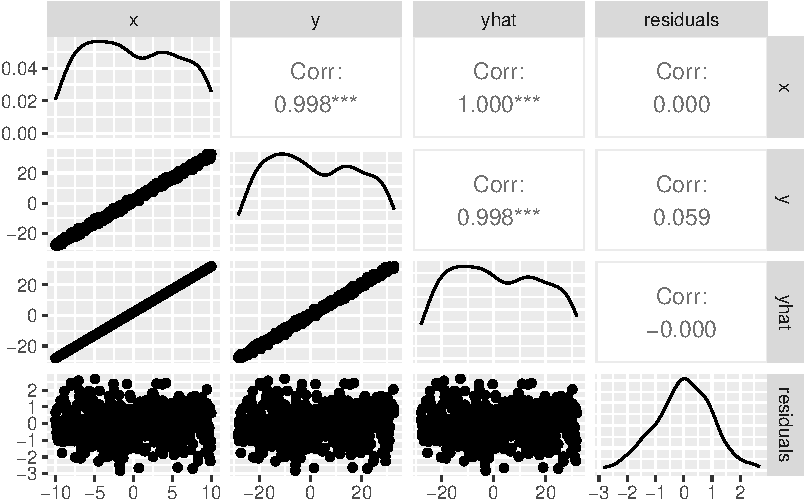
\includegraphics[keepaspectratio]{chapter11_files/figure-pdf/unnamed-chunk-6-1.pdf}}

この関係から明らかなように,残差は説明変数や予測値と相関しない\footnote{もちろん証明できる。詳細は
  \textcite{kosugi2018} を参照すること。}。説明変数と残差に相関関係があるとすると,説明変数でまだ説明できていない分散が残っていることになるし,予測値と残差に相関がないことは予測値が高いか低いかにかかわらず,残差が一様に分布していることを意味する。このことを踏まえて,重回帰分析の特徴を理解していこう。

\section{重回帰分析の特徴}\label{ux91cdux56deux5e30ux5206ux6790ux306eux7279ux5fb4}

重回帰分析においては,回帰係数は偏回帰係数partial regression
coefficientsと呼ばれる。この「偏」の一文字が意味することを考えていこう。

\subsection{回帰係数と偏回帰係数}\label{ux56deux5e30ux4fc2ux6570ux3068ux504fux56deux5e30ux4fc2ux6570}

単回帰分析の回帰係数は,説明変数\(x\)が一単位上昇した時の被説明変数の変化量,と解釈すればよい。これに対して重回帰分析の偏回帰係数を,「説明変数\(x_1\)が一単位上昇した時の被説明変数の変化量」とすることはできない。というのも,説明変数が複数(\(x_2,x_3,\ldots\))あり,他の説明変数の次元についての変化を考慮していない変化量になっているからである。

重回帰分析において,説明変数が完全に無相関で直交しているのであれば,\(x_1\)の変化と\(x_2\)の変化を独立して説明できるが,往々にしてそのようなことはない。偏回帰係数は当該変数以外の変動を\emph{統制した}回帰係数である。

上で単回帰係数において,説明変数と残差が相関しないことを確認した。言い換えれば,説明変数で説明でき分散は全て説明し尽くされており,残差は説明変数で説明できない被説明変数の分散,つまり説明変数の影響を除外した被説明変数の分散と考えることができる(被説明変数の分散=説明変数が説明する分散+残差の分散)。

ここで第二の変数\(x_2\)があったとする。第一の変数\(x_1\)で\(y\)を説明した残差\(e_y\)と,第一の変数で第二の変数を説明した残差\(e_{x2}\)との相関を\textbf{偏相関partial
correlation}という。これは第一の変数\(x_1\)からの影響を両者から取り除いているので,\(x_1\)で統制した相関係数ということができる。偏相関は単純な相関が「見せかけの関係」でないことを検証するための重要な指標である。

偏相関係数を計算してみよう。

\begin{Shaded}
\begin{Highlighting}[]
\NormalTok{pacman}\SpecialCharTok{::}\FunctionTok{p\_load}\NormalTok{(MASS)}
\NormalTok{pacman}\SpecialCharTok{::}\FunctionTok{p\_load}\NormalTok{(psych)}
\NormalTok{Sigma }\OtherTok{\textless{}{-}} \FunctionTok{matrix}\NormalTok{(}\FunctionTok{c}\NormalTok{(}\DecValTok{1}\NormalTok{, }\FloatTok{0.3}\NormalTok{, }\FloatTok{0.5}\NormalTok{, }\FloatTok{0.3}\NormalTok{, }\DecValTok{1}\NormalTok{, }\FloatTok{0.8}\NormalTok{, }\FloatTok{0.5}\NormalTok{, }\FloatTok{0.8}\NormalTok{, }\DecValTok{1}\NormalTok{), }\AttributeTok{ncol =} \DecValTok{3}\NormalTok{)}
\NormalTok{X }\OtherTok{\textless{}{-}} \FunctionTok{mvrnorm}\NormalTok{(}\DecValTok{1000}\NormalTok{, }\FunctionTok{c}\NormalTok{(}\DecValTok{0}\NormalTok{, }\DecValTok{0}\NormalTok{, }\DecValTok{0}\NormalTok{), Sigma, }\AttributeTok{empirical =} \ConstantTok{TRUE}\NormalTok{) }\SpecialCharTok{\%\textgreater{}\%} \FunctionTok{as.data.frame}\NormalTok{()}
\DocumentationTok{\#\# 相関行列}
\FunctionTok{cor}\NormalTok{(X)}
\end{Highlighting}
\end{Shaded}

\begin{verbatim}
    V1  V2  V3
V1 1.0 0.3 0.5
V2 0.3 1.0 0.8
V3 0.5 0.8 1.0
\end{verbatim}

\begin{Shaded}
\begin{Highlighting}[]
\DocumentationTok{\#\# 回帰分析をして残差を求める}
\NormalTok{result.lm1 }\OtherTok{\textless{}{-}} \FunctionTok{lm}\NormalTok{(V2 }\SpecialCharTok{\textasciitilde{}}\NormalTok{ V1, }\AttributeTok{data =}\NormalTok{ X)}
\NormalTok{result.lm2 }\OtherTok{\textless{}{-}} \FunctionTok{lm}\NormalTok{(V3 }\SpecialCharTok{\textasciitilde{}}\NormalTok{ V1, }\AttributeTok{data =}\NormalTok{ X)}
\FunctionTok{cor}\NormalTok{(result.lm1}\SpecialCharTok{$}\NormalTok{residuals, result.lm2}\SpecialCharTok{$}\NormalTok{residuals)}
\end{Highlighting}
\end{Shaded}

\begin{verbatim}
[1] 0.7867958
\end{verbatim}

\begin{Shaded}
\begin{Highlighting}[]
\DocumentationTok{\#\# 偏相関を求めるR関数で確認}
\NormalTok{psych}\SpecialCharTok{::}\FunctionTok{partial.r}\NormalTok{(X)[}\DecValTok{2}\NormalTok{, }\DecValTok{3}\NormalTok{]}
\end{Highlighting}
\end{Shaded}

\begin{verbatim}
[1] 0.7867958
\end{verbatim}

最後は\texttt{psych}パッケージの偏相関行列を求める関数で検証した。確かに残差同士の相関係数が偏相関係数になっていることが確認できたと思う。

そして,ここでは残差同士の相関係数として算出しているが,残差をつかった回帰分析の係数が偏回帰係数になるのである。このデータセットの第一変数を従属変数にした重回帰分析の結果から,これを確認してみよう。

\begin{Shaded}
\begin{Highlighting}[]
\NormalTok{result.mra }\OtherTok{\textless{}{-}} \FunctionTok{lm}\NormalTok{(V1 }\SpecialCharTok{\textasciitilde{}}\NormalTok{ V2 }\SpecialCharTok{+}\NormalTok{ V3, }\AttributeTok{data =}\NormalTok{ X)}
\CommentTok{\# 回帰係数を取り出す}
\NormalTok{result.mra}\SpecialCharTok{$}\NormalTok{coefficients}
\end{Highlighting}
\end{Shaded}

\begin{verbatim}
  (Intercept)            V2            V3 
-5.218050e-17 -2.777778e-01  7.222222e-01 
\end{verbatim}

\begin{Shaded}
\begin{Highlighting}[]
\CommentTok{\# 残差をつかって偏回帰係数を確認する}
\NormalTok{result.lm3 }\OtherTok{\textless{}{-}} \FunctionTok{lm}\NormalTok{(V1 }\SpecialCharTok{\textasciitilde{}}\NormalTok{ V3, }\AttributeTok{data =}\NormalTok{ X)}
\NormalTok{result.lm4 }\OtherTok{\textless{}{-}} \FunctionTok{lm}\NormalTok{(V2 }\SpecialCharTok{\textasciitilde{}}\NormalTok{ V3, }\AttributeTok{data =}\NormalTok{ X)}
\NormalTok{result.lm5 }\OtherTok{\textless{}{-}} \FunctionTok{lm}\NormalTok{(result.lm3}\SpecialCharTok{$}\NormalTok{residuals }\SpecialCharTok{\textasciitilde{}}\NormalTok{ result.lm4}\SpecialCharTok{$}\NormalTok{residuals)}
\CommentTok{\#}
\NormalTok{result.lm5}\SpecialCharTok{$}\NormalTok{coefficients}
\end{Highlighting}
\end{Shaded}

\begin{verbatim}
         (Intercept) result.lm4$residuals 
       -7.925711e-18        -2.777778e-01 
\end{verbatim}

重回帰分析の結果\texttt{result.mra}の\texttt{V2}から\texttt{V1}への回帰係数は-0.2778である。また,\texttt{V3}で\texttt{V1,V2}を統制した残差同士をつかい,回帰係数を求めた結果は-0.2778と,同じ値になっていることが確認できただろう。

\texttt{V3}から\texttt{V1}への偏回帰係数も同様で,\texttt{V2}で両者を統制した残差同士による回帰係数になっている。このように,重回帰分析の回帰係数は,他の説明変数で統制した値になっており,日本語で説明するなら「他の変数の値が同じであると想定した条件つきの,当該変数の影響力」とでもいうべき値になっている。

なぜこのような持って回った説明をするかというと,つい「条件付きの」という話を忘れて報告,解釈してしまうことが多いからで,\textcite{yoshidaMRA}
の論文での指摘は議論を呼んだのは記憶に新しい\footnote{論文が早期公開された後,心理学会が主催するオンラインシンポジウムでは著者とこの論文で取り上げられた論文の著者が登場して,議論が交わされた(日本心理学会YouTubeライブ・話題の論文について著者と語るシリーズ,2021年7月2日20時-21時40分)。平日の夜という設定,早期公開版における議論であったにも関わらず,1700名近い視聴者が参加した。}。
たとえば今回の例でも,回帰係数が-0.2778であったのに対し,\texttt{V1}と\texttt{V2}の単相関が0.3
であったことを思い出そう。符号が反転しているため,解釈は真逆になってしまう。実際の単相関は正の関係であるから,条件付きであることを忘れて「\texttt{V2}は負の影響,\texttt{V3}は正の影響」と表現してしまうと,ミスリーディングなことになるからである。

また,\textcite{Toyoda201706}
は重回帰分析のこうした誤用を避けるために,独立変数を事前に直交化したデザインで行うコンジョイント分析の積極的な利用を提案している。我々が重回帰分析をうまく使いこなせないのであれば,そうした手法も有用であるだろう。

\subsection{多重共線性}\label{ux591aux91cdux5171ux7ddaux6027}

偏回帰係数の解釈が難しい理由の一つは,説明変数同士に相関関係がみられることにある。
特に,説明変数間の相関関係が高くなることは\textbf{多重共線性}Multicollinearityの問題という。この問題は,回帰係数の標準誤差がインフレを起こすことを指す。

例えば先ほどの例で,説明変数\texttt{V2}と\texttt{V3}は相関係数\(0.8\)を持っていた。この時の回帰係数の標準誤差を確認しておこう。

\begin{Shaded}
\begin{Highlighting}[]
\FunctionTok{summary}\NormalTok{(result.mra)}
\end{Highlighting}
\end{Shaded}

\begin{verbatim}

Call:
lm(formula = V1 ~ V2 + V3, data = X)

Residuals:
     Min       1Q   Median       3Q      Max 
-2.59118 -0.54717 -0.03692  0.55044  2.90735 

Coefficients:
              Estimate Std. Error t value Pr(>|t|)    
(Intercept) -5.218e-17  2.690e-02   0.000        1    
V2          -2.778e-01  4.486e-02  -6.192 8.65e-10 ***
V3           7.222e-01  4.486e-02  16.100  < 2e-16 ***
---
Signif. codes:  0 '***' 0.001 '**' 0.01 '*' 0.05 '.' 0.1 ' ' 1

Residual standard error: 0.8507 on 997 degrees of freedom
Multiple R-squared:  0.2778,    Adjusted R-squared:  0.2763 
F-statistic: 191.7 on 2 and 997 DF,  p-value: < 2.2e-16
\end{verbatim}

標準誤差は0.0449であり,それほど大きくない標準誤差で問題がないようである。しかし両者の相関係数がより高くなり,一方が他方に線形的に従属してしまうと係数の推定値が不安定になるため,注意が必要である。

このインフレを確認するための指標がVariance Infration Factor:
VIFである。Rでは\texttt{car}パッケージにある\texttt{vif}関数に重回帰モデルを入れることでこの指標が算出される。一般にVIFが3,あるいは10を超えると多重共線性が生じており,解釈に注意が必要と言われている\footnote{2変数重回帰分析モデルで,VIFが3であれば説明変数間の相関は\(r=0.81\)程度である。VIFが10であれば\(r=0.97\)にもなる。詳しくは
  \textcite{kosugi2023} を参照。}。

\begin{Shaded}
\begin{Highlighting}[]
\NormalTok{pacman}\SpecialCharTok{::}\FunctionTok{p\_load}\NormalTok{(car) }\CommentTok{\# なければ入れておこう}
\FunctionTok{vif}\NormalTok{(result.mra)}
\end{Highlighting}
\end{Shaded}

\begin{verbatim}
      V2       V3 
2.777778 2.777778 
\end{verbatim}

幸い,今回の値はこれらの基準を下回っていたので許容範囲内である。

\subsection{変数の投入順序}\label{ux5909ux6570ux306eux6295ux5165ux9806ux5e8f}

重回帰分析の場合は複数の説明変数があるが,これを投入するときに全ての変数を同時に投入するか,順番をつけて投入するかといった手法の違いがある。前者を強制投入法と呼ぶこともある。
順番をつけて投入する方法は,逐次投入と呼ばれる。この場合は,適合度指標などを参考に変数を追加あるいは削除して,適合度が統計的に有意に向上するかどうかを考えながら進めていく。

重回帰係数の予測値\(\hat{y}\)と,被説明変数\(y\)の相関係数\(R_{y\hat{y}}\)は\textbf{重相関係数}と呼ばれ,予測がうまくいっているかどうかを表す適合度の一つである。相関係数なので\(-1\)から\(+1\)までの値を取りうるが,\(-1\)は逆に完全に合致していることになるので,この相関係数の符号は大して情報を持たない。そこでこれを二乗した\(R_{y\hat{y}}^2\)を考える。これは\textbf{決定係数}とも呼ばれ,説明変数の分散のうち予測値の分散が占める割合を表している。\footnote{もちろん証明できる。\textcite{kosugi2018}
  を参照。}

説明変数の逐次投入は,説明変数を持たないヌルモデルから一つずつ追加していくForward
Selection,全ての変数を投入してから一つずつ減らしていくBackward
Selectionがある。Forwardのほうは追加することによって\(R^2\)が有意に増加するか,Backwardのほうは削除しても有意に\(R^2\)が減らないか,を確認しながら進めることになる。この方法は手元のデータに最も適した説明変数のペアを選出できる方法ではあるが,検定を繰り返していることの問題と,手元のデータ以外に一般化する時の根拠の乏しさから,用いられないこともある。

逐次投入法には別の観点からの手法もある。それが階層的回帰分析である。この手法は,重回帰分析における交互作用項の投入を検討する文脈で発展した。重回帰分析では,説明変数同士の相関がない,もしくは小さい方が望ましい。しかし,交互作用とは分散分析における組み合わせの効果を表すものであり,実験デザインによっては交互作用効果が重要な変動であることも少なくない。回帰分析と分散分析は,一般線形モデルという形で統一的に理解されるが,回帰分析でも連続的に変化する組み合わせの効果を考えることができる。交互作用があるということは説明変数間に相関があることを意味するため,回帰分析の大前提に抵触する可能性があり,その投入には慎重を期する必要がある。

こうした文脈から,まずは要因の効果を投入し,次に交互作用項を投入してモデル適合度の有意な改善がみられるかどうかを検証する手順が推奨されている。この逐次投入法を特に階層的回帰分析と呼ぶ。ここでの「階層」とは,手順が重要度順に進められていることを意味し,データの特徴に関するものではないことに注意が必要である\footnote{これに対して,データの階層性(ex.学級\(\subset\)市区町村\(\subset\)都道府県)を考慮する線形モデルのことを,階層線形モデルHierarchical
  Linear Model:HLM という。}。

\section{係数の標準誤差と検定}\label{ux4fc2ux6570ux306eux6a19ux6e96ux8aa4ux5deeux3068ux691cux5b9a}

\subsection{係数の検定}\label{ux4fc2ux6570ux306eux691cux5b9a}

サンプルが母集団から得られた確率変数であるのだから,(偏)回帰係数もまた確率変数である。すなわち,サンプルが変わるごとに変化し,その揺らぎがある確率分布に従うと考えられる。これを確認するためには,データ生成過程をモデリングし,反復することで近似させて理解するのがいいだろう。

\begin{Shaded}
\begin{Highlighting}[]
\FunctionTok{set.seed}\NormalTok{(}\DecValTok{123}\NormalTok{)}
\NormalTok{n }\OtherTok{\textless{}{-}} \DecValTok{500}
\NormalTok{beta0 }\OtherTok{\textless{}{-}} \DecValTok{2}
\NormalTok{beta1 }\OtherTok{\textless{}{-}} \DecValTok{3}
\NormalTok{sigma }\OtherTok{\textless{}{-}} \DecValTok{1}
\CommentTok{\# データ生成関数}
\NormalTok{dataMake }\OtherTok{\textless{}{-}} \ControlFlowTok{function}\NormalTok{(n, beta0, beta1, sigma) \{}
\NormalTok{  x }\OtherTok{\textless{}{-}} \FunctionTok{runif}\NormalTok{(n, }\SpecialCharTok{{-}}\DecValTok{10}\NormalTok{, }\DecValTok{10}\NormalTok{)}
\NormalTok{  e }\OtherTok{\textless{}{-}} \FunctionTok{rnorm}\NormalTok{(n, }\DecValTok{0}\NormalTok{, sigma)}
\NormalTok{  y }\OtherTok{\textless{}{-}}\NormalTok{ beta0 }\SpecialCharTok{+}\NormalTok{ beta1 }\SpecialCharTok{*}\NormalTok{ x }\SpecialCharTok{+}\NormalTok{ e}
\NormalTok{  dat }\OtherTok{\textless{}{-}} \FunctionTok{data.frame}\NormalTok{(x, y)}
  \FunctionTok{return}\NormalTok{(dat)}
\NormalTok{\}}

\CommentTok{\# 結果オブジェクトの準備}
\NormalTok{iter }\OtherTok{\textless{}{-}} \DecValTok{2000}
\NormalTok{beta0.est }\OtherTok{\textless{}{-}} \FunctionTok{rep}\NormalTok{(}\ConstantTok{NA}\NormalTok{, iter)}
\NormalTok{beta1.est }\OtherTok{\textless{}{-}} \FunctionTok{rep}\NormalTok{(}\ConstantTok{NA}\NormalTok{, iter)}
\CommentTok{\# simulation}
\ControlFlowTok{for}\NormalTok{ (i }\ControlFlowTok{in} \DecValTok{1}\SpecialCharTok{:}\NormalTok{iter) \{}
\NormalTok{  sample }\OtherTok{\textless{}{-}} \FunctionTok{dataMake}\NormalTok{(n, beta0, beta1, sigma)}
\NormalTok{  result.lm }\OtherTok{\textless{}{-}} \FunctionTok{lm}\NormalTok{(y }\SpecialCharTok{\textasciitilde{}}\NormalTok{ x, }\AttributeTok{data =}\NormalTok{ sample)}
\NormalTok{  beta0.est[i] }\OtherTok{\textless{}{-}}\NormalTok{ result.lm}\SpecialCharTok{$}\NormalTok{coefficients[}\DecValTok{1}\NormalTok{]}
\NormalTok{  beta1.est[i] }\OtherTok{\textless{}{-}}\NormalTok{ result.lm}\SpecialCharTok{$}\NormalTok{coefficients[}\DecValTok{2}\NormalTok{]}
\NormalTok{\}}

\FunctionTok{data.frame}\NormalTok{(}\AttributeTok{x =}\NormalTok{ beta0.est) }\SpecialCharTok{\%\textgreater{}\%} \FunctionTok{ggplot}\NormalTok{(}\FunctionTok{aes}\NormalTok{(}\AttributeTok{x =}\NormalTok{ x)) }\SpecialCharTok{+}
  \FunctionTok{geom\_histogram}\NormalTok{()}
\end{Highlighting}
\end{Shaded}

\begin{verbatim}
`stat_bin()` using `bins = 30`. Pick better value with `binwidth`.
\end{verbatim}

\pandocbounded{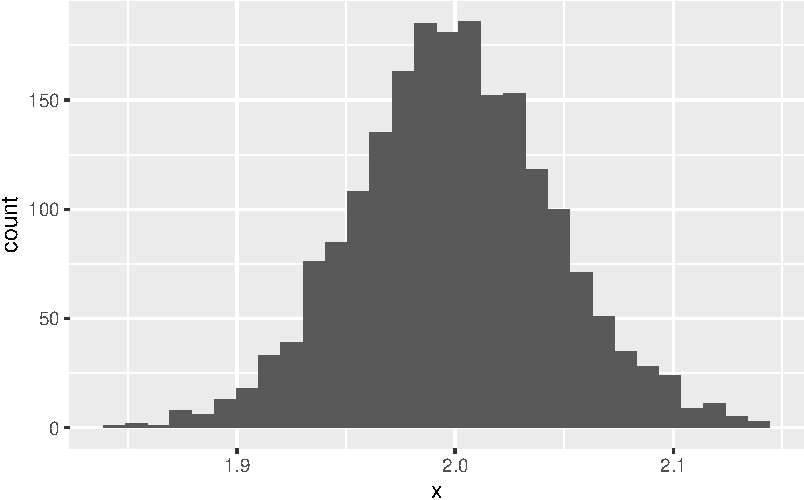
\includegraphics[keepaspectratio]{chapter11_files/figure-pdf/unnamed-chunk-11-1.pdf}}

\begin{Shaded}
\begin{Highlighting}[]
\FunctionTok{data.frame}\NormalTok{(}\AttributeTok{x =}\NormalTok{ beta1.est) }\SpecialCharTok{\%\textgreater{}\%} \FunctionTok{ggplot}\NormalTok{(}\FunctionTok{aes}\NormalTok{(}\AttributeTok{x =}\NormalTok{ x)) }\SpecialCharTok{+}
  \FunctionTok{geom\_histogram}\NormalTok{()}
\end{Highlighting}
\end{Shaded}

\begin{verbatim}
`stat_bin()` using `bins = 30`. Pick better value with `binwidth`.
\end{verbatim}

\pandocbounded{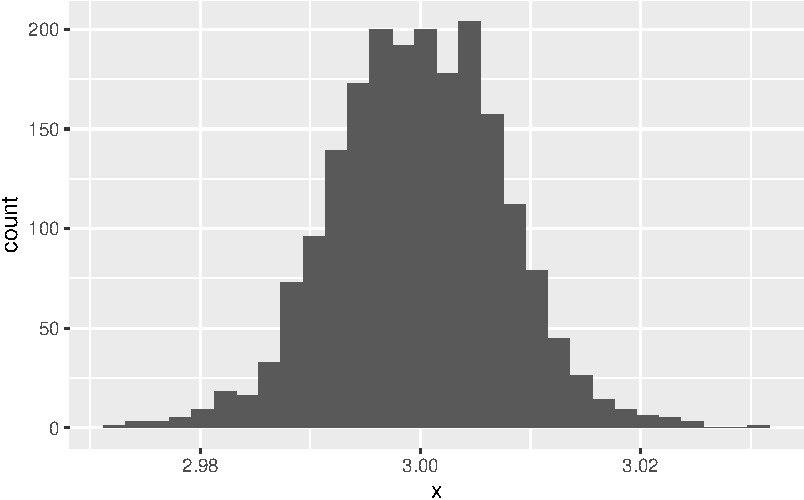
\includegraphics[keepaspectratio]{chapter11_files/figure-pdf/unnamed-chunk-11-2.pdf}}

図から明らかなように,回帰係数も確率的に分布する。ただしその平均は理論値に近似している。

\begin{Shaded}
\begin{Highlighting}[]
\FunctionTok{mean}\NormalTok{(beta0.est)}
\end{Highlighting}
\end{Shaded}

\begin{verbatim}
[1] 1.999257
\end{verbatim}

\begin{Shaded}
\begin{Highlighting}[]
\FunctionTok{mean}\NormalTok{(beta1.est)}
\end{Highlighting}
\end{Shaded}

\begin{verbatim}
[1] 2.999798
\end{verbatim}

この分布の幅が回帰係数の標準誤差である。

\begin{Shaded}
\begin{Highlighting}[]
\FunctionTok{sd}\NormalTok{(beta0.est)}
\end{Highlighting}
\end{Shaded}

\begin{verbatim}
[1] 0.04580387
\end{verbatim}

\begin{Shaded}
\begin{Highlighting}[]
\FunctionTok{sd}\NormalTok{(beta1.est)}
\end{Highlighting}
\end{Shaded}

\begin{verbatim}
[1] 0.007659277
\end{verbatim}

回帰係数はt分布に従い,その自由度はサンプルサイズからモデルで用いる係数の数を引いたものになる。先ほどのヒストグラムを基準化し,理論分布を重ねて描画してみることで確認しておこう。

\begin{Shaded}
\begin{Highlighting}[]
\FunctionTok{data.frame}\NormalTok{(}\AttributeTok{x =}\NormalTok{ beta1.est) }\SpecialCharTok{\%\textgreater{}\%}
  \FunctionTok{scale}\NormalTok{() }\SpecialCharTok{\%\textgreater{}\%}
  \FunctionTok{ggplot}\NormalTok{(}\FunctionTok{aes}\NormalTok{(}\AttributeTok{x =}\NormalTok{ x)) }\SpecialCharTok{+}
  \FunctionTok{geom\_histogram}\NormalTok{(}\FunctionTok{aes}\NormalTok{(}\AttributeTok{y =} \FunctionTok{after\_stat}\NormalTok{(density)), }\AttributeTok{bins =} \DecValTok{100}\NormalTok{) }\SpecialCharTok{+}
  \FunctionTok{stat\_function}\NormalTok{(}\AttributeTok{fun =} \ControlFlowTok{function}\NormalTok{(x) }\FunctionTok{dt}\NormalTok{(x, }\AttributeTok{df =}\NormalTok{ n }\SpecialCharTok{{-}} \DecValTok{2}\NormalTok{), }\AttributeTok{color =} \StringTok{"red"}\NormalTok{, }\AttributeTok{linewidth =} \DecValTok{2}\NormalTok{)}
\end{Highlighting}
\end{Shaded}

\pandocbounded{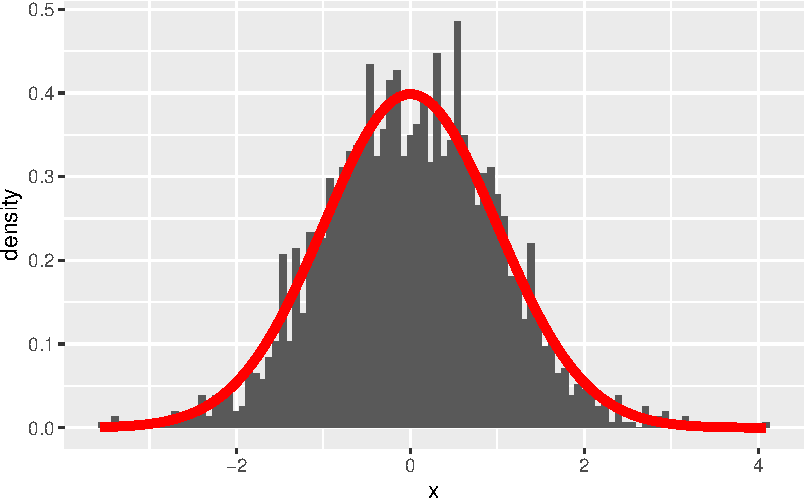
\includegraphics[keepaspectratio]{chapter11_files/figure-pdf/unnamed-chunk-14-1.pdf}}

このt分布を用いて,係数が0の母集団から得られたサンプルなのかどうかの検定が行われる。

\subsection{モデル適合度の検定}\label{ux30e2ux30c7ux30ebux9069ux5408ux5ea6ux306eux691cux5b9a}

一方で,出力の最後にはF統計量による検定も行われていたことを確認しておこう。次に示すのは重回帰分析の例である。

\begin{Shaded}
\begin{Highlighting}[]
\FunctionTok{set.seed}\NormalTok{(}\DecValTok{123}\NormalTok{)}
\NormalTok{n }\OtherTok{\textless{}{-}} \DecValTok{500}
\NormalTok{beta0 }\OtherTok{\textless{}{-}} \DecValTok{2}
\NormalTok{beta1 }\OtherTok{\textless{}{-}} \DecValTok{0}
\NormalTok{beta2 }\OtherTok{\textless{}{-}} \DecValTok{0}
\NormalTok{sigma }\OtherTok{\textless{}{-}} \DecValTok{1}
\NormalTok{x1 }\OtherTok{\textless{}{-}} \FunctionTok{runif}\NormalTok{(n, }\SpecialCharTok{{-}}\DecValTok{10}\NormalTok{, }\DecValTok{10}\NormalTok{)}
\NormalTok{x2 }\OtherTok{\textless{}{-}} \FunctionTok{runif}\NormalTok{(n, }\SpecialCharTok{{-}}\DecValTok{10}\NormalTok{, }\DecValTok{10}\NormalTok{)}
\NormalTok{e }\OtherTok{\textless{}{-}} \FunctionTok{rnorm}\NormalTok{(n, }\DecValTok{0}\NormalTok{, sigma)}
\NormalTok{y }\OtherTok{\textless{}{-}}\NormalTok{ beta0 }\SpecialCharTok{+}\NormalTok{ beta1 }\SpecialCharTok{*}\NormalTok{ x1 }\SpecialCharTok{+}\NormalTok{ beta2 }\SpecialCharTok{*}\NormalTok{ x2 }\SpecialCharTok{+}\NormalTok{ e}
\NormalTok{sample }\OtherTok{\textless{}{-}} \FunctionTok{data.frame}\NormalTok{(y, x1, x2)}
\NormalTok{result.lm }\OtherTok{\textless{}{-}} \FunctionTok{lm}\NormalTok{(y }\SpecialCharTok{\textasciitilde{}}\NormalTok{ x1 }\SpecialCharTok{+}\NormalTok{ x2, }\AttributeTok{data =}\NormalTok{ sample)}
\FunctionTok{summary}\NormalTok{(result.lm)}
\end{Highlighting}
\end{Shaded}

\begin{verbatim}

Call:
lm(formula = y ~ x1 + x2, data = sample)

Residuals:
     Min       1Q   Median       3Q      Max 
-2.85235 -0.68275 -0.01436  0.67809  2.70488 

Coefficients:
             Estimate Std. Error t value Pr(>|t|)    
(Intercept)  1.996999   0.045263  44.120   <2e-16 ***
x1          -0.006453   0.007970  -0.810    0.418    
x2          -0.003928   0.007795  -0.504    0.615    
---
Signif. codes:  0 '***' 0.001 '**' 0.01 '*' 0.05 '.' 0.1 ' ' 1

Residual standard error: 1.012 on 497 degrees of freedom
Multiple R-squared:  0.001893,  Adjusted R-squared:  -0.002124 
F-statistic: 0.4713 on 2 and 497 DF,  p-value: 0.6245
\end{verbatim}

上の例では,統計量\(F\)が,自由度\(F(\) 2,497
\()\)のもとで,0.4713であり,統計的に有意ではないと判断される(p=0.6245,n.s.)。

これは重相関係数に対する検定であり,母集団においてモデル全体としての説明力が0である,という帰無仮説を検証しているものである。この有意性検定には,説明変数の数\(p\),サンプルサイズ\(n\),重相関係数\(R^2\)を用いて,以下の式で用いられる検定統計量Fを利用する\autocite{Haebara2014}。

\[ F= \frac{R^2}{1-R^2}\cdot\frac{n-p-1}{p} \]

ここで右辺第一項目はCohenの効果量(\(f^2=\frac{R^2}{1-R^2}\))
といわれ,サンプルサイズ設計においてはこの指標が利用される。

\section{サンプルサイズ設計}\label{ux30b5ux30f3ux30d7ux30ebux30b5ux30a4ux30baux8a2dux8a08-1}

重回帰分析のサンプルサイズ設計は,変数の効果の大きさ(回帰係数)が事前にわかっているのであれば,nを徐々に増やしていくシミュレーションによって行える。しかしそのようなケースは稀であり,実際には\(R^2\)の検定を用いて,ある効果量と検出力の下で,正しく検出できるサイズを算出することになる。

サンプルサイズの算出には,非心F分布を用いる。この時の非心度は,効果量\(f^2\)に\(n\)をかけたものになる。これを使ってサンプルサイズ設計をする例は以下のとおりである。

\begin{Shaded}
\begin{Highlighting}[]
\NormalTok{f2 }\OtherTok{\textless{}{-}} \FloatTok{0.15} \CommentTok{\# 効果量}
\NormalTok{alpha }\OtherTok{\textless{}{-}} \FloatTok{0.05} \CommentTok{\# タイプ1エラー率}
\NormalTok{beta }\OtherTok{\textless{}{-}} \FloatTok{0.2} \CommentTok{\# タイプ2エラー率}
\NormalTok{p }\OtherTok{\textless{}{-}} \DecValTok{5} \CommentTok{\# 説明変数の数}

\ControlFlowTok{for}\NormalTok{ (n }\ControlFlowTok{in} \DecValTok{10}\SpecialCharTok{:}\DecValTok{500}\NormalTok{) \{}
\NormalTok{  lambda }\OtherTok{\textless{}{-}}\NormalTok{ f2 }\SpecialCharTok{*}\NormalTok{ n}
\NormalTok{  df1 }\OtherTok{\textless{}{-}}\NormalTok{ p}
\NormalTok{  df2 }\OtherTok{\textless{}{-}}\NormalTok{ n }\SpecialCharTok{{-}}\NormalTok{ p }\SpecialCharTok{{-}} \DecValTok{1}
\NormalTok{  cv }\OtherTok{\textless{}{-}} \FunctionTok{qf}\NormalTok{(}\AttributeTok{p =} \DecValTok{1} \SpecialCharTok{{-}}\NormalTok{ alpha, df1, df2)}
\NormalTok{  t2error }\OtherTok{\textless{}{-}} \FunctionTok{pf}\NormalTok{(}\AttributeTok{q =}\NormalTok{ cv, df1, df2, }\AttributeTok{ncp =}\NormalTok{ lambda)}
  \ControlFlowTok{if}\NormalTok{ (t2error }\SpecialCharTok{\textless{}}\NormalTok{ beta) \{}
    \ControlFlowTok{break}
\NormalTok{  \}}
\NormalTok{\}}

\FunctionTok{print}\NormalTok{(n)}
\end{Highlighting}
\end{Shaded}

\begin{verbatim}
[1] 92
\end{verbatim}

この設定では,n =
92以上であればモデルとして影響力がないとは言えない,ということがわかる。

\section{まとめ}\label{ux307eux3068ux3081}

重回帰分析は,人文社会科学で多用される技術ではあるが,技術が先行して理解が伴わないまま利用されているケースも少なくない。繰り返しになる点もあるが,以下に注意点をまとめておく。

\begin{itemize}
\tightlist
\item
  \textbf{偏回帰係数の意味};重回帰分析における偏回帰係数は,ほかの変数を統制した上での値であり,あたかも各係数が独立直交しているかのように解釈するのは適切ではない。
\item
  \textbf{誤差の正規性};誤差は正規分布に従っているという仮定があり,二値データや整数しかとらないカウントデータなどに盲目的にモデルを適用してはならない。誤差の正規性が満たされているかどうかは,分析後にQ-Qプロットを用いて確認する。
\item
  \textbf{誤差の均質性};誤差はモデル全体にわたって同じ正規分布に従っているというのもモデルの仮定である。すなわち,独立変数に応じて誤差分散が変わるといった均質でないデータの場合は,正しく推定されない。誤差の均質性については,分析後のQ-Qプロットを用いて確認する。
\item
  \textbf{誤差間の独立性};誤差はモデル全体にわたって同じ正規分布から独立に生成されている(i.i.d)というのがモデルの仮定である。時系列データのように,誤差間に対応(自己回帰)がみられるデータの場合は回帰分析は適切な手法とならない。状態空間モデルなど,誤差間関係を適切にモデリングしたものを当てはめる必要がある。
\item
  \textbf{モデルの適切な定式化};モデルには被説明変数に影響を与えるすべての変数が正しく含まれている必要がある。例えば,影響を与えることがわかっている変数\(X_o\)を意図的に除外して分析をしたとする。そのモデルに含まれる変数\(X_a\)が被説明変数\(y\)に影響を与えていたとしても,\(X_a\)と\(X_o\)に相関があれば,\(X_o\)の影響力が\(X_a\)を通じて\(y\)に伝播するkから,\(X_a\)の影響力が課題に評価されることになる。自らの仮説のために,意図的に変数を選択するのはQRPsに該当する。
\item
  \textbf{説明変数間の相関関係};説明変数のうちにあまりにも相関関係が高い変数ペアがあれば,多重共線性の疑いが生じる。多重共線性は推定値の不安定さとなって現れる。このような場合は,説明変数を主成分分析で合成変数にまとめるといった対応が考えられる。また,高い相関ではないが交互作用効果が見たいといった場合は,逐次投入など慎重に個々の影響を考えながら投入するようにする(階層的重回帰分析)。なお交互作用項は,各変数の平均からの偏差をかけ合わせたものにすることが一般的である。
\end{itemize}

\section{課題}\label{ux8ab2ux984c-9}

\begin{enumerate}
\def\labelenumi{\arabic{enumi}.}
\tightlist
\item
  以下のデータセットは被説明変数\(y\),説明変数\(x1,x2\)からなる重回帰分析のサンプルデータです。画面には一部しか表示しておらず,全体(\(n=100\))はこちら\url{ex_regression1.csv}からダウンロード可能です。このデータセットを用いて重回帰分析を行い,結果を出力してください。
\end{enumerate}

\begin{verbatim}
           y        x1         x2
1  1.8685595 -4.248450  1.9997792
2 -0.5728781  5.766103 -3.3435292
3  1.0321850 -1.820462 -0.2277393
4 10.0468488  7.660348  9.0894765
5 -1.1968078  8.809346 -0.3419521
6  9.6719213 -9.088870  7.8070044
\end{verbatim}

\begin{enumerate}
\def\labelenumi{\arabic{enumi}.}
\setcounter{enumi}{1}
\tightlist
\item
  以下のデータセットは被説明変数\(y\),説明変数\(x1,x2\)からなる重回帰分析のサンプルデータです。画面には一部しか表示しておらず,全体(\(n=300\))はこちら\url{ex_regression2.csv}からダウンロード可能です。このデータセットを用いて重回帰分析を行ってください。結果のプロットから,上に挙げた重回帰分析の仮定に反しているところを指摘してください。
\end{enumerate}

\begin{verbatim}
          y         x1           x2
1  3.586304 -0.4248450  0.132767341
2  8.599252  0.5766103  0.922713561
3  2.397115 -0.1820462  0.053684622
4  3.505236  0.7660348  0.007801881
5  6.517720  0.8809346  0.633076091
6 -1.394231 -0.9088870 -0.895346802
\end{verbatim}

\begin{enumerate}
\def\labelenumi{\arabic{enumi}.}
\setcounter{enumi}{2}
\tightlist
\item
  \(R^2=0.3\)を目標として,説明変数の数\(p=10\)の重回帰分析を行う際に,必要なサンプルサイズはいくつになるか,計算してみましょう。ここで,\(\alpha = 0.05,\beta=0.2\)とします。
\end{enumerate}

\bookmarksetup{startatroot}

\chapter{ベイズ統計の活用}\label{ux30d9ux30a4ux30baux7d71ux8a08ux306eux6d3bux7528}

ここまで心理統計の基本的な話題をRで実践しながら見てきたが,ここでベイズ統計の話題を導入しよう。
わざわざこのように断る理由は,ベイズ統計学が推測統計学の枠組みの一種であるにもかかわらず,その歴史や解釈によって様々な誤解が生じているからである。一説にはベイズ統計学には100を超える派閥・解釈のスタイルがあるとも言われており,迂闊に議論をすることが憚られるような言説が交わされることも少なくない。

筆者はファッションベイジアンを自認しており,主義主張を戦わせることはあまり好ましいことではないと考えている。そのような調子の良い立場の人間が語ることである,という事前情報を十分理解した上で,以下の解説を読んでほしい。

\section{ベイズ統計の位置付け}\label{ux30d9ux30a4ux30baux7d71ux8a08ux306eux4f4dux7f6eux4ed8ux3051}

ベイズ統計学の生まれは古く,ベイズの定理にまで遡れば実に300年近く前になる。ベイズの定理を見出したとされるトーマス・ベイズは,18世紀の牧師であり,1763年に死んでいる。その古い人物の名を冠した定理が,現在は「ベイズ統計学」と学問全体を覆うほどになっているのは,それがこれまで紹介してきた統計モデルと考え方や解釈の仕方を大幅に変えているからである。

また,ベイズ統計学はその長い歴史に対して,応用的な価値が見出されたのが比較的最近である。筆者の感覚で言えば,2010年以降になって,ベイズ統計学の応用が急速に広まったように思う。古くから知られていた理論が長らくその名をひそめていたのは,ベイズ統計学を応用できるシーンが限定的であったこと,その研究が軍事的な機密を含むことで公開されることが少なかったこと,そして冗談のように聞こえるかもしれないが,アメリカ統計学会の重鎮がベイズ統計学を嫌っていたこと,がその理由と考えられる。このあたりの事情については\autocite{mcgrayne2011theory}を参考にしてほしい。

そして近年になって改めてベイズ統計学が注目されるようになったのには,2つの理由がある。第一は社会心理学における再現性の危機に対する対応として,従来の統計学ではない新しいアプローチとして期待されたこと。第二は計算機科学の発展により,非常にパワフルな推定方法が開発され,統計モデルを非常に柔軟に扱うことができるようになったこと,である。

再現性の危機に対する対応としてのベイズ統計学は,従来の統計学を「頻度主義的」なものとして,ベイズ統計学を「ベイズ主義的」なものとして区別することで,その違いを強調するきらいがある。しかし,頻度主義的な方法に問題があるからという単純な理由でベイズ主義的な方法に乗り換えると,そもそもの問題であった統計法の悪用や誤用の種類が変わるだけに過ぎない。

筆者は教育的観点から,ベイズ主義的な統計学の方が初学者には優しく,より理解しやすいのではないかと考えている。しかし,心理学のこの100年の歴史の中で積み重ねられてきた「頻度主義的」な研究のお作法は,誤用悪用を招く恐れもあるとは言え,非常にリッチな教育コンテンツ,分析ツールを提供してきた。またこれまでの心理学的文献が「頻度主義的」なものであったことを考えると,これらを捨て去って心機一転,一気にベイズに乗り換えようというのは現実的ではない。ベイズ統計学の弱点としては,教育コンテンツ,分析ツール,そしてベイズ統計学の教育者がそもそも少ないこと,が挙げられる。もちろんこれらの問題点が,近い将来のうちに解決されることを望むものである。

第二の理由はベイズ統計学のポジティブな未来を予感させる。統計モデルが複雑になるにつれ,最尤推定法は実質的な限界を迎えるときでも,ベイズ推定の新しいアプローチは対応できる。これは,ベイズ統計学のパワーを具現化する計算機手法,すなわちMCMC法の発展によるところが大きい。統計モデルを非常に柔軟に,自らの研究データにカスタマイズした分析モデルを構築でき,その他のモデルともベイズファクターという一元的な指標で評価できることは,ベイズ統計学の大きな魅力である。しかし反面,細かく統計モデルをカスタマイズできるということは,研究者にプログラマとしての技量を要求することになる。心理学者はあくまでも統計をツールとして使いたいユーザなのだから,ソフトウェア的なエンジニアリングにあまりエフォートをかけていられないということもあるだろう。しかし,平均値の差の検定や要因計画にとらわれない,自由なモデリングができる魅力はおおきく,心理学の中でも統計モデリングによるアプローチをとる人も年々増加傾向にある。

\section{MCMC法}\label{mcmcux6cd5}

ベイズ統計を広く応用できるようにした,革新的な技術であるMCMC法についてみていこう。その前に,ベイズの定理を使った考え方について基本的な説明をしておく。

\subsection{ベイズの定理}\label{ux30d9ux30a4ux30baux306eux5b9aux7406}

ベイズの定理は,条件付き確率の定理である。ある事象\(A\)が起きたときに,事象\(B\)が起きる確率を\(P(B|A)\)と表すと,ベイズの定理は以下のように表される。

\[
P(B|A) = \frac{P(A|B)P(B)}{P(A)}
\]

ここで,\(P(A)\)は事象\(A\)が起きる確率,\(P(B)\)は事象\(B\)が起きる確率,\(P(A|B)\)は事象\(B\)が起きたときに事象\(A\)が起きる確率,\(P(B|A)\)は事象\(A\)が起きたときに事象\(B\)が起きる確率を表す。ここでの重要な点は,この式の右辺と左辺とで,条件付き確率の位置が変わっていることである。

この式は,事象\(A\)が起きたときに事象\(B\)が起きる確率\(P(B|A)\)を,事象\(B\)が起きたときに事象\(A\)が起きる確率\(P(A|B)\)と,事象\(B\)が起きる確率\(P(B)\)と,事象\(A\)が起きる確率\(P(A)\)を用いて表している。ここで\(A\)をデータ,\(B\)をモデルのパラメータと考えると,ベイズの定理は以下のように表される。

\[
P(\theta|D) = \frac{P(D|\theta)P(\theta)}{P(D)}
\]

この式の左辺にあるのは,データ\(D\)が与えられた時のパラメータ\(\theta\)が得られる確率であり,データに基づいてパラメータを推論するという推測統計学の基本的な考え方である。これを構成する右辺は,\(P(D|\theta)\)はパラメータ\(\theta\)が与えられた時のデータ\(D\)が得られる確率,\(P(\theta)\)はパラメータ\(\theta\)が得られる確率と言える。パラメータ\(\theta\)がある値になったときに,データ\(D\)が得られる確率\(P(D|\theta)\)は尤度と考えることができる。それにかけられる\(P(\theta)\)は,パラメータ\(\theta\)の事前確率と呼ばれるが,これがあることによってベイズ統計学の特徴がより鮮明になる。

データを取る前にパラメータがどのようにあるのか,この不確実さをベイズ統計学では事前確率,あるいは一般に事前分布として表現する。それと尤度を掛け合わせたものが(周辺尤度\(P(D)\)で除されるとは言え)統計的な推測の結果である事後確率,事後分布\(P(\theta|D)\)となっている。

古典的には,データを取る前にパラメータのあり方を想定するのは,科学的な態度として不適切であるとして,ベイズ統計学は批判されてきた。この点を認めたとして,改めて式を見てみると,確率分布とデータの関係を表す尤度に,事前分布と周辺尤度の比をかけた結果,事後分布が得られていることになる。尤度を計算してその最も高い値を持つパラメータを推定値としよう,というのが最尤推定法だったわけだが,ベイズ推定はその拡張で,尤度から得られる結果を分布として考えるために事前分布と周辺尤度の比を掛け合わせた,とも言える。尤度関数は確率関数ではないので,そのピークになるところを推定値として用いることしかできなかったが,ベイズの定理を経由すると結果的に得られるのが確率分布になるのだから,パラメータがどのあたりにありそうか,その分布として定量的に評価することも可能である。

\subsection{ベイズの定理の実践史}\label{ux30d9ux30a4ux30baux306eux5b9aux7406ux306eux5b9fux8df5ux53f2}

ベイズ統計学では,未知なるものを確率で表現する。心理統計では平均値パラメータや,複数の平均値パラメータ間の差をすることが目的であり,データを取っただけでは母数が未知なものだったわけだから,これを確率分布として表現することがベイズ統計の最初のステップである。

ベイズ統計は,「未知なるパラメータを確率で表現する(事前分布)」「データによって事前分布を事後分布にアップデートする」というたった2つのステップを繰り返すだけである。事前分布も,データの得られた状況に応じて適切に選択することができる。例えば男性と女性の平均身長の差を知りたい,という状況を考えてみよう。男性の身長の平均値,女性の身長の平均値が未知なるパラメータであるが,長さであること,人間であることを考えると,どれほど低く見積もっても100cm,どれほど高く見積もっても300cmという幅で考えていれば十分であろう。ならば,この区間のどこかにピークが来るような広い正規分布(例えば平均100,標準偏差10)を事前分布として用いれば十分である。

尤度,すなわちデータが得られるメカニズムとして,確率分布としての正規分布を考えたとしよう。このとき,ベイズの定理の分子に乗るのはいずれも正規分布であるから,正規分布と正規分布の組み合わせから得られる事後分布の形は正規分布になる。

このように,事後分布の形が明確であれば,ベイズ統計学は従来の統計学と同じように,パラメータの推定値を求めることができる。しかし問題は,このように事後分布の形が明確でないことが少なくない,ということである。複雑なモデルになればなるほど,複数の確率分布がいろいろ組み合わさった形になり,結果的に事後分布がどのような確率分布になるのか,その形がわからないということになる。

これまでのベイズ統計学は,事後分布の形がわかるような,あるいは計算しやすい形になるような(分子の)確率分布の組み合わせを見出す,というのが中心的な問題であった。非常に限定的なものに感じられるかもしれない。まさにその理由で,ベイズ統計学は絵に描いた餅だったのである。

計算機科学が発達するにつれて,複雑怪奇な事後分布の形であっても,そのピークを探索する方法が考えられた。これは確率分布のパラメータを少しずつ変えていくことで,事後分布の確率密度がより高い位置に動くように変化させていく,つまりあらゆる組み合わせを考えていくグリッドサーチの方法である。グリッドサーチは計算量が膨大になるが,頑張ればなんとかなる。その意味で,ベイズ統計学が少しは実用的になってきた。

しかしもちろん,まだまだ普段使いできるほどのレベルではない。そのレベルにまで達したのがMCMCという技術である。

\subsection{Markov Chain Monte
Carlo法}\label{markov-chain-monte-carloux6cd5}

MCMC法は,マルコフ連鎖モンテカルロ法の略で,マルコフ連鎖とモンテカルロ法という2つの技術を合わせたものである。前者は確率過程のモデル,後者はシミュレーションによる確率分布のサンプリングを行う方法である。一言で言ってしまえば,マルコフ連鎖によってどんな形の確率分布でも機械の中に作り出すことができるようになり,モンテカルロ法によってその確率分布から乱数を取り出すことができるようになったのである。

確率分布と乱数の関係はこれまでに見てきた通りで,乱数ひとつひとつは確率分布の実現値であり,ありえる状態の一つでしかないが,これが大量になってくると全体的な傾向,すなわち確率分布の形状を目に見える形にしてくれるのである。数式では表現できない,複雑な事後分布の形であっても,そこから乱数を生成することはできる。そしてその乱数が大量に集まり、ヒストグラムをかいて稜線を眺めてみれば,それが事後分布の形である,と考えることができる。

この方法の第1の利点は,確率の計算を集計の問題に置き換えるところである。計算機能力の発達によって,数千,数万程度のデータの集計は一瞬でできるようになった昨今,パラメータについて数千の代表値を得て,その平均値を計算するのは容易いことである。確率分布による平均値,すなわち期待値の近似値として,この平均値を用いることができる。その近似値の精度はMCMCのサンプルサイズに依存するが,サンプルを一桁上げるとその精度も一桁上がるわけだから,乱数を大量に作ることでその精度は一気に向上させられる。

この方法の第2の利点は,積分計算が容易になることである。複数のパラメータを持つ確率分布は,多次元空間における確率分布である。そのなかで特定のパラメータに注目する場合,それパラメータ以外のパラメータは不要なので積分によって周辺化する必要がある。数式でこれを行うと,多重積分になって非常に面倒が生じるが,乱数生成アプローチの場合は当該パラメータについてのみ代表値を計上すれば良いので,非常に簡単である。

あくまでも近似に過ぎないと言われればそうだが,この方法はかなり強力で,事前分布や尤度など考えるべき確率分布とその組み合わせ方を適切に設定すれば,事後分布の形を計算できなくても事後分布からの乱数は得られるのである。この組み合わせの設定は,確率型プログラミング言語によって実装される。確率型プログラミング言語では,事前分布と尤度(データがどの確率分布から出てきているか)を記述するだけで,そのまま事後分布からの乱数を生成することができる。ユーザは自分の好きな確率分布を好きな形で組み合わせることができるから,モデルの表現力が飛躍的に上がったのである。

確率型プログラミング言語として,代表的なものはJAGSとStanである。現在はStanが主流である。StanはRだけでなく,Pythonなど他の言語からも利用可能である。RでStanを利用するには,パッケージとして\texttt{cmdstanr}を用いるのが一般的である。このパッケージを導入するにあたっては,\texttt{cmdstanr}の\href{https://mc-stan.org/cmdstanr/}{ホームページ}を参照してほしい。

\section{ツールの導入;Stanとbrms}\label{ux30c4ux30fcux30ebux306eux5c0eux5165stanux3068brms}

Stanの導入には,環境によって若干の違いがあるので,公式の\href{https://mc-stan.org/}{ホームページ}を参照してほしい。2025年3月現在公式ページから\href{https://mc-stan.org/install/}{Get
Started}へと進むと,OSとインターフェイス,インストーラをどこにするかを選択すると,導入に必要なもの(Requirements)と導入方法が表示される。

\pandocbounded{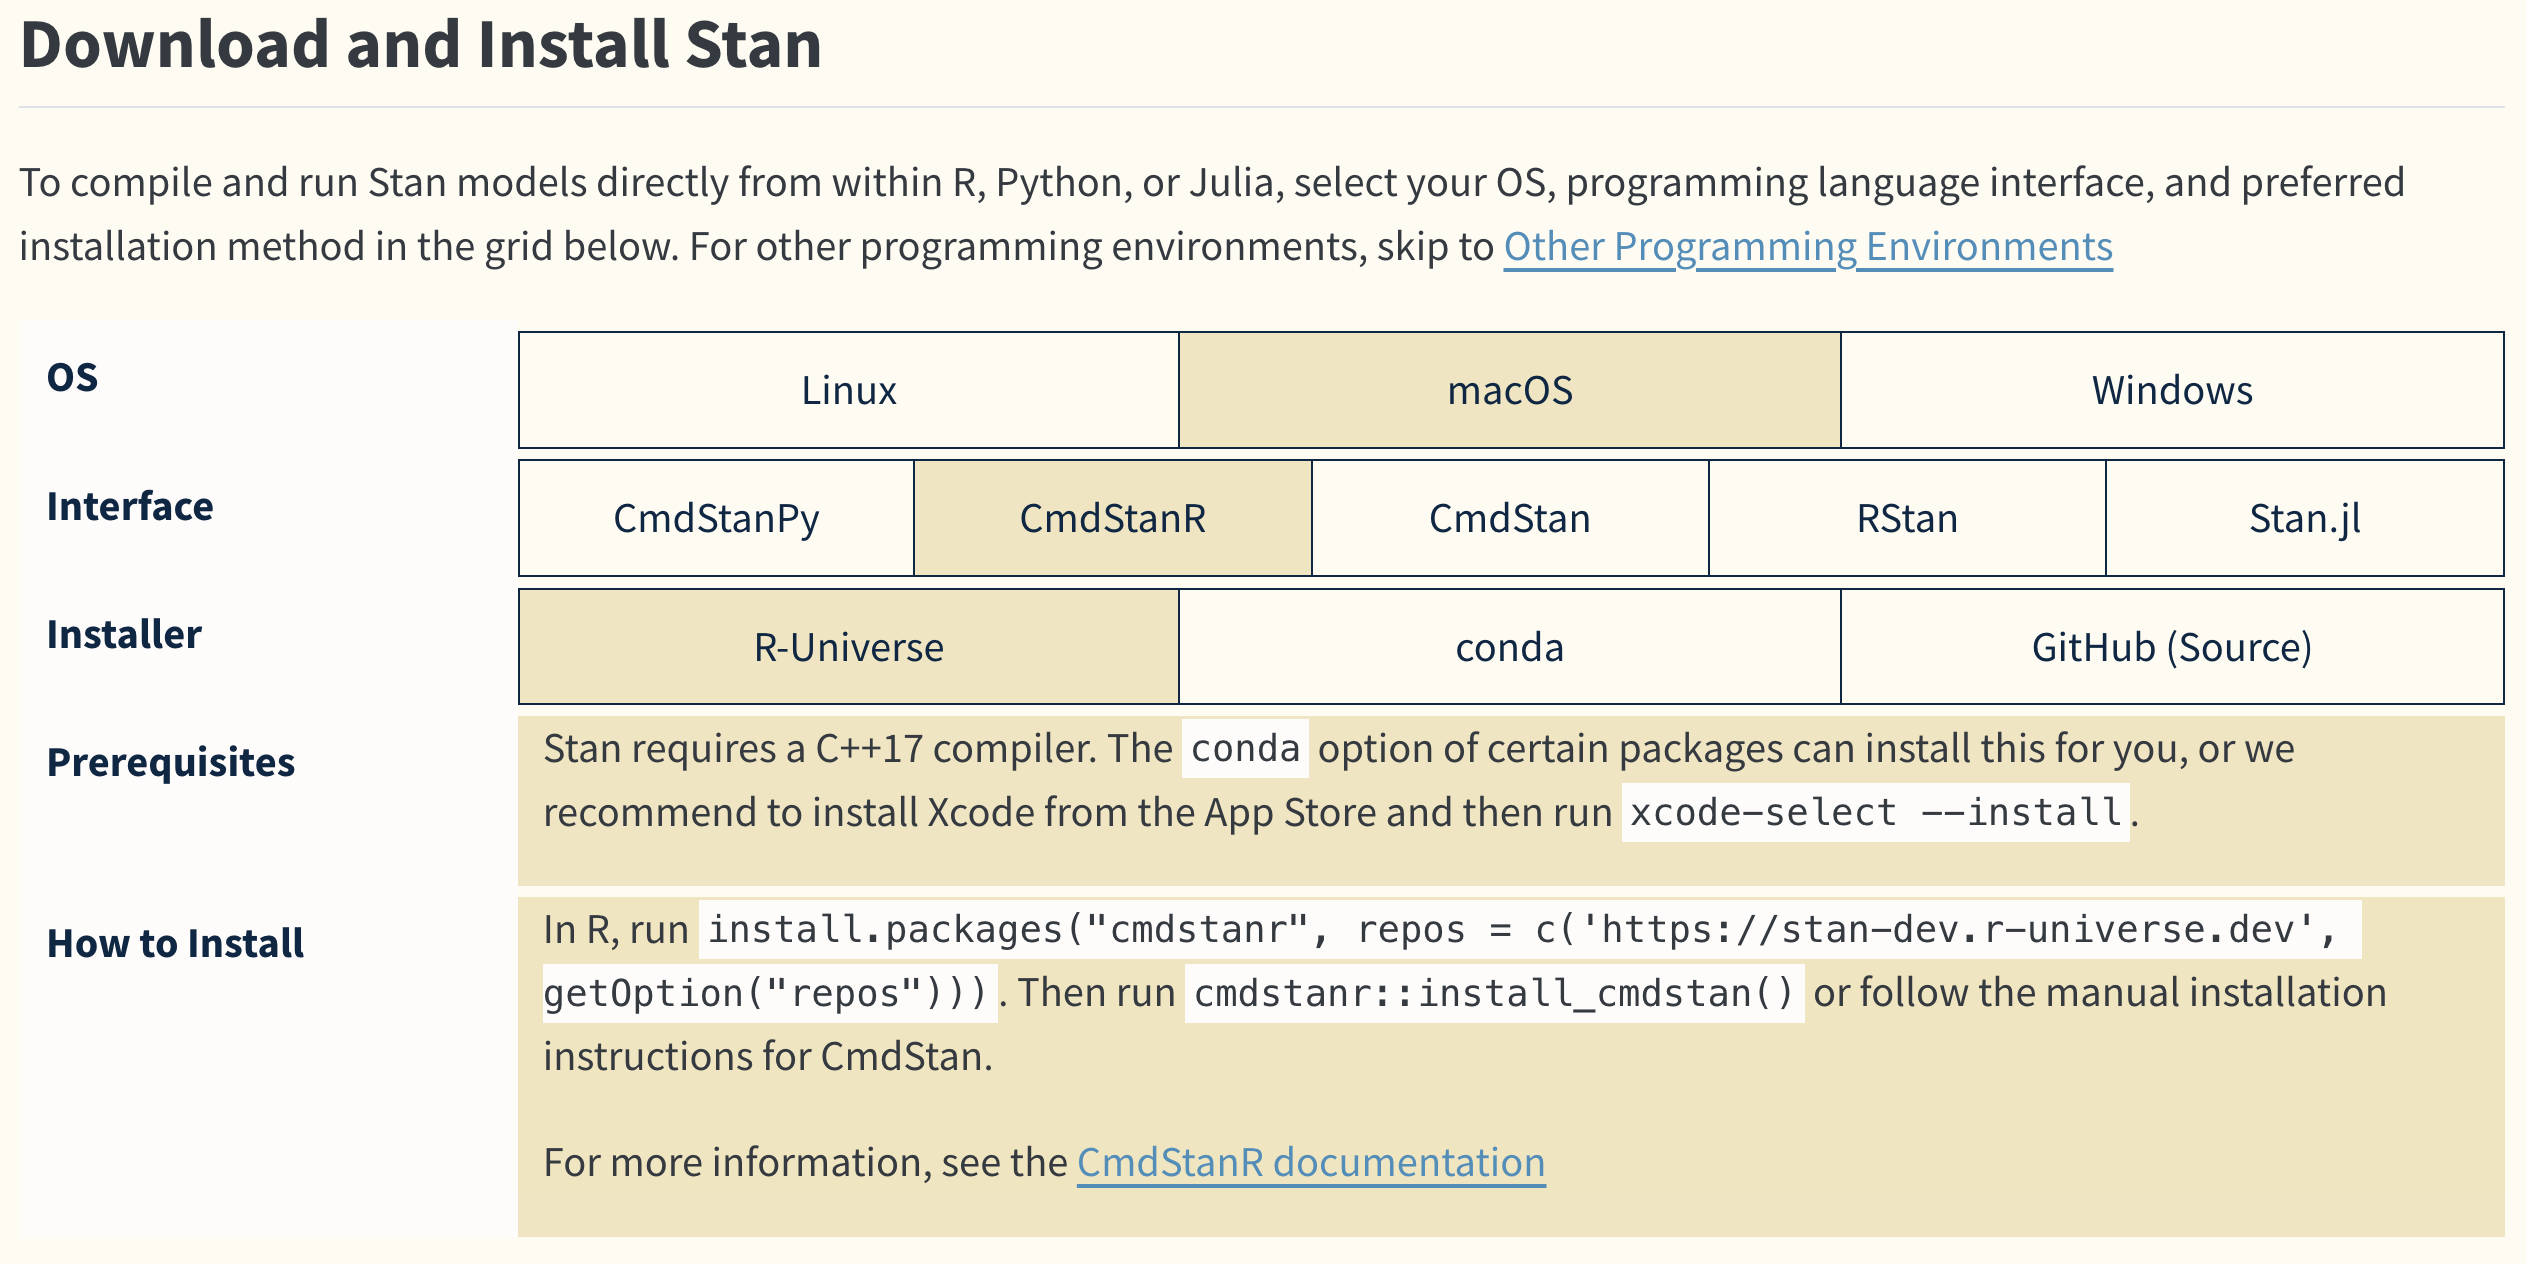
\includegraphics[keepaspectratio]{images/12_stan_install.png}}

画面ではOSとしてMacOSを選んでいるが,ここは各自の環境に合わせてもらいたい。インターフェイスは\texttt{CmdStanR}を選択して欲しい。Stanを実行するにはCコンパイラが必要であり,また\texttt{CmdStanR}はコマンドラインからStanを実行してRに繋げるという代物で,\texttt{cmdstanr::install\_cmdstan}関数を実行した後,インストール先のパスを設定する必要がある。

\texttt{CmdStanR}はstan言語で書いた確率モデルを実行し,計算機内部で事後分布を作ってその代表値(MCMCサンプル)を出力させることができる。自ら確率モデルを書くことができるので自由度が高いが,線形モデルに限定して実行するのであれば,Stanを開発しているのと同じチームが提供する\texttt{brms}パッケージが便利である。

\texttt{brms}パッケージを用いれば,Rの\texttt{formula}の指定の仕方で一般化混合線形モデル,階層線形モデルなどが表現できる。これらの非ベイズ推定版である\texttt{lmer}パッケージとその書式が同じなので,非常に使いやすい。このパッケージの導入は,一般的な\texttt{CRAN}からのインストールでも可能である。詳しくは\href{https://github.com/paul-buerkner/brms}{brmsのサイト}を参照してほしい。

\begin{Shaded}
\begin{Highlighting}[]
\FunctionTok{install.packages}\NormalTok{(}\StringTok{"brms"}\NormalTok{)}
\end{Highlighting}
\end{Shaded}

これらの環境の準備ができたものとして,使い方を見ていこう。

\section{ベイズ法による推定の例}\label{ux30d9ux30a4ux30baux6cd5ux306bux3088ux308bux63a8ux5b9aux306eux4f8b}

\subsection{パラメータリカバリによる確認と結果の読み取り}\label{ux30d1ux30e9ux30e1ux30fcux30bfux30eaux30abux30d0ux30eaux306bux3088ux308bux78baux8a8dux3068ux7d50ux679cux306eux8aadux307fux53d6ux308a}

前回に倣って,回帰分析のモデル式にそってデータを生成し,分析によってパラメータリカバリを行ってみよう。

説明変数については制約がないので一様乱数から生成し,平均0,標準偏差\(\sigma\)の誤差とともに被説明変数を作り,従来のやり方で推定してみよう。

\begin{Shaded}
\begin{Highlighting}[]
\NormalTok{pacman}\SpecialCharTok{::}\FunctionTok{p\_load}\NormalTok{(tidyverse)}
\FunctionTok{set.seed}\NormalTok{(}\DecValTok{123}\NormalTok{)}
\NormalTok{n }\OtherTok{\textless{}{-}} \DecValTok{500}
\NormalTok{beta0 }\OtherTok{\textless{}{-}} \DecValTok{2}
\NormalTok{beta1 }\OtherTok{\textless{}{-}} \DecValTok{3}
\NormalTok{sigma }\OtherTok{\textless{}{-}} \DecValTok{1}
\CommentTok{\# データの生成}
\NormalTok{x }\OtherTok{\textless{}{-}} \FunctionTok{runif}\NormalTok{(n, }\SpecialCharTok{{-}}\DecValTok{10}\NormalTok{, }\DecValTok{10}\NormalTok{)}
\NormalTok{e }\OtherTok{\textless{}{-}} \FunctionTok{rnorm}\NormalTok{(n, }\DecValTok{0}\NormalTok{, sigma)}
\NormalTok{y }\OtherTok{\textless{}{-}}\NormalTok{ beta0 }\SpecialCharTok{+}\NormalTok{ beta1 }\SpecialCharTok{*}\NormalTok{ x }\SpecialCharTok{+}\NormalTok{ e}

\NormalTok{dat }\OtherTok{\textless{}{-}} \FunctionTok{data.frame}\NormalTok{(x, y)}
\NormalTok{result.lm }\OtherTok{\textless{}{-}} \FunctionTok{lm}\NormalTok{(y }\SpecialCharTok{\textasciitilde{}}\NormalTok{ x, }\AttributeTok{data =}\NormalTok{ dat)}
\FunctionTok{summary}\NormalTok{(result.lm)}
\end{Highlighting}
\end{Shaded}

\begin{verbatim}

Call:
lm(formula = y ~ x, data = dat)

Residuals:
     Min       1Q   Median       3Q      Max 
-2.82796 -0.61831  0.03553  0.69367  2.68062 

Coefficients:
            Estimate Std. Error t value Pr(>|t|)    
(Intercept) 2.021928   0.045010   44.92   <2e-16 ***
x           3.002194   0.007919  379.09   <2e-16 ***
---
Signif. codes:  0 '***' 0.001 '**' 0.01 '*' 0.05 '.' 0.1 ' ' 1

Residual standard error: 1.006 on 498 degrees of freedom
Multiple R-squared:  0.9965,    Adjusted R-squared:  0.9965 
F-statistic: 1.437e+05 on 1 and 498 DF,  p-value: < 2.2e-16
\end{verbatim}

結果は切片2.0219277,傾き3.0021943であるから,設定した\(\beta_0 = 2,\beta_1 = 3\)が正しく復元できた,という話であった。

これは最尤法による推定であったが,\texttt{brms}パッケージを使ってベイズ推定に変えてみよう。
方法は次のとおりである。

\begin{Shaded}
\begin{Highlighting}[]
\NormalTok{pacman}\SpecialCharTok{::}\FunctionTok{p\_load}\NormalTok{(brms)}
\NormalTok{result.bayes }\OtherTok{\textless{}{-}} \FunctionTok{brm}\NormalTok{(y }\SpecialCharTok{\textasciitilde{}}\NormalTok{ x, }\AttributeTok{data =}\NormalTok{ dat)}
\end{Highlighting}
\end{Shaded}

\begin{verbatim}
Compiling Stan program...
\end{verbatim}

\begin{verbatim}
Start sampling
\end{verbatim}

\begin{verbatim}

SAMPLING FOR MODEL 'anon_model' NOW (CHAIN 1).
Chain 1: 
Chain 1: Gradient evaluation took 1.3e-05 seconds
Chain 1: 1000 transitions using 10 leapfrog steps per transition would take 0.13 seconds.
Chain 1: Adjust your expectations accordingly!
Chain 1: 
Chain 1: 
Chain 1: Iteration:    1 / 2000 [  0%]  (Warmup)
Chain 1: Iteration:  200 / 2000 [ 10%]  (Warmup)
Chain 1: Iteration:  400 / 2000 [ 20%]  (Warmup)
Chain 1: Iteration:  600 / 2000 [ 30%]  (Warmup)
Chain 1: Iteration:  800 / 2000 [ 40%]  (Warmup)
Chain 1: Iteration: 1000 / 2000 [ 50%]  (Warmup)
Chain 1: Iteration: 1001 / 2000 [ 50%]  (Sampling)
Chain 1: Iteration: 1200 / 2000 [ 60%]  (Sampling)
Chain 1: Iteration: 1400 / 2000 [ 70%]  (Sampling)
Chain 1: Iteration: 1600 / 2000 [ 80%]  (Sampling)
Chain 1: Iteration: 1800 / 2000 [ 90%]  (Sampling)
Chain 1: Iteration: 2000 / 2000 [100%]  (Sampling)
Chain 1: 
Chain 1:  Elapsed Time: 0.012 seconds (Warm-up)
Chain 1:                0.01 seconds (Sampling)
Chain 1:                0.022 seconds (Total)
Chain 1: 

SAMPLING FOR MODEL 'anon_model' NOW (CHAIN 2).
Chain 2: 
Chain 2: Gradient evaluation took 1e-06 seconds
Chain 2: 1000 transitions using 10 leapfrog steps per transition would take 0.01 seconds.
Chain 2: Adjust your expectations accordingly!
Chain 2: 
Chain 2: 
Chain 2: Iteration:    1 / 2000 [  0%]  (Warmup)
Chain 2: Iteration:  200 / 2000 [ 10%]  (Warmup)
Chain 2: Iteration:  400 / 2000 [ 20%]  (Warmup)
Chain 2: Iteration:  600 / 2000 [ 30%]  (Warmup)
Chain 2: Iteration:  800 / 2000 [ 40%]  (Warmup)
Chain 2: Iteration: 1000 / 2000 [ 50%]  (Warmup)
Chain 2: Iteration: 1001 / 2000 [ 50%]  (Sampling)
Chain 2: Iteration: 1200 / 2000 [ 60%]  (Sampling)
Chain 2: Iteration: 1400 / 2000 [ 70%]  (Sampling)
Chain 2: Iteration: 1600 / 2000 [ 80%]  (Sampling)
Chain 2: Iteration: 1800 / 2000 [ 90%]  (Sampling)
Chain 2: Iteration: 2000 / 2000 [100%]  (Sampling)
Chain 2: 
Chain 2:  Elapsed Time: 0.012 seconds (Warm-up)
Chain 2:                0.01 seconds (Sampling)
Chain 2:                0.022 seconds (Total)
Chain 2: 

SAMPLING FOR MODEL 'anon_model' NOW (CHAIN 3).
Chain 3: 
Chain 3: Gradient evaluation took 1e-06 seconds
Chain 3: 1000 transitions using 10 leapfrog steps per transition would take 0.01 seconds.
Chain 3: Adjust your expectations accordingly!
Chain 3: 
Chain 3: 
Chain 3: Iteration:    1 / 2000 [  0%]  (Warmup)
Chain 3: Iteration:  200 / 2000 [ 10%]  (Warmup)
Chain 3: Iteration:  400 / 2000 [ 20%]  (Warmup)
Chain 3: Iteration:  600 / 2000 [ 30%]  (Warmup)
Chain 3: Iteration:  800 / 2000 [ 40%]  (Warmup)
Chain 3: Iteration: 1000 / 2000 [ 50%]  (Warmup)
Chain 3: Iteration: 1001 / 2000 [ 50%]  (Sampling)
Chain 3: Iteration: 1200 / 2000 [ 60%]  (Sampling)
Chain 3: Iteration: 1400 / 2000 [ 70%]  (Sampling)
Chain 3: Iteration: 1600 / 2000 [ 80%]  (Sampling)
Chain 3: Iteration: 1800 / 2000 [ 90%]  (Sampling)
Chain 3: Iteration: 2000 / 2000 [100%]  (Sampling)
Chain 3: 
Chain 3:  Elapsed Time: 0.011 seconds (Warm-up)
Chain 3:                0.009 seconds (Sampling)
Chain 3:                0.02 seconds (Total)
Chain 3: 

SAMPLING FOR MODEL 'anon_model' NOW (CHAIN 4).
Chain 4: 
Chain 4: Gradient evaluation took 1e-06 seconds
Chain 4: 1000 transitions using 10 leapfrog steps per transition would take 0.01 seconds.
Chain 4: Adjust your expectations accordingly!
Chain 4: 
Chain 4: 
Chain 4: Iteration:    1 / 2000 [  0%]  (Warmup)
Chain 4: Iteration:  200 / 2000 [ 10%]  (Warmup)
Chain 4: Iteration:  400 / 2000 [ 20%]  (Warmup)
Chain 4: Iteration:  600 / 2000 [ 30%]  (Warmup)
Chain 4: Iteration:  800 / 2000 [ 40%]  (Warmup)
Chain 4: Iteration: 1000 / 2000 [ 50%]  (Warmup)
Chain 4: Iteration: 1001 / 2000 [ 50%]  (Sampling)
Chain 4: Iteration: 1200 / 2000 [ 60%]  (Sampling)
Chain 4: Iteration: 1400 / 2000 [ 70%]  (Sampling)
Chain 4: Iteration: 1600 / 2000 [ 80%]  (Sampling)
Chain 4: Iteration: 1800 / 2000 [ 90%]  (Sampling)
Chain 4: Iteration: 2000 / 2000 [100%]  (Sampling)
Chain 4: 
Chain 4:  Elapsed Time: 0.011 seconds (Warm-up)
Chain 4:                0.01 seconds (Sampling)
Chain 4:                0.021 seconds (Total)
Chain 4: 
\end{verbatim}

実行に際して,\texttt{Compiling\ Stan\ program...}との文字が表示されるが,これは\texttt{brms}パッケージが内部でstan言語を書き,それをC言語に書き換えてコンパイルしていることを意味する。他にもいろいろ出力されているが解説は後述する。簡単なモデルなので,すぐにプロンプトが待機状態に戻るはずである。

さて,\texttt{summary}関数で結果の要約を見てみよう。

\begin{Shaded}
\begin{Highlighting}[]
\FunctionTok{summary}\NormalTok{(result.bayes)}
\end{Highlighting}
\end{Shaded}

\begin{verbatim}
 Family: gaussian 
  Links: mu = identity; sigma = identity 
Formula: y ~ x 
   Data: dat (Number of observations: 500) 
  Draws: 4 chains, each with iter = 2000; warmup = 1000; thin = 1;
         total post-warmup draws = 4000

Regression Coefficients:
          Estimate Est.Error l-95% CI u-95% CI Rhat Bulk_ESS Tail_ESS
Intercept     2.02      0.05     1.93     2.11 1.00     3576     2877
x             3.00      0.01     2.99     3.02 1.00     4181     2652

Further Distributional Parameters:
      Estimate Est.Error l-95% CI u-95% CI Rhat Bulk_ESS Tail_ESS
sigma     1.01      0.03     0.95     1.07 1.00     3602     2759

Draws were sampled using sampling(NUTS). For each parameter, Bulk_ESS
and Tail_ESS are effective sample size measures, and Rhat is the potential
scale reduction factor on split chains (at convergence, Rhat = 1).
\end{verbatim}

まず\texttt{Regression\ Coefficients}のところを見てみよう。とりあえずリカバリーが上手くいってるか見てみたいからだ。推定値\texttt{Estimate}のところに,2.0214066と3.0022318とあるから,なるほど正しく推定できているようである。その後に標準誤差(SE)があるのはいいとして,その次にあるのが\texttt{l-95\%CI}と\texttt{u-95\%CI},すなわちlower-upperで表される区間である。

ベイズ統計学ではわからないものを確率分布として表現する。今回わからなかったものは回帰係数だから,切片\(\beta_0\)と傾き\(\beta_1\)はそれぞれ確率として表現され,結果も確率分布(事後分布)として得られている。つまり,ここに表されているのは事後分布の95\%区間であり,\(\beta_0\)は1.9328496,
2.1114449の間に分布しているもの,という結果になっている。

最尤推定が点推定であったのに対し,ベイズ推定はこのように分布で表現されるから,表示されている推定値もその代表値である。代表値の取り方はご存知の通り,平均値,最頻値,中央値などが考えられ,そのいずれもが推定値として用いられる。平均値による代表値はExpectation
A Posteriori,EAP推定値と呼ばれる。中央値による代表値はMEDian A
Posteriori,そして最頻値というより分布のピークを取る推定値のことをMaximum
A
Posteriori,MAP推定値という。ここで得られた事後分布は分布の関数形によるものではなく,事後分布の代表値の集積による稜線で形を見ているに過ぎないから,MAP推定値を得る方法は1.ヒストグラムを書いてその最頻値である級数の平均値をとる,2.ヒストグラムにフィットする関数を近似し,そのピークを算出する,といった方法が考えられる。計算そのものはパッケージに含まれる関数を利用すれば良い。ここで大事なことは,分布の形状に応じてその代表値を選ぶことである。すなわち,正規分布のような左右対称の分布であれば,平均値,中央値,最頻値は同じ値になるが,ここが異なるようであれば歪んだ分布をしていることが考えられるから,事後分布のヒストグラムを描いて確認した上で,中央値やMAP推定値などを用いるといいだろう。

\subsection{MCMCを評価する}\label{mcmcux3092ux8a55ux4fa1ux3059ux308b}

結果はその他にもいろいろな情報を提供してくれているので,見ていこう。\texttt{summary}関数によって表示された出力の5行目,\texttt{Draws}のところにMCMCサンプリングの情報が表示されている。これによると,4つのチェインがあり,そのそれぞれが2000回反復(\texttt{iter})されたこと,そのうちの最初の1000回は\texttt{warmup}と呼ばれるステップであったこと,最後に\texttt{thin}というのがあるが,これはMCMCサンプルを間引きするためのもので,ここでは1回毎にサンプルを取っている,すなわち毎回のサンプルを用いたことがわかる。

MCMCは事後分布を作り,そこから乱数を取り出すステップであったこをと思い出そう。乱数を取り出すステップは,まず適当な初期値から始め,次に高次元同時確率空間の中である方向に移動する。その場所からまた次の場所を選ぶ,と次々とステップを進めていく形で事後分布の代表値を拾い集めてゆく。今回の例で言うと,\(\beta_0,\beta_1,\sigma\)という3つのパラメータを推定しているので3次元空間を探索する。この空間のある座標は,この3つのパラメータが取りうる可能性のある値の組み合わせである。この空間で,初期値\(t_0\)の座標に立ち,近傍の別の座標\(t_1\)に移動する。この\(t_1\)の座標も,この3つのパラメータが取りうる別の可能性の組み合わせである。同様に\(t_1\)の近傍\(t_2\),\(t_2\)の近傍\(t_3\),とステップを踏むことで,それぞれのステップがMCMCサンプルの1つとして記録されていく。この記録の集約が事後分布の近似になる。

このような形でサンプリングが進むことを考えると,まず懸念されるのが「初期値によって結果が変わるのではないか」ということである。実際,初期値によっては,サンプリングがうまくいかないことはある。うまく推定できるときは,どんな初期値から発生しても,事後分布が作る空間の密度の濃いところからサンプリングが進むので,同じような値を集めてくることができるだろう。

MCMCがうまくいってるかどうかを評価するために,MCMCでは一般的に複数の初期値から始め,別々のステップを踏んでログを取る。このステップのログをチェインと呼ぶ。つまり,それぞれのチェインは異なる初期値から始まる一連の代表値の連なりなのである。今回の結果では,4つのチェイン,つまり4つの初期値から始まったことがわかる。

さて,もう一度サンプリングの進み方を思い返してみよう。初期値から始めてステップしている最初のうちは,最終的に目的としている事後分布の代表値からは大きく外れているかもしれない。ステップを繰り返すことで,より事後分布の密度の濃いところに近づいていくのだから,最初のうちはうまくいってなくても当然である。この最初のうちのステップは代表値として信用できないので,「バーンインburn
in期間だった」ということで切り捨てることが一般的である。\texttt{brms}
が採用しているMCMCアルゴリズムのstanは,この初期の探索時に,効率よくサンプリングできるようにステップサイズ(どれぐらい遠くの近傍まで考えるか)等アルゴリズムを自動で調整する期間を設定している。これを特にウォームアップ期間という。

結果に戻ってみてみると,4つのチェインで2000ステップ(\texttt{iter})を踏んでいるが,ウォームアップ期間が1000あるので,実際にサンプリングが行われたのは1000ステップ以降である。なので\texttt{total\ post-warmup\ draws\ =4000}となっている。

\texttt{thin}は,サンプリングの間引き間隔を指定するものであった。ステップ毎に代表値のログを取っていくとしたが,原理的にはそれぞれのステップ・代表値は事後分布から独立にサンプリングされたものであるはずだ。MCMCの結果を見て,ステップ毎の自己相関を確認し,もし\(t-1\)時点の代表値が\(t\)時点の代表値に影響を与えているようであればよろしくない。そこで間引きをすることで,そのような影響を与えるようなステップを省略することで,より独立性の高いサンプルを得ることができる,と考えるのである。間引きをすると事後分布からのサンプルの数が減ることになる。また,自己相関が高いようなMCMCサンプルしか得られないのは,モデルやパラメタライゼーションが不適切である場合が多く,\texttt{thin}オプションを使うのは結果オブジェクトのサイズを減らす目的である,と考えた方がいいだろう。

推定値の出力結果に,\texttt{Rhat}と\texttt{Bulk-ESS}という指標がある。\texttt{Rhat}は,チェイン間の自己相関を表す指標で,1に近いほどよいとされる。基準として,全てのパラメータにおける\texttt{Rhat}が1.1未満であれば,複数のチェインが絡み合った,良いサンプリングであったと評価される。逆に,\texttt{Rhat}が1.1以上であれば,初期値によって異なるパラメータ空間を探索していたことになり,事後分布からの適切な代表値ではない可能性があるので,モデルの見直しなどが必要になる。\texttt{Bulk-ESS}は,有効サンプルサイズEffective
Sample
Sizeの略であり,実際に独立したサンプルが何個分の情報を持っているかを推定する指標である。これの量的目安は大まかにいって,3桁以上の数字があれば良いと言われる。逆に1,2桁の数字しか示されないのであれば,有効なサンプリングができていないと考えて,モデルの見直しなどが必要になる。

\subsection{可視化してモデルの評価をみる}\label{ux53efux8996ux5316ux3057ux3066ux30e2ux30c7ux30ebux306eux8a55ux4fa1ux3092ux307fux308b}

結果を可視化してみるとわかりやすい。次のコードは,推定されたパラメータの事後分布のヒストグラムと,トレースプロットと呼ばれるものを描画する。

\begin{Shaded}
\begin{Highlighting}[]
\FunctionTok{plot}\NormalTok{(result.bayes)}
\end{Highlighting}
\end{Shaded}

\pandocbounded{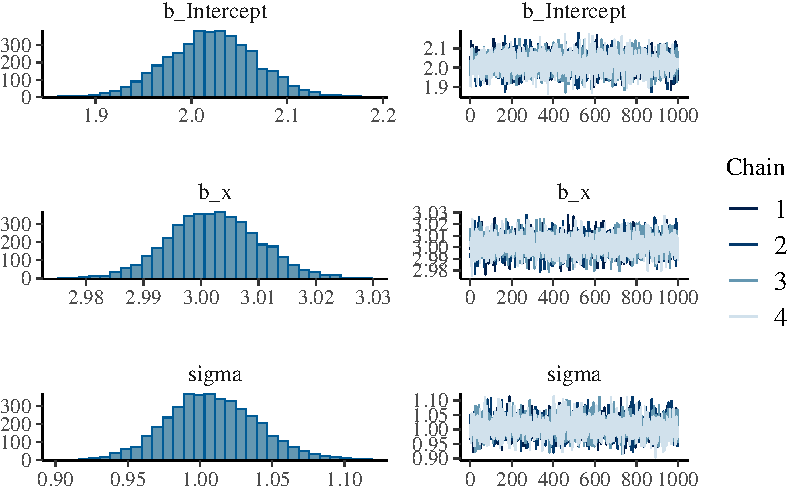
\includegraphics[keepaspectratio]{chapter12_files/figure-pdf/unnamed-chunk-5-1.pdf}}

トレースプロットとは,チェイン毎のステップログを描画したものである。チェインがうまく混合しているかどうかを確認するためのものであり,今回は4つのチェインが混じり合った状態であるから,事後分布からのサンプリングとしてはうまくいっていると考えられる。

\subsection{MCMCサンプルを確認する}\label{mcmcux30b5ux30f3ux30d7ux30ebux3092ux78baux8a8dux3059ux308b}

これら今回の出力はすでに要約されたものになっているが,具体的にどのようなMCMCサンプルが得られているか確認してみよう。結果オブジェクトから,\texttt{brms}パッケージに含まれる\texttt{as\_draws\_df}関数を用いて,MCMCサンプルをデータフレームとして取り出すことができる。

\begin{Shaded}
\begin{Highlighting}[]
\NormalTok{mcmc\_samples }\OtherTok{\textless{}{-}}\NormalTok{ brms}\SpecialCharTok{::}\FunctionTok{as\_draws\_df}\NormalTok{(result.bayes)}
\NormalTok{mcmc\_samples }\SpecialCharTok{\%\textgreater{}\%}
  \FunctionTok{as.data.frame}\NormalTok{() }\SpecialCharTok{\%\textgreater{}\%}
  \FunctionTok{head}\NormalTok{()}
\end{Highlighting}
\end{Shaded}

\begin{verbatim}
  b_Intercept      b_x     sigma Intercept    lprior      lp__ .chain
1    2.005643 3.007028 0.9670094  1.722002 -7.430387 -720.0947      1
2    2.034874 2.998960 0.9822221  1.751993 -7.430557 -719.4520      1
3    2.139143 2.994792 0.9970785  1.856656 -7.431063 -723.0209      1
4    1.997631 3.008462 1.0296125  1.713854 -7.430537 -719.7706      1
5    2.075360 3.003420 1.0175833  1.792059 -7.430834 -719.8164      1
6    2.039586 2.998572 0.9869394  1.756742 -7.430591 -719.4091      1
  .iteration .draw
1          1     1
2          2     2
3          3     3
4          4     4
5          5     5
6          6     6
\end{verbatim}

いま取り出した\texttt{mcmc\_samples}は,\texttt{as\_draws\_df}関数の出力によって,\texttt{data.frame}型の特殊系になっているので,改めて\texttt{as.data.frame}関数を用いてデータフレームに変換し,最初の数行を表示させている。
これの後ろの3列に,\texttt{.chain},\texttt{.iteration},\texttt{.draw}という列があるが,これはそれぞれMCMCサンプルのchain番号,サンプルの通し番号,サンプルの通し番号である。

すでに述べたように,デフォルトでは4つのチェインからサンプリングを行う。画面に表示されているのは,第1チェインの1,2,\ldots,6番目のステップ=サンプルである。つまり,各行が3次元同時確立空間の代表値であることを指している。

\texttt{b\_Intercept}は切片\(\beta_0\)のサンプル,\texttt{b\_x}は傾き\(\beta_1\)のサンプルである。また今回は単回帰分析であるから,\(Y \sim N(\beta_0 + \beta_1 x, \sigma)\)というモデルを推定していたわけで,\texttt{sigma}はこの\(\sigma\)のサンプルである。\texttt{Intercept}は\(\beta_0 + \beta_1 x\),すなわち正規分布の位置を表している。

\texttt{lprior}はLog
Priorの略で,パラメータの事前分布の対数を表している。\texttt{lp\_\_}はLog
Posteriorの略で,パラメータの事後分布の対数を表している。いずれも,モデルの推定に関係する情報として提供されているが,今ここは気にしなくてもいいだろう。

次のコードは,MCMCサンプルの要約統計量を使って事後分布を記述したものである。MAP推定値については,Rの\texttt{density}関数を使って,観測データからカーネル密度推定(Kernel
Density Estimation,
KDE)を計算し,そのピークの度数を取ることで,MAP推定値を算出している。

\begin{Shaded}
\begin{Highlighting}[]
\CommentTok{\# MAP推定用の関数を定義}
\NormalTok{find\_map }\OtherTok{\textless{}{-}} \ControlFlowTok{function}\NormalTok{(x) \{}
\NormalTok{  density\_obj }\OtherTok{\textless{}{-}} \FunctionTok{density}\NormalTok{(x)}
  \FunctionTok{return}\NormalTok{(density\_obj}\SpecialCharTok{$}\NormalTok{x[}\FunctionTok{which.max}\NormalTok{(density\_obj}\SpecialCharTok{$}\NormalTok{y)])}
\NormalTok{\}}

\NormalTok{mcmc\_samples }\SpecialCharTok{\%\textgreater{}\%}
  \FunctionTok{as.data.frame}\NormalTok{() }\SpecialCharTok{\%\textgreater{}\%}
  \FunctionTok{select}\NormalTok{(b\_Intercept, b\_x, sigma) }\SpecialCharTok{\%\textgreater{}\%}
  \FunctionTok{rowid\_to\_column}\NormalTok{(}\StringTok{"iter"}\NormalTok{) }\SpecialCharTok{\%\textgreater{}\%}
  \FunctionTok{pivot\_longer}\NormalTok{(}\SpecialCharTok{{-}}\NormalTok{iter) }\SpecialCharTok{\%\textgreater{}\%}
  \FunctionTok{group\_by}\NormalTok{(name) }\SpecialCharTok{\%\textgreater{}\%}
  \FunctionTok{summarise}\NormalTok{(}
    \AttributeTok{EAP =} \FunctionTok{mean}\NormalTok{(value),}
    \AttributeTok{MAD =} \FunctionTok{median}\NormalTok{(value),}
    \AttributeTok{MAP =} \FunctionTok{find\_map}\NormalTok{(value),}
    \AttributeTok{SD =} \FunctionTok{sd}\NormalTok{(value),}
    \AttributeTok{L95 =} \FunctionTok{quantile}\NormalTok{(value, }\AttributeTok{probs =} \FloatTok{0.025}\NormalTok{),}
    \AttributeTok{U95 =} \FunctionTok{quantile}\NormalTok{(value, }\AttributeTok{probs =} \FloatTok{0.975}\NormalTok{),}
    \AttributeTok{.groups =} \StringTok{"drop"}
\NormalTok{  )}
\end{Highlighting}
\end{Shaded}

\begin{verbatim}
# A tibble: 3 x 7
  name          EAP   MAD   MAP      SD   L95   U95
  <chr>       <dbl> <dbl> <dbl>   <dbl> <dbl> <dbl>
1 b_Intercept  2.02  2.02  2.02 0.0458  1.93   2.11
2 b_x          3.00  3.00  3.00 0.00786 2.99   3.02
3 sigma        1.01  1.01  1.00 0.0318  0.948  1.07
\end{verbatim}

今回は,ベイズ統計の位置付けとMCMC法によるベイズ推定の実際を,パッケージを用いて説明した。
\texttt{brms}パッケージは線形モデルやその応用において非常に強力であり,ベイズ統計の実践においては,これを用いることが多いだろう。ただし,線形モデルでないモデルについては,自分でstanのコードを書いて推定することも多い。線形モデルの限界に囚われず,自由な統計モデリングの世界があることも視野に入れておいてほしい。

\subsection{brmsパッケージのオプション}\label{brmsux30d1ux30c3ux30b1ux30fcux30b8ux306eux30aaux30d7ux30b7ux30e7ux30f3}

ベイズ推定には事前分布が必要である。しかし\texttt{brm}関数を実行した時に,事前分布は特段指定しなかった。これはパッケージがデフォルトで用意した事前分布を用いたからである。
どのような事前分布が用いられたかを確認するには,以下のようにする。

\begin{Shaded}
\begin{Highlighting}[]
\NormalTok{brms}\SpecialCharTok{::}\FunctionTok{get\_prior}\NormalTok{(result.bayes)}
\end{Highlighting}
\end{Shaded}

\begin{verbatim}
                   prior     class coef group resp dpar nlpar lb ub
                  (flat)         b                                 
                  (flat)         b    x                            
 student_t(3, 0.3, 21.3) Intercept                                 
   student_t(3, 0, 21.3)     sigma                             0   
       source
      default
 (vectorized)
      default
      default
\end{verbatim}

これをみると,回帰係数にはflatな事前分布が用いられていることがわかる。これはデータから考えられた取りうる範囲が全て等確率な,一様分布を次全部ぷとしたことを表している。これは無情報時全部分布と呼ばれる。

残差の分散\(\sigma\)については,\texttt{student\_t(3,\ 0,\ 21.3)},すなわちt分布が使われていることがわかる。具体的にこの分布がどのような形状か,描いてみてみよう。

\begin{Shaded}
\begin{Highlighting}[]
\NormalTok{df }\OtherTok{\textless{}{-}} \DecValTok{3}
\NormalTok{mu }\OtherTok{\textless{}{-}} \DecValTok{0}
\NormalTok{sigma }\OtherTok{\textless{}{-}} \FloatTok{21.3}

\FunctionTok{curve}\NormalTok{(}\DecValTok{2} \SpecialCharTok{*} \FunctionTok{dt}\NormalTok{((x }\SpecialCharTok{{-}}\NormalTok{ mu) }\SpecialCharTok{/}\NormalTok{ sigma, df) }\SpecialCharTok{/}\NormalTok{ sigma,}
  \AttributeTok{from =} \DecValTok{0}\NormalTok{, }\AttributeTok{to =} \DecValTok{100}\NormalTok{,}
  \AttributeTok{col =} \StringTok{"blue"}\NormalTok{, }\AttributeTok{lwd =} \DecValTok{2}\NormalTok{, }\AttributeTok{main =} \StringTok{"Half{-}Student{-}t Distribution"}\NormalTok{,}
  \AttributeTok{xlab =} \StringTok{"sigma"}\NormalTok{, }\AttributeTok{ylab =} \StringTok{"Density"}
\NormalTok{)}
\end{Highlighting}
\end{Shaded}

\pandocbounded{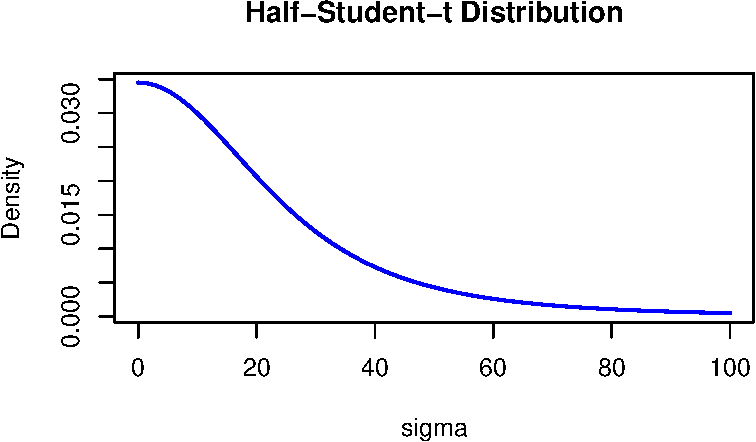
\includegraphics[keepaspectratio]{chapter12_files/figure-pdf/unnamed-chunk-8-1.pdf}}

分散は正の値しか取らないので,\texttt{brms} は
\texttt{student\_t(3,\ 0,\ 21.3)} を
半分に折りたたみ、半t分布(half-Student-t)
に変換して利用している。t分布は正規分布より裾の重い分布であり,大きな値が出る可能性も考慮されている。分散の事前分布には他にも,cauchy分布やexponential分布などが用いられることもある。

\subsection{MCMCサンプリングの設定}\label{mcmcux30b5ux30f3ux30d7ux30eaux30f3ux30b0ux306eux8a2dux5b9a}

\texttt{brms}パッケージでは,MCMCサンプリングの設定もできる。例えばチェインの数を増やすとか,warmup期間を変えるとか,間引きを変えるとか,いろいろな設定が可能である。また,再現性を確保するために乱数のシードを固定することもできる。これらの設定をしたコードの例を示す。必要に応じて,いろいろな設定を試してみるといいだろう。特に事前分布については,いろいろ変えても結果が大きく変わらない方が,推定値の信頼性も高まると考えられる。事前分布の変更によって,事後分布がどの程度影響されるかを分析することを感度分析というが,このためにも事前分布をデフォルトに任せず設定したり,デフォルトを利用したとしてもどの設定にしているのかを確認できるようになっておこう。

\begin{Shaded}
\begin{Highlighting}[]
\CommentTok{\# 事前分布の設定}
\NormalTok{priors }\OtherTok{\textless{}{-}} \FunctionTok{c}\NormalTok{(}
  \FunctionTok{set\_prior}\NormalTok{(}\StringTok{"uniform(0, 100)"}\NormalTok{, }\AttributeTok{class =} \StringTok{"Intercept"}\NormalTok{), }\CommentTok{\# 切片: 一様分布(0, 100)}
  \FunctionTok{set\_prior}\NormalTok{(}\StringTok{"normal(0, 10)"}\NormalTok{, }\AttributeTok{class =} \StringTok{"b"}\NormalTok{), }\CommentTok{\# 回帰係数: N(0, 10)}
  \FunctionTok{set\_prior}\NormalTok{(}\StringTok{"cauchy(0, 5)"}\NormalTok{, }\AttributeTok{class =} \StringTok{"sigma"}\NormalTok{) }\CommentTok{\# 標準偏差: Cauchy(0, 5)}
\NormalTok{)}

\NormalTok{fit }\OtherTok{\textless{}{-}} \FunctionTok{brm}\NormalTok{(y }\SpecialCharTok{\textasciitilde{}}\NormalTok{ x,}
  \AttributeTok{data =}\NormalTok{ dat,}
  \AttributeTok{prior =}\NormalTok{ priors,}
  \AttributeTok{iter =} \DecValTok{3000}\NormalTok{,}
  \AttributeTok{warmup =} \DecValTok{2000}\NormalTok{,}
  \AttributeTok{chains =} \DecValTok{3}\NormalTok{,}
  \AttributeTok{seed =} \DecValTok{12345}\NormalTok{,}
\NormalTok{)}
\end{Highlighting}
\end{Shaded}

\section{課題}\label{ux8ab2ux984c-10}

以下のデータセットは被説明変数\(y\),説明変数\(x1,x2\)からなる重回帰分析のサンプルデータです。データセット全体(\(n=100\))は\href{ex_regression1.csv}{ex\_regression3.csv}からダウンロード可能です。このデータセットを用いて,\texttt{brms}パッケージによる重回帰分析を実行してください。

分析結果について,以下の項目を順に報告してください:

\begin{enumerate}
\def\labelenumi{\arabic{enumi}.}
\tightlist
\item
  回帰係数(切片,\(x1\),\(x2\))の推定値と95\%信用区間
\item
  MCMCの収束診断(\texttt{Rhat}と\texttt{Bulk-ESS}の値に基づいて判断)
\item
  各パラメータの事後分布のヒストグラムとトレースプロット
\item
  デフォルトで使用された事前分布の確認と説明
\item
  MCMCサンプルからのMAP推定値の算出(本章で示した\texttt{find\_map}関数を利用)
\item
  MCMCサンプルに基づく90\%信用区間と75\%信用区間の算出
\end{enumerate}

なお,レポートには使用したRコードと,各項目の結果に対する簡潔な解釈を含めてください。

\bookmarksetup{startatroot}

\chapter{線形モデルの展開}\label{ux7ddaux5f62ux30e2ux30c7ux30ebux306eux5c55ux958b}

この章では,線形モデルの展開を説明する。線形モデルは,説明変数と目的変数の関係を線形すなわち一次式で表現するモデルである。
線形モデルは,一般化線形モデル(GLM),一般化線形混合モデル(GLMM),階層線形モデル(HLM)と拡張していくが,まずは一般線形モデル(LM)についてみておこう。

\section{一般線形モデル(General Linear
Model)}\label{ux4e00ux822cux7ddaux5f62ux30e2ux30c7ux30ebgeneral-linear-model}

線形モデルの基本は回帰分析モデルである。単回帰モデルは次の式で表される。

\[
y_i = \beta_0 + \beta_1 x + e_i
\]

ここで,\(y_i\)は\(i\)番目の観測値,\(\beta_0\)は切片,\(\beta_1\)は回帰係数,\(e_i\)は誤差項である。
この式を拡張したのが重回帰分析で,次の式で表される。

\[
y_i = \beta_0 + \beta_1 x_1 + \beta_2 x_2 + \cdots + \beta_p x_p + e_i
\]

ここで,\(x_1, x_2, \cdots, x_p\)は説明変数,\(\beta_1, \beta_2, \cdots, \beta_p\)は回帰係数である。

この式をベクトルと行列で表現すると,次のようになる。

\[
y = X\beta + e
\]

ここで,\(y\)は\(n\)次元のベクトル,\(X\)は\(n \times p\)の\textbf{計画行列}(design
matrix),\(\beta\)は\(p\)次元のベクトル,\(e\)は\(n\)次元のベクトルである。

計画行列は,説明変数のデータをまとめた行列であり,次のようになる。

\[
X = \begin{pmatrix}
1 & x_1 & x_2 & \cdots & x_p\\
1 & x_1 & x_2 & \cdots & x_p\\
\vdots & \vdots & \vdots & \ddots & \vdots\\
1 & x_1 & x_2 & \cdots & x_p
\end{pmatrix}
\]

第一列目にあるのは切片にかかる係数であり,第二列目以降にあるのは説明変数にかかる係数である。
ここに係数ベクトル\(\beta= (\beta_0, \beta_1, \beta_2, \cdots, \beta_p)^T\)をかけることで,説明変数の線形結合が得られる。

この係数ベクトルにおいて,\(x\)の値がバイナリ(0/1)の場合,その説明変数はダミー変数と呼ばれる。線型回帰モデルにおいて説明変数\(X\)がダミー変数である場合は,横軸が2つの値しかとらないため散布図を描くと奇妙な形になることがわかるだろう。

\pandocbounded{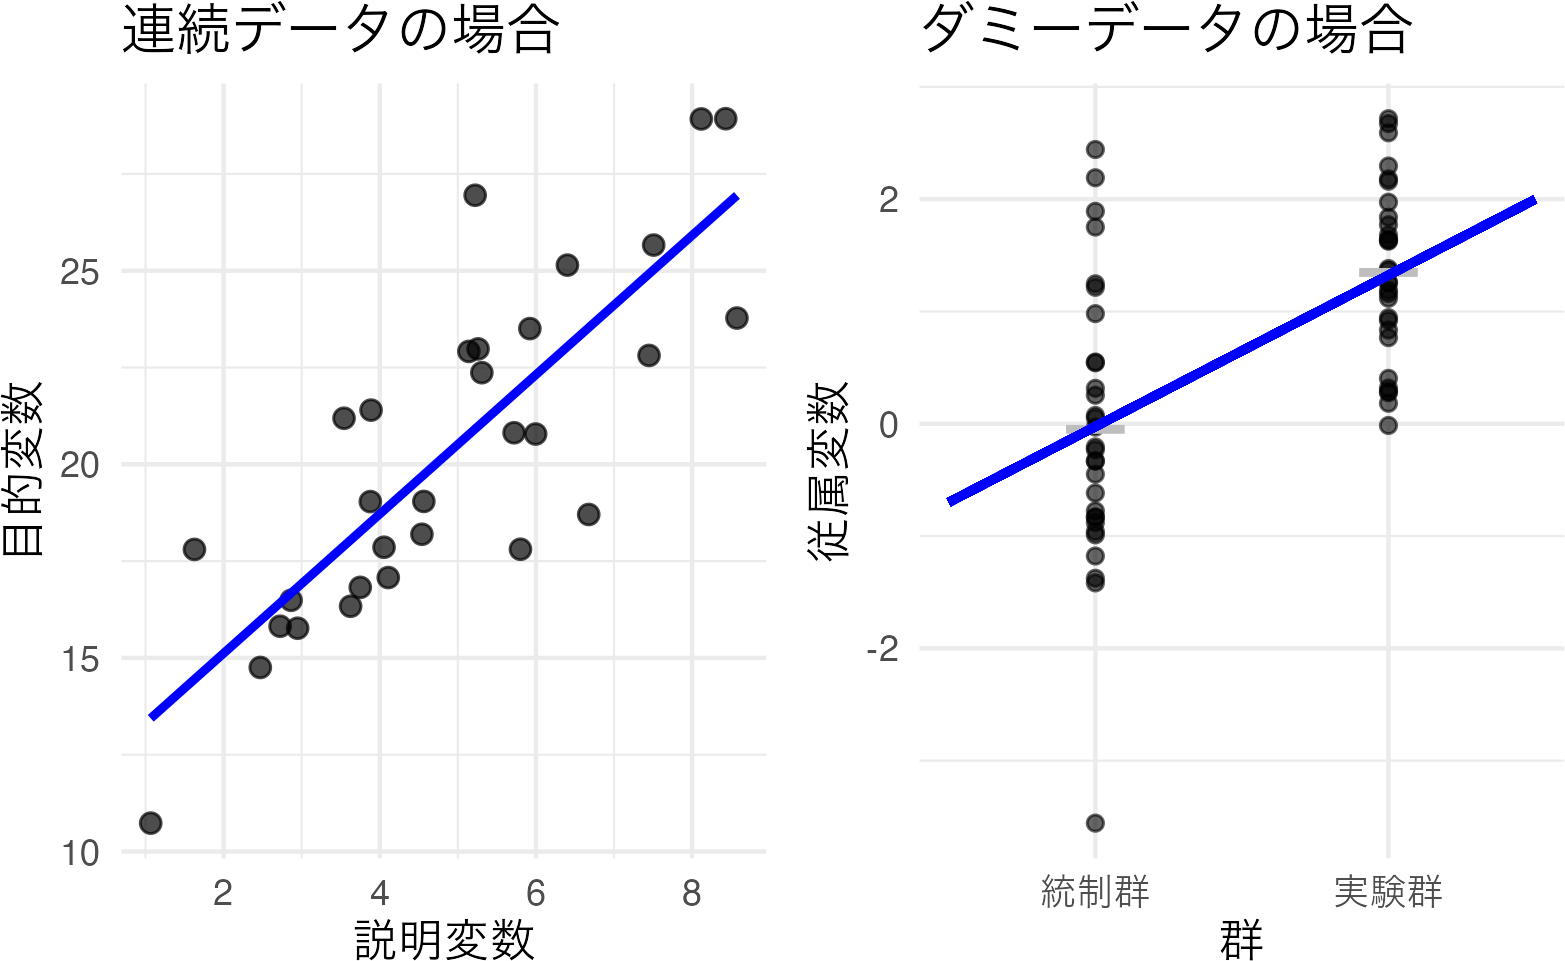
\includegraphics[keepaspectratio]{chapter13_files/figure-pdf/image_glm-1.png}}

この散布図に対して回帰直線を引けば,2群の平均値を通る直線が引かれる。回帰分析においては,予測式\(\hat{y}\)を中心とした正規分布に従って誤差が生じると仮定されているのであった。ダミーデータの場合も,両群の平均値を中心に正規分布に従って誤差が生じると仮定したことになる。これはいわゆる2群の平均値の差を検定する時の仮定と同じであり,このことから平均値差の検定は説明変数が名義尺度水準の変数である回帰分析と同じ(一般)であることがわかる。回帰分析と平均値差の検定は数学的には同じ式で表現できるから,これを総称して\textbf{一般線型モデル}General
Linear model という。

\section{一般化線形モデル(GLM)}\label{ux4e00ux822cux5316ux7ddaux5f62ux30e2ux30c7ux30ebglm}

かつて心理学実践においては,要因計画法と帰無仮説検定の組み合わせによって研究を行うことが主流であった。平均値差の検定に落とし込むように研究をデザインし,帰無仮説検定でYESかNOか決着がつく。帰無仮説検定はデータの特性や生成メカニズムに依存せず,統計パッケージを用いれば誰にでも扱うことができ,\(p\)値という手垢のついてない数値だけで判断できると考えられてきた。

このことに関する問題については置くとして,ともかく「正規分布の平均値の差」に持ち込めさえすれば良い,ということが当時の研究者の共通認識であった。そのため,例えば比率のデータやカウントデータなど,正規分布を想定することができないデータに対しても,対数変換・角変換などを行って分布を正規分布のそれに近づけ,検定を行うということが行われていた。

正規分布は理論的に\(\pm \infty\)の範囲を取るのに対し,比率のデータは0から1の範囲にしかとらない。カウントデータは正の整数しかとらないデータであるから,こうしたデータに対して一般線型モデルをあてがうのは重大な仮定違反である\footnote{エクスキューズが許されるなら,当時の統計学,計算機科学は現代に比べると貧弱で,理論的に正しくないことがわかっていても,ユーザにはそれ以上のことができなかったということがある。また心理学で測定されるデータは,あくまでも目に見えない心を表現したラフな近似値で,統計学上の仮定に違反したことで生じる問題よりも,そもそも本質的な問題があるのだから,統計の運用もあくまでもラフな近似値で良い,という風潮があったのかもしれない。}。

このような背景から,正規分布以外の確率分布を用いた統計モデルが考えられた。これが\textbf{一般化線形モデル}(Generalized
Linear Model, GLM)である\footnote{一般化線型モデルと一般線型モデルは,一文字「化」が入るかどうかの微妙な違いである。英語ではgeneralとgeneralizedの違いなので,こちらで理解した方が間違いが少なくて良いかもしれない。}。

確率分布の多くは,位置パラメータとスケールパラメータを持つ。統計モデルは平均的な挙動について考えるモデルだから,位置パラメータに線形モデルが当てがえるように,数式を変形してやれば良い。以下に例として,ベルヌーイ分布とポアソン分布をGLMで表現したものを考えてみよう。

\subsection{ベルヌーイ分布に対する線形モデル;ロジスティック回帰分析}\label{ux30d9ux30ebux30ccux30fcux30a4ux5206ux5e03ux306bux5bfeux3059ux308bux7ddaux5f62ux30e2ux30c7ux30ebux30edux30b8ux30b9ux30c6ux30a3ux30c3ux30afux56deux5e30ux5206ux6790}

ベルヌーイ分布はコイントスの表/裏のような2値をとるデータに対して用いられる。ベルヌーイ分布の確率関数は次のように表される。

\[
P(Y = y) = p^y (1-p)^{1-y}
\]

ここで,\(p\)は成功確率であり,0から1の範囲の値を取る。
こうしたデータは現実にも少なくない。生死,病気の有無,テストの正答/誤答のようなデータが代表的である。こうしたデータを目的変数にして,直線回帰を行うと当然おかしなことが生じる。すなわち,予測値が0と1の範囲を超えることがありえるからである。

そこで,線形予測子と確率を適切に結びつけるリンク関数を用いる。ロジスティック回帰では\textbf{ロジット関数}(logit
function)をリンク関数として使用する:

\[
\text{logit}(p) = \log\left(\frac{p}{1-p}\right) = \beta_0 + \beta_1 x
\]

この関係を\(p\)について解いてみよう。\(\eta = \beta_0 + \beta_1 x\)とおくと:

\[
\log\left(\frac{p}{1-p}\right) = \eta
\]

両辺の指数を取ると:

\[
\frac{p}{1-p} = e^{\eta}
\]

両辺に\((1-p)\)をかけると:

\[
p = (1-p) \cdot e^{\eta}
\]

展開すると:

\[
p = e^{\eta} - p \cdot e^{\eta}
\]

\(p\)について整理すると:

\[
p + p \cdot e^{\eta} = e^{\eta}
\]

\[
p(1 + e^{\eta}) = e^{\eta}
\]

\[
p = \frac{e^{\eta}}{1 + e^{\eta}}
\]

分子分母を\(e^{\eta}\)で割ると:

\[
p = \frac{1}{e^{-\eta} + 1} = \frac{1}{1 + e^{-\eta}}
\]

\(\eta = \beta_0 + \beta_1 x\)を代入すると,\textbf{ロジスティック関数}(逆リンク関数)が得られる:

\[
p = \frac{1}{1 + e^{-(\beta_0 + \beta_1 x)}}
\]

このようにして得られた確率を用いて,ベルヌーイ分布の確率関数を次のように表現できる。

\[ y \sim \text{Bernoulli}(p) \]

サンプルデータを作って,線形回帰モデルとロジスティック回帰モデルの予測値を比較してみよう。

\begin{Shaded}
\begin{Highlighting}[]
\NormalTok{pacman}\SpecialCharTok{::}\FunctionTok{p\_load}\NormalTok{(tidyverse)}
\NormalTok{pacman}\SpecialCharTok{::}\FunctionTok{p\_load}\NormalTok{(patchwork)}

\CommentTok{\# データ生成}
\FunctionTok{set.seed}\NormalTok{(}\DecValTok{17}\NormalTok{)}
\NormalTok{n }\OtherTok{\textless{}{-}} \DecValTok{200}
\NormalTok{x }\OtherTok{\textless{}{-}} \FunctionTok{runif}\NormalTok{(n, }\AttributeTok{min =} \SpecialCharTok{{-}}\DecValTok{10}\NormalTok{, }\AttributeTok{max =} \DecValTok{10}\NormalTok{)}
\NormalTok{beta\_0 }\OtherTok{\textless{}{-}} \DecValTok{1}
\NormalTok{beta\_1 }\OtherTok{\textless{}{-}} \DecValTok{2}
\NormalTok{p }\OtherTok{\textless{}{-}}\NormalTok{ beta\_0 }\SpecialCharTok{+}\NormalTok{ x }\SpecialCharTok{*}\NormalTok{ beta\_1}
\NormalTok{prob }\OtherTok{\textless{}{-}} \DecValTok{1}\SpecialCharTok{/}\NormalTok{(}\DecValTok{1}\SpecialCharTok{+}\FunctionTok{exp}\NormalTok{(}\SpecialCharTok{{-}}\NormalTok{p))}
\NormalTok{y }\OtherTok{\textless{}{-}} \FunctionTok{rbinom}\NormalTok{(n, }\AttributeTok{size =} \DecValTok{1}\NormalTok{, }\AttributeTok{prob =}\NormalTok{ prob)}

\NormalTok{df\_logistic }\OtherTok{\textless{}{-}} \FunctionTok{data.frame}\NormalTok{(}\AttributeTok{x =}\NormalTok{ x, }\AttributeTok{y =}\NormalTok{ y)}

\CommentTok{\# p1: 線形回帰}
\NormalTok{p1 }\OtherTok{\textless{}{-}} \FunctionTok{ggplot}\NormalTok{(df\_logistic, }\FunctionTok{aes}\NormalTok{(}\AttributeTok{x =}\NormalTok{ x, }\AttributeTok{y =}\NormalTok{ y)) }\SpecialCharTok{+}
    \FunctionTok{geom\_point}\NormalTok{(}\AttributeTok{alpha =} \FloatTok{0.7}\NormalTok{, }\AttributeTok{size =} \DecValTok{2}\NormalTok{) }\SpecialCharTok{+}
    \FunctionTok{geom\_smooth}\NormalTok{(}\AttributeTok{method =} \StringTok{"lm"}\NormalTok{, }\AttributeTok{se =} \ConstantTok{FALSE}\NormalTok{, }\AttributeTok{color =} \StringTok{"blue"}\NormalTok{) }\SpecialCharTok{+}
    \FunctionTok{theme\_minimal}\NormalTok{() }\SpecialCharTok{+}
    \FunctionTok{labs}\NormalTok{(}\AttributeTok{x =} \StringTok{"説明変数"}\NormalTok{, }\AttributeTok{y =} \StringTok{"目的変数"}\NormalTok{, }\AttributeTok{title =} \StringTok{"線形回帰"}\NormalTok{) }\SpecialCharTok{+}
    \FunctionTok{theme}\NormalTok{(}\AttributeTok{text =} \FunctionTok{element\_text}\NormalTok{(}\AttributeTok{family =} \StringTok{"IPAexGothic"}\NormalTok{))}

\CommentTok{\# p2: ロジスティック回帰}
\NormalTok{p2 }\OtherTok{\textless{}{-}} \FunctionTok{ggplot}\NormalTok{(df\_logistic, }\FunctionTok{aes}\NormalTok{(}\AttributeTok{x =}\NormalTok{ x, }\AttributeTok{y =}\NormalTok{ y)) }\SpecialCharTok{+}
    \FunctionTok{geom\_point}\NormalTok{(}\AttributeTok{alpha =} \FloatTok{0.7}\NormalTok{, }\AttributeTok{size =} \DecValTok{2}\NormalTok{) }\SpecialCharTok{+}
    \FunctionTok{geom\_smooth}\NormalTok{(}\AttributeTok{method =} \StringTok{"glm"}\NormalTok{, }\AttributeTok{method.args =} \FunctionTok{list}\NormalTok{(}\AttributeTok{family =} \StringTok{"binomial"}\NormalTok{), }\AttributeTok{se =} \ConstantTok{FALSE}\NormalTok{, }\AttributeTok{color =} \StringTok{"red"}\NormalTok{) }\SpecialCharTok{+}
    \FunctionTok{theme\_minimal}\NormalTok{() }\SpecialCharTok{+}
    \FunctionTok{labs}\NormalTok{(}\AttributeTok{x =} \StringTok{"説明変数"}\NormalTok{, }\AttributeTok{y =} \StringTok{"目的変数"}\NormalTok{, }\AttributeTok{title =} \StringTok{"ロジスティック回帰"}\NormalTok{) }\SpecialCharTok{+}
    \FunctionTok{theme}\NormalTok{(}\AttributeTok{text =} \FunctionTok{element\_text}\NormalTok{(}\AttributeTok{family =} \StringTok{"IPAexGothic"}\NormalTok{))}

\CommentTok{\# パッチワークで結合}
\NormalTok{p1 }\SpecialCharTok{+}\NormalTok{ p2}
\end{Highlighting}
\end{Shaded}

\pandocbounded{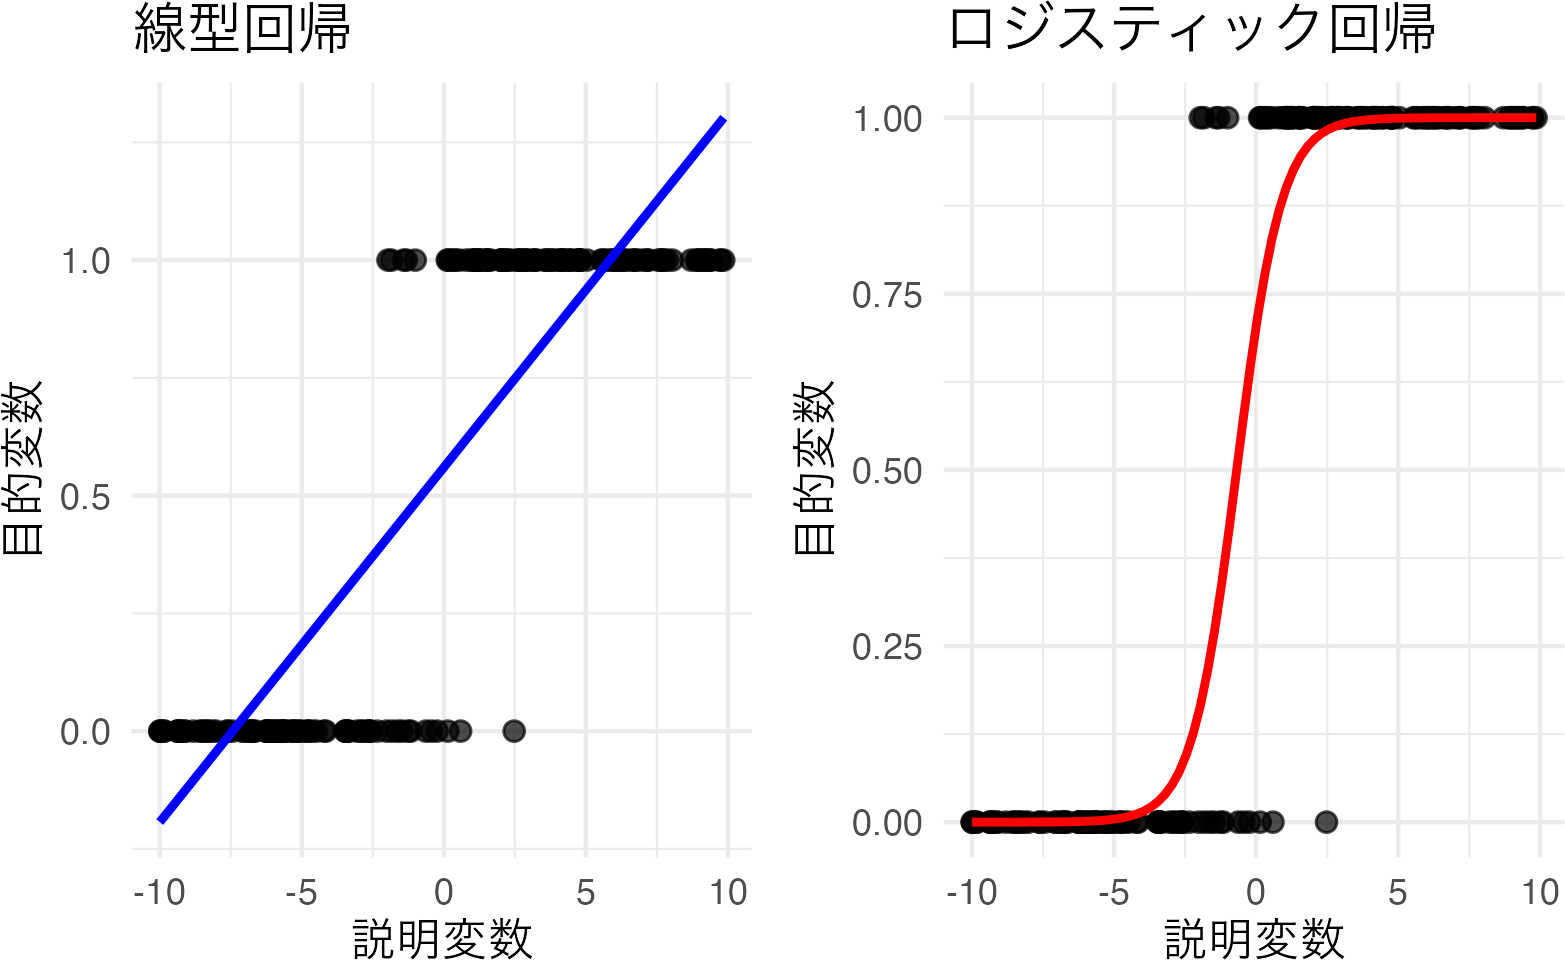
\includegraphics[keepaspectratio]{chapter13_files/figure-pdf/logistic_curve-1.png}}

線形回帰の予測値が不適切な範囲にまで延伸するのに対し,ロジスティック回帰はうまく適合していることがわかるだろう。

データからロジスティック回帰モデルを推定するには,\texttt{glm}関数を用いることができるが,ここではすでに学んだ\texttt{brms}パッケージによるベイズ推定でアプローチしてみよう。\texttt{brm}関数の書き方は,\texttt{glm}関数の書き方とほぼ同じであり,推定法をMLからベイズに変えることできる。

\begin{Shaded}
\begin{Highlighting}[]
\NormalTok{pacman}\SpecialCharTok{::}\FunctionTok{p\_load}\NormalTok{(brms)}
\NormalTok{result.bayes.logistic }\OtherTok{\textless{}{-}} \FunctionTok{brm}\NormalTok{(}
\NormalTok{    y }\SpecialCharTok{\textasciitilde{}}\NormalTok{ x,}
    \AttributeTok{family =} \FunctionTok{bernoulli}\NormalTok{(),}
    \AttributeTok{data =}\NormalTok{ df\_logistic,}
    \AttributeTok{seed =} \DecValTok{12345}\NormalTok{,}
    \AttributeTok{chains =} \DecValTok{4}\NormalTok{, }\AttributeTok{cores =} \DecValTok{4}\NormalTok{, }\AttributeTok{backend =} \StringTok{"cmdstanr"}\NormalTok{,}
    \AttributeTok{iter =} \DecValTok{2000}\NormalTok{, }\AttributeTok{warmup =} \DecValTok{1000}\NormalTok{,}
    \AttributeTok{refresh =} \DecValTok{0}
\NormalTok{)}
\end{Highlighting}
\end{Shaded}

\begin{verbatim}
Running MCMC with 4 parallel chains...

Chain 1 finished in 0.0 seconds.
Chain 2 finished in 0.0 seconds.
Chain 3 finished in 0.0 seconds.
Chain 4 finished in 0.0 seconds.

All 4 chains finished successfully.
Mean chain execution time: 0.0 seconds.
Total execution time: 0.2 seconds.
\end{verbatim}

\begin{Shaded}
\begin{Highlighting}[]
\FunctionTok{summary}\NormalTok{(result.bayes.logistic)}
\end{Highlighting}
\end{Shaded}

\begin{verbatim}
 Family: bernoulli 
  Links: mu = logit 
Formula: y ~ x 
   Data: df_logistic (Number of observations: 200) 
  Draws: 4 chains, each with iter = 2000; warmup = 1000; thin = 1;
         total post-warmup draws = 4000

Regression Coefficients:
          Estimate Est.Error l-95% CI u-95% CI Rhat Bulk_ESS Tail_ESS
Intercept     0.88      0.41     0.10     1.70 1.00     2314     2331
x             1.35      0.26     0.91     1.92 1.00     2164     2080

Draws were sampled using sample(hmc). For each parameter, Bulk_ESS
and Tail_ESS are effective sample size measures, and Rhat is the potential
scale reduction factor on split chains (at convergence, Rhat = 1).
\end{verbatim}

\begin{Shaded}
\begin{Highlighting}[]
\FunctionTok{plot}\NormalTok{(result.bayes.logistic)}
\end{Highlighting}
\end{Shaded}

\pandocbounded{\includegraphics[keepaspectratio]{chapter13_files/figure-pdf/logistic_regression-1.pdf}}

\begin{Shaded}
\begin{Highlighting}[]
\DocumentationTok{\#\# 比較のためにML推定も行っておく}
\NormalTok{result.ml }\OtherTok{\textless{}{-}} \FunctionTok{glm}\NormalTok{(y }\SpecialCharTok{\textasciitilde{}}\NormalTok{ x, }\AttributeTok{family =} \FunctionTok{binomial}\NormalTok{(), }\AttributeTok{data =}\NormalTok{ df\_logistic)}
\FunctionTok{summary}\NormalTok{(result.ml)}
\end{Highlighting}
\end{Shaded}

\begin{verbatim}

Call:
glm(formula = y ~ x, family = binomial(), data = df_logistic)

Coefficients:
            Estimate Std. Error z value Pr(>|z|)    
(Intercept)   0.8673     0.4058   2.137   0.0326 *  
x             1.2661     0.2413   5.248 1.54e-07 ***
---
Signif. codes:  0 '***' 0.001 '**' 0.01 '*' 0.05 '.' 0.1 ' ' 1

(Dispersion parameter for binomial family taken to be 1)

    Null deviance: 273.869  on 199  degrees of freedom
Residual deviance:  45.112  on 198  degrees of freedom
AIC: 49.112

Number of Fisher Scoring iterations: 8
\end{verbatim}

最尤推定の結果とベイズ推定の結果に多少のズレが見られるが,これはサンプルサイズの小ささによるものである。アウトプット変数が2値しか持たないため,分散がどうしても小さくなりがちであり,正確な推定値を得るためにはより多くのデータが必要である。

また,回帰係数の解釈には注意が必要である。普通の回帰分析であれば,説明変数が1単位変わると目的変数がどれだけ変わるかを表すが,ロジスティック回帰ではこのような直接的な解釈はできない。ロジスティック関数によって変換されたものが意味を持つからである。

線形モデルが表すのは次の関係なのであった。
\[ \beta_0 + \beta_1 x = \log \frac{p}{1-p} \]

この\(\log \frac{p}{1-p}\)は\textbf{ロジット}(logit)と呼ばれる。ロジスティック回帰では,確率\(p\)をロジットに変換することで線形関係を表現している。逆に言えば,線形モデルで表現されているのはログを取った確率の比であり,この比が説明変数の線形関係によって決まるということである。であるから,結果を解釈するには係数を指数関数\(e\)を取り,確率の比として理解する必要がある。

今回のデータでは説明変数の係数が1.36と推定されたから,\(e^{1.36} = 3.89\)である。これは,説明変数が1単位増加すると,成功確率が3.89倍になる,ということを意味する。

\subsection{ポアソン分布に対する線形モデル;ポアソン回帰}\label{ux30ddux30a2ux30bdux30f3ux5206ux5e03ux306bux5bfeux3059ux308bux7ddaux5f62ux30e2ux30c7ux30ebux30ddux30a2ux30bdux30f3ux56deux5e30}

今度はカウント変数に対するモデルを考えてみよう。カウント変数は正の整数をとるデータであり,ポアソン分布を用いることができる。ポアソン分布の確率関数は次のように表される。

\[
P(Y = y) = \frac{\lambda^y e^{-\lambda}}{y!}
\]

ここで,\(\lambda\)は平均である。ポアソン分布の形状も確認しておこう。

\pandocbounded{\includegraphics[keepaspectratio]{chapter13_files/figure-pdf/poisson_curve-1.png}}

このような正の整数しかとらないデータに対してはポアソン分布で回帰した方がよい。ポアソン回帰では\textbf{対数関数}をリンク関数として使用する:

\[
\log(\lambda_i) = \beta_0 + \beta_1 x_i
\]

この関係を\(\lambda_i\)について解くと,\textbf{指数関数}(逆リンク関数)が得られる:

\[ \lambda_i = \exp(\beta_0 + \beta_1 x_i) \]

として

\[ y_i \sim \text{Pois}(\lambda_i) \]

を考えるのである。

以下にサンプルデータを作ったポアソン回帰の例を示す。

\begin{Shaded}
\begin{Highlighting}[]
\CommentTok{\# データ生成}
\FunctionTok{set.seed}\NormalTok{(}\DecValTok{17}\NormalTok{)}
\NormalTok{n }\OtherTok{\textless{}{-}} \DecValTok{200}
\NormalTok{x }\OtherTok{\textless{}{-}} \FunctionTok{runif}\NormalTok{(n, }\AttributeTok{min =} \DecValTok{0}\NormalTok{, }\AttributeTok{max =} \DecValTok{10}\NormalTok{)}
\NormalTok{beta\_0 }\OtherTok{\textless{}{-}} \FloatTok{0.5}
\NormalTok{beta\_1 }\OtherTok{\textless{}{-}} \FloatTok{0.3}
\NormalTok{lambda }\OtherTok{\textless{}{-}} \FunctionTok{exp}\NormalTok{(beta\_0 }\SpecialCharTok{+}\NormalTok{ beta\_1 }\SpecialCharTok{*}\NormalTok{ x)}
\NormalTok{y }\OtherTok{\textless{}{-}} \FunctionTok{rpois}\NormalTok{(n, }\AttributeTok{lambda =}\NormalTok{ lambda)}

\NormalTok{df\_pois }\OtherTok{\textless{}{-}} \FunctionTok{data.frame}\NormalTok{(}\AttributeTok{x =}\NormalTok{ x, }\AttributeTok{y =}\NormalTok{ y)}

\CommentTok{\# p1: 線形回帰(不適切な例)}
\NormalTok{p1 }\OtherTok{\textless{}{-}} \FunctionTok{ggplot}\NormalTok{(df\_pois, }\FunctionTok{aes}\NormalTok{(}\AttributeTok{x =}\NormalTok{ x, }\AttributeTok{y =}\NormalTok{ y)) }\SpecialCharTok{+}
    \FunctionTok{geom\_point}\NormalTok{(}\AttributeTok{alpha =} \FloatTok{0.7}\NormalTok{, }\AttributeTok{size =} \DecValTok{2}\NormalTok{) }\SpecialCharTok{+}
    \FunctionTok{geom\_smooth}\NormalTok{(}\AttributeTok{method =} \StringTok{"lm"}\NormalTok{, }\AttributeTok{se =} \ConstantTok{FALSE}\NormalTok{, }\AttributeTok{color =} \StringTok{"blue"}\NormalTok{) }\SpecialCharTok{+}
    \FunctionTok{theme\_minimal}\NormalTok{() }\SpecialCharTok{+}
    \FunctionTok{labs}\NormalTok{(}\AttributeTok{x =} \StringTok{"説明変数"}\NormalTok{, }\AttributeTok{y =} \StringTok{"カウント変数"}\NormalTok{, }\AttributeTok{title =} \StringTok{"線形回帰(不適切)"}\NormalTok{) }\SpecialCharTok{+}
    \FunctionTok{theme}\NormalTok{(}\AttributeTok{text =} \FunctionTok{element\_text}\NormalTok{(}\AttributeTok{family =} \StringTok{"IPAexGothic"}\NormalTok{))}

\CommentTok{\# p2: ポアソン回帰(適切な例)}
\NormalTok{p2 }\OtherTok{\textless{}{-}} \FunctionTok{ggplot}\NormalTok{(df\_pois, }\FunctionTok{aes}\NormalTok{(}\AttributeTok{x =}\NormalTok{ x, }\AttributeTok{y =}\NormalTok{ y)) }\SpecialCharTok{+}
    \FunctionTok{geom\_point}\NormalTok{(}\AttributeTok{alpha =} \FloatTok{0.7}\NormalTok{, }\AttributeTok{size =} \DecValTok{2}\NormalTok{) }\SpecialCharTok{+}
    \FunctionTok{geom\_smooth}\NormalTok{(}\AttributeTok{method =} \StringTok{"glm"}\NormalTok{, }\AttributeTok{method.args =} \FunctionTok{list}\NormalTok{(}\AttributeTok{family =} \StringTok{"poisson"}\NormalTok{), }\AttributeTok{se =} \ConstantTok{FALSE}\NormalTok{, }\AttributeTok{color =} \StringTok{"red"}\NormalTok{) }\SpecialCharTok{+}
    \FunctionTok{theme\_minimal}\NormalTok{() }\SpecialCharTok{+}
    \FunctionTok{labs}\NormalTok{(}\AttributeTok{x =} \StringTok{"説明変数"}\NormalTok{, }\AttributeTok{y =} \StringTok{"カウント変数"}\NormalTok{, }\AttributeTok{title =} \StringTok{"ポアソン回帰(適切)"}\NormalTok{) }\SpecialCharTok{+}
    \FunctionTok{theme}\NormalTok{(}\AttributeTok{text =} \FunctionTok{element\_text}\NormalTok{(}\AttributeTok{family =} \StringTok{"IPAexGothic"}\NormalTok{))}

\CommentTok{\# パッチワークで結合}
\NormalTok{p1 }\SpecialCharTok{+}\NormalTok{ p2}
\end{Highlighting}
\end{Shaded}

\pandocbounded{\includegraphics[keepaspectratio]{chapter13_files/figure-pdf/poisson_plot-1.png}}

線形回帰では負の値の予測値が出てしまう可能性があるのに対し,ポアソン回帰は指数関数による変換によって適切にカウントデータの特性を捉えていることがわかる。

ポアソン回帰を実行するRコードの例を次に示す。

\begin{Shaded}
\begin{Highlighting}[]
\NormalTok{result.bayes.pois }\OtherTok{\textless{}{-}} \FunctionTok{brm}\NormalTok{(}
\NormalTok{    y }\SpecialCharTok{\textasciitilde{}}\NormalTok{ x,}
    \AttributeTok{family =} \FunctionTok{poisson}\NormalTok{(),}
    \AttributeTok{data =}\NormalTok{ df\_pois,}
    \AttributeTok{seed =} \DecValTok{12345}\NormalTok{,}
    \AttributeTok{chains =} \DecValTok{4}\NormalTok{, }\AttributeTok{cores =} \DecValTok{4}\NormalTok{, }\AttributeTok{backend =} \StringTok{"cmdstanr"}\NormalTok{,}
    \AttributeTok{iter =} \DecValTok{2000}\NormalTok{, }\AttributeTok{warmup =} \DecValTok{1000}\NormalTok{,}
    \AttributeTok{refresh =} \DecValTok{0}
\NormalTok{)}
\end{Highlighting}
\end{Shaded}

\begin{verbatim}
Running MCMC with 4 parallel chains...

Chain 1 finished in 0.0 seconds.
Chain 2 finished in 0.0 seconds.
Chain 3 finished in 0.0 seconds.
Chain 4 finished in 0.0 seconds.

All 4 chains finished successfully.
Mean chain execution time: 0.0 seconds.
Total execution time: 0.2 seconds.
\end{verbatim}

\begin{Shaded}
\begin{Highlighting}[]
\FunctionTok{summary}\NormalTok{(result.bayes.pois)}
\end{Highlighting}
\end{Shaded}

\begin{verbatim}
 Family: poisson 
  Links: mu = log 
Formula: y ~ x 
   Data: df_pois (Number of observations: 200) 
  Draws: 4 chains, each with iter = 2000; warmup = 1000; thin = 1;
         total post-warmup draws = 4000

Regression Coefficients:
          Estimate Est.Error l-95% CI u-95% CI Rhat Bulk_ESS Tail_ESS
Intercept     0.49      0.07     0.36     0.63 1.00     1275     1675
x             0.30      0.01     0.29     0.32 1.00     1471     1943

Draws were sampled using sample(hmc). For each parameter, Bulk_ESS
and Tail_ESS are effective sample size measures, and Rhat is the potential
scale reduction factor on split chains (at convergence, Rhat = 1).
\end{verbatim}

\begin{Shaded}
\begin{Highlighting}[]
\FunctionTok{plot}\NormalTok{(result.bayes.pois)}
\end{Highlighting}
\end{Shaded}

\pandocbounded{\includegraphics[keepaspectratio]{chapter13_files/figure-pdf/poisson_regression-1.pdf}}

\begin{Shaded}
\begin{Highlighting}[]
\DocumentationTok{\#\# 比較のためにML推定も行っておく}
\NormalTok{result.ml.pois }\OtherTok{\textless{}{-}} \FunctionTok{glm}\NormalTok{(y }\SpecialCharTok{\textasciitilde{}}\NormalTok{ x, }\AttributeTok{family =} \FunctionTok{poisson}\NormalTok{(), }\AttributeTok{data =}\NormalTok{ df\_pois)}
\FunctionTok{summary}\NormalTok{(result.ml.pois)}
\end{Highlighting}
\end{Shaded}

\begin{verbatim}

Call:
glm(formula = y ~ x, family = poisson(), data = df_pois)

Coefficients:
            Estimate Std. Error z value Pr(>|z|)    
(Intercept) 0.495962   0.071166   6.969 3.19e-12 ***
x           0.304829   0.009555  31.902  < 2e-16 ***
---
Signif. codes:  0 '***' 0.001 '**' 0.01 '*' 0.05 '.' 0.1 ' ' 1

(Dispersion parameter for poisson family taken to be 1)

    Null deviance: 1457.6  on 199  degrees of freedom
Residual deviance:  214.3  on 198  degrees of freedom
AIC: 975.04

Number of Fisher Scoring iterations: 4
\end{verbatim}

\section{一般化線形混合モデル(GLMM)}\label{ux4e00ux822cux5316ux7ddaux5f62ux6df7ux5408ux30e2ux30c7ux30ebglmm}

線形モデルのさらなる拡張として,\textbf{一般化線形混合モデル(GLMM)}Generalized
Linear Mixed
Modelがある。ここまでの回帰モデルは,説明変数が目的変数に対して一貫した効果を持つと仮定してきた。この効果を特に\textbf{固定効果}fixed
effectというが,GLMMでは固定効果に加えて\textbf{変量効果}random
effectを考慮することができる。

変量効果とは,説明変数が個体ごとに異なる値を持つことを意味する。たとえばWithinデザインの要因計画は個人差を考慮することができるが,これは変量効果を考慮したモデルであるといえる。すなわち,研究として見たい効果はWithin要因の水準ごとの固定効果であり,これとは別に個人の平均値が異なることを想定しているから,個人ごとの平均値を変量効果として考慮しているモデルといえる。

このように変量効果は個人ごとに異なる影響を考えることであるが,仮定としてこうした個人差が確率分布,特に正規分布に従っていると考えるのである。個人差は確率分布からランダムに生じるものであり,個人同士の平均的な違いは交換可能であると考えられる。またこうした個人差の分散は,個人の平均値の分散として捉えられる。このように個人差を表す確率分布も混ぜ込むので,混合(Mixed)モデルと呼ばれるのである。

ここでは個人差が平均値,すなわち切片が異なるものとして説明したが,傾きに対して個人差を考えることもできる。変量効果がどこにあるかによって,ランダム切片モデル,ランダム傾きモデル,ランダム切片ランダム傾きモデルなどと呼ばれることがある。

\subsection{ランダム切片モデル}\label{ux30e9ux30f3ux30c0ux30e0ux5207ux7247ux30e2ux30c7ux30eb}

ランダム切片モデルは,切片が個人ごとに異なるモデルである。切片が個人ごとに異なるということは,切片の個人差が正規分布に従うと考えることである。

\[
\beta_{0i} = \beta_0 + u_{0i}
\]

ここで,\(\beta_0\)は全体の切片,\(u_{0i}\)は個人\(i\)の切片の個人差である。個人差は正規分布に従うと考えるから,

\[
u_{0i} \sim N(0, \sigma_u)
\]

と表現できる。モデル全体としては

\[
y_{ij} = (\beta_0 + u_{0i}) + \beta_1 x_{ij} + e_{ij}
\]

となる。ここで,\(e_{ij}\)は誤差項であり,個人\(i\)の\(j\)番目の観測値に対する誤差を表す。

具体的なデータを作って見てみよう。

\begin{Shaded}
\begin{Highlighting}[]
\CommentTok{\# データ生成}
\FunctionTok{set.seed}\NormalTok{(}\DecValTok{17}\NormalTok{)}
\NormalTok{n\_person }\OtherTok{\textless{}{-}} \DecValTok{10}  \CommentTok{\# 個人数}
\NormalTok{n\_obs }\OtherTok{\textless{}{-}} \DecValTok{20}     \CommentTok{\# 各個人の観測数}
\NormalTok{beta\_0 }\OtherTok{\textless{}{-}} \DecValTok{1}
\NormalTok{beta\_1 }\OtherTok{\textless{}{-}} \DecValTok{2}
\NormalTok{sigma\_u }\OtherTok{\textless{}{-}} \DecValTok{1}    \CommentTok{\# 個人差の標準偏差}
\NormalTok{sigma\_e }\OtherTok{\textless{}{-}} \FloatTok{0.5}  \CommentTok{\# 誤差の標準偏差}

\CommentTok{\# 個人ごとのランダム切片}
\NormalTok{person\_intercepts }\OtherTok{\textless{}{-}} \FunctionTok{rnorm}\NormalTok{(n\_person, }\AttributeTok{mean =} \DecValTok{0}\NormalTok{, }\AttributeTok{sd =}\NormalTok{ sigma\_u)}

\CommentTok{\# データフレーム作成}
\NormalTok{df\_random\_intercept }\OtherTok{\textless{}{-}} \FunctionTok{expand\_grid}\NormalTok{(}
  \AttributeTok{person =} \DecValTok{1}\SpecialCharTok{:}\NormalTok{n\_person,}
  \AttributeTok{obs =} \DecValTok{1}\SpecialCharTok{:}\NormalTok{n\_obs}
\NormalTok{) }\SpecialCharTok{\%\textgreater{}\%}
  \FunctionTok{mutate}\NormalTok{(}
    \AttributeTok{x =} \FunctionTok{runif}\NormalTok{(}\FunctionTok{n}\NormalTok{(), }\AttributeTok{min =} \DecValTok{0}\NormalTok{, }\AttributeTok{max =} \DecValTok{10}\NormalTok{),}
    \AttributeTok{u\_0 =}\NormalTok{ person\_intercepts[person],}
    \AttributeTok{y =}\NormalTok{ beta\_0 }\SpecialCharTok{+}\NormalTok{ u\_0 }\SpecialCharTok{+}\NormalTok{ beta\_1 }\SpecialCharTok{*}\NormalTok{ x }\SpecialCharTok{+} \FunctionTok{rnorm}\NormalTok{(}\FunctionTok{n}\NormalTok{(), }\AttributeTok{mean =} \DecValTok{0}\NormalTok{, }\AttributeTok{sd =}\NormalTok{ sigma\_e),}
    \AttributeTok{person\_factor =} \FunctionTok{factor}\NormalTok{(person)}
\NormalTok{  )}

\DocumentationTok{\#\# データの確認}
\NormalTok{df\_random\_intercept }\SpecialCharTok{\%\textgreater{}\%} \FunctionTok{head}\NormalTok{()}
\end{Highlighting}
\end{Shaded}

\begin{verbatim}
# A tibble: 6 x 6
  person   obs     x   u_0     y person_factor
   <int> <int> <dbl> <dbl> <dbl> <fct>        
1      1     1 8.81  -1.02 17.0  1            
2      1     2 6.07  -1.02 11.5  1            
3      1     3 7.40  -1.02 15.4  1            
4      1     4 8.03  -1.02 16.9  1            
5      1     5 9.02  -1.02 18.3  1            
6      1     6 0.927 -1.02  2.00 1            
\end{verbatim}

\begin{Shaded}
\begin{Highlighting}[]
\CommentTok{\# p1: 線形回帰(全体で一つの回帰線)}
\NormalTok{p1 }\OtherTok{\textless{}{-}} \FunctionTok{ggplot}\NormalTok{(df\_random\_intercept, }\FunctionTok{aes}\NormalTok{(}\AttributeTok{x =}\NormalTok{ x, }\AttributeTok{y =}\NormalTok{ y)) }\SpecialCharTok{+}
    \FunctionTok{geom\_point}\NormalTok{(}\AttributeTok{alpha =} \FloatTok{0.5}\NormalTok{, }\AttributeTok{size =} \DecValTok{1}\NormalTok{) }\SpecialCharTok{+}
    \FunctionTok{geom\_smooth}\NormalTok{(}\AttributeTok{method =} \StringTok{"lm"}\NormalTok{, }\AttributeTok{se =} \ConstantTok{FALSE}\NormalTok{, }\AttributeTok{color =} \StringTok{"blue"}\NormalTok{, }\AttributeTok{linewidth =} \FloatTok{1.2}\NormalTok{) }\SpecialCharTok{+}
    \FunctionTok{theme\_minimal}\NormalTok{() }\SpecialCharTok{+}
    \FunctionTok{labs}\NormalTok{(}\AttributeTok{x =} \StringTok{"説明変数"}\NormalTok{, }\AttributeTok{y =} \StringTok{"目的変数"}\NormalTok{, }\AttributeTok{title =} \StringTok{"線形回帰(固定効果のみ)"}\NormalTok{) }\SpecialCharTok{+}
    \FunctionTok{theme}\NormalTok{(}\AttributeTok{text =} \FunctionTok{element\_text}\NormalTok{(}\AttributeTok{family =} \StringTok{"IPAexGothic"}\NormalTok{))}

\CommentTok{\# p2: ランダム切片モデル(個人ごとに異なる切片の回帰線)}
\NormalTok{p2 }\OtherTok{\textless{}{-}} \FunctionTok{ggplot}\NormalTok{(df\_random\_intercept, }\FunctionTok{aes}\NormalTok{(}\AttributeTok{x =}\NormalTok{ x, }\AttributeTok{y =}\NormalTok{ y, }\AttributeTok{color =}\NormalTok{ person\_factor)) }\SpecialCharTok{+}
    \FunctionTok{geom\_point}\NormalTok{(}\AttributeTok{alpha =} \FloatTok{0.6}\NormalTok{, }\AttributeTok{size =} \DecValTok{1}\NormalTok{) }\SpecialCharTok{+}
    \FunctionTok{geom\_smooth}\NormalTok{(}\AttributeTok{method =} \StringTok{"lm"}\NormalTok{, }\AttributeTok{se =} \ConstantTok{FALSE}\NormalTok{, }\AttributeTok{linewidth =} \FloatTok{0.8}\NormalTok{) }\SpecialCharTok{+}
    \FunctionTok{theme\_minimal}\NormalTok{() }\SpecialCharTok{+}
    \FunctionTok{labs}\NormalTok{(}\AttributeTok{x =} \StringTok{"説明変数"}\NormalTok{, }\AttributeTok{y =} \StringTok{"目的変数"}\NormalTok{, }\AttributeTok{title =} \StringTok{"ランダム切片モデル"}\NormalTok{) }\SpecialCharTok{+}
    \FunctionTok{theme}\NormalTok{(}
      \AttributeTok{text =} \FunctionTok{element\_text}\NormalTok{(}\AttributeTok{family =} \StringTok{"IPAexGothic"}\NormalTok{),}
      \AttributeTok{legend.position =} \StringTok{"none"}
\NormalTok{    )}

\NormalTok{p1 }\SpecialCharTok{+}\NormalTok{ p2}
\end{Highlighting}
\end{Shaded}

\pandocbounded{\includegraphics[keepaspectratio]{chapter13_files/figure-pdf/random_intercept_model plot-1.png}}

ランダム効果を含むモデルを推定するコード例を以下に示す。

\begin{Shaded}
\begin{Highlighting}[]
\NormalTok{result.bayes.random\_intercept }\OtherTok{\textless{}{-}} \FunctionTok{brm}\NormalTok{(}
\NormalTok{    y }\SpecialCharTok{\textasciitilde{}}\NormalTok{ x }\SpecialCharTok{+}\NormalTok{ (}\DecValTok{1} \SpecialCharTok{|}\NormalTok{ person),}
    \AttributeTok{family =} \FunctionTok{gaussian}\NormalTok{(),}
    \AttributeTok{data =}\NormalTok{ df\_random\_intercept,}
    \AttributeTok{seed =} \DecValTok{12345}\NormalTok{,}
    \AttributeTok{chains =} \DecValTok{4}\NormalTok{, }\AttributeTok{cores =} \DecValTok{4}\NormalTok{, }\AttributeTok{backend =} \StringTok{"cmdstanr"}\NormalTok{,}
    \AttributeTok{iter =} \DecValTok{2000}\NormalTok{, }\AttributeTok{warmup =} \DecValTok{1000}\NormalTok{,}
    \AttributeTok{refresh =} \DecValTok{0}
\NormalTok{)}
\end{Highlighting}
\end{Shaded}

\begin{verbatim}
Running MCMC with 4 parallel chains...

Chain 1 finished in 0.4 seconds.
Chain 2 finished in 0.5 seconds.
Chain 3 finished in 0.4 seconds.
Chain 4 finished in 0.5 seconds.

All 4 chains finished successfully.
Mean chain execution time: 0.4 seconds.
Total execution time: 0.6 seconds.
\end{verbatim}

\begin{Shaded}
\begin{Highlighting}[]
\FunctionTok{summary}\NormalTok{(result.bayes.random\_intercept)}
\end{Highlighting}
\end{Shaded}

\begin{verbatim}
 Family: gaussian 
  Links: mu = identity; sigma = identity 
Formula: y ~ x + (1 | person) 
   Data: df_random_intercept (Number of observations: 200) 
  Draws: 4 chains, each with iter = 2000; warmup = 1000; thin = 1;
         total post-warmup draws = 4000

Multilevel Hyperparameters:
~person (Number of levels: 10) 
              Estimate Est.Error l-95% CI u-95% CI Rhat Bulk_ESS Tail_ESS
sd(Intercept)     1.01      0.30     0.60     1.73 1.01      408      786

Regression Coefficients:
          Estimate Est.Error l-95% CI u-95% CI Rhat Bulk_ESS Tail_ESS
Intercept     1.29      0.35     0.61     2.01 1.01      620      461
x             1.98      0.01     1.96     2.01 1.00     2380     2052

Further Distributional Parameters:
      Estimate Est.Error l-95% CI u-95% CI Rhat Bulk_ESS Tail_ESS
sigma     0.53      0.03     0.48     0.59 1.00     1790     2245

Draws were sampled using sample(hmc). For each parameter, Bulk_ESS
and Tail_ESS are effective sample size measures, and Rhat is the potential
scale reduction factor on split chains (at convergence, Rhat = 1).
\end{verbatim}

\begin{Shaded}
\begin{Highlighting}[]
\FunctionTok{plot}\NormalTok{(result.bayes.random\_intercept)}
\end{Highlighting}
\end{Shaded}

\pandocbounded{\includegraphics[keepaspectratio]{chapter13_files/figure-pdf/random_intercept_model-1.pdf}}

\begin{Shaded}
\begin{Highlighting}[]
\DocumentationTok{\#\# 比較のためにML推定も行っておく}
\NormalTok{pacman}\SpecialCharTok{::}\FunctionTok{p\_load}\NormalTok{(lmerTest)}
\NormalTok{result.ml.random\_intercept }\OtherTok{\textless{}{-}} \FunctionTok{lmer}\NormalTok{(y }\SpecialCharTok{\textasciitilde{}}\NormalTok{ x }\SpecialCharTok{+}\NormalTok{ (}\DecValTok{1} \SpecialCharTok{|}\NormalTok{ person), }\AttributeTok{data =}\NormalTok{ df\_random\_intercept)}
\FunctionTok{summary}\NormalTok{(result.ml.random\_intercept)}
\end{Highlighting}
\end{Shaded}

\begin{verbatim}
Linear mixed model fit by REML. t-tests use Satterthwaite's method [
lmerModLmerTest]
Formula: y ~ x + (1 | person)
   Data: df_random_intercept

REML criterion at convergence: 356.6

Scaled residuals: 
    Min      1Q  Median      3Q     Max 
-3.3167 -0.5745 -0.1189  0.6343  2.6464 

Random effects:
 Groups   Name        Variance Std.Dev.
 person   (Intercept) 0.7462   0.8638  
 Residual             0.2773   0.5266  
Number of obs: 200, groups:  person, 10

Fixed effects:
             Estimate Std. Error        df t value Pr(>|t|)    
(Intercept)   1.26699    0.28414  10.15076   4.459  0.00117 ** 
x             1.98396    0.01361 189.35597 145.774  < 2e-16 ***
---
Signif. codes:  0 '***' 0.001 '**' 0.01 '*' 0.05 '.' 0.1 ' ' 1

Correlation of Fixed Effects:
  (Intr)
x -0.242
\end{verbatim}

\begin{Shaded}
\begin{Highlighting}[]
\DocumentationTok{\#\# さらに比較のために,普通の回帰分析も行ってみる}
\NormalTok{result.ml.random\_intercept.ordinal }\OtherTok{\textless{}{-}} \FunctionTok{lm}\NormalTok{(y }\SpecialCharTok{\textasciitilde{}}\NormalTok{ x, }\AttributeTok{data =}\NormalTok{ df\_random\_intercept)}
\FunctionTok{summary}\NormalTok{(result.ml.random\_intercept.ordinal)}
\end{Highlighting}
\end{Shaded}

\begin{verbatim}

Call:
lm(formula = y ~ x, data = df_random_intercept)

Residuals:
     Min       1Q   Median       3Q      Max 
-2.27275 -0.59838  0.08193  0.50855  2.67596 

Coefficients:
            Estimate Std. Error t value Pr(>|t|)    
(Intercept)  1.31764    0.14235   9.256   <2e-16 ***
x            1.97394    0.02464  80.124   <2e-16 ***
---
Signif. codes:  0 '***' 0.001 '**' 0.01 '*' 0.05 '.' 0.1 ' ' 1

Residual standard error: 0.9771 on 198 degrees of freedom
Multiple R-squared:  0.9701,    Adjusted R-squared:  0.9699 
F-statistic:  6420 on 1 and 198 DF,  p-value: < 2.2e-16
\end{verbatim}

変量効果のモデル表記は,固定効果に加えて\texttt{(1\ \textbar{}\ person)}のように表記する。ここで,\texttt{1}は切片を表し,\texttt{person}は個人を表す。このようにすることで,個人ごとに異なる切片を考慮することができる。

設定したパラメタ(個人差の標準偏差\(\sigma_u\) =
1,残差の標準偏差\(\sigma_e\) =
0.5)に対して,ベイズ推定では個人差の標準偏差が1.012,残差の標準偏差が0.53と推定されている。ML推定では個人差の標準偏差が0.864,残差の標準偏差が0.527と推定された。両手法ともに設定値に近い値が得られており,適切にパラメタが推定されていることがわかる。

このデータに対して,固定効果のみで推定すると切片が1.318,傾きが1.974と推定される。傾きに対しては同じ値になるが切片の変動を考慮するかどうかで推定値が異なっていることがわかる。固定効果のみのモデルの場合,切片に想定された正規分布の平均値のみ推定したことになっている。実践的な意味としては,Within計画をBetween計画と皆して推定しているようなものであり,せっかく綺麗に取り分けられる個人差分散を無視しているようなものである。

\subsubsection{個人レベルの推定値の取得}\label{ux500bux4ebaux30ecux30d9ux30ebux306eux63a8ux5b9aux5024ux306eux53d6ux5f97}

ベイズ推定の利点の一つは,個人ごとの推定値とその不確実性を定量化できることである。MCMCサンプルから個人の変量効果を取り出し,事後分布を可視化してみよう。

\texttt{brms}パッケージの関数\texttt{ranef}を使うと面倒なことをしなくても直接取り出してくれるが,MCMCサンプルを取り出して加工して確認することは,MCMCによる推定の理解を深めるのに良い訓練となる。

\begin{Shaded}
\begin{Highlighting}[]
\CommentTok{\# 個人ごとの変量効果を取得して表示してみる}
\NormalTok{random\_effects }\OtherTok{\textless{}{-}} \FunctionTok{ranef}\NormalTok{(result.bayes.random\_intercept)}
\FunctionTok{print}\NormalTok{(random\_effects)}
\end{Highlighting}
\end{Shaded}

\begin{verbatim}
$person
, , Intercept

     Estimate Est.Error       Q2.5      Q97.5
1  -1.2842574 0.3604082 -2.0328445 -0.6093264
2  -0.2815002 0.3612608 -1.0005500  0.4143775
3  -0.4328320 0.3614323 -1.1734005  0.2534434
4  -1.0881607 0.3642191 -1.8473405 -0.4056347
5   0.5388313 0.3636371 -0.2012679  1.2376413
6  -0.2689177 0.3633187 -1.0316235  0.4175829
7   0.5917789 0.3634518 -0.1563293  1.3063205
8   1.6501281 0.3597518  0.9219949  2.3568723
9   0.1666085 0.3624218 -0.5813912  0.8600216
10  0.2276495 0.3628401 -0.5134040  0.9184448
\end{verbatim}

\begin{Shaded}
\begin{Highlighting}[]
\CommentTok{\# 個人の切片の変量効果の事後分布(MCMCサンプル)を取得}
\NormalTok{posterior\_samples }\OtherTok{\textless{}{-}} \FunctionTok{as\_draws\_df}\NormalTok{(result.bayes.random\_intercept) }\SpecialCharTok{\%\textgreater{}\%} 
  \FunctionTok{select}\NormalTok{(}\FunctionTok{starts\_with}\NormalTok{(}\StringTok{"r\_person"}\NormalTok{)) }\SpecialCharTok{\%\textgreater{}\%} 
  \FunctionTok{rowid\_to\_column}\NormalTok{(}\StringTok{"iter"}\NormalTok{) }\SpecialCharTok{\%\textgreater{}\%} 
  \FunctionTok{pivot\_longer}\NormalTok{(}\SpecialCharTok{{-}}\NormalTok{iter) }\SpecialCharTok{\%\textgreater{}\%} 
  \FunctionTok{mutate}\NormalTok{(}\AttributeTok{person =} \FunctionTok{str\_extract}\NormalTok{(name,}\AttributeTok{pattern=}\StringTok{"}\SpecialCharTok{\textbackslash{}\textbackslash{}}\StringTok{d+"}\NormalTok{)) }\SpecialCharTok{\%\textgreater{}\%} 
  \FunctionTok{mutate}\NormalTok{(}\AttributeTok{person =} \FunctionTok{factor}\NormalTok{(person, }\AttributeTok{levels =} \FunctionTok{as.character}\NormalTok{(}\DecValTok{1}\SpecialCharTok{:}\DecValTok{10}\NormalTok{))) }\SpecialCharTok{\%\textgreater{}\%} 
  \FunctionTok{select}\NormalTok{(}\SpecialCharTok{{-}}\NormalTok{name)}
\end{Highlighting}
\end{Shaded}

\begin{verbatim}
Warning: Dropping 'draws_df' class as required metadata was removed.
\end{verbatim}

\begin{Shaded}
\begin{Highlighting}[]
\CommentTok{\# MCMCサンプルを使った要約}
\NormalTok{posterior\_samples }\SpecialCharTok{\%\textgreater{}\%} 
  \FunctionTok{group\_by}\NormalTok{(person) }\SpecialCharTok{\%\textgreater{}\%} 
  \FunctionTok{summarise}\NormalTok{(}
    \AttributeTok{EAP =} \FunctionTok{mean}\NormalTok{(value),}
    \AttributeTok{median =} \FunctionTok{quantile}\NormalTok{(value, }\FloatTok{0.5}\NormalTok{),}
    \AttributeTok{q025 =} \FunctionTok{quantile}\NormalTok{(value, }\FloatTok{0.025}\NormalTok{),}
    \AttributeTok{q975 =} \FunctionTok{quantile}\NormalTok{(value, }\FloatTok{0.975}\NormalTok{),}
    \AttributeTok{sd =} \FunctionTok{sd}\NormalTok{(value),}
    \AttributeTok{.groups =} \StringTok{"drop"}
\NormalTok{  )}
\end{Highlighting}
\end{Shaded}

\begin{verbatim}
# A tibble: 10 x 6
   person    EAP median   q025   q975    sd
   <fct>   <dbl>  <dbl>  <dbl>  <dbl> <dbl>
 1 1      -1.28  -1.28  -2.03  -0.609 0.360
 2 2      -0.282 -0.273 -1.00   0.414 0.361
 3 3      -0.433 -0.425 -1.17   0.253 0.361
 4 4      -1.09  -1.08  -1.85  -0.406 0.364
 5 5       0.539  0.545 -0.201  1.24  0.364
 6 6      -0.269 -0.270 -1.03   0.418 0.363
 7 7       0.592  0.593 -0.156  1.31  0.363
 8 8       1.65   1.66   0.922  2.36  0.360
 9 9       0.167  0.171 -0.581  0.860 0.362
10 10      0.228  0.235 -0.513  0.918 0.363
\end{verbatim}

\begin{Shaded}
\begin{Highlighting}[]
\CommentTok{\# 事後分布の描画}
\NormalTok{p1 }\OtherTok{\textless{}{-}} \FunctionTok{ggplot}\NormalTok{(posterior\_samples, }\FunctionTok{aes}\NormalTok{(}\AttributeTok{x =}\NormalTok{ value, }\AttributeTok{fill =}\NormalTok{ person)) }\SpecialCharTok{+}
  \FunctionTok{geom\_density}\NormalTok{(}\AttributeTok{alpha =} \FloatTok{0.7}\NormalTok{) }\SpecialCharTok{+}
  \FunctionTok{facet\_wrap}\NormalTok{(}\SpecialCharTok{\textasciitilde{}}\NormalTok{ person, }\AttributeTok{scales =} \StringTok{"free\_y"}\NormalTok{) }\SpecialCharTok{+}
  \FunctionTok{theme\_minimal}\NormalTok{() }\SpecialCharTok{+}
  \FunctionTok{labs}\NormalTok{(}\AttributeTok{x =} \StringTok{"切片の変量効果"}\NormalTok{, }\AttributeTok{y =} \StringTok{"事後密度"}\NormalTok{, }\AttributeTok{title =} \StringTok{"個人ごとの切片変量効果の事後分布"}\NormalTok{) }\SpecialCharTok{+}
  \FunctionTok{theme}\NormalTok{(}\AttributeTok{text =} \FunctionTok{element\_text}\NormalTok{(}\AttributeTok{family =} \StringTok{"IPAexGothic"}\NormalTok{), }\AttributeTok{legend.position =} \StringTok{"none"}\NormalTok{)}

\FunctionTok{print}\NormalTok{(p1)}
\end{Highlighting}
\end{Shaded}

\pandocbounded{\includegraphics[keepaspectratio]{chapter13_files/figure-pdf/individual_estimates-1.png}}

ここで抜き出された個人の効果は,全体平均からの偏差であり,実際の切片は固定効果+変量効果の形で得られている。これについても\texttt{coef}関数あるいはMCMCサンプルを加工することで,より具体的にイメージしながら利用できるだろう。

\begin{Shaded}
\begin{Highlighting}[]
\CommentTok{\# 各個人の実際の切片(固定効果+変量効果)を取得}
\NormalTok{individual\_coefs }\OtherTok{\textless{}{-}} \FunctionTok{coef}\NormalTok{(result.bayes.random\_intercept)}\SpecialCharTok{$}\NormalTok{person}

\CommentTok{\# 実際の切片の事後分布(固定効果+変量効果)}
\NormalTok{total\_intercept\_samples }\OtherTok{\textless{}{-}} \FunctionTok{as\_draws\_df}\NormalTok{(result.bayes.random\_intercept) }\SpecialCharTok{\%\textgreater{}\%} 
  \FunctionTok{select}\NormalTok{(b\_Intercept, }\FunctionTok{starts\_with}\NormalTok{(}\StringTok{"r\_person"}\NormalTok{)) }\SpecialCharTok{\%\textgreater{}\%} 
  \FunctionTok{rowid\_to\_column}\NormalTok{(}\StringTok{"iter"}\NormalTok{) }\SpecialCharTok{\%\textgreater{}\%} 
  \FunctionTok{pivot\_longer}\NormalTok{(}\SpecialCharTok{{-}}\FunctionTok{c}\NormalTok{(iter, b\_Intercept)) }\SpecialCharTok{\%\textgreater{}\%} 
  \FunctionTok{mutate}\NormalTok{(}\AttributeTok{person =} \FunctionTok{str\_extract}\NormalTok{(name, }\AttributeTok{pattern=}\StringTok{"}\SpecialCharTok{\textbackslash{}\textbackslash{}}\StringTok{d+"}\NormalTok{)) }\SpecialCharTok{\%\textgreater{}\%} 
  \FunctionTok{mutate}\NormalTok{(}\AttributeTok{person =} \FunctionTok{factor}\NormalTok{(person, }\AttributeTok{levels =} \FunctionTok{as.character}\NormalTok{(}\DecValTok{1}\SpecialCharTok{:}\DecValTok{10}\NormalTok{))) }\SpecialCharTok{\%\textgreater{}\%} 
  \FunctionTok{mutate}\NormalTok{(}\AttributeTok{total\_intercept =}\NormalTok{ b\_Intercept }\SpecialCharTok{+}\NormalTok{ value) }\SpecialCharTok{\%\textgreater{}\%} 
  \FunctionTok{select}\NormalTok{(iter, person, total\_intercept)}
\end{Highlighting}
\end{Shaded}

\begin{verbatim}
Warning: Dropping 'draws_df' class as required metadata was removed.
\end{verbatim}

\begin{Shaded}
\begin{Highlighting}[]
\CommentTok{\# 実際の切片の事後分布の描画}
\NormalTok{p2 }\OtherTok{\textless{}{-}} \FunctionTok{ggplot}\NormalTok{(total\_intercept\_samples, }\FunctionTok{aes}\NormalTok{(}\AttributeTok{x =}\NormalTok{ total\_intercept, }\AttributeTok{fill =}\NormalTok{ person)) }\SpecialCharTok{+}
  \FunctionTok{geom\_density}\NormalTok{(}\AttributeTok{alpha =} \FloatTok{0.7}\NormalTok{) }\SpecialCharTok{+}
  \FunctionTok{facet\_wrap}\NormalTok{(}\SpecialCharTok{\textasciitilde{}}\NormalTok{ person, }\AttributeTok{scales =} \StringTok{"free\_y"}\NormalTok{) }\SpecialCharTok{+}
  \FunctionTok{theme\_minimal}\NormalTok{() }\SpecialCharTok{+}
  \FunctionTok{labs}\NormalTok{(}\AttributeTok{x =} \StringTok{"実際の切片(固定効果+変量効果)"}\NormalTok{, }\AttributeTok{y =} \StringTok{"事後密度"}\NormalTok{, }
       \AttributeTok{title =} \StringTok{"個人ごとの実際の切片の事後分布"}\NormalTok{) }\SpecialCharTok{+}
  \FunctionTok{theme}\NormalTok{(}\AttributeTok{text =} \FunctionTok{element\_text}\NormalTok{(}\AttributeTok{family =} \StringTok{"IPAexGothic"}\NormalTok{), }\AttributeTok{legend.position =} \StringTok{"none"}\NormalTok{)}

\FunctionTok{print}\NormalTok{(p2)}
\end{Highlighting}
\end{Shaded}

\pandocbounded{\includegraphics[keepaspectratio]{chapter13_files/figure-pdf/individual_total_effects-1.png}}

\begin{Shaded}
\begin{Highlighting}[]
\CommentTok{\# 実際の切片の信頼区間}
\NormalTok{total\_intercept\_summary }\OtherTok{\textless{}{-}}\NormalTok{ total\_intercept\_samples }\SpecialCharTok{\%\textgreater{}\%} 
  \FunctionTok{group\_by}\NormalTok{(person) }\SpecialCharTok{\%\textgreater{}\%} 
  \FunctionTok{summarise}\NormalTok{(}
    \AttributeTok{EAP =} \FunctionTok{mean}\NormalTok{(total\_intercept),}
    \AttributeTok{median =} \FunctionTok{quantile}\NormalTok{(total\_intercept, }\FloatTok{0.5}\NormalTok{),}
    \AttributeTok{q025 =} \FunctionTok{quantile}\NormalTok{(total\_intercept, }\FloatTok{0.025}\NormalTok{),}
    \AttributeTok{q975 =} \FunctionTok{quantile}\NormalTok{(total\_intercept, }\FloatTok{0.975}\NormalTok{),}
    \AttributeTok{sd =} \FunctionTok{sd}\NormalTok{(total\_intercept),}
    \AttributeTok{.groups =} \StringTok{"drop"}
\NormalTok{  )}

\FunctionTok{print}\NormalTok{(total\_intercept\_summary)}
\end{Highlighting}
\end{Shaded}

\begin{verbatim}
# A tibble: 10 x 6
   person     EAP  median    q025  q975    sd
   <fct>    <dbl>   <dbl>   <dbl> <dbl> <dbl>
 1 1      0.00382 0.00210 -0.284  0.279 0.146
 2 2      1.01    1.01     0.746  1.27  0.135
 3 3      0.855   0.857    0.597  1.10  0.128
 4 4      0.200   0.197   -0.0805 0.484 0.143
 5 5      1.83    1.83     1.55   2.11  0.142
 6 6      1.02    1.02     0.753  1.29  0.136
 7 7      1.88    1.88     1.61   2.14  0.137
 8 8      2.94    2.94     2.67   3.21  0.137
 9 9      1.45    1.45     1.18   1.73  0.139
10 10     1.52    1.52     1.24   1.80  0.144
\end{verbatim}

このように,ベイズ推定では個人ごとの推定値とその不確実性を詳細に分析することができる。

\subsection{ランダム傾きモデル}\label{ux30e9ux30f3ux30c0ux30e0ux50beux304dux30e2ux30c7ux30eb}

ランダム傾きモデルは,傾きが個人ごとに異なるモデルである。傾きが個人ごとに異なるということは,傾きの個人差が正規分布に従うと考えることである。

\[
\beta_{1i} = \beta_1 + u_{1i}
\]

ここで,\(\beta_1\)は全体の傾き,\(u_{1i}\)は個人\(i\)の傾きの個人差である。個人差は正規分布に従うと考えるから,

\[
u_{1i} \sim N(0, \sigma_u)
\]

と表現できる。モデル全体としては

\[
y_{ij} = \beta_0  + (\beta_1 + u_{1i}) x_{ij} + e_{ij}
\]

となる。

これについても具体的なデータを作って見てみよう。

\begin{Shaded}
\begin{Highlighting}[]
\CommentTok{\# データ生成}
\FunctionTok{set.seed}\NormalTok{(}\DecValTok{17}\NormalTok{)}
\NormalTok{n\_person }\OtherTok{\textless{}{-}} \DecValTok{10}  \CommentTok{\# 個人数}
\NormalTok{n\_obs }\OtherTok{\textless{}{-}} \DecValTok{20}     \CommentTok{\# 各個人の観測数}
\NormalTok{beta\_0 }\OtherTok{\textless{}{-}} \DecValTok{1}
\NormalTok{beta\_1 }\OtherTok{\textless{}{-}} \DecValTok{2}
\NormalTok{sigma\_u }\OtherTok{\textless{}{-}} \FloatTok{0.5}  \CommentTok{\# 傾きの個人差の標準偏差}
\NormalTok{sigma\_e }\OtherTok{\textless{}{-}} \FloatTok{1.5}  \CommentTok{\# 誤差の標準偏差}

\CommentTok{\# 個人ごとのランダム傾き}
\NormalTok{person\_slopes }\OtherTok{\textless{}{-}} \FunctionTok{rnorm}\NormalTok{(n\_person, }\AttributeTok{mean =} \DecValTok{0}\NormalTok{, }\AttributeTok{sd =}\NormalTok{ sigma\_u)}

\CommentTok{\# データフレーム作成}
\NormalTok{df\_random\_slope }\OtherTok{\textless{}{-}} \FunctionTok{expand\_grid}\NormalTok{(}
  \AttributeTok{person =} \DecValTok{1}\SpecialCharTok{:}\NormalTok{n\_person,}
  \AttributeTok{obs =} \DecValTok{1}\SpecialCharTok{:}\NormalTok{n\_obs}
\NormalTok{) }\SpecialCharTok{\%\textgreater{}\%}
  \FunctionTok{mutate}\NormalTok{(}
    \AttributeTok{x =} \FunctionTok{runif}\NormalTok{(}\FunctionTok{n}\NormalTok{(), }\AttributeTok{min =} \DecValTok{0}\NormalTok{, }\AttributeTok{max =} \DecValTok{10}\NormalTok{),}
    \AttributeTok{u\_1 =}\NormalTok{ person\_slopes[person],}
    \AttributeTok{y =}\NormalTok{ beta\_0 }\SpecialCharTok{+}\NormalTok{ (beta\_1 }\SpecialCharTok{+}\NormalTok{ u\_1) }\SpecialCharTok{*}\NormalTok{ x }\SpecialCharTok{+} \FunctionTok{rnorm}\NormalTok{(}\FunctionTok{n}\NormalTok{(), }\AttributeTok{mean =} \DecValTok{0}\NormalTok{, }\AttributeTok{sd =}\NormalTok{ sigma\_e),}
    \AttributeTok{person\_factor =} \FunctionTok{factor}\NormalTok{(person)}
\NormalTok{  )}

\DocumentationTok{\#\# データの確認}
\NormalTok{df\_random\_slope }\SpecialCharTok{\%\textgreater{}\%} \FunctionTok{head}\NormalTok{()}
\end{Highlighting}
\end{Shaded}

\begin{verbatim}
# A tibble: 6 x 6
  person   obs     x    u_1     y person_factor
   <int> <int> <dbl>  <dbl> <dbl> <fct>        
1      1     1 8.81  -0.508 12.5  1            
2      1     2 6.07  -0.508  8.12 1            
3      1     3 7.40  -0.508 13.9  1            
4      1     4 8.03  -0.508 15.5  1            
5      1     5 9.02  -0.508 15.2  1            
6      1     6 0.927 -0.508  2.88 1            
\end{verbatim}

\begin{Shaded}
\begin{Highlighting}[]
\CommentTok{\# p1: 線形回帰(全体で一つの回帰線)}
\NormalTok{p1 }\OtherTok{\textless{}{-}} \FunctionTok{ggplot}\NormalTok{(df\_random\_slope, }\FunctionTok{aes}\NormalTok{(}\AttributeTok{x =}\NormalTok{ x, }\AttributeTok{y =}\NormalTok{ y)) }\SpecialCharTok{+}
    \FunctionTok{geom\_point}\NormalTok{(}\AttributeTok{alpha =} \FloatTok{0.5}\NormalTok{, }\AttributeTok{size =} \DecValTok{1}\NormalTok{) }\SpecialCharTok{+}
    \FunctionTok{geom\_smooth}\NormalTok{(}\AttributeTok{method =} \StringTok{"lm"}\NormalTok{, }\AttributeTok{se =} \ConstantTok{FALSE}\NormalTok{, }\AttributeTok{color =} \StringTok{"blue"}\NormalTok{, }\AttributeTok{linewidth =} \FloatTok{1.2}\NormalTok{) }\SpecialCharTok{+}
    \FunctionTok{theme\_minimal}\NormalTok{() }\SpecialCharTok{+}
    \FunctionTok{labs}\NormalTok{(}\AttributeTok{x =} \StringTok{"説明変数"}\NormalTok{, }\AttributeTok{y =} \StringTok{"目的変数"}\NormalTok{, }\AttributeTok{title =} \StringTok{"線形回帰(固定効果のみ)"}\NormalTok{) }\SpecialCharTok{+}
    \FunctionTok{theme}\NormalTok{(}\AttributeTok{text =} \FunctionTok{element\_text}\NormalTok{(}\AttributeTok{family =} \StringTok{"IPAexGothic"}\NormalTok{))}

\CommentTok{\# p2: ランダム傾きモデル(個人ごとに異なる傾きの回帰線)}
\NormalTok{p2 }\OtherTok{\textless{}{-}} \FunctionTok{ggplot}\NormalTok{(df\_random\_slope, }\FunctionTok{aes}\NormalTok{(}\AttributeTok{x =}\NormalTok{ x, }\AttributeTok{y =}\NormalTok{ y, }\AttributeTok{color =}\NormalTok{ person\_factor)) }\SpecialCharTok{+}
    \FunctionTok{geom\_point}\NormalTok{(}\AttributeTok{alpha =} \FloatTok{0.6}\NormalTok{, }\AttributeTok{size =} \DecValTok{1}\NormalTok{) }\SpecialCharTok{+}
    \FunctionTok{geom\_smooth}\NormalTok{(}\AttributeTok{method =} \StringTok{"lm"}\NormalTok{, }\AttributeTok{se =} \ConstantTok{FALSE}\NormalTok{, }\AttributeTok{linewidth =} \FloatTok{0.8}\NormalTok{) }\SpecialCharTok{+}
    \FunctionTok{theme\_minimal}\NormalTok{() }\SpecialCharTok{+}
    \FunctionTok{labs}\NormalTok{(}\AttributeTok{x =} \StringTok{"説明変数"}\NormalTok{, }\AttributeTok{y =} \StringTok{"目的変数"}\NormalTok{, }\AttributeTok{title =} \StringTok{"ランダム傾きモデル"}\NormalTok{) }\SpecialCharTok{+}
    \FunctionTok{theme}\NormalTok{(}
      \AttributeTok{text =} \FunctionTok{element\_text}\NormalTok{(}\AttributeTok{family =} \StringTok{"IPAexGothic"}\NormalTok{),}
      \AttributeTok{legend.position =} \StringTok{"none"}
\NormalTok{    )}

\NormalTok{p1 }\SpecialCharTok{+}\NormalTok{ p2}
\end{Highlighting}
\end{Shaded}

\pandocbounded{\includegraphics[keepaspectratio]{chapter13_files/figure-pdf/random_slope_model_plot-1.png}}

ランダム傾きモデルでは,個人ごとに回帰直線の傾きが異なることがわかる。これは,説明変数の効果が個人によって異なることを表している。

ランダム傾きモデルを推定するコード例を以下に示す。

\begin{Shaded}
\begin{Highlighting}[]
\NormalTok{result.bayes.random\_slope }\OtherTok{\textless{}{-}} \FunctionTok{brm}\NormalTok{(}
\NormalTok{    y }\SpecialCharTok{\textasciitilde{}}\NormalTok{ x }\SpecialCharTok{+}\NormalTok{ (}\DecValTok{0} \SpecialCharTok{+}\NormalTok{ x }\SpecialCharTok{|}\NormalTok{ person),}
    \AttributeTok{family =} \FunctionTok{gaussian}\NormalTok{(),}
    \AttributeTok{data =}\NormalTok{ df\_random\_slope,}
    \AttributeTok{seed =} \DecValTok{12345}\NormalTok{,}
    \AttributeTok{chains =} \DecValTok{4}\NormalTok{, }\AttributeTok{cores =} \DecValTok{4}\NormalTok{, }\AttributeTok{backend =} \StringTok{"cmdstanr"}\NormalTok{,}
    \AttributeTok{iter =} \DecValTok{2000}\NormalTok{, }\AttributeTok{warmup =} \DecValTok{1000}\NormalTok{,}
    \AttributeTok{refresh =} \DecValTok{0}
\NormalTok{)}
\end{Highlighting}
\end{Shaded}

\begin{verbatim}
Running MCMC with 4 parallel chains...

Chain 1 finished in 0.3 seconds.
Chain 2 finished in 0.4 seconds.
Chain 3 finished in 0.3 seconds.
Chain 4 finished in 0.4 seconds.

All 4 chains finished successfully.
Mean chain execution time: 0.4 seconds.
Total execution time: 0.5 seconds.
\end{verbatim}

\begin{Shaded}
\begin{Highlighting}[]
\FunctionTok{summary}\NormalTok{(result.bayes.random\_slope)}
\end{Highlighting}
\end{Shaded}

\begin{verbatim}
 Family: gaussian 
  Links: mu = identity; sigma = identity 
Formula: y ~ x + (0 + x | person) 
   Data: df_random_slope (Number of observations: 200) 
  Draws: 4 chains, each with iter = 2000; warmup = 1000; thin = 1;
         total post-warmup draws = 4000

Multilevel Hyperparameters:
~person (Number of levels: 10) 
      Estimate Est.Error l-95% CI u-95% CI Rhat Bulk_ESS Tail_ESS
sd(x)     0.51      0.15     0.30     0.86 1.00      527     1003

Regression Coefficients:
          Estimate Est.Error l-95% CI u-95% CI Rhat Bulk_ESS Tail_ESS
Intercept     1.24      0.24     0.79     1.71 1.00     5674     3203
x             2.04      0.16     1.73     2.36 1.00      605      743

Further Distributional Parameters:
      Estimate Est.Error l-95% CI u-95% CI Rhat Bulk_ESS Tail_ESS
sigma     1.60      0.08     1.45     1.76 1.00     1642     1684

Draws were sampled using sample(hmc). For each parameter, Bulk_ESS
and Tail_ESS are effective sample size measures, and Rhat is the potential
scale reduction factor on split chains (at convergence, Rhat = 1).
\end{verbatim}

\begin{Shaded}
\begin{Highlighting}[]
\FunctionTok{plot}\NormalTok{(result.bayes.random\_slope)}
\end{Highlighting}
\end{Shaded}

\pandocbounded{\includegraphics[keepaspectratio]{chapter13_files/figure-pdf/random_slope_model-1.pdf}}

\begin{Shaded}
\begin{Highlighting}[]
\DocumentationTok{\#\# 比較のためにML推定も行っておく}
\NormalTok{result.ml.random\_slope }\OtherTok{\textless{}{-}} \FunctionTok{lmer}\NormalTok{(y }\SpecialCharTok{\textasciitilde{}}\NormalTok{ x }\SpecialCharTok{+}\NormalTok{ (}\DecValTok{0} \SpecialCharTok{+}\NormalTok{ x }\SpecialCharTok{|}\NormalTok{ person), }\AttributeTok{data =}\NormalTok{ df\_random\_slope)}
\FunctionTok{summary}\NormalTok{(result.ml.random\_slope)}
\end{Highlighting}
\end{Shaded}

\begin{verbatim}
Linear mixed model fit by REML. t-tests use Satterthwaite's method [
lmerModLmerTest]
Formula: y ~ x + (0 + x | person)
   Data: df_random_slope

REML criterion at convergence: 792.3

Scaled residuals: 
    Min      1Q  Median      3Q     Max 
-3.2526 -0.6127 -0.0716  0.6858  2.6584 

Random effects:
 Groups   Name Variance Std.Dev.
 person   x    0.1894   0.4352  
 Residual      2.5139   1.5855  
Number of obs: 200, groups:  person, 10

Fixed effects:
            Estimate Std. Error       df t value Pr(>|t|)    
(Intercept)   1.2415     0.2335 189.2290   5.317 2.96e-07 ***
x             2.0451     0.1436  10.2643  14.240 4.31e-08 ***
---
Signif. codes:  0 '***' 0.001 '**' 0.01 '*' 0.05 '.' 0.1 ' ' 1

Correlation of Fixed Effects:
  (Intr)
x -0.250
\end{verbatim}

変量効果のモデル表記で,\texttt{(0\ +\ x\ \textbar{}\ person)}は傾きのみにランダム効果を考慮することを表す。\texttt{0}によって切片の固定効果を除き,\texttt{x}で傾きにランダム効果を指定している。それぞれの出力が,理論値のどこを反映したものであるか確認しておこう。

また出力結果はランダム切片モデルの時と同様に,関数あるいはMCMCサンプルから推定値やその分布情報を得ることもできる。自分なりに加工して出力結果を確認してみてほしい。

\subsection{ランダム切片ランダム傾きモデル}\label{ux30e9ux30f3ux30c0ux30e0ux5207ux7247ux30e9ux30f3ux30c0ux30e0ux50beux304dux30e2ux30c7ux30eb}

ランダム切片ランダム傾きモデルは,切片と傾きの両方が個人ごとに異なるモデルである。これは最も複雑な変量効果モデルで,個人ごとに異なる切片と傾きを同時に考慮する。

\[
\beta_{0i} = \beta_0 + u_{0i}
\] \[
\beta_{1i} = \beta_1 + u_{1i}
\]

ここで,\(u_{0i}\)は個人\(i\)の切片の個人差,\(u_{1i}\)は個人\(i\)の傾きの個人差である。
このランダム効果はいずれも個人に係るものであるから相関することが仮定されるため,それぞれに正規分布を仮定するのではなく多変量正規分布から得られるものと仮定する。当然のことながら,この相関係数も推定対象である。

\[
\begin{pmatrix} u_{0i} \\ u_{1i} \end{pmatrix} \sim N\left( \begin{pmatrix} 0 \\ 0 \end{pmatrix}, \begin{pmatrix} \sigma_{u0}^2 & \sigma_{u01} \\ \sigma_{u01} & \sigma_{u1}^2 \end{pmatrix} \right)
\]

モデル全体としては

\[
y_{ij} = (\beta_0 + u_{0i}) + (\beta_1 + u_{1i}) x_{ij} + e_{ij}
\]

となる。

\begin{Shaded}
\begin{Highlighting}[]
\CommentTok{\# データ生成}
\FunctionTok{set.seed}\NormalTok{(}\DecValTok{17}\NormalTok{)}
\NormalTok{n\_person }\OtherTok{\textless{}{-}} \DecValTok{10}  \CommentTok{\# 個人数}
\NormalTok{n\_obs }\OtherTok{\textless{}{-}} \DecValTok{20}     \CommentTok{\# 各個人の観測数}
\NormalTok{beta\_0 }\OtherTok{\textless{}{-}} \DecValTok{1}
\NormalTok{beta\_1 }\OtherTok{\textless{}{-}} \DecValTok{2}
\NormalTok{sigma\_u0 }\OtherTok{\textless{}{-}} \FloatTok{1.0}  \CommentTok{\# 切片の個人差の標準偏差}
\NormalTok{sigma\_u1 }\OtherTok{\textless{}{-}} \FloatTok{0.5}  \CommentTok{\# 傾きの個人差の標準偏差}
\NormalTok{rho }\OtherTok{\textless{}{-}} \FloatTok{0.3}       \CommentTok{\# 切片と傾きの相関}
\NormalTok{sigma\_e }\OtherTok{\textless{}{-}} \FloatTok{0.5}   \CommentTok{\# 誤差の標準偏差}

\CommentTok{\# 切片と傾きの共分散行列}
\NormalTok{Sigma }\OtherTok{\textless{}{-}} \FunctionTok{matrix}\NormalTok{(}\FunctionTok{c}\NormalTok{(sigma\_u0}\SpecialCharTok{\^{}}\DecValTok{2}\NormalTok{, rho}\SpecialCharTok{*}\NormalTok{sigma\_u0}\SpecialCharTok{*}\NormalTok{sigma\_u1, }
\NormalTok{                  rho}\SpecialCharTok{*}\NormalTok{sigma\_u0}\SpecialCharTok{*}\NormalTok{sigma\_u1, sigma\_u1}\SpecialCharTok{\^{}}\DecValTok{2}\NormalTok{), }
                \AttributeTok{nrow =} \DecValTok{2}\NormalTok{)}

\CommentTok{\# 個人ごとのランダム効果(切片と傾き)}
\FunctionTok{library}\NormalTok{(MASS)}
\NormalTok{random\_effects }\OtherTok{\textless{}{-}} \FunctionTok{mvrnorm}\NormalTok{(n\_person, }\AttributeTok{mu =} \FunctionTok{c}\NormalTok{(}\DecValTok{0}\NormalTok{, }\DecValTok{0}\NormalTok{), }\AttributeTok{Sigma =}\NormalTok{ Sigma)}
\NormalTok{person\_intercepts }\OtherTok{\textless{}{-}}\NormalTok{ random\_effects[, }\DecValTok{1}\NormalTok{]}
\NormalTok{person\_slopes }\OtherTok{\textless{}{-}}\NormalTok{ random\_effects[, }\DecValTok{2}\NormalTok{]}

\CommentTok{\# データフレーム作成}
\NormalTok{df\_random\_both }\OtherTok{\textless{}{-}} \FunctionTok{expand\_grid}\NormalTok{(}
  \AttributeTok{person =} \DecValTok{1}\SpecialCharTok{:}\NormalTok{n\_person,}
  \AttributeTok{obs =} \DecValTok{1}\SpecialCharTok{:}\NormalTok{n\_obs}
\NormalTok{) }\SpecialCharTok{\%\textgreater{}\%}
  \FunctionTok{mutate}\NormalTok{(}
    \AttributeTok{x =} \FunctionTok{runif}\NormalTok{(}\FunctionTok{n}\NormalTok{(), }\AttributeTok{min =} \DecValTok{0}\NormalTok{, }\AttributeTok{max =} \DecValTok{10}\NormalTok{),}
    \AttributeTok{u\_0 =}\NormalTok{ person\_intercepts[person],}
    \AttributeTok{u\_1 =}\NormalTok{ person\_slopes[person],}
    \AttributeTok{y =}\NormalTok{ (beta\_0 }\SpecialCharTok{+}\NormalTok{ u\_0) }\SpecialCharTok{+}\NormalTok{ (beta\_1 }\SpecialCharTok{+}\NormalTok{ u\_1) }\SpecialCharTok{*}\NormalTok{ x }\SpecialCharTok{+} \FunctionTok{rnorm}\NormalTok{(}\FunctionTok{n}\NormalTok{(), }\AttributeTok{mean =} \DecValTok{0}\NormalTok{, }\AttributeTok{sd =}\NormalTok{ sigma\_e),}
    \AttributeTok{person\_factor =} \FunctionTok{factor}\NormalTok{(person, }\AttributeTok{levels =} \FunctionTok{as.character}\NormalTok{(}\DecValTok{1}\SpecialCharTok{:}\DecValTok{10}\NormalTok{))}
\NormalTok{  )}

\DocumentationTok{\#\# データの確認}
\NormalTok{df\_random\_both }\SpecialCharTok{\%\textgreater{}\%} \FunctionTok{head}\NormalTok{()}
\end{Highlighting}
\end{Shaded}

\begin{verbatim}
# A tibble: 6 x 7
  person   obs     x   u_0    u_1     y person_factor
   <int> <int> <dbl> <dbl>  <dbl> <dbl> <fct>        
1      1     1  7.52  1.12 -0.351 15.2  1            
2      1     2  6.34  1.12 -0.351 12.8  1            
3      1     3  2.48  1.12 -0.351  6.12 1            
4      1     4  5.51  1.12 -0.351 11.3  1            
5      1     5  2.35  1.12 -0.351  5.18 1            
6      1     6  2.59  1.12 -0.351  5.38 1            
\end{verbatim}

\begin{Shaded}
\begin{Highlighting}[]
\CommentTok{\# p1: 線形回帰(全体で一つの回帰線)}
\NormalTok{p1 }\OtherTok{\textless{}{-}} \FunctionTok{ggplot}\NormalTok{(df\_random\_both, }\FunctionTok{aes}\NormalTok{(}\AttributeTok{x =}\NormalTok{ x, }\AttributeTok{y =}\NormalTok{ y)) }\SpecialCharTok{+}
    \FunctionTok{geom\_point}\NormalTok{(}\AttributeTok{alpha =} \FloatTok{0.5}\NormalTok{, }\AttributeTok{size =} \DecValTok{1}\NormalTok{) }\SpecialCharTok{+}
    \FunctionTok{geom\_smooth}\NormalTok{(}\AttributeTok{method =} \StringTok{"lm"}\NormalTok{, }\AttributeTok{se =} \ConstantTok{FALSE}\NormalTok{, }\AttributeTok{color =} \StringTok{"blue"}\NormalTok{, }\AttributeTok{linewidth =} \FloatTok{1.2}\NormalTok{) }\SpecialCharTok{+}
    \FunctionTok{theme\_minimal}\NormalTok{() }\SpecialCharTok{+}
    \FunctionTok{labs}\NormalTok{(}\AttributeTok{x =} \StringTok{"説明変数"}\NormalTok{, }\AttributeTok{y =} \StringTok{"目的変数"}\NormalTok{, }\AttributeTok{title =} \StringTok{"線形回帰(固定効果のみ)"}\NormalTok{) }\SpecialCharTok{+}
    \FunctionTok{theme}\NormalTok{(}\AttributeTok{text =} \FunctionTok{element\_text}\NormalTok{(}\AttributeTok{family =} \StringTok{"IPAexGothic"}\NormalTok{))}

\CommentTok{\# p2: ランダム切片ランダム傾きモデル(個人ごとに異なる切片と傾きの回帰線)}
\NormalTok{p2 }\OtherTok{\textless{}{-}} \FunctionTok{ggplot}\NormalTok{(df\_random\_both, }\FunctionTok{aes}\NormalTok{(}\AttributeTok{x =}\NormalTok{ x, }\AttributeTok{y =}\NormalTok{ y, }\AttributeTok{color =}\NormalTok{ person\_factor)) }\SpecialCharTok{+}
    \FunctionTok{geom\_point}\NormalTok{(}\AttributeTok{alpha =} \FloatTok{0.6}\NormalTok{, }\AttributeTok{size =} \DecValTok{1}\NormalTok{) }\SpecialCharTok{+}
    \FunctionTok{geom\_smooth}\NormalTok{(}\AttributeTok{method =} \StringTok{"lm"}\NormalTok{, }\AttributeTok{se =} \ConstantTok{FALSE}\NormalTok{, }\AttributeTok{linewidth =} \FloatTok{0.8}\NormalTok{) }\SpecialCharTok{+}
    \FunctionTok{theme\_minimal}\NormalTok{() }\SpecialCharTok{+}
    \FunctionTok{labs}\NormalTok{(}\AttributeTok{x =} \StringTok{"説明変数"}\NormalTok{, }\AttributeTok{y =} \StringTok{"目的変数"}\NormalTok{, }\AttributeTok{title =} \StringTok{"ランダム切片ランダム傾きモデル"}\NormalTok{) }\SpecialCharTok{+}
    \FunctionTok{theme}\NormalTok{(}
      \AttributeTok{text =} \FunctionTok{element\_text}\NormalTok{(}\AttributeTok{family =} \StringTok{"IPAexGothic"}\NormalTok{),}
      \AttributeTok{legend.position =} \StringTok{"none"}
\NormalTok{    )}

\NormalTok{p1 }\SpecialCharTok{+}\NormalTok{ p2}
\end{Highlighting}
\end{Shaded}

\pandocbounded{\includegraphics[keepaspectratio]{chapter13_files/figure-pdf/random_intercept_slope_model_plot-1.png}}

プロットを見ると,個人ごとに色分けしていない図(左;固定効果のみの線形回帰)だけ見て単純な線形回帰でもいいように思えるが,色分けした図(右;ランダム切片ランダム傾きモデル)をみると,より個体差をうまく捉えていることがわかる。データはまず可視化することが重要であることがわかるだろう。

さて,これについての推定コードの書き方も見ておこう。切片と傾きの両方が変量効果として\texttt{()}の中に記述される。

\begin{Shaded}
\begin{Highlighting}[]
\NormalTok{result.bayes.random\_both }\OtherTok{\textless{}{-}} \FunctionTok{brm}\NormalTok{(}
\NormalTok{    y }\SpecialCharTok{\textasciitilde{}}\NormalTok{ x }\SpecialCharTok{+}\NormalTok{ (}\DecValTok{1} \SpecialCharTok{+}\NormalTok{ x }\SpecialCharTok{|}\NormalTok{ person),}
    \AttributeTok{family =} \FunctionTok{gaussian}\NormalTok{(),}
    \AttributeTok{data =}\NormalTok{ df\_random\_both,}
    \AttributeTok{seed =} \DecValTok{12345}\NormalTok{,}
    \AttributeTok{chains =} \DecValTok{4}\NormalTok{, }\AttributeTok{cores =} \DecValTok{4}\NormalTok{, }\AttributeTok{backend =} \StringTok{"cmdstanr"}\NormalTok{,}
    \AttributeTok{iter =} \DecValTok{2000}\NormalTok{, }\AttributeTok{warmup =} \DecValTok{1000}\NormalTok{,}
    \AttributeTok{refresh =} \DecValTok{0}
\NormalTok{)}
\end{Highlighting}
\end{Shaded}

\begin{verbatim}
Running MCMC with 4 parallel chains...

Chain 2 finished in 2.1 seconds.
Chain 3 finished in 2.1 seconds.
Chain 1 finished in 2.2 seconds.
Chain 4 finished in 2.2 seconds.

All 4 chains finished successfully.
Mean chain execution time: 2.2 seconds.
Total execution time: 2.3 seconds.
\end{verbatim}

\begin{Shaded}
\begin{Highlighting}[]
\FunctionTok{summary}\NormalTok{(result.bayes.random\_both)}
\end{Highlighting}
\end{Shaded}

\begin{verbatim}
Warning: There were 7 divergent transitions after warmup. Increasing
adapt_delta above 0.8 may help. See
http://mc-stan.org/misc/warnings.html#divergent-transitions-after-warmup
\end{verbatim}

\begin{verbatim}
 Family: gaussian 
  Links: mu = identity; sigma = identity 
Formula: y ~ x + (1 + x | person) 
   Data: df_random_both (Number of observations: 200) 
  Draws: 4 chains, each with iter = 2000; warmup = 1000; thin = 1;
         total post-warmup draws = 4000

Multilevel Hyperparameters:
~person (Number of levels: 10) 
                 Estimate Est.Error l-95% CI u-95% CI Rhat Bulk_ESS Tail_ESS
sd(Intercept)        0.96      0.29     0.55     1.70 1.00     1083     2237
sd(x)                0.34      0.10     0.20     0.59 1.00     1244     1640
cor(Intercept,x)     0.33      0.30    -0.34     0.80 1.00     1492     2408

Regression Coefficients:
          Estimate Est.Error l-95% CI u-95% CI Rhat Bulk_ESS Tail_ESS
Intercept     0.83      0.33     0.14     1.47 1.00     1360     1763
x             1.65      0.11     1.43     1.89 1.00     1064     1454

Further Distributional Parameters:
      Estimate Est.Error l-95% CI u-95% CI Rhat Bulk_ESS Tail_ESS
sigma     0.53      0.03     0.47     0.58 1.00     4200     2756

Draws were sampled using sample(hmc). For each parameter, Bulk_ESS
and Tail_ESS are effective sample size measures, and Rhat is the potential
scale reduction factor on split chains (at convergence, Rhat = 1).
\end{verbatim}

\begin{Shaded}
\begin{Highlighting}[]
\FunctionTok{plot}\NormalTok{(result.bayes.random\_both)}
\end{Highlighting}
\end{Shaded}

\pandocbounded{\includegraphics[keepaspectratio]{chapter13_files/figure-pdf/random_intercept_slope_model-1.pdf}}

\pandocbounded{\includegraphics[keepaspectratio]{chapter13_files/figure-pdf/random_intercept_slope_model-2.pdf}}

\begin{Shaded}
\begin{Highlighting}[]
\DocumentationTok{\#\# 比較のためにML推定も行っておく}
\NormalTok{result.ml.random\_both }\OtherTok{\textless{}{-}} \FunctionTok{lmer}\NormalTok{(y }\SpecialCharTok{\textasciitilde{}}\NormalTok{ x }\SpecialCharTok{+}\NormalTok{ (}\DecValTok{1} \SpecialCharTok{+}\NormalTok{ x }\SpecialCharTok{|}\NormalTok{ person), }\AttributeTok{data =}\NormalTok{ df\_random\_both)}
\FunctionTok{summary}\NormalTok{(result.ml.random\_both)}
\end{Highlighting}
\end{Shaded}

\begin{verbatim}
Linear mixed model fit by REML. t-tests use Satterthwaite's method [
lmerModLmerTest]
Formula: y ~ x + (1 + x | person)
   Data: df_random_both

REML criterion at convergence: 385

Scaled residuals: 
    Min      1Q  Median      3Q     Max 
-3.4362 -0.6324 -0.0689  0.5880  2.7101 

Random effects:
 Groups   Name        Variance Std.Dev. Corr
 person   (Intercept) 0.62433  0.7901       
          x           0.07568  0.2751   0.43
 Residual             0.27260  0.5221       
Number of obs: 200, groups:  person, 10

Fixed effects:
            Estimate Std. Error      df t value Pr(>|t|)    
(Intercept)  0.83552    0.26122 8.76380   3.199   0.0112 *  
x            1.65027    0.08804 8.98000  18.745 1.65e-08 ***
---
Signif. codes:  0 '***' 0.001 '**' 0.01 '*' 0.05 '.' 0.1 ' ' 1

Correlation of Fixed Effects:
  (Intr)
x 0.369 
\end{verbatim}

変量効果のモデル表記で,\texttt{(1\ +\ x\ \textbar{}\ person)}は切片と傾きの両方にランダム効果を考慮することを表す。\texttt{1}は切片,\texttt{x}は傾きのランダム効果を指定している。

このモデルでは切片と傾きの相関も推定される。設定した相関(\(\rho\) =
0.3)がどの程度再現されているか確認してみよう。また,個人レベルの推定値も前述の方法で取り出すことができる。

\section{階層線形モデル(HLM)}\label{ux968eux5c64ux7ddaux5f62ux30e2ux30c7ux30ebhlm}

階層線形モデルは,さらに確率分布をMixしていくモデルである。
個人差変数を変量効果として考えた時,ある個人\(i\)から複数の反応\(j\)を得てデータとしているのであった。これを個人に「ネストされた」データ(入子状のデータ。マトリョーシカのようなもの)として考えると,階層線形モデルのイメージに近い。

階層線形モデルが扱うのは,階層構造を持つデータである。例えばある学級での教育効果を考えるとして,調査研究のはんいがひろがれば学級間比較,学校間比較となっていくだろう。学級は学校にネストされているし,学校は地区にネストされているし,地区は市区町村に,市区町村は都道府県にネストされている,という形で階層を考えることができる。

また,学級の中の個人,個人の中の課題種別・・・と内側にネストしていくこともできる。ポイントはネストのレベルに対応した確率分布を仮定するから,そのネストレベルに含まれる各要素は質が同じで相互に交換可能なものであると考える点である。例えば記憶実験などにおいて,同程度の「無意味さ」を持った単語を覚えると言ったとき,「めぬそ」「ぬきは」といっった言葉はどちらを刺激として与えられても三文字の無意味な綴りであるという点では等質と皆しているのである。

また階層線形モデルの面白いところは,上位の変数が下位の変数に影響を与えるようなモデルや,その逆のようなレベル間関係をモデリングできるところである。たとえば市区町村レベルの住民の数が,学級レベルの教育水準に影響をしているかもしれない。こういったレベル間関係も(理論的には)表現できるのである。

どこにレベルを想定するか,そのレベルを想定する意味があるかどうかについても検証する必要がある。過度に複雑なモデルにしても意味がないので,そのレベルで一旦まとめる必要があるかどうかを,事前にチェックする必要がある。レベルでまとめることの意義は,級内相関(Interclass
Correlation Coefficient)を見ることで判断する。

\subsection{2レベル階層線形モデル}\label{ux30ecux30d9ux30ebux968eux5c64ux7ddaux5f62ux30e2ux30c7ux30eb}

最も基本的な階層線形モデルは2レベルモデルである。ここでは学級(クラスター)にネストされた生徒の学習データを例に,2レベル階層線形モデルについて説明する。

\subsubsection{レベル1(個人レベル)のモデル}\label{ux30ecux30d9ux30eb1ux500bux4ebaux30ecux30d9ux30ebux306eux30e2ux30c7ux30eb}

個人\(i\)(\(i = 1, 2, \ldots, n_j\))が学級\(j\)(\(j = 1, 2, \ldots, J\))に属している場合,レベル1のモデルは以下のように表される:

\[
Y_{ij} = \beta_{0j} + \beta_{1j}X_{ij} + r_{ij}
\]

ここで:

\begin{itemize}
\tightlist
\item
  \(Y_{ij}\):学級\(j\)の生徒\(i\)の学習成績
\item
  \(X_{ij}\):学級\(j\)の生徒\(i\)の説明変数(例:学習時間)
\item
  \(\beta_{0j}\):学級\(j\)の切片(学級\(j\)の平均的な学習成績)
\item
  \(\beta_{1j}\):学級\(j\)の傾き(学級\(j\)における説明変数の効果)
\item
  \(r_{ij}\):個人レベルの誤差項,\(r_{ij} \sim N(0, \sigma^2)\)
\end{itemize}

\subsubsection{レベル2(学級レベル)のモデル}\label{ux30ecux30d9ux30eb2ux5b66ux7d1aux30ecux30d9ux30ebux306eux30e2ux30c7ux30eb}

学級レベルでは,レベル1の係数が学級レベルの変数の関数として表される:

\[
\beta_{0j} = \gamma_{00} + \gamma_{01}W_j + u_{0j}
\]

\[
\beta_{1j} = \gamma_{10} + \gamma_{11}W_j + u_{1j}
\]

ここで:

\begin{itemize}
\tightlist
\item
  \(W_j\):学級\(j\)の説明変数(例:学級規模)
\item
  \(\gamma_{00}\):全体の切片(全学級の平均的な学習成績)
\item
  \(\gamma_{01}\):学級レベル変数\(W_j\)の切片への効果
\item
  \(\gamma_{10}\):全体の傾き(全学級の平均的な効果の大きさ)
\item
  \(\gamma_{11}\):学級レベル変数\(W_j\)の傾きへの効果
\item
  \(u_{0j}, u_{1j}\):学級レベルの誤差項(変量効果)
\end{itemize}

変量効果は多変量正規分布に従うと仮定される:

\[
\begin{pmatrix} u_{0j} \\ u_{1j} \end{pmatrix} \sim N\left( \begin{pmatrix} 0 \\ 0 \end{pmatrix}, \begin{pmatrix} \tau_{00} & \tau_{01} \\ \tau_{01} & \tau_{11} \end{pmatrix} \right)
\]

\subsubsection{統合モデル}\label{ux7d71ux5408ux30e2ux30c7ux30eb}

レベル1とレベル2のモデルを統合すると:

\[
Y_{ij} = \gamma_{00} + \gamma_{01}W_j + \gamma_{10}X_{ij} + \gamma_{11}W_j X_{ij} + u_{0j} + u_{1j}X_{ij} + r_{ij}
\]

この式は以下のように分解できる:

\textbf{固定効果(Fixed Effects)}:

\begin{itemize}
\tightlist
\item
  \(\gamma_{00}\):全体切片
\item
  \(\gamma_{01}\):学級レベル変数の主効果
\item
  \(\gamma_{10}\):個人レベル変数の主効果
\item
  \(\gamma_{11}\):クロスレベル交互作用効果
\end{itemize}

\textbf{変量効果(Random Effects)}:

\begin{itemize}
\tightlist
\item
  \(u_{0j}\):学級の切片における変量効果
\item
  \(u_{1j}X_{ij}\):学級の傾きにおける変量効果
\item
  \(r_{ij}\):個人レベルの誤差
\end{itemize}

\subsubsection{級内相関係数(ICC)}\label{ux7d1aux5185ux76f8ux95a2ux4fc2ux6570icc}

階層構造の意義を評価するために,級内相関係数(Intraclass Correlation
Coefficient:
ICC)を計算する。ICCは同じクラスター内の観測値間の相関を表す:

\[
\text{ICC} = \frac{\tau_{00}}{\tau_{00} + \sigma^2}
\]

ここで:

\begin{itemize}
\tightlist
\item
  \(\tau_{00}\):学級間分散(between-group variance)
\item
  \(\sigma^2\):学級内分散(within-group variance)
\end{itemize}

ICCが0に近い場合,階層構造を考慮する必要性は低く,ICCが大きい場合(一般的に0.05以上),階層モデルの適用が推奨される。

\subsection{具体例}\label{ux5177ux4f53ux4f8b}

ここでは,階層線形モデルの具体例としてこれまで用いてきた野球のデータを用いる。このデータには選手の個人成績(身長,体重,安打数など)と,選手が所属するチーム,守備位置といった階層構造が含まれている。

野球データの特徴として,選手は特定のチームに所属し,そのチーム内で特定の守備位置を担当するという階層構造がある。つまり,守備位置はチームにネストされた構造となっている。チームレベルでは戦術や指導方法が共通し,同じチーム内の守備位置レベルでは求められる技能や体格が類似する傾向がある。このような階層構造を無視して分析すると,個人差を過大評価したり,統計的推論に誤りが生じる可能性がある。

本例では2020年度のデータに限定し,投手を除く野手のデータのみを使用する。投手は他の野手とは明らかに異なる特性を持つため,分析から除外することで,より一貫性のあるデータセットとする。

まずは階層構造の意義を確認するため,チームおよび守備位置のICC(級内相関係数)を計算し,階層モデルの適用が適切かどうかを検証する。ICCの計算には\texttt{multilevel}パッケージを用いた。

\begin{Shaded}
\begin{Highlighting}[]
\NormalTok{pacman}\SpecialCharTok{::}\FunctionTok{p\_load}\NormalTok{(tidyverse, brms, bayesplot, multilevel)}
\NormalTok{dat }\OtherTok{\textless{}{-}} \FunctionTok{read\_csv}\NormalTok{(}\StringTok{"Baseball.csv"}\NormalTok{) }\SpecialCharTok{\%\textgreater{}\%}
    \FunctionTok{filter}\NormalTok{(Year }\SpecialCharTok{==} \StringTok{"2020年度"}\NormalTok{) }\SpecialCharTok{\%\textgreater{}\%}
    \FunctionTok{mutate}\NormalTok{(}
        \AttributeTok{position =} \FunctionTok{as.factor}\NormalTok{(position)}
\NormalTok{    ) }\SpecialCharTok{\%\textgreater{}\%}
    \FunctionTok{filter}\NormalTok{(position }\SpecialCharTok{!=} \StringTok{"投手"}\NormalTok{)}

\CommentTok{\# Calculate ICC using multilevel package}
\CommentTok{\# チームレベルのICC}
\NormalTok{icc\_team }\OtherTok{\textless{}{-}}\NormalTok{ multilevel}\SpecialCharTok{::}\FunctionTok{ICC1}\NormalTok{(}\FunctionTok{aov}\NormalTok{(Hit }\SpecialCharTok{\textasciitilde{}}\NormalTok{ team, }\AttributeTok{data =}\NormalTok{ dat))}

\CommentTok{\# ネスト構造を考慮したICC計算}
\CommentTok{\# チーム内ポジションのICC}
\NormalTok{dat}\SpecialCharTok{$}\NormalTok{team\_position }\OtherTok{\textless{}{-}} \FunctionTok{paste}\NormalTok{(dat}\SpecialCharTok{$}\NormalTok{team, dat}\SpecialCharTok{$}\NormalTok{position, }\AttributeTok{sep =} \StringTok{"\_"}\NormalTok{)}
\NormalTok{icc\_team\_position }\OtherTok{\textless{}{-}}\NormalTok{ multilevel}\SpecialCharTok{::}\FunctionTok{ICC1}\NormalTok{(}\FunctionTok{aov}\NormalTok{(Hit }\SpecialCharTok{\textasciitilde{}}\NormalTok{ team\_position, }\AttributeTok{data =}\NormalTok{ dat))}

\CommentTok{\# 参考:ポジション単独のICC}
\NormalTok{icc\_position }\OtherTok{\textless{}{-}}\NormalTok{ multilevel}\SpecialCharTok{::}\FunctionTok{ICC1}\NormalTok{(}\FunctionTok{aov}\NormalTok{(Hit }\SpecialCharTok{\textasciitilde{}}\NormalTok{ position, }\AttributeTok{data =}\NormalTok{ dat))}

\FunctionTok{print}\NormalTok{(}\FunctionTok{paste}\NormalTok{(}\StringTok{"Team ICC1:"}\NormalTok{, }\FunctionTok{round}\NormalTok{(icc\_team, }\DecValTok{3}\NormalTok{)))}
\end{Highlighting}
\end{Shaded}

\begin{verbatim}
[1] "Team ICC1: -0.031"
\end{verbatim}

\begin{Shaded}
\begin{Highlighting}[]
\FunctionTok{print}\NormalTok{(}\FunctionTok{paste}\NormalTok{(}\StringTok{"Team:Position ICC1:"}\NormalTok{, }\FunctionTok{round}\NormalTok{(icc\_team\_position, }\DecValTok{3}\NormalTok{)))}
\end{Highlighting}
\end{Shaded}

\begin{verbatim}
[1] "Team:Position ICC1: -0.029"
\end{verbatim}

\begin{Shaded}
\begin{Highlighting}[]
\FunctionTok{print}\NormalTok{(}\FunctionTok{paste}\NormalTok{(}\StringTok{"Position ICC1:"}\NormalTok{, }\FunctionTok{round}\NormalTok{(icc\_position, }\DecValTok{3}\NormalTok{)))}
\end{Highlighting}
\end{Shaded}

\begin{verbatim}
[1] "Position ICC1: 0.046"
\end{verbatim}

\begin{Shaded}
\begin{Highlighting}[]
\CommentTok{\# チーム内ポジションのネスト構造を作成}
\NormalTok{dat }\OtherTok{\textless{}{-}}\NormalTok{ dat }\SpecialCharTok{\%\textgreater{}\%}
    \FunctionTok{mutate}\NormalTok{(}\AttributeTok{team\_position =} \FunctionTok{paste}\NormalTok{(team, position, }\AttributeTok{sep =} \StringTok{"\_"}\NormalTok{))}

\CommentTok{\# データ構造の確認}
\NormalTok{dat }\SpecialCharTok{\%\textgreater{}\%} 
    \FunctionTok{group\_by}\NormalTok{(team, position) }\SpecialCharTok{\%\textgreater{}\%} 
    \FunctionTok{summarise}\NormalTok{(}\AttributeTok{n =} \FunctionTok{n}\NormalTok{(), }\AttributeTok{.groups =} \StringTok{"drop"}\NormalTok{) }\SpecialCharTok{\%\textgreater{}\%} 
    \FunctionTok{head}\NormalTok{(}\DecValTok{10}\NormalTok{)}
\end{Highlighting}
\end{Shaded}

\begin{verbatim}
# A tibble: 10 x 3
   team    position     n
   <chr>   <fct>    <int>
 1 Carp    外野手       9
 2 Carp    内野手      14
 3 Carp    捕手         6
 4 DeNA    外野手       8
 5 DeNA    内野手      13
 6 DeNA    捕手         5
 7 Dragons 外野手      10
 8 Dragons 内野手      12
 9 Dragons 捕手         5
10 Eagles  外野手       9
\end{verbatim}

\begin{Shaded}
\begin{Highlighting}[]
\CommentTok{\# ネスト構造を考慮したポアソンモデル}
\CommentTok{\# (1 | team) + (1 | team:position) でポジションをチーム内にネスト}
\NormalTok{model\_hit }\OtherTok{\textless{}{-}} \FunctionTok{brm}\NormalTok{(}
\NormalTok{    Hit }\SpecialCharTok{\textasciitilde{}}\NormalTok{ Games }\SpecialCharTok{+}\NormalTok{ height }\SpecialCharTok{+}\NormalTok{ weight }\SpecialCharTok{+}\NormalTok{ (}\DecValTok{1} \SpecialCharTok{|}\NormalTok{ team) }\SpecialCharTok{+}\NormalTok{ (}\DecValTok{1} \SpecialCharTok{|}\NormalTok{ team}\SpecialCharTok{:}\NormalTok{position),}
    \AttributeTok{data =}\NormalTok{ dat,}
    \AttributeTok{family =} \FunctionTok{poisson}\NormalTok{(),}
    \AttributeTok{chains =} \DecValTok{4}\NormalTok{,}
    \AttributeTok{iter =} \DecValTok{10000}\NormalTok{,}
    \AttributeTok{cores =} \DecValTok{4}
\NormalTok{)}
\end{Highlighting}
\end{Shaded}

\begin{verbatim}
Compiling Stan program...
\end{verbatim}

\begin{verbatim}
Start sampling
\end{verbatim}

\begin{verbatim}
Warning: There were 6 divergent transitions after warmup. See
https://mc-stan.org/misc/warnings.html#divergent-transitions-after-warmup
to find out why this is a problem and how to eliminate them.
\end{verbatim}

\begin{verbatim}
Warning: Examine the pairs() plot to diagnose sampling problems
\end{verbatim}

\begin{Shaded}
\begin{Highlighting}[]
\CommentTok{\# Model summary for Hit model}
\FunctionTok{summary}\NormalTok{(model\_hit)}
\end{Highlighting}
\end{Shaded}

\begin{verbatim}
Warning: There were 6 divergent transitions after warmup. Increasing
adapt_delta above 0.8 may help. See
http://mc-stan.org/misc/warnings.html#divergent-transitions-after-warmup
\end{verbatim}

\begin{Shaded}
\begin{Highlighting}[]
\FunctionTok{plot}\NormalTok{(model\_hit)}
\end{Highlighting}
\end{Shaded}

\pandocbounded{\includegraphics[keepaspectratio]{chapter13_files/figure-pdf/mcmc_check_hlm-1.pdf}}

\pandocbounded{\includegraphics[keepaspectratio]{chapter13_files/figure-pdf/mcmc_check_hlm-2.pdf}}

\begin{Shaded}
\begin{Highlighting}[]
\CommentTok{\# Posterior predictive check for Hit model}
\FunctionTok{pp\_check}\NormalTok{(model\_hit, }\AttributeTok{ndraws =} \DecValTok{100}\NormalTok{)}
\end{Highlighting}
\end{Shaded}

\pandocbounded{\includegraphics[keepaspectratio]{chapter13_files/figure-pdf/pp_check-1.pdf}}

\begin{Shaded}
\begin{Highlighting}[]
\NormalTok{predicted\_hit }\OtherTok{\textless{}{-}} \FunctionTok{fitted}\NormalTok{(model\_hit,}
    \AttributeTok{newdata =}\NormalTok{ dat,}
    \AttributeTok{allow\_new\_levels =} \ConstantTok{TRUE}
\NormalTok{) }\SpecialCharTok{\%\textgreater{}\%} \FunctionTok{as.data.frame}\NormalTok{()}


\NormalTok{plot\_data }\OtherTok{\textless{}{-}} \FunctionTok{data.frame}\NormalTok{(}
    \AttributeTok{observed =}\NormalTok{ dat}\SpecialCharTok{$}\NormalTok{Hit,}
    \AttributeTok{predicted =}\NormalTok{ predicted\_hit}\SpecialCharTok{$}\NormalTok{Estimate,}
    \AttributeTok{team =}\NormalTok{ dat}\SpecialCharTok{$}\NormalTok{team,}
    \AttributeTok{position =}\NormalTok{ dat}\SpecialCharTok{$}\NormalTok{position}
\NormalTok{)}

\FunctionTok{ggplot}\NormalTok{(plot\_data, }\FunctionTok{aes}\NormalTok{(}\AttributeTok{x =}\NormalTok{ observed, }\AttributeTok{y =}\NormalTok{ predicted, }\AttributeTok{color =}\NormalTok{ team)) }\SpecialCharTok{+}
    \FunctionTok{geom\_point}\NormalTok{(}\AttributeTok{alpha =} \FloatTok{0.7}\NormalTok{, }\AttributeTok{size =} \DecValTok{2}\NormalTok{) }\SpecialCharTok{+}
    \FunctionTok{geom\_abline}\NormalTok{(}\AttributeTok{slope =} \DecValTok{1}\NormalTok{, }\AttributeTok{intercept =} \DecValTok{0}\NormalTok{, }\AttributeTok{color =} \StringTok{"red"}\NormalTok{, }\AttributeTok{linetype =} \StringTok{"dashed"}\NormalTok{) }\SpecialCharTok{+}
    \FunctionTok{labs}\NormalTok{(}
        \AttributeTok{x =} \StringTok{"Observed Hit"}\NormalTok{, }\AttributeTok{y =} \StringTok{"Predicted Hit"}\NormalTok{,}
        \AttributeTok{title =} \StringTok{"Predicted vs Observed Hit Count (2020年度)"}\NormalTok{,}
        \AttributeTok{color =} \StringTok{"Team"}
\NormalTok{    ) }\SpecialCharTok{+}
    \FunctionTok{facet\_wrap}\NormalTok{(team }\SpecialCharTok{\textasciitilde{}}\NormalTok{ position, }\AttributeTok{scales =} \StringTok{"free"}\NormalTok{) }\SpecialCharTok{+}
    \FunctionTok{theme\_minimal}\NormalTok{() }\SpecialCharTok{+}
    \FunctionTok{theme}\NormalTok{(}\AttributeTok{legend.position =} \StringTok{"bottom"}\NormalTok{)}
\end{Highlighting}
\end{Shaded}

\includegraphics[width=1\linewidth,height=\textheight,keepaspectratio]{chapter13_files/figure-pdf/model_fit_visualize-1.png}

\bookmarksetup{startatroot}

\chapter{多変量解析(その1)}\label{ux591aux5909ux91cfux89e3ux6790ux305dux306e1}

ここでは心理系で最もよく使われる分析法のひとつ,因子分析を中心に多変量解析の全体的な解説を行う。
多変量解析はその名のとおり,変数が多く含まれるデータの解析であり,その目的は情報の要約にある。多くの変数が含まれる時にひとつ一つの変数を解釈していくのは大変な労力であるから,要領よくまとめることができればそれに越したことはないからである。

この目的から派生して,多変量解析にはさまざまな意味解釈が付随する。以下にモデルの解釈と対応する多変量解析技術を列記してみた。

\begin{itemize}
\tightlist
\item
  要約する=すべての情報を使わず,いくつかの情報を捨象することでもある。
\item
  1つの合成変数にまとめ上げる:総合評価として一次元化することでもある(主成分分析)。
\item
  2つ3つなど少数の次元に写像する:多次元空間に可視化することでもある(多次元尺度法)。
\item
  少数のグループに変数を分類する:グループごとの特徴を記述したり分析することで解釈を深める(クラスター分析)。
\item
  観測変数の背後にある少数の潜在変数にまとめ上げる:構成概念を測定して数値を割り振る(因子分析)。
\item
  観測変数が0/1のバイナリデータに対して1つの潜在変数からの影響を考える:正答誤答を意味するテストと考える(項目反応理論)
\item
  観測された解凍パターンから潜在変数を仮定したグループ分類を行う:隠れた購買層の発見などに使われる(潜在クラス分析)
\item
  潜在変数間の構造的な関係もモデル化する:回帰分析や因子分析などの線形関数関係をデータ全体に当てはめて考察する(構造方程式モデリング)
\item
  潜在変数を仮定せず,変数同士の結びつきの強さを可視化する:ノードnodeとタイtieで位相的な関係を描画したり,数学的構造を含めたモデリングを行ったりする(ネットワーク分析)
\end{itemize}

これらのモデルに共通する本質的な特徴は「変数間関係をデータから見出すこと」である。変数間関係をどのようなもので表現するかによって,多少モデルの扱い方は変化する。一般的には分散共分散(相関係数)を変数間関係とするが,この場合は間隔尺度水準以上のデータが得られていることが必要になる。もし順序尺度水準でしか得られていないのであれば,ピアソンの相関係数の代わりにポリコリック相関係数やポリシリアル相関係数と呼ばれる相関係数を用いることになる。0/1のバイナリデータの場合はさらに特殊で,ピアソンの相関係数の代わりにテトラコリック相関係数を用いることになる。

変数間関係は必ずしも相関係数だけではない。カテゴリカル変数の場合は,あるカテゴリと他のカテゴリが同時に選択される・発生する頻度(共頻関係)を,その変数間関係の指標として捉えることができる。共頻関係を分析する手法としては双対尺度法\autocite{Nishisato2010}
(対応分析や数量化III類と原理的に同じ)などが知られている。このようなカテゴリデータの分析は,自由記述などの自然言語を形態素解析し,多変量解析で分析するテキストマイニングなどで応用されている。

また,変数間関係を変数同士の類似度,すなわち距離であると考えることもできる。距離の公理を満たすデータがあれば,それを元に多次元尺度構成法\autocite{Takane198002,Okada19940115}で可視化したり,クラスター分析で分類\autocite{clusterAnalysis,Adachi200607}したりすることができる。

さらに,相関係数は変数間の直線的な関係の強さを意味するが,隠れた変数による擬似相関の可能性も含まれるため,偏相関係数を使って周囲の変数からの影響を統制した変数間関係を考えることもある。この手法はグラフィカルモデリング\autocite{Miyagawa1997}やネットワーク分析\autocite{Network2024}で用いられるものである。

いずれにせよ,こうした変数間関係をもとに,外的な基準があればそこに対するフィッティングを目的として未知数を推定するし,外的な基準がなければモデル的仮定に基づいてデータから構造化していくことになる。またその目的の基本は情報の要約であるが,可視化に重点をおいたモデルや潜在得点の推定に重点を置いたモデルなど,各種モデルによって得意とする場所や理論的に強調されるところは異なる。

やや本筋から外れるが,こうした多変量を同時に扱うための数学的基盤として,線形代数の知識が必要となることが少なくない。線形代数はベクトルや行列の演算体系であり,その利点は「計算」と「可視化」を統合する観点を得られるところにある。より深く理解したいものにとっては,これらの学習も合わせて行うことを期待する。

\section{因子分析}\label{ux56e0ux5b50ux5206ux6790}

ここでは心理学で最もよく用いられる手法の一つである,因子分析法について概説する。
因子分析法は測定についての統計モデルである。類似の手法として主成分分析があげられるが,主成分分析は測定のモデルというより要約のモデルというべきである。

因子分析のモデルは次の式で表される。
\[ z_{ij} = a_{j1}f_{i1}+a_{j2}f_{i2}+cdots+a_{jm}f_{im}+d_jU_{ij} \]

ここで\(z_{ij}\)は個人\(i\)の項目\(j\)に対するスコアを標準化したものである。\(a_{j.}\)は項目\(j\)の因子負荷量(factor
loadings),\(f_{i.}\)は個人\(i\)の因子得点(factor
score),\(d_j\)は項目\(j\)の独自因子負荷量,\(U_{ij}\)は項目\(j\)に伴う個人\(i\)の独自因子得点である。\(a_{j.}\)で表される\(m\)個の因子を共通因子と呼ぶ。一般に\(m\)は項目数\(M\)よりもかなり小さい。例えば性格検査のBIG-fiveは\(M=25\)で\(m=5\)である。YG正確検査は\(M=120\)で\(m=12\)である。この意味で多変量解析の目的の一つ,情報圧縮のモデルであるということもできる。

これに対して主成分分析は次のように表される。
\[ P_{i} = w_1X_{i1} + w_2X_{i2} + \cdots + w_MX_{iM} \]

ここで\(X_{i.}\)は個人\(i\)の項目\(j\)に対する反応を表し,この重み付き線型結合で主成分\(P\)を形成する。ここでの未知数は\(w_j\)であるから,一つの合成変数に作るための最適な重みを見つけることが目的となる。その基準の一つが,生成される合成変数\(P\)が個人\(i\)の特徴を最大限際立たせるように,すなわち\(P_i\)の分散を最大にすることと考える。もちろん一つの合成変数で\(M\)個の変数が持つ情報をすべて反映させることは難しいので,第二,第三の合成得点(主成分)を作ることも可能である。

そうすると,情報圧縮という観点から見た\(m\)個の共通因子,\(m\)個の主成分の違いは何だろうか。これはすでに述べたように,因子分析は測定のモデルなので,得られたデータ\(z_{ij}=\frac{X_{ij}-\bar{X_j}}{\sigma_j}\)には誤差\(d_jU_{ij}\)が含まれていると考えているのに対し,主成分分析では\(X_{ij}\)にそれを仮定せず,得られた値をそのまま用いているところが異なる。

実践的な面では,心理尺度のような反応に誤差が仮定されるものには因子分析を用い,公的な記録など値に誤差が想定されないものには主成分分析を用いることが相応しい。因子分析が心理学やテスト理論の領域で広まり,主成分分析が経済学,商学,社会学の領域で広まったのはそうした背景による。

計算論的には,いずれも変数間関係を元に最大限説明できる要素を抽出するというところで,行列の固有値分解を用いるという点が同じであるから,統計パッケージによっては同じメニューで異なる出力になっているものも少なくない。しかし上で述べたように,モデルの設計上の違いがあることは知っておいて損はないだろう。また,因子分析は変数間関係として相関行列を,主成分分析は分散共分散行列を用いることが多い。これは因子分析を用いる心理学的な領域では,測定値に絶対的な意味がなく相対的な意味(ex.より外向的,より内向的)しかないことに対し,他の社会科学領域では絶対的な意味がある(ex.国家間の貿易黒字・赤字の額など)場合が多いからである。また,主成分分析は多くの変数を情報圧縮する目的で第一主成分のみに注目することが多いのに対し,因子分析は測定しているものの考え方から複数の因子を考えることが多い。因子分析において単因子で考えるか多因子で考えるかについては,知能検査において知能を一般的な単一の因子で考えるのか,各領域に対応する複数の因子があるのかといった,理論的な相違がその黎明期にみられたことを反映している。

類似の手法ではあるが,こうした背景を知っておくことで適切な手法を用いることができるようになるだろう。

\subsection{探索的因子分析}\label{ux63a2ux7d22ux7684ux56e0ux5b50ux5206ux6790}

特に断りなく単に因子分析というとき,探索的因子分析(Exploratory Factor
Analysis)を指すことが多い。探索的というのは,因子負荷量(因子から項目へのパス係数,因子と項目の関係の強さを反映したもの)はもちろん共通因子の数についても事前に定めず,データから因子構造を探ることを目的とするものだからである。

探索的因子分析は次のステップで進められる。

\begin{enumerate}
\def\labelenumi{\arabic{enumi}.}
\tightlist
\item
  因子数の決定
\item
  因子負荷量の推定(因子軸の回転)
\item
  因子得点の推定
\end{enumerate}

もちろん分析に入る前に,分析対象となるデータの記述統計や可視化を通じて基本的な項目属性を把握していることが前提である。

\subsubsection{因子数の決定}\label{ux56e0ux5b50ux6570ux306eux6c7aux5b9a}

因子分析を数学的に語れば,\(M\)個の項目相互の相関係数を表した相関行列\(\mathbb{R}\)を固有値分解することに尽きる。相関係数はピアソンの積率相関係数を用いることが一般的であるが,項目が順序尺度水準であるとかバイナリ変数であるとかいった場合は,それに応じた相応しい相関係数を用いる。

固有値分解とは相関行列の次元性を見ることでもある。\(M\)個の項目もつ情報は\(M\)次元あると考える。例えば2変数\(X,Y\)があれば,変数\(X\)をx軸,変数\(Y\)をy軸に取った2次元空間に核反応をプロットすることでデータ全体の関係を表現できるだろう。しかしこれらの二変数が相関しているなら,変数\(X,Y\)を直交させた空間で表現する必要は必ずしもなく,より分散の大きくとれる二次元基底を見つけることができるに違いない。これが因子分析,主成分分析に共通する考え方であり,最大の分散を持つ次元に注目するのが主成分分析,多次元のなかで有用な次元を共通因子,それ以外を誤差因子と区別して多因子(多次元)で考えるのが因子分析である。

ここで共通因子の数を決めるのは分析者であり,「有用な次元」の決定は主観的な側面を含むことに注意しよう。もちろんデータの構造から適した次元数を考える手法はいろいろ提案されており,昨今はより客観的基準で因子数を決定するのが一般的であるが,数学的な特徴から実践的な意味合いをもつ共通次元とみなすのは,あくまでも分析者の責任において行われるものである。

因子数を決定する手法として,スクリープロットをつかった平行分析がある。
次のコードを見ながら具体的に見ていこう。分析には\texttt{psych}パッケージを用い,データは\texttt{psych}パッケージの持つサンプルデータ,\texttt{bfi}を用いる。
これは性格テストのビッグファイブ因子それぞれについて5項目で測定したデータである。

\begin{Shaded}
\begin{Highlighting}[]
\FunctionTok{library}\NormalTok{(tidyverse)}
\FunctionTok{library}\NormalTok{(psych)}
\NormalTok{dat }\OtherTok{\textless{}{-}}\NormalTok{ psych}\SpecialCharTok{::}\NormalTok{bfi }\SpecialCharTok{|\textgreater{}} \FunctionTok{select}\NormalTok{(}\SpecialCharTok{{-}}\NormalTok{gender, }\SpecialCharTok{{-}}\NormalTok{education, }\SpecialCharTok{{-}}\NormalTok{age)}
\CommentTok{\# 並行分析}
\FunctionTok{fa.parallel}\NormalTok{(dat)}
\end{Highlighting}
\end{Shaded}

\pandocbounded{\includegraphics[keepaspectratio]{chapter14_files/figure-pdf/parallel-1.pdf}}

\begin{verbatim}
Parallel analysis suggests that the number of factors =  6  and the number of components =  6 
\end{verbatim}

データ行列から得られる固有値の大きい順に折れ線グラフを描いたものを,スクリープロットという。
デフォルトではPCすなわち主成分分析Principle Component
Analysisのスクリープロットと,FAすなわち因子分析Factor
Analysisのスクリープロットが表示されている。この違いは上で述べたように,データに誤差を仮定するかどうかの違いにある。因子分析はこれを仮定するため1つの項目のもつ情報量が1単位以下になる(相関係数\(r_{jj}\)が\(1.0\)より小さくなる。正確には,\(r_{jj} = 1-h_j^2 = u^2 < 0\)であり,ここで\(h_j^2\)は共通性と呼ばれる共通因子負荷量の二乗和,\(u_j^2\)は独自性因子負荷量の二乗和)ため,主成分分析のそれより必ず低くなる。

プロットされているのはActual Data, Simulated Data, Resmapled
Dataとなっているのがわかるだろう。実際のデータは何らかの意味構造を有しているだろうから,その相関関係にも偏りが生じ,よく説明できる次元とそうでない次元とが生まれるため,徐々に減衰するカーブで表示される。これに対してSimulated
Dataは同じサイズの乱数データから,Resampled
Dataは実際のデータをごちゃ混ぜにした行列を作って得られた固有値構造を表している。乱数や撹拌したデータは実際の意味構造を持たず,どの次元も均等に無意味になるため,フラットな線で表示されるだろう。このフラットな線と実データの線を比べ,フラットなラインよりも大きな意味がある次元は無意味ではない,と考えて因子数を決めるのが平行分析の考え方である。この考え方に基づくと,因子分析解も主成分分析解も6因子(6成分)がてきせつであるということになる。

なお図中には固有値が1.0のところにもラインが引かれている。これはかつて使われていたガットマン基準というもので,項目1つ分の分散も持たないような因子は共通因子たり得ない,という考え方である。この考え方によると3因子が妥当ということになる。ただし判断の基準として,共通因子で分散全体の何\%を説明したか,というのもあり,たとえば3因子までで50\%も説明しないようであれば半分以上の情報を捨てることになるから,4,5因子まで採用するという考え方もあり得る。

\subsubsection{因子負荷量の推定}\label{ux56e0ux5b50ux8ca0ux8377ux91cfux306eux63a8ux5b9a}

因子の数が決まると,その過程のもとで因子負荷量の推定に入る。例えば次のようにして結果を得る。

\begin{Shaded}
\begin{Highlighting}[]
\NormalTok{result.fa }\OtherTok{\textless{}{-}} \FunctionTok{fa}\NormalTok{(dat, }\AttributeTok{nfactors =} \DecValTok{6}\NormalTok{, }\AttributeTok{fm =} \StringTok{"ML"}\NormalTok{, }\AttributeTok{rotate =} \StringTok{"geominQ"}\NormalTok{)}
\end{Highlighting}
\end{Shaded}

\begin{verbatim}
要求されたパッケージ GPArotation をロード中です
\end{verbatim}

\texttt{psych}パッケージの\texttt{fa}関数は実に多くのオプションを持っているが,ここでは因子数(\texttt{nfactors}),推定法(\texttt{fm}),回転法(\texttt{rotate})の3つを指定した。
因子数はすでに述べたので,推定法と回転法について解説する。

推定法は,ここでは\textbf{最尤法(\texttt{ML})}を指定した。サンプルサイズが200を超えるような大きなデータであれば,多変量正規分布のもとからデータが得られたと仮定して因子負荷量を推定するのが最も適切だろう。サンプルサイズが小さい場合は,\textbf{最小二乗法系列(\texttt{ULS,OLS,WLS,GLS}など)}の推定法を指定し,データとモデルのずれを最も小さくするような手法にするのが良い。特段の指定がなければ\textbf{最小残差法(\texttt{minres})}が選ばれる。これは最小二乗法と同じだが,アルゴリズムが改善されていて収束しやすいという特徴がある。推定法として主成分解(\texttt{pa})を選べば,残差を推定しないモデルとなる。アルゴリズムの違い,仮定の違いなどでいろいろ変えうるが,基本的にこれで大きく変化が出るようなものではない。

回転法は因子負荷量を推定した後で,さらに解釈をしやすくするためのものである。因子分析や主成分分析は,データの持ってる空間的特徴の軸を見つけ直すという説明はすでにした通りだが,この軸は原点こそ決まっているが,線形代数的変換によって軸を任意の方向に回転させることができる。であれば最も解釈がやりやすい方向に回転させるのが実践上便利である。この解釈がやりやすい方向というのを数学的に言い換えるならば,一つは項目と因子の関係が\textbf{単純構造}にあることだろう。単純構造とは,ある項目が特定の因子に寄与しているのなら,そのほかの因子には寄与していないということである。例えば,外向性を測定する項目が第1因子に重く負荷しているのであれば,第2,3,4,5因子には負荷していないほうが解釈しやすい。因子はデータの空間的特徴を表す軸(次元)なのだから,事後的にその軸がの意味であったかを考察する必要があるので,「この因子はこの項目にもあの項目にも影響している」という状況は悩みの種だからである。

この基本方針のもと,いくつかの計算法が考えられている。もっとも古典的なバリマックス回転は,因子負荷量の二乗和の分散が最大になるように回転角を定める。ほかにも,オブリミン回転やジオミン回転などさまざまな回転方法が考えられており,これらについて詳しくは
\textcite{kosugi2018} などを参照されたい。
また,回転方法は大きく分けて\textbf{斜交回転}と\textbf{直交回転}とに分けられる。直交回転は回転後の軸が直交する,すなわち因子間相関を仮定しない方法であり,斜交回転は因子間相関を仮定する回転方法である。後者の方が数学的な仮定が緩いため,分析の手順としてはまず斜交回転を行い,因子間相関が十分にひくく直交をかていできるなら直交回転をやり直す,という方法をとるべきである。ちなみにここでは\texttt{geominQ}というジオミン回転の斜交版を適用して結果を出力している。

\textcite{GPArotation}
パッケージには多くの回転法が含まれており,回転法を\texttt{rotate}オプションで選択することができるので,ヘルプなどを見て理解を深めて欲しい。

因子軸の回転についても,推定法と同じように絶対的な基準はなく,それぞれの考え方や仮定に基づくアルゴリズムの違いがあるだけである。推定法と違って,因子負荷量は異なる回転法を施すと大きく変わることがある。因子軸の回転は解釈を容易にするためのものであるから,分析者にとって都合の良い回転方法を指定していいが,その回転方法が何で,どういう仮定があるのかについては,自身の言葉で説明できるようになっていた方がいい。

\subsubsection{出力結果を確認する}\label{ux51faux529bux7d50ux679cux3092ux78baux8a8dux3059ux308b}

推定法,回転法についての概略を踏まえた上で,結果を見てみよう。

\begin{Shaded}
\begin{Highlighting}[]
\FunctionTok{print}\NormalTok{(result.fa, }\AttributeTok{sort =}\NormalTok{ T, }\AttributeTok{cut =} \FloatTok{0.3}\NormalTok{)}
\end{Highlighting}
\end{Shaded}

\begin{verbatim}
Factor Analysis using method =  ml
Call: fa(r = dat, nfactors = 6, rotate = "geominQ", fm = "ML")
Standardized loadings (pattern matrix) based upon correlation matrix
   item   ML1   ML2   ML5   ML3   ML4   ML6   h2   u2 com
E2   12  0.70                               0.55 0.45 1.0
E1   11  0.58                               0.39 0.61 1.4
N4   19  0.51  0.35                         0.48 0.52 2.0
E4   14 -0.50                          0.33 0.56 0.44 2.2
E5   15 -0.41                               0.40 0.60 2.8
N2   17        0.84                         0.69 0.31 1.1
N1   16        0.83                         0.71 0.29 1.1
N3   18        0.61                         0.52 0.48 1.3
N5   20  0.33  0.37                         0.34 0.66 2.8
A2    2              0.70                   0.50 0.50 1.2
A3    3              0.65                   0.51 0.49 1.1
A1    1             -0.57              0.37 0.33 0.67 1.8
A5    5              0.50                   0.48 0.52 1.7
A4    4              0.42                   0.28 0.72 1.7
C2    7                    0.67             0.50 0.50 1.2
C4    9                   -0.60        0.35 0.55 0.45 1.9
C3    8                    0.54             0.31 0.69 1.1
C1    6                    0.53             0.35 0.65 1.4
C5   10                   -0.51             0.43 0.57 1.8
O3   23                          0.67       0.48 0.52 1.0
O1   21                          0.58       0.34 0.66 1.1
O5   25                         -0.49  0.41 0.37 0.63 2.0
O2   22                         -0.40  0.34 0.29 0.71 2.3
O4   24  0.40                    0.40       0.25 0.75 2.4
E3   13                          0.38       0.48 0.52 3.0

                       ML1  ML2  ML5  ML3  ML4  ML6
SS loadings           2.34 2.25 2.00 1.89 1.77 0.82
Proportion Var        0.09 0.09 0.08 0.08 0.07 0.03
Cumulative Var        0.09 0.18 0.26 0.34 0.41 0.44
Proportion Explained  0.21 0.20 0.18 0.17 0.16 0.07
Cumulative Proportion 0.21 0.41 0.59 0.77 0.93 1.00

 With factor correlations of 
      ML1   ML2   ML5   ML3   ML4   ML6
ML1  1.00  0.24 -0.36 -0.20 -0.28 -0.08
ML2  0.24  1.00 -0.01 -0.12  0.05  0.25
ML5 -0.36 -0.01  1.00  0.19  0.28  0.26
ML3 -0.20 -0.12  0.19  1.00  0.14  0.04
ML4 -0.28  0.05  0.28  0.14  1.00  0.11
ML6 -0.08  0.25  0.26  0.04  0.11  1.00

Mean item complexity =  1.7
Test of the hypothesis that 6 factors are sufficient.

df null model =  300  with the objective function =  7.23 with Chi Square =  20163.79
df of  the model are 165  and the objective function was  0.36 

The root mean square of the residuals (RMSR) is  0.02 
The df corrected root mean square of the residuals is  0.03 

The harmonic n.obs is  2762 with the empirical chi square  661.28  with prob <  1.4e-60 
The total n.obs was  2800  with Likelihood Chi Square =  1013.79  with prob <  4.6e-122 

Tucker Lewis Index of factoring reliability =  0.922
RMSEA index =  0.043  and the 90 % confidence intervals are  0.04 0.045
BIC =  -295.88
Fit based upon off diagonal values = 0.99
Measures of factor score adequacy             
                                                   ML1  ML2  ML5  ML3  ML4  ML6
Correlation of (regression) scores with factors   0.90 0.93 0.89 0.87 0.86 0.78
Multiple R square of scores with factors          0.81 0.86 0.78 0.76 0.75 0.61
Minimum correlation of possible factor scores     0.61 0.72 0.57 0.53 0.49 0.22
\end{verbatim}

この出力では\texttt{sort}オプションと\texttt{cut}オプションを指定した。\texttt{sort}オプションは因子負荷量の大きい順に並べ替えてくれるものであり,\texttt{cut}オプションは因子負荷量の表示を抑制するものである。あくまで表示上のオプションであり,実際は各因子から各項目へのパス(\(5 \times 25\)本)が計算されている。

まず表示されているのが因子負荷行列であり,項目の因子ごとの負荷量に加え,共通性\(h_j^2\)と独自性\(u_j^2=1-h_j^2\),複雑度complexityが示されている\footnote{これは因子の複雑さを表す指標で、各項目(変数)がどれだけ単純に(あるいは複雑に)因子に負荷しているかを表す指標である。値が1に近い場合,その項目は基本的に1つの因子にのみ強く負荷することあらわしている。値が大きくなるほど、その項目が複数の因子に分散して負荷していることになる。この値は,項目\(j\)の因子\(k\)に対する負荷量を\(a_{jk}\)としたとき,\(\frac{(\sum_k a_{jk}^2)^2}{\sum_k a_{jk}^4}\)で算出する。}。なお,ここで表示されている因子負荷量などは回転後のパターン行列であり,斜交回転の場合は,因子軸の負荷量をどう考えるかによって因子パターンと因子構造とに分かれる。因子パターンは変数を斜交座標系に直交に投影した影のようなものであり,変数から因子への直接的な効果を表すと考えられる。因子構造は因子構造は変数を各因子軸に平行に投影した影のようなものであり,変数と因子の間の単純相関を表している。

その下には負荷量の平方和SS
loagingsがあり,これが説明する分散の大きさである。それを比率にしたもの(Proportion
Var),累積比率にしたもの(Cumulative
Var)がある。今回は累積して44\%の説明しかしていないことになるから,56\%もの情報をカットしているので,情報圧縮の観点から言えば少し捨てすぎている危険性もある。

続いて,回転行列に斜交回転を指定しているから,因子間相関が出力されている。これを見ると絶対値最大で-0.36がみられる。全ての因子間相関が\(\pm 0.3\)に収まるようであれば,直交回転を考えても良い。

その後に出力されているのは適合度に関する指標である。各指標に関する解説は割愛する。

\subsubsection{因子得点の推定}\label{ux56e0ux5b50ux5f97ux70b9ux306eux63a8ux5b9a}

ここまでで因子と項目の関係を探索的に求める方法について見てきたが,心理学的な研究としては因子と回答者の関係についても興味関心をもつだろう。すなわち,「外向性が高い人は誰か」「情緒不安定性が低い人はどういう特徴を持つか」といった,人に対する理解を深めることである。

数学的には,行列の固有値分解のときに固有値と同時にえらえる固有ベクトルが因子負荷量になる。この相関行列などを構成する時点で,すでに個人の相がもつ情報は要約されて欠落している。なので,因子の構造が明らかになってから,逆算的に個人の得点を考えることになる。因子分析のモデル式で見たように,因子得点は\(f_{i.}\)であるが,右辺の因子負荷量がすでに定まっているのなら,左辺も実測値から与えられているので,方程式を解くように答えを求めることができるのである。

\texttt{psych::fa}関数はデフォルトで因子得点を返すようになっており,以下のコードで確認できる。

\begin{Shaded}
\begin{Highlighting}[]
\FunctionTok{head}\NormalTok{(result.fa}\SpecialCharTok{$}\NormalTok{scores, }\DecValTok{10}\NormalTok{)}
\end{Highlighting}
\end{Shaded}

\begin{verbatim}
              ML1         ML2         ML5         ML3        ML4         ML6
61617 -0.04010511 -0.13419381 -0.69145376 -1.29299334 -1.6430660 -0.12400705
61618 -0.35267122  0.09080773 -0.04506789 -0.60267233 -0.0566277  0.39616337
61620 -0.05290788  0.69698270 -0.68175428 -0.03704608  0.2334657  0.01280638
61621  0.22194371 -0.07729865 -0.15482554 -0.90538802 -0.9125738  0.95278898
61622 -0.39695952 -0.28825362 -0.61037363 -0.12382926 -0.5814368  0.21976607
61623 -1.05223173  0.41585860  0.29450029  1.35906961  0.8457775  0.45985066
61624 -0.43875292 -1.21974967  0.06875832  0.03201599  0.6001998 -0.69274350
61629  1.42563085  0.35294078 -2.23058559 -0.99435391 -1.2166723 -1.00627947
61630          NA          NA          NA          NA         NA          NA
61633 -0.62399161  1.11010731  0.53805411  1.05139495  0.4870489  0.04325653
\end{verbatim}

ここで一部\texttt{NA}が返されているところがある(例えばID
61630),これは回答の中に欠測値が含まれていた場合におこる。

\begin{Shaded}
\begin{Highlighting}[]
\FunctionTok{head}\NormalTok{(dat, }\DecValTok{10}\NormalTok{)}
\end{Highlighting}
\end{Shaded}

\begin{verbatim}
      A1 A2 A3 A4 A5 C1 C2 C3 C4 C5 E1 E2 E3 E4 E5 N1 N2 N3 N4 N5 O1 O2 O3 O4
61617  2  4  3  4  4  2  3  3  4  4  3  3  3  4  4  3  4  2  2  3  3  6  3  4
61618  2  4  5  2  5  5  4  4  3  4  1  1  6  4  3  3  3  3  5  5  4  2  4  3
61620  5  4  5  4  4  4  5  4  2  5  2  4  4  4  5  4  5  4  2  3  4  2  5  5
61621  4  4  6  5  5  4  4  3  5  5  5  3  4  4  4  2  5  2  4  1  3  3  4  3
61622  2  3  3  4  5  4  4  5  3  2  2  2  5  4  5  2  3  4  4  3  3  3  4  3
61623  6  6  5  6  5  6  6  6  1  3  2  1  6  5  6  3  5  2  2  3  4  3  5  6
61624  2  5  5  3  5  5  4  4  2  3  4  3  4  5  5  1  2  2  1  1  5  2  5  6
61629  4  3  1  5  1  3  2  4  2  4  3  6  4  2  1  6  3  2  6  4  3  2  4  5
61630  4  3  6  3  3  6  6  3  4  5  5  3 NA  4  3  5  5  2  3  3  6  6  6  6
61633  2  5  6  6  5  6  5  6  2  1  2  2  4  5  5  5  5  5  2  4  5  1  5  5
      O5
61617  3
61618  3
61620  2
61621  5
61622  3
61623  1
61624  1
61629  3
61630  1
61633  2
\end{verbatim}

因子得点はモデル式から逆算的に推定するので,一箇所でも値が見つからなければ答えが出ないのである。
また,この推定法による因子得点は標準化されたスコアなので単位がなく,相対的に比較することしかできない。
加えて,推定された相対的なスコアであるから,以下の研究プロセスにおいて差の検定などをすることは不適切である,という考え方もある。

実践的には簡便的因子得点と呼ばれる因子得点の計算方法がある。これは因子分析の結果,当該因子に関係する項目に着目し,その評定値を平均することで算出するものである。
先の具体的にみていこう。第一因子はE2,E1,N4,E4,E5から構成されていると考えたとする。ここでE4,E5は因子負荷量が負であるから,評定値を逆転して考える必要がある。これを踏まえて,たとえば以下のように計算する。

\begin{Shaded}
\begin{Highlighting}[]
\NormalTok{Fscore1.raw }\OtherTok{\textless{}{-}}\NormalTok{ dat }\SpecialCharTok{|\textgreater{}}
  \CommentTok{\# 第一因子に該当しそうな項目だけ抜き出す}
  \FunctionTok{select}\NormalTok{(E2, E1, N4, E4, E5) }\SpecialCharTok{|\textgreater{}}
  \CommentTok{\# 逆転項目の評定値を反転する}
  \FunctionTok{mutate}\NormalTok{(}
    \AttributeTok{E4 =} \DecValTok{7} \SpecialCharTok{{-}}\NormalTok{ E4,}
    \AttributeTok{E5 =} \DecValTok{7} \SpecialCharTok{{-}}\NormalTok{ E5}
\NormalTok{  )}

\CommentTok{\# 行ごとに欠損値を除いた平均値を計算する}
\NormalTok{Fscore1 }\OtherTok{\textless{}{-}} \FunctionTok{apply}\NormalTok{(Fscore1.raw, }\DecValTok{1}\NormalTok{, }\ControlFlowTok{function}\NormalTok{(x) }\FunctionTok{mean}\NormalTok{(x, }\AttributeTok{na.rm =} \ConstantTok{TRUE}\NormalTok{))}
\FunctionTok{summary}\NormalTok{(Fscore1)}
\end{Highlighting}
\end{Shaded}

\begin{verbatim}
   Min. 1st Qu.  Median    Mean 3rd Qu.    Max. 
  1.000   2.000   2.800   2.892   3.600   6.000 
\end{verbatim}

ここでは6件法の評定値を逆転させるために,7から引くという操作をして,欠測を除いて平均するようにしている。
こうすることで,尺度値の持つ意味(中点以上が賛成,未満が反対といったような)を踏まえて考えることができるし,全てが欠測でない限りスコアの算出ができるという利点がある。

ただしこの方法は,因子負荷量による項目ごとの重みづけを考えないこと,因子分析法によって除外したはずの誤差分散の情報を含んだスコアにしていること,といった短所をもつ。また,そもそも評定値が尺度構成法で正しくスコアリングされたものであるべきだが,実践的にそのような工夫をしている例はほとんど見られないため,非常に精度の低い,荒い推定値になっていると言わざるを得ない。

とはいえ,推定法でもとめたものと簡便法で求めたものは,非常に高く相関するので,心理学のデータがそれほどの精度を持つものでないと割り切れるのであれば,勘弁法でも十分だろう。

\begin{Shaded}
\begin{Highlighting}[]
\FunctionTok{cor}\NormalTok{(result.fa}\SpecialCharTok{$}\NormalTok{scores[, }\DecValTok{1}\NormalTok{], Fscore1, }\AttributeTok{use =} \StringTok{"pairwise"}\NormalTok{)}
\end{Highlighting}
\end{Shaded}

\begin{verbatim}
[1] 0.9595003
\end{verbatim}

\begin{Shaded}
\begin{Highlighting}[]
\FunctionTok{plot}\NormalTok{(result.fa}\SpecialCharTok{$}\NormalTok{scores[, }\DecValTok{1}\NormalTok{], Fscore1)}
\end{Highlighting}
\end{Shaded}

\pandocbounded{\includegraphics[keepaspectratio]{chapter14_files/figure-pdf/unnamed-chunk-5-1.pdf}}

\subsection{確認的因子分析}\label{ux78baux8a8dux7684ux56e0ux5b50ux5206ux6790}

ここまで探索的因子分析について詳しく解説してきた。
そこでは因子数や因子負荷量は事前の情報がなく,データによって語らせる方法で後付け的に解釈を行なっていくのであった。数値例にもあるように,第一因子は主にE因子の項目(外向性,Extraversion)から構成されているが,中にはN因子(情緒不安定性,Neuroticism)の項目も一部含まれており(N4),解釈に頭を悩ませることも少なくない。そもそもBig5の名前にあるように理論的には5因子なのだが,データは6因子を示す,ということもある。

このように探索的因子分析はデータに沿った解釈をするしかないのだが,性格検査のような理論的背景や仮定があるのなら,そちらを重視したいということもあるだろう。
このような場合は,因子の構造や仮定を盛り込んだモデルをデータに当てはめるという,確認的因子分析(Confirmatory
Factor Analysis, CFA)を用いる。これは構造方程式モデリング(Structural
Equation
Modeling)の枠組みで因子分析をとらえたものであり,項目と潜在変数の関係を方程式で表して推定する。

構造方程式モデリングは,分散共分散構造/相関構造の要素に潜在変数を含んだ方程式を当てはめた時の係数を推定するモデルである。方程式はパス図と呼ばれる表現方法で図示されることが多い。パス図では相関的関係を双方向の矢印で,回帰的関係を単方向の矢印で表現し,観測変数を矩形で,潜在変数を楕円で表す。パス図の表現を使うと,因子分析と主成分分析の違いは一目瞭然である。

\begin{figure}[H]

{\centering \pandocbounded{\includegraphics[keepaspectratio]{images/14_fa_pca.png}}

}

\caption{主成分分析(左)と因子分析(右)のパス図表現}

\end{figure}%

また,探索的因子分析と確認的因子分析の違いも明白である。

\begin{figure}[H]

{\centering \pandocbounded{\includegraphics[keepaspectratio]{images/14_efa_cfa.png}}

}

\caption{EFA(左)とCFA(右)のパス図表現。簡略化するために誤差因子は描画しない。}

\end{figure}%

確認的因子分析では,どの因子がどの項目に影響しているかを個別に指定している。言い換えるなら,影響がないと仮定するパスの係数を\(0\)に固定しているともいえる。この図では確認的因子分析モデルの因子間相関が\(0\)であると仮定しているため,パスを引いていない(引くことももちろん可能である)。

この方法ではモデルの方が先にあり,このモデルから考えられる分散共分散行列の式を実際の分さ共分散行列に当てはめることになる。当てはめる,すなわち係数を推定する方法は,大きく分けて最小二乗法,最尤法,ベイズ法であるが,実際は各種推定法のアルゴリズム名まで把握しておくといいだろう。さらに推定後,モデルと実際の分散共分散行列がどれほど一致しているか,即ち\textbf{適合度}Model
Fit
Indicesをみてその評価を行うことになる。適合度指標も複数あるため,それらを見ながら総合的に評価することになる。

Rでの具体例を見ておこう。パッケージ\texttt{lavvaan}を用いて\footnote{らばーん,とは変な名前だと思われるかもしれないが,LAtent
  VAriable ANalysisすなわち潜在変数分析の意味である。}以下のようにモデルを与える\footnote{\texttt{lavaangui}というパッケージを用いれば,モデルの指摘もGUIでできる。}。

\begin{Shaded}
\begin{Highlighting}[]
\FunctionTok{library}\NormalTok{(lavaan)}
\end{Highlighting}
\end{Shaded}

\begin{verbatim}
This is lavaan 0.6-19
lavaan is FREE software! Please report any bugs.
\end{verbatim}

\begin{verbatim}

次のパッケージを付け加えます: 'lavaan'
\end{verbatim}

\begin{verbatim}
以下のオブジェクトは 'package:psych' からマスクされています:

    cor2cov
\end{verbatim}

\begin{Shaded}
\begin{Highlighting}[]
\CommentTok{\# モデル指定}
\NormalTok{model }\OtherTok{\textless{}{-}} \StringTok{"}
\StringTok{Neuroticism =\textasciitilde{} N1 + N2 + N3 + N4 + N5}
\StringTok{Agreeableness =\textasciitilde{} A1 + A2 + A3 + A4 + A5}
\StringTok{Extraversion =\textasciitilde{} E1 + E2 + E3 + E4 + E5}
\StringTok{Openness =\textasciitilde{} O1 + O2 + O3 + O4 + O5}
\StringTok{Conscientiousness =\textasciitilde{} C1 + C2 + C3 + C4 + C5}
\StringTok{"}
\end{Highlighting}
\end{Shaded}

ここで\texttt{model}オブジェクトは文字列として入力されていることに注意しよう。シングル,あるいはダブルクォーテーションでモデル記述を囲むのである。また,潜在変数名を左辺に置き,それを構成する観測変数を右辺に置く\textbf{測定方程式}は,\texttt{=\textasciitilde{}}という演算子で繋ぐ。変数同士の相関的関係は\texttt{\textasciitilde{}\textasciitilde{}}という演算子を,回帰的関係は\texttt{\textasciitilde{}}という演算子を用いる。特に潜在変数同士の関係を記述する方程式は\textbf{構造方程式}と呼ばれる。

ここでは因子間相関に関する記述はないが,デフォルトで\(0\)と指定しないところには相関のパスが仮定される。係数をゼロに指定したい場合は,\texttt{Neuroticism\ \textasciitilde{}\textasciitilde{}\ 0\ *\ Openness}のように記述するといいだろう。

さて,モデルの指定が終われば,データと推定法を指定して推定させよう。
ここでは推定法(estimator)オプションを最尤法(ML)とした。また,要約を出力するときに,適合度指標(fit.meassures)と標準化係数(standardized)も表示するよう指定してある。

\begin{Shaded}
\begin{Highlighting}[]
\CommentTok{\# モデル推定}
\NormalTok{model.fit }\OtherTok{\textless{}{-}} \FunctionTok{sem}\NormalTok{(model, }\AttributeTok{estimator =} \StringTok{"ML"}\NormalTok{, }\AttributeTok{data =}\NormalTok{ dat)}
\FunctionTok{summary}\NormalTok{(model.fit, }\AttributeTok{fit.measures =} \ConstantTok{TRUE}\NormalTok{, }\AttributeTok{standardized =} \ConstantTok{TRUE}\NormalTok{)}
\end{Highlighting}
\end{Shaded}

\begin{verbatim}
lavaan 0.6-19 ended normally after 55 iterations

  Estimator                                         ML
  Optimization method                           NLMINB
  Number of model parameters                        60

                                                  Used       Total
  Number of observations                          2436        2800

Model Test User Model:
                                                      
  Test statistic                              4165.467
  Degrees of freedom                               265
  P-value (Chi-square)                           0.000

Model Test Baseline Model:

  Test statistic                             18222.116
  Degrees of freedom                               300
  P-value                                        0.000

User Model versus Baseline Model:

  Comparative Fit Index (CFI)                    0.782
  Tucker-Lewis Index (TLI)                       0.754

Loglikelihood and Information Criteria:

  Loglikelihood user model (H0)             -99840.238
  Loglikelihood unrestricted model (H1)     -97757.504
                                                      
  Akaike (AIC)                              199800.476
  Bayesian (BIC)                            200148.363
  Sample-size adjusted Bayesian (SABIC)     199957.729

Root Mean Square Error of Approximation:

  RMSEA                                          0.078
  90 Percent confidence interval - lower         0.076
  90 Percent confidence interval - upper         0.080
  P-value H_0: RMSEA <= 0.050                    0.000
  P-value H_0: RMSEA >= 0.080                    0.037

Standardized Root Mean Square Residual:

  SRMR                                           0.075

Parameter Estimates:

  Standard errors                             Standard
  Information                                 Expected
  Information saturated (h1) model          Structured

Latent Variables:
                       Estimate  Std.Err  z-value  P(>|z|)   Std.lv  Std.all
  Neuroticism =~                                                            
    N1                    1.000                               1.300    0.825
    N2                    0.947    0.024   39.899    0.000    1.230    0.803
    N3                    0.884    0.025   35.919    0.000    1.149    0.721
    N4                    0.692    0.025   27.753    0.000    0.899    0.573
    N5                    0.628    0.026   24.027    0.000    0.816    0.503
  Agreeableness =~                                                          
    A1                    1.000                               0.484    0.344
    A2                   -1.579    0.108  -14.650    0.000   -0.764   -0.648
    A3                   -2.030    0.134  -15.093    0.000   -0.983   -0.749
    A4                   -1.564    0.115  -13.616    0.000   -0.757   -0.510
    A5                   -1.804    0.121  -14.852    0.000   -0.873   -0.687
  Extraversion =~                                                           
    E1                    1.000                               0.920    0.564
    E2                    1.226    0.051   23.899    0.000    1.128    0.699
    E3                   -0.921    0.041  -22.431    0.000   -0.847   -0.627
    E4                   -1.121    0.047  -23.977    0.000   -1.031   -0.703
    E5                   -0.808    0.039  -20.648    0.000   -0.743   -0.553
  Openness =~                                                               
    O1                    1.000                               0.635    0.564
    O2                   -1.020    0.068  -14.962    0.000   -0.648   -0.418
    O3                    1.373    0.072   18.942    0.000    0.872    0.724
    O4                    0.437    0.048    9.160    0.000    0.277    0.233
    O5                   -0.960    0.060  -16.056    0.000   -0.610   -0.461
  Conscientiousness =~                                                      
    C1                    1.000                               0.680    0.551
    C2                    1.148    0.057   20.152    0.000    0.781    0.592
    C3                    1.036    0.054   19.172    0.000    0.705    0.546
    C4                   -1.421    0.065  -21.924    0.000   -0.967   -0.702
    C5                   -1.489    0.072  -20.694    0.000   -1.012   -0.620

Covariances:
                   Estimate  Std.Err  z-value  P(>|z|)   Std.lv  Std.all
  Neuroticism ~~                                                        
    Agreeableness     0.141    0.018    7.712    0.000    0.223    0.223
    Extraversion      0.292    0.032    9.131    0.000    0.244    0.244
    Openness         -0.093    0.022   -4.138    0.000   -0.112   -0.112
    Conscientisnss   -0.250    0.025  -10.117    0.000   -0.283   -0.283
  Agreeableness ~~                                                      
    Extraversion      0.304    0.025   12.293    0.000    0.683    0.683
    Openness         -0.093    0.011   -8.446    0.000   -0.303   -0.303
    Conscientisnss   -0.110    0.012   -9.254    0.000   -0.334   -0.334
  Extraversion ~~                                                       
    Openness         -0.265    0.021  -12.347    0.000   -0.453   -0.453
    Conscientisnss   -0.224    0.020  -11.121    0.000   -0.357   -0.357
  Openness ~~                                                           
    Conscientisnss    0.130    0.014    9.190    0.000    0.301    0.301

Variances:
                   Estimate  Std.Err  z-value  P(>|z|)   Std.lv  Std.all
   .N1                0.793    0.037   21.575    0.000    0.793    0.320
   .N2                0.836    0.036   23.458    0.000    0.836    0.356
   .N3                1.222    0.043   28.271    0.000    1.222    0.481
   .N4                1.654    0.052   31.977    0.000    1.654    0.672
   .N5                1.969    0.060   32.889    0.000    1.969    0.747
   .A1                1.745    0.052   33.725    0.000    1.745    0.882
   .A2                0.807    0.028   28.396    0.000    0.807    0.580
   .A3                0.754    0.032   23.339    0.000    0.754    0.438
   .A4                1.632    0.051   31.796    0.000    1.632    0.740
   .A5                0.852    0.032   26.800    0.000    0.852    0.528
   .E1                1.814    0.058   31.047    0.000    1.814    0.682
   .E2                1.332    0.049   26.928    0.000    1.332    0.512
   .E3                1.108    0.038   29.522    0.000    1.108    0.607
   .E4                1.088    0.041   26.732    0.000    1.088    0.506
   .E5                1.251    0.040   31.258    0.000    1.251    0.694
   .O1                0.865    0.032   27.216    0.000    0.865    0.682
   .O2                1.990    0.063   31.618    0.000    1.990    0.826
   .O3                0.691    0.039   17.717    0.000    0.691    0.476
   .O4                1.346    0.040   34.036    0.000    1.346    0.946
   .O5                1.380    0.045   30.662    0.000    1.380    0.788
   .C1                1.063    0.035   30.073    0.000    1.063    0.697
   .C2                1.130    0.039   28.890    0.000    1.130    0.650
   .C3                1.170    0.039   30.194    0.000    1.170    0.702
   .C4                0.960    0.040   24.016    0.000    0.960    0.507
   .C5                1.640    0.059   27.907    0.000    1.640    0.615
    Neuroticism       1.689    0.073   23.034    0.000    1.000    1.000
    Agreeableness     0.234    0.030    7.839    0.000    1.000    1.000
    Extraversion      0.846    0.062   13.693    0.000    1.000    1.000
    Openness          0.404    0.033   12.156    0.000    1.000    1.000
    Conscientisnss    0.463    0.036   12.810    0.000    1.000    1.000
\end{verbatim}

出力として,まずモデルの要約(推定法など)が示され,続いて適合度指標(CFI,
TFI, AIC, BIC, RMSEA,
SRMR)などが表示される。これらの適合度指標は大きく3つのカテゴリーに分類できる:

まずは,飽和モデルとヌルモデルの間の比較指標である。CFIやTFIがこれに該当する。ヌルモデルを0,飽和モデルを1としたとき,今回のモデルがどこに位置づくかを示す。ここで飽和モデルとはデータに完全に適合するモデルであり,すべての観測変数間にすべての可能なパスが引かれたものを指す。逆にヌルモデル(独立モデル)は観測変数間に関連性がまったくないと仮定する最も制約の強いモデルである。

次に,尤度に基づく相対指標である。AIC,BIC,SABICがこれに該当する。尤度はデータが確率モデルにどれほど近いかを表したものであるから,データやモデルが異なれば比較はできない。当該データに対する相対比較として用いる。AIC(赤池情報量規準,Akaike
Information
Criterion)は対数尤度とパラメータの数で計算されており,対数尤度が大きくパラメータ数が少ない方が良いモデルだと考える規準である。-2LL
+
2p(LLは対数尤度,pはパラメータ数)で算出され,小さければ小さいほど当てはまりが良いと判断する。BIC(ベイジアン情報量規準)は,AICよりもサンプルサイズに対して強いペナルティを与えている。SABICはサンプルサイズを調整したBICの亜形である。

最後に,実データの分散説明量の残量に関する指標がある。RMSEAとSRMRがこれに該当する。RMSEA(Root
Mean Square Error of
Approximation)はモデルの近似誤差を評価しており,0.05未満が良好とされる。SRMR(Standardized
Root Mean Square
Residual)は実データと予測データの残差の標準化された平方根で,
0.08未満が良好とされる。

モデル評価の際は、これらの指標を総合的に検討することが推奨される。単一の指標だけではなく、複数の指標を参照し、それらが一貫して良好な適合を示すかを確認することが重要である。

続く出力で,推定値Estimator
や検定統計量が表示される。心理学の場合は,全ての変数を標準化した推定値\texttt{Std.all}を参照することが多い\footnote{\texttt{Std.all}は観測変数も潜在変数もその分散を1に標準化したもの。\texttt{Std.lv}は潜在変数だけその分散を1に標準化したものである。}。ここでパス係数が小さかったり,統計的に有意にならないものを削除することでモデルの適合度は上げることができる。
ただし,適合度を上げることが研究の目的になってはならない。仮定を当てはめるのだから,適当とされる目安を達成できない場合は仮定を省みて改良することはあるだろうが,適合度を上げるために仮定に合わないパスを引くようなことは,「頑張って有意にする」のと同じQRPsである。

ところで,パッケージを使えば,パス図も自動で描いてくれる。他にも,\texttt{lavaanExtra},\texttt{tidySEM},\texttt{lavaanPlot},\texttt{lavaanPlot2}など開発中のものも含めて様々なものがあるが,ここでは古典的な\texttt{semPlot}パッケージによる出力例を示す。

\begin{Shaded}
\begin{Highlighting}[]
\FunctionTok{library}\NormalTok{(semPlot)}
\FunctionTok{semPaths}\NormalTok{(model.fit, }\AttributeTok{what =} \StringTok{"stand"}\NormalTok{, }\AttributeTok{style =} \StringTok{"lisrel"}\NormalTok{)}
\end{Highlighting}
\end{Shaded}

\pandocbounded{\includegraphics[keepaspectratio]{chapter14_files/figure-pdf/unnamed-chunk-8-1.pdf}}

以上が因子分析法の概略である。

因子分析法は測定に関するモデルであり,心理尺度を作成する場合は非常によく用いられるものである。しかしあくまでもデータや項目間の相関関係から共通次元を見出すものであるから,構成概念を直接測定したとか,構成概念の存在が証明されたかのような利用・解釈は適切ではない。例えば,何らかの話題についての文言,極端な話「ラーメンに関する記述」を用意して,そこに量的な評価を加えれば,ラーメン因子だろうが豚骨因子だろうが,何らかの解釈ができる因子を抽出することはできる。そのことと,人が心理的に豚骨因子を内在化しているということにはならない。

また構造方程式モデリングによって潜在変数間に回帰や相関のパスを仮定することはできるが,そのことが実際どのような形で顕現化するかについて考えておく必要がある。モデルが非常に適合していて,潜在変数間に強い影響関係があったとしても,測定方程式のパス係数が低かったりすると,結局一方の因子得点が1単位増えたことで,従属する潜在変数がどのように変化し,それがどのように行動・測定値に反映されるかを意識しよう。そのような実態的な影響がない,つまり妥当性のない統計モデルは机上の空論に過ぎないからである。

測定とその実際的影響については,因子分析モデルの一種とも言える項目反応理論と問題意識を軌を一にする。

\section{項目反応理論}\label{ux9805ux76eeux53cdux5fdcux7406ux8ad6}

つづいて項目反応理論(Item Response Theory,
IRT)を取り上げる。項目反応理論は古典的テスト理論(Classical Test Theory,
CTT)との対比で,現代テスト理論と呼ばれることもある。テスト理論を背景に持つものであるから,従属変数としてバイナリ変数を前提としている(0が誤答,1が正答を表す)。これは言い換えれば因子分析において従属変数がバイナリであるものといってもよく,実際にカテゴリカル因子分析との数学的等価性が明らかになっている。

もう一つ因子分析と異なる側面としては,因子分析が性格心理学を背景に因子構造を探索することに重点が置かれていることに対して,項目反応理論は因子得点をより精緻にすることに重点が置かれている。また性格心理学の場合は何因子構造であるかということがすでに学術的な問いであるが,項目反応理論を一とするテスト理論においては「学力」の一因子構造であることが望ましいとされる。このことから,因子分析を使った心理尺度の構成は「単純構造」が良いものであると考え項目を洗練(取捨選択)することが多いのに対し,項目反応理論は第一因子の負荷量が十分大きければ(一般に30\%程度の分散説明率があれば良い)一因子構造であると考えるし,いかなる項目であっても何らかの情報をもたらすものと考えて項目をプールする(捨てない)という方針で進められることが多い点である。

項目反応理論の各種モデルを用いた,コンピュータ適応型テスト(Computer
Adaptive Test,
CAT)が現在のテスト理論の主流である。これは受験者の回答パターンに応じて項目プールから動的に次々問題を提供し,効率よく受験者の能力を推定していくものである。CATに必要なのはIRTを背景にしたモデルはもちろんのこと,各能力水準を測定するのに適した項目プールであり,また項目プールというデータベースとの連携システムである\footnote{実際,日本最大級の学力テストである大学入学共通試験においてもCATの導入が検討されたが,膨大な項目プールの必要性(予備調査)や,地方や離島などの遠隔地などでも都市部と同じ通信環境,実行環境の準備などを考えると現実的でないということから見送られている現状がある。現行の紙とペン(マークシート)を用いた受験システムは,毎年50万人程度が同時に受けても一桁パーセント以下の誤謬率しかないという驚異の精度で運用されている極めて優れた実践システムであり,その社会的インパクトの大きさから考えても,CATの導入は慎重にならざるを得ない。}。

\subsection{ロジスティックモデル}\label{ux30edux30b8ux30b9ux30c6ux30a3ux30c3ux30afux30e2ux30c7ux30eb}

IRTはバイナリデータに対する単因子モデルである。バイナリデータであるから,連続値を前提とするピアソンの積率相関係数ではなく,テトラコリック相関係数を用いてその次元性を解析する。また因子に該当する被験者母数\(\theta\)によって項目反応が回帰されるモデルでもあるから,ロジスティック回帰分析のようなモデル化をすることになる。

被験者母数は標準正規分布が仮定されるが,これを累積正規分布の形で表現するとロジスティックカーブがよくあてまるし,項目の特徴を表現するための項目母数を線形モデルの中に組み込むためには,ロジスティックモデルで表現する方がわかりやすいという側面もある\footnote{最尤推定にすると,全問正答あるいは全問誤答の場合には,その項目の母数が無限大になってしまうから,実用的でないからである。}。以下に標準正規分布と累積正規分布,並びにロジスティック関数による正規累積分布の近似を示す。なお,ロジスティックモデルで扱われる関数は,以下のように係数(1.702)を用いると,よりよく近似することが知られている。

\[ f(x) = \frac{1}{1 + exp(-1.702x)} \]

\begin{Shaded}
\begin{Highlighting}[]
\FunctionTok{library}\NormalTok{(ggplot2)}
\FunctionTok{library}\NormalTok{(patchwork)}

\CommentTok{\# データの準備}
\NormalTok{x }\OtherTok{\textless{}{-}} \FunctionTok{seq}\NormalTok{(}\SpecialCharTok{{-}}\DecValTok{4}\NormalTok{, }\DecValTok{4}\NormalTok{, }\AttributeTok{length.out =} \DecValTok{1000}\NormalTok{)}
\NormalTok{normal\_df }\OtherTok{\textless{}{-}} \FunctionTok{data.frame}\NormalTok{(}
  \AttributeTok{x =}\NormalTok{ x,}
  \AttributeTok{density =} \FunctionTok{dnorm}\NormalTok{(x),}
  \AttributeTok{cdf =} \FunctionTok{pnorm}\NormalTok{(x),}
  \AttributeTok{logistic =} \DecValTok{1} \SpecialCharTok{/}\NormalTok{ (}\DecValTok{1} \SpecialCharTok{+} \FunctionTok{exp}\NormalTok{(}\SpecialCharTok{{-}}\FloatTok{1.702} \SpecialCharTok{*}\NormalTok{ x))}
\NormalTok{)}

\CommentTok{\# 1. 標準正規分布}
\NormalTok{p1 }\OtherTok{\textless{}{-}} \FunctionTok{ggplot}\NormalTok{(normal\_df, }\FunctionTok{aes}\NormalTok{(}\AttributeTok{x =}\NormalTok{ x, }\AttributeTok{y =}\NormalTok{ density)) }\SpecialCharTok{+}
  \FunctionTok{geom\_line}\NormalTok{() }\SpecialCharTok{+}
  \FunctionTok{labs}\NormalTok{(}\AttributeTok{title =} \StringTok{"標準正規分布"}\NormalTok{,}
       \AttributeTok{x =} \StringTok{"x"}\NormalTok{,}
       \AttributeTok{y =} \StringTok{"確率密度"}\NormalTok{) }\SpecialCharTok{+}
  \FunctionTok{theme\_minimal}\NormalTok{()}

\CommentTok{\# 2. 累積正規分布}
\NormalTok{p2 }\OtherTok{\textless{}{-}} \FunctionTok{ggplot}\NormalTok{(normal\_df, }\FunctionTok{aes}\NormalTok{(}\AttributeTok{x =}\NormalTok{ x, }\AttributeTok{y =}\NormalTok{ cdf)) }\SpecialCharTok{+}
  \FunctionTok{geom\_line}\NormalTok{() }\SpecialCharTok{+}
  \FunctionTok{labs}\NormalTok{(}\AttributeTok{title =} \StringTok{"累積正規分布"}\NormalTok{,}
       \AttributeTok{x =} \StringTok{"x"}\NormalTok{,}
       \AttributeTok{y =} \StringTok{"累積確率"}\NormalTok{) }\SpecialCharTok{+}
  \FunctionTok{theme\_minimal}\NormalTok{()}

\CommentTok{\# 3. ロジスティック曲線}
\NormalTok{p3 }\OtherTok{\textless{}{-}} \FunctionTok{ggplot}\NormalTok{(normal\_df, }\FunctionTok{aes}\NormalTok{(}\AttributeTok{x =}\NormalTok{ x, }\AttributeTok{y =}\NormalTok{ logistic)) }\SpecialCharTok{+}
  \FunctionTok{geom\_line}\NormalTok{() }\SpecialCharTok{+}
  \FunctionTok{labs}\NormalTok{(}\AttributeTok{title =} \StringTok{"ロジスティック曲線による近似"}\NormalTok{,}
       \AttributeTok{x =} \StringTok{"x"}\NormalTok{,}
       \AttributeTok{y =} \StringTok{"確率"}\NormalTok{) }\SpecialCharTok{+}
  \FunctionTok{theme\_minimal}\NormalTok{()}

\CommentTok{\# 3つのプロットを横に並べて表示}
\NormalTok{p1 }\SpecialCharTok{+}\NormalTok{ p2 }\SpecialCharTok{+}\NormalTok{ p3}
\end{Highlighting}
\end{Shaded}

\pandocbounded{\includegraphics[keepaspectratio]{chapter14_files/figure-pdf/logistic_curve-1.png}}

このロジスティック関数を用いて,項目母数を使って項目の特徴を描画することを考えよう。IRTのロジスティックモデルには,パラメータが1つのもの,2つのもの\ldots とさまざまなものが考えられているが,パラメータ数が多いモデルはパラメータ数が少ないモデルに含まれる(特殊形)である。

\subsubsection{1PLモデル}\label{plux30e2ux30c7ux30eb}

まずは1パラメータロジスティックモデル(1PLモデル)を考えよう。このモデルは,項目母数\(b\)を用いて,以下のように表現される。

\[ P(Y_{ij} = 1 | \theta_i, b_j) = \frac{1}{1 + exp(-1.702(\theta_i - b_j))} \]

ここで,\(Y_{ij}\)は被験者\(i\)が項目\(j\)に正答したかどうかを表すバイナリ変数であり,\(\theta_i\)は被験者\(i\)の能力を表す被験者母数である。また,\(b_j\)は項目\(j\)の\textbf{困難度(difficulty)}を表す項目母数である。というのも,この\(b_j\)が大きくなるとロジスティック曲線は右に寄る,また小さくなると左に寄るからである。横軸は被験者母数\(\theta\)であり,縦軸は通過率であるから,曲線が右にシフトすることはより能力が高くなければ通過率が上昇しないことを表すからである。

\begin{Shaded}
\begin{Highlighting}[]
\NormalTok{logistic\_1pl }\OtherTok{\textless{}{-}} \ControlFlowTok{function}\NormalTok{(theta, b) \{}
  \DecValTok{1} \SpecialCharTok{/}\NormalTok{ (}\DecValTok{1} \SpecialCharTok{+} \FunctionTok{exp}\NormalTok{(}\SpecialCharTok{{-}}\FloatTok{1.702} \SpecialCharTok{*}\NormalTok{ (theta }\SpecialCharTok{{-}}\NormalTok{ b)))}
\NormalTok{\}}

\NormalTok{x }\OtherTok{\textless{}{-}} \FunctionTok{seq}\NormalTok{(}\SpecialCharTok{{-}}\DecValTok{4}\NormalTok{, }\DecValTok{4}\NormalTok{, }\AttributeTok{length.out =} \DecValTok{1000}\NormalTok{)}
\NormalTok{normal\_df }\OtherTok{\textless{}{-}} \FunctionTok{data.frame}\NormalTok{(}
  \AttributeTok{x =}\NormalTok{ x,}
  \AttributeTok{default =} \FunctionTok{logistic\_1pl}\NormalTok{(x, }\DecValTok{0}\NormalTok{), }\CommentTok{\#deafult}
  \AttributeTok{easy =} \FunctionTok{logistic\_1pl}\NormalTok{(x, }\SpecialCharTok{{-}}\DecValTok{1}\NormalTok{),}
  \AttributeTok{hard =} \FunctionTok{logistic\_1pl}\NormalTok{(x, }\DecValTok{1}\NormalTok{)}
\NormalTok{)}

\FunctionTok{ggplot}\NormalTok{(normal\_df) }\SpecialCharTok{+}
  \FunctionTok{geom\_line}\NormalTok{(}\FunctionTok{aes}\NormalTok{(}\AttributeTok{x =}\NormalTok{ x, }\AttributeTok{y =}\NormalTok{ default, }\AttributeTok{color =} \StringTok{"デフォルト(b=0)"}\NormalTok{)) }\SpecialCharTok{+}
  \FunctionTok{geom\_line}\NormalTok{(}\FunctionTok{aes}\NormalTok{(}\AttributeTok{x =}\NormalTok{ x, }\AttributeTok{y =}\NormalTok{ easy, }\AttributeTok{color =} \StringTok{"易しい(b={-}1)"}\NormalTok{)) }\SpecialCharTok{+}
  \FunctionTok{geom\_line}\NormalTok{(}\FunctionTok{aes}\NormalTok{(}\AttributeTok{x =}\NormalTok{ x, }\AttributeTok{y =}\NormalTok{ hard, }\AttributeTok{color =} \StringTok{"難しい(b=1)"}\NormalTok{)) }\SpecialCharTok{+}
  \FunctionTok{scale\_color\_brewer}\NormalTok{(}\AttributeTok{palette =} \StringTok{"Set2"}\NormalTok{) }\SpecialCharTok{+} 
  \FunctionTok{labs}\NormalTok{(}\AttributeTok{title =} \StringTok{"1pl logistic model"}\NormalTok{,}
       \AttributeTok{x =} \StringTok{"theta"}\NormalTok{,}
       \AttributeTok{y =} \StringTok{"通過率"}\NormalTok{,}
       \AttributeTok{color =} \StringTok{"難易度"}\NormalTok{) }\SpecialCharTok{+}  \CommentTok{\# 凡例のタイトルを追加}
  \FunctionTok{theme\_minimal}\NormalTok{() }\SpecialCharTok{+}
  \FunctionTok{theme}\NormalTok{(}\AttributeTok{legend.position =} \StringTok{"bottom"}\NormalTok{)  }\CommentTok{\# 凡例を下部に配置}
\end{Highlighting}
\end{Shaded}

\pandocbounded{\includegraphics[keepaspectratio]{chapter14_files/figure-pdf/1PLmodel-1.png}}

\subsubsection{2PLモデル}\label{plux30e2ux30c7ux30eb-1}

2パラメータロジスティックモデル(2PLモデル)は,1PLモデルに加えて項目母数\(a\)を含める。この母数は\textbf{識別力}と呼ばれる。

\[ P(Y_{ij}=1|\theta_i,a_j,b_j) = \frac{1}{1+exp(-1.702a_j(\theta_i-b_j))} \]

これが識別力と呼ばれるのは,ロジスティック曲線の傾きを変えるからである。傾きが強くなって急激に上昇することは,ある\(\theta\)の値で急に正誤の確率が変わることを意味し,逆に傾きが緩くなることは特定の\(\theta\)の値でも正誤の違いが大きくないことを意味するからである。ちなみにカテゴリカル因子分析の文脈では,困難度\(b_j\)が閾値に,識別力\(a_j\)が因子負荷量に相当する。

\begin{Shaded}
\begin{Highlighting}[]
\NormalTok{logistic\_2pl }\OtherTok{\textless{}{-}} \ControlFlowTok{function}\NormalTok{(theta, a, b) \{}
  \DecValTok{1} \SpecialCharTok{/}\NormalTok{ (}\DecValTok{1} \SpecialCharTok{+} \FunctionTok{exp}\NormalTok{(}\SpecialCharTok{{-}}\FloatTok{1.702} \SpecialCharTok{*}\NormalTok{ a }\SpecialCharTok{*}\NormalTok{ (theta }\SpecialCharTok{{-}}\NormalTok{ b)))}
\NormalTok{\}}

\NormalTok{x }\OtherTok{\textless{}{-}} \FunctionTok{seq}\NormalTok{(}\SpecialCharTok{{-}}\DecValTok{4}\NormalTok{, }\DecValTok{4}\NormalTok{, }\AttributeTok{length.out =} \DecValTok{1000}\NormalTok{)}
\NormalTok{normal\_df }\OtherTok{\textless{}{-}} \FunctionTok{data.frame}\NormalTok{(}
  \AttributeTok{x =}\NormalTok{ x,}
  \AttributeTok{default =} \FunctionTok{logistic\_2pl}\NormalTok{(x, }\DecValTok{1}\NormalTok{, }\DecValTok{0}\NormalTok{), }\CommentTok{\#deafult}
  \AttributeTok{easy =} \FunctionTok{logistic\_2pl}\NormalTok{(x,}\FloatTok{1.5}\NormalTok{, }\SpecialCharTok{{-}}\DecValTok{1}\NormalTok{),}
  \AttributeTok{hard =} \FunctionTok{logistic\_2pl}\NormalTok{(x,}\FloatTok{0.5}\NormalTok{, }\DecValTok{1}\NormalTok{)}
\NormalTok{)}

\FunctionTok{ggplot}\NormalTok{(normal\_df) }\SpecialCharTok{+}
  \FunctionTok{geom\_line}\NormalTok{(}\FunctionTok{aes}\NormalTok{(}\AttributeTok{x =}\NormalTok{ x, }\AttributeTok{y =}\NormalTok{ default, }\AttributeTok{color =} \StringTok{"デフォルト(b=0,a=1)"}\NormalTok{)) }\SpecialCharTok{+}
  \FunctionTok{geom\_line}\NormalTok{(}\FunctionTok{aes}\NormalTok{(}\AttributeTok{x =}\NormalTok{ x, }\AttributeTok{y =}\NormalTok{ easy, }\AttributeTok{color =} \StringTok{"b={-}1, a=1.5"}\NormalTok{)) }\SpecialCharTok{+}
  \FunctionTok{geom\_line}\NormalTok{(}\FunctionTok{aes}\NormalTok{(}\AttributeTok{x =}\NormalTok{ x, }\AttributeTok{y =}\NormalTok{ hard, }\AttributeTok{color =} \StringTok{"b=1, a=0.5"}\NormalTok{)) }\SpecialCharTok{+}
  \FunctionTok{scale\_color\_brewer}\NormalTok{(}\AttributeTok{palette =} \StringTok{"Set2"}\NormalTok{) }\SpecialCharTok{+} 
  \FunctionTok{labs}\NormalTok{(}\AttributeTok{title =} \StringTok{"1pl logistic model"}\NormalTok{,}
       \AttributeTok{x =} \StringTok{"theta"}\NormalTok{,}
       \AttributeTok{y =} \StringTok{"通過率"}\NormalTok{,}
       \AttributeTok{color =} \StringTok{"モデルと設定"}\NormalTok{) }\SpecialCharTok{+}  \CommentTok{\# 凡例のタイトルを追加}
  \FunctionTok{theme\_minimal}\NormalTok{() }\SpecialCharTok{+}
  \FunctionTok{theme}\NormalTok{(}\AttributeTok{legend.position =} \StringTok{"bottom"}\NormalTok{)  }\CommentTok{\# 凡例を下部に配置}
\end{Highlighting}
\end{Shaded}

\pandocbounded{\includegraphics[keepaspectratio]{chapter14_files/figure-pdf/2PLmodel-1.png}}

\subsubsection{3PLモデル}\label{plux30e2ux30c7ux30eb-2}

実践的には2PLモデルが最もよく用いられるが,理論的には3,4,5PLモデルまで提案されており,
それぞれ次のように表現される。

\[ P(Y_{ij}=1|\theta_i,a_j,b_j,c_j) = c_j + \frac{1-c_j}{1+exp(-1.702a_j(\theta_i-b_j))} \]

\[ P(Y_{ij}=1|\theta_i,a_j,b_j,c_j,d_j) = c_j\frac{d_j-c_j}{1+exp(-1.702a_j(\theta_i-b_j))} \]

\[ P(Y_{ij}=1|\theta_i,a_j,b_j,c_j,d_j,e_j) = c_j + \frac{d_j-c_j}{\{1+exp(-1.702a_j(\theta_i-b_j))\}^{e_j}} \]

ここで\(c_j\)は下方漸近線母数,\(d_j\)は上方漸近線母数,\(e_j\)は非対称性母数と呼ばれている。このように,モデルとしては徐々にパラメータ数を増やして表現しているが,推定すべきパラメータの数が増えるとより大きい標本サイズ(受験者数)が必要となるし,等価など運用シーンでも複雑になることから,あまり用いられるものではない。

\subsubsection{ロジスティックモデルと分析の実際}\label{ux30edux30b8ux30b9ux30c6ux30a3ux30c3ux30afux30e2ux30c7ux30ebux3068ux5206ux6790ux306eux5b9fux969b}

項目の特徴を表現するロジスティック曲線は,\textbf{項目反応関数}(Item
Responose Function)あるいは\textbf{項目特性曲線}(Item Characteristic
Curve)と呼ばれる。\texttt{ltm}パッケージや\texttt{exametrika}
パッケージなど,IRTモデルを実行するためのRパッケージは複数あり,これを使って実践例を見てみよう。

ここでは著者が開発した\texttt{exametrika}パッケージとそのサンプルデータを用いて,実際にIRTを実行してみよう。\texttt{exametrika}パッケージにはサンプルデータが複数含まれている。今回用いるJ15S500は,500人の被験者が15問の項目に回答したサンプルデータである。

\begin{Shaded}
\begin{Highlighting}[]
\DocumentationTok{\#\# なければインストールしておく}
\CommentTok{\# install.packages("exametrika")}
\FunctionTok{library}\NormalTok{(exametrika)}
\NormalTok{result}\FloatTok{.2}\NormalTok{pl }\OtherTok{\textless{}{-}} \FunctionTok{IRT}\NormalTok{(J15S500, }\AttributeTok{model =} \DecValTok{2}\NormalTok{, }\AttributeTok{verbose =} \ConstantTok{FALSE}\NormalTok{)}
\FunctionTok{print}\NormalTok{(result}\FloatTok{.2}\NormalTok{pl)}
\end{Highlighting}
\end{Shaded}

\begin{verbatim}
Item Parameters
       slope location PSD(slope) PSD(location)
Item01 0.698   -1.683     0.1093         0.266
Item02 0.810   -1.552     0.1166         0.221
Item03 0.559   -1.838     0.0988         0.338
Item04 1.416   -1.178     0.1569         0.113
Item05 0.681   -2.242     0.1152         0.360
Item06 0.997   -2.162     0.1499         0.273
Item07 1.084   -1.039     0.1281         0.130
Item08 0.694   -0.558     0.1002         0.153
Item09 0.347    1.630     0.0766         0.427
Item10 0.492   -1.421     0.0907         0.306
Item11 1.122    1.020     0.1314         0.124
Item12 1.216    1.031     0.1385         0.117
Item13 0.875   -0.720     0.1111         0.133
Item14 1.200   -1.232     0.1407         0.134
Item15 0.823   -1.203     0.1127         0.180

Item Fit Indices
       model_log_like bench_log_like null_log_like model_Chi_sq null_Chi_sq
Item01       -263.524       -240.190      -283.343       46.669      86.307
Item02       -252.914       -235.436      -278.949       34.954      87.025
Item03       -281.083       -260.906      -293.598       40.353      65.383
Item04       -205.851       -192.072      -265.962       27.558     147.780
Item05       -232.072       -206.537      -247.403       51.070      81.732
Item06       -173.930       -153.940      -198.817       39.981      89.755
Item07       -252.039       -228.379      -298.345       47.320     139.933
Item08       -313.754       -293.225      -338.789       41.057      91.127
Item09       -325.692       -300.492      -327.842       50.399      54.700
Item10       -309.448       -288.198      -319.850       42.500      63.303
Item11       -250.836       -224.085      -299.265       53.501     150.360
Item12       -240.247       -214.797      -293.598       50.900     157.603
Item13       -291.816       -262.031      -328.396       59.571     132.730
Item14       -224.330       -204.953      -273.212       38.754     136.519
Item15       -273.120       -254.764      -302.847       36.713      96.166
       model_df null_df   NFI   RFI   IFI   TLI   CFI RMSEA    AIC    CAIC
Item01       12      13 0.459 0.414 0.533 0.488 0.527 0.076 22.669 -27.930
Item02       12      13 0.598 0.565 0.694 0.664 0.690 0.062 10.954 -39.645
Item03       12      13 0.383 0.331 0.469 0.414 0.459 0.069 16.353 -34.246
Item04       12      13 0.814 0.798 0.885 0.875 0.885 0.051  3.558 -47.041
Item05       12      13 0.375 0.323 0.440 0.384 0.432 0.081 27.070 -23.529
Item06       12      13 0.555 0.517 0.640 0.605 0.635 0.068 15.981 -34.619
Item07       12      13 0.662 0.634 0.724 0.699 0.722 0.077 23.320 -27.279
Item08       12      13 0.549 0.512 0.633 0.597 0.628 0.070 17.057 -33.542
Item09       12      13 0.079 0.002 0.101 0.002 0.079 0.080 26.399 -24.201
Item10       12      13 0.329 0.273 0.405 0.343 0.394 0.071 18.500 -32.099
Item11       12      13 0.644 0.615 0.700 0.673 0.698 0.083 29.501 -21.099
Item12       12      13 0.677 0.650 0.733 0.709 0.731 0.081 26.900 -23.699
Item13       12      13 0.551 0.514 0.606 0.570 0.603 0.089 35.571 -15.028
Item14       12      13 0.716 0.692 0.785 0.765 0.783 0.067 14.754 -35.846
Item15       12      13 0.618 0.586 0.706 0.678 0.703 0.064 12.713 -37.886
           BIC
Item01 -27.906
Item02 -39.621
Item03 -34.222
Item04 -47.017
Item05 -23.505
Item06 -34.595
Item07 -27.255
Item08 -33.518
Item09 -24.177
Item10 -32.076
Item11 -21.075
Item12 -23.675
Item13 -15.004
Item14 -35.822
Item15 -37.862

Model Fit Indices
                   value
model_log_like -3890.655
bench_log_like -3560.005
null_log_like  -4350.217
model_Chi_sq     661.300
null_Chi_sq     1580.424
model_df         180.000
null_df          195.000
NFI                0.582
RFI                0.547
IFI                0.656
TLI                0.624
CFI                0.653
RMSEA              0.073
AIC              301.300
CAIC            -457.689
BIC             -457.330
\end{verbatim}

数値的な特徴としては,\texttt{Item\ Parameters}のところに\texttt{slope}(識別力),\texttt{location}(困難度)が示されており,またそれぞれの標準誤差が示されている。
続く\texttt{Item\ Fit\ Indices}は項目ごとの適合度,\texttt{Model\ Fit\ Indices}はテスト全体のモデル適合度であるが,IRTモデルはSEMの適合度の観点から言えば非常に当てはまりは悪い。これはバイナリデータに対するモデリングであることなどを考えると,ある程度は仕方がないことであるとも言える。

IRTの良さは,こうした数値的特徴というよりも,項目分析の時におけるIRTの可視化のしやすさにあると言えるだろう。\texttt{exametrika}パッケージでは,\texttt{plot}関数を用いて項目特性曲線を描画することができる。

\begin{Shaded}
\begin{Highlighting}[]
\FunctionTok{plot}\NormalTok{(result}\FloatTok{.2}\NormalTok{pl, }\AttributeTok{item =} \DecValTok{1}\SpecialCharTok{:}\DecValTok{5}\NormalTok{, }\AttributeTok{type =} \StringTok{"IRF"}\NormalTok{, }\AttributeTok{overlay =} \ConstantTok{TRUE}\NormalTok{)}
\end{Highlighting}
\end{Shaded}

\pandocbounded{\includegraphics[keepaspectratio]{chapter14_files/figure-pdf/unnamed-chunk-10-1.pdf}}

また,IRF関数をテストの全項目に対して加算したテスト反応関数(Test
Response Function)を描画することもできる。

\begin{Shaded}
\begin{Highlighting}[]
\FunctionTok{plot}\NormalTok{(result}\FloatTok{.2}\NormalTok{pl, }\AttributeTok{type =} \StringTok{"TRF"}\NormalTok{)}
\end{Highlighting}
\end{Shaded}

\pandocbounded{\includegraphics[keepaspectratio]{chapter14_files/figure-pdf/unnamed-chunk-11-1.pdf}}

さらに項目反応関数を変換した\textbf{項目情報関数}(Item Information
Function)を描画することもできる。項目情報関数は,その項目において最も分散が大きくなるところ,すなわち\(\theta =0.5\)をピークにする関数であり,以下のように定義される。
\[ I_j(\theta) = \frac{P_j^{\prime}(\theta)^2}{P_j(\theta)(1-P_j(\theta))} \]

要するに,正答と誤答の確率の差が大きいほど,その項目の情報量が大きくなるということである。
この関数を\texttt{exametrika}パッケージでプロットするには次のように\texttt{type\ =\ "IIF"}と指定する。

\begin{Shaded}
\begin{Highlighting}[]
\FunctionTok{plot}\NormalTok{(result}\FloatTok{.2}\NormalTok{pl, }\AttributeTok{item =} \DecValTok{4}\NormalTok{, }\AttributeTok{type =} \StringTok{"IRF"}\NormalTok{)}
\end{Highlighting}
\end{Shaded}

\pandocbounded{\includegraphics[keepaspectratio]{chapter14_files/figure-pdf/unnamed-chunk-12-1.pdf}}

\begin{Shaded}
\begin{Highlighting}[]
\FunctionTok{plot}\NormalTok{(result}\FloatTok{.2}\NormalTok{pl, }\AttributeTok{item =} \DecValTok{4}\NormalTok{, }\AttributeTok{type =} \StringTok{"IIF"}\NormalTok{)}
\end{Highlighting}
\end{Shaded}

\pandocbounded{\includegraphics[keepaspectratio]{chapter14_files/figure-pdf/unnamed-chunk-12-2.pdf}}

IIFが示すのは,項目反応理論における信頼性の概念であるとも言える。すなわち,IRTにおいては信頼性が\(\theta\)の関数として表現され,どの領域匂いってその項目が最も効率的に機能するかを評価するのである。

確認しておくと,古典的テスト理論においては,テストの全体に対する真分散の割合で信頼性をとらえていたのであった。また因子分析においては項目における共通性\(h_j^2\)で信頼性をとらえていた。つまりテスト全体から各項目へと進んで行ったのだが,現代テスト理論においては関数・項目の機能性を評価するようにと発展してきたのである。

すでに述べたように,IRTの観点からは,難易度が高すぎる・低すぎる項目であっても,削除するようなことはない。そうした項目は,高い能力・低い能力を査定する時に必要なのである。実戦に際してそうした項目は大きな分散を持ち得ないから,共通性も低くなりがちであるが,だからと言ってそうした項目を削除するようなことはしない。この辺りに,テスト理論と因子分析との思想的な違いがあると言える。

テスト全体の情報関数は,テストに含まれる項目情報関数の総和で表現される。この関数を\texttt{exametrika}パッケージでプロットするには次のように\texttt{type\ =\ "TIF"}と指定する。

\begin{Shaded}
\begin{Highlighting}[]
\FunctionTok{plot}\NormalTok{(result}\FloatTok{.2}\NormalTok{pl, }\AttributeTok{type =} \StringTok{"TIF"}\NormalTok{)}
\end{Highlighting}
\end{Shaded}

\pandocbounded{\includegraphics[keepaspectratio]{chapter14_files/figure-pdf/unnamed-chunk-13-1.pdf}}

これを見ると,この15項目からなるテストは全体として\(\theta=-1\)のあたりをピークとしており,相対的にやや\(\theta\)が低い受験者に対して精緻な情報を提供するようになっていることがわかる。事前に項目母数がわかっている多くの項目プールがあり,それらを組み合わせてテストを作成する場合には,このような情報関数を用いて事前にテストの精度をデザインして適用することができる。

被験者母数\(\theta\)の推定については,受験者の回答パターンから推定される。一般に標準正規分布を事前分布としたベイズ推定が用いられる\footnote{最尤推定にすると,全問正答あるいは全問誤答の場合には,その項目の母数が無限大になってしまうから,実用的でないからである。}。\texttt{exametrika}パッケージでは,分析と同時に被験者母数の推定も行われている。

\begin{Shaded}
\begin{Highlighting}[]
\FunctionTok{head}\NormalTok{(result}\FloatTok{.2}\NormalTok{pl}\SpecialCharTok{$}\NormalTok{ability)}
\end{Highlighting}
\end{Shaded}

\begin{verbatim}
          ID         EAP       PSD
1 Student001 -0.66456789 0.5457047
2 Student002 -0.14853706 0.5626979
3 Student003  0.01362526 0.5699764
4 Student004  0.58775681 0.6012839
5 Student005 -0.97796874 0.5415527
6 Student006  0.85892499 0.6187224
\end{verbatim}

\subsection{IRTモデルの展開}\label{irtux30e2ux30c7ux30ebux306eux5c55ux958b}

IRTモデルは基本的にバイナリデータに対するモデルであるが,多段階反応,多値反応に対するモデルも提案されている。たとえばリッカート尺度のような多段階反応に対しては,\textbf{段階反応モデル}(Graded
Response Model)や\textbf{部分採点モデル}(Partial Credit
Model)が提案されている。これらを用いることの利点は,心理尺度データに対して順序尺度水準を仮定できるところにある。

心理学では基本的に,段階評定はせいぜい順序尺度水準の精度しか持ち得ないと考えられていながら,その数学的な利便性から(あるいはそこまでの精度がないとそもそも信用されていなかったから),間隔尺度水準とみなしてピアソンの積率相関係数を算出し,一般的な因子分析を行ってきた。こうした「みなし」が必要だった理由のひとつが,統計パッケージにGRMやPCMが実装されていなかったからである。昨今では,GRMと2PLモデルとの数学的等価性から同じ潜在変数モデルとして推定する統計ソフトウェア(Mplusなど)もあるし,Rには\texttt{ltm}パッケージなどGRM,PCMを提供するものもある。つまり,ツールがないからという言い訳はもう通用しない時代である。

多段階モデルで分析できるさらなる利点は,適切な反応段階を考えられる点である。リッカート法といえば5件法,7件法であるというのが一般的に考えられているが,このことに特段の理論的根拠はない。それよりも,回答者が5,7段階のカテゴリ反応をしっかりと弁別できるのかどうかを考えるべきである\footnote{これは元々2500以上のサンプルがあるMotivational
  State Questionnaire
  (MSQ)の一部。全体は\texttt{psychTools}パッケージに入っている。}。

具体例で見てみよう。\texttt{ltm}パッケージの\texttt{grm}関数を用いて,サンプルデータ\texttt{Science}を分析してみる。このデータは科学態度に対するデータであり,4段階評定になっている。

\begin{Shaded}
\begin{Highlighting}[]
\DocumentationTok{\#\# なければインストールしておく}
\CommentTok{\# install.packages("ltm")}
\FunctionTok{library}\NormalTok{(ltm)}
\FunctionTok{data}\NormalTok{(Science)}
\NormalTok{result.grm }\OtherTok{\textless{}{-}} \FunctionTok{grm}\NormalTok{(Science)}
\FunctionTok{print}\NormalTok{(result.grm)}
\end{Highlighting}
\end{Shaded}

\begin{verbatim}

Call:
grm(data = Science)

Coefficients:
             Extrmt1  Extrmt2  Extrmt3  Dscrmn
Comfort      -10.768   -5.645    3.097   0.411
Environment   -2.154   -0.790    0.627   1.570
Work          32.102    9.261  -24.402  -0.074
Future       -30.602  -11.806   10.455   0.108
Technology    -2.462   -0.885    0.642   1.650
Industry      -2.870   -1.529    0.286   1.642
Benefit      -21.232   -5.982   10.297   0.136

Log.Lik: -2998.129
\end{verbatim}

結果で示されているのは3つの閾値(Extrmt)と,それぞれの閾値に対する識別力(Dcrmn)である。
段階反応モデルも,ロジスティックモデル同様IRF,IIF,TIFを描画できるから,IRF(\texttt{ltm}パッケージでは\texttt{ICC}という引数を用いる)を描いてみよう。

\begin{Shaded}
\begin{Highlighting}[]
\FunctionTok{plot}\NormalTok{(result.grm, }\AttributeTok{items =} \DecValTok{2}\NormalTok{, }\AttributeTok{type =} \StringTok{"ICC"}\NormalTok{)}
\end{Highlighting}
\end{Shaded}

\pandocbounded{\includegraphics[keepaspectratio]{chapter14_files/figure-pdf/grm plot1-1.pdf}}

この図には各カテゴリに対する反応確率が,\(\theta\)の関数として表示されている。これを見ると,科学的態度の\(\theta\)が高くなるにつれて,回答する確率が最も高いカテゴリが1から2,2から3へと変わっていくことが見て取れる。

しかし次の項目はどうだろうか。

\begin{Shaded}
\begin{Highlighting}[]
\FunctionTok{plot}\NormalTok{(result.grm, }\AttributeTok{items =} \DecValTok{1}\NormalTok{, }\AttributeTok{type =} \StringTok{"ICC"}\NormalTok{)}
\end{Highlighting}
\end{Shaded}

\pandocbounded{\includegraphics[keepaspectratio]{chapter14_files/figure-pdf/grm plot2-1.pdf}}

これを見ると,反応カテゴリ1,2のピークが存在せず,ほとんど3の反応で被覆されており,\(\theta=3\)を超えたところでやっと反応カテゴリ4がでてくることになる。プロットは\(-4 \le \theta \le +4\)の範囲であるから,この幅を負の方向に広げればピークが出てくるのかもしれないが,実際的ではない。データによってはカテゴリ反応のピークが出てこないものもあり,そうしたものは適切な反応段階の設計になっていないことが疑われる。

昨今では心理尺度の設計に対しても,IRTのアプローチを取ることが推奨されている。因子分析アプローチとのもう一つの違いである,単因子を仮定する点についても拡張され,多次元IRTモデルも提案されている(\texttt{mirt}パッケージなどが提供されている)。もはや,IRTのアプローチを取らない理由がないのである。

\section{まとめ}\label{ux307eux3068ux3081-1}

ここでは探索的因子分析,検証的因子分析(構造方程式モデリング),項目反応理論のそれぞれについて,その基本的な考え方と実践的な使い方を紹介した。

これらに共通する考え方は,分散共分散行列あるいは相関行列をもとに,潜在変数を仮定した測定モデルを構築するという点である。相関行列が順序尺度水準に対するテトラコリック/ポリコリック/ポリシリアル相関係数であれば,カテゴリカルな因子分析をしていることになるし,それは(多段階)項目反応理論をしていることでもある。つまり尺度水準に対応した相関係数が算出できるアプリケーションであれば,モデルの適用は同じ手順で行うことができる(\texttt{lavaan}でも変数の尺度水準の設定ができる。そのほかのアプリケーションとしてはMplusが有名である)。

それぞれのモデルの持つ歴史的背景や理論的系譜を知ることは,モデルの適用に有益な知見をもたらすが,ユーザ視点でいえば使えるものはなんでも使うべきであり,とくに調査協力者(=回答者,受験生)の回答のしやすさといった観点から調査研究を設計することが肝要であろう。数学的限界やソフトウェアの都合によって,ましてや研究者の無理解や怠慢によって,回答しにくい調査デザインを適用することは,調査研究の質を低下させることになることを忘れてはならない。

\section{課題}\label{ux8ab2ux984c-11}

このチャプターで学んだ多変量解析の手法について、以下の課題に取り組んでください。各課題は、実践的なデータ分析を通じて、理論と実践の両面から理解を深めることを目的としています。
例として,\texttt{psych}パッケージの\texttt{small.msq}データセット(気分状態質問紙)を使用します。このデータセットは14の変数,200ケースです。\footnote{これは元々2500以上のサンプルがあるMotivational
  State Questionnaire
  (MSQ)の一部。全体は\texttt{psychTools}パッケージに入っている。}

14の変数は,エネルギー的覚醒状態変数(活動的\texttt{active},
注意深さ\texttt{alert},覚醒\texttt{arousal},ねむさ\texttt{sleepy},疲れ\texttt{tired},ウトウト\texttt{drowsy}),緊張的覚醒変数(不安\texttt{anxious},落ち着かない\texttt{jittery},神経質な\texttt{nervous},穏やかな\texttt{calm},リラックスした\texttt{relaxed},気楽な\texttt{at.ease})と,性別\texttt{gender},薬物条件\texttt{drug}
からなります。性別と薬物条件を除いた2因子構造であると考えられ,

\subsection{課題1:探索的因子分析の実践}\label{ux8ab2ux984c1ux63a2ux7d22ux7684ux56e0ux5b50ux5206ux6790ux306eux5b9fux8df5}

探索的因子分析を実施してください。

分析の手順:

\begin{enumerate}
\def\labelenumi{\arabic{enumi}.}
\tightlist
\item
  因子数の決定
\item
  因子分析の実行(斜交回転)
\item
  結果の解釈(因子負荷量、共通性、独自性)
\end{enumerate}

\subsection{課題2:確認的因子分析の実践}\label{ux8ab2ux984c2ux78baux8a8dux7684ux56e0ux5b50ux5206ux6790ux306eux5b9fux8df5}

\texttt{lavaan}パッケージを使って,2因子モデルを推定してください。
モデル指定の際に,\texttt{ordered\ =\ TRUE}
オプションを入れることで,観測変数を順序尺度水準として推定します。

分析の手順:

\begin{enumerate}
\def\labelenumi{\arabic{enumi}.}
\tightlist
\item
  理論的モデルの構築(パス図の作成)
\item
  \texttt{lavaan}パッケージを用いたモデルの推定
\item
  モデルのプロット
\item
  適合度指標の評価
\item
  モデルの修正(必要な場合)
\end{enumerate}

\subsection{課題3:多段階項目反応理論の実践}\label{ux8ab2ux984c3ux591aux6bb5ux968eux9805ux76eeux53cdux5fdcux7406ux8ad6ux306eux5b9fux8df5}

\texttt{ltm}パッケージの段階反応モデル(GRM)を適用してください。一次元性を仮定したモデルなので,エネルギー的覚醒項目セット,緊張的覚醒項目セットに分け,それぞれにGRMモデルを適用します。

分析の手順:

\begin{enumerate}
\def\labelenumi{\arabic{enumi}.}
\tightlist
\item
  データの分割
\item
  GRMの適用
\item
  項目特性曲線の描画
\item
  項目情報関数の描画
\end{enumerate}

\subsection{課題4:
多次元多段階項目反応理論の実践}\label{ux8ab2ux984c4-ux591aux6b21ux5143ux591aux6bb5ux968eux9805ux76eeux53cdux5fdcux7406ux8ad6ux306eux5b9fux8df5}

\texttt{mirt}パッケージ(Multidimensional
IRT)を用いて,多次元モデルを実行します。コードは次のようになります。

\begin{Shaded}
\begin{Highlighting}[]
\FunctionTok{library}\NormalTok{(mirt)}
\CommentTok{\# 2因子(model = 2),段階反応(itemtype = \textquotesingle{}graded\textquotesingle{})を指定}
\NormalTok{result.mirt }\OtherTok{\textless{}{-}} \FunctionTok{mirt}\NormalTok{(dat, }\AttributeTok{model =} \DecValTok{2}\NormalTok{, }\AttributeTok{itemtype =} \StringTok{"graded"}\NormalTok{)}
\CommentTok{\# 出力に際して斜交回転}
\FunctionTok{summary}\NormalTok{(result.mirt, }\AttributeTok{rotate =} \StringTok{"geominQ"}\NormalTok{)}

\CommentTok{\# 多次元ICCの描画}
\FunctionTok{plot}\NormalTok{(result.mirt, }\AttributeTok{type =} \StringTok{\textquotesingle{}trace\textquotesingle{}}\NormalTok{, }\AttributeTok{which.items =} \DecValTok{1}\NormalTok{)}
\CommentTok{\# 多次元IICの描画}
\FunctionTok{plot}\NormalTok{(result.mirt, }\AttributeTok{type =} \StringTok{\textquotesingle{}info\textquotesingle{}}\NormalTok{)}
\end{Highlighting}
\end{Shaded}

\bookmarksetup{startatroot}

\chapter{多変量解析(その2)}\label{ux591aux5909ux91cfux89e3ux6790ux305dux306e2}

\section{そのほかの分析1;距離行列を用いるもの}\label{ux305dux306eux307bux304bux306eux5206ux67901ux8dddux96e2ux884cux5217ux3092ux7528ux3044ux308bux3082ux306e}

\section{クラスター分析}\label{ux30afux30e9ux30b9ux30bfux30fcux5206ux6790}

\section{多次元尺度構成法}\label{ux591aux6b21ux5143ux5c3aux5ea6ux69cbux6210ux6cd5}

\section{そのほかの分析2;共頻行列を用いるもの}\label{ux305dux306eux307bux304bux306eux5206ux67902ux5171ux983bux884cux5217ux3092ux7528ux3044ux308bux3082ux306e}

\bookmarksetup{startatroot}

\chapter{ベイジアンモデリング}\label{ux30d9ux30a4ux30b8ux30a2ux30f3ux30e2ux30c7ux30eaux30f3ux30b0}

\bookmarksetup{startatroot}

\chapter{演習問題}\label{ux6f14ux7fd2ux554fux984c}

このコースでは,確率的に生じるデータを意識しながら,そのメカニズムから生成されるデータを乱数によって具体化し,そうしたサンプルデータに基づいて検定と分析のロジックを学んできました。
検定には,サンプルサイズ,有意水準,検出力,効果量が相互に関わっており,確率的判断がこれらの関数としてどのように現れるかを確認しました。
また仮想データをつくれるところから,QRPsのシミュレーションを行ったり,例数設計が行えることも見てきました。
線形モデルやそのほか発展的なモデルについても,データ生成メカニズムの観点からアプローチできます。

より発展的な内容になりますが,確率的プログラミング言語を用いれば,データ生成メカニズムを記述することでモデルパラメータの推定が可能になります。
確率的プログラミング言語を利用するには,プログラミングの技術,ベイズ統計の理論,MCMCによる近似の理論と方法についての知識が必要です。
これらは,このコースで扱ってきたR言語による非ベイズ統計的モデルへの乱数近似アプローチのちょっと先にあるものです。

本コースの内容を十分に身につけていれば,すぐにでも対応できるでしょう!

\section{最終課題}\label{ux6700ux7d42ux8ab2ux984c}

\begin{itemize}
\item
  無相関検定において,真の状態が母相関\(\rho=0.4\)であったときに,サンプルサイズ\(n=20\)のデータをとって検定を行うとします。この時の帰無仮説の分布と,真の状態の分布を重ねて図示し,\(\alpha=0.05\)の臨界値,検出力を可視化する図を描くコードを書いてください。(参考;\textcite{Haebara200206}
  ,Pp.144)
\item
  2要因Betweenデザインの分散分析において,交互作用のみ有意になるようなサンプルデータを作るコードを書いてください。また,サンプルデータが正しくできているかどうかを確認するために,\texttt{anovakun}での分析結果も出力させてください。
\item
  2つの変数X,Yをもつ3つの群があり,群ごとX,Yの相関を見るとすべて\(r = -0.3\)程度の負の相関を持っているが,3つの群をあわせてX,Yの相関を見ると正の相関を示すようなデータセットを作流コードを書いてください。なお,出来上がったデータは群ごとに色分けした散布図で図示するようにしてください。

  \begin{itemize}
  \tightlist
  \item
    ヒント:群ごとに回帰分析のサンプルデータを作ることを考え,傾きは一貫して\(\beta_1=-0.3\)であるのに対し,群ごとの切片\(\beta_0\)を適当に調整すると良いでしょう。
  \item
    ねらい:このようなデータは,相関を見るときに可視化することの重要性を伝えるとともに,階層線形モデルの必要性を理解することに役立ちます。
  \end{itemize}
\end{itemize}

\bookmarksetup{startatroot}

\chapter*{References}\label{references}
\addcontentsline{toc}{chapter}{References}

\markboth{References}{References}

\printbibliography[heading=none]





\end{document}
